\documentclass[twoside]{book}

% Packages required by doxygen
\usepackage{fixltx2e}
\usepackage{calc}
\usepackage{doxygen}
\usepackage[export]{adjustbox} % also loads graphicx
\usepackage{graphicx}
\usepackage[utf8]{inputenc}
\usepackage{makeidx}
\usepackage{multicol}
\usepackage{multirow}
\PassOptionsToPackage{warn}{textcomp}
\usepackage{textcomp}
\usepackage[nointegrals]{wasysym}
\usepackage[table]{xcolor}

% Font selection
\usepackage[T1]{fontenc}
\usepackage[scaled=.90]{helvet}
\usepackage{courier}
\usepackage{amssymb}
\usepackage{sectsty}
\renewcommand{\familydefault}{\sfdefault}
\allsectionsfont{%
  \fontseries{bc}\selectfont%
  \color{darkgray}%
}
\renewcommand{\DoxyLabelFont}{%
  \fontseries{bc}\selectfont%
  \color{darkgray}%
}
\newcommand{\+}{\discretionary{\mbox{\scriptsize$\hookleftarrow$}}{}{}}

% Page & text layout
\usepackage{geometry}
\geometry{%
  a4paper,%
  top=2.5cm,%
  bottom=2.5cm,%
  left=2.5cm,%
  right=2.5cm%
}
\tolerance=750
\hfuzz=15pt
\hbadness=750
\setlength{\emergencystretch}{15pt}
\setlength{\parindent}{0cm}
\setlength{\parskip}{3ex plus 2ex minus 2ex}
\makeatletter
\renewcommand{\paragraph}{%
  \@startsection{paragraph}{4}{0ex}{-1.0ex}{1.0ex}{%
    \normalfont\normalsize\bfseries\SS@parafont%
  }%
}
\renewcommand{\subparagraph}{%
  \@startsection{subparagraph}{5}{0ex}{-1.0ex}{1.0ex}{%
    \normalfont\normalsize\bfseries\SS@subparafont%
  }%
}
\makeatother

% Headers & footers
\usepackage{fancyhdr}
\pagestyle{fancyplain}
\fancyhead[LE]{\fancyplain{}{\bfseries\thepage}}
\fancyhead[CE]{\fancyplain{}{}}
\fancyhead[RE]{\fancyplain{}{\bfseries\leftmark}}
\fancyhead[LO]{\fancyplain{}{\bfseries\rightmark}}
\fancyhead[CO]{\fancyplain{}{}}
\fancyhead[RO]{\fancyplain{}{\bfseries\thepage}}
\fancyfoot[LE]{\fancyplain{}{}}
\fancyfoot[CE]{\fancyplain{}{}}
\fancyfoot[RE]{\fancyplain{}{\bfseries\scriptsize Generated by Doxygen }}
\fancyfoot[LO]{\fancyplain{}{\bfseries\scriptsize Generated by Doxygen }}
\fancyfoot[CO]{\fancyplain{}{}}
\fancyfoot[RO]{\fancyplain{}{}}
\renewcommand{\footrulewidth}{0.4pt}
\renewcommand{\chaptermark}[1]{%
  \markboth{#1}{}%
}
\renewcommand{\sectionmark}[1]{%
  \markright{\thesection\ #1}%
}

% Indices & bibliography
\usepackage{natbib}
\usepackage[titles]{tocloft}
\setcounter{tocdepth}{3}
\setcounter{secnumdepth}{5}
\makeindex

% Hyperlinks (required, but should be loaded last)
\usepackage{ifpdf}
\ifpdf
  \usepackage[pdftex,pagebackref=true]{hyperref}
\else
  \usepackage[ps2pdf,pagebackref=true]{hyperref}
\fi
\hypersetup{%
  colorlinks=true,%
  linkcolor=blue,%
  citecolor=blue,%
  unicode%
}

% Custom commands
\newcommand{\clearemptydoublepage}{%
  \newpage{\pagestyle{empty}\cleardoublepage}%
}

\usepackage{caption}
\captionsetup{labelsep=space,justification=centering,font={bf},singlelinecheck=off,skip=4pt,position=top}

%===== C O N T E N T S =====

\begin{document}

% Titlepage & ToC
\hypersetup{pageanchor=false,
             bookmarksnumbered=true,
             pdfencoding=unicode
            }
\pagenumbering{alph}
\begin{titlepage}
\vspace*{7cm}
\begin{center}%
{\Large Reference Manual}\\
\vspace*{1cm}
{\large Generated by Doxygen 1.8.13}\\
\end{center}
\end{titlepage}
\clearemptydoublepage
\pagenumbering{roman}
\tableofcontents
\clearemptydoublepage
\pagenumbering{arabic}
\hypersetup{pageanchor=true}

%--- Begin generated contents ---
\chapter{E\+S\+B\+TL, a P\+DB parser and data structure for the structural and geometric analysis of biological macromolecules}
\label{index}\hypertarget{index}{}{\bfseries Authors\+:} Julie Bernauer, Frédéric Cazals and Sébastien Loriot

This is the reference documentation for \hyperlink{namespaceESBTL}{E\+S\+B\+TL}. This page describes quickly the overall architecture of the library. For other information (installation, F\+AQ,...) please have a look at the \hyperlink{namespaceESBTL}{E\+S\+B\+TL} website\+: \href{http://esbtl.sf.net}{\tt http\+://esbtl.\+sf.\+net}.\hypertarget{index_sec_system}{}\section{System}\label{index_sec_system}
A system provides access to the hierarchical data structure. ~\newline
It may contain one or several models. Each model is made of chains. Chains are then made of residues, and residues are made of atoms. ~\newline
\hyperlink{namespaceESBTL}{E\+S\+B\+TL} provides a default instantiation for this data model when including the header $<$\hyperlink{default_8h}{E\+S\+B\+T\+L/default.\+h}$>$. The types \hyperlink{namespaceESBTL_a80ccb2de0f963d73a45f0bce33397cd2}{E\+S\+B\+T\+L\+::\+Default\+\_\+system}, \hyperlink{classESBTL_1_1Molecular__system_ac99c9f22457fd0498324fb5cfc276227}{E\+S\+B\+T\+L\+::\+Default\+\_\+system\+::\+Model}, \hyperlink{classESBTL_1_1Molecular__system_a7d3b3623db6fbe82b1f4a73138894617}{E\+S\+B\+T\+L\+::\+Default\+\_\+system\+::\+Chain}, \hyperlink{classESBTL_1_1Molecular__system_a87f7fdfbb412bff03287ed8d1416b392}{E\+S\+B\+T\+L\+::\+Default\+\_\+system\+::\+Residue} and \hyperlink{classESBTL_1_1Molecular__system_aae37491a328fde3bc58171d68c998c7c}{E\+S\+B\+T\+L\+::\+Default\+\_\+system\+::\+Atom} provide access to all hierarchy levels.\hypertarget{index_sec_readfile}{}\section{Reading a file}\label{index_sec_readfile}
Reading a P\+DB file is performed in four stages\+:
\begin{DoxyItemize}
\item A system type and a container for the systems have to be defined.
\item A line selector (see \hyperlink{group__linesel}{Line selectors}) is used to define what will the systems be made of.
\item A builder is used to fill the system container (see \hyperlink{classESBTL_1_1All__atom__system__builder}{E\+S\+B\+T\+L\+::\+All\+\_\+atom\+\_\+system\+\_\+builder} for example).
\item An occupancy policy has to be chosen (see \hyperlink{group__occpol}{Occupancy policies}).
\end{DoxyItemize}

Example\+: 
\begin{DoxyCode}
\textcolor{preprocessor}{#include <\hyperlink{default_8h}{ESBTL/default.h}>}
\textcolor{comment}{//Create one system with all atoms.}
\hyperlink{classESBTL_1_1PDB__line__selector}{ESBTL::PDB\_line\_selector} sel;
std::vector systems;
\textcolor{comment}{//Build the system from the PDB file.}
\hyperlink{classESBTL_1_1All__atom__system__builder}{ESBTL::All\_atom\_system\_builder} builder(systems,sel.
      \hyperlink{classESBTL_1_1PDB__line__selector_acce91d190ab3c2f9361374aa42c7ffca}{max\_nb\_systems}());
\hyperlink{namespaceESBTL_a850d3496f54d82687ff0109404cabd35}{ESBTL::read\_a\_pdb\_file}(filename,sel,builder,Accept\_none\_occupancy\_policy()); 
\end{DoxyCode}
\hypertarget{index_iters}{}\section{Iterators}\label{index_iters}
Once a system has been built, iterators are provided to access the hierarchy information from any higher level. For \textquotesingle{}father\textquotesingle{} standing for either system, model, chain or residue, and \textquotesingle{}son\textquotesingle{} standing for either model, chain, residue or atom, the following iterators Father\+::\+Sons\+\_\+const\+\_\+iterator and Father\+::\+Sons\+\_\+iterator, and the following functions Father\+::sons\+\_\+begin, Father\+::sons\+\_\+end are provided. Note that if \textquotesingle{}father\textquotesingle{} is system, \textquotesingle{}son\textquotesingle{} can only be model as the hierarchy must be respected. ~\newline
See \hyperlink{group__grp__iters}{Iterators} for a list of a list of iteration facilities provided by \hyperlink{namespaceESBTL}{E\+S\+B\+TL}.\hypertarget{index_assos_prop}{}\section{Associating properties to an object}\label{index_assos_prop}
The class \hyperlink{structESBTL_1_1Generic__classifier}{E\+S\+B\+T\+L\+::\+Generic\+\_\+classifier} provides the association of a property to an object (for example a radius to an atom). See \hyperlink{group__atomsel}{Atom selection} for the property concept and properties provided by \hyperlink{namespaceESBTL}{E\+S\+B\+TL}.\hypertarget{index_sec_atom_sel}{}\section{Making a selection of atoms.}\label{index_sec_atom_sel}
Selections can be done at two different stages. Either while reading a file thanks to a line selector (each selection will be stored within a different system), or after having built the systems. ~\newline
A selection at the parsing stage is made using a line selector\+: see \hyperlink{group__linesel}{Line selectors} for details on the object concept and line selectors provided by \hyperlink{namespaceESBTL}{E\+S\+B\+TL}. ~\newline
The class \hyperlink{classESBTL_1_1Selected__atom__iterator}{E\+S\+B\+T\+L\+::\+Selected\+\_\+atom\+\_\+iterator} defines an iterator type over a subset of atoms of a model. The subset is defined using a function object. See \hyperlink{group__atomsel}{Atom selection} for details on the object concept and atom selection function objects provided by \hyperlink{namespaceESBTL}{E\+S\+B\+TL}. 
\chapter{Module Index}
\section{Modules}
Here is a list of all modules\+:\begin{DoxyCompactList}
\item \contentsline{section}{Property class}{\pageref{group__prop__classif}}{}
\item \contentsline{section}{Atom selection}{\pageref{group__atomsel}}{}
\item \contentsline{section}{Coarse grain creator}{\pageref{group__coarse__creator}}{}
\item \contentsline{section}{Line selectors}{\pageref{group__linesel}}{}
\item \contentsline{section}{Iterators}{\pageref{group__grp__iters}}{}
\item \contentsline{section}{Occupancy policies}{\pageref{group__occpol}}{}
\end{DoxyCompactList}

\chapter{Namespace Index}
\section{Namespace List}
Here is a list of all namespaces with brief descriptions\+:\begin{DoxyCompactList}
\item\contentsline{section}{\hyperlink{namespaceESBTL}{E\+S\+B\+TL} }{\pageref{namespaceESBTL}}{}
\item\contentsline{section}{\hyperlink{namespaceESBTL_1_1CGAL}{E\+S\+B\+T\+L\+::\+C\+G\+AL} }{\pageref{namespaceESBTL_1_1CGAL}}{}
\item\contentsline{section}{\hyperlink{namespaceESBTL_1_1PDB}{E\+S\+B\+T\+L\+::\+P\+DB} }{\pageref{namespaceESBTL_1_1PDB}}{}
\end{DoxyCompactList}

\chapter{Hierarchical Index}
\section{Class Hierarchy}
This inheritance list is sorted roughly, but not completely, alphabetically\+:\begin{DoxyCompactList}
\item \contentsline{section}{E\+S\+B\+TL\+:\+:Accept\+\_\+all\+\_\+occupancy\+\_\+policy$<$ Line\+\_\+format $>$}{\pageref{structESBTL_1_1Accept__all__occupancy__policy}}{}
\item \contentsline{section}{E\+S\+B\+TL\+:\+:Accept\+\_\+none\+\_\+occupancy\+\_\+policy$<$ Line\+\_\+format $>$}{\pageref{structESBTL_1_1Accept__none__occupancy__policy}}{}
\item \contentsline{section}{E\+S\+B\+TL\+:\+:All\+\_\+atom\+\_\+system\+\_\+builder$<$ System $>$}{\pageref{classESBTL_1_1All__atom__system__builder}}{}
\item \contentsline{section}{E\+S\+B\+TL\+:\+:And\+\_\+functors$<$ S1, S2, S3, S4, S5, S6, S7, S8, S9, S10 $>$}{\pageref{classESBTL_1_1And__functors}}{}
\item \contentsline{section}{E\+S\+B\+TL\+:\+:Atom\+\_\+list\+\_\+occupancy\+\_\+policy$<$ Line\+\_\+format $>$}{\pageref{classESBTL_1_1Atom__list__occupancy__policy}}{}
\item \contentsline{section}{E\+S\+B\+TL\+:\+:Default\+\_\+system\+\_\+items\+:\+:Atom\+\_\+wrapper$<$ System, Point $>$}{\pageref{structESBTL_1_1Default__system__items_1_1Atom__wrapper}}{}
\item \contentsline{section}{E\+S\+B\+TL\+:\+:System\+\_\+items\+\_\+with\+\_\+coarse\+\_\+grain\+:\+:Atom\+\_\+wrapper$<$ System, Point\+\_\+3 $>$}{\pageref{structESBTL_1_1System__items__with__coarse__grain_1_1Atom__wrapper}}{}
\item \contentsline{section}{E\+S\+B\+TL\+:\+:C\+G\+AL\+:\+:Cartesian\+\_\+kernel\+\_\+base\+\_\+cg$<$ K\+\_\+, K\+\_\+\+Base $>$\+:\+:Base$<$ Kernel2 $>$}{\pageref{structESBTL_1_1CGAL_1_1Cartesian__kernel__base__cg_1_1Base}}{}
\item \contentsline{section}{E\+S\+B\+TL\+:\+:C\+G\+AL\+:\+:Cartesian\+\_\+kernel\+\_\+base$<$ K\+\_\+, K\+\_\+\+Base $>$\+:\+:Base$<$ Kernel2 $>$}{\pageref{structESBTL_1_1CGAL_1_1Cartesian__kernel__base_1_1Base}}{}
\item \contentsline{section}{E\+S\+B\+TL\+:\+:Default\+\_\+system\+\_\+items\+:\+:Chain\+\_\+wrapper$<$ System, Point $>$}{\pageref{structESBTL_1_1Default__system__items_1_1Chain__wrapper}}{}
\item \contentsline{section}{E\+S\+B\+TL\+:\+:System\+\_\+items\+\_\+with\+\_\+coarse\+\_\+grain\+:\+:Chain\+\_\+wrapper$<$ System, Point\+\_\+3 $>$}{\pageref{structESBTL_1_1System__items__with__coarse__grain_1_1Chain__wrapper}}{}
\item \contentsline{section}{E\+S\+B\+TL\+:\+:Coarse\+\_\+atoms\+\_\+iterators$<$ Model $>$}{\pageref{structESBTL_1_1Coarse__atoms__iterators}}{}
\item \contentsline{section}{E\+S\+B\+TL\+:\+:Coarse\+\_\+creator\+\_\+closest\+\_\+to\+\_\+barycenter$<$ Residue, F\+T\+\_\+ $>$}{\pageref{classESBTL_1_1Coarse__creator__closest__to__barycenter}}{}
\item \contentsline{section}{E\+S\+B\+TL\+:\+:Coarse\+\_\+creator\+\_\+two\+\_\+barycenters$<$ Residue $>$}{\pageref{classESBTL_1_1Coarse__creator__two__barycenters}}{}
\item \contentsline{section}{E\+S\+B\+TL\+:\+:Color\+\_\+of\+\_\+atom$<$ Atom $>$}{\pageref{structESBTL_1_1Color__of__atom}}{}
\item \contentsline{section}{E\+S\+B\+TL\+:\+:Color\+\_\+of\+\_\+residues$<$ Atom $>$}{\pageref{classESBTL_1_1Color__of__residues}}{}
\item \contentsline{section}{E\+S\+B\+TL\+:\+:Grid\+\_\+of\+\_\+cubes$<$ Traits $>$\+:\+:Cube\+\_\+unit}{\pageref{structESBTL_1_1Grid__of__cubes_1_1Cube__unit}}{}
\item \contentsline{section}{E\+S\+B\+TL\+:\+:Default\+\_\+system\+\_\+items}{\pageref{structESBTL_1_1Default__system__items}}{}
\item \contentsline{section}{E\+S\+B\+TL\+:\+:Generic\+\_\+classifier$<$ Properties\+\_\+ $>$}{\pageref{structESBTL_1_1Generic__classifier}}{}
\item \contentsline{section}{E\+S\+B\+TL\+:\+:Generic\+\_\+line\+\_\+selector$<$ T1, T2, T3, T4, T5, T6, T7, T8, T9, T10 $>$}{\pageref{classESBTL_1_1Generic__line__selector}}{}
\item \contentsline{section}{E\+S\+B\+TL\+:\+:Grid\+\_\+of\+\_\+cubes$<$ Traits $>$}{\pageref{structESBTL_1_1Grid__of__cubes}}{}
\item \contentsline{section}{E\+S\+B\+TL\+:\+:Grid\+\_\+of\+\_\+cubes$<$ Traits $>$\+:\+:iterator}{\pageref{classESBTL_1_1Grid__of__cubes_1_1iterator}}{}
\begin{DoxyCompactList}
\item \contentsline{section}{E\+S\+B\+TL\+:\+:Grid\+\_\+of\+\_\+cubes$<$ Traits $>$\+:\+:neighbor\+\_\+iterator}{\pageref{classESBTL_1_1Grid__of__cubes_1_1neighbor__iterator}}{}
\end{DoxyCompactList}
\item iterator\+\_\+facade\begin{DoxyCompactList}
\item \contentsline{section}{E\+S\+B\+TL\+:\+:Selected\+\_\+atom\+\_\+iterator$<$ Model, Subset\+\_\+functor, is\+\_\+const $>$}{\pageref{classESBTL_1_1Selected__atom__iterator}}{}
\item \contentsline{section}{E\+S\+B\+TL\+:\+:Weighted\+\_\+atom\+\_\+iterator$<$ Model, Weighted\+\_\+atom, Weight\+\_\+functor $>$}{\pageref{classESBTL_1_1Weighted__atom__iterator}}{}
\end{DoxyCompactList}
\item \contentsline{section}{E\+S\+B\+TL\+:\+:P\+DB\+:\+:Line\+\_\+format$<$ Mandatory\+\_\+fields $>$}{\pageref{classESBTL_1_1PDB_1_1Line__format}}{}
\item \contentsline{section}{E\+S\+B\+TL\+:\+:Line\+\_\+reader$<$ Line\+\_\+format, Line\+\_\+selector, Builder $>$}{\pageref{classESBTL_1_1Line__reader}}{}
\item \contentsline{section}{E\+S\+B\+TL\+:\+:P\+DB\+:\+:Mandatory\+\_\+fields\+\_\+default}{\pageref{structESBTL_1_1PDB_1_1Mandatory__fields__default}}{}
\item Min\+\_\+or\+\_\+max\+\_\+occupancy\+\_\+policy\begin{DoxyCompactList}
\item \contentsline{section}{E\+S\+B\+TL\+:\+:Max\+\_\+occupancy\+\_\+policy$<$ Line\+\_\+format $>$}{\pageref{classESBTL_1_1Max__occupancy__policy}}{}
\item \contentsline{section}{E\+S\+B\+TL\+:\+:Min\+\_\+occupancy\+\_\+policy$<$ Line\+\_\+format $>$}{\pageref{classESBTL_1_1Min__occupancy__policy}}{}
\end{DoxyCompactList}
\item \contentsline{section}{E\+S\+B\+TL\+:\+:Default\+\_\+system\+\_\+items\+:\+:Model\+\_\+wrapper$<$ System, Point $>$}{\pageref{structESBTL_1_1Default__system__items_1_1Model__wrapper}}{}
\item \contentsline{section}{E\+S\+B\+TL\+:\+:System\+\_\+items\+\_\+with\+\_\+coarse\+\_\+grain\+:\+:Model\+\_\+wrapper$<$ System, Point\+\_\+3 $>$}{\pageref{structESBTL_1_1System__items__with__coarse__grain_1_1Model__wrapper}}{}
\item \contentsline{section}{E\+S\+B\+TL\+:\+:Molecular\+\_\+chain$<$ System $>$}{\pageref{classESBTL_1_1Molecular__chain}}{}
\item \contentsline{section}{E\+S\+B\+TL\+:\+:Molecular\+\_\+model$<$ System\+\_\+ $>$}{\pageref{classESBTL_1_1Molecular__model}}{}
\item \contentsline{section}{E\+S\+B\+TL\+:\+:Molecular\+\_\+residue$<$ System $>$}{\pageref{classESBTL_1_1Molecular__residue}}{}
\item \contentsline{section}{E\+S\+B\+TL\+:\+:Molecular\+\_\+system$<$ Items, Point $>$}{\pageref{classESBTL_1_1Molecular__system}}{}
\item \contentsline{section}{E\+S\+B\+TL\+:\+:Name\+\_\+and\+\_\+radius\+\_\+of\+\_\+atom$<$ NT, Atom $>$}{\pageref{classESBTL_1_1Name__and__radius__of__atom}}{}
\item \contentsline{section}{E\+S\+B\+TL\+:\+:Name\+\_\+of\+\_\+pair}{\pageref{classESBTL_1_1Name__of__pair}}{}
\item \contentsline{section}{E\+S\+B\+TL\+:\+:No\+\_\+occupancy\+\_\+policy$<$ Line\+\_\+format $>$}{\pageref{structESBTL_1_1No__occupancy__policy}}{}
\item \contentsline{section}{E\+S\+B\+TL\+:\+:Grid\+\_\+of\+\_\+cubes$<$ Traits $>$\+:\+:object\+\_\+iterator}{\pageref{classESBTL_1_1Grid__of__cubes_1_1object__iterator}}{}
\item \contentsline{section}{E\+S\+B\+TL\+:\+:Or\+\_\+functors$<$ S1, S2, S3, S4, S5, S6, S7, S8, S9, S10 $>$}{\pageref{classESBTL_1_1Or__functors}}{}
\item \contentsline{section}{E\+S\+B\+TL\+:\+:P\+D\+B\+\_\+line\+\_\+selector}{\pageref{classESBTL_1_1PDB__line__selector}}{}
\item \contentsline{section}{E\+S\+B\+TL\+:\+:P\+D\+B\+\_\+line\+\_\+selector\+\_\+chain}{\pageref{classESBTL_1_1PDB__line__selector__chain}}{}
\item \contentsline{section}{E\+S\+B\+TL\+:\+:P\+D\+B\+\_\+line\+\_\+selector\+\_\+two\+\_\+systems}{\pageref{classESBTL_1_1PDB__line__selector__two__systems}}{}
\item Point\begin{DoxyCompactList}
\item \contentsline{section}{E\+S\+B\+TL\+:\+:Coarse\+\_\+atom$<$ Atom, Point $>$}{\pageref{classESBTL_1_1Coarse__atom}}{}
\item \contentsline{section}{E\+S\+B\+TL\+:\+:Molecular\+\_\+atom$<$ System\+\_\+, Point $>$}{\pageref{classESBTL_1_1Molecular__atom}}{}
\end{DoxyCompactList}
\item \contentsline{section}{E\+S\+B\+TL\+:\+:Point\+\_\+3}{\pageref{classESBTL_1_1Point__3}}{}
\item \contentsline{section}{E\+S\+B\+TL\+:\+:Radius\+\_\+of\+\_\+atom$<$ NT, Atom $>$}{\pageref{classESBTL_1_1Radius__of__atom}}{}
\item \contentsline{section}{E\+S\+B\+TL\+:\+:Radius\+\_\+of\+\_\+coarse\+\_\+atom$<$ NT, Coarse\+\_\+atom $>$}{\pageref{classESBTL_1_1Radius__of__coarse__atom}}{}
\item Residue\begin{DoxyCompactList}
\item \contentsline{section}{E\+S\+B\+TL\+:\+:Coarse\+\_\+residue$<$ Residue, Chain, Coarse\+\_\+atom\+\_\+ $>$}{\pageref{classESBTL_1_1Coarse__residue}}{}
\end{DoxyCompactList}
\item \contentsline{section}{E\+S\+B\+TL\+:\+:Default\+\_\+system\+\_\+items\+:\+:Residue\+\_\+wrapper$<$ System, Point $>$}{\pageref{structESBTL_1_1Default__system__items_1_1Residue__wrapper}}{}
\item \contentsline{section}{E\+S\+B\+TL\+:\+:System\+\_\+items\+\_\+with\+\_\+coarse\+\_\+grain\+:\+:Residue\+\_\+wrapper$<$ System, Point\+\_\+3 $>$}{\pageref{classESBTL_1_1System__items__with__coarse__grain_1_1Residue__wrapper}}{}
\item S\begin{DoxyCompactList}
\item \contentsline{section}{E\+S\+B\+TL\+:\+:Not\+\_\+functor$<$ S $>$}{\pageref{structESBTL_1_1Not__functor}}{}
\end{DoxyCompactList}
\item \contentsline{section}{E\+S\+B\+TL\+:\+:Select\+\_\+by\+\_\+atmname}{\pageref{structESBTL_1_1Select__by__atmname}}{}
\item \contentsline{section}{E\+S\+B\+TL\+:\+:Select\+\_\+by\+\_\+chainids}{\pageref{classESBTL_1_1Select__by__chainids}}{}
\item \contentsline{section}{E\+S\+B\+TL\+:\+:Select\+\_\+by\+\_\+element}{\pageref{structESBTL_1_1Select__by__element}}{}
\item \contentsline{section}{E\+S\+B\+TL\+:\+:Select\+\_\+by\+\_\+resname}{\pageref{structESBTL_1_1Select__by__resname}}{}
\item \contentsline{section}{E\+S\+B\+TL\+:\+:System\+\_\+items\+\_\+with\+\_\+coarse\+\_\+grain}{\pageref{structESBTL_1_1System__items__with__coarse__grain}}{}
\item \contentsline{section}{E\+S\+B\+TL\+:\+:System\+\_\+updater\+\_\+from\+\_\+xdrfile$<$ System $>$}{\pageref{classESBTL_1_1System__updater__from__xdrfile}}{}
\item \contentsline{section}{E\+S\+B\+TL\+:\+:Traits\+\_\+for\+\_\+grid$<$ Point\+\_\+, Iterator\+\_\+ $>$}{\pageref{structESBTL_1_1Traits__for__grid}}{}
\item Type\begin{DoxyCompactList}
\item \contentsline{section}{E\+S\+B\+TL\+:\+:C\+G\+AL\+:\+:Cartesian\+\_\+kernel\+\_\+base$<$ K\+\_\+, K\+\_\+\+Base $>$}{\pageref{classESBTL_1_1CGAL_1_1Cartesian__kernel__base}}{}
\item \contentsline{section}{E\+S\+B\+TL\+:\+:C\+G\+AL\+:\+:Cartesian\+\_\+kernel\+\_\+base\+\_\+cg$<$ K\+\_\+, K\+\_\+\+Base $>$}{\pageref{classESBTL_1_1CGAL_1_1Cartesian__kernel__base__cg}}{}
\end{DoxyCompactList}
\item Type\+\_\+equality\+\_\+wrapper\begin{DoxyCompactList}
\item \contentsline{section}{E\+S\+B\+TL\+:\+:C\+G\+AL\+:\+:Kernel\+\_\+with\+\_\+atom$<$ F\+T\+\_\+ $>$}{\pageref{structESBTL_1_1CGAL_1_1Kernel__with__atom}}{}
\item \contentsline{section}{E\+S\+B\+TL\+:\+:C\+G\+AL\+:\+:Kernel\+\_\+with\+\_\+coarse\+\_\+atom$<$ F\+T\+\_\+ $>$}{\pageref{structESBTL_1_1CGAL_1_1Kernel__with__coarse__atom}}{}
\end{DoxyCompactList}
\item \contentsline{section}{E\+S\+B\+TL\+:\+:Weight\+\_\+of\+\_\+atoms$<$ Atom\+\_\+classifier $>$}{\pageref{structESBTL_1_1Weight__of__atoms}}{}
\end{DoxyCompactList}

\chapter{Class Index}
\section{Class List}
Here are the classes, structs, unions and interfaces with brief descriptions\+:\begin{DoxyCompactList}
\item\contentsline{section}{\hyperlink{structESBTL_1_1Accept__all__occupancy__policy}{E\+S\+B\+T\+L\+::\+Accept\+\_\+all\+\_\+occupancy\+\_\+policy$<$ Line\+\_\+format $>$} }{\pageref{structESBTL_1_1Accept__all__occupancy__policy}}{}
\item\contentsline{section}{\hyperlink{structESBTL_1_1Accept__none__occupancy__policy}{E\+S\+B\+T\+L\+::\+Accept\+\_\+none\+\_\+occupancy\+\_\+policy$<$ Line\+\_\+format $>$} }{\pageref{structESBTL_1_1Accept__none__occupancy__policy}}{}
\item\contentsline{section}{\hyperlink{classESBTL_1_1All__atom__system__builder}{E\+S\+B\+T\+L\+::\+All\+\_\+atom\+\_\+system\+\_\+builder$<$ System $>$} }{\pageref{classESBTL_1_1All__atom__system__builder}}{}
\item\contentsline{section}{\hyperlink{classESBTL_1_1And__functors}{E\+S\+B\+T\+L\+::\+And\+\_\+functors$<$ S1, S2, S3, S4, S5, S6, S7, S8, S9, S10 $>$} }{\pageref{classESBTL_1_1And__functors}}{}
\item\contentsline{section}{\hyperlink{classESBTL_1_1Atom__list__occupancy__policy}{E\+S\+B\+T\+L\+::\+Atom\+\_\+list\+\_\+occupancy\+\_\+policy$<$ Line\+\_\+format $>$} }{\pageref{classESBTL_1_1Atom__list__occupancy__policy}}{}
\item\contentsline{section}{\hyperlink{structESBTL_1_1Default__system__items_1_1Atom__wrapper}{E\+S\+B\+T\+L\+::\+Default\+\_\+system\+\_\+items\+::\+Atom\+\_\+wrapper$<$ System, Point $>$} }{\pageref{structESBTL_1_1Default__system__items_1_1Atom__wrapper}}{}
\item\contentsline{section}{\hyperlink{structESBTL_1_1System__items__with__coarse__grain_1_1Atom__wrapper}{E\+S\+B\+T\+L\+::\+System\+\_\+items\+\_\+with\+\_\+coarse\+\_\+grain\+::\+Atom\+\_\+wrapper$<$ System, Point\+\_\+3 $>$} }{\pageref{structESBTL_1_1System__items__with__coarse__grain_1_1Atom__wrapper}}{}
\item\contentsline{section}{\hyperlink{structESBTL_1_1CGAL_1_1Cartesian__kernel__base__cg_1_1Base}{E\+S\+B\+T\+L\+::\+C\+G\+A\+L\+::\+Cartesian\+\_\+kernel\+\_\+base\+\_\+cg$<$ K\+\_\+, K\+\_\+\+Base $>$\+::\+Base$<$ Kernel2 $>$} }{\pageref{structESBTL_1_1CGAL_1_1Cartesian__kernel__base__cg_1_1Base}}{}
\item\contentsline{section}{\hyperlink{structESBTL_1_1CGAL_1_1Cartesian__kernel__base_1_1Base}{E\+S\+B\+T\+L\+::\+C\+G\+A\+L\+::\+Cartesian\+\_\+kernel\+\_\+base$<$ K\+\_\+, K\+\_\+\+Base $>$\+::\+Base$<$ Kernel2 $>$} }{\pageref{structESBTL_1_1CGAL_1_1Cartesian__kernel__base_1_1Base}}{}
\item\contentsline{section}{\hyperlink{classESBTL_1_1CGAL_1_1Cartesian__kernel__base}{E\+S\+B\+T\+L\+::\+C\+G\+A\+L\+::\+Cartesian\+\_\+kernel\+\_\+base$<$ K\+\_\+, K\+\_\+\+Base $>$} }{\pageref{classESBTL_1_1CGAL_1_1Cartesian__kernel__base}}{}
\item\contentsline{section}{\hyperlink{classESBTL_1_1CGAL_1_1Cartesian__kernel__base__cg}{E\+S\+B\+T\+L\+::\+C\+G\+A\+L\+::\+Cartesian\+\_\+kernel\+\_\+base\+\_\+cg$<$ K\+\_\+, K\+\_\+\+Base $>$} }{\pageref{classESBTL_1_1CGAL_1_1Cartesian__kernel__base__cg}}{}
\item\contentsline{section}{\hyperlink{structESBTL_1_1Default__system__items_1_1Chain__wrapper}{E\+S\+B\+T\+L\+::\+Default\+\_\+system\+\_\+items\+::\+Chain\+\_\+wrapper$<$ System, Point $>$} }{\pageref{structESBTL_1_1Default__system__items_1_1Chain__wrapper}}{}
\item\contentsline{section}{\hyperlink{structESBTL_1_1System__items__with__coarse__grain_1_1Chain__wrapper}{E\+S\+B\+T\+L\+::\+System\+\_\+items\+\_\+with\+\_\+coarse\+\_\+grain\+::\+Chain\+\_\+wrapper$<$ System, Point\+\_\+3 $>$} }{\pageref{structESBTL_1_1System__items__with__coarse__grain_1_1Chain__wrapper}}{}
\item\contentsline{section}{\hyperlink{classESBTL_1_1Coarse__atom}{E\+S\+B\+T\+L\+::\+Coarse\+\_\+atom$<$ Atom, Point $>$} }{\pageref{classESBTL_1_1Coarse__atom}}{}
\item\contentsline{section}{\hyperlink{structESBTL_1_1Coarse__atoms__iterators}{E\+S\+B\+T\+L\+::\+Coarse\+\_\+atoms\+\_\+iterators$<$ Model $>$} }{\pageref{structESBTL_1_1Coarse__atoms__iterators}}{}
\item\contentsline{section}{\hyperlink{classESBTL_1_1Coarse__creator__closest__to__barycenter}{E\+S\+B\+T\+L\+::\+Coarse\+\_\+creator\+\_\+closest\+\_\+to\+\_\+barycenter$<$ Residue, F\+T\+\_\+ $>$} }{\pageref{classESBTL_1_1Coarse__creator__closest__to__barycenter}}{}
\item\contentsline{section}{\hyperlink{classESBTL_1_1Coarse__creator__two__barycenters}{E\+S\+B\+T\+L\+::\+Coarse\+\_\+creator\+\_\+two\+\_\+barycenters$<$ Residue $>$} }{\pageref{classESBTL_1_1Coarse__creator__two__barycenters}}{}
\item\contentsline{section}{\hyperlink{classESBTL_1_1Coarse__residue}{E\+S\+B\+T\+L\+::\+Coarse\+\_\+residue$<$ Residue, Chain, Coarse\+\_\+atom\+\_\+ $>$} }{\pageref{classESBTL_1_1Coarse__residue}}{}
\item\contentsline{section}{\hyperlink{structESBTL_1_1Color__of__atom}{E\+S\+B\+T\+L\+::\+Color\+\_\+of\+\_\+atom$<$ Atom $>$} }{\pageref{structESBTL_1_1Color__of__atom}}{}
\item\contentsline{section}{\hyperlink{classESBTL_1_1Color__of__residues}{E\+S\+B\+T\+L\+::\+Color\+\_\+of\+\_\+residues$<$ Atom $>$} }{\pageref{classESBTL_1_1Color__of__residues}}{}
\item\contentsline{section}{\hyperlink{structESBTL_1_1Grid__of__cubes_1_1Cube__unit}{E\+S\+B\+T\+L\+::\+Grid\+\_\+of\+\_\+cubes$<$ Traits $>$\+::\+Cube\+\_\+unit} }{\pageref{structESBTL_1_1Grid__of__cubes_1_1Cube__unit}}{}
\item\contentsline{section}{\hyperlink{structESBTL_1_1Default__system__items}{E\+S\+B\+T\+L\+::\+Default\+\_\+system\+\_\+items} }{\pageref{structESBTL_1_1Default__system__items}}{}
\item\contentsline{section}{\hyperlink{structESBTL_1_1Generic__classifier}{E\+S\+B\+T\+L\+::\+Generic\+\_\+classifier$<$ Properties\+\_\+ $>$} }{\pageref{structESBTL_1_1Generic__classifier}}{}
\item\contentsline{section}{\hyperlink{classESBTL_1_1Generic__line__selector}{E\+S\+B\+T\+L\+::\+Generic\+\_\+line\+\_\+selector$<$ T1, T2, T3, T4, T5, T6, T7, T8, T9, T10 $>$} }{\pageref{classESBTL_1_1Generic__line__selector}}{}
\item\contentsline{section}{\hyperlink{structESBTL_1_1Grid__of__cubes}{E\+S\+B\+T\+L\+::\+Grid\+\_\+of\+\_\+cubes$<$ Traits $>$} }{\pageref{structESBTL_1_1Grid__of__cubes}}{}
\item\contentsline{section}{\hyperlink{classESBTL_1_1Grid__of__cubes_1_1iterator}{E\+S\+B\+T\+L\+::\+Grid\+\_\+of\+\_\+cubes$<$ Traits $>$\+::iterator} }{\pageref{classESBTL_1_1Grid__of__cubes_1_1iterator}}{}
\item\contentsline{section}{\hyperlink{structESBTL_1_1CGAL_1_1Kernel__with__atom}{E\+S\+B\+T\+L\+::\+C\+G\+A\+L\+::\+Kernel\+\_\+with\+\_\+atom$<$ F\+T\+\_\+ $>$} }{\pageref{structESBTL_1_1CGAL_1_1Kernel__with__atom}}{}
\item\contentsline{section}{\hyperlink{structESBTL_1_1CGAL_1_1Kernel__with__coarse__atom}{E\+S\+B\+T\+L\+::\+C\+G\+A\+L\+::\+Kernel\+\_\+with\+\_\+coarse\+\_\+atom$<$ F\+T\+\_\+ $>$} }{\pageref{structESBTL_1_1CGAL_1_1Kernel__with__coarse__atom}}{}
\item\contentsline{section}{\hyperlink{classESBTL_1_1PDB_1_1Line__format}{E\+S\+B\+T\+L\+::\+P\+D\+B\+::\+Line\+\_\+format$<$ Mandatory\+\_\+fields $>$} }{\pageref{classESBTL_1_1PDB_1_1Line__format}}{}
\item\contentsline{section}{\hyperlink{classESBTL_1_1Line__reader}{E\+S\+B\+T\+L\+::\+Line\+\_\+reader$<$ Line\+\_\+format, Line\+\_\+selector, Builder $>$} }{\pageref{classESBTL_1_1Line__reader}}{}
\item\contentsline{section}{\hyperlink{structESBTL_1_1PDB_1_1Mandatory__fields__default}{E\+S\+B\+T\+L\+::\+P\+D\+B\+::\+Mandatory\+\_\+fields\+\_\+default} }{\pageref{structESBTL_1_1PDB_1_1Mandatory__fields__default}}{}
\item\contentsline{section}{\hyperlink{classESBTL_1_1Max__occupancy__policy}{E\+S\+B\+T\+L\+::\+Max\+\_\+occupancy\+\_\+policy$<$ Line\+\_\+format $>$} }{\pageref{classESBTL_1_1Max__occupancy__policy}}{}
\item\contentsline{section}{\hyperlink{classESBTL_1_1Min__occupancy__policy}{E\+S\+B\+T\+L\+::\+Min\+\_\+occupancy\+\_\+policy$<$ Line\+\_\+format $>$} }{\pageref{classESBTL_1_1Min__occupancy__policy}}{}
\item\contentsline{section}{\hyperlink{structESBTL_1_1Default__system__items_1_1Model__wrapper}{E\+S\+B\+T\+L\+::\+Default\+\_\+system\+\_\+items\+::\+Model\+\_\+wrapper$<$ System, Point $>$} }{\pageref{structESBTL_1_1Default__system__items_1_1Model__wrapper}}{}
\item\contentsline{section}{\hyperlink{structESBTL_1_1System__items__with__coarse__grain_1_1Model__wrapper}{E\+S\+B\+T\+L\+::\+System\+\_\+items\+\_\+with\+\_\+coarse\+\_\+grain\+::\+Model\+\_\+wrapper$<$ System, Point\+\_\+3 $>$} }{\pageref{structESBTL_1_1System__items__with__coarse__grain_1_1Model__wrapper}}{}
\item\contentsline{section}{\hyperlink{classESBTL_1_1Molecular__atom}{E\+S\+B\+T\+L\+::\+Molecular\+\_\+atom$<$ System\+\_\+, Point $>$} }{\pageref{classESBTL_1_1Molecular__atom}}{}
\item\contentsline{section}{\hyperlink{classESBTL_1_1Molecular__chain}{E\+S\+B\+T\+L\+::\+Molecular\+\_\+chain$<$ System $>$} }{\pageref{classESBTL_1_1Molecular__chain}}{}
\item\contentsline{section}{\hyperlink{classESBTL_1_1Molecular__model}{E\+S\+B\+T\+L\+::\+Molecular\+\_\+model$<$ System\+\_\+ $>$} }{\pageref{classESBTL_1_1Molecular__model}}{}
\item\contentsline{section}{\hyperlink{classESBTL_1_1Molecular__residue}{E\+S\+B\+T\+L\+::\+Molecular\+\_\+residue$<$ System $>$} }{\pageref{classESBTL_1_1Molecular__residue}}{}
\item\contentsline{section}{\hyperlink{classESBTL_1_1Molecular__system}{E\+S\+B\+T\+L\+::\+Molecular\+\_\+system$<$ Items, Point $>$} }{\pageref{classESBTL_1_1Molecular__system}}{}
\item\contentsline{section}{\hyperlink{classESBTL_1_1Name__and__radius__of__atom}{E\+S\+B\+T\+L\+::\+Name\+\_\+and\+\_\+radius\+\_\+of\+\_\+atom$<$ N\+T, Atom $>$} }{\pageref{classESBTL_1_1Name__and__radius__of__atom}}{}
\item\contentsline{section}{\hyperlink{classESBTL_1_1Name__of__pair}{E\+S\+B\+T\+L\+::\+Name\+\_\+of\+\_\+pair} }{\pageref{classESBTL_1_1Name__of__pair}}{}
\item\contentsline{section}{\hyperlink{classESBTL_1_1Grid__of__cubes_1_1neighbor__iterator}{E\+S\+B\+T\+L\+::\+Grid\+\_\+of\+\_\+cubes$<$ Traits $>$\+::neighbor\+\_\+iterator} }{\pageref{classESBTL_1_1Grid__of__cubes_1_1neighbor__iterator}}{}
\item\contentsline{section}{\hyperlink{structESBTL_1_1No__occupancy__policy}{E\+S\+B\+T\+L\+::\+No\+\_\+occupancy\+\_\+policy$<$ Line\+\_\+format $>$} }{\pageref{structESBTL_1_1No__occupancy__policy}}{}
\item\contentsline{section}{\hyperlink{structESBTL_1_1Not__functor}{E\+S\+B\+T\+L\+::\+Not\+\_\+functor$<$ S $>$} }{\pageref{structESBTL_1_1Not__functor}}{}
\item\contentsline{section}{\hyperlink{classESBTL_1_1Grid__of__cubes_1_1object__iterator}{E\+S\+B\+T\+L\+::\+Grid\+\_\+of\+\_\+cubes$<$ Traits $>$\+::object\+\_\+iterator} }{\pageref{classESBTL_1_1Grid__of__cubes_1_1object__iterator}}{}
\item\contentsline{section}{\hyperlink{classESBTL_1_1Or__functors}{E\+S\+B\+T\+L\+::\+Or\+\_\+functors$<$ S1, S2, S3, S4, S5, S6, S7, S8, S9, S10 $>$} }{\pageref{classESBTL_1_1Or__functors}}{}
\item\contentsline{section}{\hyperlink{classESBTL_1_1PDB__line__selector}{E\+S\+B\+T\+L\+::\+P\+D\+B\+\_\+line\+\_\+selector} }{\pageref{classESBTL_1_1PDB__line__selector}}{}
\item\contentsline{section}{\hyperlink{classESBTL_1_1PDB__line__selector__chain}{E\+S\+B\+T\+L\+::\+P\+D\+B\+\_\+line\+\_\+selector\+\_\+chain} }{\pageref{classESBTL_1_1PDB__line__selector__chain}}{}
\item\contentsline{section}{\hyperlink{classESBTL_1_1PDB__line__selector__two__systems}{E\+S\+B\+T\+L\+::\+P\+D\+B\+\_\+line\+\_\+selector\+\_\+two\+\_\+systems} }{\pageref{classESBTL_1_1PDB__line__selector__two__systems}}{}
\item\contentsline{section}{\hyperlink{classESBTL_1_1Point__3}{E\+S\+B\+T\+L\+::\+Point\+\_\+3} }{\pageref{classESBTL_1_1Point__3}}{}
\item\contentsline{section}{\hyperlink{classESBTL_1_1Radius__of__atom}{E\+S\+B\+T\+L\+::\+Radius\+\_\+of\+\_\+atom$<$ N\+T, Atom $>$} }{\pageref{classESBTL_1_1Radius__of__atom}}{}
\item\contentsline{section}{\hyperlink{classESBTL_1_1Radius__of__coarse__atom}{E\+S\+B\+T\+L\+::\+Radius\+\_\+of\+\_\+coarse\+\_\+atom$<$ N\+T, Coarse\+\_\+atom $>$} }{\pageref{classESBTL_1_1Radius__of__coarse__atom}}{}
\item\contentsline{section}{\hyperlink{structESBTL_1_1Default__system__items_1_1Residue__wrapper}{E\+S\+B\+T\+L\+::\+Default\+\_\+system\+\_\+items\+::\+Residue\+\_\+wrapper$<$ System, Point $>$} }{\pageref{structESBTL_1_1Default__system__items_1_1Residue__wrapper}}{}
\item\contentsline{section}{\hyperlink{classESBTL_1_1System__items__with__coarse__grain_1_1Residue__wrapper}{E\+S\+B\+T\+L\+::\+System\+\_\+items\+\_\+with\+\_\+coarse\+\_\+grain\+::\+Residue\+\_\+wrapper$<$ System, Point\+\_\+3 $>$} }{\pageref{classESBTL_1_1System__items__with__coarse__grain_1_1Residue__wrapper}}{}
\item\contentsline{section}{\hyperlink{structESBTL_1_1Select__by__atmname}{E\+S\+B\+T\+L\+::\+Select\+\_\+by\+\_\+atmname} }{\pageref{structESBTL_1_1Select__by__atmname}}{}
\item\contentsline{section}{\hyperlink{classESBTL_1_1Select__by__chainids}{E\+S\+B\+T\+L\+::\+Select\+\_\+by\+\_\+chainids} }{\pageref{classESBTL_1_1Select__by__chainids}}{}
\item\contentsline{section}{\hyperlink{structESBTL_1_1Select__by__element}{E\+S\+B\+T\+L\+::\+Select\+\_\+by\+\_\+element} }{\pageref{structESBTL_1_1Select__by__element}}{}
\item\contentsline{section}{\hyperlink{structESBTL_1_1Select__by__resname}{E\+S\+B\+T\+L\+::\+Select\+\_\+by\+\_\+resname} }{\pageref{structESBTL_1_1Select__by__resname}}{}
\item\contentsline{section}{\hyperlink{classESBTL_1_1Selected__atom__iterator}{E\+S\+B\+T\+L\+::\+Selected\+\_\+atom\+\_\+iterator$<$ Model, Subset\+\_\+functor, is\+\_\+const $>$} }{\pageref{classESBTL_1_1Selected__atom__iterator}}{}
\item\contentsline{section}{\hyperlink{structESBTL_1_1System__items__with__coarse__grain}{E\+S\+B\+T\+L\+::\+System\+\_\+items\+\_\+with\+\_\+coarse\+\_\+grain} }{\pageref{structESBTL_1_1System__items__with__coarse__grain}}{}
\item\contentsline{section}{\hyperlink{classESBTL_1_1System__updater__from__xdrfile}{E\+S\+B\+T\+L\+::\+System\+\_\+updater\+\_\+from\+\_\+xdrfile$<$ System $>$} }{\pageref{classESBTL_1_1System__updater__from__xdrfile}}{}
\item\contentsline{section}{\hyperlink{structESBTL_1_1Traits__for__grid}{E\+S\+B\+T\+L\+::\+Traits\+\_\+for\+\_\+grid$<$ Point\+\_\+, Iterator\+\_\+ $>$} }{\pageref{structESBTL_1_1Traits__for__grid}}{}
\item\contentsline{section}{\hyperlink{structESBTL_1_1Weight__of__atoms}{E\+S\+B\+T\+L\+::\+Weight\+\_\+of\+\_\+atoms$<$ Atom\+\_\+classifier $>$} }{\pageref{structESBTL_1_1Weight__of__atoms}}{}
\item\contentsline{section}{\hyperlink{classESBTL_1_1Weighted__atom__iterator}{E\+S\+B\+T\+L\+::\+Weighted\+\_\+atom\+\_\+iterator$<$ Model, Weighted\+\_\+atom, Weight\+\_\+functor $>$} }{\pageref{classESBTL_1_1Weighted__atom__iterator}}{}
\end{DoxyCompactList}

\chapter{File Index}
\section{File List}
Here is a list of all files with brief descriptions\+:\begin{DoxyCompactList}
\item\contentsline{section}{\hyperlink{atom__classifier_8h}{atom\+\_\+classifier.\+h} }{\pageref{atom__classifier_8h}}{}
\item\contentsline{section}{\hyperlink{atom__selectors_8h}{atom\+\_\+selectors.\+h} }{\pageref{atom__selectors_8h}}{}
\item\contentsline{section}{\hyperlink{builder_8h}{builder.\+h} }{\pageref{builder_8h}}{}
\item\contentsline{section}{\hyperlink{coarse__classifier_8h}{coarse\+\_\+classifier.\+h} }{\pageref{coarse__classifier_8h}}{}
\item\contentsline{section}{\hyperlink{coarse__creators_8h}{coarse\+\_\+creators.\+h} }{\pageref{coarse__creators_8h}}{}
\item\contentsline{section}{\hyperlink{coarse__grain_8h}{coarse\+\_\+grain.\+h} }{\pageref{coarse__grain_8h}}{}
\item\contentsline{section}{\hyperlink{combine__boolean__operator_8h}{combine\+\_\+boolean\+\_\+operator.\+h} }{\pageref{combine__boolean__operator_8h}}{}
\item\contentsline{section}{\hyperlink{compressed__ifstream_8h}{compressed\+\_\+ifstream.\+h} }{\pageref{compressed__ifstream_8h}}{}
\item\contentsline{section}{\hyperlink{constants_8h}{constants.\+h} }{\pageref{constants_8h}}{}
\item\contentsline{section}{\hyperlink{default_8h}{default.\+h} }{\pageref{default_8h}}{}
\item\contentsline{section}{\hyperlink{fcc__lattice_8h}{fcc\+\_\+lattice.\+h} }{\pageref{fcc__lattice_8h}}{}
\item\contentsline{section}{\hyperlink{global__functions_8h}{global\+\_\+functions.\+h} }{\pageref{global__functions_8h}}{}
\item\contentsline{section}{\hyperlink{grid__of__cubes_8h}{grid\+\_\+of\+\_\+cubes.\+h} }{\pageref{grid__of__cubes_8h}}{}
\item\contentsline{section}{\hyperlink{iterators_8h}{iterators.\+h} }{\pageref{iterators_8h}}{}
\item\contentsline{section}{\hyperlink{line__reader_8h}{line\+\_\+reader.\+h} }{\pageref{line__reader_8h}}{}
\item\contentsline{section}{\hyperlink{line__selectors_8h}{line\+\_\+selectors.\+h} }{\pageref{line__selectors_8h}}{}
\item\contentsline{section}{\hyperlink{molecular__system_8h}{molecular\+\_\+system.\+h} }{\pageref{molecular__system_8h}}{}
\item\contentsline{section}{\hyperlink{occupancy__handlers_8h}{occupancy\+\_\+handlers.\+h} }{\pageref{occupancy__handlers_8h}}{}
\item\contentsline{section}{\hyperlink{PDB_8h}{P\+D\+B.\+h} }{\pageref{PDB_8h}}{}
\item\contentsline{section}{\hyperlink{selected__atom__iterator_8h}{selected\+\_\+atom\+\_\+iterator.\+h} }{\pageref{selected__atom__iterator_8h}}{}
\item\contentsline{section}{\hyperlink{system__updater__from__xdrfile_8h}{system\+\_\+updater\+\_\+from\+\_\+xdrfile.\+h} }{\pageref{system__updater__from__xdrfile_8h}}{}
\item\contentsline{section}{\hyperlink{weighted__atom__iterator_8h}{weighted\+\_\+atom\+\_\+iterator.\+h} }{\pageref{weighted__atom__iterator_8h}}{}
\item\contentsline{section}{\hyperlink{xyz__utils_8h}{xyz\+\_\+utils.\+h} }{\pageref{xyz__utils_8h}}{}
\item\contentsline{section}{C\+G\+A\+L/\hyperlink{EPIC__kernel__with__atom_8h}{E\+P\+I\+C\+\_\+kernel\+\_\+with\+\_\+atom.\+h} }{\pageref{EPIC__kernel__with__atom_8h}}{}
\item\contentsline{section}{internal/\hyperlink{internal_2compressed__ifstream_8h}{compressed\+\_\+ifstream.\+h} }{\pageref{internal_2compressed__ifstream_8h}}{}
\item\contentsline{section}{properties/\hyperlink{default__atom__properties_8h}{default\+\_\+atom\+\_\+properties.\+h} }{\pageref{default__atom__properties_8h}}{}
\item\contentsline{section}{properties/\hyperlink{default__coarse__radii_8h}{default\+\_\+coarse\+\_\+radii.\+h} }{\pageref{default__coarse__radii_8h}}{}
\item\contentsline{section}{properties/\hyperlink{default__pair__properties_8h}{default\+\_\+pair\+\_\+properties.\+h} }{\pageref{default__pair__properties_8h}}{}
\item\contentsline{section}{properties/\hyperlink{Tsai__jmb__99__radii_8h}{Tsai\+\_\+jmb\+\_\+99\+\_\+radii.\+h} }{\pageref{Tsai__jmb__99__radii_8h}}{}
\end{DoxyCompactList}

\chapter{Module Documentation}
\hypertarget{group__prop__classif}{}\section{Property class}
\label{group__prop__classif}\index{Property class@{Property class}}
\subsection*{Classes}
\begin{DoxyCompactItemize}
\item 
class \hyperlink{classESBTL_1_1Radius__of__atom}{E\+S\+B\+T\+L\+::\+Radius\+\_\+of\+\_\+atom$<$ N\+T, Atom $>$}
\item 
class \hyperlink{classESBTL_1_1Name__and__radius__of__atom}{E\+S\+B\+T\+L\+::\+Name\+\_\+and\+\_\+radius\+\_\+of\+\_\+atom$<$ N\+T, Atom $>$}
\item 
class \hyperlink{classESBTL_1_1Name__of__pair}{E\+S\+B\+T\+L\+::\+Name\+\_\+of\+\_\+pair}
\item 
class \hyperlink{classESBTL_1_1Radius__of__coarse__atom}{E\+S\+B\+T\+L\+::\+Radius\+\_\+of\+\_\+coarse\+\_\+atom$<$ N\+T, Coarse\+\_\+atom $>$}
\item 
class \hyperlink{classESBTL_1_1Color__of__residues}{E\+S\+B\+T\+L\+::\+Color\+\_\+of\+\_\+residues$<$ Atom $>$}
\end{DoxyCompactItemize}


\subsection{Detailed Description}
Concept of Property class to be given to \hyperlink{structESBTL_1_1Generic__classifier}{E\+S\+B\+T\+L\+::\+Generic\+\_\+classifier}


\begin{DoxyCode}
\textcolor{keyword}{struct }Base\_property\_concept\{
  \textcolor{keyword}{typedef} ...                   Query\_type; \textcolor{comment}{// the object type to which properties are associated}
  \textcolor{keyword}{typedef} ...                   Key\_type;   \textcolor{comment}{// the hash key type}
  
  \textcolor{comment}{//Constructor using a string stream (from file for example)}
  \textcolor{comment}{//Defines a new property from a string. index indicates its position in the property vector.}
  Base\_property\_concept(std::stringstream& ss,\textcolor{keywordtype}{unsigned} index)\{ ... \}

  \textcolor{comment}{//Create a key from a Query\_type object}
  \textcolor{keyword}{static} Key\_type make\_key(\textcolor{keyword}{const} Query\_type& query)\{ ... \}

  \textcolor{comment}{//Static methods indicating what are the default properties associated  }
  \textcolor{comment}{//  -Dictionary an associative container, mapping a Query\_type to the index of a property.}
  \textcolor{comment}{//  -Vector\_properties is a vector containing all the properties.}
  \textcolor{comment}{//  -The integer returned is the size of the property vector.}
  \textcolor{keyword}{template} <\textcolor{keyword}{class} Dictionary,\textcolor{keyword}{class} Vector\_properties>
  \textcolor{keyword}{static} \textcolor{keywordtype}{unsigned} default\_loader(Dictionary& \hyperlink{default__atom__properties_8h_a139d37e7bfa3887f2ebe6f55677c7822}{dict},Vector\_properties& vect)\{ ... \}

  \textcolor{comment}{//Static methods indicating how to add to read a classification from a string stream (from a file for
       example) }
  \textcolor{comment}{//  Dictionary is a container associating an Key\_type object to an unsigned integer (index of the
       property).}
  \textcolor{comment}{//  The unsigned integer return is the index of the property the object is associated to.}
  \textcolor{keyword}{template} <\textcolor{keyword}{class} Dictionary>
  \textcolor{keyword}{static} \textcolor{keywordtype}{unsigned} add\_classification(std::stringstream& ss,Dictionary& \hyperlink{default__atom__properties_8h_a139d37e7bfa3887f2ebe6f55677c7822}{dict})\{ ... \}

  \textcolor{comment}{//Static methods to handle extra information read from a string stream (from a file for example).  }
  \textcolor{keyword}{static} \textcolor{keywordtype}{void} handle\_extra(std::stringstream& ss)\{ ... \}

  \textcolor{comment}{//This function returns the index returned by default when no entry is found in the dictionary.}
  \textcolor{comment}{//If the integer returned is -1, then this indicates that no default properties are expected to be
       provided}
  \textcolor{comment}{//and will result in an error message.}
  \textcolor{keyword}{static} \textcolor{keywordtype}{int}& \hyperlink{default__atom__properties_8h_aa25263697e855ec9c9d78be8fe2e8f51}{index\_of\_default}()\{ ... \}
\};
\end{DoxyCode}
 
\hypertarget{group__atomsel}{}\section{Atom selection}
\label{group__atomsel}\index{Atom selection@{Atom selection}}
\subsection*{Classes}
\begin{DoxyCompactItemize}
\item 
struct \hyperlink{structESBTL_1_1Select__by__resname}{E\+S\+B\+T\+L\+::\+Select\+\_\+by\+\_\+resname}
\item 
struct \hyperlink{structESBTL_1_1Select__by__atmname}{E\+S\+B\+T\+L\+::\+Select\+\_\+by\+\_\+atmname}
\item 
struct \hyperlink{structESBTL_1_1Select__by__element}{E\+S\+B\+T\+L\+::\+Select\+\_\+by\+\_\+element}
\item 
class \hyperlink{classESBTL_1_1Select__by__chainids}{E\+S\+B\+T\+L\+::\+Select\+\_\+by\+\_\+chainids}
\end{DoxyCompactItemize}


\subsection{Detailed Description}
This module gathers function objects to make a selection using an atoms. Such a function object must be a class of the following type\+: 
\begin{DoxyCode}
\textcolor{keyword}{class }Atom\_selection\_concept\{
  \textcolor{keyword}{template} <\textcolor{keyword}{class} Atom>
  \textcolor{keywordtype}{bool} operator() (\textcolor{keyword}{const} Atom& atom)\textcolor{keyword}{ const}
\textcolor{keyword}{  }\{ ... \}  
\}
\end{DoxyCode}
 Within such function objects, it is advised to use global function (prefixed by {\ttfamily get\+\_\+}) so as to be used with an atom class or a molecular file line. 
\hypertarget{group__coarse__creator}{}\section{Coarse grain creator}
\label{group__coarse__creator}\index{Coarse grain creator@{Coarse grain creator}}
\subsection*{Classes}
\begin{DoxyCompactItemize}
\item 
class \hyperlink{classESBTL_1_1Coarse__creator__two__barycenters}{E\+S\+B\+T\+L\+::\+Coarse\+\_\+creator\+\_\+two\+\_\+barycenters$<$ Residue $>$}
\item 
class \hyperlink{classESBTL_1_1Coarse__creator__closest__to__barycenter}{E\+S\+B\+T\+L\+::\+Coarse\+\_\+creator\+\_\+closest\+\_\+to\+\_\+barycenter$<$ Residue, F\+T\+\_\+ $>$}
\end{DoxyCompactItemize}


\subsection{Detailed Description}
This module gathers all objects provided to create coarse grain atoms from a residue. Such an object must be a class of the following type\+: 
\begin{DoxyCode}
\textcolor{keyword}{template} <\textcolor{keyword}{class} Res\textcolor{keywordtype}{id}ue>
\textcolor{keyword}{struct }Coarse\_creator\_concept\{
  \textcolor{comment}{//a string indicating how the coarse grained model is defined.}
  \textcolor{keyword}{static} \textcolor{keyword}{const} std::string info()\{ ... \}

  \textcolor{comment}{// Creates coarse grain atoms from a residue.}
  \textcolor{comment}{// Output\_iterator is an output iterator of coarse grain atoms.}
  \textcolor{comment}{// the integer returned is the number of coarse grain atoms created.}
  \textcolor{keyword}{template} <\textcolor{keyword}{class} Output\_iterator>
  \textcolor{keywordtype}{int} operator()(\textcolor{keyword}{const} Residue& res,Output\_iterator out)\textcolor{keyword}{ const}\{ ... \}
\};
\end{DoxyCode}
 
\hypertarget{group__linesel}{}\section{Line selectors}
\label{group__linesel}\index{Line selectors@{Line selectors}}
\subsection*{Classes}
\begin{DoxyCompactItemize}
\item 
class \hyperlink{classESBTL_1_1PDB__line__selector}{E\+S\+B\+T\+L\+::\+P\+D\+B\+\_\+line\+\_\+selector}
\item 
class \hyperlink{classESBTL_1_1PDB__line__selector__two__systems}{E\+S\+B\+T\+L\+::\+P\+D\+B\+\_\+line\+\_\+selector\+\_\+two\+\_\+systems}
\item 
class \hyperlink{classESBTL_1_1PDB__line__selector__chain}{E\+S\+B\+T\+L\+::\+P\+D\+B\+\_\+line\+\_\+selector\+\_\+chain}
\item 
class \hyperlink{classESBTL_1_1Generic__line__selector}{E\+S\+B\+T\+L\+::\+Generic\+\_\+line\+\_\+selector$<$ T1, T2, T3, T4, T5, T6, T7, T8, T9, T10 $>$}
\end{DoxyCompactItemize}


\subsection{Detailed Description}
This module gathers all objects provided to select lines of a molecular data file to create systems. Such an object must be a class of the following type\+: 
\begin{DoxyCode}
\textcolor{keyword}{struct }Line\_selector\_concept\{
  \textcolor{comment}{//returns the index (1...n) of the system in which that line matches: }
  \textcolor{comment}{// RMK stands for remark (including MODEL), while DISCARD indicate that the line should be discarded.}
  \textcolor{keyword}{template} <\textcolor{keyword}{class} Line\_format,\textcolor{keyword}{class} Occupancy\_handler>
  \textcolor{keywordtype}{int} keep(\textcolor{keyword}{const} Line\_format& line\_format,\textcolor{keyword}{const} std::string& line,Occupancy\_handler& occupancy)
  \{ ... \}

  \textcolor{keywordtype}{unsigned} max\_nb\_systems()\textcolor{keyword}{ const }\{\textcolor{keywordflow}{return} 1;\}
\};
\end{DoxyCode}
 In function {\bfseries keep} the template parameters are\+:
\begin{DoxyItemize}
\item {\ttfamily Line\+\_\+format} is a helper class to read a molecular data file (such as \hyperlink{classESBTL_1_1PDB_1_1Line__format}{E\+S\+B\+T\+L\+::\+P\+D\+B\+::\+Line\+\_\+format}).
\item {\ttfamily Occupancy\+\_\+handler} is a class following the concept of \hyperlink{group__occpol}{Occupancy policies}. To benefit from the occupancy policy, you should use the function Occupancy\+\_\+handler\+::add\+\_\+or\+\_\+postpone(line\+\_\+format,line,index\+\_\+of\+\_\+system) to return the index of the system the line must inserted in. 
\end{DoxyItemize}
\hypertarget{group__grp__iters}{}\section{Iterators}
\label{group__grp__iters}\index{Iterators@{Iterators}}
\subsection*{Classes}
\begin{DoxyCompactItemize}
\item 
struct \hyperlink{structESBTL_1_1Coarse__atoms__iterators}{E\+S\+B\+T\+L\+::\+Coarse\+\_\+atoms\+\_\+iterators$<$ Model $>$}
\end{DoxyCompactItemize}
\subsection*{Typedefs}
\begin{DoxyCompactItemize}
\item 
typedef internal\+::\+Atoms\+\_\+iterator\+\_\+from\+\_\+residue$<$ \hyperlink{classESBTL_1_1Coarse__residue}{Self}, true $>$ \hyperlink{group__grp__iters_gabb95e73700fd84dbde6e089927e03a6d}{E\+S\+B\+T\+L\+::\+Coarse\+\_\+residue$<$ Residue, Chain, Coarse\+\_\+atom\+\_\+ $>$\+::\+Atoms\+\_\+const\+\_\+iterator}
\item 
typedef internal\+::\+Atoms\+\_\+iterator\+\_\+from\+\_\+residue$<$ \hyperlink{classESBTL_1_1Coarse__residue}{Self}, false $>$ \hyperlink{group__grp__iters_ga8081408a6d91ed2a777111e2b2651ad4}{E\+S\+B\+T\+L\+::\+Coarse\+\_\+residue$<$ Residue, Chain, Coarse\+\_\+atom\+\_\+ $>$\+::\+Atoms\+\_\+iterator}
\item 
typedef std\+::vector$<$ Coarse\+\_\+atom\+\_\+ $>$\+::const\+\_\+iterator \hyperlink{group__grp__iters_ga5a4a865846cdde342538df7fc03c80ce}{E\+S\+B\+T\+L\+::\+Coarse\+\_\+residue$<$ Residue, Chain, Coarse\+\_\+atom\+\_\+ $>$\+::\+Coarse\+\_\+atom\+\_\+const\+\_\+iterator}
\item 
typedef std\+::vector$<$ Coarse\+\_\+atom\+\_\+ $>$\+::iterator \hyperlink{group__grp__iters_ga09a38741d50d3b7296dae83eb0911e49}{E\+S\+B\+T\+L\+::\+Coarse\+\_\+residue$<$ Residue, Chain, Coarse\+\_\+atom\+\_\+ $>$\+::\+Coarse\+\_\+atom\+\_\+iterator}
\item 
typedef internal\+::\+Model\+\_\+iterator\+\_\+from\+\_\+system$<$ \hyperlink{classESBTL_1_1Molecular__system}{Self}, false $>$ \hyperlink{group__grp__iters_ga752760df14baf1b92dac469d712202bc}{E\+S\+B\+T\+L\+::\+Molecular\+\_\+system$<$ Items, Point $>$\+::\+Models\+\_\+iterator}
\item 
typedef internal\+::\+Model\+\_\+iterator\+\_\+from\+\_\+system$<$ \hyperlink{classESBTL_1_1Molecular__system}{Self}, true $>$ \hyperlink{group__grp__iters_ga6383c53b86af7a7a7376bce06e4febb8}{E\+S\+B\+T\+L\+::\+Molecular\+\_\+system$<$ Items, Point $>$\+::\+Models\+\_\+const\+\_\+iterator}
\item 
typedef internal\+::\+Chains\+\_\+iterator\+\_\+from\+\_\+model$<$ \hyperlink{classESBTL_1_1Molecular__model}{Self}, true $>$ \hyperlink{group__grp__iters_ga32c6b305275f21f3b184688be9d38ffd}{E\+S\+B\+T\+L\+::\+Molecular\+\_\+model$<$ System\+\_\+ $>$\+::\+Chains\+\_\+const\+\_\+iterator}
\item 
typedef internal\+::\+Chains\+\_\+iterator\+\_\+from\+\_\+model$<$ \hyperlink{classESBTL_1_1Molecular__model}{Self}, false $>$ \hyperlink{group__grp__iters_ga763cc293a5df9ae7dd6e31c198dce24b}{E\+S\+B\+T\+L\+::\+Molecular\+\_\+model$<$ System\+\_\+ $>$\+::\+Chains\+\_\+iterator}
\item 
typedef internal\+::\+Residues\+\_\+iterator\+\_\+from\+\_\+model$<$ \hyperlink{classESBTL_1_1Molecular__model}{Self}, true $>$ \hyperlink{group__grp__iters_gab9417777a325c8ca02089328a4468703}{E\+S\+B\+T\+L\+::\+Molecular\+\_\+model$<$ System\+\_\+ $>$\+::\+Residues\+\_\+const\+\_\+iterator}
\item 
typedef internal\+::\+Residues\+\_\+iterator\+\_\+from\+\_\+model$<$ \hyperlink{classESBTL_1_1Molecular__model}{Self}, false $>$ \hyperlink{group__grp__iters_gae3b7c7057b27581b14109723b28a3abd}{E\+S\+B\+T\+L\+::\+Molecular\+\_\+model$<$ System\+\_\+ $>$\+::\+Residues\+\_\+iterator}
\item 
typedef internal\+::\+Atoms\+\_\+iterator\+\_\+from\+\_\+model$<$ \hyperlink{classESBTL_1_1Molecular__model}{Self}, true $>$ \hyperlink{group__grp__iters_ga41096063f109fca33976a17af4b3a1e4}{E\+S\+B\+T\+L\+::\+Molecular\+\_\+model$<$ System\+\_\+ $>$\+::\+Atoms\+\_\+const\+\_\+iterator}
\item 
typedef internal\+::\+Atoms\+\_\+iterator\+\_\+from\+\_\+model$<$ \hyperlink{classESBTL_1_1Molecular__model}{Self}, false $>$ \hyperlink{group__grp__iters_ga458a89ea78f235b807ca0d2dfd9a0427}{E\+S\+B\+T\+L\+::\+Molecular\+\_\+model$<$ System\+\_\+ $>$\+::\+Atoms\+\_\+iterator}
\item 
typedef internal\+::\+Residues\+\_\+iterator\+\_\+from\+\_\+chain$<$ \hyperlink{classESBTL_1_1Molecular__chain}{Self}, true $>$ \hyperlink{group__grp__iters_ga4cadd9ac293bcd967a86f97bfc626a7f}{E\+S\+B\+T\+L\+::\+Molecular\+\_\+chain$<$ System $>$\+::\+Residues\+\_\+const\+\_\+iterator}
\item 
typedef internal\+::\+Residues\+\_\+iterator\+\_\+from\+\_\+chain$<$ \hyperlink{classESBTL_1_1Molecular__chain}{Self}, false $>$ \hyperlink{group__grp__iters_gaccad04117ad7c730e41bdb9aeab8f116}{E\+S\+B\+T\+L\+::\+Molecular\+\_\+chain$<$ System $>$\+::\+Residues\+\_\+iterator}
\item 
typedef internal\+::\+Atoms\+\_\+iterator\+\_\+from\+\_\+chain$<$ \hyperlink{classESBTL_1_1Molecular__chain}{Self}, true $>$ \hyperlink{group__grp__iters_gad872d386b268126c9bb2a2127a6a7254}{E\+S\+B\+T\+L\+::\+Molecular\+\_\+chain$<$ System $>$\+::\+Atoms\+\_\+const\+\_\+iterator}
\item 
typedef internal\+::\+Atoms\+\_\+iterator\+\_\+from\+\_\+chain$<$ \hyperlink{classESBTL_1_1Molecular__chain}{Self}, false $>$ \hyperlink{group__grp__iters_gab2ee52ce4f9b656648669214cc44a4ea}{E\+S\+B\+T\+L\+::\+Molecular\+\_\+chain$<$ System $>$\+::\+Atoms\+\_\+iterator}
\item 
typedef internal\+::\+Atoms\+\_\+iterator\+\_\+from\+\_\+residue$<$ \hyperlink{classESBTL_1_1Molecular__residue}{Self}, true $>$ \hyperlink{group__grp__iters_gab312d7a420670665b99a379b51825c9c}{E\+S\+B\+T\+L\+::\+Molecular\+\_\+residue$<$ System $>$\+::\+Atoms\+\_\+const\+\_\+iterator}
\item 
typedef internal\+::\+Atoms\+\_\+iterator\+\_\+from\+\_\+residue$<$ \hyperlink{classESBTL_1_1Molecular__residue}{Self}, false $>$ \hyperlink{group__grp__iters_ga4f220ea2d647f555b579a7ab2831baa7}{E\+S\+B\+T\+L\+::\+Molecular\+\_\+residue$<$ System $>$\+::\+Atoms\+\_\+iterator}
\end{DoxyCompactItemize}
\subsection*{Functions}
\begin{DoxyCompactItemize}
\item 
\hyperlink{group__grp__iters_ga8081408a6d91ed2a777111e2b2651ad4}{Atoms\+\_\+iterator} \hyperlink{group__grp__iters_ga35aadf6bfc69effe4dd4a55b09e8a1ca}{E\+S\+B\+T\+L\+::\+Coarse\+\_\+residue$<$ Residue, Chain, Coarse\+\_\+atom\+\_\+ $>$\+::atoms\+\_\+begin} ()
\item 
\hyperlink{group__grp__iters_ga8081408a6d91ed2a777111e2b2651ad4}{Atoms\+\_\+iterator} \hyperlink{group__grp__iters_ga71c3a50b585303176a530b52265b1b9c}{E\+S\+B\+T\+L\+::\+Coarse\+\_\+residue$<$ Residue, Chain, Coarse\+\_\+atom\+\_\+ $>$\+::atoms\+\_\+end} ()
\item 
\hyperlink{group__grp__iters_gabb95e73700fd84dbde6e089927e03a6d}{Atoms\+\_\+const\+\_\+iterator} \hyperlink{group__grp__iters_ga9f73288663701102c207280c7af5a523}{E\+S\+B\+T\+L\+::\+Coarse\+\_\+residue$<$ Residue, Chain, Coarse\+\_\+atom\+\_\+ $>$\+::atoms\+\_\+begin} () const
\item 
\hyperlink{group__grp__iters_gabb95e73700fd84dbde6e089927e03a6d}{Atoms\+\_\+const\+\_\+iterator} \hyperlink{group__grp__iters_gafa5493ec6a094421db2bfbaf17af3a90}{E\+S\+B\+T\+L\+::\+Coarse\+\_\+residue$<$ Residue, Chain, Coarse\+\_\+atom\+\_\+ $>$\+::atoms\+\_\+end} () const
\item 
\hyperlink{group__grp__iters_ga5a4a865846cdde342538df7fc03c80ce}{Coarse\+\_\+atom\+\_\+const\+\_\+iterator} \hyperlink{group__grp__iters_gac0e520e0a924be52cfdfae8921a21d21}{E\+S\+B\+T\+L\+::\+Coarse\+\_\+residue$<$ Residue, Chain, Coarse\+\_\+atom\+\_\+ $>$\+::coarse\+\_\+atoms\+\_\+begin} () const
\item 
\hyperlink{group__grp__iters_ga5a4a865846cdde342538df7fc03c80ce}{Coarse\+\_\+atom\+\_\+const\+\_\+iterator} \hyperlink{group__grp__iters_ga50026c05f269eddb69d9d775df51e442}{E\+S\+B\+T\+L\+::\+Coarse\+\_\+residue$<$ Residue, Chain, Coarse\+\_\+atom\+\_\+ $>$\+::coarse\+\_\+atoms\+\_\+end} () const
\item 
\hyperlink{group__grp__iters_ga09a38741d50d3b7296dae83eb0911e49}{Coarse\+\_\+atom\+\_\+iterator} \hyperlink{group__grp__iters_gab001b6ad15d74ee2879ccc4669e52962}{E\+S\+B\+T\+L\+::\+Coarse\+\_\+residue$<$ Residue, Chain, Coarse\+\_\+atom\+\_\+ $>$\+::coarse\+\_\+atoms\+\_\+begin} ()
\item 
\hyperlink{group__grp__iters_ga09a38741d50d3b7296dae83eb0911e49}{Coarse\+\_\+atom\+\_\+iterator} \hyperlink{group__grp__iters_ga2594d683372e0e198f725d8bd1577adf}{E\+S\+B\+T\+L\+::\+Coarse\+\_\+residue$<$ Residue, Chain, Coarse\+\_\+atom\+\_\+ $>$\+::coarse\+\_\+atoms\+\_\+end} ()
\item 
{\footnotesize template$<$class Model $>$ }\\\hyperlink{structESBTL_1_1Coarse__atoms__iterators}{Coarse\+\_\+atoms\+\_\+iterators}$<$ Model $>$\+::const\+\_\+iterator \hyperlink{group__grp__iters_gabf07aacb61d906d9cb002b2e585e4eb8}{E\+S\+B\+T\+L\+::coarse\+\_\+atoms\+\_\+begin} (const Model \&model)
\item 
{\footnotesize template$<$class Model $>$ }\\\hyperlink{structESBTL_1_1Coarse__atoms__iterators}{Coarse\+\_\+atoms\+\_\+iterators}$<$ Model $>$\+::const\+\_\+iterator \hyperlink{group__grp__iters_gaa526c599e8abd3960e6b16ec2c6ed522}{E\+S\+B\+T\+L\+::coarse\+\_\+atoms\+\_\+end} (const Model \&model)
\item 
{\footnotesize template$<$class Model $>$ }\\\hyperlink{structESBTL_1_1Coarse__atoms__iterators}{Coarse\+\_\+atoms\+\_\+iterators}$<$ Model $>$\+::iterator \hyperlink{group__grp__iters_ga44b38b942148d622332c4d9d2b483c84}{E\+S\+B\+T\+L\+::coarse\+\_\+atoms\+\_\+begin} (Model \&model)
\item 
{\footnotesize template$<$class Model $>$ }\\\hyperlink{structESBTL_1_1Coarse__atoms__iterators}{Coarse\+\_\+atoms\+\_\+iterators}$<$ Model $>$\+::iterator \hyperlink{group__grp__iters_ga1336e327e3310a72197278ab5b5017b0}{E\+S\+B\+T\+L\+::coarse\+\_\+atoms\+\_\+end} (Model \&model)
\item 
\hyperlink{group__grp__iters_ga752760df14baf1b92dac469d712202bc}{Models\+\_\+iterator} \hyperlink{group__grp__iters_gaed42cb1b0c025e5a74b231384dfe1632}{E\+S\+B\+T\+L\+::\+Molecular\+\_\+system$<$ Items, Point $>$\+::models\+\_\+begin} ()
\item 
\hyperlink{group__grp__iters_ga752760df14baf1b92dac469d712202bc}{Models\+\_\+iterator} \hyperlink{group__grp__iters_ga16244782639e3a6183da4a722162d534}{E\+S\+B\+T\+L\+::\+Molecular\+\_\+system$<$ Items, Point $>$\+::models\+\_\+end} ()
\item 
\hyperlink{group__grp__iters_ga6383c53b86af7a7a7376bce06e4febb8}{Models\+\_\+const\+\_\+iterator} \hyperlink{group__grp__iters_gae69a995db286b769fe7a8ae57658eb17}{E\+S\+B\+T\+L\+::\+Molecular\+\_\+system$<$ Items, Point $>$\+::models\+\_\+begin} () const
\item 
\hyperlink{group__grp__iters_ga6383c53b86af7a7a7376bce06e4febb8}{Models\+\_\+const\+\_\+iterator} \hyperlink{group__grp__iters_gab880e831a7b87fafec9ddf2e569b4cba}{E\+S\+B\+T\+L\+::\+Molecular\+\_\+system$<$ Items, Point $>$\+::models\+\_\+end} () const
\item 
\hyperlink{group__grp__iters_ga763cc293a5df9ae7dd6e31c198dce24b}{Chains\+\_\+iterator} \hyperlink{group__grp__iters_gaab272442c99d33d2f421a632fcee1569}{E\+S\+B\+T\+L\+::\+Molecular\+\_\+model$<$ System\+\_\+ $>$\+::chains\+\_\+begin} ()
\item 
\hyperlink{group__grp__iters_ga763cc293a5df9ae7dd6e31c198dce24b}{Chains\+\_\+iterator} \hyperlink{group__grp__iters_gac29bcba007d1b8b5d15de7e87ffe3e75}{E\+S\+B\+T\+L\+::\+Molecular\+\_\+model$<$ System\+\_\+ $>$\+::chains\+\_\+end} ()
\item 
\hyperlink{group__grp__iters_ga32c6b305275f21f3b184688be9d38ffd}{Chains\+\_\+const\+\_\+iterator} \hyperlink{group__grp__iters_ga50ff1b2b5446b4978ff4269732f6ae06}{E\+S\+B\+T\+L\+::\+Molecular\+\_\+model$<$ System\+\_\+ $>$\+::chains\+\_\+begin} () const
\item 
\hyperlink{group__grp__iters_ga32c6b305275f21f3b184688be9d38ffd}{Chains\+\_\+const\+\_\+iterator} \hyperlink{group__grp__iters_ga9ac120ccf9bf4752172e0013a5bca729}{E\+S\+B\+T\+L\+::\+Molecular\+\_\+model$<$ System\+\_\+ $>$\+::chains\+\_\+end} () const
\item 
\hyperlink{group__grp__iters_gae3b7c7057b27581b14109723b28a3abd}{Residues\+\_\+iterator} \hyperlink{group__grp__iters_ga8b8a40a8fd62a11dc2dd8c23dec80324}{E\+S\+B\+T\+L\+::\+Molecular\+\_\+model$<$ System\+\_\+ $>$\+::residues\+\_\+begin} ()
\item 
\hyperlink{group__grp__iters_gae3b7c7057b27581b14109723b28a3abd}{Residues\+\_\+iterator} \hyperlink{group__grp__iters_ga25b33f03211c67afab9abf005d2ceaa1}{E\+S\+B\+T\+L\+::\+Molecular\+\_\+model$<$ System\+\_\+ $>$\+::residues\+\_\+end} ()
\item 
\hyperlink{group__grp__iters_gab9417777a325c8ca02089328a4468703}{Residues\+\_\+const\+\_\+iterator} \hyperlink{group__grp__iters_ga0a02b98e1bdc627ffcf0ab01f1c82092}{E\+S\+B\+T\+L\+::\+Molecular\+\_\+model$<$ System\+\_\+ $>$\+::residues\+\_\+begin} () const
\item 
\hyperlink{group__grp__iters_gab9417777a325c8ca02089328a4468703}{Residues\+\_\+const\+\_\+iterator} \hyperlink{group__grp__iters_ga20e41a3080eaa3bd0904651871c2a511}{E\+S\+B\+T\+L\+::\+Molecular\+\_\+model$<$ System\+\_\+ $>$\+::residues\+\_\+end} () const
\item 
\hyperlink{group__grp__iters_ga458a89ea78f235b807ca0d2dfd9a0427}{Atoms\+\_\+iterator} \hyperlink{group__grp__iters_gac48ce4662bcb0dd1430309447f96422b}{E\+S\+B\+T\+L\+::\+Molecular\+\_\+model$<$ System\+\_\+ $>$\+::atoms\+\_\+begin} ()
\item 
\hyperlink{group__grp__iters_ga458a89ea78f235b807ca0d2dfd9a0427}{Atoms\+\_\+iterator} \hyperlink{group__grp__iters_ga973ddac842fe62aa21ad96eda78dc155}{E\+S\+B\+T\+L\+::\+Molecular\+\_\+model$<$ System\+\_\+ $>$\+::atoms\+\_\+end} ()
\item 
\hyperlink{group__grp__iters_ga41096063f109fca33976a17af4b3a1e4}{Atoms\+\_\+const\+\_\+iterator} \hyperlink{group__grp__iters_ga18c69b2f15720e367ae3d766f3bbe704}{E\+S\+B\+T\+L\+::\+Molecular\+\_\+model$<$ System\+\_\+ $>$\+::atoms\+\_\+begin} () const
\item 
\hyperlink{group__grp__iters_ga41096063f109fca33976a17af4b3a1e4}{Atoms\+\_\+const\+\_\+iterator} \hyperlink{group__grp__iters_ga3c2c120f4056069a1767456fe31de5b5}{E\+S\+B\+T\+L\+::\+Molecular\+\_\+model$<$ System\+\_\+ $>$\+::atoms\+\_\+end} () const
\item 
\hyperlink{group__grp__iters_gaccad04117ad7c730e41bdb9aeab8f116}{Residues\+\_\+iterator} \hyperlink{group__grp__iters_ga5785a87f04fb8ffefaaf46c6f341b05d}{E\+S\+B\+T\+L\+::\+Molecular\+\_\+chain$<$ System $>$\+::residues\+\_\+begin} ()
\item 
\hyperlink{group__grp__iters_gaccad04117ad7c730e41bdb9aeab8f116}{Residues\+\_\+iterator} \hyperlink{group__grp__iters_gaee7c0abec465c6523f3095f2e2f6a8b8}{E\+S\+B\+T\+L\+::\+Molecular\+\_\+chain$<$ System $>$\+::residues\+\_\+end} ()
\item 
\hyperlink{group__grp__iters_ga4cadd9ac293bcd967a86f97bfc626a7f}{Residues\+\_\+const\+\_\+iterator} \hyperlink{group__grp__iters_ga7638b8fd914f2fb1895cfd02c79b1e5d}{E\+S\+B\+T\+L\+::\+Molecular\+\_\+chain$<$ System $>$\+::residues\+\_\+begin} () const
\item 
\hyperlink{group__grp__iters_ga4cadd9ac293bcd967a86f97bfc626a7f}{Residues\+\_\+const\+\_\+iterator} \hyperlink{group__grp__iters_ga074337267e031ed306dfa7048e3bb692}{E\+S\+B\+T\+L\+::\+Molecular\+\_\+chain$<$ System $>$\+::residues\+\_\+end} () const
\item 
\hyperlink{group__grp__iters_gab2ee52ce4f9b656648669214cc44a4ea}{Atoms\+\_\+iterator} \hyperlink{group__grp__iters_gafd79068d582c1a588cf3843fcac1d55d}{E\+S\+B\+T\+L\+::\+Molecular\+\_\+chain$<$ System $>$\+::atoms\+\_\+begin} ()
\item 
\hyperlink{group__grp__iters_gab2ee52ce4f9b656648669214cc44a4ea}{Atoms\+\_\+iterator} \hyperlink{group__grp__iters_gaaacb84783e8dd81f5013c85165b3707b}{E\+S\+B\+T\+L\+::\+Molecular\+\_\+chain$<$ System $>$\+::atoms\+\_\+end} ()
\item 
\hyperlink{group__grp__iters_gad872d386b268126c9bb2a2127a6a7254}{Atoms\+\_\+const\+\_\+iterator} \hyperlink{group__grp__iters_gac6ba7621f15096a4633db8b112fd05fe}{E\+S\+B\+T\+L\+::\+Molecular\+\_\+chain$<$ System $>$\+::atoms\+\_\+begin} () const
\item 
\hyperlink{group__grp__iters_gad872d386b268126c9bb2a2127a6a7254}{Atoms\+\_\+const\+\_\+iterator} \hyperlink{group__grp__iters_ga925ea88c3cb1be749a9256b9ea77bc79}{E\+S\+B\+T\+L\+::\+Molecular\+\_\+chain$<$ System $>$\+::atoms\+\_\+end} () const
\item 
\hyperlink{group__grp__iters_ga4f220ea2d647f555b579a7ab2831baa7}{Atoms\+\_\+iterator} \hyperlink{group__grp__iters_ga1a03ace7902e971ae8a0d82eddf237c6}{E\+S\+B\+T\+L\+::\+Molecular\+\_\+residue$<$ System $>$\+::atoms\+\_\+begin} ()
\item 
\hyperlink{group__grp__iters_ga4f220ea2d647f555b579a7ab2831baa7}{Atoms\+\_\+iterator} \hyperlink{group__grp__iters_ga628b784affe52d58322c5f405b454def}{E\+S\+B\+T\+L\+::\+Molecular\+\_\+residue$<$ System $>$\+::atoms\+\_\+end} ()
\item 
\hyperlink{group__grp__iters_gab312d7a420670665b99a379b51825c9c}{Atoms\+\_\+const\+\_\+iterator} \hyperlink{group__grp__iters_ga1d1092e0acc1e4a6ee07b03a78af8e1c}{E\+S\+B\+T\+L\+::\+Molecular\+\_\+residue$<$ System $>$\+::atoms\+\_\+begin} () const
\item 
\hyperlink{group__grp__iters_gab312d7a420670665b99a379b51825c9c}{Atoms\+\_\+const\+\_\+iterator} \hyperlink{group__grp__iters_ga27d17ddd3a3c208e95464afb2e466459}{E\+S\+B\+T\+L\+::\+Molecular\+\_\+residue$<$ System $>$\+::atoms\+\_\+end} () const
\end{DoxyCompactItemize}


\subsection{Detailed Description}
Iterators and functions offering iteration possibilities are gathered on this page. 

\subsection{Typedef Documentation}
\mbox{\Hypertarget{group__grp__iters_gabb95e73700fd84dbde6e089927e03a6d}\label{group__grp__iters_gabb95e73700fd84dbde6e089927e03a6d}} 
\index{Iterators@{Iterators}!Atoms\+\_\+const\+\_\+iterator@{Atoms\+\_\+const\+\_\+iterator}}
\index{Atoms\+\_\+const\+\_\+iterator@{Atoms\+\_\+const\+\_\+iterator}!Iterators@{Iterators}}
\subsubsection{\texorpdfstring{Atoms\+\_\+const\+\_\+iterator}{Atoms\_const\_iterator}\hspace{0.1cm}{\footnotesize\ttfamily [1/4]}}
{\footnotesize\ttfamily template$<$class Residue , class Chain , class Coarse\+\_\+atom\+\_\+ $>$ \\
typedef internal\+::\+Atoms\+\_\+iterator\+\_\+from\+\_\+residue$<$\hyperlink{classESBTL_1_1Coarse__residue}{Self},true$>$ \hyperlink{classESBTL_1_1Coarse__residue}{E\+S\+B\+T\+L\+::\+Coarse\+\_\+residue}$<$ Residue, Chain, Coarse\+\_\+atom\+\_\+ $>$\+::\hyperlink{group__grp__iters_gabb95e73700fd84dbde6e089927e03a6d}{Atoms\+\_\+const\+\_\+iterator}}

\mbox{\Hypertarget{group__grp__iters_ga41096063f109fca33976a17af4b3a1e4}\label{group__grp__iters_ga41096063f109fca33976a17af4b3a1e4}} 
\index{Iterators@{Iterators}!Atoms\+\_\+const\+\_\+iterator@{Atoms\+\_\+const\+\_\+iterator}}
\index{Atoms\+\_\+const\+\_\+iterator@{Atoms\+\_\+const\+\_\+iterator}!Iterators@{Iterators}}
\subsubsection{\texorpdfstring{Atoms\+\_\+const\+\_\+iterator}{Atoms\_const\_iterator}\hspace{0.1cm}{\footnotesize\ttfamily [2/4]}}
{\footnotesize\ttfamily template$<$class System\+\_\+ $>$ \\
typedef internal\+::\+Atoms\+\_\+iterator\+\_\+from\+\_\+model$<$\hyperlink{classESBTL_1_1Molecular__model}{Self},true$>$ \hyperlink{classESBTL_1_1Molecular__model}{E\+S\+B\+T\+L\+::\+Molecular\+\_\+model}$<$ System\+\_\+ $>$\+::\hyperlink{group__grp__iters_ga41096063f109fca33976a17af4b3a1e4}{Atoms\+\_\+const\+\_\+iterator}}

\mbox{\Hypertarget{group__grp__iters_gad872d386b268126c9bb2a2127a6a7254}\label{group__grp__iters_gad872d386b268126c9bb2a2127a6a7254}} 
\index{Iterators@{Iterators}!Atoms\+\_\+const\+\_\+iterator@{Atoms\+\_\+const\+\_\+iterator}}
\index{Atoms\+\_\+const\+\_\+iterator@{Atoms\+\_\+const\+\_\+iterator}!Iterators@{Iterators}}
\subsubsection{\texorpdfstring{Atoms\+\_\+const\+\_\+iterator}{Atoms\_const\_iterator}\hspace{0.1cm}{\footnotesize\ttfamily [3/4]}}
{\footnotesize\ttfamily template$<$class System$>$ \\
typedef internal\+::\+Atoms\+\_\+iterator\+\_\+from\+\_\+chain$<$\hyperlink{classESBTL_1_1Molecular__chain}{Self},true$>$ \hyperlink{classESBTL_1_1Molecular__chain}{E\+S\+B\+T\+L\+::\+Molecular\+\_\+chain}$<$ System $>$\+::\hyperlink{group__grp__iters_gad872d386b268126c9bb2a2127a6a7254}{Atoms\+\_\+const\+\_\+iterator}}

\mbox{\Hypertarget{group__grp__iters_gab312d7a420670665b99a379b51825c9c}\label{group__grp__iters_gab312d7a420670665b99a379b51825c9c}} 
\index{Iterators@{Iterators}!Atoms\+\_\+const\+\_\+iterator@{Atoms\+\_\+const\+\_\+iterator}}
\index{Atoms\+\_\+const\+\_\+iterator@{Atoms\+\_\+const\+\_\+iterator}!Iterators@{Iterators}}
\subsubsection{\texorpdfstring{Atoms\+\_\+const\+\_\+iterator}{Atoms\_const\_iterator}\hspace{0.1cm}{\footnotesize\ttfamily [4/4]}}
{\footnotesize\ttfamily template$<$class System$>$ \\
typedef internal\+::\+Atoms\+\_\+iterator\+\_\+from\+\_\+residue$<$\hyperlink{classESBTL_1_1Molecular__residue}{Self},true$>$ \hyperlink{classESBTL_1_1Molecular__residue}{E\+S\+B\+T\+L\+::\+Molecular\+\_\+residue}$<$ System $>$\+::\hyperlink{group__grp__iters_gab312d7a420670665b99a379b51825c9c}{Atoms\+\_\+const\+\_\+iterator}}

\mbox{\Hypertarget{group__grp__iters_ga8081408a6d91ed2a777111e2b2651ad4}\label{group__grp__iters_ga8081408a6d91ed2a777111e2b2651ad4}} 
\index{Iterators@{Iterators}!Atoms\+\_\+iterator@{Atoms\+\_\+iterator}}
\index{Atoms\+\_\+iterator@{Atoms\+\_\+iterator}!Iterators@{Iterators}}
\subsubsection{\texorpdfstring{Atoms\+\_\+iterator}{Atoms\_iterator}\hspace{0.1cm}{\footnotesize\ttfamily [1/4]}}
{\footnotesize\ttfamily template$<$class Residue , class Chain , class Coarse\+\_\+atom\+\_\+ $>$ \\
typedef internal\+::\+Atoms\+\_\+iterator\+\_\+from\+\_\+residue$<$\hyperlink{classESBTL_1_1Coarse__residue}{Self},false$>$ \hyperlink{classESBTL_1_1Coarse__residue}{E\+S\+B\+T\+L\+::\+Coarse\+\_\+residue}$<$ Residue, Chain, Coarse\+\_\+atom\+\_\+ $>$\+::\hyperlink{group__grp__iters_ga8081408a6d91ed2a777111e2b2651ad4}{Atoms\+\_\+iterator}}

\mbox{\Hypertarget{group__grp__iters_ga458a89ea78f235b807ca0d2dfd9a0427}\label{group__grp__iters_ga458a89ea78f235b807ca0d2dfd9a0427}} 
\index{Iterators@{Iterators}!Atoms\+\_\+iterator@{Atoms\+\_\+iterator}}
\index{Atoms\+\_\+iterator@{Atoms\+\_\+iterator}!Iterators@{Iterators}}
\subsubsection{\texorpdfstring{Atoms\+\_\+iterator}{Atoms\_iterator}\hspace{0.1cm}{\footnotesize\ttfamily [2/4]}}
{\footnotesize\ttfamily template$<$class System\+\_\+ $>$ \\
typedef internal\+::\+Atoms\+\_\+iterator\+\_\+from\+\_\+model$<$\hyperlink{classESBTL_1_1Molecular__model}{Self},false$>$ \hyperlink{classESBTL_1_1Molecular__model}{E\+S\+B\+T\+L\+::\+Molecular\+\_\+model}$<$ System\+\_\+ $>$\+::\hyperlink{group__grp__iters_ga458a89ea78f235b807ca0d2dfd9a0427}{Atoms\+\_\+iterator}}

\mbox{\Hypertarget{group__grp__iters_gab2ee52ce4f9b656648669214cc44a4ea}\label{group__grp__iters_gab2ee52ce4f9b656648669214cc44a4ea}} 
\index{Iterators@{Iterators}!Atoms\+\_\+iterator@{Atoms\+\_\+iterator}}
\index{Atoms\+\_\+iterator@{Atoms\+\_\+iterator}!Iterators@{Iterators}}
\subsubsection{\texorpdfstring{Atoms\+\_\+iterator}{Atoms\_iterator}\hspace{0.1cm}{\footnotesize\ttfamily [3/4]}}
{\footnotesize\ttfamily template$<$class System$>$ \\
typedef internal\+::\+Atoms\+\_\+iterator\+\_\+from\+\_\+chain$<$\hyperlink{classESBTL_1_1Molecular__chain}{Self},false$>$ \hyperlink{classESBTL_1_1Molecular__chain}{E\+S\+B\+T\+L\+::\+Molecular\+\_\+chain}$<$ System $>$\+::\hyperlink{group__grp__iters_gab2ee52ce4f9b656648669214cc44a4ea}{Atoms\+\_\+iterator}}

\mbox{\Hypertarget{group__grp__iters_ga4f220ea2d647f555b579a7ab2831baa7}\label{group__grp__iters_ga4f220ea2d647f555b579a7ab2831baa7}} 
\index{Iterators@{Iterators}!Atoms\+\_\+iterator@{Atoms\+\_\+iterator}}
\index{Atoms\+\_\+iterator@{Atoms\+\_\+iterator}!Iterators@{Iterators}}
\subsubsection{\texorpdfstring{Atoms\+\_\+iterator}{Atoms\_iterator}\hspace{0.1cm}{\footnotesize\ttfamily [4/4]}}
{\footnotesize\ttfamily template$<$class System$>$ \\
typedef internal\+::\+Atoms\+\_\+iterator\+\_\+from\+\_\+residue$<$\hyperlink{classESBTL_1_1Molecular__residue}{Self},false$>$ \hyperlink{classESBTL_1_1Molecular__residue}{E\+S\+B\+T\+L\+::\+Molecular\+\_\+residue}$<$ System $>$\+::\hyperlink{group__grp__iters_ga4f220ea2d647f555b579a7ab2831baa7}{Atoms\+\_\+iterator}}

\mbox{\Hypertarget{group__grp__iters_ga32c6b305275f21f3b184688be9d38ffd}\label{group__grp__iters_ga32c6b305275f21f3b184688be9d38ffd}} 
\index{Iterators@{Iterators}!Chains\+\_\+const\+\_\+iterator@{Chains\+\_\+const\+\_\+iterator}}
\index{Chains\+\_\+const\+\_\+iterator@{Chains\+\_\+const\+\_\+iterator}!Iterators@{Iterators}}
\subsubsection{\texorpdfstring{Chains\+\_\+const\+\_\+iterator}{Chains\_const\_iterator}}
{\footnotesize\ttfamily template$<$class System\+\_\+ $>$ \\
typedef internal\+::\+Chains\+\_\+iterator\+\_\+from\+\_\+model$<$\hyperlink{classESBTL_1_1Molecular__model}{Self},true$>$ \hyperlink{classESBTL_1_1Molecular__model}{E\+S\+B\+T\+L\+::\+Molecular\+\_\+model}$<$ System\+\_\+ $>$\+::\hyperlink{group__grp__iters_ga32c6b305275f21f3b184688be9d38ffd}{Chains\+\_\+const\+\_\+iterator}}

\mbox{\Hypertarget{group__grp__iters_ga763cc293a5df9ae7dd6e31c198dce24b}\label{group__grp__iters_ga763cc293a5df9ae7dd6e31c198dce24b}} 
\index{Iterators@{Iterators}!Chains\+\_\+iterator@{Chains\+\_\+iterator}}
\index{Chains\+\_\+iterator@{Chains\+\_\+iterator}!Iterators@{Iterators}}
\subsubsection{\texorpdfstring{Chains\+\_\+iterator}{Chains\_iterator}}
{\footnotesize\ttfamily template$<$class System\+\_\+ $>$ \\
typedef internal\+::\+Chains\+\_\+iterator\+\_\+from\+\_\+model$<$\hyperlink{classESBTL_1_1Molecular__model}{Self},false$>$ \hyperlink{classESBTL_1_1Molecular__model}{E\+S\+B\+T\+L\+::\+Molecular\+\_\+model}$<$ System\+\_\+ $>$\+::\hyperlink{group__grp__iters_ga763cc293a5df9ae7dd6e31c198dce24b}{Chains\+\_\+iterator}}

\mbox{\Hypertarget{group__grp__iters_ga5a4a865846cdde342538df7fc03c80ce}\label{group__grp__iters_ga5a4a865846cdde342538df7fc03c80ce}} 
\index{Iterators@{Iterators}!Coarse\+\_\+atom\+\_\+const\+\_\+iterator@{Coarse\+\_\+atom\+\_\+const\+\_\+iterator}}
\index{Coarse\+\_\+atom\+\_\+const\+\_\+iterator@{Coarse\+\_\+atom\+\_\+const\+\_\+iterator}!Iterators@{Iterators}}
\subsubsection{\texorpdfstring{Coarse\+\_\+atom\+\_\+const\+\_\+iterator}{Coarse\_atom\_const\_iterator}}
{\footnotesize\ttfamily template$<$class Residue , class Chain , class Coarse\+\_\+atom\+\_\+ $>$ \\
typedef std\+::vector$<$Coarse\+\_\+atom\+\_\+$>$\+::const\+\_\+iterator \hyperlink{classESBTL_1_1Coarse__residue}{E\+S\+B\+T\+L\+::\+Coarse\+\_\+residue}$<$ Residue, Chain, Coarse\+\_\+atom\+\_\+ $>$\+::\hyperlink{group__grp__iters_ga5a4a865846cdde342538df7fc03c80ce}{Coarse\+\_\+atom\+\_\+const\+\_\+iterator}}

\mbox{\Hypertarget{group__grp__iters_ga09a38741d50d3b7296dae83eb0911e49}\label{group__grp__iters_ga09a38741d50d3b7296dae83eb0911e49}} 
\index{Iterators@{Iterators}!Coarse\+\_\+atom\+\_\+iterator@{Coarse\+\_\+atom\+\_\+iterator}}
\index{Coarse\+\_\+atom\+\_\+iterator@{Coarse\+\_\+atom\+\_\+iterator}!Iterators@{Iterators}}
\subsubsection{\texorpdfstring{Coarse\+\_\+atom\+\_\+iterator}{Coarse\_atom\_iterator}}
{\footnotesize\ttfamily template$<$class Residue , class Chain , class Coarse\+\_\+atom\+\_\+ $>$ \\
typedef std\+::vector$<$Coarse\+\_\+atom\+\_\+$>$\+::iterator \hyperlink{classESBTL_1_1Coarse__residue}{E\+S\+B\+T\+L\+::\+Coarse\+\_\+residue}$<$ Residue, Chain, Coarse\+\_\+atom\+\_\+ $>$\+::\hyperlink{group__grp__iters_ga09a38741d50d3b7296dae83eb0911e49}{Coarse\+\_\+atom\+\_\+iterator}}

\mbox{\Hypertarget{group__grp__iters_ga6383c53b86af7a7a7376bce06e4febb8}\label{group__grp__iters_ga6383c53b86af7a7a7376bce06e4febb8}} 
\index{Iterators@{Iterators}!Models\+\_\+const\+\_\+iterator@{Models\+\_\+const\+\_\+iterator}}
\index{Models\+\_\+const\+\_\+iterator@{Models\+\_\+const\+\_\+iterator}!Iterators@{Iterators}}
\subsubsection{\texorpdfstring{Models\+\_\+const\+\_\+iterator}{Models\_const\_iterator}}
{\footnotesize\ttfamily template$<$class Items, class Point$>$ \\
typedef internal\+::\+Model\+\_\+iterator\+\_\+from\+\_\+system$<$\hyperlink{classESBTL_1_1Molecular__system}{Self},true$>$ \hyperlink{classESBTL_1_1Molecular__system}{E\+S\+B\+T\+L\+::\+Molecular\+\_\+system}$<$ Items, Point $>$\+::\hyperlink{group__grp__iters_ga6383c53b86af7a7a7376bce06e4febb8}{Models\+\_\+const\+\_\+iterator}}

\mbox{\Hypertarget{group__grp__iters_ga752760df14baf1b92dac469d712202bc}\label{group__grp__iters_ga752760df14baf1b92dac469d712202bc}} 
\index{Iterators@{Iterators}!Models\+\_\+iterator@{Models\+\_\+iterator}}
\index{Models\+\_\+iterator@{Models\+\_\+iterator}!Iterators@{Iterators}}
\subsubsection{\texorpdfstring{Models\+\_\+iterator}{Models\_iterator}}
{\footnotesize\ttfamily template$<$class Items, class Point$>$ \\
typedef internal\+::\+Model\+\_\+iterator\+\_\+from\+\_\+system$<$\hyperlink{classESBTL_1_1Molecular__system}{Self},false$>$ \hyperlink{classESBTL_1_1Molecular__system}{E\+S\+B\+T\+L\+::\+Molecular\+\_\+system}$<$ Items, Point $>$\+::\hyperlink{group__grp__iters_ga752760df14baf1b92dac469d712202bc}{Models\+\_\+iterator}}

\mbox{\Hypertarget{group__grp__iters_gab9417777a325c8ca02089328a4468703}\label{group__grp__iters_gab9417777a325c8ca02089328a4468703}} 
\index{Iterators@{Iterators}!Residues\+\_\+const\+\_\+iterator@{Residues\+\_\+const\+\_\+iterator}}
\index{Residues\+\_\+const\+\_\+iterator@{Residues\+\_\+const\+\_\+iterator}!Iterators@{Iterators}}
\subsubsection{\texorpdfstring{Residues\+\_\+const\+\_\+iterator}{Residues\_const\_iterator}\hspace{0.1cm}{\footnotesize\ttfamily [1/2]}}
{\footnotesize\ttfamily template$<$class System\+\_\+ $>$ \\
typedef internal\+::\+Residues\+\_\+iterator\+\_\+from\+\_\+model$<$\hyperlink{classESBTL_1_1Molecular__model}{Self},true$>$ \hyperlink{classESBTL_1_1Molecular__model}{E\+S\+B\+T\+L\+::\+Molecular\+\_\+model}$<$ System\+\_\+ $>$\+::\hyperlink{group__grp__iters_gab9417777a325c8ca02089328a4468703}{Residues\+\_\+const\+\_\+iterator}}

\mbox{\Hypertarget{group__grp__iters_ga4cadd9ac293bcd967a86f97bfc626a7f}\label{group__grp__iters_ga4cadd9ac293bcd967a86f97bfc626a7f}} 
\index{Iterators@{Iterators}!Residues\+\_\+const\+\_\+iterator@{Residues\+\_\+const\+\_\+iterator}}
\index{Residues\+\_\+const\+\_\+iterator@{Residues\+\_\+const\+\_\+iterator}!Iterators@{Iterators}}
\subsubsection{\texorpdfstring{Residues\+\_\+const\+\_\+iterator}{Residues\_const\_iterator}\hspace{0.1cm}{\footnotesize\ttfamily [2/2]}}
{\footnotesize\ttfamily template$<$class System$>$ \\
typedef internal\+::\+Residues\+\_\+iterator\+\_\+from\+\_\+chain$<$\hyperlink{classESBTL_1_1Molecular__chain}{Self},true$>$ \hyperlink{classESBTL_1_1Molecular__chain}{E\+S\+B\+T\+L\+::\+Molecular\+\_\+chain}$<$ System $>$\+::\hyperlink{group__grp__iters_ga4cadd9ac293bcd967a86f97bfc626a7f}{Residues\+\_\+const\+\_\+iterator}}

\mbox{\Hypertarget{group__grp__iters_gae3b7c7057b27581b14109723b28a3abd}\label{group__grp__iters_gae3b7c7057b27581b14109723b28a3abd}} 
\index{Iterators@{Iterators}!Residues\+\_\+iterator@{Residues\+\_\+iterator}}
\index{Residues\+\_\+iterator@{Residues\+\_\+iterator}!Iterators@{Iterators}}
\subsubsection{\texorpdfstring{Residues\+\_\+iterator}{Residues\_iterator}\hspace{0.1cm}{\footnotesize\ttfamily [1/2]}}
{\footnotesize\ttfamily template$<$class System\+\_\+ $>$ \\
typedef internal\+::\+Residues\+\_\+iterator\+\_\+from\+\_\+model$<$\hyperlink{classESBTL_1_1Molecular__model}{Self},false$>$ \hyperlink{classESBTL_1_1Molecular__model}{E\+S\+B\+T\+L\+::\+Molecular\+\_\+model}$<$ System\+\_\+ $>$\+::\hyperlink{group__grp__iters_gae3b7c7057b27581b14109723b28a3abd}{Residues\+\_\+iterator}}

\mbox{\Hypertarget{group__grp__iters_gaccad04117ad7c730e41bdb9aeab8f116}\label{group__grp__iters_gaccad04117ad7c730e41bdb9aeab8f116}} 
\index{Iterators@{Iterators}!Residues\+\_\+iterator@{Residues\+\_\+iterator}}
\index{Residues\+\_\+iterator@{Residues\+\_\+iterator}!Iterators@{Iterators}}
\subsubsection{\texorpdfstring{Residues\+\_\+iterator}{Residues\_iterator}\hspace{0.1cm}{\footnotesize\ttfamily [2/2]}}
{\footnotesize\ttfamily template$<$class System$>$ \\
typedef internal\+::\+Residues\+\_\+iterator\+\_\+from\+\_\+chain$<$\hyperlink{classESBTL_1_1Molecular__chain}{Self},false$>$ \hyperlink{classESBTL_1_1Molecular__chain}{E\+S\+B\+T\+L\+::\+Molecular\+\_\+chain}$<$ System $>$\+::\hyperlink{group__grp__iters_gaccad04117ad7c730e41bdb9aeab8f116}{Residues\+\_\+iterator}}



\subsection{Function Documentation}
\mbox{\Hypertarget{group__grp__iters_ga35aadf6bfc69effe4dd4a55b09e8a1ca}\label{group__grp__iters_ga35aadf6bfc69effe4dd4a55b09e8a1ca}} 
\index{Iterators@{Iterators}!atoms\+\_\+begin@{atoms\+\_\+begin}}
\index{atoms\+\_\+begin@{atoms\+\_\+begin}!Iterators@{Iterators}}
\subsubsection{\texorpdfstring{atoms\+\_\+begin()}{atoms\_begin()}\hspace{0.1cm}{\footnotesize\ttfamily [1/8]}}
{\footnotesize\ttfamily template$<$class Residue , class Chain , class Coarse\+\_\+atom\+\_\+ $>$ \\
\hyperlink{group__grp__iters_ga8081408a6d91ed2a777111e2b2651ad4}{Atoms\+\_\+iterator} \hyperlink{classESBTL_1_1Coarse__residue}{E\+S\+B\+T\+L\+::\+Coarse\+\_\+residue}$<$ Residue, Chain, Coarse\+\_\+atom\+\_\+ $>$\+::atoms\+\_\+begin (\begin{DoxyParamCaption}{ }\end{DoxyParamCaption})\hspace{0.3cm}{\ttfamily [inline]}}

\mbox{\Hypertarget{group__grp__iters_ga9f73288663701102c207280c7af5a523}\label{group__grp__iters_ga9f73288663701102c207280c7af5a523}} 
\index{Iterators@{Iterators}!atoms\+\_\+begin@{atoms\+\_\+begin}}
\index{atoms\+\_\+begin@{atoms\+\_\+begin}!Iterators@{Iterators}}
\subsubsection{\texorpdfstring{atoms\+\_\+begin()}{atoms\_begin()}\hspace{0.1cm}{\footnotesize\ttfamily [2/8]}}
{\footnotesize\ttfamily template$<$class Residue , class Chain , class Coarse\+\_\+atom\+\_\+ $>$ \\
\hyperlink{group__grp__iters_gabb95e73700fd84dbde6e089927e03a6d}{Atoms\+\_\+const\+\_\+iterator} \hyperlink{classESBTL_1_1Coarse__residue}{E\+S\+B\+T\+L\+::\+Coarse\+\_\+residue}$<$ Residue, Chain, Coarse\+\_\+atom\+\_\+ $>$\+::atoms\+\_\+begin (\begin{DoxyParamCaption}{ }\end{DoxyParamCaption}) const\hspace{0.3cm}{\ttfamily [inline]}}

\mbox{\Hypertarget{group__grp__iters_gac48ce4662bcb0dd1430309447f96422b}\label{group__grp__iters_gac48ce4662bcb0dd1430309447f96422b}} 
\index{Iterators@{Iterators}!atoms\+\_\+begin@{atoms\+\_\+begin}}
\index{atoms\+\_\+begin@{atoms\+\_\+begin}!Iterators@{Iterators}}
\subsubsection{\texorpdfstring{atoms\+\_\+begin()}{atoms\_begin()}\hspace{0.1cm}{\footnotesize\ttfamily [3/8]}}
{\footnotesize\ttfamily template$<$class System\+\_\+ $>$ \\
\hyperlink{group__grp__iters_ga458a89ea78f235b807ca0d2dfd9a0427}{Atoms\+\_\+iterator} \hyperlink{classESBTL_1_1Molecular__model}{E\+S\+B\+T\+L\+::\+Molecular\+\_\+model}$<$ System\+\_\+ $>$\+::atoms\+\_\+begin (\begin{DoxyParamCaption}{ }\end{DoxyParamCaption})\hspace{0.3cm}{\ttfamily [inline]}}

\mbox{\Hypertarget{group__grp__iters_ga18c69b2f15720e367ae3d766f3bbe704}\label{group__grp__iters_ga18c69b2f15720e367ae3d766f3bbe704}} 
\index{Iterators@{Iterators}!atoms\+\_\+begin@{atoms\+\_\+begin}}
\index{atoms\+\_\+begin@{atoms\+\_\+begin}!Iterators@{Iterators}}
\subsubsection{\texorpdfstring{atoms\+\_\+begin()}{atoms\_begin()}\hspace{0.1cm}{\footnotesize\ttfamily [4/8]}}
{\footnotesize\ttfamily template$<$class System\+\_\+ $>$ \\
\hyperlink{group__grp__iters_ga41096063f109fca33976a17af4b3a1e4}{Atoms\+\_\+const\+\_\+iterator} \hyperlink{classESBTL_1_1Molecular__model}{E\+S\+B\+T\+L\+::\+Molecular\+\_\+model}$<$ System\+\_\+ $>$\+::atoms\+\_\+begin (\begin{DoxyParamCaption}{ }\end{DoxyParamCaption}) const\hspace{0.3cm}{\ttfamily [inline]}}

\mbox{\Hypertarget{group__grp__iters_gafd79068d582c1a588cf3843fcac1d55d}\label{group__grp__iters_gafd79068d582c1a588cf3843fcac1d55d}} 
\index{Iterators@{Iterators}!atoms\+\_\+begin@{atoms\+\_\+begin}}
\index{atoms\+\_\+begin@{atoms\+\_\+begin}!Iterators@{Iterators}}
\subsubsection{\texorpdfstring{atoms\+\_\+begin()}{atoms\_begin()}\hspace{0.1cm}{\footnotesize\ttfamily [5/8]}}
{\footnotesize\ttfamily template$<$class System$>$ \\
\hyperlink{group__grp__iters_gab2ee52ce4f9b656648669214cc44a4ea}{Atoms\+\_\+iterator} \hyperlink{classESBTL_1_1Molecular__chain}{E\+S\+B\+T\+L\+::\+Molecular\+\_\+chain}$<$ System $>$\+::atoms\+\_\+begin (\begin{DoxyParamCaption}{ }\end{DoxyParamCaption})\hspace{0.3cm}{\ttfamily [inline]}}

\mbox{\Hypertarget{group__grp__iters_gac6ba7621f15096a4633db8b112fd05fe}\label{group__grp__iters_gac6ba7621f15096a4633db8b112fd05fe}} 
\index{Iterators@{Iterators}!atoms\+\_\+begin@{atoms\+\_\+begin}}
\index{atoms\+\_\+begin@{atoms\+\_\+begin}!Iterators@{Iterators}}
\subsubsection{\texorpdfstring{atoms\+\_\+begin()}{atoms\_begin()}\hspace{0.1cm}{\footnotesize\ttfamily [6/8]}}
{\footnotesize\ttfamily template$<$class System$>$ \\
\hyperlink{group__grp__iters_gad872d386b268126c9bb2a2127a6a7254}{Atoms\+\_\+const\+\_\+iterator} \hyperlink{classESBTL_1_1Molecular__chain}{E\+S\+B\+T\+L\+::\+Molecular\+\_\+chain}$<$ System $>$\+::atoms\+\_\+begin (\begin{DoxyParamCaption}{ }\end{DoxyParamCaption}) const\hspace{0.3cm}{\ttfamily [inline]}}

\mbox{\Hypertarget{group__grp__iters_ga1a03ace7902e971ae8a0d82eddf237c6}\label{group__grp__iters_ga1a03ace7902e971ae8a0d82eddf237c6}} 
\index{Iterators@{Iterators}!atoms\+\_\+begin@{atoms\+\_\+begin}}
\index{atoms\+\_\+begin@{atoms\+\_\+begin}!Iterators@{Iterators}}
\subsubsection{\texorpdfstring{atoms\+\_\+begin()}{atoms\_begin()}\hspace{0.1cm}{\footnotesize\ttfamily [7/8]}}
{\footnotesize\ttfamily template$<$class System$>$ \\
\hyperlink{group__grp__iters_ga4f220ea2d647f555b579a7ab2831baa7}{Atoms\+\_\+iterator} \hyperlink{classESBTL_1_1Molecular__residue}{E\+S\+B\+T\+L\+::\+Molecular\+\_\+residue}$<$ System $>$\+::atoms\+\_\+begin (\begin{DoxyParamCaption}{ }\end{DoxyParamCaption})\hspace{0.3cm}{\ttfamily [inline]}}

\mbox{\Hypertarget{group__grp__iters_ga1d1092e0acc1e4a6ee07b03a78af8e1c}\label{group__grp__iters_ga1d1092e0acc1e4a6ee07b03a78af8e1c}} 
\index{Iterators@{Iterators}!atoms\+\_\+begin@{atoms\+\_\+begin}}
\index{atoms\+\_\+begin@{atoms\+\_\+begin}!Iterators@{Iterators}}
\subsubsection{\texorpdfstring{atoms\+\_\+begin()}{atoms\_begin()}\hspace{0.1cm}{\footnotesize\ttfamily [8/8]}}
{\footnotesize\ttfamily template$<$class System$>$ \\
\hyperlink{group__grp__iters_gab312d7a420670665b99a379b51825c9c}{Atoms\+\_\+const\+\_\+iterator} \hyperlink{classESBTL_1_1Molecular__residue}{E\+S\+B\+T\+L\+::\+Molecular\+\_\+residue}$<$ System $>$\+::atoms\+\_\+begin (\begin{DoxyParamCaption}{ }\end{DoxyParamCaption}) const\hspace{0.3cm}{\ttfamily [inline]}}

\mbox{\Hypertarget{group__grp__iters_ga71c3a50b585303176a530b52265b1b9c}\label{group__grp__iters_ga71c3a50b585303176a530b52265b1b9c}} 
\index{Iterators@{Iterators}!atoms\+\_\+end@{atoms\+\_\+end}}
\index{atoms\+\_\+end@{atoms\+\_\+end}!Iterators@{Iterators}}
\subsubsection{\texorpdfstring{atoms\+\_\+end()}{atoms\_end()}\hspace{0.1cm}{\footnotesize\ttfamily [1/8]}}
{\footnotesize\ttfamily template$<$class Residue , class Chain , class Coarse\+\_\+atom\+\_\+ $>$ \\
\hyperlink{group__grp__iters_ga8081408a6d91ed2a777111e2b2651ad4}{Atoms\+\_\+iterator} \hyperlink{classESBTL_1_1Coarse__residue}{E\+S\+B\+T\+L\+::\+Coarse\+\_\+residue}$<$ Residue, Chain, Coarse\+\_\+atom\+\_\+ $>$\+::atoms\+\_\+end (\begin{DoxyParamCaption}{ }\end{DoxyParamCaption})\hspace{0.3cm}{\ttfamily [inline]}}

\mbox{\Hypertarget{group__grp__iters_gafa5493ec6a094421db2bfbaf17af3a90}\label{group__grp__iters_gafa5493ec6a094421db2bfbaf17af3a90}} 
\index{Iterators@{Iterators}!atoms\+\_\+end@{atoms\+\_\+end}}
\index{atoms\+\_\+end@{atoms\+\_\+end}!Iterators@{Iterators}}
\subsubsection{\texorpdfstring{atoms\+\_\+end()}{atoms\_end()}\hspace{0.1cm}{\footnotesize\ttfamily [2/8]}}
{\footnotesize\ttfamily template$<$class Residue , class Chain , class Coarse\+\_\+atom\+\_\+ $>$ \\
\hyperlink{group__grp__iters_gabb95e73700fd84dbde6e089927e03a6d}{Atoms\+\_\+const\+\_\+iterator} \hyperlink{classESBTL_1_1Coarse__residue}{E\+S\+B\+T\+L\+::\+Coarse\+\_\+residue}$<$ Residue, Chain, Coarse\+\_\+atom\+\_\+ $>$\+::atoms\+\_\+end (\begin{DoxyParamCaption}{ }\end{DoxyParamCaption}) const\hspace{0.3cm}{\ttfamily [inline]}}

\mbox{\Hypertarget{group__grp__iters_ga973ddac842fe62aa21ad96eda78dc155}\label{group__grp__iters_ga973ddac842fe62aa21ad96eda78dc155}} 
\index{Iterators@{Iterators}!atoms\+\_\+end@{atoms\+\_\+end}}
\index{atoms\+\_\+end@{atoms\+\_\+end}!Iterators@{Iterators}}
\subsubsection{\texorpdfstring{atoms\+\_\+end()}{atoms\_end()}\hspace{0.1cm}{\footnotesize\ttfamily [3/8]}}
{\footnotesize\ttfamily template$<$class System\+\_\+ $>$ \\
\hyperlink{group__grp__iters_ga458a89ea78f235b807ca0d2dfd9a0427}{Atoms\+\_\+iterator} \hyperlink{classESBTL_1_1Molecular__model}{E\+S\+B\+T\+L\+::\+Molecular\+\_\+model}$<$ System\+\_\+ $>$\+::atoms\+\_\+end (\begin{DoxyParamCaption}{ }\end{DoxyParamCaption})\hspace{0.3cm}{\ttfamily [inline]}}

\mbox{\Hypertarget{group__grp__iters_ga3c2c120f4056069a1767456fe31de5b5}\label{group__grp__iters_ga3c2c120f4056069a1767456fe31de5b5}} 
\index{Iterators@{Iterators}!atoms\+\_\+end@{atoms\+\_\+end}}
\index{atoms\+\_\+end@{atoms\+\_\+end}!Iterators@{Iterators}}
\subsubsection{\texorpdfstring{atoms\+\_\+end()}{atoms\_end()}\hspace{0.1cm}{\footnotesize\ttfamily [4/8]}}
{\footnotesize\ttfamily template$<$class System\+\_\+ $>$ \\
\hyperlink{group__grp__iters_ga41096063f109fca33976a17af4b3a1e4}{Atoms\+\_\+const\+\_\+iterator} \hyperlink{classESBTL_1_1Molecular__model}{E\+S\+B\+T\+L\+::\+Molecular\+\_\+model}$<$ System\+\_\+ $>$\+::atoms\+\_\+end (\begin{DoxyParamCaption}{ }\end{DoxyParamCaption}) const\hspace{0.3cm}{\ttfamily [inline]}}

\mbox{\Hypertarget{group__grp__iters_gaaacb84783e8dd81f5013c85165b3707b}\label{group__grp__iters_gaaacb84783e8dd81f5013c85165b3707b}} 
\index{Iterators@{Iterators}!atoms\+\_\+end@{atoms\+\_\+end}}
\index{atoms\+\_\+end@{atoms\+\_\+end}!Iterators@{Iterators}}
\subsubsection{\texorpdfstring{atoms\+\_\+end()}{atoms\_end()}\hspace{0.1cm}{\footnotesize\ttfamily [5/8]}}
{\footnotesize\ttfamily template$<$class System$>$ \\
\hyperlink{group__grp__iters_gab2ee52ce4f9b656648669214cc44a4ea}{Atoms\+\_\+iterator} \hyperlink{classESBTL_1_1Molecular__chain}{E\+S\+B\+T\+L\+::\+Molecular\+\_\+chain}$<$ System $>$\+::atoms\+\_\+end (\begin{DoxyParamCaption}{ }\end{DoxyParamCaption})\hspace{0.3cm}{\ttfamily [inline]}}

\mbox{\Hypertarget{group__grp__iters_ga925ea88c3cb1be749a9256b9ea77bc79}\label{group__grp__iters_ga925ea88c3cb1be749a9256b9ea77bc79}} 
\index{Iterators@{Iterators}!atoms\+\_\+end@{atoms\+\_\+end}}
\index{atoms\+\_\+end@{atoms\+\_\+end}!Iterators@{Iterators}}
\subsubsection{\texorpdfstring{atoms\+\_\+end()}{atoms\_end()}\hspace{0.1cm}{\footnotesize\ttfamily [6/8]}}
{\footnotesize\ttfamily template$<$class System$>$ \\
\hyperlink{group__grp__iters_gad872d386b268126c9bb2a2127a6a7254}{Atoms\+\_\+const\+\_\+iterator} \hyperlink{classESBTL_1_1Molecular__chain}{E\+S\+B\+T\+L\+::\+Molecular\+\_\+chain}$<$ System $>$\+::atoms\+\_\+end (\begin{DoxyParamCaption}{ }\end{DoxyParamCaption}) const\hspace{0.3cm}{\ttfamily [inline]}}

\mbox{\Hypertarget{group__grp__iters_ga628b784affe52d58322c5f405b454def}\label{group__grp__iters_ga628b784affe52d58322c5f405b454def}} 
\index{Iterators@{Iterators}!atoms\+\_\+end@{atoms\+\_\+end}}
\index{atoms\+\_\+end@{atoms\+\_\+end}!Iterators@{Iterators}}
\subsubsection{\texorpdfstring{atoms\+\_\+end()}{atoms\_end()}\hspace{0.1cm}{\footnotesize\ttfamily [7/8]}}
{\footnotesize\ttfamily template$<$class System$>$ \\
\hyperlink{group__grp__iters_ga4f220ea2d647f555b579a7ab2831baa7}{Atoms\+\_\+iterator} \hyperlink{classESBTL_1_1Molecular__residue}{E\+S\+B\+T\+L\+::\+Molecular\+\_\+residue}$<$ System $>$\+::atoms\+\_\+end (\begin{DoxyParamCaption}{ }\end{DoxyParamCaption})\hspace{0.3cm}{\ttfamily [inline]}}

\mbox{\Hypertarget{group__grp__iters_ga27d17ddd3a3c208e95464afb2e466459}\label{group__grp__iters_ga27d17ddd3a3c208e95464afb2e466459}} 
\index{Iterators@{Iterators}!atoms\+\_\+end@{atoms\+\_\+end}}
\index{atoms\+\_\+end@{atoms\+\_\+end}!Iterators@{Iterators}}
\subsubsection{\texorpdfstring{atoms\+\_\+end()}{atoms\_end()}\hspace{0.1cm}{\footnotesize\ttfamily [8/8]}}
{\footnotesize\ttfamily template$<$class System$>$ \\
\hyperlink{group__grp__iters_gab312d7a420670665b99a379b51825c9c}{Atoms\+\_\+const\+\_\+iterator} \hyperlink{classESBTL_1_1Molecular__residue}{E\+S\+B\+T\+L\+::\+Molecular\+\_\+residue}$<$ System $>$\+::atoms\+\_\+end (\begin{DoxyParamCaption}{ }\end{DoxyParamCaption}) const\hspace{0.3cm}{\ttfamily [inline]}}

\mbox{\Hypertarget{group__grp__iters_gaab272442c99d33d2f421a632fcee1569}\label{group__grp__iters_gaab272442c99d33d2f421a632fcee1569}} 
\index{Iterators@{Iterators}!chains\+\_\+begin@{chains\+\_\+begin}}
\index{chains\+\_\+begin@{chains\+\_\+begin}!Iterators@{Iterators}}
\subsubsection{\texorpdfstring{chains\+\_\+begin()}{chains\_begin()}\hspace{0.1cm}{\footnotesize\ttfamily [1/2]}}
{\footnotesize\ttfamily template$<$class System\+\_\+ $>$ \\
\hyperlink{group__grp__iters_ga763cc293a5df9ae7dd6e31c198dce24b}{Chains\+\_\+iterator} \hyperlink{classESBTL_1_1Molecular__model}{E\+S\+B\+T\+L\+::\+Molecular\+\_\+model}$<$ System\+\_\+ $>$\+::chains\+\_\+begin (\begin{DoxyParamCaption}{ }\end{DoxyParamCaption})\hspace{0.3cm}{\ttfamily [inline]}}

\mbox{\Hypertarget{group__grp__iters_ga50ff1b2b5446b4978ff4269732f6ae06}\label{group__grp__iters_ga50ff1b2b5446b4978ff4269732f6ae06}} 
\index{Iterators@{Iterators}!chains\+\_\+begin@{chains\+\_\+begin}}
\index{chains\+\_\+begin@{chains\+\_\+begin}!Iterators@{Iterators}}
\subsubsection{\texorpdfstring{chains\+\_\+begin()}{chains\_begin()}\hspace{0.1cm}{\footnotesize\ttfamily [2/2]}}
{\footnotesize\ttfamily template$<$class System\+\_\+ $>$ \\
\hyperlink{group__grp__iters_ga32c6b305275f21f3b184688be9d38ffd}{Chains\+\_\+const\+\_\+iterator} \hyperlink{classESBTL_1_1Molecular__model}{E\+S\+B\+T\+L\+::\+Molecular\+\_\+model}$<$ System\+\_\+ $>$\+::chains\+\_\+begin (\begin{DoxyParamCaption}{ }\end{DoxyParamCaption}) const\hspace{0.3cm}{\ttfamily [inline]}}

\mbox{\Hypertarget{group__grp__iters_gac29bcba007d1b8b5d15de7e87ffe3e75}\label{group__grp__iters_gac29bcba007d1b8b5d15de7e87ffe3e75}} 
\index{Iterators@{Iterators}!chains\+\_\+end@{chains\+\_\+end}}
\index{chains\+\_\+end@{chains\+\_\+end}!Iterators@{Iterators}}
\subsubsection{\texorpdfstring{chains\+\_\+end()}{chains\_end()}\hspace{0.1cm}{\footnotesize\ttfamily [1/2]}}
{\footnotesize\ttfamily template$<$class System\+\_\+ $>$ \\
\hyperlink{group__grp__iters_ga763cc293a5df9ae7dd6e31c198dce24b}{Chains\+\_\+iterator} \hyperlink{classESBTL_1_1Molecular__model}{E\+S\+B\+T\+L\+::\+Molecular\+\_\+model}$<$ System\+\_\+ $>$\+::chains\+\_\+end (\begin{DoxyParamCaption}{ }\end{DoxyParamCaption})\hspace{0.3cm}{\ttfamily [inline]}}

\mbox{\Hypertarget{group__grp__iters_ga9ac120ccf9bf4752172e0013a5bca729}\label{group__grp__iters_ga9ac120ccf9bf4752172e0013a5bca729}} 
\index{Iterators@{Iterators}!chains\+\_\+end@{chains\+\_\+end}}
\index{chains\+\_\+end@{chains\+\_\+end}!Iterators@{Iterators}}
\subsubsection{\texorpdfstring{chains\+\_\+end()}{chains\_end()}\hspace{0.1cm}{\footnotesize\ttfamily [2/2]}}
{\footnotesize\ttfamily template$<$class System\+\_\+ $>$ \\
\hyperlink{group__grp__iters_ga32c6b305275f21f3b184688be9d38ffd}{Chains\+\_\+const\+\_\+iterator} \hyperlink{classESBTL_1_1Molecular__model}{E\+S\+B\+T\+L\+::\+Molecular\+\_\+model}$<$ System\+\_\+ $>$\+::chains\+\_\+end (\begin{DoxyParamCaption}{ }\end{DoxyParamCaption}) const\hspace{0.3cm}{\ttfamily [inline]}}

\mbox{\Hypertarget{group__grp__iters_gac0e520e0a924be52cfdfae8921a21d21}\label{group__grp__iters_gac0e520e0a924be52cfdfae8921a21d21}} 
\index{Iterators@{Iterators}!coarse\+\_\+atoms\+\_\+begin@{coarse\+\_\+atoms\+\_\+begin}}
\index{coarse\+\_\+atoms\+\_\+begin@{coarse\+\_\+atoms\+\_\+begin}!Iterators@{Iterators}}
\subsubsection{\texorpdfstring{coarse\+\_\+atoms\+\_\+begin()}{coarse\_atoms\_begin()}\hspace{0.1cm}{\footnotesize\ttfamily [1/4]}}
{\footnotesize\ttfamily template$<$class Residue , class Chain , class Coarse\+\_\+atom\+\_\+ $>$ \\
\hyperlink{group__grp__iters_ga5a4a865846cdde342538df7fc03c80ce}{Coarse\+\_\+atom\+\_\+const\+\_\+iterator} \hyperlink{classESBTL_1_1Coarse__residue}{E\+S\+B\+T\+L\+::\+Coarse\+\_\+residue}$<$ Residue, Chain, Coarse\+\_\+atom\+\_\+ $>$\+::coarse\+\_\+atoms\+\_\+begin (\begin{DoxyParamCaption}{ }\end{DoxyParamCaption}) const\hspace{0.3cm}{\ttfamily [inline]}}

\mbox{\Hypertarget{group__grp__iters_gab001b6ad15d74ee2879ccc4669e52962}\label{group__grp__iters_gab001b6ad15d74ee2879ccc4669e52962}} 
\index{Iterators@{Iterators}!coarse\+\_\+atoms\+\_\+begin@{coarse\+\_\+atoms\+\_\+begin}}
\index{coarse\+\_\+atoms\+\_\+begin@{coarse\+\_\+atoms\+\_\+begin}!Iterators@{Iterators}}
\subsubsection{\texorpdfstring{coarse\+\_\+atoms\+\_\+begin()}{coarse\_atoms\_begin()}\hspace{0.1cm}{\footnotesize\ttfamily [2/4]}}
{\footnotesize\ttfamily template$<$class Residue , class Chain , class Coarse\+\_\+atom\+\_\+ $>$ \\
\hyperlink{group__grp__iters_ga09a38741d50d3b7296dae83eb0911e49}{Coarse\+\_\+atom\+\_\+iterator} \hyperlink{classESBTL_1_1Coarse__residue}{E\+S\+B\+T\+L\+::\+Coarse\+\_\+residue}$<$ Residue, Chain, Coarse\+\_\+atom\+\_\+ $>$\+::coarse\+\_\+atoms\+\_\+begin (\begin{DoxyParamCaption}{ }\end{DoxyParamCaption})\hspace{0.3cm}{\ttfamily [inline]}}

\mbox{\Hypertarget{group__grp__iters_gabf07aacb61d906d9cb002b2e585e4eb8}\label{group__grp__iters_gabf07aacb61d906d9cb002b2e585e4eb8}} 
\index{Iterators@{Iterators}!coarse\+\_\+atoms\+\_\+begin@{coarse\+\_\+atoms\+\_\+begin}}
\index{coarse\+\_\+atoms\+\_\+begin@{coarse\+\_\+atoms\+\_\+begin}!Iterators@{Iterators}}
\subsubsection{\texorpdfstring{coarse\+\_\+atoms\+\_\+begin()}{coarse\_atoms\_begin()}\hspace{0.1cm}{\footnotesize\ttfamily [3/4]}}
{\footnotesize\ttfamily template$<$class Model $>$ \\
\hyperlink{structESBTL_1_1Coarse__atoms__iterators}{Coarse\+\_\+atoms\+\_\+iterators}$<$Model$>$\+::const\+\_\+iterator E\+S\+B\+T\+L\+::coarse\+\_\+atoms\+\_\+begin (\begin{DoxyParamCaption}\item[{const Model \&}]{model }\end{DoxyParamCaption})}

Return the first iterator over coarse grain atoms of a model (const version). \mbox{\Hypertarget{group__grp__iters_ga44b38b942148d622332c4d9d2b483c84}\label{group__grp__iters_ga44b38b942148d622332c4d9d2b483c84}} 
\index{Iterators@{Iterators}!coarse\+\_\+atoms\+\_\+begin@{coarse\+\_\+atoms\+\_\+begin}}
\index{coarse\+\_\+atoms\+\_\+begin@{coarse\+\_\+atoms\+\_\+begin}!Iterators@{Iterators}}
\subsubsection{\texorpdfstring{coarse\+\_\+atoms\+\_\+begin()}{coarse\_atoms\_begin()}\hspace{0.1cm}{\footnotesize\ttfamily [4/4]}}
{\footnotesize\ttfamily template$<$class Model $>$ \\
\hyperlink{structESBTL_1_1Coarse__atoms__iterators}{Coarse\+\_\+atoms\+\_\+iterators}$<$Model$>$\+::iterator E\+S\+B\+T\+L\+::coarse\+\_\+atoms\+\_\+begin (\begin{DoxyParamCaption}\item[{Model \&}]{model }\end{DoxyParamCaption})}

Return the first iterator over coarse grain atoms of a model. \mbox{\Hypertarget{group__grp__iters_ga50026c05f269eddb69d9d775df51e442}\label{group__grp__iters_ga50026c05f269eddb69d9d775df51e442}} 
\index{Iterators@{Iterators}!coarse\+\_\+atoms\+\_\+end@{coarse\+\_\+atoms\+\_\+end}}
\index{coarse\+\_\+atoms\+\_\+end@{coarse\+\_\+atoms\+\_\+end}!Iterators@{Iterators}}
\subsubsection{\texorpdfstring{coarse\+\_\+atoms\+\_\+end()}{coarse\_atoms\_end()}\hspace{0.1cm}{\footnotesize\ttfamily [1/4]}}
{\footnotesize\ttfamily template$<$class Residue , class Chain , class Coarse\+\_\+atom\+\_\+ $>$ \\
\hyperlink{group__grp__iters_ga5a4a865846cdde342538df7fc03c80ce}{Coarse\+\_\+atom\+\_\+const\+\_\+iterator} \hyperlink{classESBTL_1_1Coarse__residue}{E\+S\+B\+T\+L\+::\+Coarse\+\_\+residue}$<$ Residue, Chain, Coarse\+\_\+atom\+\_\+ $>$\+::coarse\+\_\+atoms\+\_\+end (\begin{DoxyParamCaption}{ }\end{DoxyParamCaption}) const\hspace{0.3cm}{\ttfamily [inline]}}

\mbox{\Hypertarget{group__grp__iters_ga2594d683372e0e198f725d8bd1577adf}\label{group__grp__iters_ga2594d683372e0e198f725d8bd1577adf}} 
\index{Iterators@{Iterators}!coarse\+\_\+atoms\+\_\+end@{coarse\+\_\+atoms\+\_\+end}}
\index{coarse\+\_\+atoms\+\_\+end@{coarse\+\_\+atoms\+\_\+end}!Iterators@{Iterators}}
\subsubsection{\texorpdfstring{coarse\+\_\+atoms\+\_\+end()}{coarse\_atoms\_end()}\hspace{0.1cm}{\footnotesize\ttfamily [2/4]}}
{\footnotesize\ttfamily template$<$class Residue , class Chain , class Coarse\+\_\+atom\+\_\+ $>$ \\
\hyperlink{group__grp__iters_ga09a38741d50d3b7296dae83eb0911e49}{Coarse\+\_\+atom\+\_\+iterator} \hyperlink{classESBTL_1_1Coarse__residue}{E\+S\+B\+T\+L\+::\+Coarse\+\_\+residue}$<$ Residue, Chain, Coarse\+\_\+atom\+\_\+ $>$\+::coarse\+\_\+atoms\+\_\+end (\begin{DoxyParamCaption}{ }\end{DoxyParamCaption})\hspace{0.3cm}{\ttfamily [inline]}}

\mbox{\Hypertarget{group__grp__iters_gaa526c599e8abd3960e6b16ec2c6ed522}\label{group__grp__iters_gaa526c599e8abd3960e6b16ec2c6ed522}} 
\index{Iterators@{Iterators}!coarse\+\_\+atoms\+\_\+end@{coarse\+\_\+atoms\+\_\+end}}
\index{coarse\+\_\+atoms\+\_\+end@{coarse\+\_\+atoms\+\_\+end}!Iterators@{Iterators}}
\subsubsection{\texorpdfstring{coarse\+\_\+atoms\+\_\+end()}{coarse\_atoms\_end()}\hspace{0.1cm}{\footnotesize\ttfamily [3/4]}}
{\footnotesize\ttfamily template$<$class Model $>$ \\
\hyperlink{structESBTL_1_1Coarse__atoms__iterators}{Coarse\+\_\+atoms\+\_\+iterators}$<$Model$>$\+::const\+\_\+iterator E\+S\+B\+T\+L\+::coarse\+\_\+atoms\+\_\+end (\begin{DoxyParamCaption}\item[{const Model \&}]{model }\end{DoxyParamCaption})}

Return the past-\/end iterator over coarse grain atoms of a model (const version). \mbox{\Hypertarget{group__grp__iters_ga1336e327e3310a72197278ab5b5017b0}\label{group__grp__iters_ga1336e327e3310a72197278ab5b5017b0}} 
\index{Iterators@{Iterators}!coarse\+\_\+atoms\+\_\+end@{coarse\+\_\+atoms\+\_\+end}}
\index{coarse\+\_\+atoms\+\_\+end@{coarse\+\_\+atoms\+\_\+end}!Iterators@{Iterators}}
\subsubsection{\texorpdfstring{coarse\+\_\+atoms\+\_\+end()}{coarse\_atoms\_end()}\hspace{0.1cm}{\footnotesize\ttfamily [4/4]}}
{\footnotesize\ttfamily template$<$class Model $>$ \\
\hyperlink{structESBTL_1_1Coarse__atoms__iterators}{Coarse\+\_\+atoms\+\_\+iterators}$<$Model$>$\+::iterator E\+S\+B\+T\+L\+::coarse\+\_\+atoms\+\_\+end (\begin{DoxyParamCaption}\item[{Model \&}]{model }\end{DoxyParamCaption})}

Return the past-\/end iterator over coarse grain atoms of a model. \mbox{\Hypertarget{group__grp__iters_gaed42cb1b0c025e5a74b231384dfe1632}\label{group__grp__iters_gaed42cb1b0c025e5a74b231384dfe1632}} 
\index{Iterators@{Iterators}!models\+\_\+begin@{models\+\_\+begin}}
\index{models\+\_\+begin@{models\+\_\+begin}!Iterators@{Iterators}}
\subsubsection{\texorpdfstring{models\+\_\+begin()}{models\_begin()}\hspace{0.1cm}{\footnotesize\ttfamily [1/2]}}
{\footnotesize\ttfamily template$<$class Items, class Point$>$ \\
\hyperlink{group__grp__iters_ga752760df14baf1b92dac469d712202bc}{Models\+\_\+iterator} \hyperlink{classESBTL_1_1Molecular__system}{E\+S\+B\+T\+L\+::\+Molecular\+\_\+system}$<$ Items, Point $>$\+::models\+\_\+begin (\begin{DoxyParamCaption}{ }\end{DoxyParamCaption})\hspace{0.3cm}{\ttfamily [inline]}}

\mbox{\Hypertarget{group__grp__iters_gae69a995db286b769fe7a8ae57658eb17}\label{group__grp__iters_gae69a995db286b769fe7a8ae57658eb17}} 
\index{Iterators@{Iterators}!models\+\_\+begin@{models\+\_\+begin}}
\index{models\+\_\+begin@{models\+\_\+begin}!Iterators@{Iterators}}
\subsubsection{\texorpdfstring{models\+\_\+begin()}{models\_begin()}\hspace{0.1cm}{\footnotesize\ttfamily [2/2]}}
{\footnotesize\ttfamily template$<$class Items, class Point$>$ \\
\hyperlink{group__grp__iters_ga6383c53b86af7a7a7376bce06e4febb8}{Models\+\_\+const\+\_\+iterator} \hyperlink{classESBTL_1_1Molecular__system}{E\+S\+B\+T\+L\+::\+Molecular\+\_\+system}$<$ Items, Point $>$\+::models\+\_\+begin (\begin{DoxyParamCaption}{ }\end{DoxyParamCaption}) const\hspace{0.3cm}{\ttfamily [inline]}}

\mbox{\Hypertarget{group__grp__iters_ga16244782639e3a6183da4a722162d534}\label{group__grp__iters_ga16244782639e3a6183da4a722162d534}} 
\index{Iterators@{Iterators}!models\+\_\+end@{models\+\_\+end}}
\index{models\+\_\+end@{models\+\_\+end}!Iterators@{Iterators}}
\subsubsection{\texorpdfstring{models\+\_\+end()}{models\_end()}\hspace{0.1cm}{\footnotesize\ttfamily [1/2]}}
{\footnotesize\ttfamily template$<$class Items, class Point$>$ \\
\hyperlink{group__grp__iters_ga752760df14baf1b92dac469d712202bc}{Models\+\_\+iterator} \hyperlink{classESBTL_1_1Molecular__system}{E\+S\+B\+T\+L\+::\+Molecular\+\_\+system}$<$ Items, Point $>$\+::models\+\_\+end (\begin{DoxyParamCaption}{ }\end{DoxyParamCaption})\hspace{0.3cm}{\ttfamily [inline]}}

\mbox{\Hypertarget{group__grp__iters_gab880e831a7b87fafec9ddf2e569b4cba}\label{group__grp__iters_gab880e831a7b87fafec9ddf2e569b4cba}} 
\index{Iterators@{Iterators}!models\+\_\+end@{models\+\_\+end}}
\index{models\+\_\+end@{models\+\_\+end}!Iterators@{Iterators}}
\subsubsection{\texorpdfstring{models\+\_\+end()}{models\_end()}\hspace{0.1cm}{\footnotesize\ttfamily [2/2]}}
{\footnotesize\ttfamily template$<$class Items, class Point$>$ \\
\hyperlink{group__grp__iters_ga6383c53b86af7a7a7376bce06e4febb8}{Models\+\_\+const\+\_\+iterator} \hyperlink{classESBTL_1_1Molecular__system}{E\+S\+B\+T\+L\+::\+Molecular\+\_\+system}$<$ Items, Point $>$\+::models\+\_\+end (\begin{DoxyParamCaption}{ }\end{DoxyParamCaption}) const\hspace{0.3cm}{\ttfamily [inline]}}

\mbox{\Hypertarget{group__grp__iters_ga8b8a40a8fd62a11dc2dd8c23dec80324}\label{group__grp__iters_ga8b8a40a8fd62a11dc2dd8c23dec80324}} 
\index{Iterators@{Iterators}!residues\+\_\+begin@{residues\+\_\+begin}}
\index{residues\+\_\+begin@{residues\+\_\+begin}!Iterators@{Iterators}}
\subsubsection{\texorpdfstring{residues\+\_\+begin()}{residues\_begin()}\hspace{0.1cm}{\footnotesize\ttfamily [1/4]}}
{\footnotesize\ttfamily template$<$class System\+\_\+ $>$ \\
\hyperlink{group__grp__iters_gae3b7c7057b27581b14109723b28a3abd}{Residues\+\_\+iterator} \hyperlink{classESBTL_1_1Molecular__model}{E\+S\+B\+T\+L\+::\+Molecular\+\_\+model}$<$ System\+\_\+ $>$\+::residues\+\_\+begin (\begin{DoxyParamCaption}{ }\end{DoxyParamCaption})\hspace{0.3cm}{\ttfamily [inline]}}

\mbox{\Hypertarget{group__grp__iters_ga0a02b98e1bdc627ffcf0ab01f1c82092}\label{group__grp__iters_ga0a02b98e1bdc627ffcf0ab01f1c82092}} 
\index{Iterators@{Iterators}!residues\+\_\+begin@{residues\+\_\+begin}}
\index{residues\+\_\+begin@{residues\+\_\+begin}!Iterators@{Iterators}}
\subsubsection{\texorpdfstring{residues\+\_\+begin()}{residues\_begin()}\hspace{0.1cm}{\footnotesize\ttfamily [2/4]}}
{\footnotesize\ttfamily template$<$class System\+\_\+ $>$ \\
\hyperlink{group__grp__iters_gab9417777a325c8ca02089328a4468703}{Residues\+\_\+const\+\_\+iterator} \hyperlink{classESBTL_1_1Molecular__model}{E\+S\+B\+T\+L\+::\+Molecular\+\_\+model}$<$ System\+\_\+ $>$\+::residues\+\_\+begin (\begin{DoxyParamCaption}{ }\end{DoxyParamCaption}) const\hspace{0.3cm}{\ttfamily [inline]}}

\mbox{\Hypertarget{group__grp__iters_ga5785a87f04fb8ffefaaf46c6f341b05d}\label{group__grp__iters_ga5785a87f04fb8ffefaaf46c6f341b05d}} 
\index{Iterators@{Iterators}!residues\+\_\+begin@{residues\+\_\+begin}}
\index{residues\+\_\+begin@{residues\+\_\+begin}!Iterators@{Iterators}}
\subsubsection{\texorpdfstring{residues\+\_\+begin()}{residues\_begin()}\hspace{0.1cm}{\footnotesize\ttfamily [3/4]}}
{\footnotesize\ttfamily template$<$class System$>$ \\
\hyperlink{group__grp__iters_gaccad04117ad7c730e41bdb9aeab8f116}{Residues\+\_\+iterator} \hyperlink{classESBTL_1_1Molecular__chain}{E\+S\+B\+T\+L\+::\+Molecular\+\_\+chain}$<$ System $>$\+::residues\+\_\+begin (\begin{DoxyParamCaption}{ }\end{DoxyParamCaption})\hspace{0.3cm}{\ttfamily [inline]}}

\mbox{\Hypertarget{group__grp__iters_ga7638b8fd914f2fb1895cfd02c79b1e5d}\label{group__grp__iters_ga7638b8fd914f2fb1895cfd02c79b1e5d}} 
\index{Iterators@{Iterators}!residues\+\_\+begin@{residues\+\_\+begin}}
\index{residues\+\_\+begin@{residues\+\_\+begin}!Iterators@{Iterators}}
\subsubsection{\texorpdfstring{residues\+\_\+begin()}{residues\_begin()}\hspace{0.1cm}{\footnotesize\ttfamily [4/4]}}
{\footnotesize\ttfamily template$<$class System$>$ \\
\hyperlink{group__grp__iters_ga4cadd9ac293bcd967a86f97bfc626a7f}{Residues\+\_\+const\+\_\+iterator} \hyperlink{classESBTL_1_1Molecular__chain}{E\+S\+B\+T\+L\+::\+Molecular\+\_\+chain}$<$ System $>$\+::residues\+\_\+begin (\begin{DoxyParamCaption}{ }\end{DoxyParamCaption}) const\hspace{0.3cm}{\ttfamily [inline]}}

\mbox{\Hypertarget{group__grp__iters_ga25b33f03211c67afab9abf005d2ceaa1}\label{group__grp__iters_ga25b33f03211c67afab9abf005d2ceaa1}} 
\index{Iterators@{Iterators}!residues\+\_\+end@{residues\+\_\+end}}
\index{residues\+\_\+end@{residues\+\_\+end}!Iterators@{Iterators}}
\subsubsection{\texorpdfstring{residues\+\_\+end()}{residues\_end()}\hspace{0.1cm}{\footnotesize\ttfamily [1/4]}}
{\footnotesize\ttfamily template$<$class System\+\_\+ $>$ \\
\hyperlink{group__grp__iters_gae3b7c7057b27581b14109723b28a3abd}{Residues\+\_\+iterator} \hyperlink{classESBTL_1_1Molecular__model}{E\+S\+B\+T\+L\+::\+Molecular\+\_\+model}$<$ System\+\_\+ $>$\+::residues\+\_\+end (\begin{DoxyParamCaption}{ }\end{DoxyParamCaption})\hspace{0.3cm}{\ttfamily [inline]}}

\mbox{\Hypertarget{group__grp__iters_ga20e41a3080eaa3bd0904651871c2a511}\label{group__grp__iters_ga20e41a3080eaa3bd0904651871c2a511}} 
\index{Iterators@{Iterators}!residues\+\_\+end@{residues\+\_\+end}}
\index{residues\+\_\+end@{residues\+\_\+end}!Iterators@{Iterators}}
\subsubsection{\texorpdfstring{residues\+\_\+end()}{residues\_end()}\hspace{0.1cm}{\footnotesize\ttfamily [2/4]}}
{\footnotesize\ttfamily template$<$class System\+\_\+ $>$ \\
\hyperlink{group__grp__iters_gab9417777a325c8ca02089328a4468703}{Residues\+\_\+const\+\_\+iterator} \hyperlink{classESBTL_1_1Molecular__model}{E\+S\+B\+T\+L\+::\+Molecular\+\_\+model}$<$ System\+\_\+ $>$\+::residues\+\_\+end (\begin{DoxyParamCaption}{ }\end{DoxyParamCaption}) const\hspace{0.3cm}{\ttfamily [inline]}}

\mbox{\Hypertarget{group__grp__iters_gaee7c0abec465c6523f3095f2e2f6a8b8}\label{group__grp__iters_gaee7c0abec465c6523f3095f2e2f6a8b8}} 
\index{Iterators@{Iterators}!residues\+\_\+end@{residues\+\_\+end}}
\index{residues\+\_\+end@{residues\+\_\+end}!Iterators@{Iterators}}
\subsubsection{\texorpdfstring{residues\+\_\+end()}{residues\_end()}\hspace{0.1cm}{\footnotesize\ttfamily [3/4]}}
{\footnotesize\ttfamily template$<$class System$>$ \\
\hyperlink{group__grp__iters_gaccad04117ad7c730e41bdb9aeab8f116}{Residues\+\_\+iterator} \hyperlink{classESBTL_1_1Molecular__chain}{E\+S\+B\+T\+L\+::\+Molecular\+\_\+chain}$<$ System $>$\+::residues\+\_\+end (\begin{DoxyParamCaption}{ }\end{DoxyParamCaption})\hspace{0.3cm}{\ttfamily [inline]}}

\mbox{\Hypertarget{group__grp__iters_ga074337267e031ed306dfa7048e3bb692}\label{group__grp__iters_ga074337267e031ed306dfa7048e3bb692}} 
\index{Iterators@{Iterators}!residues\+\_\+end@{residues\+\_\+end}}
\index{residues\+\_\+end@{residues\+\_\+end}!Iterators@{Iterators}}
\subsubsection{\texorpdfstring{residues\+\_\+end()}{residues\_end()}\hspace{0.1cm}{\footnotesize\ttfamily [4/4]}}
{\footnotesize\ttfamily template$<$class System$>$ \\
\hyperlink{group__grp__iters_ga4cadd9ac293bcd967a86f97bfc626a7f}{Residues\+\_\+const\+\_\+iterator} \hyperlink{classESBTL_1_1Molecular__chain}{E\+S\+B\+T\+L\+::\+Molecular\+\_\+chain}$<$ System $>$\+::residues\+\_\+end (\begin{DoxyParamCaption}{ }\end{DoxyParamCaption}) const\hspace{0.3cm}{\ttfamily [inline]}}


\hypertarget{group__occpol}{}\section{Occupancy policies}
\label{group__occpol}\index{Occupancy policies@{Occupancy policies}}
\subsection*{Classes}
\begin{DoxyCompactItemize}
\item 
struct \hyperlink{structESBTL_1_1No__occupancy__policy}{E\+S\+B\+T\+L\+::\+No\+\_\+occupancy\+\_\+policy$<$ Line\+\_\+format $>$}
\item 
struct \hyperlink{structESBTL_1_1Accept__all__occupancy__policy}{E\+S\+B\+T\+L\+::\+Accept\+\_\+all\+\_\+occupancy\+\_\+policy$<$ Line\+\_\+format $>$}
\item 
struct \hyperlink{structESBTL_1_1Accept__none__occupancy__policy}{E\+S\+B\+T\+L\+::\+Accept\+\_\+none\+\_\+occupancy\+\_\+policy$<$ Line\+\_\+format $>$}
\item 
class \hyperlink{classESBTL_1_1Max__occupancy__policy}{E\+S\+B\+T\+L\+::\+Max\+\_\+occupancy\+\_\+policy$<$ Line\+\_\+format $>$}
\item 
class \hyperlink{classESBTL_1_1Min__occupancy__policy}{E\+S\+B\+T\+L\+::\+Min\+\_\+occupancy\+\_\+policy$<$ Line\+\_\+format $>$}
\item 
class \hyperlink{classESBTL_1_1Atom__list__occupancy__policy}{E\+S\+B\+T\+L\+::\+Atom\+\_\+list\+\_\+occupancy\+\_\+policy$<$ Line\+\_\+format $>$}
\end{DoxyCompactItemize}


\subsection{Detailed Description}
This module gathers all methods provided to handle atoms with no alternate location identification and occupancy factor different from 1. An occupancy policy must be a class of the following type\+: 
\begin{DoxyCode}
\textcolor{keyword}{template} <\textcolor{keyword}{class} Line\_format>
\textcolor{keyword}{struct }Occupancy\_policy\_concept\{
  \textcolor{comment}{//check whether an atom can directly be added to a system. }
  \textcolor{comment}{//It returns -1 if not, and the number of the system otherwise.}
  \textcolor{comment}{//Line\_format must provide  similar functionalities to ESBTL::PDB::Line\_format.}
  \textcolor{comment}{//line is a line of a molecular data file representing an atom.}
  \textcolor{comment}{//system\_index is the index of the system the line should be added (provided by the selector).}
  \textcolor{keywordtype}{int} add\_or\_postpone(\textcolor{keyword}{const} Line\_format& line\_format,\textcolor{keyword}{const} std::string& line,\textcolor{keywordtype}{int} system\_index)\textcolor{keyword}{ const}\{ ... \}
  
  \textcolor{comment}{//This function is called by the builder when the whole file have been read.}
  \textcolor{comment}{//Potential atom that have not already been inserted can be. The integer returned is}
  \textcolor{comment}{//the number of atoms added.}
  \textcolor{keyword}{template} <\textcolor{keyword}{class} Builder> \textcolor{keywordtype}{int} finalize(Builder&)\textcolor{keyword}{ const }\{ ... \}
\};
\end{DoxyCode}
 
\chapter{Namespace Documentation}
\hypertarget{namespaceESBTL}{}\section{E\+S\+B\+TL Namespace Reference}
\label{namespaceESBTL}\index{E\+S\+B\+TL@{E\+S\+B\+TL}}
\subsection*{Namespaces}
\begin{DoxyCompactItemize}
\item 
 \hyperlink{namespaceESBTL_1_1CGAL}{C\+G\+AL}
\item 
 \hyperlink{namespaceESBTL_1_1PDB}{P\+DB}
\end{DoxyCompactItemize}
\subsection*{Classes}
\begin{DoxyCompactItemize}
\item 
struct \hyperlink{structESBTL_1_1Accept__all__occupancy__policy}{Accept\+\_\+all\+\_\+occupancy\+\_\+policy}
\item 
struct \hyperlink{structESBTL_1_1Accept__none__occupancy__policy}{Accept\+\_\+none\+\_\+occupancy\+\_\+policy}
\item 
class \hyperlink{classESBTL_1_1All__atom__system__builder}{All\+\_\+atom\+\_\+system\+\_\+builder}
\item 
class \hyperlink{classESBTL_1_1And__functors}{And\+\_\+functors}
\item 
class \hyperlink{classESBTL_1_1Atom__list__occupancy__policy}{Atom\+\_\+list\+\_\+occupancy\+\_\+policy}
\item 
class \hyperlink{classESBTL_1_1Coarse__atom}{Coarse\+\_\+atom}
\item 
struct \hyperlink{structESBTL_1_1Coarse__atoms__iterators}{Coarse\+\_\+atoms\+\_\+iterators}
\item 
class \hyperlink{classESBTL_1_1Coarse__creator__closest__to__barycenter}{Coarse\+\_\+creator\+\_\+closest\+\_\+to\+\_\+barycenter}
\item 
class \hyperlink{classESBTL_1_1Coarse__creator__two__barycenters}{Coarse\+\_\+creator\+\_\+two\+\_\+barycenters}
\item 
class \hyperlink{classESBTL_1_1Coarse__residue}{Coarse\+\_\+residue}
\item 
struct \hyperlink{structESBTL_1_1Color__of__atom}{Color\+\_\+of\+\_\+atom}
\item 
class \hyperlink{classESBTL_1_1Color__of__residues}{Color\+\_\+of\+\_\+residues}
\item 
struct \hyperlink{structESBTL_1_1Default__system__items}{Default\+\_\+system\+\_\+items}
\item 
struct \hyperlink{structESBTL_1_1Generic__classifier}{Generic\+\_\+classifier}
\item 
class \hyperlink{classESBTL_1_1Generic__line__selector}{Generic\+\_\+line\+\_\+selector}
\item 
struct \hyperlink{structESBTL_1_1Grid__of__cubes}{Grid\+\_\+of\+\_\+cubes}
\item 
class \hyperlink{classESBTL_1_1Line__reader}{Line\+\_\+reader}
\item 
class \hyperlink{classESBTL_1_1Max__occupancy__policy}{Max\+\_\+occupancy\+\_\+policy}
\item 
class \hyperlink{classESBTL_1_1Min__occupancy__policy}{Min\+\_\+occupancy\+\_\+policy}
\item 
class \hyperlink{classESBTL_1_1Molecular__atom}{Molecular\+\_\+atom}
\item 
class \hyperlink{classESBTL_1_1Molecular__chain}{Molecular\+\_\+chain}
\item 
class \hyperlink{classESBTL_1_1Molecular__model}{Molecular\+\_\+model}
\item 
class \hyperlink{classESBTL_1_1Molecular__residue}{Molecular\+\_\+residue}
\item 
class \hyperlink{classESBTL_1_1Molecular__system}{Molecular\+\_\+system}
\item 
class \hyperlink{classESBTL_1_1Name__and__radius__of__atom}{Name\+\_\+and\+\_\+radius\+\_\+of\+\_\+atom}
\item 
class \hyperlink{classESBTL_1_1Name__of__pair}{Name\+\_\+of\+\_\+pair}
\item 
struct \hyperlink{structESBTL_1_1No__occupancy__policy}{No\+\_\+occupancy\+\_\+policy}
\item 
struct \hyperlink{structESBTL_1_1Not__functor}{Not\+\_\+functor}
\item 
class \hyperlink{classESBTL_1_1Or__functors}{Or\+\_\+functors}
\item 
class \hyperlink{classESBTL_1_1PDB__line__selector}{P\+D\+B\+\_\+line\+\_\+selector}
\item 
class \hyperlink{classESBTL_1_1PDB__line__selector__chain}{P\+D\+B\+\_\+line\+\_\+selector\+\_\+chain}
\item 
class \hyperlink{classESBTL_1_1PDB__line__selector__two__systems}{P\+D\+B\+\_\+line\+\_\+selector\+\_\+two\+\_\+systems}
\item 
class \hyperlink{classESBTL_1_1Point__3}{Point\+\_\+3}
\item 
class \hyperlink{classESBTL_1_1Radius__of__atom}{Radius\+\_\+of\+\_\+atom}
\item 
class \hyperlink{classESBTL_1_1Radius__of__coarse__atom}{Radius\+\_\+of\+\_\+coarse\+\_\+atom}
\item 
struct \hyperlink{structESBTL_1_1Select__by__atmname}{Select\+\_\+by\+\_\+atmname}
\item 
class \hyperlink{classESBTL_1_1Select__by__chainids}{Select\+\_\+by\+\_\+chainids}
\item 
struct \hyperlink{structESBTL_1_1Select__by__element}{Select\+\_\+by\+\_\+element}
\item 
struct \hyperlink{structESBTL_1_1Select__by__resname}{Select\+\_\+by\+\_\+resname}
\item 
class \hyperlink{classESBTL_1_1Selected__atom__iterator}{Selected\+\_\+atom\+\_\+iterator}
\item 
struct \hyperlink{structESBTL_1_1System__items__with__coarse__grain}{System\+\_\+items\+\_\+with\+\_\+coarse\+\_\+grain}
\item 
class \hyperlink{classESBTL_1_1System__updater__from__xdrfile}{System\+\_\+updater\+\_\+from\+\_\+xdrfile}
\item 
struct \hyperlink{structESBTL_1_1Traits__for__grid}{Traits\+\_\+for\+\_\+grid}
\item 
struct \hyperlink{structESBTL_1_1Weight__of__atoms}{Weight\+\_\+of\+\_\+atoms}
\item 
class \hyperlink{classESBTL_1_1Weighted__atom__iterator}{Weighted\+\_\+atom\+\_\+iterator}
\end{DoxyCompactItemize}
\subsection*{Typedefs}
\begin{DoxyCompactItemize}
\item 
typedef \hyperlink{classESBTL_1_1Molecular__system}{Molecular\+\_\+system}$<$ \hyperlink{structESBTL_1_1Default__system__items}{Default\+\_\+system\+\_\+items}, \hyperlink{classESBTL_1_1Point__3}{Point\+\_\+3} $>$ \hyperlink{namespaceESBTL_a80ccb2de0f963d73a45f0bce33397cd2}{Default\+\_\+system}
\item 
typedef \hyperlink{classESBTL_1_1Molecular__system}{Molecular\+\_\+system}$<$ \hyperlink{structESBTL_1_1System__items__with__coarse__grain}{System\+\_\+items\+\_\+with\+\_\+coarse\+\_\+grain}, \hyperlink{classESBTL_1_1Point__3}{Point\+\_\+3} $>$ \hyperlink{namespaceESBTL_a6050f8db412cd612ac31dcb54e355dfd}{Default\+\_\+system\+\_\+with\+\_\+coarse\+\_\+grain}
\end{DoxyCompactItemize}
\subsection*{Enumerations}
\begin{DoxyCompactItemize}
\item 
enum \hyperlink{namespaceESBTL_a46426c3ec10681a36a08e798f8f0f72a}{Reading\+\_\+mode} \{ \hyperlink{namespaceESBTL_a46426c3ec10681a36a08e798f8f0f72aaa646ddddd8ed4bb5808e2f6a8cb239d9}{A\+S\+C\+II}, 
\hyperlink{namespaceESBTL_a46426c3ec10681a36a08e798f8f0f72aa2cf153bcb23f031f23d9a90cab0f349c}{B\+Z\+I\+P2}, 
\hyperlink{namespaceESBTL_a46426c3ec10681a36a08e798f8f0f72aa38db8819e1a2b01bdd679ed87d8e5e1f}{G\+Z\+IP}
 \}
\end{DoxyCompactItemize}
\subsection*{Functions}
\begin{DoxyCompactItemize}
\item 
{\footnotesize template$<$class NT , class Atom $>$ }\\NT \hyperlink{namespaceESBTL_a339234ee84fc86156f2d2971dd1fd027}{get\+\_\+radius} (const \hyperlink{classESBTL_1_1Radius__of__atom}{Radius\+\_\+of\+\_\+atom}$<$ NT, Atom $>$ \&property)
\item 
{\footnotesize template$<$class NT , class Coarse\+\_\+atom $>$ }\\NT \hyperlink{namespaceESBTL_ab5f456cde3cd8e7210ac2d21366d52c9}{get\+\_\+radius} (const \hyperlink{classESBTL_1_1Radius__of__coarse__atom}{Radius\+\_\+of\+\_\+coarse\+\_\+atom}$<$ NT, \hyperlink{classESBTL_1_1Coarse__atom}{Coarse\+\_\+atom} $>$ \&property)
\item 
{\footnotesize template$<$class Input\+\_\+iterator , class System $>$ }\\void \hyperlink{namespaceESBTL_a87e8430a12d9b6fe0b5f33d9719af7c2}{insert\+\_\+coarse\+\_\+atoms} (Input\+\_\+iterator first, Input\+\_\+iterator last, System \&system, int modelid=1, char chainid=\textquotesingle{}Z\textquotesingle{}, std\+::string resname=\char`\"{}S\+OL\char`\"{}, int starting\+\_\+res\+\_\+index=1)
\item 
{\footnotesize template$<$class Model $>$ }\\\hyperlink{structESBTL_1_1Coarse__atoms__iterators}{Coarse\+\_\+atoms\+\_\+iterators}$<$ Model $>$\+::const\+\_\+iterator \hyperlink{group__grp__iters_gabf07aacb61d906d9cb002b2e585e4eb8}{coarse\+\_\+atoms\+\_\+begin} (const Model \&model)
\item 
{\footnotesize template$<$class Model $>$ }\\\hyperlink{structESBTL_1_1Coarse__atoms__iterators}{Coarse\+\_\+atoms\+\_\+iterators}$<$ Model $>$\+::const\+\_\+iterator \hyperlink{group__grp__iters_gaa526c599e8abd3960e6b16ec2c6ed522}{coarse\+\_\+atoms\+\_\+end} (const Model \&model)
\item 
{\footnotesize template$<$class Model $>$ }\\\hyperlink{structESBTL_1_1Coarse__atoms__iterators}{Coarse\+\_\+atoms\+\_\+iterators}$<$ Model $>$\+::iterator \hyperlink{group__grp__iters_ga44b38b942148d622332c4d9d2b483c84}{coarse\+\_\+atoms\+\_\+begin} (Model \&model)
\item 
{\footnotesize template$<$class Model $>$ }\\\hyperlink{structESBTL_1_1Coarse__atoms__iterators}{Coarse\+\_\+atoms\+\_\+iterators}$<$ Model $>$\+::iterator \hyperlink{group__grp__iters_ga1336e327e3310a72197278ab5b5017b0}{coarse\+\_\+atoms\+\_\+end} (Model \&model)
\item 
{\footnotesize template$<$class Point\+\_\+3 , class Output\+\_\+iterator $>$ }\\void \hyperlink{namespaceESBTL_a2bf1e5e49229ef9ce0999ace4a6e0ca3}{fcc\+\_\+lattice} (const \hyperlink{classESBTL_1_1Point__3}{Point\+\_\+3} \&center, double radius, double min\+\_\+edge\+\_\+length, Output\+\_\+iterator out)
\item 
{\footnotesize template$<$class Point\+\_\+3 , class Output\+\_\+iterator $>$ }\\void \hyperlink{namespaceESBTL_ad9dfebcec80d58595aa44e77af294d88}{fcc\+\_\+lattice} (const std\+::pair$<$ \hyperlink{classESBTL_1_1Point__3}{Point\+\_\+3}, double $>$ \&cube, double radius, double expand\+\_\+value, Output\+\_\+iterator out)
\item 
{\footnotesize template$<$class Atom $>$ }\\bool \hyperlink{namespaceESBTL_a4848989585f87e3953075f09a1089dec}{is\+\_\+backbone} (const Atom \&atom)
\item 
{\footnotesize template$<$class Atom $>$ }\\bool \hyperlink{namespaceESBTL_a117981ffccc18137b919af5c47a51b0d}{is\+\_\+side\+\_\+chain\+\_\+or\+\_\+\+CA} (const Atom \&atom)
\item 
{\footnotesize template$<$class Atom $>$ }\\bool \hyperlink{namespaceESBTL_ac05e26083da51353c81b8a27f0ea5580}{is\+\_\+hydrogen} (const Atom \&atom)
\item 
{\footnotesize template$<$class Atom $>$ }\\bool \hyperlink{namespaceESBTL_aa590c02ea198fef7fbdcf2dfbadb1223}{is\+\_\+water} (const Atom \&atom)
\item 
{\footnotesize template$<$class Atom\+\_\+iterator , class Classifier\+\_\+with\+\_\+radius , class Color\+\_\+of $>$ }\\void \hyperlink{namespaceESBTL_a8a7f5078d008c7d8cf741d33308224da}{write\+\_\+to\+\_\+cgo} (const std\+::string \&filename, Atom\+\_\+iterator first, Atom\+\_\+iterator last, const Classifier\+\_\+with\+\_\+radius \&classifier, const Color\+\_\+of \&color\+\_\+of)
\item 
{\footnotesize template$<$Reading\+\_\+mode mode, class Line\+\_\+selector , class Builder , class Occupancy\+\_\+handler $>$ }\\bool \hyperlink{namespaceESBTL_a850d3496f54d82687ff0109404cabd35}{read\+\_\+a\+\_\+pdb\+\_\+file} (const std\+::string \&filename, Line\+\_\+selector \&sel, Builder \&builder, const Occupancy\+\_\+handler \&occupancy, char altloc=\textquotesingle{} \textquotesingle{})
\item 
{\footnotesize template$<$class Line\+\_\+selector , class Builder , class Occupancy\+\_\+handler $>$ }\\bool \hyperlink{namespaceESBTL_a28936dc2a8755e244e063f40553c1b71}{read\+\_\+a\+\_\+pdb\+\_\+file} (const std\+::string \&filename, Line\+\_\+selector \&sel, Builder \&builder, const Occupancy\+\_\+handler \&occupancy, char altloc=\textquotesingle{} \textquotesingle{})
\item 
{\footnotesize template$<$class System $>$ }\\char \hyperlink{namespaceESBTL_a77317a847ab3d5ed38cf42b4b7508539}{get\+\_\+chain\+\_\+identifier} (const \hyperlink{classESBTL_1_1Molecular__chain}{Molecular\+\_\+chain}$<$ System $>$ \&c)
\item 
{\footnotesize template$<$class System $>$ }\\const std\+::string \& \hyperlink{namespaceESBTL_ac67e09aee9aee533dd3953a094a52516}{get\+\_\+residue\+\_\+name} (const \hyperlink{classESBTL_1_1Molecular__residue}{Molecular\+\_\+residue}$<$ System $>$ \&r)
\item 
{\footnotesize template$<$class System $>$ }\\int \hyperlink{namespaceESBTL_a2531b710e918b38251babbd95179816a}{get\+\_\+residue\+\_\+sequence\+\_\+number} (const \hyperlink{classESBTL_1_1Molecular__residue}{Molecular\+\_\+residue}$<$ System $>$ \&r)
\item 
{\footnotesize template$<$class System $>$ }\\char \hyperlink{namespaceESBTL_a0cb3d5a589b11f0a75373bbaaf19b45a}{get\+\_\+insertion\+\_\+code} (const \hyperlink{classESBTL_1_1Molecular__residue}{Molecular\+\_\+residue}$<$ System $>$ \&r)
\item 
{\footnotesize template$<$class System , class Point $>$ }\\bool \hyperlink{namespaceESBTL_a5127b779bbb76916a99d85f2ae7d5ff8}{get\+\_\+is\+\_\+hetatm} (const \hyperlink{classESBTL_1_1Molecular__atom}{Molecular\+\_\+atom}$<$ System, Point $>$ \&a)
\item 
{\footnotesize template$<$class System , class Point $>$ }\\int \hyperlink{namespaceESBTL_ac59c723bd1e61d82a0ddbc5a08d63b50}{get\+\_\+atom\+\_\+serial\+\_\+number} (const \hyperlink{classESBTL_1_1Molecular__atom}{Molecular\+\_\+atom}$<$ System, Point $>$ \&a)
\item 
{\footnotesize template$<$class System , class Point $>$ }\\const std\+::string \& \hyperlink{namespaceESBTL_a2a0153bcc07ae7f992d0087ea0574b2a}{get\+\_\+atom\+\_\+name} (const \hyperlink{classESBTL_1_1Molecular__atom}{Molecular\+\_\+atom}$<$ System, Point $>$ \&a)
\item 
{\footnotesize template$<$class System , class Point $>$ }\\char \hyperlink{namespaceESBTL_ae96d53b482c5a83d11451e086eb43b05}{get\+\_\+alternate\+\_\+location} (const \hyperlink{classESBTL_1_1Molecular__atom}{Molecular\+\_\+atom}$<$ System, Point $>$ \&a)
\item 
{\footnotesize template$<$class System , class Point $>$ }\\double \hyperlink{namespaceESBTL_a59a88d4640b9663d02d367912c3a615b}{get\+\_\+occupancy} (const \hyperlink{classESBTL_1_1Molecular__atom}{Molecular\+\_\+atom}$<$ System, Point $>$ \&a)
\item 
{\footnotesize template$<$class System , class Point $>$ }\\double \hyperlink{namespaceESBTL_a15befe7b8e509d6f2926c5992b6276bd}{get\+\_\+temperature\+\_\+factor} (const \hyperlink{classESBTL_1_1Molecular__atom}{Molecular\+\_\+atom}$<$ System, Point $>$ \&a)
\item 
{\footnotesize template$<$class System , class Point $>$ }\\const std\+::string \& \hyperlink{namespaceESBTL_a0c43740d66a09673579487dc0dfe1634}{get\+\_\+element} (const \hyperlink{classESBTL_1_1Molecular__atom}{Molecular\+\_\+atom}$<$ System, Point $>$ \&a)
\item 
{\footnotesize template$<$class System , class Point $>$ }\\int \hyperlink{namespaceESBTL_a15896b78ff140d54ae7ae9ebfb733cf1}{get\+\_\+charge} (const \hyperlink{classESBTL_1_1Molecular__atom}{Molecular\+\_\+atom}$<$ System, Point $>$ \&a)
\item 
{\footnotesize template$<$class System , class Point $>$ }\\char \hyperlink{namespaceESBTL_a97f1af966ab319b95bdfaef28848e83a}{get\+\_\+chain\+\_\+identifier} (const \hyperlink{classESBTL_1_1Molecular__atom}{Molecular\+\_\+atom}$<$ System, Point $>$ \&a)
\item 
{\footnotesize template$<$class System , class Point $>$ }\\const std\+::string \& \hyperlink{namespaceESBTL_ac0f35ea15ba339265b557626c2c73390}{get\+\_\+residue\+\_\+name} (const \hyperlink{classESBTL_1_1Molecular__atom}{Molecular\+\_\+atom}$<$ System, Point $>$ \&a)
\item 
{\footnotesize template$<$class System , class Point $>$ }\\int \hyperlink{namespaceESBTL_a34d31bc534d9ba45fc66f40da2b96ec4}{get\+\_\+residue\+\_\+sequence\+\_\+number} (const \hyperlink{classESBTL_1_1Molecular__atom}{Molecular\+\_\+atom}$<$ System, Point $>$ \&a)
\item 
{\footnotesize template$<$class System , class Point $>$ }\\char \hyperlink{namespaceESBTL_ad3cb445ac7085437cfcf2a66f0b8da48}{get\+\_\+insertion\+\_\+code} (const \hyperlink{classESBTL_1_1Molecular__atom}{Molecular\+\_\+atom}$<$ System, Point $>$ \&a)
\item 
{\footnotesize template$<$class System , class Point $>$ }\\char \hyperlink{namespaceESBTL_a1ca669e0cc6fbb8d85b50dddc8915d7c}{get\+\_\+x} (const \hyperlink{classESBTL_1_1Molecular__atom}{Molecular\+\_\+atom}$<$ System, Point $>$ \&a)
\item 
{\footnotesize template$<$class System , class Point $>$ }\\char \hyperlink{namespaceESBTL_afa283833be2a4931ed35558b5606de6a}{get\+\_\+y} (const \hyperlink{classESBTL_1_1Molecular__atom}{Molecular\+\_\+atom}$<$ System, Point $>$ \&a)
\item 
{\footnotesize template$<$class System , class Point $>$ }\\char \hyperlink{namespaceESBTL_aac89141951a093b3b419268729c9d1c1}{get\+\_\+z} (const \hyperlink{classESBTL_1_1Molecular__atom}{Molecular\+\_\+atom}$<$ System, Point $>$ \&a)
\item 
{\footnotesize template$<$class Mandatory\+\_\+fields $>$ }\\bool \hyperlink{namespaceESBTL_a5155cd79d2facb28e72549e36a68fae8}{get\+\_\+is\+\_\+hetatm} (const std\+::pair$<$ \hyperlink{classESBTL_1_1PDB_1_1Line__format}{P\+D\+B\+::\+Line\+\_\+format}$<$ Mandatory\+\_\+fields $>$, std\+::string $>$ \&p)
\item 
{\footnotesize template$<$class Mandatory\+\_\+fields $>$ }\\int \hyperlink{namespaceESBTL_a71b4faf4b354e45d2fc5e70df41db9c4}{get\+\_\+atom\+\_\+serial\+\_\+number} (const std\+::pair$<$ \hyperlink{classESBTL_1_1PDB_1_1Line__format}{P\+D\+B\+::\+Line\+\_\+format}$<$ Mandatory\+\_\+fields $>$, std\+::string $>$ \&p)
\item 
{\footnotesize template$<$class Mandatory\+\_\+fields $>$ }\\std\+::string \hyperlink{namespaceESBTL_a81f5f19c2754cfe55656283155101205}{get\+\_\+atom\+\_\+name} (const std\+::pair$<$ \hyperlink{classESBTL_1_1PDB_1_1Line__format}{P\+D\+B\+::\+Line\+\_\+format}$<$ Mandatory\+\_\+fields $>$, std\+::string $>$ \&p)
\item 
{\footnotesize template$<$class Mandatory\+\_\+fields $>$ }\\char \hyperlink{namespaceESBTL_a370818164a9e6054f0aa228536196897}{get\+\_\+alternate\+\_\+location} (const std\+::pair$<$ \hyperlink{classESBTL_1_1PDB_1_1Line__format}{P\+D\+B\+::\+Line\+\_\+format}$<$ Mandatory\+\_\+fields $>$, std\+::string $>$ \&p)
\item 
{\footnotesize template$<$class Mandatory\+\_\+fields $>$ }\\double \hyperlink{namespaceESBTL_aea3b01d579054dd4c75f078490edf83a}{get\+\_\+occupancy} (const std\+::pair$<$ \hyperlink{classESBTL_1_1PDB_1_1Line__format}{P\+D\+B\+::\+Line\+\_\+format}$<$ Mandatory\+\_\+fields $>$, std\+::string $>$ \&p)
\item 
{\footnotesize template$<$class Mandatory\+\_\+fields $>$ }\\double \hyperlink{namespaceESBTL_ac26fec32ea44a63b9c1ad903e89a7170}{get\+\_\+temperature\+\_\+factor} (const std\+::pair$<$ \hyperlink{classESBTL_1_1PDB_1_1Line__format}{P\+D\+B\+::\+Line\+\_\+format}$<$ Mandatory\+\_\+fields $>$, std\+::string $>$ \&p)
\item 
{\footnotesize template$<$class Mandatory\+\_\+fields $>$ }\\std\+::string \hyperlink{namespaceESBTL_a50774331db3eb6b6ce62ee0220dc594e}{get\+\_\+element} (const std\+::pair$<$ \hyperlink{classESBTL_1_1PDB_1_1Line__format}{P\+D\+B\+::\+Line\+\_\+format}$<$ Mandatory\+\_\+fields $>$, std\+::string $>$ \&p)
\item 
{\footnotesize template$<$class Mandatory\+\_\+fields $>$ }\\int \hyperlink{namespaceESBTL_acd2d14233ae6e445cc9eb8218eae82c7}{get\+\_\+charge} (const std\+::pair$<$ \hyperlink{classESBTL_1_1PDB_1_1Line__format}{P\+D\+B\+::\+Line\+\_\+format}$<$ Mandatory\+\_\+fields $>$, std\+::string $>$ \&p)
\item 
{\footnotesize template$<$class Mandatory\+\_\+fields $>$ }\\char \hyperlink{namespaceESBTL_a94368fc997ab29fda045681aec4e6371}{get\+\_\+chain\+\_\+identifier} (const std\+::pair$<$ \hyperlink{classESBTL_1_1PDB_1_1Line__format}{P\+D\+B\+::\+Line\+\_\+format}$<$ Mandatory\+\_\+fields $>$, std\+::string $>$ \&p)
\item 
{\footnotesize template$<$class Mandatory\+\_\+fields $>$ }\\std\+::string \hyperlink{namespaceESBTL_af35913d484a7d9a9a96d0c74298f1a34}{get\+\_\+residue\+\_\+name} (const std\+::pair$<$ \hyperlink{classESBTL_1_1PDB_1_1Line__format}{P\+D\+B\+::\+Line\+\_\+format}$<$ Mandatory\+\_\+fields $>$, std\+::string $>$ \&p)
\item 
{\footnotesize template$<$class Mandatory\+\_\+fields $>$ }\\int \hyperlink{namespaceESBTL_a2ead965afb4bf4e8c180fe902eae01af}{get\+\_\+residue\+\_\+sequence\+\_\+number} (const std\+::pair$<$ \hyperlink{classESBTL_1_1PDB_1_1Line__format}{P\+D\+B\+::\+Line\+\_\+format}$<$ Mandatory\+\_\+fields $>$, std\+::string $>$ \&p)
\item 
{\footnotesize template$<$class Mandatory\+\_\+fields $>$ }\\char \hyperlink{namespaceESBTL_a1b3c21e82308cc135bf050dd75f684e3}{get\+\_\+insertion\+\_\+code} (const std\+::pair$<$ \hyperlink{classESBTL_1_1PDB_1_1Line__format}{P\+D\+B\+::\+Line\+\_\+format}$<$ Mandatory\+\_\+fields $>$, std\+::string $>$ \&p)
\item 
{\footnotesize template$<$class Mandatory\+\_\+fields $>$ }\\char \hyperlink{namespaceESBTL_ae67a63cb82acc8d499bf3faab539cd88}{get\+\_\+x} (const std\+::pair$<$ \hyperlink{classESBTL_1_1PDB_1_1Line__format}{P\+D\+B\+::\+Line\+\_\+format}$<$ Mandatory\+\_\+fields $>$, std\+::string $>$ \&p)
\item 
{\footnotesize template$<$class Mandatory\+\_\+fields $>$ }\\char \hyperlink{namespaceESBTL_a2d4c1122988f59eb6f5c962ddf187eee}{get\+\_\+y} (const std\+::pair$<$ \hyperlink{classESBTL_1_1PDB_1_1Line__format}{P\+D\+B\+::\+Line\+\_\+format}$<$ Mandatory\+\_\+fields $>$, std\+::string $>$ \&p)
\item 
{\footnotesize template$<$class Mandatory\+\_\+fields $>$ }\\char \hyperlink{namespaceESBTL_acb607aba6670dd7f3b42c04337d8e581}{get\+\_\+z} (const std\+::pair$<$ \hyperlink{classESBTL_1_1PDB_1_1Line__format}{P\+D\+B\+::\+Line\+\_\+format}$<$ Mandatory\+\_\+fields $>$, std\+::string $>$ \&p)
\item 
{\footnotesize template$<$class Model , class Subset\+\_\+functor , bool is\+\_\+const$>$ }\\\hyperlink{classESBTL_1_1Selected__atom__iterator}{Selected\+\_\+atom\+\_\+iterator}$<$ Model, Subset\+\_\+functor, is\+\_\+const $>$ \hyperlink{namespaceESBTL_a1f356c0519634420b8c43f23a0513402}{make\+\_\+selected\+\_\+atom\+\_\+iterator} (internal\+::\+Atoms\+\_\+iterator\+\_\+from\+\_\+model$<$ Model, is\+\_\+const $>$ iterator, const Subset\+\_\+functor \&functor)
\item 
{\footnotesize template$<$class Subset\+\_\+functor , class Model , bool is\+\_\+const$>$ }\\\hyperlink{classESBTL_1_1Selected__atom__iterator}{Selected\+\_\+atom\+\_\+iterator}$<$ Model, Subset\+\_\+functor, is\+\_\+const $>$ \hyperlink{namespaceESBTL_a1e2d083df31e32a185e592a83b4f0741}{make\+\_\+selected\+\_\+atom\+\_\+iterator} (internal\+::\+Atoms\+\_\+iterator\+\_\+from\+\_\+model$<$ Model, is\+\_\+const $>$ iterator)
\item 
{\footnotesize template$<$class NT $>$ }\\NT \hyperlink{namespaceESBTL_a299d5228412abc3193662250966ffcc8}{square} (const NT \&n)
\item 
{\footnotesize template$<$class Point1 , class Point2 $>$ }\\double \hyperlink{namespaceESBTL_a69e57b4bdcbcbbd6e93d4c75f5629174}{squared\+\_\+distance} (const Point1 \&p1, const Point2 \&p2)
\item 
{\footnotesize template$<$class Iterator $>$ }\\double \hyperlink{namespaceESBTL_a6f47ecb6c6f49a71b6e621f2d6067b0d}{rms\+\_\+no\+\_\+align} (Iterator begin1, Iterator end1, Iterator begin2, Iterator end2)
\item 
{\footnotesize template$<$class Point\+\_\+3 , class Iterator $>$ }\\std\+::pair$<$ \hyperlink{classESBTL_1_1Point__3}{Point\+\_\+3}, \hyperlink{classESBTL_1_1Point__3}{Point\+\_\+3} $>$ \hyperlink{namespaceESBTL_ab90e1391147ae51849cfeaf3746c9e28}{bounding\+\_\+box} (Iterator begin, Iterator end)
\item 
{\footnotesize template$<$class Point\+\_\+3 , class Iterator $>$ }\\std\+::pair$<$ \hyperlink{classESBTL_1_1Point__3}{Point\+\_\+3}, double $>$ \hyperlink{namespaceESBTL_a2ced09786c7300de161c1b7b3b6c3784}{bounding\+\_\+cube} (Iterator begin, Iterator end)
\end{DoxyCompactItemize}


\subsection{Typedef Documentation}
\mbox{\Hypertarget{namespaceESBTL_a80ccb2de0f963d73a45f0bce33397cd2}\label{namespaceESBTL_a80ccb2de0f963d73a45f0bce33397cd2}} 
\index{E\+S\+B\+TL@{E\+S\+B\+TL}!Default\+\_\+system@{Default\+\_\+system}}
\index{Default\+\_\+system@{Default\+\_\+system}!E\+S\+B\+TL@{E\+S\+B\+TL}}
\subsubsection{\texorpdfstring{Default\+\_\+system}{Default\_system}}
{\footnotesize\ttfamily typedef \hyperlink{classESBTL_1_1Molecular__system}{Molecular\+\_\+system}$<$\hyperlink{structESBTL_1_1Default__system__items}{Default\+\_\+system\+\_\+items},\hyperlink{classESBTL_1_1Point__3}{Point\+\_\+3} $>$ \hyperlink{namespaceESBTL_a80ccb2de0f963d73a45f0bce33397cd2}{E\+S\+B\+T\+L\+::\+Default\+\_\+system}}

A default declaration of an all-\/atom system. \mbox{\Hypertarget{namespaceESBTL_a6050f8db412cd612ac31dcb54e355dfd}\label{namespaceESBTL_a6050f8db412cd612ac31dcb54e355dfd}} 
\index{E\+S\+B\+TL@{E\+S\+B\+TL}!Default\+\_\+system\+\_\+with\+\_\+coarse\+\_\+grain@{Default\+\_\+system\+\_\+with\+\_\+coarse\+\_\+grain}}
\index{Default\+\_\+system\+\_\+with\+\_\+coarse\+\_\+grain@{Default\+\_\+system\+\_\+with\+\_\+coarse\+\_\+grain}!E\+S\+B\+TL@{E\+S\+B\+TL}}
\subsubsection{\texorpdfstring{Default\+\_\+system\+\_\+with\+\_\+coarse\+\_\+grain}{Default\_system\_with\_coarse\_grain}}
{\footnotesize\ttfamily typedef \hyperlink{classESBTL_1_1Molecular__system}{Molecular\+\_\+system}$<$\hyperlink{structESBTL_1_1System__items__with__coarse__grain}{System\+\_\+items\+\_\+with\+\_\+coarse\+\_\+grain},\hyperlink{classESBTL_1_1Point__3}{Point\+\_\+3} $>$ \hyperlink{namespaceESBTL_a6050f8db412cd612ac31dcb54e355dfd}{E\+S\+B\+T\+L\+::\+Default\+\_\+system\+\_\+with\+\_\+coarse\+\_\+grain}}

A default declaration of an all-\/atom and coarse grain system. 

\subsection{Enumeration Type Documentation}
\mbox{\Hypertarget{namespaceESBTL_a46426c3ec10681a36a08e798f8f0f72a}\label{namespaceESBTL_a46426c3ec10681a36a08e798f8f0f72a}} 
\index{E\+S\+B\+TL@{E\+S\+B\+TL}!Reading\+\_\+mode@{Reading\+\_\+mode}}
\index{Reading\+\_\+mode@{Reading\+\_\+mode}!E\+S\+B\+TL@{E\+S\+B\+TL}}
\subsubsection{\texorpdfstring{Reading\+\_\+mode}{Reading\_mode}}
{\footnotesize\ttfamily enum \hyperlink{namespaceESBTL_a46426c3ec10681a36a08e798f8f0f72a}{E\+S\+B\+T\+L\+::\+Reading\+\_\+mode}}

Modes available to read a \hyperlink{namespaceESBTL_1_1PDB}{P\+DB} file\+:
\begin{DoxyItemize}
\item A\+S\+C\+II stands for a non-\/compressed standard text file.
\item B\+Z\+I\+P2 stands for a compressed file using bzip2 algorithm (see \href{http://www.bzip.org/}{\tt http\+://www.\+bzip.\+org/}).
\item G\+Z\+IP stands for a compressed file using gzip algorithm (see \href{http://www.gzip.org/}{\tt http\+://www.\+gzip.\+org/}). 
\end{DoxyItemize}\begin{DoxyEnumFields}{Enumerator}
\raisebox{\heightof{T}}[0pt][0pt]{\index{A\+S\+C\+II@{A\+S\+C\+II}!E\+S\+B\+TL@{E\+S\+B\+TL}}\index{E\+S\+B\+TL@{E\+S\+B\+TL}!A\+S\+C\+II@{A\+S\+C\+II}}}\mbox{\Hypertarget{namespaceESBTL_a46426c3ec10681a36a08e798f8f0f72aaa646ddddd8ed4bb5808e2f6a8cb239d9}\label{namespaceESBTL_a46426c3ec10681a36a08e798f8f0f72aaa646ddddd8ed4bb5808e2f6a8cb239d9}} 
A\+S\+C\+II&\\
\hline

\raisebox{\heightof{T}}[0pt][0pt]{\index{B\+Z\+I\+P2@{B\+Z\+I\+P2}!E\+S\+B\+TL@{E\+S\+B\+TL}}\index{E\+S\+B\+TL@{E\+S\+B\+TL}!B\+Z\+I\+P2@{B\+Z\+I\+P2}}}\mbox{\Hypertarget{namespaceESBTL_a46426c3ec10681a36a08e798f8f0f72aa2cf153bcb23f031f23d9a90cab0f349c}\label{namespaceESBTL_a46426c3ec10681a36a08e798f8f0f72aa2cf153bcb23f031f23d9a90cab0f349c}} 
B\+Z\+I\+P2&\\
\hline

\raisebox{\heightof{T}}[0pt][0pt]{\index{G\+Z\+IP@{G\+Z\+IP}!E\+S\+B\+TL@{E\+S\+B\+TL}}\index{E\+S\+B\+TL@{E\+S\+B\+TL}!G\+Z\+IP@{G\+Z\+IP}}}\mbox{\Hypertarget{namespaceESBTL_a46426c3ec10681a36a08e798f8f0f72aa38db8819e1a2b01bdd679ed87d8e5e1f}\label{namespaceESBTL_a46426c3ec10681a36a08e798f8f0f72aa38db8819e1a2b01bdd679ed87d8e5e1f}} 
G\+Z\+IP&\\
\hline

\end{DoxyEnumFields}


\subsection{Function Documentation}
\mbox{\Hypertarget{namespaceESBTL_ab90e1391147ae51849cfeaf3746c9e28}\label{namespaceESBTL_ab90e1391147ae51849cfeaf3746c9e28}} 
\index{E\+S\+B\+TL@{E\+S\+B\+TL}!bounding\+\_\+box@{bounding\+\_\+box}}
\index{bounding\+\_\+box@{bounding\+\_\+box}!E\+S\+B\+TL@{E\+S\+B\+TL}}
\subsubsection{\texorpdfstring{bounding\+\_\+box()}{bounding\_box()}}
{\footnotesize\ttfamily template$<$class Point\+\_\+3 , class Iterator $>$ \\
std\+::pair$<$\hyperlink{classESBTL_1_1Point__3}{Point\+\_\+3},\hyperlink{classESBTL_1_1Point__3}{Point\+\_\+3}$>$ E\+S\+B\+T\+L\+::bounding\+\_\+box (\begin{DoxyParamCaption}\item[{Iterator}]{begin,  }\item[{Iterator}]{end }\end{DoxyParamCaption})}

Computes the bounding box containing a set of points. 
\begin{DoxyTemplParams}{Template Parameters}
{\em Iterator} & is an iterator over a set of points. \\
\hline
{\em \hyperlink{classESBTL_1_1Point__3}{Point\+\_\+3}} & is a point type with access method x() ,y() and z(). \\
\hline
\end{DoxyTemplParams}

\begin{DoxyParams}{Parameters}
{\em begin} & first iterator of the set. \\
\hline
{\em end} & past end iterator of the set. \\
\hline
\end{DoxyParams}
\begin{DoxyReturn}{Returns}
a pair containing the lower corner and the upper corner of the bounding box. 
\end{DoxyReturn}
\mbox{\Hypertarget{namespaceESBTL_a2ced09786c7300de161c1b7b3b6c3784}\label{namespaceESBTL_a2ced09786c7300de161c1b7b3b6c3784}} 
\index{E\+S\+B\+TL@{E\+S\+B\+TL}!bounding\+\_\+cube@{bounding\+\_\+cube}}
\index{bounding\+\_\+cube@{bounding\+\_\+cube}!E\+S\+B\+TL@{E\+S\+B\+TL}}
\subsubsection{\texorpdfstring{bounding\+\_\+cube()}{bounding\_cube()}}
{\footnotesize\ttfamily template$<$class Point\+\_\+3 , class Iterator $>$ \\
std\+::pair$<$\hyperlink{classESBTL_1_1Point__3}{Point\+\_\+3},double$>$ E\+S\+B\+T\+L\+::bounding\+\_\+cube (\begin{DoxyParamCaption}\item[{Iterator}]{begin,  }\item[{Iterator}]{end }\end{DoxyParamCaption})\hspace{0.3cm}{\ttfamily [inline]}}

Computes a cube containing a set of points. 
\begin{DoxyTemplParams}{Template Parameters}
{\em Iterator} & is an iterator over a set of points. \\
\hline
{\em \hyperlink{classESBTL_1_1Point__3}{Point\+\_\+3}} & is a point type with access method x() ,y() and z(). \\
\hline
\end{DoxyTemplParams}

\begin{DoxyParams}{Parameters}
{\em begin} & first iterator of the set. \\
\hline
{\em end} & past end iterator of the set. \\
\hline
\end{DoxyParams}
\begin{DoxyReturn}{Returns}
a pair containing the lower corner and the edge length of the bounding cube. 
\end{DoxyReturn}
\mbox{\Hypertarget{namespaceESBTL_a2bf1e5e49229ef9ce0999ace4a6e0ca3}\label{namespaceESBTL_a2bf1e5e49229ef9ce0999ace4a6e0ca3}} 
\index{E\+S\+B\+TL@{E\+S\+B\+TL}!fcc\+\_\+lattice@{fcc\+\_\+lattice}}
\index{fcc\+\_\+lattice@{fcc\+\_\+lattice}!E\+S\+B\+TL@{E\+S\+B\+TL}}
\subsubsection{\texorpdfstring{fcc\+\_\+lattice()}{fcc\_lattice()}\hspace{0.1cm}{\footnotesize\ttfamily [1/2]}}
{\footnotesize\ttfamily template$<$class Point\+\_\+3 , class Output\+\_\+iterator $>$ \\
void E\+S\+B\+T\+L\+::fcc\+\_\+lattice (\begin{DoxyParamCaption}\item[{const \hyperlink{classESBTL_1_1Point__3}{Point\+\_\+3} \&}]{center,  }\item[{double}]{radius,  }\item[{double}]{min\+\_\+edge\+\_\+length,  }\item[{Output\+\_\+iterator}]{out }\end{DoxyParamCaption})}

Computes a cube filled with a face centered cubic lattice of balls. 
\begin{DoxyTemplParams}{Template Parameters}
{\em \hyperlink{classESBTL_1_1Point__3}{Point\+\_\+3}} & is a point type with access method x() ,y() and z(). \\
\hline
{\em Output\+\_\+iterator} & is an output iterator of \hyperlink{classESBTL_1_1Point__3}{Point\+\_\+3}. \\
\hline
\end{DoxyTemplParams}

\begin{DoxyParams}{Parameters}
{\em center} & is the center of the cube. \\
\hline
{\em radius} & is the radius used for the balls to compute the lattice. \\
\hline
{\em min\+\_\+edge\+\_\+length} & is a lower bound of the edge length of the cube. \\
\hline
{\em out} & is an output iterator of \hyperlink{classESBTL_1_1Point__3}{Point\+\_\+3}. \\
\hline
\end{DoxyParams}
\mbox{\Hypertarget{namespaceESBTL_ad9dfebcec80d58595aa44e77af294d88}\label{namespaceESBTL_ad9dfebcec80d58595aa44e77af294d88}} 
\index{E\+S\+B\+TL@{E\+S\+B\+TL}!fcc\+\_\+lattice@{fcc\+\_\+lattice}}
\index{fcc\+\_\+lattice@{fcc\+\_\+lattice}!E\+S\+B\+TL@{E\+S\+B\+TL}}
\subsubsection{\texorpdfstring{fcc\+\_\+lattice()}{fcc\_lattice()}\hspace{0.1cm}{\footnotesize\ttfamily [2/2]}}
{\footnotesize\ttfamily template$<$class Point\+\_\+3 , class Output\+\_\+iterator $>$ \\
void E\+S\+B\+T\+L\+::fcc\+\_\+lattice (\begin{DoxyParamCaption}\item[{const std\+::pair$<$ \hyperlink{classESBTL_1_1Point__3}{Point\+\_\+3}, double $>$ \&}]{cube,  }\item[{double}]{radius,  }\item[{double}]{expand\+\_\+value,  }\item[{Output\+\_\+iterator}]{out }\end{DoxyParamCaption})\hspace{0.3cm}{\ttfamily [inline]}}

Computes a cube filled with a face centered cubic lattice of balls. 
\begin{DoxyTemplParams}{Template Parameters}
{\em \hyperlink{classESBTL_1_1Point__3}{Point\+\_\+3}} & is a point type with access method x() ,y() and z(). \\
\hline
{\em Output\+\_\+iterator} & is an output iterator of \hyperlink{classESBTL_1_1Point__3}{Point\+\_\+3}. \\
\hline
\end{DoxyTemplParams}

\begin{DoxyParams}{Parameters}
{\em cube} & is a pair containing the lower corner of the cube to be filled and its edge length. \\
\hline
{\em radius} & is the radius used for the balls to compute the lattice. \\
\hline
{\em expand\+\_\+value} & is the value of which the edge length of the cube must be increased. \\
\hline
{\em out} & is an output iterator of \hyperlink{classESBTL_1_1Point__3}{Point\+\_\+3}. \\
\hline
\end{DoxyParams}
\mbox{\Hypertarget{namespaceESBTL_a370818164a9e6054f0aa228536196897}\label{namespaceESBTL_a370818164a9e6054f0aa228536196897}} 
\index{E\+S\+B\+TL@{E\+S\+B\+TL}!get\+\_\+alternate\+\_\+location@{get\+\_\+alternate\+\_\+location}}
\index{get\+\_\+alternate\+\_\+location@{get\+\_\+alternate\+\_\+location}!E\+S\+B\+TL@{E\+S\+B\+TL}}
\subsubsection{\texorpdfstring{get\+\_\+alternate\+\_\+location()}{get\_alternate\_location()}\hspace{0.1cm}{\footnotesize\ttfamily [1/2]}}
{\footnotesize\ttfamily template$<$class Mandatory\+\_\+fields $>$ \\
char E\+S\+B\+T\+L\+::get\+\_\+alternate\+\_\+location (\begin{DoxyParamCaption}\item[{const std\+::pair$<$ \hyperlink{classESBTL_1_1PDB_1_1Line__format}{P\+D\+B\+::\+Line\+\_\+format}$<$ Mandatory\+\_\+fields $>$, std\+::string $>$ \&}]{p }\end{DoxyParamCaption})}

\mbox{\Hypertarget{namespaceESBTL_ae96d53b482c5a83d11451e086eb43b05}\label{namespaceESBTL_ae96d53b482c5a83d11451e086eb43b05}} 
\index{E\+S\+B\+TL@{E\+S\+B\+TL}!get\+\_\+alternate\+\_\+location@{get\+\_\+alternate\+\_\+location}}
\index{get\+\_\+alternate\+\_\+location@{get\+\_\+alternate\+\_\+location}!E\+S\+B\+TL@{E\+S\+B\+TL}}
\subsubsection{\texorpdfstring{get\+\_\+alternate\+\_\+location()}{get\_alternate\_location()}\hspace{0.1cm}{\footnotesize\ttfamily [2/2]}}
{\footnotesize\ttfamily template$<$class System , class Point $>$ \\
char E\+S\+B\+T\+L\+::get\+\_\+alternate\+\_\+location (\begin{DoxyParamCaption}\item[{const \hyperlink{classESBTL_1_1Molecular__atom}{Molecular\+\_\+atom}$<$ System, Point $>$ \&}]{a }\end{DoxyParamCaption})}

\mbox{\Hypertarget{namespaceESBTL_a81f5f19c2754cfe55656283155101205}\label{namespaceESBTL_a81f5f19c2754cfe55656283155101205}} 
\index{E\+S\+B\+TL@{E\+S\+B\+TL}!get\+\_\+atom\+\_\+name@{get\+\_\+atom\+\_\+name}}
\index{get\+\_\+atom\+\_\+name@{get\+\_\+atom\+\_\+name}!E\+S\+B\+TL@{E\+S\+B\+TL}}
\subsubsection{\texorpdfstring{get\+\_\+atom\+\_\+name()}{get\_atom\_name()}\hspace{0.1cm}{\footnotesize\ttfamily [1/2]}}
{\footnotesize\ttfamily template$<$class Mandatory\+\_\+fields $>$ \\
std\+::string E\+S\+B\+T\+L\+::get\+\_\+atom\+\_\+name (\begin{DoxyParamCaption}\item[{const std\+::pair$<$ \hyperlink{classESBTL_1_1PDB_1_1Line__format}{P\+D\+B\+::\+Line\+\_\+format}$<$ Mandatory\+\_\+fields $>$, std\+::string $>$ \&}]{p }\end{DoxyParamCaption})}

\mbox{\Hypertarget{namespaceESBTL_a2a0153bcc07ae7f992d0087ea0574b2a}\label{namespaceESBTL_a2a0153bcc07ae7f992d0087ea0574b2a}} 
\index{E\+S\+B\+TL@{E\+S\+B\+TL}!get\+\_\+atom\+\_\+name@{get\+\_\+atom\+\_\+name}}
\index{get\+\_\+atom\+\_\+name@{get\+\_\+atom\+\_\+name}!E\+S\+B\+TL@{E\+S\+B\+TL}}
\subsubsection{\texorpdfstring{get\+\_\+atom\+\_\+name()}{get\_atom\_name()}\hspace{0.1cm}{\footnotesize\ttfamily [2/2]}}
{\footnotesize\ttfamily template$<$class System , class Point $>$ \\
const std\+::string\& E\+S\+B\+T\+L\+::get\+\_\+atom\+\_\+name (\begin{DoxyParamCaption}\item[{const \hyperlink{classESBTL_1_1Molecular__atom}{Molecular\+\_\+atom}$<$ System, Point $>$ \&}]{a }\end{DoxyParamCaption})}

\mbox{\Hypertarget{namespaceESBTL_a71b4faf4b354e45d2fc5e70df41db9c4}\label{namespaceESBTL_a71b4faf4b354e45d2fc5e70df41db9c4}} 
\index{E\+S\+B\+TL@{E\+S\+B\+TL}!get\+\_\+atom\+\_\+serial\+\_\+number@{get\+\_\+atom\+\_\+serial\+\_\+number}}
\index{get\+\_\+atom\+\_\+serial\+\_\+number@{get\+\_\+atom\+\_\+serial\+\_\+number}!E\+S\+B\+TL@{E\+S\+B\+TL}}
\subsubsection{\texorpdfstring{get\+\_\+atom\+\_\+serial\+\_\+number()}{get\_atom\_serial\_number()}\hspace{0.1cm}{\footnotesize\ttfamily [1/2]}}
{\footnotesize\ttfamily template$<$class Mandatory\+\_\+fields $>$ \\
int E\+S\+B\+T\+L\+::get\+\_\+atom\+\_\+serial\+\_\+number (\begin{DoxyParamCaption}\item[{const std\+::pair$<$ \hyperlink{classESBTL_1_1PDB_1_1Line__format}{P\+D\+B\+::\+Line\+\_\+format}$<$ Mandatory\+\_\+fields $>$, std\+::string $>$ \&}]{p }\end{DoxyParamCaption})}

\mbox{\Hypertarget{namespaceESBTL_ac59c723bd1e61d82a0ddbc5a08d63b50}\label{namespaceESBTL_ac59c723bd1e61d82a0ddbc5a08d63b50}} 
\index{E\+S\+B\+TL@{E\+S\+B\+TL}!get\+\_\+atom\+\_\+serial\+\_\+number@{get\+\_\+atom\+\_\+serial\+\_\+number}}
\index{get\+\_\+atom\+\_\+serial\+\_\+number@{get\+\_\+atom\+\_\+serial\+\_\+number}!E\+S\+B\+TL@{E\+S\+B\+TL}}
\subsubsection{\texorpdfstring{get\+\_\+atom\+\_\+serial\+\_\+number()}{get\_atom\_serial\_number()}\hspace{0.1cm}{\footnotesize\ttfamily [2/2]}}
{\footnotesize\ttfamily template$<$class System , class Point $>$ \\
int E\+S\+B\+T\+L\+::get\+\_\+atom\+\_\+serial\+\_\+number (\begin{DoxyParamCaption}\item[{const \hyperlink{classESBTL_1_1Molecular__atom}{Molecular\+\_\+atom}$<$ System, Point $>$ \&}]{a }\end{DoxyParamCaption})}

\mbox{\Hypertarget{namespaceESBTL_a94368fc997ab29fda045681aec4e6371}\label{namespaceESBTL_a94368fc997ab29fda045681aec4e6371}} 
\index{E\+S\+B\+TL@{E\+S\+B\+TL}!get\+\_\+chain\+\_\+identifier@{get\+\_\+chain\+\_\+identifier}}
\index{get\+\_\+chain\+\_\+identifier@{get\+\_\+chain\+\_\+identifier}!E\+S\+B\+TL@{E\+S\+B\+TL}}
\subsubsection{\texorpdfstring{get\+\_\+chain\+\_\+identifier()}{get\_chain\_identifier()}\hspace{0.1cm}{\footnotesize\ttfamily [1/3]}}
{\footnotesize\ttfamily template$<$class Mandatory\+\_\+fields $>$ \\
char E\+S\+B\+T\+L\+::get\+\_\+chain\+\_\+identifier (\begin{DoxyParamCaption}\item[{const std\+::pair$<$ \hyperlink{classESBTL_1_1PDB_1_1Line__format}{P\+D\+B\+::\+Line\+\_\+format}$<$ Mandatory\+\_\+fields $>$, std\+::string $>$ \&}]{p }\end{DoxyParamCaption})}

\mbox{\Hypertarget{namespaceESBTL_a77317a847ab3d5ed38cf42b4b7508539}\label{namespaceESBTL_a77317a847ab3d5ed38cf42b4b7508539}} 
\index{E\+S\+B\+TL@{E\+S\+B\+TL}!get\+\_\+chain\+\_\+identifier@{get\+\_\+chain\+\_\+identifier}}
\index{get\+\_\+chain\+\_\+identifier@{get\+\_\+chain\+\_\+identifier}!E\+S\+B\+TL@{E\+S\+B\+TL}}
\subsubsection{\texorpdfstring{get\+\_\+chain\+\_\+identifier()}{get\_chain\_identifier()}\hspace{0.1cm}{\footnotesize\ttfamily [2/3]}}
{\footnotesize\ttfamily template$<$class System $>$ \\
char E\+S\+B\+T\+L\+::get\+\_\+chain\+\_\+identifier (\begin{DoxyParamCaption}\item[{const \hyperlink{classESBTL_1_1Molecular__chain}{Molecular\+\_\+chain}$<$ System $>$ \&}]{c }\end{DoxyParamCaption})}

\mbox{\Hypertarget{namespaceESBTL_a97f1af966ab319b95bdfaef28848e83a}\label{namespaceESBTL_a97f1af966ab319b95bdfaef28848e83a}} 
\index{E\+S\+B\+TL@{E\+S\+B\+TL}!get\+\_\+chain\+\_\+identifier@{get\+\_\+chain\+\_\+identifier}}
\index{get\+\_\+chain\+\_\+identifier@{get\+\_\+chain\+\_\+identifier}!E\+S\+B\+TL@{E\+S\+B\+TL}}
\subsubsection{\texorpdfstring{get\+\_\+chain\+\_\+identifier()}{get\_chain\_identifier()}\hspace{0.1cm}{\footnotesize\ttfamily [3/3]}}
{\footnotesize\ttfamily template$<$class System , class Point $>$ \\
char E\+S\+B\+T\+L\+::get\+\_\+chain\+\_\+identifier (\begin{DoxyParamCaption}\item[{const \hyperlink{classESBTL_1_1Molecular__atom}{Molecular\+\_\+atom}$<$ System, Point $>$ \&}]{a }\end{DoxyParamCaption})}

\mbox{\Hypertarget{namespaceESBTL_acd2d14233ae6e445cc9eb8218eae82c7}\label{namespaceESBTL_acd2d14233ae6e445cc9eb8218eae82c7}} 
\index{E\+S\+B\+TL@{E\+S\+B\+TL}!get\+\_\+charge@{get\+\_\+charge}}
\index{get\+\_\+charge@{get\+\_\+charge}!E\+S\+B\+TL@{E\+S\+B\+TL}}
\subsubsection{\texorpdfstring{get\+\_\+charge()}{get\_charge()}\hspace{0.1cm}{\footnotesize\ttfamily [1/2]}}
{\footnotesize\ttfamily template$<$class Mandatory\+\_\+fields $>$ \\
int E\+S\+B\+T\+L\+::get\+\_\+charge (\begin{DoxyParamCaption}\item[{const std\+::pair$<$ \hyperlink{classESBTL_1_1PDB_1_1Line__format}{P\+D\+B\+::\+Line\+\_\+format}$<$ Mandatory\+\_\+fields $>$, std\+::string $>$ \&}]{p }\end{DoxyParamCaption})}

\mbox{\Hypertarget{namespaceESBTL_a15896b78ff140d54ae7ae9ebfb733cf1}\label{namespaceESBTL_a15896b78ff140d54ae7ae9ebfb733cf1}} 
\index{E\+S\+B\+TL@{E\+S\+B\+TL}!get\+\_\+charge@{get\+\_\+charge}}
\index{get\+\_\+charge@{get\+\_\+charge}!E\+S\+B\+TL@{E\+S\+B\+TL}}
\subsubsection{\texorpdfstring{get\+\_\+charge()}{get\_charge()}\hspace{0.1cm}{\footnotesize\ttfamily [2/2]}}
{\footnotesize\ttfamily template$<$class System , class Point $>$ \\
int E\+S\+B\+T\+L\+::get\+\_\+charge (\begin{DoxyParamCaption}\item[{const \hyperlink{classESBTL_1_1Molecular__atom}{Molecular\+\_\+atom}$<$ System, Point $>$ \&}]{a }\end{DoxyParamCaption})}

\mbox{\Hypertarget{namespaceESBTL_a50774331db3eb6b6ce62ee0220dc594e}\label{namespaceESBTL_a50774331db3eb6b6ce62ee0220dc594e}} 
\index{E\+S\+B\+TL@{E\+S\+B\+TL}!get\+\_\+element@{get\+\_\+element}}
\index{get\+\_\+element@{get\+\_\+element}!E\+S\+B\+TL@{E\+S\+B\+TL}}
\subsubsection{\texorpdfstring{get\+\_\+element()}{get\_element()}\hspace{0.1cm}{\footnotesize\ttfamily [1/2]}}
{\footnotesize\ttfamily template$<$class Mandatory\+\_\+fields $>$ \\
std\+::string E\+S\+B\+T\+L\+::get\+\_\+element (\begin{DoxyParamCaption}\item[{const std\+::pair$<$ \hyperlink{classESBTL_1_1PDB_1_1Line__format}{P\+D\+B\+::\+Line\+\_\+format}$<$ Mandatory\+\_\+fields $>$, std\+::string $>$ \&}]{p }\end{DoxyParamCaption})}

\mbox{\Hypertarget{namespaceESBTL_a0c43740d66a09673579487dc0dfe1634}\label{namespaceESBTL_a0c43740d66a09673579487dc0dfe1634}} 
\index{E\+S\+B\+TL@{E\+S\+B\+TL}!get\+\_\+element@{get\+\_\+element}}
\index{get\+\_\+element@{get\+\_\+element}!E\+S\+B\+TL@{E\+S\+B\+TL}}
\subsubsection{\texorpdfstring{get\+\_\+element()}{get\_element()}\hspace{0.1cm}{\footnotesize\ttfamily [2/2]}}
{\footnotesize\ttfamily template$<$class System , class Point $>$ \\
const std\+::string\& E\+S\+B\+T\+L\+::get\+\_\+element (\begin{DoxyParamCaption}\item[{const \hyperlink{classESBTL_1_1Molecular__atom}{Molecular\+\_\+atom}$<$ System, Point $>$ \&}]{a }\end{DoxyParamCaption})}

\mbox{\Hypertarget{namespaceESBTL_a1b3c21e82308cc135bf050dd75f684e3}\label{namespaceESBTL_a1b3c21e82308cc135bf050dd75f684e3}} 
\index{E\+S\+B\+TL@{E\+S\+B\+TL}!get\+\_\+insertion\+\_\+code@{get\+\_\+insertion\+\_\+code}}
\index{get\+\_\+insertion\+\_\+code@{get\+\_\+insertion\+\_\+code}!E\+S\+B\+TL@{E\+S\+B\+TL}}
\subsubsection{\texorpdfstring{get\+\_\+insertion\+\_\+code()}{get\_insertion\_code()}\hspace{0.1cm}{\footnotesize\ttfamily [1/3]}}
{\footnotesize\ttfamily template$<$class Mandatory\+\_\+fields $>$ \\
char E\+S\+B\+T\+L\+::get\+\_\+insertion\+\_\+code (\begin{DoxyParamCaption}\item[{const std\+::pair$<$ \hyperlink{classESBTL_1_1PDB_1_1Line__format}{P\+D\+B\+::\+Line\+\_\+format}$<$ Mandatory\+\_\+fields $>$, std\+::string $>$ \&}]{p }\end{DoxyParamCaption})}

\mbox{\Hypertarget{namespaceESBTL_a0cb3d5a589b11f0a75373bbaaf19b45a}\label{namespaceESBTL_a0cb3d5a589b11f0a75373bbaaf19b45a}} 
\index{E\+S\+B\+TL@{E\+S\+B\+TL}!get\+\_\+insertion\+\_\+code@{get\+\_\+insertion\+\_\+code}}
\index{get\+\_\+insertion\+\_\+code@{get\+\_\+insertion\+\_\+code}!E\+S\+B\+TL@{E\+S\+B\+TL}}
\subsubsection{\texorpdfstring{get\+\_\+insertion\+\_\+code()}{get\_insertion\_code()}\hspace{0.1cm}{\footnotesize\ttfamily [2/3]}}
{\footnotesize\ttfamily template$<$class System $>$ \\
char E\+S\+B\+T\+L\+::get\+\_\+insertion\+\_\+code (\begin{DoxyParamCaption}\item[{const \hyperlink{classESBTL_1_1Molecular__residue}{Molecular\+\_\+residue}$<$ System $>$ \&}]{r }\end{DoxyParamCaption})}

\mbox{\Hypertarget{namespaceESBTL_ad3cb445ac7085437cfcf2a66f0b8da48}\label{namespaceESBTL_ad3cb445ac7085437cfcf2a66f0b8da48}} 
\index{E\+S\+B\+TL@{E\+S\+B\+TL}!get\+\_\+insertion\+\_\+code@{get\+\_\+insertion\+\_\+code}}
\index{get\+\_\+insertion\+\_\+code@{get\+\_\+insertion\+\_\+code}!E\+S\+B\+TL@{E\+S\+B\+TL}}
\subsubsection{\texorpdfstring{get\+\_\+insertion\+\_\+code()}{get\_insertion\_code()}\hspace{0.1cm}{\footnotesize\ttfamily [3/3]}}
{\footnotesize\ttfamily template$<$class System , class Point $>$ \\
char E\+S\+B\+T\+L\+::get\+\_\+insertion\+\_\+code (\begin{DoxyParamCaption}\item[{const \hyperlink{classESBTL_1_1Molecular__atom}{Molecular\+\_\+atom}$<$ System, Point $>$ \&}]{a }\end{DoxyParamCaption})}

\mbox{\Hypertarget{namespaceESBTL_a5155cd79d2facb28e72549e36a68fae8}\label{namespaceESBTL_a5155cd79d2facb28e72549e36a68fae8}} 
\index{E\+S\+B\+TL@{E\+S\+B\+TL}!get\+\_\+is\+\_\+hetatm@{get\+\_\+is\+\_\+hetatm}}
\index{get\+\_\+is\+\_\+hetatm@{get\+\_\+is\+\_\+hetatm}!E\+S\+B\+TL@{E\+S\+B\+TL}}
\subsubsection{\texorpdfstring{get\+\_\+is\+\_\+hetatm()}{get\_is\_hetatm()}\hspace{0.1cm}{\footnotesize\ttfamily [1/2]}}
{\footnotesize\ttfamily template$<$class Mandatory\+\_\+fields $>$ \\
bool E\+S\+B\+T\+L\+::get\+\_\+is\+\_\+hetatm (\begin{DoxyParamCaption}\item[{const std\+::pair$<$ \hyperlink{classESBTL_1_1PDB_1_1Line__format}{P\+D\+B\+::\+Line\+\_\+format}$<$ Mandatory\+\_\+fields $>$, std\+::string $>$ \&}]{p }\end{DoxyParamCaption})}

\mbox{\Hypertarget{namespaceESBTL_a5127b779bbb76916a99d85f2ae7d5ff8}\label{namespaceESBTL_a5127b779bbb76916a99d85f2ae7d5ff8}} 
\index{E\+S\+B\+TL@{E\+S\+B\+TL}!get\+\_\+is\+\_\+hetatm@{get\+\_\+is\+\_\+hetatm}}
\index{get\+\_\+is\+\_\+hetatm@{get\+\_\+is\+\_\+hetatm}!E\+S\+B\+TL@{E\+S\+B\+TL}}
\subsubsection{\texorpdfstring{get\+\_\+is\+\_\+hetatm()}{get\_is\_hetatm()}\hspace{0.1cm}{\footnotesize\ttfamily [2/2]}}
{\footnotesize\ttfamily template$<$class System , class Point $>$ \\
bool E\+S\+B\+T\+L\+::get\+\_\+is\+\_\+hetatm (\begin{DoxyParamCaption}\item[{const \hyperlink{classESBTL_1_1Molecular__atom}{Molecular\+\_\+atom}$<$ System, Point $>$ \&}]{a }\end{DoxyParamCaption})}

\mbox{\Hypertarget{namespaceESBTL_aea3b01d579054dd4c75f078490edf83a}\label{namespaceESBTL_aea3b01d579054dd4c75f078490edf83a}} 
\index{E\+S\+B\+TL@{E\+S\+B\+TL}!get\+\_\+occupancy@{get\+\_\+occupancy}}
\index{get\+\_\+occupancy@{get\+\_\+occupancy}!E\+S\+B\+TL@{E\+S\+B\+TL}}
\subsubsection{\texorpdfstring{get\+\_\+occupancy()}{get\_occupancy()}\hspace{0.1cm}{\footnotesize\ttfamily [1/2]}}
{\footnotesize\ttfamily template$<$class Mandatory\+\_\+fields $>$ \\
double E\+S\+B\+T\+L\+::get\+\_\+occupancy (\begin{DoxyParamCaption}\item[{const std\+::pair$<$ \hyperlink{classESBTL_1_1PDB_1_1Line__format}{P\+D\+B\+::\+Line\+\_\+format}$<$ Mandatory\+\_\+fields $>$, std\+::string $>$ \&}]{p }\end{DoxyParamCaption})}

\mbox{\Hypertarget{namespaceESBTL_a59a88d4640b9663d02d367912c3a615b}\label{namespaceESBTL_a59a88d4640b9663d02d367912c3a615b}} 
\index{E\+S\+B\+TL@{E\+S\+B\+TL}!get\+\_\+occupancy@{get\+\_\+occupancy}}
\index{get\+\_\+occupancy@{get\+\_\+occupancy}!E\+S\+B\+TL@{E\+S\+B\+TL}}
\subsubsection{\texorpdfstring{get\+\_\+occupancy()}{get\_occupancy()}\hspace{0.1cm}{\footnotesize\ttfamily [2/2]}}
{\footnotesize\ttfamily template$<$class System , class Point $>$ \\
double E\+S\+B\+T\+L\+::get\+\_\+occupancy (\begin{DoxyParamCaption}\item[{const \hyperlink{classESBTL_1_1Molecular__atom}{Molecular\+\_\+atom}$<$ System, Point $>$ \&}]{a }\end{DoxyParamCaption})}

\mbox{\Hypertarget{namespaceESBTL_ab5f456cde3cd8e7210ac2d21366d52c9}\label{namespaceESBTL_ab5f456cde3cd8e7210ac2d21366d52c9}} 
\index{E\+S\+B\+TL@{E\+S\+B\+TL}!get\+\_\+radius@{get\+\_\+radius}}
\index{get\+\_\+radius@{get\+\_\+radius}!E\+S\+B\+TL@{E\+S\+B\+TL}}
\subsubsection{\texorpdfstring{get\+\_\+radius()}{get\_radius()}\hspace{0.1cm}{\footnotesize\ttfamily [1/2]}}
{\footnotesize\ttfamily template$<$class NT , class Coarse\+\_\+atom $>$ \\
NT E\+S\+B\+T\+L\+::get\+\_\+radius (\begin{DoxyParamCaption}\item[{const \hyperlink{classESBTL_1_1Radius__of__coarse__atom}{Radius\+\_\+of\+\_\+coarse\+\_\+atom}$<$ NT, \hyperlink{classESBTL_1_1Coarse__atom}{Coarse\+\_\+atom} $>$ \&}]{property }\end{DoxyParamCaption})}

Extract the radius from a property of type \hyperlink{classESBTL_1_1Radius__of__coarse__atom}{E\+S\+B\+T\+L\+::\+Radius\+\_\+of\+\_\+coarse\+\_\+atom} \mbox{\Hypertarget{namespaceESBTL_a339234ee84fc86156f2d2971dd1fd027}\label{namespaceESBTL_a339234ee84fc86156f2d2971dd1fd027}} 
\index{E\+S\+B\+TL@{E\+S\+B\+TL}!get\+\_\+radius@{get\+\_\+radius}}
\index{get\+\_\+radius@{get\+\_\+radius}!E\+S\+B\+TL@{E\+S\+B\+TL}}
\subsubsection{\texorpdfstring{get\+\_\+radius()}{get\_radius()}\hspace{0.1cm}{\footnotesize\ttfamily [2/2]}}
{\footnotesize\ttfamily template$<$class NT , class Atom $>$ \\
NT E\+S\+B\+T\+L\+::get\+\_\+radius (\begin{DoxyParamCaption}\item[{const \hyperlink{classESBTL_1_1Radius__of__atom}{Radius\+\_\+of\+\_\+atom}$<$ NT, Atom $>$ \&}]{property }\end{DoxyParamCaption})}

Extract the radius from a property of type \hyperlink{classESBTL_1_1Radius__of__atom}{E\+S\+B\+T\+L\+::\+Radius\+\_\+of\+\_\+atom} \mbox{\Hypertarget{namespaceESBTL_af35913d484a7d9a9a96d0c74298f1a34}\label{namespaceESBTL_af35913d484a7d9a9a96d0c74298f1a34}} 
\index{E\+S\+B\+TL@{E\+S\+B\+TL}!get\+\_\+residue\+\_\+name@{get\+\_\+residue\+\_\+name}}
\index{get\+\_\+residue\+\_\+name@{get\+\_\+residue\+\_\+name}!E\+S\+B\+TL@{E\+S\+B\+TL}}
\subsubsection{\texorpdfstring{get\+\_\+residue\+\_\+name()}{get\_residue\_name()}\hspace{0.1cm}{\footnotesize\ttfamily [1/3]}}
{\footnotesize\ttfamily template$<$class Mandatory\+\_\+fields $>$ \\
std\+::string E\+S\+B\+T\+L\+::get\+\_\+residue\+\_\+name (\begin{DoxyParamCaption}\item[{const std\+::pair$<$ \hyperlink{classESBTL_1_1PDB_1_1Line__format}{P\+D\+B\+::\+Line\+\_\+format}$<$ Mandatory\+\_\+fields $>$, std\+::string $>$ \&}]{p }\end{DoxyParamCaption})}

\mbox{\Hypertarget{namespaceESBTL_ac67e09aee9aee533dd3953a094a52516}\label{namespaceESBTL_ac67e09aee9aee533dd3953a094a52516}} 
\index{E\+S\+B\+TL@{E\+S\+B\+TL}!get\+\_\+residue\+\_\+name@{get\+\_\+residue\+\_\+name}}
\index{get\+\_\+residue\+\_\+name@{get\+\_\+residue\+\_\+name}!E\+S\+B\+TL@{E\+S\+B\+TL}}
\subsubsection{\texorpdfstring{get\+\_\+residue\+\_\+name()}{get\_residue\_name()}\hspace{0.1cm}{\footnotesize\ttfamily [2/3]}}
{\footnotesize\ttfamily template$<$class System $>$ \\
const std\+::string\& E\+S\+B\+T\+L\+::get\+\_\+residue\+\_\+name (\begin{DoxyParamCaption}\item[{const \hyperlink{classESBTL_1_1Molecular__residue}{Molecular\+\_\+residue}$<$ System $>$ \&}]{r }\end{DoxyParamCaption})}

\mbox{\Hypertarget{namespaceESBTL_ac0f35ea15ba339265b557626c2c73390}\label{namespaceESBTL_ac0f35ea15ba339265b557626c2c73390}} 
\index{E\+S\+B\+TL@{E\+S\+B\+TL}!get\+\_\+residue\+\_\+name@{get\+\_\+residue\+\_\+name}}
\index{get\+\_\+residue\+\_\+name@{get\+\_\+residue\+\_\+name}!E\+S\+B\+TL@{E\+S\+B\+TL}}
\subsubsection{\texorpdfstring{get\+\_\+residue\+\_\+name()}{get\_residue\_name()}\hspace{0.1cm}{\footnotesize\ttfamily [3/3]}}
{\footnotesize\ttfamily template$<$class System , class Point $>$ \\
const std\+::string\& E\+S\+B\+T\+L\+::get\+\_\+residue\+\_\+name (\begin{DoxyParamCaption}\item[{const \hyperlink{classESBTL_1_1Molecular__atom}{Molecular\+\_\+atom}$<$ System, Point $>$ \&}]{a }\end{DoxyParamCaption})}

\mbox{\Hypertarget{namespaceESBTL_a2ead965afb4bf4e8c180fe902eae01af}\label{namespaceESBTL_a2ead965afb4bf4e8c180fe902eae01af}} 
\index{E\+S\+B\+TL@{E\+S\+B\+TL}!get\+\_\+residue\+\_\+sequence\+\_\+number@{get\+\_\+residue\+\_\+sequence\+\_\+number}}
\index{get\+\_\+residue\+\_\+sequence\+\_\+number@{get\+\_\+residue\+\_\+sequence\+\_\+number}!E\+S\+B\+TL@{E\+S\+B\+TL}}
\subsubsection{\texorpdfstring{get\+\_\+residue\+\_\+sequence\+\_\+number()}{get\_residue\_sequence\_number()}\hspace{0.1cm}{\footnotesize\ttfamily [1/3]}}
{\footnotesize\ttfamily template$<$class Mandatory\+\_\+fields $>$ \\
int E\+S\+B\+T\+L\+::get\+\_\+residue\+\_\+sequence\+\_\+number (\begin{DoxyParamCaption}\item[{const std\+::pair$<$ \hyperlink{classESBTL_1_1PDB_1_1Line__format}{P\+D\+B\+::\+Line\+\_\+format}$<$ Mandatory\+\_\+fields $>$, std\+::string $>$ \&}]{p }\end{DoxyParamCaption})}

\mbox{\Hypertarget{namespaceESBTL_a2531b710e918b38251babbd95179816a}\label{namespaceESBTL_a2531b710e918b38251babbd95179816a}} 
\index{E\+S\+B\+TL@{E\+S\+B\+TL}!get\+\_\+residue\+\_\+sequence\+\_\+number@{get\+\_\+residue\+\_\+sequence\+\_\+number}}
\index{get\+\_\+residue\+\_\+sequence\+\_\+number@{get\+\_\+residue\+\_\+sequence\+\_\+number}!E\+S\+B\+TL@{E\+S\+B\+TL}}
\subsubsection{\texorpdfstring{get\+\_\+residue\+\_\+sequence\+\_\+number()}{get\_residue\_sequence\_number()}\hspace{0.1cm}{\footnotesize\ttfamily [2/3]}}
{\footnotesize\ttfamily template$<$class System $>$ \\
int E\+S\+B\+T\+L\+::get\+\_\+residue\+\_\+sequence\+\_\+number (\begin{DoxyParamCaption}\item[{const \hyperlink{classESBTL_1_1Molecular__residue}{Molecular\+\_\+residue}$<$ System $>$ \&}]{r }\end{DoxyParamCaption})}

\mbox{\Hypertarget{namespaceESBTL_a34d31bc534d9ba45fc66f40da2b96ec4}\label{namespaceESBTL_a34d31bc534d9ba45fc66f40da2b96ec4}} 
\index{E\+S\+B\+TL@{E\+S\+B\+TL}!get\+\_\+residue\+\_\+sequence\+\_\+number@{get\+\_\+residue\+\_\+sequence\+\_\+number}}
\index{get\+\_\+residue\+\_\+sequence\+\_\+number@{get\+\_\+residue\+\_\+sequence\+\_\+number}!E\+S\+B\+TL@{E\+S\+B\+TL}}
\subsubsection{\texorpdfstring{get\+\_\+residue\+\_\+sequence\+\_\+number()}{get\_residue\_sequence\_number()}\hspace{0.1cm}{\footnotesize\ttfamily [3/3]}}
{\footnotesize\ttfamily template$<$class System , class Point $>$ \\
int E\+S\+B\+T\+L\+::get\+\_\+residue\+\_\+sequence\+\_\+number (\begin{DoxyParamCaption}\item[{const \hyperlink{classESBTL_1_1Molecular__atom}{Molecular\+\_\+atom}$<$ System, Point $>$ \&}]{a }\end{DoxyParamCaption})}

\mbox{\Hypertarget{namespaceESBTL_ac26fec32ea44a63b9c1ad903e89a7170}\label{namespaceESBTL_ac26fec32ea44a63b9c1ad903e89a7170}} 
\index{E\+S\+B\+TL@{E\+S\+B\+TL}!get\+\_\+temperature\+\_\+factor@{get\+\_\+temperature\+\_\+factor}}
\index{get\+\_\+temperature\+\_\+factor@{get\+\_\+temperature\+\_\+factor}!E\+S\+B\+TL@{E\+S\+B\+TL}}
\subsubsection{\texorpdfstring{get\+\_\+temperature\+\_\+factor()}{get\_temperature\_factor()}\hspace{0.1cm}{\footnotesize\ttfamily [1/2]}}
{\footnotesize\ttfamily template$<$class Mandatory\+\_\+fields $>$ \\
double E\+S\+B\+T\+L\+::get\+\_\+temperature\+\_\+factor (\begin{DoxyParamCaption}\item[{const std\+::pair$<$ \hyperlink{classESBTL_1_1PDB_1_1Line__format}{P\+D\+B\+::\+Line\+\_\+format}$<$ Mandatory\+\_\+fields $>$, std\+::string $>$ \&}]{p }\end{DoxyParamCaption})}

\mbox{\Hypertarget{namespaceESBTL_a15befe7b8e509d6f2926c5992b6276bd}\label{namespaceESBTL_a15befe7b8e509d6f2926c5992b6276bd}} 
\index{E\+S\+B\+TL@{E\+S\+B\+TL}!get\+\_\+temperature\+\_\+factor@{get\+\_\+temperature\+\_\+factor}}
\index{get\+\_\+temperature\+\_\+factor@{get\+\_\+temperature\+\_\+factor}!E\+S\+B\+TL@{E\+S\+B\+TL}}
\subsubsection{\texorpdfstring{get\+\_\+temperature\+\_\+factor()}{get\_temperature\_factor()}\hspace{0.1cm}{\footnotesize\ttfamily [2/2]}}
{\footnotesize\ttfamily template$<$class System , class Point $>$ \\
double E\+S\+B\+T\+L\+::get\+\_\+temperature\+\_\+factor (\begin{DoxyParamCaption}\item[{const \hyperlink{classESBTL_1_1Molecular__atom}{Molecular\+\_\+atom}$<$ System, Point $>$ \&}]{a }\end{DoxyParamCaption})}

\mbox{\Hypertarget{namespaceESBTL_ae67a63cb82acc8d499bf3faab539cd88}\label{namespaceESBTL_ae67a63cb82acc8d499bf3faab539cd88}} 
\index{E\+S\+B\+TL@{E\+S\+B\+TL}!get\+\_\+x@{get\+\_\+x}}
\index{get\+\_\+x@{get\+\_\+x}!E\+S\+B\+TL@{E\+S\+B\+TL}}
\subsubsection{\texorpdfstring{get\+\_\+x()}{get\_x()}\hspace{0.1cm}{\footnotesize\ttfamily [1/2]}}
{\footnotesize\ttfamily template$<$class Mandatory\+\_\+fields $>$ \\
char E\+S\+B\+T\+L\+::get\+\_\+x (\begin{DoxyParamCaption}\item[{const std\+::pair$<$ \hyperlink{classESBTL_1_1PDB_1_1Line__format}{P\+D\+B\+::\+Line\+\_\+format}$<$ Mandatory\+\_\+fields $>$, std\+::string $>$ \&}]{p }\end{DoxyParamCaption})}

\mbox{\Hypertarget{namespaceESBTL_a1ca669e0cc6fbb8d85b50dddc8915d7c}\label{namespaceESBTL_a1ca669e0cc6fbb8d85b50dddc8915d7c}} 
\index{E\+S\+B\+TL@{E\+S\+B\+TL}!get\+\_\+x@{get\+\_\+x}}
\index{get\+\_\+x@{get\+\_\+x}!E\+S\+B\+TL@{E\+S\+B\+TL}}
\subsubsection{\texorpdfstring{get\+\_\+x()}{get\_x()}\hspace{0.1cm}{\footnotesize\ttfamily [2/2]}}
{\footnotesize\ttfamily template$<$class System , class Point $>$ \\
char E\+S\+B\+T\+L\+::get\+\_\+x (\begin{DoxyParamCaption}\item[{const \hyperlink{classESBTL_1_1Molecular__atom}{Molecular\+\_\+atom}$<$ System, Point $>$ \&}]{a }\end{DoxyParamCaption})}

\mbox{\Hypertarget{namespaceESBTL_a2d4c1122988f59eb6f5c962ddf187eee}\label{namespaceESBTL_a2d4c1122988f59eb6f5c962ddf187eee}} 
\index{E\+S\+B\+TL@{E\+S\+B\+TL}!get\+\_\+y@{get\+\_\+y}}
\index{get\+\_\+y@{get\+\_\+y}!E\+S\+B\+TL@{E\+S\+B\+TL}}
\subsubsection{\texorpdfstring{get\+\_\+y()}{get\_y()}\hspace{0.1cm}{\footnotesize\ttfamily [1/2]}}
{\footnotesize\ttfamily template$<$class Mandatory\+\_\+fields $>$ \\
char E\+S\+B\+T\+L\+::get\+\_\+y (\begin{DoxyParamCaption}\item[{const std\+::pair$<$ \hyperlink{classESBTL_1_1PDB_1_1Line__format}{P\+D\+B\+::\+Line\+\_\+format}$<$ Mandatory\+\_\+fields $>$, std\+::string $>$ \&}]{p }\end{DoxyParamCaption})}

\mbox{\Hypertarget{namespaceESBTL_afa283833be2a4931ed35558b5606de6a}\label{namespaceESBTL_afa283833be2a4931ed35558b5606de6a}} 
\index{E\+S\+B\+TL@{E\+S\+B\+TL}!get\+\_\+y@{get\+\_\+y}}
\index{get\+\_\+y@{get\+\_\+y}!E\+S\+B\+TL@{E\+S\+B\+TL}}
\subsubsection{\texorpdfstring{get\+\_\+y()}{get\_y()}\hspace{0.1cm}{\footnotesize\ttfamily [2/2]}}
{\footnotesize\ttfamily template$<$class System , class Point $>$ \\
char E\+S\+B\+T\+L\+::get\+\_\+y (\begin{DoxyParamCaption}\item[{const \hyperlink{classESBTL_1_1Molecular__atom}{Molecular\+\_\+atom}$<$ System, Point $>$ \&}]{a }\end{DoxyParamCaption})}

\mbox{\Hypertarget{namespaceESBTL_acb607aba6670dd7f3b42c04337d8e581}\label{namespaceESBTL_acb607aba6670dd7f3b42c04337d8e581}} 
\index{E\+S\+B\+TL@{E\+S\+B\+TL}!get\+\_\+z@{get\+\_\+z}}
\index{get\+\_\+z@{get\+\_\+z}!E\+S\+B\+TL@{E\+S\+B\+TL}}
\subsubsection{\texorpdfstring{get\+\_\+z()}{get\_z()}\hspace{0.1cm}{\footnotesize\ttfamily [1/2]}}
{\footnotesize\ttfamily template$<$class Mandatory\+\_\+fields $>$ \\
char E\+S\+B\+T\+L\+::get\+\_\+z (\begin{DoxyParamCaption}\item[{const std\+::pair$<$ \hyperlink{classESBTL_1_1PDB_1_1Line__format}{P\+D\+B\+::\+Line\+\_\+format}$<$ Mandatory\+\_\+fields $>$, std\+::string $>$ \&}]{p }\end{DoxyParamCaption})}

\mbox{\Hypertarget{namespaceESBTL_aac89141951a093b3b419268729c9d1c1}\label{namespaceESBTL_aac89141951a093b3b419268729c9d1c1}} 
\index{E\+S\+B\+TL@{E\+S\+B\+TL}!get\+\_\+z@{get\+\_\+z}}
\index{get\+\_\+z@{get\+\_\+z}!E\+S\+B\+TL@{E\+S\+B\+TL}}
\subsubsection{\texorpdfstring{get\+\_\+z()}{get\_z()}\hspace{0.1cm}{\footnotesize\ttfamily [2/2]}}
{\footnotesize\ttfamily template$<$class System , class Point $>$ \\
char E\+S\+B\+T\+L\+::get\+\_\+z (\begin{DoxyParamCaption}\item[{const \hyperlink{classESBTL_1_1Molecular__atom}{Molecular\+\_\+atom}$<$ System, Point $>$ \&}]{a }\end{DoxyParamCaption})}

\mbox{\Hypertarget{namespaceESBTL_a87e8430a12d9b6fe0b5f33d9719af7c2}\label{namespaceESBTL_a87e8430a12d9b6fe0b5f33d9719af7c2}} 
\index{E\+S\+B\+TL@{E\+S\+B\+TL}!insert\+\_\+coarse\+\_\+atoms@{insert\+\_\+coarse\+\_\+atoms}}
\index{insert\+\_\+coarse\+\_\+atoms@{insert\+\_\+coarse\+\_\+atoms}!E\+S\+B\+TL@{E\+S\+B\+TL}}
\subsubsection{\texorpdfstring{insert\+\_\+coarse\+\_\+atoms()}{insert\_coarse\_atoms()}}
{\footnotesize\ttfamily template$<$class Input\+\_\+iterator , class System $>$ \\
void E\+S\+B\+T\+L\+::insert\+\_\+coarse\+\_\+atoms (\begin{DoxyParamCaption}\item[{Input\+\_\+iterator}]{first,  }\item[{Input\+\_\+iterator}]{last,  }\item[{System \&}]{system,  }\item[{int}]{modelid = {\ttfamily 1},  }\item[{char}]{chainid = {\ttfamily \textquotesingle{}Z\textquotesingle{}},  }\item[{std\+::string}]{resname = {\ttfamily \char`\"{}SOL\char`\"{}},  }\item[{int}]{starting\+\_\+res\+\_\+index = {\ttfamily 1} }\end{DoxyParamCaption})}

Inserts a set of coarse grain atoms in a molecule using one residue per such atom. 
\begin{DoxyTemplParams}{Template Parameters}
{\em Input\+\_\+iterator} & is an iterator type over point type objects. This type must be the one used to defined the coarse grain atom type in System. \\
\hline
{\em System} & is a coarse-\/grain system. \\
\hline
\end{DoxyTemplParams}

\begin{DoxyParams}{Parameters}
{\em first} & is the first iterator over the range of points. \\
\hline
{\em last} & is the past-\/end iterator over the range of points. \\
\hline
{\em system} & is the system in which coarse grain atoms must be inserted. \\
\hline
{\em modelid} & is the number of the model of the system in which coarse grain atoms must be inserted. \\
\hline
{\em chainid} & is the id of the chain of the model in which coarse grain atoms must be inserted. \\
\hline
{\em resname} & is the name of the residues in which coarse grain atoms must be inserted. \\
\hline
{\em starting\+\_\+res\+\_\+index} & is the residue sequence number of the first residue inserted. Other coarse grain atoms will use an increasing number starting from this value. \\
\hline
\end{DoxyParams}
\mbox{\Hypertarget{namespaceESBTL_a4848989585f87e3953075f09a1089dec}\label{namespaceESBTL_a4848989585f87e3953075f09a1089dec}} 
\index{E\+S\+B\+TL@{E\+S\+B\+TL}!is\+\_\+backbone@{is\+\_\+backbone}}
\index{is\+\_\+backbone@{is\+\_\+backbone}!E\+S\+B\+TL@{E\+S\+B\+TL}}
\subsubsection{\texorpdfstring{is\+\_\+backbone()}{is\_backbone()}}
{\footnotesize\ttfamily template$<$class Atom $>$ \\
bool E\+S\+B\+T\+L\+::is\+\_\+backbone (\begin{DoxyParamCaption}\item[{const Atom \&}]{atom }\end{DoxyParamCaption})}

Check if an atom belong to the backbone of a protein. The check is done on the atom name. An atom is considered to belong to the backbone if its atom name is either {\ttfamily N}, {\ttfamily C}, {\ttfamily CA}, {\ttfamily O\+XT} or {\ttfamily O}. 
\begin{DoxyTemplParams}{Template Parameters}
{\em Atom} & must represent an atom, global function \hyperlink{namespaceESBTL_a2a0153bcc07ae7f992d0087ea0574b2a}{E\+S\+B\+T\+L\+::get\+\_\+atom\+\_\+name} and \hyperlink{namespaceESBTL_a5127b779bbb76916a99d85f2ae7d5ff8}{E\+S\+B\+T\+L\+::get\+\_\+is\+\_\+hetatm}, both taking an object of this type must exits. \\
\hline
\end{DoxyTemplParams}

\begin{DoxyParams}{Parameters}
{\em atom} & represents an atom. \\
\hline
\end{DoxyParams}
\mbox{\Hypertarget{namespaceESBTL_ac05e26083da51353c81b8a27f0ea5580}\label{namespaceESBTL_ac05e26083da51353c81b8a27f0ea5580}} 
\index{E\+S\+B\+TL@{E\+S\+B\+TL}!is\+\_\+hydrogen@{is\+\_\+hydrogen}}
\index{is\+\_\+hydrogen@{is\+\_\+hydrogen}!E\+S\+B\+TL@{E\+S\+B\+TL}}
\subsubsection{\texorpdfstring{is\+\_\+hydrogen()}{is\_hydrogen()}}
{\footnotesize\ttfamily template$<$class Atom $>$ \\
bool E\+S\+B\+T\+L\+::is\+\_\+hydrogen (\begin{DoxyParamCaption}\item[{const Atom \&}]{atom }\end{DoxyParamCaption})}

Check if an atom is an hydrogen. 
\begin{DoxyTemplParams}{Template Parameters}
{\em Atom} & must represent an atom, global function \hyperlink{namespaceESBTL_a0c43740d66a09673579487dc0dfe1634}{E\+S\+B\+T\+L\+::get\+\_\+element} taking an object of this type must exits. \\
\hline
\end{DoxyTemplParams}

\begin{DoxyParams}{Parameters}
{\em atom} & represents an atom. \\
\hline
\end{DoxyParams}
\mbox{\Hypertarget{namespaceESBTL_a117981ffccc18137b919af5c47a51b0d}\label{namespaceESBTL_a117981ffccc18137b919af5c47a51b0d}} 
\index{E\+S\+B\+TL@{E\+S\+B\+TL}!is\+\_\+side\+\_\+chain\+\_\+or\+\_\+\+CA@{is\+\_\+side\+\_\+chain\+\_\+or\+\_\+\+CA}}
\index{is\+\_\+side\+\_\+chain\+\_\+or\+\_\+\+CA@{is\+\_\+side\+\_\+chain\+\_\+or\+\_\+\+CA}!E\+S\+B\+TL@{E\+S\+B\+TL}}
\subsubsection{\texorpdfstring{is\+\_\+side\+\_\+chain\+\_\+or\+\_\+\+C\+A()}{is\_side\_chain\_or\_CA()}}
{\footnotesize\ttfamily template$<$class Atom $>$ \\
bool E\+S\+B\+T\+L\+::is\+\_\+side\+\_\+chain\+\_\+or\+\_\+\+CA (\begin{DoxyParamCaption}\item[{const Atom \&}]{atom }\end{DoxyParamCaption})}

Check if an atom belong to a protein side-\/chain or is carbon alpha atom. The check is done on the atom name. An atom is considered to belong to the backbone if its atom name is either {\ttfamily N}, {\ttfamily C}, {\ttfamily CA}, {\ttfamily O\+XT} or {\ttfamily O}. Carbon alpha atom name is {\ttfamily CA}. 
\begin{DoxyTemplParams}{Template Parameters}
{\em Atom} & must represent an atom, global function \hyperlink{namespaceESBTL_a2a0153bcc07ae7f992d0087ea0574b2a}{E\+S\+B\+T\+L\+::get\+\_\+atom\+\_\+name} and \hyperlink{namespaceESBTL_a5127b779bbb76916a99d85f2ae7d5ff8}{E\+S\+B\+T\+L\+::get\+\_\+is\+\_\+hetatm}, both taking an object of this type must exits. \\
\hline
\end{DoxyTemplParams}

\begin{DoxyParams}{Parameters}
{\em atom} & represents an atom. \\
\hline
\end{DoxyParams}
\mbox{\Hypertarget{namespaceESBTL_aa590c02ea198fef7fbdcf2dfbadb1223}\label{namespaceESBTL_aa590c02ea198fef7fbdcf2dfbadb1223}} 
\index{E\+S\+B\+TL@{E\+S\+B\+TL}!is\+\_\+water@{is\+\_\+water}}
\index{is\+\_\+water@{is\+\_\+water}!E\+S\+B\+TL@{E\+S\+B\+TL}}
\subsubsection{\texorpdfstring{is\+\_\+water()}{is\_water()}}
{\footnotesize\ttfamily template$<$class Atom $>$ \\
bool E\+S\+B\+T\+L\+::is\+\_\+water (\begin{DoxyParamCaption}\item[{const Atom \&}]{atom }\end{DoxyParamCaption})}

Check if an atom belongs to a water molecule. An atom is considered to belong to a water molecule if its residue name is either {\ttfamily H\+OH}, {\ttfamily S\+OL} or {\ttfamily W\+AT}. 
\begin{DoxyTemplParams}{Template Parameters}
{\em Atom} & must represent an atom, global function \hyperlink{namespaceESBTL_ac67e09aee9aee533dd3953a094a52516}{E\+S\+B\+T\+L\+::get\+\_\+residue\+\_\+name} taking an object of this type must exits. \\
\hline
\end{DoxyTemplParams}

\begin{DoxyParams}{Parameters}
{\em atom} & represents an atom. \\
\hline
\end{DoxyParams}
\mbox{\Hypertarget{namespaceESBTL_a1f356c0519634420b8c43f23a0513402}\label{namespaceESBTL_a1f356c0519634420b8c43f23a0513402}} 
\index{E\+S\+B\+TL@{E\+S\+B\+TL}!make\+\_\+selected\+\_\+atom\+\_\+iterator@{make\+\_\+selected\+\_\+atom\+\_\+iterator}}
\index{make\+\_\+selected\+\_\+atom\+\_\+iterator@{make\+\_\+selected\+\_\+atom\+\_\+iterator}!E\+S\+B\+TL@{E\+S\+B\+TL}}
\subsubsection{\texorpdfstring{make\+\_\+selected\+\_\+atom\+\_\+iterator()}{make\_selected\_atom\_iterator()}\hspace{0.1cm}{\footnotesize\ttfamily [1/2]}}
{\footnotesize\ttfamily template$<$class Model , class Subset\+\_\+functor , bool is\+\_\+const$>$ \\
\hyperlink{classESBTL_1_1Selected__atom__iterator}{Selected\+\_\+atom\+\_\+iterator}$<$Model,Subset\+\_\+functor,is\+\_\+const$>$ E\+S\+B\+T\+L\+::make\+\_\+selected\+\_\+atom\+\_\+iterator (\begin{DoxyParamCaption}\item[{internal\+::\+Atoms\+\_\+iterator\+\_\+from\+\_\+model$<$ Model, is\+\_\+const $>$}]{iterator,  }\item[{const Subset\+\_\+functor \&}]{functor }\end{DoxyParamCaption})}

Short cut function to construct a \hyperlink{classESBTL_1_1Selected__atom__iterator}{Selected\+\_\+atom\+\_\+iterator}. \mbox{\Hypertarget{namespaceESBTL_a1e2d083df31e32a185e592a83b4f0741}\label{namespaceESBTL_a1e2d083df31e32a185e592a83b4f0741}} 
\index{E\+S\+B\+TL@{E\+S\+B\+TL}!make\+\_\+selected\+\_\+atom\+\_\+iterator@{make\+\_\+selected\+\_\+atom\+\_\+iterator}}
\index{make\+\_\+selected\+\_\+atom\+\_\+iterator@{make\+\_\+selected\+\_\+atom\+\_\+iterator}!E\+S\+B\+TL@{E\+S\+B\+TL}}
\subsubsection{\texorpdfstring{make\+\_\+selected\+\_\+atom\+\_\+iterator()}{make\_selected\_atom\_iterator()}\hspace{0.1cm}{\footnotesize\ttfamily [2/2]}}
{\footnotesize\ttfamily template$<$class Subset\+\_\+functor , class Model , bool is\+\_\+const$>$ \\
\hyperlink{classESBTL_1_1Selected__atom__iterator}{Selected\+\_\+atom\+\_\+iterator}$<$Model,Subset\+\_\+functor,is\+\_\+const$>$ E\+S\+B\+T\+L\+::make\+\_\+selected\+\_\+atom\+\_\+iterator (\begin{DoxyParamCaption}\item[{internal\+::\+Atoms\+\_\+iterator\+\_\+from\+\_\+model$<$ Model, is\+\_\+const $>$}]{iterator }\end{DoxyParamCaption})}

Short cut function to construct a \hyperlink{classESBTL_1_1Selected__atom__iterator}{Selected\+\_\+atom\+\_\+iterator}. \mbox{\Hypertarget{namespaceESBTL_a850d3496f54d82687ff0109404cabd35}\label{namespaceESBTL_a850d3496f54d82687ff0109404cabd35}} 
\index{E\+S\+B\+TL@{E\+S\+B\+TL}!read\+\_\+a\+\_\+pdb\+\_\+file@{read\+\_\+a\+\_\+pdb\+\_\+file}}
\index{read\+\_\+a\+\_\+pdb\+\_\+file@{read\+\_\+a\+\_\+pdb\+\_\+file}!E\+S\+B\+TL@{E\+S\+B\+TL}}
\subsubsection{\texorpdfstring{read\+\_\+a\+\_\+pdb\+\_\+file()}{read\_a\_pdb\_file()}\hspace{0.1cm}{\footnotesize\ttfamily [1/2]}}
{\footnotesize\ttfamily template$<$Reading\+\_\+mode mode, class Line\+\_\+selector , class Builder , class Occupancy\+\_\+handler $>$ \\
bool E\+S\+B\+T\+L\+::read\+\_\+a\+\_\+pdb\+\_\+file (\begin{DoxyParamCaption}\item[{const std\+::string \&}]{filename,  }\item[{Line\+\_\+selector \&}]{sel,  }\item[{Builder \&}]{builder,  }\item[{const Occupancy\+\_\+handler \&}]{occupancy,  }\item[{char}]{altloc = {\ttfamily \textquotesingle{}~\textquotesingle{}} }\end{DoxyParamCaption})\hspace{0.3cm}{\ttfamily [inline]}}

Short cuts to read a \hyperlink{namespaceESBTL_1_1PDB}{P\+DB} file. See the documentation of \hyperlink{classESBTL_1_1Line__reader_aaf4f352f79c0bc1fc2afb52afd4f751f}{E\+S\+B\+T\+L\+::\+Line\+\_\+reader\+::read} for more details. \mbox{\Hypertarget{namespaceESBTL_a28936dc2a8755e244e063f40553c1b71}\label{namespaceESBTL_a28936dc2a8755e244e063f40553c1b71}} 
\index{E\+S\+B\+TL@{E\+S\+B\+TL}!read\+\_\+a\+\_\+pdb\+\_\+file@{read\+\_\+a\+\_\+pdb\+\_\+file}}
\index{read\+\_\+a\+\_\+pdb\+\_\+file@{read\+\_\+a\+\_\+pdb\+\_\+file}!E\+S\+B\+TL@{E\+S\+B\+TL}}
\subsubsection{\texorpdfstring{read\+\_\+a\+\_\+pdb\+\_\+file()}{read\_a\_pdb\_file()}\hspace{0.1cm}{\footnotesize\ttfamily [2/2]}}
{\footnotesize\ttfamily template$<$class Line\+\_\+selector , class Builder , class Occupancy\+\_\+handler $>$ \\
bool E\+S\+B\+T\+L\+::read\+\_\+a\+\_\+pdb\+\_\+file (\begin{DoxyParamCaption}\item[{const std\+::string \&}]{filename,  }\item[{Line\+\_\+selector \&}]{sel,  }\item[{Builder \&}]{builder,  }\item[{const Occupancy\+\_\+handler \&}]{occupancy,  }\item[{char}]{altloc = {\ttfamily \textquotesingle{}~\textquotesingle{}} }\end{DoxyParamCaption})\hspace{0.3cm}{\ttfamily [inline]}}

\mbox{\Hypertarget{namespaceESBTL_a6f47ecb6c6f49a71b6e621f2d6067b0d}\label{namespaceESBTL_a6f47ecb6c6f49a71b6e621f2d6067b0d}} 
\index{E\+S\+B\+TL@{E\+S\+B\+TL}!rms\+\_\+no\+\_\+align@{rms\+\_\+no\+\_\+align}}
\index{rms\+\_\+no\+\_\+align@{rms\+\_\+no\+\_\+align}!E\+S\+B\+TL@{E\+S\+B\+TL}}
\subsubsection{\texorpdfstring{rms\+\_\+no\+\_\+align()}{rms\_no\_align()}}
{\footnotesize\ttfamily template$<$class Iterator $>$ \\
double E\+S\+B\+T\+L\+::rms\+\_\+no\+\_\+align (\begin{DoxyParamCaption}\item[{Iterator}]{begin1,  }\item[{Iterator}]{end1,  }\item[{Iterator}]{begin2,  }\item[{Iterator}]{end2 }\end{DoxyParamCaption})}

Computes the root mean square deviation (R\+M\+SD) between two sets of atoms. \begin{DoxyPrecond}{Precondition}
The two sets must have the same size, and corresponding atoms must be enumerated in the same order. 
\end{DoxyPrecond}

\begin{DoxyTemplParams}{Template Parameters}
{\em Iterator} & is an iterator over a point type providing access functions x(),y() and z(). \\
\hline
\end{DoxyTemplParams}

\begin{DoxyParams}{Parameters}
{\em begin1} & is the first element of the first range of points. \\
\hline
{\em end1} & is the past-\/end iterator over elements of the first range of points. \\
\hline
{\em begin2} & is the first element of the second range of points. \\
\hline
{\em end2} & is the past-\/end iterator over elements of the second range of points. \\
\hline
\end{DoxyParams}
\begin{DoxyReturn}{Returns}
The R\+M\+SD between two sets of points. 
\end{DoxyReturn}
\mbox{\Hypertarget{namespaceESBTL_a299d5228412abc3193662250966ffcc8}\label{namespaceESBTL_a299d5228412abc3193662250966ffcc8}} 
\index{E\+S\+B\+TL@{E\+S\+B\+TL}!square@{square}}
\index{square@{square}!E\+S\+B\+TL@{E\+S\+B\+TL}}
\subsubsection{\texorpdfstring{square()}{square()}}
{\footnotesize\ttfamily template$<$class NT $>$ \\
NT E\+S\+B\+T\+L\+::square (\begin{DoxyParamCaption}\item[{const NT \&}]{n }\end{DoxyParamCaption})\hspace{0.3cm}{\ttfamily [inline]}}

Computes the square of n. 
\begin{DoxyTemplParams}{Template Parameters}
{\em NT} & is the number type of the input. \\
\hline
\end{DoxyTemplParams}

\begin{DoxyParams}{Parameters}
{\em n} & is the number to be squared. \\
\hline
\end{DoxyParams}
\begin{DoxyReturn}{Returns}
the square of n. 
\end{DoxyReturn}
\mbox{\Hypertarget{namespaceESBTL_a69e57b4bdcbcbbd6e93d4c75f5629174}\label{namespaceESBTL_a69e57b4bdcbcbbd6e93d4c75f5629174}} 
\index{E\+S\+B\+TL@{E\+S\+B\+TL}!squared\+\_\+distance@{squared\+\_\+distance}}
\index{squared\+\_\+distance@{squared\+\_\+distance}!E\+S\+B\+TL@{E\+S\+B\+TL}}
\subsubsection{\texorpdfstring{squared\+\_\+distance()}{squared\_distance()}}
{\footnotesize\ttfamily template$<$class Point1 , class Point2 $>$ \\
double E\+S\+B\+T\+L\+::squared\+\_\+distance (\begin{DoxyParamCaption}\item[{const Point1 \&}]{p1,  }\item[{const Point2 \&}]{p2 }\end{DoxyParamCaption})\hspace{0.3cm}{\ttfamily [inline]}}

Computes the squared distance between two points. 
\begin{DoxyTemplParams}{Template Parameters}
{\em Point1} & is a point type providing access functions x(),y() and z(). \\
\hline
{\em Point2} & is a point type providing access functions x(),y() and z(). \\
\hline
\end{DoxyTemplParams}

\begin{DoxyParams}{Parameters}
{\em p1} & is the first point. \\
\hline
{\em p2} & is the second point. \\
\hline
\end{DoxyParams}
\begin{DoxyReturn}{Returns}
the squared distance between p1 and p2. 
\end{DoxyReturn}
\mbox{\Hypertarget{namespaceESBTL_a8a7f5078d008c7d8cf741d33308224da}\label{namespaceESBTL_a8a7f5078d008c7d8cf741d33308224da}} 
\index{E\+S\+B\+TL@{E\+S\+B\+TL}!write\+\_\+to\+\_\+cgo@{write\+\_\+to\+\_\+cgo}}
\index{write\+\_\+to\+\_\+cgo@{write\+\_\+to\+\_\+cgo}!E\+S\+B\+TL@{E\+S\+B\+TL}}
\subsubsection{\texorpdfstring{write\+\_\+to\+\_\+cgo()}{write\_to\_cgo()}}
{\footnotesize\ttfamily template$<$class Atom\+\_\+iterator , class Classifier\+\_\+with\+\_\+radius , class Color\+\_\+of $>$ \\
void E\+S\+B\+T\+L\+::write\+\_\+to\+\_\+cgo (\begin{DoxyParamCaption}\item[{const std\+::string \&}]{filename,  }\item[{Atom\+\_\+iterator}]{first,  }\item[{Atom\+\_\+iterator}]{last,  }\item[{const Classifier\+\_\+with\+\_\+radius \&}]{classifier,  }\item[{const Color\+\_\+of \&}]{color\+\_\+of }\end{DoxyParamCaption})}

Create a python script that can be run using Py\+Mol and that load a cgo objects representing a set of (pseudo-\/) atoms as a set of balls. 
\begin{DoxyTemplParams}{Template Parameters}
{\em Atom\+\_\+iterator} & iterator over a set of atoms. \\
\hline
{\em Classifier\+\_\+with\+\_\+radius} & is a classifier that attributes a radius to an atom. \\
\hline
{\em Color\+\_\+of} & is a classifier that attributes a color to an atom (such as \hyperlink{structESBTL_1_1Color__of__atom}{E\+S\+B\+T\+L\+::\+Color\+\_\+of\+\_\+atom}). \\
\hline
\end{DoxyTemplParams}

\begin{DoxyParams}{Parameters}
{\em filename} & is the name of the script to be created. \\
\hline
{\em first} & is the iterator of the first atom of the set. \\
\hline
{\em last} & is the past-\/end iterator of the last atom of the set. \\
\hline
{\em classifier} & attributes a radius to an atom. \\
\hline
{\em color\+\_\+of} & attributes a color to an atom. \\
\hline
\end{DoxyParams}

\hypertarget{namespaceESBTL_1_1CGAL}{}\section{E\+S\+B\+TL\+:\+:C\+G\+AL Namespace Reference}
\label{namespaceESBTL_1_1CGAL}\index{E\+S\+B\+T\+L\+::\+C\+G\+AL@{E\+S\+B\+T\+L\+::\+C\+G\+AL}}
\subsection*{Classes}
\begin{DoxyCompactItemize}
\item 
class \hyperlink{classESBTL_1_1CGAL_1_1Cartesian__kernel__base}{Cartesian\+\_\+kernel\+\_\+base}
\item 
class \hyperlink{classESBTL_1_1CGAL_1_1Cartesian__kernel__base__cg}{Cartesian\+\_\+kernel\+\_\+base\+\_\+cg}
\item 
struct \hyperlink{structESBTL_1_1CGAL_1_1Kernel__with__atom}{Kernel\+\_\+with\+\_\+atom}
\item 
struct \hyperlink{structESBTL_1_1CGAL_1_1Kernel__with__coarse__atom}{Kernel\+\_\+with\+\_\+coarse\+\_\+atom}
\end{DoxyCompactItemize}
\subsection*{Typedefs}
\begin{DoxyCompactItemize}
\item 
typedef \hyperlink{classESBTL_1_1Molecular__system}{Molecular\+\_\+system}$<$ \hyperlink{structESBTL_1_1Default__system__items}{Default\+\_\+system\+\_\+items}, \+::C\+G\+A\+L\+::\+Simple\+\_\+cartesian$<$ double $>$\+::\hyperlink{classESBTL_1_1Point__3}{Point\+\_\+3} $>$ \hyperlink{namespaceESBTL_1_1CGAL_a0d1fd18cc9360ce0ba0cc2ea2ed8be68}{Default\+\_\+system}
\item 
typedef \+::C\+G\+A\+L\+::\+Filtered\+\_\+kernel$<$ \hyperlink{structESBTL_1_1CGAL_1_1Kernel__with__atom}{Kernel\+\_\+with\+\_\+atom}$<$ double $>$ $>$ \hyperlink{namespaceESBTL_1_1CGAL_ac13df3c9add4e34942e608f17fb6971c}{E\+P\+I\+C\+\_\+kernel\+\_\+with\+\_\+atom}
\item 
typedef \hyperlink{classESBTL_1_1Molecular__system}{Molecular\+\_\+system}$<$ \hyperlink{structESBTL_1_1System__items__with__coarse__grain}{System\+\_\+items\+\_\+with\+\_\+coarse\+\_\+grain}, \+::C\+G\+A\+L\+::\+Simple\+\_\+cartesian$<$ double $>$\+::\hyperlink{classESBTL_1_1Point__3}{Point\+\_\+3} $>$ \hyperlink{namespaceESBTL_1_1CGAL_a3c029e52b1d0fd721493a259336696db}{System\+\_\+with\+\_\+coarse\+\_\+grain}
\item 
typedef \+::C\+G\+A\+L\+::\+Filtered\+\_\+kernel$<$ \hyperlink{structESBTL_1_1CGAL_1_1Kernel__with__coarse__atom}{Kernel\+\_\+with\+\_\+coarse\+\_\+atom}$<$ double $>$ $>$ \hyperlink{namespaceESBTL_1_1CGAL_a3e9468c7a5fd8e3d29abdfaa53ecd55d}{E\+P\+I\+C\+\_\+kernel\+\_\+with\+\_\+coarse\+\_\+atom}
\end{DoxyCompactItemize}


\subsection{Typedef Documentation}
\mbox{\Hypertarget{namespaceESBTL_1_1CGAL_a0d1fd18cc9360ce0ba0cc2ea2ed8be68}\label{namespaceESBTL_1_1CGAL_a0d1fd18cc9360ce0ba0cc2ea2ed8be68}} 
\index{E\+S\+B\+T\+L\+::\+C\+G\+AL@{E\+S\+B\+T\+L\+::\+C\+G\+AL}!Default\+\_\+system@{Default\+\_\+system}}
\index{Default\+\_\+system@{Default\+\_\+system}!E\+S\+B\+T\+L\+::\+C\+G\+AL@{E\+S\+B\+T\+L\+::\+C\+G\+AL}}
\subsubsection{\texorpdfstring{Default\+\_\+system}{Default\_system}}
{\footnotesize\ttfamily typedef \hyperlink{classESBTL_1_1Molecular__system}{Molecular\+\_\+system}$<$\hyperlink{structESBTL_1_1Default__system__items}{Default\+\_\+system\+\_\+items}, \+::C\+G\+A\+L\+::\+Simple\+\_\+cartesian$<$double$>$\+::\hyperlink{classESBTL_1_1Point__3}{Point\+\_\+3} $>$ \hyperlink{namespaceESBTL_1_1CGAL_a0d1fd18cc9360ce0ba0cc2ea2ed8be68}{E\+S\+B\+T\+L\+::\+C\+G\+A\+L\+::\+Default\+\_\+system}}

Short cut type to define an all atom system with atom type being a point of \hyperlink{namespaceESBTL_1_1CGAL}{C\+G\+AL} kernel E\+P\+I\+C\+\_\+kernel\+\_\+with\+\_\+atom \mbox{\Hypertarget{namespaceESBTL_1_1CGAL_ac13df3c9add4e34942e608f17fb6971c}\label{namespaceESBTL_1_1CGAL_ac13df3c9add4e34942e608f17fb6971c}} 
\index{E\+S\+B\+T\+L\+::\+C\+G\+AL@{E\+S\+B\+T\+L\+::\+C\+G\+AL}!E\+P\+I\+C\+\_\+kernel\+\_\+with\+\_\+atom@{E\+P\+I\+C\+\_\+kernel\+\_\+with\+\_\+atom}}
\index{E\+P\+I\+C\+\_\+kernel\+\_\+with\+\_\+atom@{E\+P\+I\+C\+\_\+kernel\+\_\+with\+\_\+atom}!E\+S\+B\+T\+L\+::\+C\+G\+AL@{E\+S\+B\+T\+L\+::\+C\+G\+AL}}
\subsubsection{\texorpdfstring{E\+P\+I\+C\+\_\+kernel\+\_\+with\+\_\+atom}{EPIC\_kernel\_with\_atom}}
{\footnotesize\ttfamily typedef \+::C\+G\+A\+L\+::\+Filtered\+\_\+kernel$<$ \hyperlink{structESBTL_1_1CGAL_1_1Kernel__with__atom}{Kernel\+\_\+with\+\_\+atom}$<$double$>$ $>$ \hyperlink{namespaceESBTL_1_1CGAL_ac13df3c9add4e34942e608f17fb6971c}{E\+S\+B\+T\+L\+::\+C\+G\+A\+L\+::\+E\+P\+I\+C\+\_\+kernel\+\_\+with\+\_\+atom}}

Short cut type to defined an exact predicates inexact constructions \hyperlink{namespaceESBTL_1_1CGAL}{C\+G\+AL} kernel with an atom as point type.

See \href{http://www.cgal.org/Manual/3.5/doc_html/cgal_manual/Kernel_23_ref/Class_Exact_predicates_inexact_constructions_kernel.html}{\tt http\+://www.\+cgal.\+org/\+Manual/3.\+5/doc\+\_\+html/cgal\+\_\+manual/\+Kernel\+\_\+23\+\_\+ref/\+Class\+\_\+\+Exact\+\_\+predicates\+\_\+inexact\+\_\+constructions\+\_\+kernel.\+html} \mbox{\Hypertarget{namespaceESBTL_1_1CGAL_a3e9468c7a5fd8e3d29abdfaa53ecd55d}\label{namespaceESBTL_1_1CGAL_a3e9468c7a5fd8e3d29abdfaa53ecd55d}} 
\index{E\+S\+B\+T\+L\+::\+C\+G\+AL@{E\+S\+B\+T\+L\+::\+C\+G\+AL}!E\+P\+I\+C\+\_\+kernel\+\_\+with\+\_\+coarse\+\_\+atom@{E\+P\+I\+C\+\_\+kernel\+\_\+with\+\_\+coarse\+\_\+atom}}
\index{E\+P\+I\+C\+\_\+kernel\+\_\+with\+\_\+coarse\+\_\+atom@{E\+P\+I\+C\+\_\+kernel\+\_\+with\+\_\+coarse\+\_\+atom}!E\+S\+B\+T\+L\+::\+C\+G\+AL@{E\+S\+B\+T\+L\+::\+C\+G\+AL}}
\subsubsection{\texorpdfstring{E\+P\+I\+C\+\_\+kernel\+\_\+with\+\_\+coarse\+\_\+atom}{EPIC\_kernel\_with\_coarse\_atom}}
{\footnotesize\ttfamily typedef \+::C\+G\+A\+L\+::\+Filtered\+\_\+kernel$<$ \hyperlink{structESBTL_1_1CGAL_1_1Kernel__with__coarse__atom}{Kernel\+\_\+with\+\_\+coarse\+\_\+atom}$<$double$>$ $>$ \hyperlink{namespaceESBTL_1_1CGAL_a3e9468c7a5fd8e3d29abdfaa53ecd55d}{E\+S\+B\+T\+L\+::\+C\+G\+A\+L\+::\+E\+P\+I\+C\+\_\+kernel\+\_\+with\+\_\+coarse\+\_\+atom}}

Short cut type to defined an exact predicates inexact constructions \hyperlink{namespaceESBTL_1_1CGAL}{C\+G\+AL} kernel with an atom as point type.

See \href{http://www.cgal.org/Manual/3.5/doc_html/cgal_manual/Kernel_23_ref/Class_Exact_predicates_inexact_constructions_kernel.html}{\tt http\+://www.\+cgal.\+org/\+Manual/3.\+5/doc\+\_\+html/cgal\+\_\+manual/\+Kernel\+\_\+23\+\_\+ref/\+Class\+\_\+\+Exact\+\_\+predicates\+\_\+inexact\+\_\+constructions\+\_\+kernel.\+html} \mbox{\Hypertarget{namespaceESBTL_1_1CGAL_a3c029e52b1d0fd721493a259336696db}\label{namespaceESBTL_1_1CGAL_a3c029e52b1d0fd721493a259336696db}} 
\index{E\+S\+B\+T\+L\+::\+C\+G\+AL@{E\+S\+B\+T\+L\+::\+C\+G\+AL}!System\+\_\+with\+\_\+coarse\+\_\+grain@{System\+\_\+with\+\_\+coarse\+\_\+grain}}
\index{System\+\_\+with\+\_\+coarse\+\_\+grain@{System\+\_\+with\+\_\+coarse\+\_\+grain}!E\+S\+B\+T\+L\+::\+C\+G\+AL@{E\+S\+B\+T\+L\+::\+C\+G\+AL}}
\subsubsection{\texorpdfstring{System\+\_\+with\+\_\+coarse\+\_\+grain}{System\_with\_coarse\_grain}}
{\footnotesize\ttfamily typedef \hyperlink{classESBTL_1_1Molecular__system}{Molecular\+\_\+system}$<$\hyperlink{structESBTL_1_1System__items__with__coarse__grain}{System\+\_\+items\+\_\+with\+\_\+coarse\+\_\+grain}, \+::C\+G\+A\+L\+::\+Simple\+\_\+cartesian$<$double$>$\+::\hyperlink{classESBTL_1_1Point__3}{Point\+\_\+3} $>$ \hyperlink{namespaceESBTL_1_1CGAL_a3c029e52b1d0fd721493a259336696db}{E\+S\+B\+T\+L\+::\+C\+G\+A\+L\+::\+System\+\_\+with\+\_\+coarse\+\_\+grain}}

Short cut type to define an coarse grain system with coarse grain atom type being a point of \hyperlink{namespaceESBTL_1_1CGAL}{C\+G\+AL} kernel E\+P\+I\+C\+\_\+kernel\+\_\+with\+\_\+atom 
\hypertarget{namespaceESBTL_1_1PDB}{}\section{E\+S\+B\+TL\+:\+:P\+DB Namespace Reference}
\label{namespaceESBTL_1_1PDB}\index{E\+S\+B\+T\+L\+::\+P\+DB@{E\+S\+B\+T\+L\+::\+P\+DB}}
\subsection*{Classes}
\begin{DoxyCompactItemize}
\item 
class \hyperlink{classESBTL_1_1PDB_1_1Line__format}{Line\+\_\+format}
\item 
struct \hyperlink{structESBTL_1_1PDB_1_1Mandatory__fields__default}{Mandatory\+\_\+fields\+\_\+default}
\end{DoxyCompactItemize}
\subsection*{Enumerations}
\begin{DoxyCompactItemize}
\item 
enum \hyperlink{namespaceESBTL_1_1PDB_a6f11e88f706f51afbe97230641a469b7}{Record\+\_\+type} \{ \newline
\hyperlink{namespaceESBTL_1_1PDB_a6f11e88f706f51afbe97230641a469b7ae76b3a122dad316406fc1c7816408bb8}{A\+T\+OM} =0, 
\hyperlink{namespaceESBTL_1_1PDB_a6f11e88f706f51afbe97230641a469b7affc53bc49d345341456508ac2f2edb66}{H\+E\+T\+A\+TM}, 
\hyperlink{namespaceESBTL_1_1PDB_a6f11e88f706f51afbe97230641a469b7ab65bd08133b5b3bc45edcc279ea17691}{M\+O\+D\+EL}, 
\hyperlink{namespaceESBTL_1_1PDB_a6f11e88f706f51afbe97230641a469b7a7fbdf6a0178722ba790e43b51fd7c266}{E\+N\+D\+M\+DL}, 
\newline
\hyperlink{namespaceESBTL_1_1PDB_a6f11e88f706f51afbe97230641a469b7a84d674135bf0ea3ec08e920402ffbadb}{T\+ER}, 
\hyperlink{namespaceESBTL_1_1PDB_a6f11e88f706f51afbe97230641a469b7a9e600568c8b2d3043ae18011d3668406}{E\+ND}, 
\hyperlink{namespaceESBTL_1_1PDB_a6f11e88f706f51afbe97230641a469b7a1f1b71040413e3030225c3897c4c1ad1}{A\+N\+I\+S\+OU}, 
\hyperlink{namespaceESBTL_1_1PDB_a6f11e88f706f51afbe97230641a469b7a4a7f736670b0999d092c8c18e495043b}{C\+O\+N\+E\+CT}, 
\newline
\hyperlink{namespaceESBTL_1_1PDB_a6f11e88f706f51afbe97230641a469b7aa099f5b633abcf7d96d922bfa8ad59ce}{M\+A\+S\+T\+ER}, 
\hyperlink{namespaceESBTL_1_1PDB_a6f11e88f706f51afbe97230641a469b7ad9d8deb1f01f1b8b668a36e7fcf3b485}{U\+N\+K\+N\+O\+WN}
 \}
\end{DoxyCompactItemize}
\subsection*{Functions}
\begin{DoxyCompactItemize}
\item 
{\footnotesize template$<$class P\+D\+B\+\_\+\+Atom $>$ }\\std\+::string \hyperlink{namespaceESBTL_1_1PDB_aab225f56efa798130ecc440ca21c3c91}{get\+\_\+atom\+\_\+pdb\+\_\+format} (const P\+D\+B\+\_\+\+Atom \&atom)
\item 
{\footnotesize template$<$class P\+D\+B\+\_\+\+Atom $>$ }\\std\+::string \hyperlink{namespaceESBTL_1_1PDB_adbb3162c10a2e602abbf4b143eeab66f}{get\+\_\+atom\+\_\+pdb\+\_\+reduced\+\_\+format} (const P\+D\+B\+\_\+\+Atom \&atom)
\end{DoxyCompactItemize}


\subsection{Enumeration Type Documentation}
\mbox{\Hypertarget{namespaceESBTL_1_1PDB_a6f11e88f706f51afbe97230641a469b7}\label{namespaceESBTL_1_1PDB_a6f11e88f706f51afbe97230641a469b7}} 
\index{E\+S\+B\+T\+L\+::\+P\+DB@{E\+S\+B\+T\+L\+::\+P\+DB}!Record\+\_\+type@{Record\+\_\+type}}
\index{Record\+\_\+type@{Record\+\_\+type}!E\+S\+B\+T\+L\+::\+P\+DB@{E\+S\+B\+T\+L\+::\+P\+DB}}
\subsubsection{\texorpdfstring{Record\+\_\+type}{Record\_type}}
{\footnotesize\ttfamily enum \hyperlink{namespaceESBTL_1_1PDB_a6f11e88f706f51afbe97230641a469b7}{E\+S\+B\+T\+L\+::\+P\+D\+B\+::\+Record\+\_\+type}}

Enumeration of the type of a line read in a \hyperlink{namespaceESBTL_1_1PDB}{P\+DB} file. \begin{DoxyEnumFields}{Enumerator}
\raisebox{\heightof{T}}[0pt][0pt]{\index{A\+T\+OM@{A\+T\+OM}!E\+S\+B\+T\+L\+::\+P\+DB@{E\+S\+B\+T\+L\+::\+P\+DB}}\index{E\+S\+B\+T\+L\+::\+P\+DB@{E\+S\+B\+T\+L\+::\+P\+DB}!A\+T\+OM@{A\+T\+OM}}}\mbox{\Hypertarget{namespaceESBTL_1_1PDB_a6f11e88f706f51afbe97230641a469b7ae76b3a122dad316406fc1c7816408bb8}\label{namespaceESBTL_1_1PDB_a6f11e88f706f51afbe97230641a469b7ae76b3a122dad316406fc1c7816408bb8}} 
A\+T\+OM&\\
\hline

\raisebox{\heightof{T}}[0pt][0pt]{\index{H\+E\+T\+A\+TM@{H\+E\+T\+A\+TM}!E\+S\+B\+T\+L\+::\+P\+DB@{E\+S\+B\+T\+L\+::\+P\+DB}}\index{E\+S\+B\+T\+L\+::\+P\+DB@{E\+S\+B\+T\+L\+::\+P\+DB}!H\+E\+T\+A\+TM@{H\+E\+T\+A\+TM}}}\mbox{\Hypertarget{namespaceESBTL_1_1PDB_a6f11e88f706f51afbe97230641a469b7affc53bc49d345341456508ac2f2edb66}\label{namespaceESBTL_1_1PDB_a6f11e88f706f51afbe97230641a469b7affc53bc49d345341456508ac2f2edb66}} 
H\+E\+T\+A\+TM&\\
\hline

\raisebox{\heightof{T}}[0pt][0pt]{\index{M\+O\+D\+EL@{M\+O\+D\+EL}!E\+S\+B\+T\+L\+::\+P\+DB@{E\+S\+B\+T\+L\+::\+P\+DB}}\index{E\+S\+B\+T\+L\+::\+P\+DB@{E\+S\+B\+T\+L\+::\+P\+DB}!M\+O\+D\+EL@{M\+O\+D\+EL}}}\mbox{\Hypertarget{namespaceESBTL_1_1PDB_a6f11e88f706f51afbe97230641a469b7ab65bd08133b5b3bc45edcc279ea17691}\label{namespaceESBTL_1_1PDB_a6f11e88f706f51afbe97230641a469b7ab65bd08133b5b3bc45edcc279ea17691}} 
M\+O\+D\+EL&\\
\hline

\raisebox{\heightof{T}}[0pt][0pt]{\index{E\+N\+D\+M\+DL@{E\+N\+D\+M\+DL}!E\+S\+B\+T\+L\+::\+P\+DB@{E\+S\+B\+T\+L\+::\+P\+DB}}\index{E\+S\+B\+T\+L\+::\+P\+DB@{E\+S\+B\+T\+L\+::\+P\+DB}!E\+N\+D\+M\+DL@{E\+N\+D\+M\+DL}}}\mbox{\Hypertarget{namespaceESBTL_1_1PDB_a6f11e88f706f51afbe97230641a469b7a7fbdf6a0178722ba790e43b51fd7c266}\label{namespaceESBTL_1_1PDB_a6f11e88f706f51afbe97230641a469b7a7fbdf6a0178722ba790e43b51fd7c266}} 
E\+N\+D\+M\+DL&\\
\hline

\raisebox{\heightof{T}}[0pt][0pt]{\index{T\+ER@{T\+ER}!E\+S\+B\+T\+L\+::\+P\+DB@{E\+S\+B\+T\+L\+::\+P\+DB}}\index{E\+S\+B\+T\+L\+::\+P\+DB@{E\+S\+B\+T\+L\+::\+P\+DB}!T\+ER@{T\+ER}}}\mbox{\Hypertarget{namespaceESBTL_1_1PDB_a6f11e88f706f51afbe97230641a469b7a84d674135bf0ea3ec08e920402ffbadb}\label{namespaceESBTL_1_1PDB_a6f11e88f706f51afbe97230641a469b7a84d674135bf0ea3ec08e920402ffbadb}} 
T\+ER&\\
\hline

\raisebox{\heightof{T}}[0pt][0pt]{\index{E\+ND@{E\+ND}!E\+S\+B\+T\+L\+::\+P\+DB@{E\+S\+B\+T\+L\+::\+P\+DB}}\index{E\+S\+B\+T\+L\+::\+P\+DB@{E\+S\+B\+T\+L\+::\+P\+DB}!E\+ND@{E\+ND}}}\mbox{\Hypertarget{namespaceESBTL_1_1PDB_a6f11e88f706f51afbe97230641a469b7a9e600568c8b2d3043ae18011d3668406}\label{namespaceESBTL_1_1PDB_a6f11e88f706f51afbe97230641a469b7a9e600568c8b2d3043ae18011d3668406}} 
E\+ND&\\
\hline

\raisebox{\heightof{T}}[0pt][0pt]{\index{A\+N\+I\+S\+OU@{A\+N\+I\+S\+OU}!E\+S\+B\+T\+L\+::\+P\+DB@{E\+S\+B\+T\+L\+::\+P\+DB}}\index{E\+S\+B\+T\+L\+::\+P\+DB@{E\+S\+B\+T\+L\+::\+P\+DB}!A\+N\+I\+S\+OU@{A\+N\+I\+S\+OU}}}\mbox{\Hypertarget{namespaceESBTL_1_1PDB_a6f11e88f706f51afbe97230641a469b7a1f1b71040413e3030225c3897c4c1ad1}\label{namespaceESBTL_1_1PDB_a6f11e88f706f51afbe97230641a469b7a1f1b71040413e3030225c3897c4c1ad1}} 
A\+N\+I\+S\+OU&\\
\hline

\raisebox{\heightof{T}}[0pt][0pt]{\index{C\+O\+N\+E\+CT@{C\+O\+N\+E\+CT}!E\+S\+B\+T\+L\+::\+P\+DB@{E\+S\+B\+T\+L\+::\+P\+DB}}\index{E\+S\+B\+T\+L\+::\+P\+DB@{E\+S\+B\+T\+L\+::\+P\+DB}!C\+O\+N\+E\+CT@{C\+O\+N\+E\+CT}}}\mbox{\Hypertarget{namespaceESBTL_1_1PDB_a6f11e88f706f51afbe97230641a469b7a4a7f736670b0999d092c8c18e495043b}\label{namespaceESBTL_1_1PDB_a6f11e88f706f51afbe97230641a469b7a4a7f736670b0999d092c8c18e495043b}} 
C\+O\+N\+E\+CT&\\
\hline

\raisebox{\heightof{T}}[0pt][0pt]{\index{M\+A\+S\+T\+ER@{M\+A\+S\+T\+ER}!E\+S\+B\+T\+L\+::\+P\+DB@{E\+S\+B\+T\+L\+::\+P\+DB}}\index{E\+S\+B\+T\+L\+::\+P\+DB@{E\+S\+B\+T\+L\+::\+P\+DB}!M\+A\+S\+T\+ER@{M\+A\+S\+T\+ER}}}\mbox{\Hypertarget{namespaceESBTL_1_1PDB_a6f11e88f706f51afbe97230641a469b7aa099f5b633abcf7d96d922bfa8ad59ce}\label{namespaceESBTL_1_1PDB_a6f11e88f706f51afbe97230641a469b7aa099f5b633abcf7d96d922bfa8ad59ce}} 
M\+A\+S\+T\+ER&\\
\hline

\raisebox{\heightof{T}}[0pt][0pt]{\index{U\+N\+K\+N\+O\+WN@{U\+N\+K\+N\+O\+WN}!E\+S\+B\+T\+L\+::\+P\+DB@{E\+S\+B\+T\+L\+::\+P\+DB}}\index{E\+S\+B\+T\+L\+::\+P\+DB@{E\+S\+B\+T\+L\+::\+P\+DB}!U\+N\+K\+N\+O\+WN@{U\+N\+K\+N\+O\+WN}}}\mbox{\Hypertarget{namespaceESBTL_1_1PDB_a6f11e88f706f51afbe97230641a469b7ad9d8deb1f01f1b8b668a36e7fcf3b485}\label{namespaceESBTL_1_1PDB_a6f11e88f706f51afbe97230641a469b7ad9d8deb1f01f1b8b668a36e7fcf3b485}} 
U\+N\+K\+N\+O\+WN&\\
\hline

\end{DoxyEnumFields}


\subsection{Function Documentation}
\mbox{\Hypertarget{namespaceESBTL_1_1PDB_aab225f56efa798130ecc440ca21c3c91}\label{namespaceESBTL_1_1PDB_aab225f56efa798130ecc440ca21c3c91}} 
\index{E\+S\+B\+T\+L\+::\+P\+DB@{E\+S\+B\+T\+L\+::\+P\+DB}!get\+\_\+atom\+\_\+pdb\+\_\+format@{get\+\_\+atom\+\_\+pdb\+\_\+format}}
\index{get\+\_\+atom\+\_\+pdb\+\_\+format@{get\+\_\+atom\+\_\+pdb\+\_\+format}!E\+S\+B\+T\+L\+::\+P\+DB@{E\+S\+B\+T\+L\+::\+P\+DB}}
\subsubsection{\texorpdfstring{get\+\_\+atom\+\_\+pdb\+\_\+format()}{get\_atom\_pdb\_format()}}
{\footnotesize\ttfamily template$<$class P\+D\+B\+\_\+\+Atom $>$ \\
std\+::string E\+S\+B\+T\+L\+::\+P\+D\+B\+::get\+\_\+atom\+\_\+pdb\+\_\+format (\begin{DoxyParamCaption}\item[{const P\+D\+B\+\_\+\+Atom \&}]{atom }\end{DoxyParamCaption})}

\mbox{\Hypertarget{namespaceESBTL_1_1PDB_adbb3162c10a2e602abbf4b143eeab66f}\label{namespaceESBTL_1_1PDB_adbb3162c10a2e602abbf4b143eeab66f}} 
\index{E\+S\+B\+T\+L\+::\+P\+DB@{E\+S\+B\+T\+L\+::\+P\+DB}!get\+\_\+atom\+\_\+pdb\+\_\+reduced\+\_\+format@{get\+\_\+atom\+\_\+pdb\+\_\+reduced\+\_\+format}}
\index{get\+\_\+atom\+\_\+pdb\+\_\+reduced\+\_\+format@{get\+\_\+atom\+\_\+pdb\+\_\+reduced\+\_\+format}!E\+S\+B\+T\+L\+::\+P\+DB@{E\+S\+B\+T\+L\+::\+P\+DB}}
\subsubsection{\texorpdfstring{get\+\_\+atom\+\_\+pdb\+\_\+reduced\+\_\+format()}{get\_atom\_pdb\_reduced\_format()}}
{\footnotesize\ttfamily template$<$class P\+D\+B\+\_\+\+Atom $>$ \\
std\+::string E\+S\+B\+T\+L\+::\+P\+D\+B\+::get\+\_\+atom\+\_\+pdb\+\_\+reduced\+\_\+format (\begin{DoxyParamCaption}\item[{const P\+D\+B\+\_\+\+Atom \&}]{atom }\end{DoxyParamCaption})}


\chapter{Class Documentation}
\hypertarget{structESBTL_1_1Accept__all__occupancy__policy}{}\section{E\+S\+B\+TL\+:\+:Accept\+\_\+all\+\_\+occupancy\+\_\+policy$<$ Line\+\_\+format $>$ Struct Template Reference}
\label{structESBTL_1_1Accept__all__occupancy__policy}\index{E\+S\+B\+T\+L\+::\+Accept\+\_\+all\+\_\+occupancy\+\_\+policy$<$ Line\+\_\+format $>$@{E\+S\+B\+T\+L\+::\+Accept\+\_\+all\+\_\+occupancy\+\_\+policy$<$ Line\+\_\+format $>$}}


{\ttfamily \#include $<$occupancy\+\_\+handlers.\+h$>$}

\subsection*{Public Member Functions}
\begin{DoxyCompactItemize}
\item 
int \hyperlink{structESBTL_1_1Accept__all__occupancy__policy_a46d98fd520cace8a53c90df99f75764a}{add\+\_\+or\+\_\+postpone} (const Line\+\_\+format \&, const std\+::string \&, int system\+\_\+index) const
\item 
{\footnotesize template$<$class Builder $>$ }\\int \hyperlink{structESBTL_1_1Accept__all__occupancy__policy_a71901c20a359729f33eddc04a1e84354}{finalize} (Builder \&) const
\end{DoxyCompactItemize}


\subsection{Detailed Description}
\subsubsection*{template$<$class Line\+\_\+format$>$\newline
struct E\+S\+B\+T\+L\+::\+Accept\+\_\+all\+\_\+occupancy\+\_\+policy$<$ Line\+\_\+format $>$}

This object provides a no-\/restriction occupancy policy\+: All atoms are accepted. 
\begin{DoxyTemplParams}{Template Parameters}
{\em Line\+\_\+format} & is a helper class to read molecular data files such as \hyperlink{classESBTL_1_1PDB_1_1Line__format}{E\+S\+B\+T\+L\+::\+P\+D\+B\+::\+Line\+\_\+format}. \\
\hline
\end{DoxyTemplParams}


\subsection{Member Function Documentation}
\mbox{\Hypertarget{structESBTL_1_1Accept__all__occupancy__policy_a46d98fd520cace8a53c90df99f75764a}\label{structESBTL_1_1Accept__all__occupancy__policy_a46d98fd520cace8a53c90df99f75764a}} 
\index{E\+S\+B\+T\+L\+::\+Accept\+\_\+all\+\_\+occupancy\+\_\+policy@{E\+S\+B\+T\+L\+::\+Accept\+\_\+all\+\_\+occupancy\+\_\+policy}!add\+\_\+or\+\_\+postpone@{add\+\_\+or\+\_\+postpone}}
\index{add\+\_\+or\+\_\+postpone@{add\+\_\+or\+\_\+postpone}!E\+S\+B\+T\+L\+::\+Accept\+\_\+all\+\_\+occupancy\+\_\+policy@{E\+S\+B\+T\+L\+::\+Accept\+\_\+all\+\_\+occupancy\+\_\+policy}}
\subsubsection{\texorpdfstring{add\+\_\+or\+\_\+postpone()}{add\_or\_postpone()}}
{\footnotesize\ttfamily template$<$class Line\+\_\+format $>$ \\
int \hyperlink{structESBTL_1_1Accept__all__occupancy__policy}{E\+S\+B\+T\+L\+::\+Accept\+\_\+all\+\_\+occupancy\+\_\+policy}$<$ Line\+\_\+format $>$\+::add\+\_\+or\+\_\+postpone (\begin{DoxyParamCaption}\item[{const Line\+\_\+format \&}]{,  }\item[{const std\+::string \&}]{,  }\item[{int}]{system\+\_\+index }\end{DoxyParamCaption}) const\hspace{0.3cm}{\ttfamily [inline]}}

\mbox{\Hypertarget{structESBTL_1_1Accept__all__occupancy__policy_a71901c20a359729f33eddc04a1e84354}\label{structESBTL_1_1Accept__all__occupancy__policy_a71901c20a359729f33eddc04a1e84354}} 
\index{E\+S\+B\+T\+L\+::\+Accept\+\_\+all\+\_\+occupancy\+\_\+policy@{E\+S\+B\+T\+L\+::\+Accept\+\_\+all\+\_\+occupancy\+\_\+policy}!finalize@{finalize}}
\index{finalize@{finalize}!E\+S\+B\+T\+L\+::\+Accept\+\_\+all\+\_\+occupancy\+\_\+policy@{E\+S\+B\+T\+L\+::\+Accept\+\_\+all\+\_\+occupancy\+\_\+policy}}
\subsubsection{\texorpdfstring{finalize()}{finalize()}}
{\footnotesize\ttfamily template$<$class Line\+\_\+format $>$ \\
template$<$class Builder $>$ \\
int \hyperlink{structESBTL_1_1Accept__all__occupancy__policy}{E\+S\+B\+T\+L\+::\+Accept\+\_\+all\+\_\+occupancy\+\_\+policy}$<$ Line\+\_\+format $>$\+::finalize (\begin{DoxyParamCaption}\item[{Builder \&}]{ }\end{DoxyParamCaption}) const\hspace{0.3cm}{\ttfamily [inline]}}



The documentation for this struct was generated from the following file\+:\begin{DoxyCompactItemize}
\item 
\hyperlink{occupancy__handlers_8h}{occupancy\+\_\+handlers.\+h}\end{DoxyCompactItemize}

\hypertarget{structESBTL_1_1Accept__none__occupancy__policy}{}\section{E\+S\+B\+TL\+:\+:Accept\+\_\+none\+\_\+occupancy\+\_\+policy$<$ Line\+\_\+format $>$ Struct Template Reference}
\label{structESBTL_1_1Accept__none__occupancy__policy}\index{E\+S\+B\+T\+L\+::\+Accept\+\_\+none\+\_\+occupancy\+\_\+policy$<$ Line\+\_\+format $>$@{E\+S\+B\+T\+L\+::\+Accept\+\_\+none\+\_\+occupancy\+\_\+policy$<$ Line\+\_\+format $>$}}


{\ttfamily \#include $<$occupancy\+\_\+handlers.\+h$>$}

\subsection*{Public Member Functions}
\begin{DoxyCompactItemize}
\item 
int \hyperlink{structESBTL_1_1Accept__none__occupancy__policy_a344568f9ed2b6e715a7ec77df5cc7a06}{add\+\_\+or\+\_\+postpone} (const Line\+\_\+format \&line\+\_\+format, const std\+::string \&line, int system\+\_\+index) const
\item 
{\footnotesize template$<$class Builder $>$ }\\int \hyperlink{structESBTL_1_1Accept__none__occupancy__policy_a5be3403eef8217d1abace33347352550}{finalize} (Builder \&) const
\end{DoxyCompactItemize}


\subsection{Detailed Description}
\subsubsection*{template$<$class Line\+\_\+format$>$\newline
struct E\+S\+B\+T\+L\+::\+Accept\+\_\+none\+\_\+occupancy\+\_\+policy$<$ Line\+\_\+format $>$}

This object provides a restrictive occupancy policy\+: All atoms are discarded. 
\begin{DoxyTemplParams}{Template Parameters}
{\em Line\+\_\+format} & is a helper class to read molecular data files such as \hyperlink{classESBTL_1_1PDB_1_1Line__format}{E\+S\+B\+T\+L\+::\+P\+D\+B\+::\+Line\+\_\+format}. \\
\hline
\end{DoxyTemplParams}


\subsection{Member Function Documentation}
\mbox{\Hypertarget{structESBTL_1_1Accept__none__occupancy__policy_a344568f9ed2b6e715a7ec77df5cc7a06}\label{structESBTL_1_1Accept__none__occupancy__policy_a344568f9ed2b6e715a7ec77df5cc7a06}} 
\index{E\+S\+B\+T\+L\+::\+Accept\+\_\+none\+\_\+occupancy\+\_\+policy@{E\+S\+B\+T\+L\+::\+Accept\+\_\+none\+\_\+occupancy\+\_\+policy}!add\+\_\+or\+\_\+postpone@{add\+\_\+or\+\_\+postpone}}
\index{add\+\_\+or\+\_\+postpone@{add\+\_\+or\+\_\+postpone}!E\+S\+B\+T\+L\+::\+Accept\+\_\+none\+\_\+occupancy\+\_\+policy@{E\+S\+B\+T\+L\+::\+Accept\+\_\+none\+\_\+occupancy\+\_\+policy}}
\subsubsection{\texorpdfstring{add\+\_\+or\+\_\+postpone()}{add\_or\_postpone()}}
{\footnotesize\ttfamily template$<$class Line\+\_\+format $>$ \\
int \hyperlink{structESBTL_1_1Accept__none__occupancy__policy}{E\+S\+B\+T\+L\+::\+Accept\+\_\+none\+\_\+occupancy\+\_\+policy}$<$ Line\+\_\+format $>$\+::add\+\_\+or\+\_\+postpone (\begin{DoxyParamCaption}\item[{const Line\+\_\+format \&}]{line\+\_\+format,  }\item[{const std\+::string \&}]{line,  }\item[{int}]{system\+\_\+index }\end{DoxyParamCaption}) const\hspace{0.3cm}{\ttfamily [inline]}}

\mbox{\Hypertarget{structESBTL_1_1Accept__none__occupancy__policy_a5be3403eef8217d1abace33347352550}\label{structESBTL_1_1Accept__none__occupancy__policy_a5be3403eef8217d1abace33347352550}} 
\index{E\+S\+B\+T\+L\+::\+Accept\+\_\+none\+\_\+occupancy\+\_\+policy@{E\+S\+B\+T\+L\+::\+Accept\+\_\+none\+\_\+occupancy\+\_\+policy}!finalize@{finalize}}
\index{finalize@{finalize}!E\+S\+B\+T\+L\+::\+Accept\+\_\+none\+\_\+occupancy\+\_\+policy@{E\+S\+B\+T\+L\+::\+Accept\+\_\+none\+\_\+occupancy\+\_\+policy}}
\subsubsection{\texorpdfstring{finalize()}{finalize()}}
{\footnotesize\ttfamily template$<$class Line\+\_\+format $>$ \\
template$<$class Builder $>$ \\
int \hyperlink{structESBTL_1_1Accept__none__occupancy__policy}{E\+S\+B\+T\+L\+::\+Accept\+\_\+none\+\_\+occupancy\+\_\+policy}$<$ Line\+\_\+format $>$\+::finalize (\begin{DoxyParamCaption}\item[{Builder \&}]{ }\end{DoxyParamCaption}) const\hspace{0.3cm}{\ttfamily [inline]}}



The documentation for this struct was generated from the following file\+:\begin{DoxyCompactItemize}
\item 
\hyperlink{occupancy__handlers_8h}{occupancy\+\_\+handlers.\+h}\end{DoxyCompactItemize}

\hypertarget{classESBTL_1_1All__atom__system__builder}{}\section{E\+S\+B\+TL\+:\+:All\+\_\+atom\+\_\+system\+\_\+builder$<$ System $>$ Class Template Reference}
\label{classESBTL_1_1All__atom__system__builder}\index{E\+S\+B\+T\+L\+::\+All\+\_\+atom\+\_\+system\+\_\+builder$<$ System $>$@{E\+S\+B\+T\+L\+::\+All\+\_\+atom\+\_\+system\+\_\+builder$<$ System $>$}}


{\ttfamily \#include $<$builder.\+h$>$}

\subsection*{Public Types}
\begin{DoxyCompactItemize}
\item 
typedef std\+::vector$<$ System $>$ \hyperlink{classESBTL_1_1All__atom__system__builder_a31fb2f5199f57623e8c3582405d3c0bb}{System\+\_\+container}
\end{DoxyCompactItemize}
\subsection*{Public Member Functions}
\begin{DoxyCompactItemize}
\item 
\hyperlink{classESBTL_1_1All__atom__system__builder_a21d079ea5c05ee7063255846fce8ad8b}{All\+\_\+atom\+\_\+system\+\_\+builder} (\hyperlink{classESBTL_1_1All__atom__system__builder_a31fb2f5199f57623e8c3582405d3c0bb}{System\+\_\+container} \&systems, unsigned max\+\_\+systems\+\_\+)
\item 
{\footnotesize template$<$class Line\+\_\+format $>$ }\\void \hyperlink{classESBTL_1_1All__atom__system__builder_adfd441d4f75b5d1ade101977b32276d1}{interpret\+\_\+line} (const Line\+\_\+format \&line\+\_\+format, const std\+::string \&line, int system\+\_\+info)
\item 
void \hyperlink{classESBTL_1_1All__atom__system__builder_afc0da7bcb41d85c5092e97507a7acddc}{create\+\_\+systems} (char altloc)
\end{DoxyCompactItemize}


\subsection{Detailed Description}
\subsubsection*{template$<$class System$>$\newline
class E\+S\+B\+T\+L\+::\+All\+\_\+atom\+\_\+system\+\_\+builder$<$ System $>$}

Class responsible for building a system. 
\begin{DoxyTemplParams}{Template Parameters}
{\em System} & is a system as \hyperlink{classESBTL_1_1Molecular__system}{E\+S\+B\+T\+L\+::\+Molecular\+\_\+system}. \\
\hline
\end{DoxyTemplParams}


\subsection{Member Typedef Documentation}
\mbox{\Hypertarget{classESBTL_1_1All__atom__system__builder_a31fb2f5199f57623e8c3582405d3c0bb}\label{classESBTL_1_1All__atom__system__builder_a31fb2f5199f57623e8c3582405d3c0bb}} 
\index{E\+S\+B\+T\+L\+::\+All\+\_\+atom\+\_\+system\+\_\+builder@{E\+S\+B\+T\+L\+::\+All\+\_\+atom\+\_\+system\+\_\+builder}!System\+\_\+container@{System\+\_\+container}}
\index{System\+\_\+container@{System\+\_\+container}!E\+S\+B\+T\+L\+::\+All\+\_\+atom\+\_\+system\+\_\+builder@{E\+S\+B\+T\+L\+::\+All\+\_\+atom\+\_\+system\+\_\+builder}}
\subsubsection{\texorpdfstring{System\+\_\+container}{System\_container}}
{\footnotesize\ttfamily template$<$class System $>$ \\
typedef std\+::vector$<$System$>$ \hyperlink{classESBTL_1_1All__atom__system__builder}{E\+S\+B\+T\+L\+::\+All\+\_\+atom\+\_\+system\+\_\+builder}$<$ System $>$\+::\hyperlink{classESBTL_1_1All__atom__system__builder_a31fb2f5199f57623e8c3582405d3c0bb}{System\+\_\+container}}

The container in which the system must be stored. 

\subsection{Constructor \& Destructor Documentation}
\mbox{\Hypertarget{classESBTL_1_1All__atom__system__builder_a21d079ea5c05ee7063255846fce8ad8b}\label{classESBTL_1_1All__atom__system__builder_a21d079ea5c05ee7063255846fce8ad8b}} 
\index{E\+S\+B\+T\+L\+::\+All\+\_\+atom\+\_\+system\+\_\+builder@{E\+S\+B\+T\+L\+::\+All\+\_\+atom\+\_\+system\+\_\+builder}!All\+\_\+atom\+\_\+system\+\_\+builder@{All\+\_\+atom\+\_\+system\+\_\+builder}}
\index{All\+\_\+atom\+\_\+system\+\_\+builder@{All\+\_\+atom\+\_\+system\+\_\+builder}!E\+S\+B\+T\+L\+::\+All\+\_\+atom\+\_\+system\+\_\+builder@{E\+S\+B\+T\+L\+::\+All\+\_\+atom\+\_\+system\+\_\+builder}}
\subsubsection{\texorpdfstring{All\+\_\+atom\+\_\+system\+\_\+builder()}{All\_atom\_system\_builder()}}
{\footnotesize\ttfamily template$<$class System $>$ \\
\hyperlink{classESBTL_1_1All__atom__system__builder}{E\+S\+B\+T\+L\+::\+All\+\_\+atom\+\_\+system\+\_\+builder}$<$ System $>$\+::\hyperlink{classESBTL_1_1All__atom__system__builder}{All\+\_\+atom\+\_\+system\+\_\+builder} (\begin{DoxyParamCaption}\item[{\hyperlink{classESBTL_1_1All__atom__system__builder_a31fb2f5199f57623e8c3582405d3c0bb}{System\+\_\+container} \&}]{systems,  }\item[{unsigned}]{max\+\_\+systems\+\_\+ }\end{DoxyParamCaption})\hspace{0.3cm}{\ttfamily [inline]}}

Constructor. 
\begin{DoxyParams}{Parameters}
{\em systems} & is a reference to the container in which created systems are inserted. \\
\hline
{\em max\+\_\+systems\+\_\+} & is an upper bound on the number of system to be created. Setting correctly this number is very important and the program will crash if not well set (in the current implementation it is used to set the size of the system container.) \\
\hline
\end{DoxyParams}


\subsection{Member Function Documentation}
\mbox{\Hypertarget{classESBTL_1_1All__atom__system__builder_afc0da7bcb41d85c5092e97507a7acddc}\label{classESBTL_1_1All__atom__system__builder_afc0da7bcb41d85c5092e97507a7acddc}} 
\index{E\+S\+B\+T\+L\+::\+All\+\_\+atom\+\_\+system\+\_\+builder@{E\+S\+B\+T\+L\+::\+All\+\_\+atom\+\_\+system\+\_\+builder}!create\+\_\+systems@{create\+\_\+systems}}
\index{create\+\_\+systems@{create\+\_\+systems}!E\+S\+B\+T\+L\+::\+All\+\_\+atom\+\_\+system\+\_\+builder@{E\+S\+B\+T\+L\+::\+All\+\_\+atom\+\_\+system\+\_\+builder}}
\subsubsection{\texorpdfstring{create\+\_\+systems()}{create\_systems()}}
{\footnotesize\ttfamily template$<$class System $>$ \\
void \hyperlink{classESBTL_1_1All__atom__system__builder}{E\+S\+B\+T\+L\+::\+All\+\_\+atom\+\_\+system\+\_\+builder}$<$ System $>$\+::create\+\_\+systems (\begin{DoxyParamCaption}\item[{char}]{altloc }\end{DoxyParamCaption})\hspace{0.3cm}{\ttfamily [inline]}}

Finalize the creation of the systems incrementally built. 
\begin{DoxyParams}{Parameters}
{\em altloc} & indicate the alternate location identification used for systems. \\
\hline
\end{DoxyParams}
\mbox{\Hypertarget{classESBTL_1_1All__atom__system__builder_adfd441d4f75b5d1ade101977b32276d1}\label{classESBTL_1_1All__atom__system__builder_adfd441d4f75b5d1ade101977b32276d1}} 
\index{E\+S\+B\+T\+L\+::\+All\+\_\+atom\+\_\+system\+\_\+builder@{E\+S\+B\+T\+L\+::\+All\+\_\+atom\+\_\+system\+\_\+builder}!interpret\+\_\+line@{interpret\+\_\+line}}
\index{interpret\+\_\+line@{interpret\+\_\+line}!E\+S\+B\+T\+L\+::\+All\+\_\+atom\+\_\+system\+\_\+builder@{E\+S\+B\+T\+L\+::\+All\+\_\+atom\+\_\+system\+\_\+builder}}
\subsubsection{\texorpdfstring{interpret\+\_\+line()}{interpret\_line()}}
{\footnotesize\ttfamily template$<$class System $>$ \\
template$<$class Line\+\_\+format $>$ \\
void \hyperlink{classESBTL_1_1All__atom__system__builder}{E\+S\+B\+T\+L\+::\+All\+\_\+atom\+\_\+system\+\_\+builder}$<$ System $>$\+::interpret\+\_\+line (\begin{DoxyParamCaption}\item[{const Line\+\_\+format \&}]{line\+\_\+format,  }\item[{const std\+::string \&}]{line,  }\item[{int}]{system\+\_\+info }\end{DoxyParamCaption})\hspace{0.3cm}{\ttfamily [inline]}}

Extract information from a line in a \hyperlink{namespaceESBTL_1_1PDB}{P\+DB} file and add them to a system. 
\begin{DoxyTemplParams}{Template Parameters}
{\em Line\+\_\+format} & is a class providing functions to extract fields from a line of a \hyperlink{namespaceESBTL_1_1PDB}{P\+DB} file (\hyperlink{classESBTL_1_1PDB_1_1Line__format}{E\+S\+B\+T\+L\+::\+P\+D\+B\+::\+Line\+\_\+format} for example.). \\
\hline
\end{DoxyTemplParams}

\begin{DoxyParams}{Parameters}
{\em line\+\_\+format} & provides the functions to extract the fields. \\
\hline
{\em line} & is a line of a \hyperlink{namespaceESBTL_1_1PDB}{P\+DB} file. \\
\hline
{\em system\+\_\+info} & is the number of the system described by this line. \\
\hline
\end{DoxyParams}


The documentation for this class was generated from the following file\+:\begin{DoxyCompactItemize}
\item 
\hyperlink{builder_8h}{builder.\+h}\end{DoxyCompactItemize}

\hypertarget{classESBTL_1_1And__functors}{}\section{E\+S\+B\+TL\+:\+:And\+\_\+functors$<$ S1, S2, S3, S4, S5, S6, S7, S8, S9, S10 $>$ Class Template Reference}
\label{classESBTL_1_1And__functors}\index{E\+S\+B\+T\+L\+::\+And\+\_\+functors$<$ S1, S2, S3, S4, S5, S6, S7, S8, S9, S10 $>$@{E\+S\+B\+T\+L\+::\+And\+\_\+functors$<$ S1, S2, S3, S4, S5, S6, S7, S8, S9, S10 $>$}}


{\ttfamily \#include $<$combine\+\_\+boolean\+\_\+operator.\+h$>$}

\subsection*{Public Member Functions}
\begin{DoxyCompactItemize}
\item 
\hyperlink{classESBTL_1_1And__functors_a4d2fdf59b0ebe18373be38b7d73cd8af}{And\+\_\+functors} ()
\item 
\hyperlink{classESBTL_1_1And__functors_a885ebca7f3843786af31454418168cbb}{And\+\_\+functors} (const S1 \&s1, const S2 \&s2, const S3 \&s3, const S4 \&s4, const S5 \&s5, const S6 \&s6, const S7 \&s7, const S8 \&s8, const S9 \&s9, const S10 \&s10)
\item 
{\footnotesize template$<$class T $>$ }\\bool \hyperlink{classESBTL_1_1And__functors_aa612248c6e953a1ad6598b17ed3f8c80}{operator()} (const T \&i) const
\end{DoxyCompactItemize}


\subsection{Detailed Description}
\subsubsection*{template$<$class S1, class S2, class S3, class S4, class S5, class S6, class S7, class S8, class S9, class S10$>$\newline
class E\+S\+B\+T\+L\+::\+And\+\_\+functors$<$ S1, S2, S3, S4, S5, S6, S7, S8, S9, S10 $>$}

Class defining a function object returning the logical {\bfseries A\+ND} between the results of several given function objects. The current implementation provides a version from two to ten parameters. If the code is compiled using the c++0x standard, the number of parameters is not limited (use {\ttfamily -\/std=c++0x} with {\ttfamily gcc}). 
\begin{DoxyTemplParams}{Template Parameters}
{\em Si} & are function objects with an operator() taking one argument and returning a Boolean (such as \hyperlink{group__atomsel}{Atom selection}). \\
\hline
\end{DoxyTemplParams}


\subsection{Constructor \& Destructor Documentation}
\mbox{\Hypertarget{classESBTL_1_1And__functors_a4d2fdf59b0ebe18373be38b7d73cd8af}\label{classESBTL_1_1And__functors_a4d2fdf59b0ebe18373be38b7d73cd8af}} 
\index{E\+S\+B\+T\+L\+::\+And\+\_\+functors@{E\+S\+B\+T\+L\+::\+And\+\_\+functors}!And\+\_\+functors@{And\+\_\+functors}}
\index{And\+\_\+functors@{And\+\_\+functors}!E\+S\+B\+T\+L\+::\+And\+\_\+functors@{E\+S\+B\+T\+L\+::\+And\+\_\+functors}}
\subsubsection{\texorpdfstring{And\+\_\+functors()}{And\_functors()}\hspace{0.1cm}{\footnotesize\ttfamily [1/2]}}
{\footnotesize\ttfamily template$<$class S1, class S2, class S3, class S4, class S5, class S6, class S7, class S8, class S9, class S10$>$ \\
\hyperlink{classESBTL_1_1And__functors}{E\+S\+B\+T\+L\+::\+And\+\_\+functors}$<$ S1, S2, S3, S4, S5, S6, S7, S8, S9, S10 $>$\+::\hyperlink{classESBTL_1_1And__functors}{And\+\_\+functors} (\begin{DoxyParamCaption}{ }\end{DoxyParamCaption})\hspace{0.3cm}{\ttfamily [inline]}}

\mbox{\Hypertarget{classESBTL_1_1And__functors_a885ebca7f3843786af31454418168cbb}\label{classESBTL_1_1And__functors_a885ebca7f3843786af31454418168cbb}} 
\index{E\+S\+B\+T\+L\+::\+And\+\_\+functors@{E\+S\+B\+T\+L\+::\+And\+\_\+functors}!And\+\_\+functors@{And\+\_\+functors}}
\index{And\+\_\+functors@{And\+\_\+functors}!E\+S\+B\+T\+L\+::\+And\+\_\+functors@{E\+S\+B\+T\+L\+::\+And\+\_\+functors}}
\subsubsection{\texorpdfstring{And\+\_\+functors()}{And\_functors()}\hspace{0.1cm}{\footnotesize\ttfamily [2/2]}}
{\footnotesize\ttfamily template$<$class S1, class S2, class S3, class S4, class S5, class S6, class S7, class S8, class S9, class S10$>$ \\
\hyperlink{classESBTL_1_1And__functors}{E\+S\+B\+T\+L\+::\+And\+\_\+functors}$<$ S1, S2, S3, S4, S5, S6, S7, S8, S9, S10 $>$\+::\hyperlink{classESBTL_1_1And__functors}{And\+\_\+functors} (\begin{DoxyParamCaption}\item[{const S1 \&}]{s1,  }\item[{const S2 \&}]{s2,  }\item[{const S3 \&}]{s3,  }\item[{const S4 \&}]{s4,  }\item[{const S5 \&}]{s5,  }\item[{const S6 \&}]{s6,  }\item[{const S7 \&}]{s7,  }\item[{const S8 \&}]{s8,  }\item[{const S9 \&}]{s9,  }\item[{const S10 \&}]{s10 }\end{DoxyParamCaption})\hspace{0.3cm}{\ttfamily [inline]}}



\subsection{Member Function Documentation}
\mbox{\Hypertarget{classESBTL_1_1And__functors_aa612248c6e953a1ad6598b17ed3f8c80}\label{classESBTL_1_1And__functors_aa612248c6e953a1ad6598b17ed3f8c80}} 
\index{E\+S\+B\+T\+L\+::\+And\+\_\+functors@{E\+S\+B\+T\+L\+::\+And\+\_\+functors}!operator()@{operator()}}
\index{operator()@{operator()}!E\+S\+B\+T\+L\+::\+And\+\_\+functors@{E\+S\+B\+T\+L\+::\+And\+\_\+functors}}
\subsubsection{\texorpdfstring{operator()()}{operator()()}}
{\footnotesize\ttfamily template$<$class S1, class S2, class S3, class S4, class S5, class S6, class S7, class S8, class S9, class S10$>$ \\
template$<$class T $>$ \\
bool \hyperlink{classESBTL_1_1And__functors}{E\+S\+B\+T\+L\+::\+And\+\_\+functors}$<$ S1, S2, S3, S4, S5, S6, S7, S8, S9, S10 $>$\+::operator() (\begin{DoxyParamCaption}\item[{const T \&}]{i }\end{DoxyParamCaption}) const\hspace{0.3cm}{\ttfamily [inline]}}



The documentation for this class was generated from the following file\+:\begin{DoxyCompactItemize}
\item 
\hyperlink{combine__boolean__operator_8h}{combine\+\_\+boolean\+\_\+operator.\+h}\end{DoxyCompactItemize}

\hypertarget{classESBTL_1_1Atom__list__occupancy__policy}{}\section{E\+S\+B\+TL\+:\+:Atom\+\_\+list\+\_\+occupancy\+\_\+policy$<$ Line\+\_\+format $>$ Class Template Reference}
\label{classESBTL_1_1Atom__list__occupancy__policy}\index{E\+S\+B\+T\+L\+::\+Atom\+\_\+list\+\_\+occupancy\+\_\+policy$<$ Line\+\_\+format $>$@{E\+S\+B\+T\+L\+::\+Atom\+\_\+list\+\_\+occupancy\+\_\+policy$<$ Line\+\_\+format $>$}}


{\ttfamily \#include $<$occupancy\+\_\+handlers.\+h$>$}

\subsection*{Public Member Functions}
\begin{DoxyCompactItemize}
\item 
{\footnotesize template$<$class Iterator $>$ }\\\hyperlink{classESBTL_1_1Atom__list__occupancy__policy_a8f593573fdb7dc861a33c1a2cc42a39f}{Atom\+\_\+list\+\_\+occupancy\+\_\+policy} (Iterator begin, Iterator end)
\item 
int \hyperlink{classESBTL_1_1Atom__list__occupancy__policy_a65617fb0659dcd05e6185f02ab6c8734}{add\+\_\+or\+\_\+postpone} (const Line\+\_\+format \&line\+\_\+format, const std\+::string \&line, int system\+\_\+index) const
\item 
{\footnotesize template$<$class Builder $>$ }\\int \hyperlink{classESBTL_1_1Atom__list__occupancy__policy_a6e79bcfed595d2fd2dae424873f9236e}{finalize} (Builder \&) const
\end{DoxyCompactItemize}


\subsection{Detailed Description}
\subsubsection*{template$<$class Line\+\_\+format$>$\newline
class E\+S\+B\+T\+L\+::\+Atom\+\_\+list\+\_\+occupancy\+\_\+policy$<$ Line\+\_\+format $>$}

Keep only a set of atoms given by their atom serial number\+This object provides an occupancy policy to keep atoms with an occupancy != 1 and with no alternate location using their atom serial number. 
\begin{DoxyTemplParams}{Template Parameters}
{\em Line\+\_\+format} & is a helper class to read molecular data files such as \hyperlink{classESBTL_1_1PDB_1_1Line__format}{E\+S\+B\+T\+L\+::\+P\+D\+B\+::\+Line\+\_\+format}. \\
\hline
\end{DoxyTemplParams}


\subsection{Constructor \& Destructor Documentation}
\mbox{\Hypertarget{classESBTL_1_1Atom__list__occupancy__policy_a8f593573fdb7dc861a33c1a2cc42a39f}\label{classESBTL_1_1Atom__list__occupancy__policy_a8f593573fdb7dc861a33c1a2cc42a39f}} 
\index{E\+S\+B\+T\+L\+::\+Atom\+\_\+list\+\_\+occupancy\+\_\+policy@{E\+S\+B\+T\+L\+::\+Atom\+\_\+list\+\_\+occupancy\+\_\+policy}!Atom\+\_\+list\+\_\+occupancy\+\_\+policy@{Atom\+\_\+list\+\_\+occupancy\+\_\+policy}}
\index{Atom\+\_\+list\+\_\+occupancy\+\_\+policy@{Atom\+\_\+list\+\_\+occupancy\+\_\+policy}!E\+S\+B\+T\+L\+::\+Atom\+\_\+list\+\_\+occupancy\+\_\+policy@{E\+S\+B\+T\+L\+::\+Atom\+\_\+list\+\_\+occupancy\+\_\+policy}}
\subsubsection{\texorpdfstring{Atom\+\_\+list\+\_\+occupancy\+\_\+policy()}{Atom\_list\_occupancy\_policy()}}
{\footnotesize\ttfamily template$<$class Line\+\_\+format $>$ \\
template$<$class Iterator $>$ \\
\hyperlink{classESBTL_1_1Atom__list__occupancy__policy}{E\+S\+B\+T\+L\+::\+Atom\+\_\+list\+\_\+occupancy\+\_\+policy}$<$ Line\+\_\+format $>$\+::\hyperlink{classESBTL_1_1Atom__list__occupancy__policy}{Atom\+\_\+list\+\_\+occupancy\+\_\+policy} (\begin{DoxyParamCaption}\item[{Iterator}]{begin,  }\item[{Iterator}]{end }\end{DoxyParamCaption})\hspace{0.3cm}{\ttfamily [inline]}}

Constructor. The serial numbers of atoms to be kept are given by an iterator range. 
\begin{DoxyTemplParams}{Template Parameters}
{\em Iterator} & is an iterator over unsigned integers. \\
\hline
\end{DoxyTemplParams}

\begin{DoxyParams}{Parameters}
{\em begin} & is the first iterator over the range of atom serial numbers. \\
\hline
{\em end} & is the past-\/end iterator over the range of atom serial numbers. \\
\hline
\end{DoxyParams}


\subsection{Member Function Documentation}
\mbox{\Hypertarget{classESBTL_1_1Atom__list__occupancy__policy_a65617fb0659dcd05e6185f02ab6c8734}\label{classESBTL_1_1Atom__list__occupancy__policy_a65617fb0659dcd05e6185f02ab6c8734}} 
\index{E\+S\+B\+T\+L\+::\+Atom\+\_\+list\+\_\+occupancy\+\_\+policy@{E\+S\+B\+T\+L\+::\+Atom\+\_\+list\+\_\+occupancy\+\_\+policy}!add\+\_\+or\+\_\+postpone@{add\+\_\+or\+\_\+postpone}}
\index{add\+\_\+or\+\_\+postpone@{add\+\_\+or\+\_\+postpone}!E\+S\+B\+T\+L\+::\+Atom\+\_\+list\+\_\+occupancy\+\_\+policy@{E\+S\+B\+T\+L\+::\+Atom\+\_\+list\+\_\+occupancy\+\_\+policy}}
\subsubsection{\texorpdfstring{add\+\_\+or\+\_\+postpone()}{add\_or\_postpone()}}
{\footnotesize\ttfamily template$<$class Line\+\_\+format $>$ \\
int \hyperlink{classESBTL_1_1Atom__list__occupancy__policy}{E\+S\+B\+T\+L\+::\+Atom\+\_\+list\+\_\+occupancy\+\_\+policy}$<$ Line\+\_\+format $>$\+::add\+\_\+or\+\_\+postpone (\begin{DoxyParamCaption}\item[{const Line\+\_\+format \&}]{line\+\_\+format,  }\item[{const std\+::string \&}]{line,  }\item[{int}]{system\+\_\+index }\end{DoxyParamCaption}) const\hspace{0.3cm}{\ttfamily [inline]}}

\mbox{\Hypertarget{classESBTL_1_1Atom__list__occupancy__policy_a6e79bcfed595d2fd2dae424873f9236e}\label{classESBTL_1_1Atom__list__occupancy__policy_a6e79bcfed595d2fd2dae424873f9236e}} 
\index{E\+S\+B\+T\+L\+::\+Atom\+\_\+list\+\_\+occupancy\+\_\+policy@{E\+S\+B\+T\+L\+::\+Atom\+\_\+list\+\_\+occupancy\+\_\+policy}!finalize@{finalize}}
\index{finalize@{finalize}!E\+S\+B\+T\+L\+::\+Atom\+\_\+list\+\_\+occupancy\+\_\+policy@{E\+S\+B\+T\+L\+::\+Atom\+\_\+list\+\_\+occupancy\+\_\+policy}}
\subsubsection{\texorpdfstring{finalize()}{finalize()}}
{\footnotesize\ttfamily template$<$class Line\+\_\+format $>$ \\
template$<$class Builder $>$ \\
int \hyperlink{classESBTL_1_1Atom__list__occupancy__policy}{E\+S\+B\+T\+L\+::\+Atom\+\_\+list\+\_\+occupancy\+\_\+policy}$<$ Line\+\_\+format $>$\+::finalize (\begin{DoxyParamCaption}\item[{Builder \&}]{ }\end{DoxyParamCaption}) const\hspace{0.3cm}{\ttfamily [inline]}}



The documentation for this class was generated from the following file\+:\begin{DoxyCompactItemize}
\item 
\hyperlink{occupancy__handlers_8h}{occupancy\+\_\+handlers.\+h}\end{DoxyCompactItemize}

\hypertarget{structESBTL_1_1Default__system__items_1_1Atom__wrapper}{}\section{E\+S\+B\+TL\+:\+:Default\+\_\+system\+\_\+items\+:\+:Atom\+\_\+wrapper$<$ System, Point $>$ Struct Template Reference}
\label{structESBTL_1_1Default__system__items_1_1Atom__wrapper}\index{E\+S\+B\+T\+L\+::\+Default\+\_\+system\+\_\+items\+::\+Atom\+\_\+wrapper$<$ System, Point $>$@{E\+S\+B\+T\+L\+::\+Default\+\_\+system\+\_\+items\+::\+Atom\+\_\+wrapper$<$ System, Point $>$}}


{\ttfamily \#include $<$molecular\+\_\+system.\+h$>$}

\subsection*{Public Types}
\begin{DoxyCompactItemize}
\item 
typedef \hyperlink{classESBTL_1_1Molecular__atom}{Molecular\+\_\+atom}$<$ System, Point $>$ \hyperlink{structESBTL_1_1Default__system__items_1_1Atom__wrapper_a8b4149ac17f0fec6f837ec3ac5d225f8}{Type}
\end{DoxyCompactItemize}


\subsection{Member Typedef Documentation}
\mbox{\Hypertarget{structESBTL_1_1Default__system__items_1_1Atom__wrapper_a8b4149ac17f0fec6f837ec3ac5d225f8}\label{structESBTL_1_1Default__system__items_1_1Atom__wrapper_a8b4149ac17f0fec6f837ec3ac5d225f8}} 
\index{E\+S\+B\+T\+L\+::\+Default\+\_\+system\+\_\+items\+::\+Atom\+\_\+wrapper@{E\+S\+B\+T\+L\+::\+Default\+\_\+system\+\_\+items\+::\+Atom\+\_\+wrapper}!Type@{Type}}
\index{Type@{Type}!E\+S\+B\+T\+L\+::\+Default\+\_\+system\+\_\+items\+::\+Atom\+\_\+wrapper@{E\+S\+B\+T\+L\+::\+Default\+\_\+system\+\_\+items\+::\+Atom\+\_\+wrapper}}
\subsubsection{\texorpdfstring{Type}{Type}}
{\footnotesize\ttfamily template$<$class System , class Point $>$ \\
typedef \hyperlink{classESBTL_1_1Molecular__atom}{Molecular\+\_\+atom}$<$System,Point$>$ \hyperlink{structESBTL_1_1Default__system__items_1_1Atom__wrapper}{E\+S\+B\+T\+L\+::\+Default\+\_\+system\+\_\+items\+::\+Atom\+\_\+wrapper}$<$ System, Point $>$\+::\hyperlink{structESBTL_1_1Default__system__items_1_1Atom__wrapper_a8b4149ac17f0fec6f837ec3ac5d225f8}{Type}}



The documentation for this struct was generated from the following file\+:\begin{DoxyCompactItemize}
\item 
\hyperlink{molecular__system_8h}{molecular\+\_\+system.\+h}\end{DoxyCompactItemize}

\hypertarget{structESBTL_1_1System__items__with__coarse__grain_1_1Atom__wrapper}{}\section{E\+S\+B\+TL\+:\+:System\+\_\+items\+\_\+with\+\_\+coarse\+\_\+grain\+:\+:Atom\+\_\+wrapper$<$ System, Point\+\_\+3 $>$ Struct Template Reference}
\label{structESBTL_1_1System__items__with__coarse__grain_1_1Atom__wrapper}\index{E\+S\+B\+T\+L\+::\+System\+\_\+items\+\_\+with\+\_\+coarse\+\_\+grain\+::\+Atom\+\_\+wrapper$<$ System, Point\+\_\+3 $>$@{E\+S\+B\+T\+L\+::\+System\+\_\+items\+\_\+with\+\_\+coarse\+\_\+grain\+::\+Atom\+\_\+wrapper$<$ System, Point\+\_\+3 $>$}}


{\ttfamily \#include $<$coarse\+\_\+grain.\+h$>$}

\subsection*{Public Types}
\begin{DoxyCompactItemize}
\item 
typedef \hyperlink{classESBTL_1_1Molecular__atom}{Molecular\+\_\+atom}$<$ System, \hyperlink{classESBTL_1_1Point__3}{Point\+\_\+3} $>$ \hyperlink{structESBTL_1_1System__items__with__coarse__grain_1_1Atom__wrapper_a1b46d28ff94f45fc9f26879ab581f9de}{Type}
\end{DoxyCompactItemize}


\subsection{Member Typedef Documentation}
\mbox{\Hypertarget{structESBTL_1_1System__items__with__coarse__grain_1_1Atom__wrapper_a1b46d28ff94f45fc9f26879ab581f9de}\label{structESBTL_1_1System__items__with__coarse__grain_1_1Atom__wrapper_a1b46d28ff94f45fc9f26879ab581f9de}} 
\index{E\+S\+B\+T\+L\+::\+System\+\_\+items\+\_\+with\+\_\+coarse\+\_\+grain\+::\+Atom\+\_\+wrapper@{E\+S\+B\+T\+L\+::\+System\+\_\+items\+\_\+with\+\_\+coarse\+\_\+grain\+::\+Atom\+\_\+wrapper}!Type@{Type}}
\index{Type@{Type}!E\+S\+B\+T\+L\+::\+System\+\_\+items\+\_\+with\+\_\+coarse\+\_\+grain\+::\+Atom\+\_\+wrapper@{E\+S\+B\+T\+L\+::\+System\+\_\+items\+\_\+with\+\_\+coarse\+\_\+grain\+::\+Atom\+\_\+wrapper}}
\subsubsection{\texorpdfstring{Type}{Type}}
{\footnotesize\ttfamily template$<$class System , class Point\+\_\+3 $>$ \\
typedef \hyperlink{classESBTL_1_1Molecular__atom}{Molecular\+\_\+atom}$<$System,\hyperlink{classESBTL_1_1Point__3}{Point\+\_\+3}$>$ \hyperlink{structESBTL_1_1System__items__with__coarse__grain_1_1Atom__wrapper}{E\+S\+B\+T\+L\+::\+System\+\_\+items\+\_\+with\+\_\+coarse\+\_\+grain\+::\+Atom\+\_\+wrapper}$<$ System, \hyperlink{classESBTL_1_1Point__3}{Point\+\_\+3} $>$\+::\hyperlink{structESBTL_1_1System__items__with__coarse__grain_1_1Atom__wrapper_a1b46d28ff94f45fc9f26879ab581f9de}{Type}}



The documentation for this struct was generated from the following file\+:\begin{DoxyCompactItemize}
\item 
\hyperlink{coarse__grain_8h}{coarse\+\_\+grain.\+h}\end{DoxyCompactItemize}

\hypertarget{structESBTL_1_1CGAL_1_1Cartesian__kernel__base__cg_1_1Base}{}\section{E\+S\+B\+TL\+:\+:C\+G\+AL\+:\+:Cartesian\+\_\+kernel\+\_\+base\+\_\+cg$<$ K\+\_\+, K\+\_\+\+Base $>$\+:\+:Base$<$ Kernel2 $>$ Struct Template Reference}
\label{structESBTL_1_1CGAL_1_1Cartesian__kernel__base__cg_1_1Base}\index{E\+S\+B\+T\+L\+::\+C\+G\+A\+L\+::\+Cartesian\+\_\+kernel\+\_\+base\+\_\+cg$<$ K\+\_\+, K\+\_\+\+Base $>$\+::\+Base$<$ Kernel2 $>$@{E\+S\+B\+T\+L\+::\+C\+G\+A\+L\+::\+Cartesian\+\_\+kernel\+\_\+base\+\_\+cg$<$ K\+\_\+, K\+\_\+\+Base $>$\+::\+Base$<$ Kernel2 $>$}}


{\ttfamily \#include $<$E\+P\+I\+C\+\_\+kernel\+\_\+with\+\_\+atom.\+h$>$}

\subsection*{Public Types}
\begin{DoxyCompactItemize}
\item 
typedef \hyperlink{classESBTL_1_1CGAL_1_1Cartesian__kernel__base__cg}{Cartesian\+\_\+kernel\+\_\+base\+\_\+cg}$<$ Kernel2, K\+\_\+\+Base $>$ \hyperlink{structESBTL_1_1CGAL_1_1Cartesian__kernel__base__cg_1_1Base_a72f5bea1557a6eee6bd626c25685e6d4}{Type}
\end{DoxyCompactItemize}


\subsection{Member Typedef Documentation}
\mbox{\Hypertarget{structESBTL_1_1CGAL_1_1Cartesian__kernel__base__cg_1_1Base_a72f5bea1557a6eee6bd626c25685e6d4}\label{structESBTL_1_1CGAL_1_1Cartesian__kernel__base__cg_1_1Base_a72f5bea1557a6eee6bd626c25685e6d4}} 
\index{E\+S\+B\+T\+L\+::\+C\+G\+A\+L\+::\+Cartesian\+\_\+kernel\+\_\+base\+\_\+cg\+::\+Base@{E\+S\+B\+T\+L\+::\+C\+G\+A\+L\+::\+Cartesian\+\_\+kernel\+\_\+base\+\_\+cg\+::\+Base}!Type@{Type}}
\index{Type@{Type}!E\+S\+B\+T\+L\+::\+C\+G\+A\+L\+::\+Cartesian\+\_\+kernel\+\_\+base\+\_\+cg\+::\+Base@{E\+S\+B\+T\+L\+::\+C\+G\+A\+L\+::\+Cartesian\+\_\+kernel\+\_\+base\+\_\+cg\+::\+Base}}
\subsubsection{\texorpdfstring{Type}{Type}}
{\footnotesize\ttfamily template$<$typename K\+\_\+ , typename K\+\_\+\+Base $>$ \\
template$<$typename Kernel2 $>$ \\
typedef \hyperlink{classESBTL_1_1CGAL_1_1Cartesian__kernel__base__cg}{Cartesian\+\_\+kernel\+\_\+base\+\_\+cg}$<$Kernel2, K\+\_\+\+Base$>$ \hyperlink{classESBTL_1_1CGAL_1_1Cartesian__kernel__base__cg}{E\+S\+B\+T\+L\+::\+C\+G\+A\+L\+::\+Cartesian\+\_\+kernel\+\_\+base\+\_\+cg}$<$ K\+\_\+, K\+\_\+\+Base $>$\+::\hyperlink{structESBTL_1_1CGAL_1_1Cartesian__kernel__base__cg_1_1Base}{Base}$<$ Kernel2 $>$\+::\hyperlink{structESBTL_1_1CGAL_1_1Cartesian__kernel__base__cg_1_1Base_a72f5bea1557a6eee6bd626c25685e6d4}{Type}}



The documentation for this struct was generated from the following file\+:\begin{DoxyCompactItemize}
\item 
C\+G\+A\+L/\hyperlink{EPIC__kernel__with__atom_8h}{E\+P\+I\+C\+\_\+kernel\+\_\+with\+\_\+atom.\+h}\end{DoxyCompactItemize}

\hypertarget{structESBTL_1_1CGAL_1_1Cartesian__kernel__base_1_1Base}{}\section{E\+S\+B\+TL\+:\+:C\+G\+AL\+:\+:Cartesian\+\_\+kernel\+\_\+base$<$ K\+\_\+, K\+\_\+\+Base $>$\+:\+:Base$<$ Kernel2 $>$ Struct Template Reference}
\label{structESBTL_1_1CGAL_1_1Cartesian__kernel__base_1_1Base}\index{E\+S\+B\+T\+L\+::\+C\+G\+A\+L\+::\+Cartesian\+\_\+kernel\+\_\+base$<$ K\+\_\+, K\+\_\+\+Base $>$\+::\+Base$<$ Kernel2 $>$@{E\+S\+B\+T\+L\+::\+C\+G\+A\+L\+::\+Cartesian\+\_\+kernel\+\_\+base$<$ K\+\_\+, K\+\_\+\+Base $>$\+::\+Base$<$ Kernel2 $>$}}


{\ttfamily \#include $<$E\+P\+I\+C\+\_\+kernel\+\_\+with\+\_\+atom.\+h$>$}

\subsection*{Public Types}
\begin{DoxyCompactItemize}
\item 
typedef \hyperlink{classESBTL_1_1CGAL_1_1Cartesian__kernel__base}{Cartesian\+\_\+kernel\+\_\+base}$<$ Kernel2, K\+\_\+\+Base $>$ \hyperlink{structESBTL_1_1CGAL_1_1Cartesian__kernel__base_1_1Base_abd21531b050a6a5322f39816e30ba99d}{Type}
\end{DoxyCompactItemize}


\subsection{Member Typedef Documentation}
\mbox{\Hypertarget{structESBTL_1_1CGAL_1_1Cartesian__kernel__base_1_1Base_abd21531b050a6a5322f39816e30ba99d}\label{structESBTL_1_1CGAL_1_1Cartesian__kernel__base_1_1Base_abd21531b050a6a5322f39816e30ba99d}} 
\index{E\+S\+B\+T\+L\+::\+C\+G\+A\+L\+::\+Cartesian\+\_\+kernel\+\_\+base\+::\+Base@{E\+S\+B\+T\+L\+::\+C\+G\+A\+L\+::\+Cartesian\+\_\+kernel\+\_\+base\+::\+Base}!Type@{Type}}
\index{Type@{Type}!E\+S\+B\+T\+L\+::\+C\+G\+A\+L\+::\+Cartesian\+\_\+kernel\+\_\+base\+::\+Base@{E\+S\+B\+T\+L\+::\+C\+G\+A\+L\+::\+Cartesian\+\_\+kernel\+\_\+base\+::\+Base}}
\subsubsection{\texorpdfstring{Type}{Type}}
{\footnotesize\ttfamily template$<$typename K\+\_\+ , typename K\+\_\+\+Base $>$ \\
template$<$typename Kernel2 $>$ \\
typedef \hyperlink{classESBTL_1_1CGAL_1_1Cartesian__kernel__base}{Cartesian\+\_\+kernel\+\_\+base}$<$Kernel2, K\+\_\+\+Base$>$ \hyperlink{classESBTL_1_1CGAL_1_1Cartesian__kernel__base}{E\+S\+B\+T\+L\+::\+C\+G\+A\+L\+::\+Cartesian\+\_\+kernel\+\_\+base}$<$ K\+\_\+, K\+\_\+\+Base $>$\+::\hyperlink{structESBTL_1_1CGAL_1_1Cartesian__kernel__base_1_1Base}{Base}$<$ Kernel2 $>$\+::\hyperlink{structESBTL_1_1CGAL_1_1Cartesian__kernel__base_1_1Base_abd21531b050a6a5322f39816e30ba99d}{Type}}



The documentation for this struct was generated from the following file\+:\begin{DoxyCompactItemize}
\item 
C\+G\+A\+L/\hyperlink{EPIC__kernel__with__atom_8h}{E\+P\+I\+C\+\_\+kernel\+\_\+with\+\_\+atom.\+h}\end{DoxyCompactItemize}

\hypertarget{classESBTL_1_1CGAL_1_1Cartesian__kernel__base}{}\section{E\+S\+B\+TL\+:\+:C\+G\+AL\+:\+:Cartesian\+\_\+kernel\+\_\+base$<$ K\+\_\+, K\+\_\+\+Base $>$ Class Template Reference}
\label{classESBTL_1_1CGAL_1_1Cartesian__kernel__base}\index{E\+S\+B\+T\+L\+::\+C\+G\+A\+L\+::\+Cartesian\+\_\+kernel\+\_\+base$<$ K\+\_\+, K\+\_\+\+Base $>$@{E\+S\+B\+T\+L\+::\+C\+G\+A\+L\+::\+Cartesian\+\_\+kernel\+\_\+base$<$ K\+\_\+, K\+\_\+\+Base $>$}}


{\ttfamily \#include $<$E\+P\+I\+C\+\_\+kernel\+\_\+with\+\_\+atom.\+h$>$}

Inheritance diagram for E\+S\+B\+TL\+:\+:C\+G\+AL\+:\+:Cartesian\+\_\+kernel\+\_\+base$<$ K\+\_\+, K\+\_\+\+Base $>$\+:\begin{figure}[H]
\begin{center}
\leavevmode
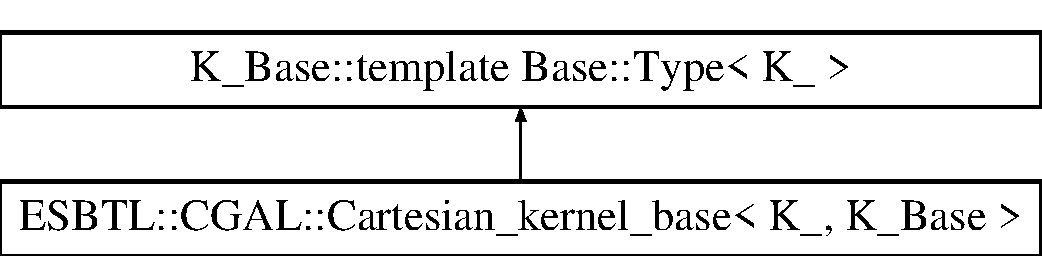
\includegraphics[height=2.000000cm]{classESBTL_1_1CGAL_1_1Cartesian__kernel__base}
\end{center}
\end{figure}
\subsection*{Classes}
\begin{DoxyCompactItemize}
\item 
struct \hyperlink{structESBTL_1_1CGAL_1_1Cartesian__kernel__base_1_1Base}{Base}
\end{DoxyCompactItemize}
\subsection*{Public Types}
\begin{DoxyCompactItemize}
\item 
typedef K\+\_\+ \hyperlink{classESBTL_1_1CGAL_1_1Cartesian__kernel__base_a281013f75db02ed3c77c1247776c4a00}{Kernel}
\item 
typedef \hyperlink{classESBTL_1_1Molecular__system}{Molecular\+\_\+system}$<$ \hyperlink{structESBTL_1_1Default__system__items}{Default\+\_\+system\+\_\+items}, typename K\+\_\+\+Base\+::\+Point\+\_\+3 $>$\+::Atom \hyperlink{classESBTL_1_1CGAL_1_1Cartesian__kernel__base_a9a2ac39990666886a8bc8254b608fdac}{Point\+\_\+3}
\end{DoxyCompactItemize}


\subsection{Member Typedef Documentation}
\mbox{\Hypertarget{classESBTL_1_1CGAL_1_1Cartesian__kernel__base_a281013f75db02ed3c77c1247776c4a00}\label{classESBTL_1_1CGAL_1_1Cartesian__kernel__base_a281013f75db02ed3c77c1247776c4a00}} 
\index{E\+S\+B\+T\+L\+::\+C\+G\+A\+L\+::\+Cartesian\+\_\+kernel\+\_\+base@{E\+S\+B\+T\+L\+::\+C\+G\+A\+L\+::\+Cartesian\+\_\+kernel\+\_\+base}!Kernel@{Kernel}}
\index{Kernel@{Kernel}!E\+S\+B\+T\+L\+::\+C\+G\+A\+L\+::\+Cartesian\+\_\+kernel\+\_\+base@{E\+S\+B\+T\+L\+::\+C\+G\+A\+L\+::\+Cartesian\+\_\+kernel\+\_\+base}}
\subsubsection{\texorpdfstring{Kernel}{Kernel}}
{\footnotesize\ttfamily template$<$typename K\+\_\+ , typename K\+\_\+\+Base $>$ \\
typedef K\+\_\+ \hyperlink{classESBTL_1_1CGAL_1_1Cartesian__kernel__base}{E\+S\+B\+T\+L\+::\+C\+G\+A\+L\+::\+Cartesian\+\_\+kernel\+\_\+base}$<$ K\+\_\+, K\+\_\+\+Base $>$\+::\hyperlink{classESBTL_1_1CGAL_1_1Cartesian__kernel__base_a281013f75db02ed3c77c1247776c4a00}{Kernel}}

\mbox{\Hypertarget{classESBTL_1_1CGAL_1_1Cartesian__kernel__base_a9a2ac39990666886a8bc8254b608fdac}\label{classESBTL_1_1CGAL_1_1Cartesian__kernel__base_a9a2ac39990666886a8bc8254b608fdac}} 
\index{E\+S\+B\+T\+L\+::\+C\+G\+A\+L\+::\+Cartesian\+\_\+kernel\+\_\+base@{E\+S\+B\+T\+L\+::\+C\+G\+A\+L\+::\+Cartesian\+\_\+kernel\+\_\+base}!Point\+\_\+3@{Point\+\_\+3}}
\index{Point\+\_\+3@{Point\+\_\+3}!E\+S\+B\+T\+L\+::\+C\+G\+A\+L\+::\+Cartesian\+\_\+kernel\+\_\+base@{E\+S\+B\+T\+L\+::\+C\+G\+A\+L\+::\+Cartesian\+\_\+kernel\+\_\+base}}
\subsubsection{\texorpdfstring{Point\+\_\+3}{Point\_3}}
{\footnotesize\ttfamily template$<$typename K\+\_\+ , typename K\+\_\+\+Base $>$ \\
typedef \hyperlink{classESBTL_1_1Molecular__system}{Molecular\+\_\+system}$<$\hyperlink{structESBTL_1_1Default__system__items}{Default\+\_\+system\+\_\+items},typename K\+\_\+\+Base\+::\+Point\+\_\+3 $>$\+::Atom \hyperlink{classESBTL_1_1CGAL_1_1Cartesian__kernel__base}{E\+S\+B\+T\+L\+::\+C\+G\+A\+L\+::\+Cartesian\+\_\+kernel\+\_\+base}$<$ K\+\_\+, K\+\_\+\+Base $>$\+::\hyperlink{classESBTL_1_1CGAL_1_1Cartesian__kernel__base_a9a2ac39990666886a8bc8254b608fdac}{Point\+\_\+3}}



The documentation for this class was generated from the following file\+:\begin{DoxyCompactItemize}
\item 
C\+G\+A\+L/\hyperlink{EPIC__kernel__with__atom_8h}{E\+P\+I\+C\+\_\+kernel\+\_\+with\+\_\+atom.\+h}\end{DoxyCompactItemize}

\hypertarget{classESBTL_1_1CGAL_1_1Cartesian__kernel__base__cg}{}\section{E\+S\+B\+TL\+:\+:C\+G\+AL\+:\+:Cartesian\+\_\+kernel\+\_\+base\+\_\+cg$<$ K\+\_\+, K\+\_\+\+Base $>$ Class Template Reference}
\label{classESBTL_1_1CGAL_1_1Cartesian__kernel__base__cg}\index{E\+S\+B\+T\+L\+::\+C\+G\+A\+L\+::\+Cartesian\+\_\+kernel\+\_\+base\+\_\+cg$<$ K\+\_\+, K\+\_\+\+Base $>$@{E\+S\+B\+T\+L\+::\+C\+G\+A\+L\+::\+Cartesian\+\_\+kernel\+\_\+base\+\_\+cg$<$ K\+\_\+, K\+\_\+\+Base $>$}}


{\ttfamily \#include $<$E\+P\+I\+C\+\_\+kernel\+\_\+with\+\_\+atom.\+h$>$}

Inheritance diagram for E\+S\+B\+TL\+:\+:C\+G\+AL\+:\+:Cartesian\+\_\+kernel\+\_\+base\+\_\+cg$<$ K\+\_\+, K\+\_\+\+Base $>$\+:\begin{figure}[H]
\begin{center}
\leavevmode
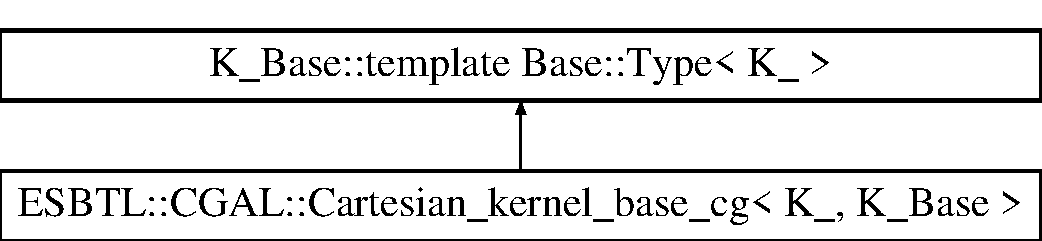
\includegraphics[height=2.000000cm]{classESBTL_1_1CGAL_1_1Cartesian__kernel__base__cg}
\end{center}
\end{figure}
\subsection*{Classes}
\begin{DoxyCompactItemize}
\item 
struct \hyperlink{structESBTL_1_1CGAL_1_1Cartesian__kernel__base__cg_1_1Base}{Base}
\end{DoxyCompactItemize}
\subsection*{Public Types}
\begin{DoxyCompactItemize}
\item 
typedef K\+\_\+ \hyperlink{classESBTL_1_1CGAL_1_1Cartesian__kernel__base__cg_a0e4e4792eb3643c5f639481e54d3da79}{Kernel}
\item 
typedef \hyperlink{classESBTL_1_1Coarse__atom}{Coarse\+\_\+atom}$<$ Atom, typename K\+\_\+\+Base\+::\+Point\+\_\+3 $>$ \hyperlink{classESBTL_1_1CGAL_1_1Cartesian__kernel__base__cg_a332637869c2baa408be0c6f537f7929d}{Point\+\_\+3}
\end{DoxyCompactItemize}


\subsection{Member Typedef Documentation}
\mbox{\Hypertarget{classESBTL_1_1CGAL_1_1Cartesian__kernel__base__cg_a0e4e4792eb3643c5f639481e54d3da79}\label{classESBTL_1_1CGAL_1_1Cartesian__kernel__base__cg_a0e4e4792eb3643c5f639481e54d3da79}} 
\index{E\+S\+B\+T\+L\+::\+C\+G\+A\+L\+::\+Cartesian\+\_\+kernel\+\_\+base\+\_\+cg@{E\+S\+B\+T\+L\+::\+C\+G\+A\+L\+::\+Cartesian\+\_\+kernel\+\_\+base\+\_\+cg}!Kernel@{Kernel}}
\index{Kernel@{Kernel}!E\+S\+B\+T\+L\+::\+C\+G\+A\+L\+::\+Cartesian\+\_\+kernel\+\_\+base\+\_\+cg@{E\+S\+B\+T\+L\+::\+C\+G\+A\+L\+::\+Cartesian\+\_\+kernel\+\_\+base\+\_\+cg}}
\subsubsection{\texorpdfstring{Kernel}{Kernel}}
{\footnotesize\ttfamily template$<$typename K\+\_\+ , typename K\+\_\+\+Base $>$ \\
typedef K\+\_\+ \hyperlink{classESBTL_1_1CGAL_1_1Cartesian__kernel__base__cg}{E\+S\+B\+T\+L\+::\+C\+G\+A\+L\+::\+Cartesian\+\_\+kernel\+\_\+base\+\_\+cg}$<$ K\+\_\+, K\+\_\+\+Base $>$\+::\hyperlink{classESBTL_1_1CGAL_1_1Cartesian__kernel__base__cg_a0e4e4792eb3643c5f639481e54d3da79}{Kernel}}

\mbox{\Hypertarget{classESBTL_1_1CGAL_1_1Cartesian__kernel__base__cg_a332637869c2baa408be0c6f537f7929d}\label{classESBTL_1_1CGAL_1_1Cartesian__kernel__base__cg_a332637869c2baa408be0c6f537f7929d}} 
\index{E\+S\+B\+T\+L\+::\+C\+G\+A\+L\+::\+Cartesian\+\_\+kernel\+\_\+base\+\_\+cg@{E\+S\+B\+T\+L\+::\+C\+G\+A\+L\+::\+Cartesian\+\_\+kernel\+\_\+base\+\_\+cg}!Point\+\_\+3@{Point\+\_\+3}}
\index{Point\+\_\+3@{Point\+\_\+3}!E\+S\+B\+T\+L\+::\+C\+G\+A\+L\+::\+Cartesian\+\_\+kernel\+\_\+base\+\_\+cg@{E\+S\+B\+T\+L\+::\+C\+G\+A\+L\+::\+Cartesian\+\_\+kernel\+\_\+base\+\_\+cg}}
\subsubsection{\texorpdfstring{Point\+\_\+3}{Point\_3}}
{\footnotesize\ttfamily template$<$typename K\+\_\+ , typename K\+\_\+\+Base $>$ \\
typedef \hyperlink{classESBTL_1_1Coarse__atom}{Coarse\+\_\+atom}$<$Atom,typename K\+\_\+\+Base\+::\+Point\+\_\+3$>$ \hyperlink{classESBTL_1_1CGAL_1_1Cartesian__kernel__base__cg}{E\+S\+B\+T\+L\+::\+C\+G\+A\+L\+::\+Cartesian\+\_\+kernel\+\_\+base\+\_\+cg}$<$ K\+\_\+, K\+\_\+\+Base $>$\+::\hyperlink{classESBTL_1_1CGAL_1_1Cartesian__kernel__base__cg_a332637869c2baa408be0c6f537f7929d}{Point\+\_\+3}}



The documentation for this class was generated from the following file\+:\begin{DoxyCompactItemize}
\item 
C\+G\+A\+L/\hyperlink{EPIC__kernel__with__atom_8h}{E\+P\+I\+C\+\_\+kernel\+\_\+with\+\_\+atom.\+h}\end{DoxyCompactItemize}

\hypertarget{structESBTL_1_1Default__system__items_1_1Chain__wrapper}{}\section{E\+S\+B\+TL\+:\+:Default\+\_\+system\+\_\+items\+:\+:Chain\+\_\+wrapper$<$ System, Point $>$ Struct Template Reference}
\label{structESBTL_1_1Default__system__items_1_1Chain__wrapper}\index{E\+S\+B\+T\+L\+::\+Default\+\_\+system\+\_\+items\+::\+Chain\+\_\+wrapper$<$ System, Point $>$@{E\+S\+B\+T\+L\+::\+Default\+\_\+system\+\_\+items\+::\+Chain\+\_\+wrapper$<$ System, Point $>$}}


{\ttfamily \#include $<$molecular\+\_\+system.\+h$>$}

\subsection*{Public Types}
\begin{DoxyCompactItemize}
\item 
typedef \hyperlink{classESBTL_1_1Molecular__chain}{Molecular\+\_\+chain}$<$ System $>$ \hyperlink{structESBTL_1_1Default__system__items_1_1Chain__wrapper_a4cb2f7c67fd8cdddefca890bbf5a49f2}{Type}
\end{DoxyCompactItemize}


\subsection{Member Typedef Documentation}
\mbox{\Hypertarget{structESBTL_1_1Default__system__items_1_1Chain__wrapper_a4cb2f7c67fd8cdddefca890bbf5a49f2}\label{structESBTL_1_1Default__system__items_1_1Chain__wrapper_a4cb2f7c67fd8cdddefca890bbf5a49f2}} 
\index{E\+S\+B\+T\+L\+::\+Default\+\_\+system\+\_\+items\+::\+Chain\+\_\+wrapper@{E\+S\+B\+T\+L\+::\+Default\+\_\+system\+\_\+items\+::\+Chain\+\_\+wrapper}!Type@{Type}}
\index{Type@{Type}!E\+S\+B\+T\+L\+::\+Default\+\_\+system\+\_\+items\+::\+Chain\+\_\+wrapper@{E\+S\+B\+T\+L\+::\+Default\+\_\+system\+\_\+items\+::\+Chain\+\_\+wrapper}}
\subsubsection{\texorpdfstring{Type}{Type}}
{\footnotesize\ttfamily template$<$class System , class Point $>$ \\
typedef \hyperlink{classESBTL_1_1Molecular__chain}{Molecular\+\_\+chain}$<$System$>$ \hyperlink{structESBTL_1_1Default__system__items_1_1Chain__wrapper}{E\+S\+B\+T\+L\+::\+Default\+\_\+system\+\_\+items\+::\+Chain\+\_\+wrapper}$<$ System, Point $>$\+::\hyperlink{structESBTL_1_1Default__system__items_1_1Chain__wrapper_a4cb2f7c67fd8cdddefca890bbf5a49f2}{Type}}



The documentation for this struct was generated from the following file\+:\begin{DoxyCompactItemize}
\item 
\hyperlink{molecular__system_8h}{molecular\+\_\+system.\+h}\end{DoxyCompactItemize}

\hypertarget{structESBTL_1_1System__items__with__coarse__grain_1_1Chain__wrapper}{}\section{E\+S\+B\+TL\+:\+:System\+\_\+items\+\_\+with\+\_\+coarse\+\_\+grain\+:\+:Chain\+\_\+wrapper$<$ System, Point\+\_\+3 $>$ Struct Template Reference}
\label{structESBTL_1_1System__items__with__coarse__grain_1_1Chain__wrapper}\index{E\+S\+B\+T\+L\+::\+System\+\_\+items\+\_\+with\+\_\+coarse\+\_\+grain\+::\+Chain\+\_\+wrapper$<$ System, Point\+\_\+3 $>$@{E\+S\+B\+T\+L\+::\+System\+\_\+items\+\_\+with\+\_\+coarse\+\_\+grain\+::\+Chain\+\_\+wrapper$<$ System, Point\+\_\+3 $>$}}


{\ttfamily \#include $<$coarse\+\_\+grain.\+h$>$}

\subsection*{Public Types}
\begin{DoxyCompactItemize}
\item 
typedef \hyperlink{classESBTL_1_1Molecular__chain}{Molecular\+\_\+chain}$<$ System $>$ \hyperlink{structESBTL_1_1System__items__with__coarse__grain_1_1Chain__wrapper_a5fbb0ec01f257013da71c37fb855da2d}{Type}
\end{DoxyCompactItemize}


\subsection{Member Typedef Documentation}
\mbox{\Hypertarget{structESBTL_1_1System__items__with__coarse__grain_1_1Chain__wrapper_a5fbb0ec01f257013da71c37fb855da2d}\label{structESBTL_1_1System__items__with__coarse__grain_1_1Chain__wrapper_a5fbb0ec01f257013da71c37fb855da2d}} 
\index{E\+S\+B\+T\+L\+::\+System\+\_\+items\+\_\+with\+\_\+coarse\+\_\+grain\+::\+Chain\+\_\+wrapper@{E\+S\+B\+T\+L\+::\+System\+\_\+items\+\_\+with\+\_\+coarse\+\_\+grain\+::\+Chain\+\_\+wrapper}!Type@{Type}}
\index{Type@{Type}!E\+S\+B\+T\+L\+::\+System\+\_\+items\+\_\+with\+\_\+coarse\+\_\+grain\+::\+Chain\+\_\+wrapper@{E\+S\+B\+T\+L\+::\+System\+\_\+items\+\_\+with\+\_\+coarse\+\_\+grain\+::\+Chain\+\_\+wrapper}}
\subsubsection{\texorpdfstring{Type}{Type}}
{\footnotesize\ttfamily template$<$class System , class Point\+\_\+3 $>$ \\
typedef \hyperlink{classESBTL_1_1Molecular__chain}{Molecular\+\_\+chain}$<$System$>$ \hyperlink{structESBTL_1_1System__items__with__coarse__grain_1_1Chain__wrapper}{E\+S\+B\+T\+L\+::\+System\+\_\+items\+\_\+with\+\_\+coarse\+\_\+grain\+::\+Chain\+\_\+wrapper}$<$ System, \hyperlink{classESBTL_1_1Point__3}{Point\+\_\+3} $>$\+::\hyperlink{structESBTL_1_1System__items__with__coarse__grain_1_1Chain__wrapper_a5fbb0ec01f257013da71c37fb855da2d}{Type}}



The documentation for this struct was generated from the following file\+:\begin{DoxyCompactItemize}
\item 
\hyperlink{coarse__grain_8h}{coarse\+\_\+grain.\+h}\end{DoxyCompactItemize}

\hypertarget{classESBTL_1_1Coarse__atom}{}\section{E\+S\+B\+TL\+:\+:Coarse\+\_\+atom$<$ Atom, Point $>$ Class Template Reference}
\label{classESBTL_1_1Coarse__atom}\index{E\+S\+B\+T\+L\+::\+Coarse\+\_\+atom$<$ Atom, Point $>$@{E\+S\+B\+T\+L\+::\+Coarse\+\_\+atom$<$ Atom, Point $>$}}


{\ttfamily \#include $<$coarse\+\_\+grain.\+h$>$}

Inheritance diagram for E\+S\+B\+TL\+:\+:Coarse\+\_\+atom$<$ Atom, Point $>$\+:\begin{figure}[H]
\begin{center}
\leavevmode
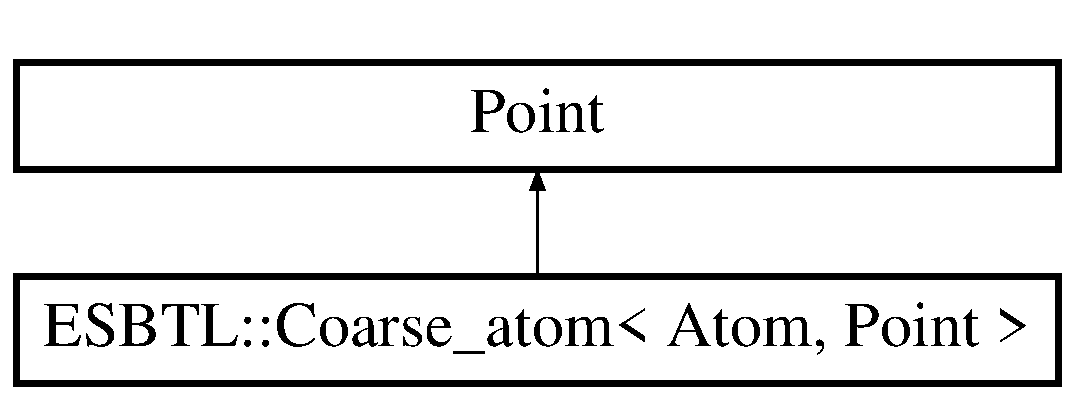
\includegraphics[height=2.000000cm]{classESBTL_1_1Coarse__atom}
\end{center}
\end{figure}
\subsection*{Public Types}
\begin{DoxyCompactItemize}
\item 
typedef Point \hyperlink{classESBTL_1_1Coarse__atom_acfe6c03e22cc26daef4776e7ca8a7db6}{Point\+\_\+3}
\end{DoxyCompactItemize}
\subsection*{Public Member Functions}
\begin{DoxyCompactItemize}
\item 
void \hyperlink{classESBTL_1_1Coarse__atom_a4cd2e08c968eac9e00493e4d43e24557}{add} (const Atom \&atom)
\item 
\hyperlink{classESBTL_1_1Coarse__atom_ae1eb9078c6062f775c1390272c6764a9}{Coarse\+\_\+atom} (const \hyperlink{classESBTL_1_1Coarse__atom_acfe6c03e22cc26daef4776e7ca8a7db6}{Point\+\_\+3} \&p, unsigned i, const Residue \&res)
\item 
\hyperlink{classESBTL_1_1Coarse__atom_a799d08aa0f138973750012a43f6428b9}{Coarse\+\_\+atom} (unsigned i, const Residue \&res)
\item 
\hyperlink{classESBTL_1_1Coarse__atom_a91362ec8871caea4dcc7b0822bd4be9c}{Coarse\+\_\+atom} ()
\item 
\hyperlink{classESBTL_1_1Coarse__atom_a127c90585bdd67131ff4159662bbd917}{Coarse\+\_\+atom} (float x, float y, float z)
\item 
const Residue \& \hyperlink{classESBTL_1_1Coarse__atom_ab07cf33f1040349d5af862f147dbc022}{residue} () const
\item 
unsigned \hyperlink{classESBTL_1_1Coarse__atom_adf0d8955c898d77d6040dec96be9fed1}{index} () const
\end{DoxyCompactItemize}


\subsection{Detailed Description}
\subsubsection*{template$<$class Atom, class Point$>$\newline
class E\+S\+B\+T\+L\+::\+Coarse\+\_\+atom$<$ Atom, Point $>$}

A coarse-\/grain atom type 
\begin{DoxyTemplParams}{Template Parameters}
{\em Atom} & is the base atom class that the coarse atom represent. \\
\hline
{\em Point} & is a point type with coordinates const access methods x(), y() and z(). \\
\hline
\end{DoxyTemplParams}


\subsection{Member Typedef Documentation}
\mbox{\Hypertarget{classESBTL_1_1Coarse__atom_acfe6c03e22cc26daef4776e7ca8a7db6}\label{classESBTL_1_1Coarse__atom_acfe6c03e22cc26daef4776e7ca8a7db6}} 
\index{E\+S\+B\+T\+L\+::\+Coarse\+\_\+atom@{E\+S\+B\+T\+L\+::\+Coarse\+\_\+atom}!Point\+\_\+3@{Point\+\_\+3}}
\index{Point\+\_\+3@{Point\+\_\+3}!E\+S\+B\+T\+L\+::\+Coarse\+\_\+atom@{E\+S\+B\+T\+L\+::\+Coarse\+\_\+atom}}
\subsubsection{\texorpdfstring{Point\+\_\+3}{Point\_3}}
{\footnotesize\ttfamily template$<$class Atom , class Point $>$ \\
typedef Point \hyperlink{classESBTL_1_1Coarse__atom}{E\+S\+B\+T\+L\+::\+Coarse\+\_\+atom}$<$ Atom, Point $>$\+::\hyperlink{classESBTL_1_1Coarse__atom_acfe6c03e22cc26daef4776e7ca8a7db6}{Point\+\_\+3}}



\subsection{Constructor \& Destructor Documentation}
\mbox{\Hypertarget{classESBTL_1_1Coarse__atom_ae1eb9078c6062f775c1390272c6764a9}\label{classESBTL_1_1Coarse__atom_ae1eb9078c6062f775c1390272c6764a9}} 
\index{E\+S\+B\+T\+L\+::\+Coarse\+\_\+atom@{E\+S\+B\+T\+L\+::\+Coarse\+\_\+atom}!Coarse\+\_\+atom@{Coarse\+\_\+atom}}
\index{Coarse\+\_\+atom@{Coarse\+\_\+atom}!E\+S\+B\+T\+L\+::\+Coarse\+\_\+atom@{E\+S\+B\+T\+L\+::\+Coarse\+\_\+atom}}
\subsubsection{\texorpdfstring{Coarse\+\_\+atom()}{Coarse\_atom()}\hspace{0.1cm}{\footnotesize\ttfamily [1/4]}}
{\footnotesize\ttfamily template$<$class Atom , class Point $>$ \\
\hyperlink{classESBTL_1_1Coarse__atom}{E\+S\+B\+T\+L\+::\+Coarse\+\_\+atom}$<$ Atom, Point $>$\+::\hyperlink{classESBTL_1_1Coarse__atom}{Coarse\+\_\+atom} (\begin{DoxyParamCaption}\item[{const \hyperlink{classESBTL_1_1Coarse__atom_acfe6c03e22cc26daef4776e7ca8a7db6}{Point\+\_\+3} \&}]{p,  }\item[{unsigned}]{i,  }\item[{const Residue \&}]{res }\end{DoxyParamCaption})\hspace{0.3cm}{\ttfamily [inline]}}

\mbox{\Hypertarget{classESBTL_1_1Coarse__atom_a799d08aa0f138973750012a43f6428b9}\label{classESBTL_1_1Coarse__atom_a799d08aa0f138973750012a43f6428b9}} 
\index{E\+S\+B\+T\+L\+::\+Coarse\+\_\+atom@{E\+S\+B\+T\+L\+::\+Coarse\+\_\+atom}!Coarse\+\_\+atom@{Coarse\+\_\+atom}}
\index{Coarse\+\_\+atom@{Coarse\+\_\+atom}!E\+S\+B\+T\+L\+::\+Coarse\+\_\+atom@{E\+S\+B\+T\+L\+::\+Coarse\+\_\+atom}}
\subsubsection{\texorpdfstring{Coarse\+\_\+atom()}{Coarse\_atom()}\hspace{0.1cm}{\footnotesize\ttfamily [2/4]}}
{\footnotesize\ttfamily template$<$class Atom , class Point $>$ \\
\hyperlink{classESBTL_1_1Coarse__atom}{E\+S\+B\+T\+L\+::\+Coarse\+\_\+atom}$<$ Atom, Point $>$\+::\hyperlink{classESBTL_1_1Coarse__atom}{Coarse\+\_\+atom} (\begin{DoxyParamCaption}\item[{unsigned}]{i,  }\item[{const Residue \&}]{res }\end{DoxyParamCaption})\hspace{0.3cm}{\ttfamily [inline]}}

\mbox{\Hypertarget{classESBTL_1_1Coarse__atom_a91362ec8871caea4dcc7b0822bd4be9c}\label{classESBTL_1_1Coarse__atom_a91362ec8871caea4dcc7b0822bd4be9c}} 
\index{E\+S\+B\+T\+L\+::\+Coarse\+\_\+atom@{E\+S\+B\+T\+L\+::\+Coarse\+\_\+atom}!Coarse\+\_\+atom@{Coarse\+\_\+atom}}
\index{Coarse\+\_\+atom@{Coarse\+\_\+atom}!E\+S\+B\+T\+L\+::\+Coarse\+\_\+atom@{E\+S\+B\+T\+L\+::\+Coarse\+\_\+atom}}
\subsubsection{\texorpdfstring{Coarse\+\_\+atom()}{Coarse\_atom()}\hspace{0.1cm}{\footnotesize\ttfamily [3/4]}}
{\footnotesize\ttfamily template$<$class Atom , class Point $>$ \\
\hyperlink{classESBTL_1_1Coarse__atom}{E\+S\+B\+T\+L\+::\+Coarse\+\_\+atom}$<$ Atom, Point $>$\+::\hyperlink{classESBTL_1_1Coarse__atom}{Coarse\+\_\+atom} (\begin{DoxyParamCaption}{ }\end{DoxyParamCaption})\hspace{0.3cm}{\ttfamily [inline]}}

\mbox{\Hypertarget{classESBTL_1_1Coarse__atom_a127c90585bdd67131ff4159662bbd917}\label{classESBTL_1_1Coarse__atom_a127c90585bdd67131ff4159662bbd917}} 
\index{E\+S\+B\+T\+L\+::\+Coarse\+\_\+atom@{E\+S\+B\+T\+L\+::\+Coarse\+\_\+atom}!Coarse\+\_\+atom@{Coarse\+\_\+atom}}
\index{Coarse\+\_\+atom@{Coarse\+\_\+atom}!E\+S\+B\+T\+L\+::\+Coarse\+\_\+atom@{E\+S\+B\+T\+L\+::\+Coarse\+\_\+atom}}
\subsubsection{\texorpdfstring{Coarse\+\_\+atom()}{Coarse\_atom()}\hspace{0.1cm}{\footnotesize\ttfamily [4/4]}}
{\footnotesize\ttfamily template$<$class Atom , class Point $>$ \\
\hyperlink{classESBTL_1_1Coarse__atom}{E\+S\+B\+T\+L\+::\+Coarse\+\_\+atom}$<$ Atom, Point $>$\+::\hyperlink{classESBTL_1_1Coarse__atom}{Coarse\+\_\+atom} (\begin{DoxyParamCaption}\item[{float}]{x,  }\item[{float}]{y,  }\item[{float}]{z }\end{DoxyParamCaption})\hspace{0.3cm}{\ttfamily [inline]}}



\subsection{Member Function Documentation}
\mbox{\Hypertarget{classESBTL_1_1Coarse__atom_a4cd2e08c968eac9e00493e4d43e24557}\label{classESBTL_1_1Coarse__atom_a4cd2e08c968eac9e00493e4d43e24557}} 
\index{E\+S\+B\+T\+L\+::\+Coarse\+\_\+atom@{E\+S\+B\+T\+L\+::\+Coarse\+\_\+atom}!add@{add}}
\index{add@{add}!E\+S\+B\+T\+L\+::\+Coarse\+\_\+atom@{E\+S\+B\+T\+L\+::\+Coarse\+\_\+atom}}
\subsubsection{\texorpdfstring{add()}{add()}}
{\footnotesize\ttfamily template$<$class Atom , class Point $>$ \\
void \hyperlink{classESBTL_1_1Coarse__atom}{E\+S\+B\+T\+L\+::\+Coarse\+\_\+atom}$<$ Atom, Point $>$\+::add (\begin{DoxyParamCaption}\item[{const Atom \&}]{atom }\end{DoxyParamCaption})\hspace{0.3cm}{\ttfamily [inline]}}

Add atom to the set of atom represented. \mbox{\Hypertarget{classESBTL_1_1Coarse__atom_adf0d8955c898d77d6040dec96be9fed1}\label{classESBTL_1_1Coarse__atom_adf0d8955c898d77d6040dec96be9fed1}} 
\index{E\+S\+B\+T\+L\+::\+Coarse\+\_\+atom@{E\+S\+B\+T\+L\+::\+Coarse\+\_\+atom}!index@{index}}
\index{index@{index}!E\+S\+B\+T\+L\+::\+Coarse\+\_\+atom@{E\+S\+B\+T\+L\+::\+Coarse\+\_\+atom}}
\subsubsection{\texorpdfstring{index()}{index()}}
{\footnotesize\ttfamily template$<$class Atom , class Point $>$ \\
unsigned \hyperlink{classESBTL_1_1Coarse__atom}{E\+S\+B\+T\+L\+::\+Coarse\+\_\+atom}$<$ Atom, Point $>$\+::index (\begin{DoxyParamCaption}{ }\end{DoxyParamCaption}) const\hspace{0.3cm}{\ttfamily [inline]}}

\mbox{\Hypertarget{classESBTL_1_1Coarse__atom_ab07cf33f1040349d5af862f147dbc022}\label{classESBTL_1_1Coarse__atom_ab07cf33f1040349d5af862f147dbc022}} 
\index{E\+S\+B\+T\+L\+::\+Coarse\+\_\+atom@{E\+S\+B\+T\+L\+::\+Coarse\+\_\+atom}!residue@{residue}}
\index{residue@{residue}!E\+S\+B\+T\+L\+::\+Coarse\+\_\+atom@{E\+S\+B\+T\+L\+::\+Coarse\+\_\+atom}}
\subsubsection{\texorpdfstring{residue()}{residue()}}
{\footnotesize\ttfamily template$<$class Atom , class Point $>$ \\
const Residue\& \hyperlink{classESBTL_1_1Coarse__atom}{E\+S\+B\+T\+L\+::\+Coarse\+\_\+atom}$<$ Atom, Point $>$\+::residue (\begin{DoxyParamCaption}{ }\end{DoxyParamCaption}) const\hspace{0.3cm}{\ttfamily [inline]}}



The documentation for this class was generated from the following file\+:\begin{DoxyCompactItemize}
\item 
\hyperlink{coarse__grain_8h}{coarse\+\_\+grain.\+h}\end{DoxyCompactItemize}

\hypertarget{structESBTL_1_1Coarse__atoms__iterators}{}\section{E\+S\+B\+TL\+:\+:Coarse\+\_\+atoms\+\_\+iterators$<$ Model $>$ Struct Template Reference}
\label{structESBTL_1_1Coarse__atoms__iterators}\index{E\+S\+B\+T\+L\+::\+Coarse\+\_\+atoms\+\_\+iterators$<$ Model $>$@{E\+S\+B\+T\+L\+::\+Coarse\+\_\+atoms\+\_\+iterators$<$ Model $>$}}


{\ttfamily \#include $<$coarse\+\_\+grain.\+h$>$}

\subsection*{Public Types}
\begin{DoxyCompactItemize}
\item 
typedef internal\+::\+Coarse\+\_\+atom\+\_\+from\+\_\+model$<$ Model, true $>$ \hyperlink{structESBTL_1_1Coarse__atoms__iterators_acff1d0d843ccc6f72f18fa24b1b016db}{const\+\_\+iterator}
\item 
typedef internal\+::\+Coarse\+\_\+atom\+\_\+from\+\_\+model$<$ Model, false $>$ \hyperlink{structESBTL_1_1Coarse__atoms__iterators_adfb6d7bbe918849df2d701becde2c8d5}{iterator}
\end{DoxyCompactItemize}


\subsection{Detailed Description}
\subsubsection*{template$<$class Model$>$\newline
struct E\+S\+B\+T\+L\+::\+Coarse\+\_\+atoms\+\_\+iterators$<$ Model $>$}

Object defining iterator types over coarse grain residue of a model 
\begin{DoxyTemplParams}{Template Parameters}
{\em Model} & is the type of the model coarse grain atoms are read. \\
\hline
\end{DoxyTemplParams}


\subsection{Member Typedef Documentation}
\mbox{\Hypertarget{structESBTL_1_1Coarse__atoms__iterators_acff1d0d843ccc6f72f18fa24b1b016db}\label{structESBTL_1_1Coarse__atoms__iterators_acff1d0d843ccc6f72f18fa24b1b016db}} 
\index{E\+S\+B\+T\+L\+::\+Coarse\+\_\+atoms\+\_\+iterators@{E\+S\+B\+T\+L\+::\+Coarse\+\_\+atoms\+\_\+iterators}!const\+\_\+iterator@{const\+\_\+iterator}}
\index{const\+\_\+iterator@{const\+\_\+iterator}!E\+S\+B\+T\+L\+::\+Coarse\+\_\+atoms\+\_\+iterators@{E\+S\+B\+T\+L\+::\+Coarse\+\_\+atoms\+\_\+iterators}}
\subsubsection{\texorpdfstring{const\+\_\+iterator}{const\_iterator}}
{\footnotesize\ttfamily template$<$class Model$>$ \\
typedef internal\+::\+Coarse\+\_\+atom\+\_\+from\+\_\+model$<$Model,true$>$ \hyperlink{structESBTL_1_1Coarse__atoms__iterators}{E\+S\+B\+T\+L\+::\+Coarse\+\_\+atoms\+\_\+iterators}$<$ Model $>$\+::\hyperlink{structESBTL_1_1Coarse__atoms__iterators_acff1d0d843ccc6f72f18fa24b1b016db}{const\+\_\+iterator}}

\mbox{\Hypertarget{structESBTL_1_1Coarse__atoms__iterators_adfb6d7bbe918849df2d701becde2c8d5}\label{structESBTL_1_1Coarse__atoms__iterators_adfb6d7bbe918849df2d701becde2c8d5}} 
\index{E\+S\+B\+T\+L\+::\+Coarse\+\_\+atoms\+\_\+iterators@{E\+S\+B\+T\+L\+::\+Coarse\+\_\+atoms\+\_\+iterators}!iterator@{iterator}}
\index{iterator@{iterator}!E\+S\+B\+T\+L\+::\+Coarse\+\_\+atoms\+\_\+iterators@{E\+S\+B\+T\+L\+::\+Coarse\+\_\+atoms\+\_\+iterators}}
\subsubsection{\texorpdfstring{iterator}{iterator}}
{\footnotesize\ttfamily template$<$class Model$>$ \\
typedef internal\+::\+Coarse\+\_\+atom\+\_\+from\+\_\+model$<$Model,false$>$ \hyperlink{structESBTL_1_1Coarse__atoms__iterators}{E\+S\+B\+T\+L\+::\+Coarse\+\_\+atoms\+\_\+iterators}$<$ Model $>$\+::\hyperlink{structESBTL_1_1Coarse__atoms__iterators_adfb6d7bbe918849df2d701becde2c8d5}{iterator}}



The documentation for this struct was generated from the following file\+:\begin{DoxyCompactItemize}
\item 
\hyperlink{coarse__grain_8h}{coarse\+\_\+grain.\+h}\end{DoxyCompactItemize}

\hypertarget{classESBTL_1_1Coarse__creator__closest__to__barycenter}{}\section{E\+S\+B\+TL\+:\+:Coarse\+\_\+creator\+\_\+closest\+\_\+to\+\_\+barycenter$<$ Residue, F\+T\+\_\+ $>$ Class Template Reference}
\label{classESBTL_1_1Coarse__creator__closest__to__barycenter}\index{E\+S\+B\+T\+L\+::\+Coarse\+\_\+creator\+\_\+closest\+\_\+to\+\_\+barycenter$<$ Residue, F\+T\+\_\+ $>$@{E\+S\+B\+T\+L\+::\+Coarse\+\_\+creator\+\_\+closest\+\_\+to\+\_\+barycenter$<$ Residue, F\+T\+\_\+ $>$}}


{\ttfamily \#include $<$coarse\+\_\+creators.\+h$>$}

\subsection*{Public Member Functions}
\begin{DoxyCompactItemize}
\item 
{\footnotesize template$<$class Output\+\_\+iterator $>$ }\\int \hyperlink{classESBTL_1_1Coarse__creator__closest__to__barycenter_aa6921d3c94810e7564188b837cf40191}{operator()} (const Residue \&res, Output\+\_\+iterator out) const
\end{DoxyCompactItemize}
\subsection*{Static Public Member Functions}
\begin{DoxyCompactItemize}
\item 
static const std\+::string \hyperlink{classESBTL_1_1Coarse__creator__closest__to__barycenter_a22f90422bb755d78f11b3f34094de0b2}{info} ()
\end{DoxyCompactItemize}


\subsection{Detailed Description}
\subsubsection*{template$<$class Residue, class F\+T\+\_\+$>$\newline
class E\+S\+B\+T\+L\+::\+Coarse\+\_\+creator\+\_\+closest\+\_\+to\+\_\+barycenter$<$ Residue, F\+T\+\_\+ $>$}

Creator of a coarse grain model using one pseudo-\/atom centered at the atom closest to the barycenter of the side-\/chain and the C-\/alpha of a residue. These atoms are identified using the global function \hyperlink{namespaceESBTL_a117981ffccc18137b919af5c47a51b0d}{E\+S\+B\+T\+L\+::is\+\_\+side\+\_\+chain\+\_\+or\+\_\+\+CA}.


\begin{DoxyTemplParams}{Template Parameters}
{\em Residue} & is the coarse grain residue type used. \\
\hline
{\em F\+T\+\_\+} & is the number type of the coordinates. \\
\hline
\end{DoxyTemplParams}


\subsection{Member Function Documentation}
\mbox{\Hypertarget{classESBTL_1_1Coarse__creator__closest__to__barycenter_a22f90422bb755d78f11b3f34094de0b2}\label{classESBTL_1_1Coarse__creator__closest__to__barycenter_a22f90422bb755d78f11b3f34094de0b2}} 
\index{E\+S\+B\+T\+L\+::\+Coarse\+\_\+creator\+\_\+closest\+\_\+to\+\_\+barycenter@{E\+S\+B\+T\+L\+::\+Coarse\+\_\+creator\+\_\+closest\+\_\+to\+\_\+barycenter}!info@{info}}
\index{info@{info}!E\+S\+B\+T\+L\+::\+Coarse\+\_\+creator\+\_\+closest\+\_\+to\+\_\+barycenter@{E\+S\+B\+T\+L\+::\+Coarse\+\_\+creator\+\_\+closest\+\_\+to\+\_\+barycenter}}
\subsubsection{\texorpdfstring{info()}{info()}}
{\footnotesize\ttfamily template$<$class Residue , class F\+T\+\_\+ $>$ \\
static const std\+::string \hyperlink{classESBTL_1_1Coarse__creator__closest__to__barycenter}{E\+S\+B\+T\+L\+::\+Coarse\+\_\+creator\+\_\+closest\+\_\+to\+\_\+barycenter}$<$ Residue, F\+T\+\_\+ $>$\+::info (\begin{DoxyParamCaption}{ }\end{DoxyParamCaption})\hspace{0.3cm}{\ttfamily [inline]}, {\ttfamily [static]}}

\mbox{\Hypertarget{classESBTL_1_1Coarse__creator__closest__to__barycenter_aa6921d3c94810e7564188b837cf40191}\label{classESBTL_1_1Coarse__creator__closest__to__barycenter_aa6921d3c94810e7564188b837cf40191}} 
\index{E\+S\+B\+T\+L\+::\+Coarse\+\_\+creator\+\_\+closest\+\_\+to\+\_\+barycenter@{E\+S\+B\+T\+L\+::\+Coarse\+\_\+creator\+\_\+closest\+\_\+to\+\_\+barycenter}!operator()@{operator()}}
\index{operator()@{operator()}!E\+S\+B\+T\+L\+::\+Coarse\+\_\+creator\+\_\+closest\+\_\+to\+\_\+barycenter@{E\+S\+B\+T\+L\+::\+Coarse\+\_\+creator\+\_\+closest\+\_\+to\+\_\+barycenter}}
\subsubsection{\texorpdfstring{operator()()}{operator()()}}
{\footnotesize\ttfamily template$<$class Residue , class F\+T\+\_\+ $>$ \\
template$<$class Output\+\_\+iterator $>$ \\
int \hyperlink{classESBTL_1_1Coarse__creator__closest__to__barycenter}{E\+S\+B\+T\+L\+::\+Coarse\+\_\+creator\+\_\+closest\+\_\+to\+\_\+barycenter}$<$ Residue, F\+T\+\_\+ $>$\+::operator() (\begin{DoxyParamCaption}\item[{const Residue \&}]{res,  }\item[{Output\+\_\+iterator}]{out }\end{DoxyParamCaption}) const\hspace{0.3cm}{\ttfamily [inline]}}



The documentation for this class was generated from the following file\+:\begin{DoxyCompactItemize}
\item 
\hyperlink{coarse__creators_8h}{coarse\+\_\+creators.\+h}\end{DoxyCompactItemize}

\hypertarget{classESBTL_1_1Coarse__creator__two__barycenters}{}\section{E\+S\+B\+TL\+:\+:Coarse\+\_\+creator\+\_\+two\+\_\+barycenters$<$ Residue $>$ Class Template Reference}
\label{classESBTL_1_1Coarse__creator__two__barycenters}\index{E\+S\+B\+T\+L\+::\+Coarse\+\_\+creator\+\_\+two\+\_\+barycenters$<$ Residue $>$@{E\+S\+B\+T\+L\+::\+Coarse\+\_\+creator\+\_\+two\+\_\+barycenters$<$ Residue $>$}}


{\ttfamily \#include $<$coarse\+\_\+creators.\+h$>$}

\subsection*{Public Member Functions}
\begin{DoxyCompactItemize}
\item 
{\footnotesize template$<$class Output\+\_\+iterator $>$ }\\int \hyperlink{classESBTL_1_1Coarse__creator__two__barycenters_a1de8d90f25b81d0634625a221609a7f7}{operator()} (const Residue \&res, Output\+\_\+iterator out) const
\end{DoxyCompactItemize}
\subsection*{Static Public Member Functions}
\begin{DoxyCompactItemize}
\item 
static const std\+::string \hyperlink{classESBTL_1_1Coarse__creator__two__barycenters_a341b961a5e6a8a14b78c84ea9688a1d5}{info} ()
\end{DoxyCompactItemize}


\subsection{Detailed Description}
\subsubsection*{template$<$class Residue$>$\newline
class E\+S\+B\+T\+L\+::\+Coarse\+\_\+creator\+\_\+two\+\_\+barycenters$<$ Residue $>$}

Creator of a coarse grain model creating up to two pseudo-\/atoms\+: one as the barycenter of backbone atoms (if relevant) and one as the barycenter of non-\/barycenter atoms. Backbone atoms are identified using the global function \hyperlink{namespaceESBTL_a4848989585f87e3953075f09a1089dec}{E\+S\+B\+T\+L\+::is\+\_\+backbone}.


\begin{DoxyTemplParams}{Template Parameters}
{\em Residue} & is the coarse grain residue type used. \\
\hline
\end{DoxyTemplParams}


\subsection{Member Function Documentation}
\mbox{\Hypertarget{classESBTL_1_1Coarse__creator__two__barycenters_a341b961a5e6a8a14b78c84ea9688a1d5}\label{classESBTL_1_1Coarse__creator__two__barycenters_a341b961a5e6a8a14b78c84ea9688a1d5}} 
\index{E\+S\+B\+T\+L\+::\+Coarse\+\_\+creator\+\_\+two\+\_\+barycenters@{E\+S\+B\+T\+L\+::\+Coarse\+\_\+creator\+\_\+two\+\_\+barycenters}!info@{info}}
\index{info@{info}!E\+S\+B\+T\+L\+::\+Coarse\+\_\+creator\+\_\+two\+\_\+barycenters@{E\+S\+B\+T\+L\+::\+Coarse\+\_\+creator\+\_\+two\+\_\+barycenters}}
\subsubsection{\texorpdfstring{info()}{info()}}
{\footnotesize\ttfamily template$<$class Residue $>$ \\
static const std\+::string \hyperlink{classESBTL_1_1Coarse__creator__two__barycenters}{E\+S\+B\+T\+L\+::\+Coarse\+\_\+creator\+\_\+two\+\_\+barycenters}$<$ Residue $>$\+::info (\begin{DoxyParamCaption}{ }\end{DoxyParamCaption})\hspace{0.3cm}{\ttfamily [inline]}, {\ttfamily [static]}}

\mbox{\Hypertarget{classESBTL_1_1Coarse__creator__two__barycenters_a1de8d90f25b81d0634625a221609a7f7}\label{classESBTL_1_1Coarse__creator__two__barycenters_a1de8d90f25b81d0634625a221609a7f7}} 
\index{E\+S\+B\+T\+L\+::\+Coarse\+\_\+creator\+\_\+two\+\_\+barycenters@{E\+S\+B\+T\+L\+::\+Coarse\+\_\+creator\+\_\+two\+\_\+barycenters}!operator()@{operator()}}
\index{operator()@{operator()}!E\+S\+B\+T\+L\+::\+Coarse\+\_\+creator\+\_\+two\+\_\+barycenters@{E\+S\+B\+T\+L\+::\+Coarse\+\_\+creator\+\_\+two\+\_\+barycenters}}
\subsubsection{\texorpdfstring{operator()()}{operator()()}}
{\footnotesize\ttfamily template$<$class Residue $>$ \\
template$<$class Output\+\_\+iterator $>$ \\
int \hyperlink{classESBTL_1_1Coarse__creator__two__barycenters}{E\+S\+B\+T\+L\+::\+Coarse\+\_\+creator\+\_\+two\+\_\+barycenters}$<$ Residue $>$\+::operator() (\begin{DoxyParamCaption}\item[{const Residue \&}]{res,  }\item[{Output\+\_\+iterator}]{out }\end{DoxyParamCaption}) const\hspace{0.3cm}{\ttfamily [inline]}}



The documentation for this class was generated from the following file\+:\begin{DoxyCompactItemize}
\item 
\hyperlink{coarse__creators_8h}{coarse\+\_\+creators.\+h}\end{DoxyCompactItemize}

\hypertarget{classESBTL_1_1Coarse__residue}{}\section{E\+S\+B\+TL\+:\+:Coarse\+\_\+residue$<$ Residue, Chain, Coarse\+\_\+atom\+\_\+ $>$ Class Template Reference}
\label{classESBTL_1_1Coarse__residue}\index{E\+S\+B\+T\+L\+::\+Coarse\+\_\+residue$<$ Residue, Chain, Coarse\+\_\+atom\+\_\+ $>$@{E\+S\+B\+T\+L\+::\+Coarse\+\_\+residue$<$ Residue, Chain, Coarse\+\_\+atom\+\_\+ $>$}}


{\ttfamily \#include $<$coarse\+\_\+grain.\+h$>$}

Inheritance diagram for E\+S\+B\+TL\+:\+:Coarse\+\_\+residue$<$ Residue, Chain, Coarse\+\_\+atom\+\_\+ $>$\+:\begin{figure}[H]
\begin{center}
\leavevmode
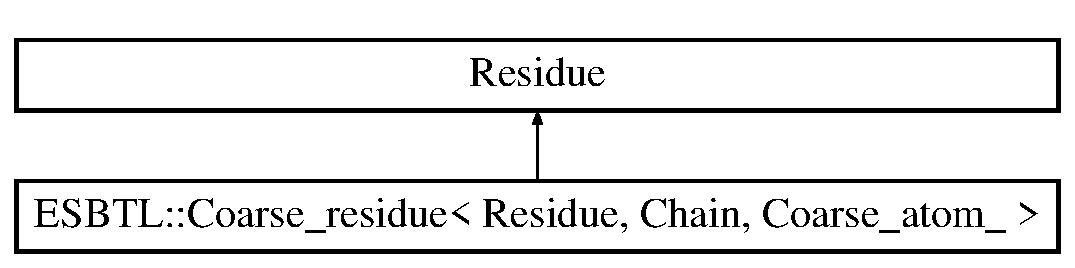
\includegraphics[height=2.000000cm]{classESBTL_1_1Coarse__residue}
\end{center}
\end{figure}
\subsection*{Public Types}
\begin{DoxyCompactItemize}
\item 
typedef std\+::vector$<$ Coarse\+\_\+atom\+\_\+ $>$ \hyperlink{classESBTL_1_1Coarse__residue_ac1fa9270ab6914abefb8e63ceeb5ba1f}{Coarse\+\_\+atom\+\_\+container}
\item 
typedef Coarse\+\_\+atom\+\_\+ \hyperlink{classESBTL_1_1Coarse__residue_a4e83dc008345f6b828bcd3a67045a051}{Coarse\+\_\+atom}
\item 
typedef Residue\+::\+Atom \hyperlink{classESBTL_1_1Coarse__residue_a3b6c0c25f9f2e005ef2d5888073214f0}{Atom}
\item 
typedef internal\+::\+Atoms\+\_\+iterator\+\_\+from\+\_\+residue$<$ \hyperlink{classESBTL_1_1Coarse__residue}{Self}, true $>$ \hyperlink{group__grp__iters_gabb95e73700fd84dbde6e089927e03a6d}{Atoms\+\_\+const\+\_\+iterator}
\item 
typedef internal\+::\+Atoms\+\_\+iterator\+\_\+from\+\_\+residue$<$ \hyperlink{classESBTL_1_1Coarse__residue}{Self}, false $>$ \hyperlink{group__grp__iters_ga8081408a6d91ed2a777111e2b2651ad4}{Atoms\+\_\+iterator}
\item 
typedef std\+::vector$<$ Coarse\+\_\+atom\+\_\+ $>$\+::const\+\_\+iterator \hyperlink{group__grp__iters_ga5a4a865846cdde342538df7fc03c80ce}{Coarse\+\_\+atom\+\_\+const\+\_\+iterator}
\item 
typedef std\+::vector$<$ Coarse\+\_\+atom\+\_\+ $>$\+::iterator \hyperlink{group__grp__iters_ga09a38741d50d3b7296dae83eb0911e49}{Coarse\+\_\+atom\+\_\+iterator}
\end{DoxyCompactItemize}
\subsection*{Public Member Functions}
\begin{DoxyCompactItemize}
\item 
{\footnotesize template$<$class Line\+\_\+format $>$ }\\\hyperlink{classESBTL_1_1Coarse__residue_aebedf19bfbb8c04f7413b1618bc5dd32}{Coarse\+\_\+residue} (const Line\+\_\+format \&line\+\_\+format, const std\+::string \&line, const Chain \&ch)
\item 
\hyperlink{classESBTL_1_1Coarse__residue_abde8049914cf69701dbe59f860887bab}{Coarse\+\_\+residue} (const std\+::string \&resname, int index, char insc, const Chain \&ch)
\item 
{\footnotesize template$<$class Coarse\+\_\+creator $>$ }\\int \hyperlink{classESBTL_1_1Coarse__residue_a4a514a6142ad550ade5df531f08d9cdd}{create\+\_\+coarse\+\_\+atoms} (const Coarse\+\_\+creator \&creator)
\item 
void \hyperlink{classESBTL_1_1Coarse__residue_ac261019b3966c7fd3c921217e335c11e}{add\+\_\+coarse\+\_\+atom} (const typename Residue\+::\+Atom\+::\+Point\+\_\+3 \&pt, unsigned i=0)
\item 
const \hyperlink{classESBTL_1_1Coarse__residue_a4e83dc008345f6b828bcd3a67045a051}{Coarse\+\_\+atom} \hyperlink{classESBTL_1_1Coarse__residue_a2dd7b7ebb517675fdb74b006f36d61fc}{get\+\_\+coarse\+\_\+atom} (unsigned i) const
\item 
\hyperlink{group__grp__iters_ga8081408a6d91ed2a777111e2b2651ad4}{Atoms\+\_\+iterator} \hyperlink{group__grp__iters_ga35aadf6bfc69effe4dd4a55b09e8a1ca}{atoms\+\_\+begin} ()
\item 
\hyperlink{group__grp__iters_ga8081408a6d91ed2a777111e2b2651ad4}{Atoms\+\_\+iterator} \hyperlink{group__grp__iters_ga71c3a50b585303176a530b52265b1b9c}{atoms\+\_\+end} ()
\item 
\hyperlink{group__grp__iters_gabb95e73700fd84dbde6e089927e03a6d}{Atoms\+\_\+const\+\_\+iterator} \hyperlink{group__grp__iters_ga9f73288663701102c207280c7af5a523}{atoms\+\_\+begin} () const
\item 
\hyperlink{group__grp__iters_gabb95e73700fd84dbde6e089927e03a6d}{Atoms\+\_\+const\+\_\+iterator} \hyperlink{group__grp__iters_gafa5493ec6a094421db2bfbaf17af3a90}{atoms\+\_\+end} () const
\item 
\hyperlink{group__grp__iters_ga5a4a865846cdde342538df7fc03c80ce}{Coarse\+\_\+atom\+\_\+const\+\_\+iterator} \hyperlink{group__grp__iters_gac0e520e0a924be52cfdfae8921a21d21}{coarse\+\_\+atoms\+\_\+begin} () const
\item 
\hyperlink{group__grp__iters_ga5a4a865846cdde342538df7fc03c80ce}{Coarse\+\_\+atom\+\_\+const\+\_\+iterator} \hyperlink{group__grp__iters_ga50026c05f269eddb69d9d775df51e442}{coarse\+\_\+atoms\+\_\+end} () const
\item 
\hyperlink{group__grp__iters_ga09a38741d50d3b7296dae83eb0911e49}{Coarse\+\_\+atom\+\_\+iterator} \hyperlink{group__grp__iters_gab001b6ad15d74ee2879ccc4669e52962}{coarse\+\_\+atoms\+\_\+begin} ()
\item 
\hyperlink{group__grp__iters_ga09a38741d50d3b7296dae83eb0911e49}{Coarse\+\_\+atom\+\_\+iterator} \hyperlink{group__grp__iters_ga2594d683372e0e198f725d8bd1577adf}{coarse\+\_\+atoms\+\_\+end} ()
\end{DoxyCompactItemize}
\subsection*{Static Public Member Functions}
\begin{DoxyCompactItemize}
\item 
static const \hyperlink{classESBTL_1_1Coarse__residue_a4e83dc008345f6b828bcd3a67045a051}{Coarse\+\_\+atom} \& \hyperlink{classESBTL_1_1Coarse__residue_a85c3825ca10ace200a4f2d4d626a81b0}{dereference} (\hyperlink{group__grp__iters_ga5a4a865846cdde342538df7fc03c80ce}{Coarse\+\_\+atom\+\_\+const\+\_\+iterator} it)
\item 
static \hyperlink{classESBTL_1_1Coarse__residue_a4e83dc008345f6b828bcd3a67045a051}{Coarse\+\_\+atom} \& \hyperlink{classESBTL_1_1Coarse__residue_aa3fa145ffbe14ab960c2baa41b6a0761}{dereference} (\hyperlink{group__grp__iters_ga09a38741d50d3b7296dae83eb0911e49}{Coarse\+\_\+atom\+\_\+iterator} it)
\end{DoxyCompactItemize}


\subsection{Detailed Description}
\subsubsection*{template$<$class Residue, class Chain, class Coarse\+\_\+atom\+\_\+$>$\newline
class E\+S\+B\+T\+L\+::\+Coarse\+\_\+residue$<$ Residue, Chain, Coarse\+\_\+atom\+\_\+ $>$}

A coarse-\/grain residue type 
\begin{DoxyTemplParams}{Template Parameters}
{\em Residue} & is a base residue class. \\
\hline
{\em Chain} & is a chain type. \\
\hline
{\em Coarse\+\_\+atom\+\_\+} & is the Coarse-\/grain atom type used. \\
\hline
\end{DoxyTemplParams}


\subsection{Member Typedef Documentation}
\mbox{\Hypertarget{classESBTL_1_1Coarse__residue_a3b6c0c25f9f2e005ef2d5888073214f0}\label{classESBTL_1_1Coarse__residue_a3b6c0c25f9f2e005ef2d5888073214f0}} 
\index{E\+S\+B\+T\+L\+::\+Coarse\+\_\+residue@{E\+S\+B\+T\+L\+::\+Coarse\+\_\+residue}!Atom@{Atom}}
\index{Atom@{Atom}!E\+S\+B\+T\+L\+::\+Coarse\+\_\+residue@{E\+S\+B\+T\+L\+::\+Coarse\+\_\+residue}}
\subsubsection{\texorpdfstring{Atom}{Atom}}
{\footnotesize\ttfamily template$<$class Residue , class Chain , class Coarse\+\_\+atom\+\_\+ $>$ \\
typedef Residue\+::\+Atom \hyperlink{classESBTL_1_1Coarse__residue}{E\+S\+B\+T\+L\+::\+Coarse\+\_\+residue}$<$ Residue, Chain, Coarse\+\_\+atom\+\_\+ $>$\+::\hyperlink{classESBTL_1_1Coarse__residue_a3b6c0c25f9f2e005ef2d5888073214f0}{Atom}}

\mbox{\Hypertarget{classESBTL_1_1Coarse__residue_a4e83dc008345f6b828bcd3a67045a051}\label{classESBTL_1_1Coarse__residue_a4e83dc008345f6b828bcd3a67045a051}} 
\index{E\+S\+B\+T\+L\+::\+Coarse\+\_\+residue@{E\+S\+B\+T\+L\+::\+Coarse\+\_\+residue}!Coarse\+\_\+atom@{Coarse\+\_\+atom}}
\index{Coarse\+\_\+atom@{Coarse\+\_\+atom}!E\+S\+B\+T\+L\+::\+Coarse\+\_\+residue@{E\+S\+B\+T\+L\+::\+Coarse\+\_\+residue}}
\subsubsection{\texorpdfstring{Coarse\+\_\+atom}{Coarse\_atom}}
{\footnotesize\ttfamily template$<$class Residue , class Chain , class Coarse\+\_\+atom\+\_\+ $>$ \\
typedef Coarse\+\_\+atom\+\_\+ \hyperlink{classESBTL_1_1Coarse__residue}{E\+S\+B\+T\+L\+::\+Coarse\+\_\+residue}$<$ Residue, Chain, Coarse\+\_\+atom\+\_\+ $>$\+::\hyperlink{classESBTL_1_1Coarse__residue_a4e83dc008345f6b828bcd3a67045a051}{Coarse\+\_\+atom}}

\mbox{\Hypertarget{classESBTL_1_1Coarse__residue_ac1fa9270ab6914abefb8e63ceeb5ba1f}\label{classESBTL_1_1Coarse__residue_ac1fa9270ab6914abefb8e63ceeb5ba1f}} 
\index{E\+S\+B\+T\+L\+::\+Coarse\+\_\+residue@{E\+S\+B\+T\+L\+::\+Coarse\+\_\+residue}!Coarse\+\_\+atom\+\_\+container@{Coarse\+\_\+atom\+\_\+container}}
\index{Coarse\+\_\+atom\+\_\+container@{Coarse\+\_\+atom\+\_\+container}!E\+S\+B\+T\+L\+::\+Coarse\+\_\+residue@{E\+S\+B\+T\+L\+::\+Coarse\+\_\+residue}}
\subsubsection{\texorpdfstring{Coarse\+\_\+atom\+\_\+container}{Coarse\_atom\_container}}
{\footnotesize\ttfamily template$<$class Residue , class Chain , class Coarse\+\_\+atom\+\_\+ $>$ \\
typedef std\+::vector$<$Coarse\+\_\+atom\+\_\+$>$ \hyperlink{classESBTL_1_1Coarse__residue}{E\+S\+B\+T\+L\+::\+Coarse\+\_\+residue}$<$ Residue, Chain, Coarse\+\_\+atom\+\_\+ $>$\+::\hyperlink{classESBTL_1_1Coarse__residue_ac1fa9270ab6914abefb8e63ceeb5ba1f}{Coarse\+\_\+atom\+\_\+container}}



\subsection{Constructor \& Destructor Documentation}
\mbox{\Hypertarget{classESBTL_1_1Coarse__residue_aebedf19bfbb8c04f7413b1618bc5dd32}\label{classESBTL_1_1Coarse__residue_aebedf19bfbb8c04f7413b1618bc5dd32}} 
\index{E\+S\+B\+T\+L\+::\+Coarse\+\_\+residue@{E\+S\+B\+T\+L\+::\+Coarse\+\_\+residue}!Coarse\+\_\+residue@{Coarse\+\_\+residue}}
\index{Coarse\+\_\+residue@{Coarse\+\_\+residue}!E\+S\+B\+T\+L\+::\+Coarse\+\_\+residue@{E\+S\+B\+T\+L\+::\+Coarse\+\_\+residue}}
\subsubsection{\texorpdfstring{Coarse\+\_\+residue()}{Coarse\_residue()}\hspace{0.1cm}{\footnotesize\ttfamily [1/2]}}
{\footnotesize\ttfamily template$<$class Residue , class Chain , class Coarse\+\_\+atom\+\_\+ $>$ \\
template$<$class Line\+\_\+format $>$ \\
\hyperlink{classESBTL_1_1Coarse__residue}{E\+S\+B\+T\+L\+::\+Coarse\+\_\+residue}$<$ Residue, Chain, Coarse\+\_\+atom\+\_\+ $>$\+::\hyperlink{classESBTL_1_1Coarse__residue}{Coarse\+\_\+residue} (\begin{DoxyParamCaption}\item[{const Line\+\_\+format \&}]{line\+\_\+format,  }\item[{const std\+::string \&}]{line,  }\item[{const Chain \&}]{ch }\end{DoxyParamCaption})\hspace{0.3cm}{\ttfamily [inline]}}

\mbox{\Hypertarget{classESBTL_1_1Coarse__residue_abde8049914cf69701dbe59f860887bab}\label{classESBTL_1_1Coarse__residue_abde8049914cf69701dbe59f860887bab}} 
\index{E\+S\+B\+T\+L\+::\+Coarse\+\_\+residue@{E\+S\+B\+T\+L\+::\+Coarse\+\_\+residue}!Coarse\+\_\+residue@{Coarse\+\_\+residue}}
\index{Coarse\+\_\+residue@{Coarse\+\_\+residue}!E\+S\+B\+T\+L\+::\+Coarse\+\_\+residue@{E\+S\+B\+T\+L\+::\+Coarse\+\_\+residue}}
\subsubsection{\texorpdfstring{Coarse\+\_\+residue()}{Coarse\_residue()}\hspace{0.1cm}{\footnotesize\ttfamily [2/2]}}
{\footnotesize\ttfamily template$<$class Residue , class Chain , class Coarse\+\_\+atom\+\_\+ $>$ \\
\hyperlink{classESBTL_1_1Coarse__residue}{E\+S\+B\+T\+L\+::\+Coarse\+\_\+residue}$<$ Residue, Chain, Coarse\+\_\+atom\+\_\+ $>$\+::\hyperlink{classESBTL_1_1Coarse__residue}{Coarse\+\_\+residue} (\begin{DoxyParamCaption}\item[{const std\+::string \&}]{resname,  }\item[{int}]{index,  }\item[{char}]{insc,  }\item[{const Chain \&}]{ch }\end{DoxyParamCaption})\hspace{0.3cm}{\ttfamily [inline]}}



\subsection{Member Function Documentation}
\mbox{\Hypertarget{classESBTL_1_1Coarse__residue_ac261019b3966c7fd3c921217e335c11e}\label{classESBTL_1_1Coarse__residue_ac261019b3966c7fd3c921217e335c11e}} 
\index{E\+S\+B\+T\+L\+::\+Coarse\+\_\+residue@{E\+S\+B\+T\+L\+::\+Coarse\+\_\+residue}!add\+\_\+coarse\+\_\+atom@{add\+\_\+coarse\+\_\+atom}}
\index{add\+\_\+coarse\+\_\+atom@{add\+\_\+coarse\+\_\+atom}!E\+S\+B\+T\+L\+::\+Coarse\+\_\+residue@{E\+S\+B\+T\+L\+::\+Coarse\+\_\+residue}}
\subsubsection{\texorpdfstring{add\+\_\+coarse\+\_\+atom()}{add\_coarse\_atom()}}
{\footnotesize\ttfamily template$<$class Residue , class Chain , class Coarse\+\_\+atom\+\_\+ $>$ \\
void \hyperlink{classESBTL_1_1Coarse__residue}{E\+S\+B\+T\+L\+::\+Coarse\+\_\+residue}$<$ Residue, Chain, Coarse\+\_\+atom\+\_\+ $>$\+::add\+\_\+coarse\+\_\+atom (\begin{DoxyParamCaption}\item[{const typename Residue\+::\+Atom\+::\+Point\+\_\+3 \&}]{pt,  }\item[{unsigned}]{i = {\ttfamily 0} }\end{DoxyParamCaption})\hspace{0.3cm}{\ttfamily [inline]}}

Method to insert a coarse grain atoms using a point. 
\begin{DoxyParams}{Parameters}
{\em pt} & is the coordinates of the pseudo-\/atom to be added. \\
\hline
{\em i} & is the index of the pseudo-\/atom (when a residue is modeled by several). \\
\hline
\end{DoxyParams}
\mbox{\Hypertarget{classESBTL_1_1Coarse__residue_a4a514a6142ad550ade5df531f08d9cdd}\label{classESBTL_1_1Coarse__residue_a4a514a6142ad550ade5df531f08d9cdd}} 
\index{E\+S\+B\+T\+L\+::\+Coarse\+\_\+residue@{E\+S\+B\+T\+L\+::\+Coarse\+\_\+residue}!create\+\_\+coarse\+\_\+atoms@{create\+\_\+coarse\+\_\+atoms}}
\index{create\+\_\+coarse\+\_\+atoms@{create\+\_\+coarse\+\_\+atoms}!E\+S\+B\+T\+L\+::\+Coarse\+\_\+residue@{E\+S\+B\+T\+L\+::\+Coarse\+\_\+residue}}
\subsubsection{\texorpdfstring{create\+\_\+coarse\+\_\+atoms()}{create\_coarse\_atoms()}}
{\footnotesize\ttfamily template$<$class Residue , class Chain , class Coarse\+\_\+atom\+\_\+ $>$ \\
template$<$class Coarse\+\_\+creator $>$ \\
int \hyperlink{classESBTL_1_1Coarse__residue}{E\+S\+B\+T\+L\+::\+Coarse\+\_\+residue}$<$ Residue, Chain, Coarse\+\_\+atom\+\_\+ $>$\+::create\+\_\+coarse\+\_\+atoms (\begin{DoxyParamCaption}\item[{const Coarse\+\_\+creator \&}]{creator }\end{DoxyParamCaption})\hspace{0.3cm}{\ttfamily [inline]}}

Method to insert the coarse grain atoms into that residue, using a coarse grain atom creator. 
\begin{DoxyTemplParams}{Template Parameters}
{\em A} & coarse grain atom creator model of the concept of \hyperlink{group__coarse__creator}{Coarse grain creator}. \\
\hline
\end{DoxyTemplParams}
\mbox{\Hypertarget{classESBTL_1_1Coarse__residue_a85c3825ca10ace200a4f2d4d626a81b0}\label{classESBTL_1_1Coarse__residue_a85c3825ca10ace200a4f2d4d626a81b0}} 
\index{E\+S\+B\+T\+L\+::\+Coarse\+\_\+residue@{E\+S\+B\+T\+L\+::\+Coarse\+\_\+residue}!dereference@{dereference}}
\index{dereference@{dereference}!E\+S\+B\+T\+L\+::\+Coarse\+\_\+residue@{E\+S\+B\+T\+L\+::\+Coarse\+\_\+residue}}
\subsubsection{\texorpdfstring{dereference()}{dereference()}\hspace{0.1cm}{\footnotesize\ttfamily [1/2]}}
{\footnotesize\ttfamily template$<$class Residue , class Chain , class Coarse\+\_\+atom\+\_\+ $>$ \\
static const \hyperlink{classESBTL_1_1Coarse__residue_a4e83dc008345f6b828bcd3a67045a051}{Coarse\+\_\+atom}\& \hyperlink{classESBTL_1_1Coarse__residue}{E\+S\+B\+T\+L\+::\+Coarse\+\_\+residue}$<$ Residue, Chain, Coarse\+\_\+atom\+\_\+ $>$\+::dereference (\begin{DoxyParamCaption}\item[{\hyperlink{group__grp__iters_ga5a4a865846cdde342538df7fc03c80ce}{Coarse\+\_\+atom\+\_\+const\+\_\+iterator}}]{it }\end{DoxyParamCaption})\hspace{0.3cm}{\ttfamily [inline]}, {\ttfamily [static]}}

\mbox{\Hypertarget{classESBTL_1_1Coarse__residue_aa3fa145ffbe14ab960c2baa41b6a0761}\label{classESBTL_1_1Coarse__residue_aa3fa145ffbe14ab960c2baa41b6a0761}} 
\index{E\+S\+B\+T\+L\+::\+Coarse\+\_\+residue@{E\+S\+B\+T\+L\+::\+Coarse\+\_\+residue}!dereference@{dereference}}
\index{dereference@{dereference}!E\+S\+B\+T\+L\+::\+Coarse\+\_\+residue@{E\+S\+B\+T\+L\+::\+Coarse\+\_\+residue}}
\subsubsection{\texorpdfstring{dereference()}{dereference()}\hspace{0.1cm}{\footnotesize\ttfamily [2/2]}}
{\footnotesize\ttfamily template$<$class Residue , class Chain , class Coarse\+\_\+atom\+\_\+ $>$ \\
static \hyperlink{classESBTL_1_1Coarse__residue_a4e83dc008345f6b828bcd3a67045a051}{Coarse\+\_\+atom}\& \hyperlink{classESBTL_1_1Coarse__residue}{E\+S\+B\+T\+L\+::\+Coarse\+\_\+residue}$<$ Residue, Chain, Coarse\+\_\+atom\+\_\+ $>$\+::dereference (\begin{DoxyParamCaption}\item[{\hyperlink{group__grp__iters_ga09a38741d50d3b7296dae83eb0911e49}{Coarse\+\_\+atom\+\_\+iterator}}]{it }\end{DoxyParamCaption})\hspace{0.3cm}{\ttfamily [inline]}, {\ttfamily [static]}}

\mbox{\Hypertarget{classESBTL_1_1Coarse__residue_a2dd7b7ebb517675fdb74b006f36d61fc}\label{classESBTL_1_1Coarse__residue_a2dd7b7ebb517675fdb74b006f36d61fc}} 
\index{E\+S\+B\+T\+L\+::\+Coarse\+\_\+residue@{E\+S\+B\+T\+L\+::\+Coarse\+\_\+residue}!get\+\_\+coarse\+\_\+atom@{get\+\_\+coarse\+\_\+atom}}
\index{get\+\_\+coarse\+\_\+atom@{get\+\_\+coarse\+\_\+atom}!E\+S\+B\+T\+L\+::\+Coarse\+\_\+residue@{E\+S\+B\+T\+L\+::\+Coarse\+\_\+residue}}
\subsubsection{\texorpdfstring{get\+\_\+coarse\+\_\+atom()}{get\_coarse\_atom()}}
{\footnotesize\ttfamily template$<$class Residue , class Chain , class Coarse\+\_\+atom\+\_\+ $>$ \\
const \hyperlink{classESBTL_1_1Coarse__residue_a4e83dc008345f6b828bcd3a67045a051}{Coarse\+\_\+atom} \hyperlink{classESBTL_1_1Coarse__residue}{E\+S\+B\+T\+L\+::\+Coarse\+\_\+residue}$<$ Residue, Chain, Coarse\+\_\+atom\+\_\+ $>$\+::get\+\_\+coarse\+\_\+atom (\begin{DoxyParamCaption}\item[{unsigned}]{i }\end{DoxyParamCaption}) const\hspace{0.3cm}{\ttfamily [inline]}}



The documentation for this class was generated from the following file\+:\begin{DoxyCompactItemize}
\item 
\hyperlink{coarse__grain_8h}{coarse\+\_\+grain.\+h}\end{DoxyCompactItemize}

\hypertarget{structESBTL_1_1Color__of__atom}{}\section{E\+S\+B\+TL\+:\+:Color\+\_\+of\+\_\+atom$<$ Atom $>$ Struct Template Reference}
\label{structESBTL_1_1Color__of__atom}\index{E\+S\+B\+T\+L\+::\+Color\+\_\+of\+\_\+atom$<$ Atom $>$@{E\+S\+B\+T\+L\+::\+Color\+\_\+of\+\_\+atom$<$ Atom $>$}}


{\ttfamily \#include $<$coarse\+\_\+classifier.\+h$>$}

\subsection*{Public Member Functions}
\begin{DoxyCompactItemize}
\item 
std\+::string \hyperlink{structESBTL_1_1Color__of__atom_a44548b972070d6177a819cfb6ff54248}{operator()} (const Atom \&atm) const
\end{DoxyCompactItemize}


\subsection{Detailed Description}
\subsubsection*{template$<$class Atom$>$\newline
struct E\+S\+B\+T\+L\+::\+Color\+\_\+of\+\_\+atom$<$ Atom $>$}

Function object associating a color to an atom, according to its residue name. -\/yellow (1,1,0)\+: A\+LA, C\+YS, G\+LY, P\+RO, S\+ER, T\+HR. -\/green (0,0.\+8,0)\+: V\+AL, L\+EU, I\+LE, M\+ET, M\+SE, P\+HE, T\+YR, T\+RP. -\/blue (0,0,0.\+93)\+: H\+IS, L\+YS, A\+RG. -\/purple (0.\+54,0.\+04,0.\+31)\+: A\+SN, G\+LN. -\/red (0.\+77,0,0)\+: G\+LU, A\+SP. -\/white (0.\+5,0.\+5,0.\+5)\+: any other residue. 
\begin{DoxyTemplParams}{Template Parameters}
{\em Atom} & is an atom type. \\
\hline
\end{DoxyTemplParams}


\subsection{Member Function Documentation}
\mbox{\Hypertarget{structESBTL_1_1Color__of__atom_a44548b972070d6177a819cfb6ff54248}\label{structESBTL_1_1Color__of__atom_a44548b972070d6177a819cfb6ff54248}} 
\index{E\+S\+B\+T\+L\+::\+Color\+\_\+of\+\_\+atom@{E\+S\+B\+T\+L\+::\+Color\+\_\+of\+\_\+atom}!operator()@{operator()}}
\index{operator()@{operator()}!E\+S\+B\+T\+L\+::\+Color\+\_\+of\+\_\+atom@{E\+S\+B\+T\+L\+::\+Color\+\_\+of\+\_\+atom}}
\subsubsection{\texorpdfstring{operator()()}{operator()()}}
{\footnotesize\ttfamily template$<$class Atom $>$ \\
std\+::string \hyperlink{structESBTL_1_1Color__of__atom}{E\+S\+B\+T\+L\+::\+Color\+\_\+of\+\_\+atom}$<$ Atom $>$\+::operator() (\begin{DoxyParamCaption}\item[{const Atom \&}]{atm }\end{DoxyParamCaption}) const\hspace{0.3cm}{\ttfamily [inline]}}

returns the color associated to {\ttfamily atm}. \begin{DoxyReturn}{Returns}
a string color (red corresponds to \char`\"{}1,0,0\char`\"{}) 
\end{DoxyReturn}


The documentation for this struct was generated from the following file\+:\begin{DoxyCompactItemize}
\item 
\hyperlink{coarse__classifier_8h}{coarse\+\_\+classifier.\+h}\end{DoxyCompactItemize}

\hypertarget{classESBTL_1_1Color__of__residues}{}\section{E\+S\+B\+TL\+:\+:Color\+\_\+of\+\_\+residues$<$ Atom $>$ Class Template Reference}
\label{classESBTL_1_1Color__of__residues}\index{E\+S\+B\+T\+L\+::\+Color\+\_\+of\+\_\+residues$<$ Atom $>$@{E\+S\+B\+T\+L\+::\+Color\+\_\+of\+\_\+residues$<$ Atom $>$}}


{\ttfamily \#include $<$coarse\+\_\+classifier.\+h$>$}

\subsection*{Public Types}
\begin{DoxyCompactItemize}
\item 
typedef std\+::string \hyperlink{classESBTL_1_1Color__of__residues_a38d3b296b236f785e36b7aba5a370f53}{Key\+\_\+type}
\item 
typedef Atom \hyperlink{classESBTL_1_1Color__of__residues_a330e9e55bf0f4610807939a480d0024e}{Query\+\_\+type}
\end{DoxyCompactItemize}
\subsection*{Public Member Functions}
\begin{DoxyCompactItemize}
\item 
\hyperlink{classESBTL_1_1Color__of__residues_acaab1ef7aaa341b11c9efbb201c3e608}{Color\+\_\+of\+\_\+residues} (const std\+::string \&color)
\end{DoxyCompactItemize}
\subsection*{Static Public Member Functions}
\begin{DoxyCompactItemize}
\item 
static int \& \hyperlink{classESBTL_1_1Color__of__residues_a558c1d7709ddce95a82cc5d1a6901d7a}{index\+\_\+of\+\_\+default} ()
\item 
{\footnotesize template$<$class Dictionary , class Vector\+\_\+properties $>$ }\\static unsigned \hyperlink{classESBTL_1_1Color__of__residues_adff9a62be71f9c64cad94e2fff261523}{default\+\_\+loader} (Dictionary \&\hyperlink{Tsai__jmb__99__radii_8h_a3175002a2df717ae9e433cd2210fea97}{dict}, Vector\+\_\+properties \&vect)
\item 
static \hyperlink{classESBTL_1_1Color__of__residues_a38d3b296b236f785e36b7aba5a370f53}{Key\+\_\+type} \hyperlink{classESBTL_1_1Color__of__residues_a86da4fab2af81cbe9029e11b7b0376e3}{make\+\_\+key} (const \hyperlink{classESBTL_1_1Color__of__residues_a330e9e55bf0f4610807939a480d0024e}{Query\+\_\+type} \&atom)
\end{DoxyCompactItemize}


\subsection{Detailed Description}
\subsubsection*{template$<$class Atom$>$\newline
class E\+S\+B\+T\+L\+::\+Color\+\_\+of\+\_\+residues$<$ Atom $>$}

A property class associating a color to an atom using its residue name. Default color codes are the same as \hyperlink{structESBTL_1_1Color__of__atom}{E\+S\+B\+T\+L\+::\+Color\+\_\+of\+\_\+atom} function object. 
\begin{DoxyTemplParams}{Template Parameters}
{\em Atom} & is an atom type. \\
\hline
\end{DoxyTemplParams}


\subsection{Member Typedef Documentation}
\mbox{\Hypertarget{classESBTL_1_1Color__of__residues_a38d3b296b236f785e36b7aba5a370f53}\label{classESBTL_1_1Color__of__residues_a38d3b296b236f785e36b7aba5a370f53}} 
\index{E\+S\+B\+T\+L\+::\+Color\+\_\+of\+\_\+residues@{E\+S\+B\+T\+L\+::\+Color\+\_\+of\+\_\+residues}!Key\+\_\+type@{Key\+\_\+type}}
\index{Key\+\_\+type@{Key\+\_\+type}!E\+S\+B\+T\+L\+::\+Color\+\_\+of\+\_\+residues@{E\+S\+B\+T\+L\+::\+Color\+\_\+of\+\_\+residues}}
\subsubsection{\texorpdfstring{Key\+\_\+type}{Key\_type}}
{\footnotesize\ttfamily template$<$class Atom $>$ \\
typedef std\+::string \hyperlink{classESBTL_1_1Color__of__residues}{E\+S\+B\+T\+L\+::\+Color\+\_\+of\+\_\+residues}$<$ Atom $>$\+::\hyperlink{classESBTL_1_1Color__of__residues_a38d3b296b236f785e36b7aba5a370f53}{Key\+\_\+type}}

\mbox{\Hypertarget{classESBTL_1_1Color__of__residues_a330e9e55bf0f4610807939a480d0024e}\label{classESBTL_1_1Color__of__residues_a330e9e55bf0f4610807939a480d0024e}} 
\index{E\+S\+B\+T\+L\+::\+Color\+\_\+of\+\_\+residues@{E\+S\+B\+T\+L\+::\+Color\+\_\+of\+\_\+residues}!Query\+\_\+type@{Query\+\_\+type}}
\index{Query\+\_\+type@{Query\+\_\+type}!E\+S\+B\+T\+L\+::\+Color\+\_\+of\+\_\+residues@{E\+S\+B\+T\+L\+::\+Color\+\_\+of\+\_\+residues}}
\subsubsection{\texorpdfstring{Query\+\_\+type}{Query\_type}}
{\footnotesize\ttfamily template$<$class Atom $>$ \\
typedef Atom \hyperlink{classESBTL_1_1Color__of__residues}{E\+S\+B\+T\+L\+::\+Color\+\_\+of\+\_\+residues}$<$ Atom $>$\+::\hyperlink{classESBTL_1_1Color__of__residues_a330e9e55bf0f4610807939a480d0024e}{Query\+\_\+type}}



\subsection{Constructor \& Destructor Documentation}
\mbox{\Hypertarget{classESBTL_1_1Color__of__residues_acaab1ef7aaa341b11c9efbb201c3e608}\label{classESBTL_1_1Color__of__residues_acaab1ef7aaa341b11c9efbb201c3e608}} 
\index{E\+S\+B\+T\+L\+::\+Color\+\_\+of\+\_\+residues@{E\+S\+B\+T\+L\+::\+Color\+\_\+of\+\_\+residues}!Color\+\_\+of\+\_\+residues@{Color\+\_\+of\+\_\+residues}}
\index{Color\+\_\+of\+\_\+residues@{Color\+\_\+of\+\_\+residues}!E\+S\+B\+T\+L\+::\+Color\+\_\+of\+\_\+residues@{E\+S\+B\+T\+L\+::\+Color\+\_\+of\+\_\+residues}}
\subsubsection{\texorpdfstring{Color\+\_\+of\+\_\+residues()}{Color\_of\_residues()}}
{\footnotesize\ttfamily template$<$class Atom $>$ \\
\hyperlink{classESBTL_1_1Color__of__residues}{E\+S\+B\+T\+L\+::\+Color\+\_\+of\+\_\+residues}$<$ Atom $>$\+::\hyperlink{classESBTL_1_1Color__of__residues}{Color\+\_\+of\+\_\+residues} (\begin{DoxyParamCaption}\item[{const std\+::string \&}]{color }\end{DoxyParamCaption})\hspace{0.3cm}{\ttfamily [inline]}}



\subsection{Member Function Documentation}
\mbox{\Hypertarget{classESBTL_1_1Color__of__residues_adff9a62be71f9c64cad94e2fff261523}\label{classESBTL_1_1Color__of__residues_adff9a62be71f9c64cad94e2fff261523}} 
\index{E\+S\+B\+T\+L\+::\+Color\+\_\+of\+\_\+residues@{E\+S\+B\+T\+L\+::\+Color\+\_\+of\+\_\+residues}!default\+\_\+loader@{default\+\_\+loader}}
\index{default\+\_\+loader@{default\+\_\+loader}!E\+S\+B\+T\+L\+::\+Color\+\_\+of\+\_\+residues@{E\+S\+B\+T\+L\+::\+Color\+\_\+of\+\_\+residues}}
\subsubsection{\texorpdfstring{default\+\_\+loader()}{default\_loader()}}
{\footnotesize\ttfamily template$<$class Atom $>$ \\
template$<$class Dictionary , class Vector\+\_\+properties $>$ \\
static unsigned \hyperlink{classESBTL_1_1Color__of__residues}{E\+S\+B\+T\+L\+::\+Color\+\_\+of\+\_\+residues}$<$ Atom $>$\+::default\+\_\+loader (\begin{DoxyParamCaption}\item[{Dictionary \&}]{dict,  }\item[{Vector\+\_\+properties \&}]{vect }\end{DoxyParamCaption})\hspace{0.3cm}{\ttfamily [inline]}, {\ttfamily [static]}}

\mbox{\Hypertarget{classESBTL_1_1Color__of__residues_a558c1d7709ddce95a82cc5d1a6901d7a}\label{classESBTL_1_1Color__of__residues_a558c1d7709ddce95a82cc5d1a6901d7a}} 
\index{E\+S\+B\+T\+L\+::\+Color\+\_\+of\+\_\+residues@{E\+S\+B\+T\+L\+::\+Color\+\_\+of\+\_\+residues}!index\+\_\+of\+\_\+default@{index\+\_\+of\+\_\+default}}
\index{index\+\_\+of\+\_\+default@{index\+\_\+of\+\_\+default}!E\+S\+B\+T\+L\+::\+Color\+\_\+of\+\_\+residues@{E\+S\+B\+T\+L\+::\+Color\+\_\+of\+\_\+residues}}
\subsubsection{\texorpdfstring{index\+\_\+of\+\_\+default()}{index\_of\_default()}}
{\footnotesize\ttfamily template$<$class Atom $>$ \\
static int\& \hyperlink{classESBTL_1_1Color__of__residues}{E\+S\+B\+T\+L\+::\+Color\+\_\+of\+\_\+residues}$<$ Atom $>$\+::index\+\_\+of\+\_\+default (\begin{DoxyParamCaption}{ }\end{DoxyParamCaption})\hspace{0.3cm}{\ttfamily [inline]}, {\ttfamily [static]}}

\mbox{\Hypertarget{classESBTL_1_1Color__of__residues_a86da4fab2af81cbe9029e11b7b0376e3}\label{classESBTL_1_1Color__of__residues_a86da4fab2af81cbe9029e11b7b0376e3}} 
\index{E\+S\+B\+T\+L\+::\+Color\+\_\+of\+\_\+residues@{E\+S\+B\+T\+L\+::\+Color\+\_\+of\+\_\+residues}!make\+\_\+key@{make\+\_\+key}}
\index{make\+\_\+key@{make\+\_\+key}!E\+S\+B\+T\+L\+::\+Color\+\_\+of\+\_\+residues@{E\+S\+B\+T\+L\+::\+Color\+\_\+of\+\_\+residues}}
\subsubsection{\texorpdfstring{make\+\_\+key()}{make\_key()}}
{\footnotesize\ttfamily template$<$class Atom $>$ \\
static \hyperlink{classESBTL_1_1Color__of__residues_a38d3b296b236f785e36b7aba5a370f53}{Key\+\_\+type} \hyperlink{classESBTL_1_1Color__of__residues}{E\+S\+B\+T\+L\+::\+Color\+\_\+of\+\_\+residues}$<$ Atom $>$\+::make\+\_\+key (\begin{DoxyParamCaption}\item[{const \hyperlink{classESBTL_1_1Color__of__residues_a330e9e55bf0f4610807939a480d0024e}{Query\+\_\+type} \&}]{atom }\end{DoxyParamCaption})\hspace{0.3cm}{\ttfamily [inline]}, {\ttfamily [static]}}



The documentation for this class was generated from the following file\+:\begin{DoxyCompactItemize}
\item 
\hyperlink{coarse__classifier_8h}{coarse\+\_\+classifier.\+h}\end{DoxyCompactItemize}

\hypertarget{structESBTL_1_1Grid__of__cubes_1_1Cube__unit}{}\section{E\+S\+B\+TL\+:\+:Grid\+\_\+of\+\_\+cubes$<$ Traits $>$\+:\+:Cube\+\_\+unit Struct Reference}
\label{structESBTL_1_1Grid__of__cubes_1_1Cube__unit}\index{E\+S\+B\+T\+L\+::\+Grid\+\_\+of\+\_\+cubes$<$ Traits $>$\+::\+Cube\+\_\+unit@{E\+S\+B\+T\+L\+::\+Grid\+\_\+of\+\_\+cubes$<$ Traits $>$\+::\+Cube\+\_\+unit}}


{\ttfamily \#include $<$grid\+\_\+of\+\_\+cubes.\+h$>$}

\subsection*{Public Types}
\begin{DoxyCompactItemize}
\item 
typedef std\+::list$<$ \hyperlink{structESBTL_1_1Grid__of__cubes_ae77665f05d6c7ae05c3d2d764df99193}{Object\+\_\+iterator} $>$\+::\hyperlink{classESBTL_1_1Grid__of__cubes_1_1iterator}{iterator} \hyperlink{structESBTL_1_1Grid__of__cubes_1_1Cube__unit_a9a5e21b8376bdeb122987e83f89b3c06}{In\+\_\+cube\+\_\+iterator}
\end{DoxyCompactItemize}
\subsection*{Public Member Functions}
\begin{DoxyCompactItemize}
\item 
\hyperlink{structESBTL_1_1Grid__of__cubes_1_1Cube__unit_a8ca11ade3d86e7824fc4223441e8b37c}{Cube\+\_\+unit} (\hyperlink{structESBTL_1_1Grid__of__cubes_ae77665f05d6c7ae05c3d2d764df99193}{Object\+\_\+iterator} V)
\item 
void \hyperlink{structESBTL_1_1Grid__of__cubes_1_1Cube__unit_a96edfca91ff075b8f813d73049c2bb6f}{insert} (\hyperlink{structESBTL_1_1Grid__of__cubes_ae77665f05d6c7ae05c3d2d764df99193}{Object\+\_\+iterator} V)
\item 
unsigned \hyperlink{structESBTL_1_1Grid__of__cubes_1_1Cube__unit_a207c17f6be076ef8d2b5c97b743c6eec}{size} () const
\item 
\hyperlink{structESBTL_1_1Grid__of__cubes_1_1Cube__unit_a9a5e21b8376bdeb122987e83f89b3c06}{In\+\_\+cube\+\_\+iterator} \hyperlink{structESBTL_1_1Grid__of__cubes_1_1Cube__unit_aa97b50cdb4ec996c77c8f1ba52b63f4d}{begin} ()
\item 
\hyperlink{structESBTL_1_1Grid__of__cubes_1_1Cube__unit_a9a5e21b8376bdeb122987e83f89b3c06}{In\+\_\+cube\+\_\+iterator} \hyperlink{structESBTL_1_1Grid__of__cubes_1_1Cube__unit_a9a28638e4c24c8338ee60b68f5d0508b}{end} ()
\end{DoxyCompactItemize}
\subsection*{Public Attributes}
\begin{DoxyCompactItemize}
\item 
std\+::list$<$ \hyperlink{structESBTL_1_1Grid__of__cubes_ae77665f05d6c7ae05c3d2d764df99193}{Object\+\_\+iterator} $>$ \hyperlink{structESBTL_1_1Grid__of__cubes_1_1Cube__unit_a06a4ded54f248adda693b662082b6a20}{objects}
\end{DoxyCompactItemize}


\subsection{Member Typedef Documentation}
\mbox{\Hypertarget{structESBTL_1_1Grid__of__cubes_1_1Cube__unit_a9a5e21b8376bdeb122987e83f89b3c06}\label{structESBTL_1_1Grid__of__cubes_1_1Cube__unit_a9a5e21b8376bdeb122987e83f89b3c06}} 
\index{E\+S\+B\+T\+L\+::\+Grid\+\_\+of\+\_\+cubes\+::\+Cube\+\_\+unit@{E\+S\+B\+T\+L\+::\+Grid\+\_\+of\+\_\+cubes\+::\+Cube\+\_\+unit}!In\+\_\+cube\+\_\+iterator@{In\+\_\+cube\+\_\+iterator}}
\index{In\+\_\+cube\+\_\+iterator@{In\+\_\+cube\+\_\+iterator}!E\+S\+B\+T\+L\+::\+Grid\+\_\+of\+\_\+cubes\+::\+Cube\+\_\+unit@{E\+S\+B\+T\+L\+::\+Grid\+\_\+of\+\_\+cubes\+::\+Cube\+\_\+unit}}
\subsubsection{\texorpdfstring{In\+\_\+cube\+\_\+iterator}{In\_cube\_iterator}}
{\footnotesize\ttfamily template$<$class Traits $>$ \\
typedef std\+::list$<$\hyperlink{structESBTL_1_1Grid__of__cubes_ae77665f05d6c7ae05c3d2d764df99193}{Object\+\_\+iterator}$>$\+::\hyperlink{classESBTL_1_1Grid__of__cubes_1_1iterator}{iterator} \hyperlink{structESBTL_1_1Grid__of__cubes}{E\+S\+B\+T\+L\+::\+Grid\+\_\+of\+\_\+cubes}$<$ Traits $>$\+::\hyperlink{structESBTL_1_1Grid__of__cubes_1_1Cube__unit_a9a5e21b8376bdeb122987e83f89b3c06}{Cube\+\_\+unit\+::\+In\+\_\+cube\+\_\+iterator}}



\subsection{Constructor \& Destructor Documentation}
\mbox{\Hypertarget{structESBTL_1_1Grid__of__cubes_1_1Cube__unit_a8ca11ade3d86e7824fc4223441e8b37c}\label{structESBTL_1_1Grid__of__cubes_1_1Cube__unit_a8ca11ade3d86e7824fc4223441e8b37c}} 
\index{E\+S\+B\+T\+L\+::\+Grid\+\_\+of\+\_\+cubes\+::\+Cube\+\_\+unit@{E\+S\+B\+T\+L\+::\+Grid\+\_\+of\+\_\+cubes\+::\+Cube\+\_\+unit}!Cube\+\_\+unit@{Cube\+\_\+unit}}
\index{Cube\+\_\+unit@{Cube\+\_\+unit}!E\+S\+B\+T\+L\+::\+Grid\+\_\+of\+\_\+cubes\+::\+Cube\+\_\+unit@{E\+S\+B\+T\+L\+::\+Grid\+\_\+of\+\_\+cubes\+::\+Cube\+\_\+unit}}
\subsubsection{\texorpdfstring{Cube\+\_\+unit()}{Cube\_unit()}}
{\footnotesize\ttfamily template$<$class Traits $>$ \\
\hyperlink{structESBTL_1_1Grid__of__cubes}{E\+S\+B\+T\+L\+::\+Grid\+\_\+of\+\_\+cubes}$<$ Traits $>$\+::Cube\+\_\+unit\+::\+Cube\+\_\+unit (\begin{DoxyParamCaption}\item[{\hyperlink{structESBTL_1_1Grid__of__cubes_ae77665f05d6c7ae05c3d2d764df99193}{Object\+\_\+iterator}}]{V }\end{DoxyParamCaption})\hspace{0.3cm}{\ttfamily [inline]}}



\subsection{Member Function Documentation}
\mbox{\Hypertarget{structESBTL_1_1Grid__of__cubes_1_1Cube__unit_aa97b50cdb4ec996c77c8f1ba52b63f4d}\label{structESBTL_1_1Grid__of__cubes_1_1Cube__unit_aa97b50cdb4ec996c77c8f1ba52b63f4d}} 
\index{E\+S\+B\+T\+L\+::\+Grid\+\_\+of\+\_\+cubes\+::\+Cube\+\_\+unit@{E\+S\+B\+T\+L\+::\+Grid\+\_\+of\+\_\+cubes\+::\+Cube\+\_\+unit}!begin@{begin}}
\index{begin@{begin}!E\+S\+B\+T\+L\+::\+Grid\+\_\+of\+\_\+cubes\+::\+Cube\+\_\+unit@{E\+S\+B\+T\+L\+::\+Grid\+\_\+of\+\_\+cubes\+::\+Cube\+\_\+unit}}
\subsubsection{\texorpdfstring{begin()}{begin()}}
{\footnotesize\ttfamily template$<$class Traits $>$ \\
\hyperlink{structESBTL_1_1Grid__of__cubes_1_1Cube__unit_a9a5e21b8376bdeb122987e83f89b3c06}{In\+\_\+cube\+\_\+iterator} \hyperlink{structESBTL_1_1Grid__of__cubes}{E\+S\+B\+T\+L\+::\+Grid\+\_\+of\+\_\+cubes}$<$ Traits $>$\+::Cube\+\_\+unit\+::begin (\begin{DoxyParamCaption}{ }\end{DoxyParamCaption})\hspace{0.3cm}{\ttfamily [inline]}}

\mbox{\Hypertarget{structESBTL_1_1Grid__of__cubes_1_1Cube__unit_a9a28638e4c24c8338ee60b68f5d0508b}\label{structESBTL_1_1Grid__of__cubes_1_1Cube__unit_a9a28638e4c24c8338ee60b68f5d0508b}} 
\index{E\+S\+B\+T\+L\+::\+Grid\+\_\+of\+\_\+cubes\+::\+Cube\+\_\+unit@{E\+S\+B\+T\+L\+::\+Grid\+\_\+of\+\_\+cubes\+::\+Cube\+\_\+unit}!end@{end}}
\index{end@{end}!E\+S\+B\+T\+L\+::\+Grid\+\_\+of\+\_\+cubes\+::\+Cube\+\_\+unit@{E\+S\+B\+T\+L\+::\+Grid\+\_\+of\+\_\+cubes\+::\+Cube\+\_\+unit}}
\subsubsection{\texorpdfstring{end()}{end()}}
{\footnotesize\ttfamily template$<$class Traits $>$ \\
\hyperlink{structESBTL_1_1Grid__of__cubes_1_1Cube__unit_a9a5e21b8376bdeb122987e83f89b3c06}{In\+\_\+cube\+\_\+iterator} \hyperlink{structESBTL_1_1Grid__of__cubes}{E\+S\+B\+T\+L\+::\+Grid\+\_\+of\+\_\+cubes}$<$ Traits $>$\+::Cube\+\_\+unit\+::end (\begin{DoxyParamCaption}{ }\end{DoxyParamCaption})\hspace{0.3cm}{\ttfamily [inline]}}

\mbox{\Hypertarget{structESBTL_1_1Grid__of__cubes_1_1Cube__unit_a96edfca91ff075b8f813d73049c2bb6f}\label{structESBTL_1_1Grid__of__cubes_1_1Cube__unit_a96edfca91ff075b8f813d73049c2bb6f}} 
\index{E\+S\+B\+T\+L\+::\+Grid\+\_\+of\+\_\+cubes\+::\+Cube\+\_\+unit@{E\+S\+B\+T\+L\+::\+Grid\+\_\+of\+\_\+cubes\+::\+Cube\+\_\+unit}!insert@{insert}}
\index{insert@{insert}!E\+S\+B\+T\+L\+::\+Grid\+\_\+of\+\_\+cubes\+::\+Cube\+\_\+unit@{E\+S\+B\+T\+L\+::\+Grid\+\_\+of\+\_\+cubes\+::\+Cube\+\_\+unit}}
\subsubsection{\texorpdfstring{insert()}{insert()}}
{\footnotesize\ttfamily template$<$class Traits $>$ \\
void \hyperlink{structESBTL_1_1Grid__of__cubes}{E\+S\+B\+T\+L\+::\+Grid\+\_\+of\+\_\+cubes}$<$ Traits $>$\+::Cube\+\_\+unit\+::insert (\begin{DoxyParamCaption}\item[{\hyperlink{structESBTL_1_1Grid__of__cubes_ae77665f05d6c7ae05c3d2d764df99193}{Object\+\_\+iterator}}]{V }\end{DoxyParamCaption})\hspace{0.3cm}{\ttfamily [inline]}}

\mbox{\Hypertarget{structESBTL_1_1Grid__of__cubes_1_1Cube__unit_a207c17f6be076ef8d2b5c97b743c6eec}\label{structESBTL_1_1Grid__of__cubes_1_1Cube__unit_a207c17f6be076ef8d2b5c97b743c6eec}} 
\index{E\+S\+B\+T\+L\+::\+Grid\+\_\+of\+\_\+cubes\+::\+Cube\+\_\+unit@{E\+S\+B\+T\+L\+::\+Grid\+\_\+of\+\_\+cubes\+::\+Cube\+\_\+unit}!size@{size}}
\index{size@{size}!E\+S\+B\+T\+L\+::\+Grid\+\_\+of\+\_\+cubes\+::\+Cube\+\_\+unit@{E\+S\+B\+T\+L\+::\+Grid\+\_\+of\+\_\+cubes\+::\+Cube\+\_\+unit}}
\subsubsection{\texorpdfstring{size()}{size()}}
{\footnotesize\ttfamily template$<$class Traits $>$ \\
unsigned \hyperlink{structESBTL_1_1Grid__of__cubes}{E\+S\+B\+T\+L\+::\+Grid\+\_\+of\+\_\+cubes}$<$ Traits $>$\+::Cube\+\_\+unit\+::size (\begin{DoxyParamCaption}{ }\end{DoxyParamCaption}) const\hspace{0.3cm}{\ttfamily [inline]}}



\subsection{Member Data Documentation}
\mbox{\Hypertarget{structESBTL_1_1Grid__of__cubes_1_1Cube__unit_a06a4ded54f248adda693b662082b6a20}\label{structESBTL_1_1Grid__of__cubes_1_1Cube__unit_a06a4ded54f248adda693b662082b6a20}} 
\index{E\+S\+B\+T\+L\+::\+Grid\+\_\+of\+\_\+cubes\+::\+Cube\+\_\+unit@{E\+S\+B\+T\+L\+::\+Grid\+\_\+of\+\_\+cubes\+::\+Cube\+\_\+unit}!objects@{objects}}
\index{objects@{objects}!E\+S\+B\+T\+L\+::\+Grid\+\_\+of\+\_\+cubes\+::\+Cube\+\_\+unit@{E\+S\+B\+T\+L\+::\+Grid\+\_\+of\+\_\+cubes\+::\+Cube\+\_\+unit}}
\subsubsection{\texorpdfstring{objects}{objects}}
{\footnotesize\ttfamily template$<$class Traits $>$ \\
std\+::list$<$\hyperlink{structESBTL_1_1Grid__of__cubes_ae77665f05d6c7ae05c3d2d764df99193}{Object\+\_\+iterator}$>$ \hyperlink{structESBTL_1_1Grid__of__cubes}{E\+S\+B\+T\+L\+::\+Grid\+\_\+of\+\_\+cubes}$<$ Traits $>$\+::Cube\+\_\+unit\+::objects}



The documentation for this struct was generated from the following file\+:\begin{DoxyCompactItemize}
\item 
\hyperlink{grid__of__cubes_8h}{grid\+\_\+of\+\_\+cubes.\+h}\end{DoxyCompactItemize}

\hypertarget{structESBTL_1_1Default__system__items}{}\section{E\+S\+B\+TL\+:\+:Default\+\_\+system\+\_\+items Struct Reference}
\label{structESBTL_1_1Default__system__items}\index{E\+S\+B\+T\+L\+::\+Default\+\_\+system\+\_\+items@{E\+S\+B\+T\+L\+::\+Default\+\_\+system\+\_\+items}}


{\ttfamily \#include $<$molecular\+\_\+system.\+h$>$}

\subsection*{Classes}
\begin{DoxyCompactItemize}
\item 
struct \hyperlink{structESBTL_1_1Default__system__items_1_1Atom__wrapper}{Atom\+\_\+wrapper}
\item 
struct \hyperlink{structESBTL_1_1Default__system__items_1_1Chain__wrapper}{Chain\+\_\+wrapper}
\item 
struct \hyperlink{structESBTL_1_1Default__system__items_1_1Model__wrapper}{Model\+\_\+wrapper}
\item 
struct \hyperlink{structESBTL_1_1Default__system__items_1_1Residue__wrapper}{Residue\+\_\+wrapper}
\end{DoxyCompactItemize}


\subsection{Detailed Description}
A default all-\/atom system items gathering wrappers (needed to break the cyclic dependency) that allow to define a model, chain, residue and atom type from the types \hyperlink{classESBTL_1_1Molecular__model}{Molecular\+\_\+model}, \hyperlink{classESBTL_1_1Molecular__chain}{Molecular\+\_\+chain}, \hyperlink{classESBTL_1_1Molecular__residue}{Molecular\+\_\+residue} and \hyperlink{classESBTL_1_1Molecular__atom}{Molecular\+\_\+atom} respectively. 

The documentation for this struct was generated from the following file\+:\begin{DoxyCompactItemize}
\item 
\hyperlink{molecular__system_8h}{molecular\+\_\+system.\+h}\end{DoxyCompactItemize}

\hypertarget{structESBTL_1_1Generic__classifier}{}\section{E\+S\+B\+TL\+:\+:Generic\+\_\+classifier$<$ Properties\+\_\+ $>$ Struct Template Reference}
\label{structESBTL_1_1Generic__classifier}\index{E\+S\+B\+T\+L\+::\+Generic\+\_\+classifier$<$ Properties\+\_\+ $>$@{E\+S\+B\+T\+L\+::\+Generic\+\_\+classifier$<$ Properties\+\_\+ $>$}}


{\ttfamily \#include $<$atom\+\_\+classifier.\+h$>$}

\subsection*{Public Types}
\begin{DoxyCompactItemize}
\item 
typedef Properties\+\_\+ \hyperlink{structESBTL_1_1Generic__classifier_aef70ade88efad6f1819bfd389b925ac9}{Properties}
\item 
typedef Properties\+\_\+\+::\+Key\+\_\+type \hyperlink{structESBTL_1_1Generic__classifier_aa973891ce9d50ffc967a777a6fa67218}{Key\+\_\+type}
\item 
typedef Properties\+\_\+\+::\+Query\+\_\+type \hyperlink{structESBTL_1_1Generic__classifier_af7772b010c028daaec09d6a3f556894d}{Query\+\_\+type}
\item 
typedef std\+::vector$<$ Properties\+\_\+ $>$\+::iterator \hyperlink{structESBTL_1_1Generic__classifier_a5f82ff1a1ee75714d393ded0c3824fe6}{Properties\+\_\+iterator}
\item 
typedef std\+::vector$<$ Properties\+\_\+ $>$\+::const\+\_\+iterator \hyperlink{structESBTL_1_1Generic__classifier_aa2bfed4b529df9cbc252bacf20a15174}{Properties\+\_\+const\+\_\+iterator}
\end{DoxyCompactItemize}
\subsection*{Public Member Functions}
\begin{DoxyCompactItemize}
\item 
\hyperlink{structESBTL_1_1Generic__classifier_a5d56e509b7af3a5fe94e4e737de4eea8}{Generic\+\_\+classifier} ()
\item 
\hyperlink{structESBTL_1_1Generic__classifier_a9e7fad423ff513e510626ac3a7a9c666}{Generic\+\_\+classifier} (std\+::string filename, int)
\item 
\hyperlink{structESBTL_1_1Generic__classifier_adc911aefb50341cdb6e31cea019cdc5c}{Generic\+\_\+classifier} (const std\+::string \&filename)
\item 
const \hyperlink{structESBTL_1_1Generic__classifier_aef70ade88efad6f1819bfd389b925ac9}{Properties} \& \hyperlink{structESBTL_1_1Generic__classifier_a2801becec2140ba68038dc7adbd513b2}{get\+\_\+properties} (unsigned i) const
\item 
const \hyperlink{structESBTL_1_1Generic__classifier_aef70ade88efad6f1819bfd389b925ac9}{Properties} \& \hyperlink{structESBTL_1_1Generic__classifier_a8cf60fa688b352634428b688fe776ef8}{get\+\_\+properties} (const \hyperlink{structESBTL_1_1Generic__classifier_af7772b010c028daaec09d6a3f556894d}{Query\+\_\+type} \&query) const
\item 
unsigned \hyperlink{structESBTL_1_1Generic__classifier_a1ce2e54d7c1a2c2b8a088457e2c631fb}{number\+\_\+of\+\_\+properties} () const
\item 
\hyperlink{structESBTL_1_1Generic__classifier_a5f82ff1a1ee75714d393ded0c3824fe6}{Properties\+\_\+iterator} \hyperlink{structESBTL_1_1Generic__classifier_a1ed70ae31493dc92cfec60b4642443f7}{properties\+\_\+begin} ()
\item 
\hyperlink{structESBTL_1_1Generic__classifier_aa2bfed4b529df9cbc252bacf20a15174}{Properties\+\_\+const\+\_\+iterator} \hyperlink{structESBTL_1_1Generic__classifier_a2a81b08a15d82ae5b4cd572e51d6ef64}{properties\+\_\+begin} () const
\item 
\hyperlink{structESBTL_1_1Generic__classifier_a5f82ff1a1ee75714d393ded0c3824fe6}{Properties\+\_\+iterator} \hyperlink{structESBTL_1_1Generic__classifier_aa0a9cd5820b85da21d898b6bd2bdb2ae}{properties\+\_\+end} ()
\item 
\hyperlink{structESBTL_1_1Generic__classifier_aa2bfed4b529df9cbc252bacf20a15174}{Properties\+\_\+const\+\_\+iterator} \hyperlink{structESBTL_1_1Generic__classifier_a384420a9e0c6c96e2091fbfd825c4c6a}{properties\+\_\+end} () const
\end{DoxyCompactItemize}


\subsection{Detailed Description}
\subsubsection*{template$<$class Properties\+\_\+$>$\newline
struct E\+S\+B\+T\+L\+::\+Generic\+\_\+classifier$<$ Properties\+\_\+ $>$}

An object that help to associate properties to objects. This can be used for example to to associate a radius or a color to an (pseudo-\/)atom type. 
\begin{DoxyTemplParams}{Template Parameters}
{\em Properties\+\_\+} & must follow the concept of \hyperlink{group__prop__classif}{Property class}. \\
\hline
\end{DoxyTemplParams}


\subsection{Member Typedef Documentation}
\mbox{\Hypertarget{structESBTL_1_1Generic__classifier_aa973891ce9d50ffc967a777a6fa67218}\label{structESBTL_1_1Generic__classifier_aa973891ce9d50ffc967a777a6fa67218}} 
\index{E\+S\+B\+T\+L\+::\+Generic\+\_\+classifier@{E\+S\+B\+T\+L\+::\+Generic\+\_\+classifier}!Key\+\_\+type@{Key\+\_\+type}}
\index{Key\+\_\+type@{Key\+\_\+type}!E\+S\+B\+T\+L\+::\+Generic\+\_\+classifier@{E\+S\+B\+T\+L\+::\+Generic\+\_\+classifier}}
\subsubsection{\texorpdfstring{Key\+\_\+type}{Key\_type}}
{\footnotesize\ttfamily template$<$class Properties\+\_\+ $>$ \\
typedef Properties\+\_\+\+::\+Key\+\_\+type \hyperlink{structESBTL_1_1Generic__classifier}{E\+S\+B\+T\+L\+::\+Generic\+\_\+classifier}$<$ Properties\+\_\+ $>$\+::\hyperlink{structESBTL_1_1Generic__classifier_aa973891ce9d50ffc967a777a6fa67218}{Key\+\_\+type}}

\mbox{\Hypertarget{structESBTL_1_1Generic__classifier_aef70ade88efad6f1819bfd389b925ac9}\label{structESBTL_1_1Generic__classifier_aef70ade88efad6f1819bfd389b925ac9}} 
\index{E\+S\+B\+T\+L\+::\+Generic\+\_\+classifier@{E\+S\+B\+T\+L\+::\+Generic\+\_\+classifier}!Properties@{Properties}}
\index{Properties@{Properties}!E\+S\+B\+T\+L\+::\+Generic\+\_\+classifier@{E\+S\+B\+T\+L\+::\+Generic\+\_\+classifier}}
\subsubsection{\texorpdfstring{Properties}{Properties}}
{\footnotesize\ttfamily template$<$class Properties\+\_\+ $>$ \\
typedef Properties\+\_\+ \hyperlink{structESBTL_1_1Generic__classifier}{E\+S\+B\+T\+L\+::\+Generic\+\_\+classifier}$<$ Properties\+\_\+ $>$\+::\hyperlink{structESBTL_1_1Generic__classifier_aef70ade88efad6f1819bfd389b925ac9}{Properties}}

\mbox{\Hypertarget{structESBTL_1_1Generic__classifier_aa2bfed4b529df9cbc252bacf20a15174}\label{structESBTL_1_1Generic__classifier_aa2bfed4b529df9cbc252bacf20a15174}} 
\index{E\+S\+B\+T\+L\+::\+Generic\+\_\+classifier@{E\+S\+B\+T\+L\+::\+Generic\+\_\+classifier}!Properties\+\_\+const\+\_\+iterator@{Properties\+\_\+const\+\_\+iterator}}
\index{Properties\+\_\+const\+\_\+iterator@{Properties\+\_\+const\+\_\+iterator}!E\+S\+B\+T\+L\+::\+Generic\+\_\+classifier@{E\+S\+B\+T\+L\+::\+Generic\+\_\+classifier}}
\subsubsection{\texorpdfstring{Properties\+\_\+const\+\_\+iterator}{Properties\_const\_iterator}}
{\footnotesize\ttfamily template$<$class Properties\+\_\+ $>$ \\
typedef std\+::vector$<$Properties\+\_\+$>$\+::const\+\_\+iterator \hyperlink{structESBTL_1_1Generic__classifier}{E\+S\+B\+T\+L\+::\+Generic\+\_\+classifier}$<$ Properties\+\_\+ $>$\+::\hyperlink{structESBTL_1_1Generic__classifier_aa2bfed4b529df9cbc252bacf20a15174}{Properties\+\_\+const\+\_\+iterator}}

\mbox{\Hypertarget{structESBTL_1_1Generic__classifier_a5f82ff1a1ee75714d393ded0c3824fe6}\label{structESBTL_1_1Generic__classifier_a5f82ff1a1ee75714d393ded0c3824fe6}} 
\index{E\+S\+B\+T\+L\+::\+Generic\+\_\+classifier@{E\+S\+B\+T\+L\+::\+Generic\+\_\+classifier}!Properties\+\_\+iterator@{Properties\+\_\+iterator}}
\index{Properties\+\_\+iterator@{Properties\+\_\+iterator}!E\+S\+B\+T\+L\+::\+Generic\+\_\+classifier@{E\+S\+B\+T\+L\+::\+Generic\+\_\+classifier}}
\subsubsection{\texorpdfstring{Properties\+\_\+iterator}{Properties\_iterator}}
{\footnotesize\ttfamily template$<$class Properties\+\_\+ $>$ \\
typedef std\+::vector$<$Properties\+\_\+$>$\+::iterator \hyperlink{structESBTL_1_1Generic__classifier}{E\+S\+B\+T\+L\+::\+Generic\+\_\+classifier}$<$ Properties\+\_\+ $>$\+::\hyperlink{structESBTL_1_1Generic__classifier_a5f82ff1a1ee75714d393ded0c3824fe6}{Properties\+\_\+iterator}}

\mbox{\Hypertarget{structESBTL_1_1Generic__classifier_af7772b010c028daaec09d6a3f556894d}\label{structESBTL_1_1Generic__classifier_af7772b010c028daaec09d6a3f556894d}} 
\index{E\+S\+B\+T\+L\+::\+Generic\+\_\+classifier@{E\+S\+B\+T\+L\+::\+Generic\+\_\+classifier}!Query\+\_\+type@{Query\+\_\+type}}
\index{Query\+\_\+type@{Query\+\_\+type}!E\+S\+B\+T\+L\+::\+Generic\+\_\+classifier@{E\+S\+B\+T\+L\+::\+Generic\+\_\+classifier}}
\subsubsection{\texorpdfstring{Query\+\_\+type}{Query\_type}}
{\footnotesize\ttfamily template$<$class Properties\+\_\+ $>$ \\
typedef Properties\+\_\+\+::\+Query\+\_\+type \hyperlink{structESBTL_1_1Generic__classifier}{E\+S\+B\+T\+L\+::\+Generic\+\_\+classifier}$<$ Properties\+\_\+ $>$\+::\hyperlink{structESBTL_1_1Generic__classifier_af7772b010c028daaec09d6a3f556894d}{Query\+\_\+type}}



\subsection{Constructor \& Destructor Documentation}
\mbox{\Hypertarget{structESBTL_1_1Generic__classifier_a5d56e509b7af3a5fe94e4e737de4eea8}\label{structESBTL_1_1Generic__classifier_a5d56e509b7af3a5fe94e4e737de4eea8}} 
\index{E\+S\+B\+T\+L\+::\+Generic\+\_\+classifier@{E\+S\+B\+T\+L\+::\+Generic\+\_\+classifier}!Generic\+\_\+classifier@{Generic\+\_\+classifier}}
\index{Generic\+\_\+classifier@{Generic\+\_\+classifier}!E\+S\+B\+T\+L\+::\+Generic\+\_\+classifier@{E\+S\+B\+T\+L\+::\+Generic\+\_\+classifier}}
\subsubsection{\texorpdfstring{Generic\+\_\+classifier()}{Generic\_classifier()}\hspace{0.1cm}{\footnotesize\ttfamily [1/3]}}
{\footnotesize\ttfamily template$<$class Properties\+\_\+ $>$ \\
\hyperlink{structESBTL_1_1Generic__classifier}{E\+S\+B\+T\+L\+::\+Generic\+\_\+classifier}$<$ Properties\+\_\+ $>$\+::\hyperlink{structESBTL_1_1Generic__classifier}{Generic\+\_\+classifier} (\begin{DoxyParamCaption}{ }\end{DoxyParamCaption})\hspace{0.3cm}{\ttfamily [inline]}}

Default constructor. The method Properties\+\_\+\+::default\+\_\+loader is called to fill in the dictionary and the property vector. \mbox{\Hypertarget{structESBTL_1_1Generic__classifier_a9e7fad423ff513e510626ac3a7a9c666}\label{structESBTL_1_1Generic__classifier_a9e7fad423ff513e510626ac3a7a9c666}} 
\index{E\+S\+B\+T\+L\+::\+Generic\+\_\+classifier@{E\+S\+B\+T\+L\+::\+Generic\+\_\+classifier}!Generic\+\_\+classifier@{Generic\+\_\+classifier}}
\index{Generic\+\_\+classifier@{Generic\+\_\+classifier}!E\+S\+B\+T\+L\+::\+Generic\+\_\+classifier@{E\+S\+B\+T\+L\+::\+Generic\+\_\+classifier}}
\subsubsection{\texorpdfstring{Generic\+\_\+classifier()}{Generic\_classifier()}\hspace{0.1cm}{\footnotesize\ttfamily [2/3]}}
{\footnotesize\ttfamily template$<$class Properties\+\_\+ $>$ \\
\hyperlink{structESBTL_1_1Generic__classifier}{E\+S\+B\+T\+L\+::\+Generic\+\_\+classifier}$<$ Properties\+\_\+ $>$\+::\hyperlink{structESBTL_1_1Generic__classifier}{Generic\+\_\+classifier} (\begin{DoxyParamCaption}\item[{std\+::string}]{filename,  }\item[{int}]{ }\end{DoxyParamCaption})\hspace{0.3cm}{\ttfamily [inline]}}

Constructor that uses a file to complete the default properties. Not yet implemented \mbox{\Hypertarget{structESBTL_1_1Generic__classifier_adc911aefb50341cdb6e31cea019cdc5c}\label{structESBTL_1_1Generic__classifier_adc911aefb50341cdb6e31cea019cdc5c}} 
\index{E\+S\+B\+T\+L\+::\+Generic\+\_\+classifier@{E\+S\+B\+T\+L\+::\+Generic\+\_\+classifier}!Generic\+\_\+classifier@{Generic\+\_\+classifier}}
\index{Generic\+\_\+classifier@{Generic\+\_\+classifier}!E\+S\+B\+T\+L\+::\+Generic\+\_\+classifier@{E\+S\+B\+T\+L\+::\+Generic\+\_\+classifier}}
\subsubsection{\texorpdfstring{Generic\+\_\+classifier()}{Generic\_classifier()}\hspace{0.1cm}{\footnotesize\ttfamily [3/3]}}
{\footnotesize\ttfamily template$<$class Properties\+\_\+ $>$ \\
\hyperlink{structESBTL_1_1Generic__classifier}{E\+S\+B\+T\+L\+::\+Generic\+\_\+classifier}$<$ Properties\+\_\+ $>$\+::\hyperlink{structESBTL_1_1Generic__classifier}{Generic\+\_\+classifier} (\begin{DoxyParamCaption}\item[{const std\+::string \&}]{filename }\end{DoxyParamCaption})\hspace{0.3cm}{\ttfamily [inline]}}

Constructor using a file, default is not loaded. The file must follow the following format\+: 
\begin{DoxyCode}
EXTRA
...
END
CLASSIFICATION
... i
\hyperlink{namespaceESBTL_1_1PDB_a6f11e88f706f51afbe97230641a469b7a9e600568c8b2d3043ae18011d3668406}{END}
PROPERTIES
 0  ...
... ...
 n  ...
END
DEFAULT
i
\hyperlink{namespaceESBTL_1_1PDB_a6f11e88f706f51afbe97230641a469b7a9e600568c8b2d3043ae18011d3668406}{END}
\end{DoxyCode}


There are four different sections providing different kind of information\+:
\begin{DoxyItemize}
\item E\+X\+T\+RA\+: For each line of the file, the function Properties\+\_\+\+::handle\+\_\+extra is called.
\item C\+L\+A\+S\+S\+I\+F\+I\+C\+A\+T\+I\+ON\+: This section contains information to associate an object to an index. For each line of the file, the function Properties\+\_\+\+::add\+\_\+classification is called.
\item P\+R\+O\+P\+E\+R\+T\+I\+ES\+: This section contains the properties. It must start by the index of the property followed by the information required to define the property. For each line of the file, a property is constructed using the constructor with a string stream and an unsigned integer. The property index is first extracted and the rest of the line is put into a string stream.
\item D\+E\+F\+A\+U\+LT\+: This section defines the index of the default property (if needed).
\end{DoxyItemize}

Note that none of these sections are mandatory. 

\subsection{Member Function Documentation}
\mbox{\Hypertarget{structESBTL_1_1Generic__classifier_a2801becec2140ba68038dc7adbd513b2}\label{structESBTL_1_1Generic__classifier_a2801becec2140ba68038dc7adbd513b2}} 
\index{E\+S\+B\+T\+L\+::\+Generic\+\_\+classifier@{E\+S\+B\+T\+L\+::\+Generic\+\_\+classifier}!get\+\_\+properties@{get\+\_\+properties}}
\index{get\+\_\+properties@{get\+\_\+properties}!E\+S\+B\+T\+L\+::\+Generic\+\_\+classifier@{E\+S\+B\+T\+L\+::\+Generic\+\_\+classifier}}
\subsubsection{\texorpdfstring{get\+\_\+properties()}{get\_properties()}\hspace{0.1cm}{\footnotesize\ttfamily [1/2]}}
{\footnotesize\ttfamily template$<$class Properties\+\_\+ $>$ \\
const \hyperlink{structESBTL_1_1Generic__classifier_aef70ade88efad6f1819bfd389b925ac9}{Properties}\& \hyperlink{structESBTL_1_1Generic__classifier}{E\+S\+B\+T\+L\+::\+Generic\+\_\+classifier}$<$ Properties\+\_\+ $>$\+::get\+\_\+properties (\begin{DoxyParamCaption}\item[{unsigned}]{i }\end{DoxyParamCaption}) const\hspace{0.3cm}{\ttfamily [inline]}}

Returns a property given its index 
\begin{DoxyParams}{Parameters}
{\em i} & is the index of the desired property (starting from 0). \\
\hline
\end{DoxyParams}
\mbox{\Hypertarget{structESBTL_1_1Generic__classifier_a8cf60fa688b352634428b688fe776ef8}\label{structESBTL_1_1Generic__classifier_a8cf60fa688b352634428b688fe776ef8}} 
\index{E\+S\+B\+T\+L\+::\+Generic\+\_\+classifier@{E\+S\+B\+T\+L\+::\+Generic\+\_\+classifier}!get\+\_\+properties@{get\+\_\+properties}}
\index{get\+\_\+properties@{get\+\_\+properties}!E\+S\+B\+T\+L\+::\+Generic\+\_\+classifier@{E\+S\+B\+T\+L\+::\+Generic\+\_\+classifier}}
\subsubsection{\texorpdfstring{get\+\_\+properties()}{get\_properties()}\hspace{0.1cm}{\footnotesize\ttfamily [2/2]}}
{\footnotesize\ttfamily template$<$class Properties\+\_\+ $>$ \\
const \hyperlink{structESBTL_1_1Generic__classifier_aef70ade88efad6f1819bfd389b925ac9}{Properties}\& \hyperlink{structESBTL_1_1Generic__classifier}{E\+S\+B\+T\+L\+::\+Generic\+\_\+classifier}$<$ Properties\+\_\+ $>$\+::get\+\_\+properties (\begin{DoxyParamCaption}\item[{const \hyperlink{structESBTL_1_1Generic__classifier_af7772b010c028daaec09d6a3f556894d}{Query\+\_\+type} \&}]{query }\end{DoxyParamCaption}) const\hspace{0.3cm}{\ttfamily [inline]}}

Returns a property associated to a Query\+\_\+type object. 
\begin{DoxyParams}{Parameters}
{\em query} & is the object a property is looking for in the dictionary. \\
\hline
\end{DoxyParams}
\mbox{\Hypertarget{structESBTL_1_1Generic__classifier_a1ce2e54d7c1a2c2b8a088457e2c631fb}\label{structESBTL_1_1Generic__classifier_a1ce2e54d7c1a2c2b8a088457e2c631fb}} 
\index{E\+S\+B\+T\+L\+::\+Generic\+\_\+classifier@{E\+S\+B\+T\+L\+::\+Generic\+\_\+classifier}!number\+\_\+of\+\_\+properties@{number\+\_\+of\+\_\+properties}}
\index{number\+\_\+of\+\_\+properties@{number\+\_\+of\+\_\+properties}!E\+S\+B\+T\+L\+::\+Generic\+\_\+classifier@{E\+S\+B\+T\+L\+::\+Generic\+\_\+classifier}}
\subsubsection{\texorpdfstring{number\+\_\+of\+\_\+properties()}{number\_of\_properties()}}
{\footnotesize\ttfamily template$<$class Properties\+\_\+ $>$ \\
unsigned \hyperlink{structESBTL_1_1Generic__classifier}{E\+S\+B\+T\+L\+::\+Generic\+\_\+classifier}$<$ Properties\+\_\+ $>$\+::number\+\_\+of\+\_\+properties (\begin{DoxyParamCaption}{ }\end{DoxyParamCaption}) const\hspace{0.3cm}{\ttfamily [inline]}}

returns the number of properties. \mbox{\Hypertarget{structESBTL_1_1Generic__classifier_a1ed70ae31493dc92cfec60b4642443f7}\label{structESBTL_1_1Generic__classifier_a1ed70ae31493dc92cfec60b4642443f7}} 
\index{E\+S\+B\+T\+L\+::\+Generic\+\_\+classifier@{E\+S\+B\+T\+L\+::\+Generic\+\_\+classifier}!properties\+\_\+begin@{properties\+\_\+begin}}
\index{properties\+\_\+begin@{properties\+\_\+begin}!E\+S\+B\+T\+L\+::\+Generic\+\_\+classifier@{E\+S\+B\+T\+L\+::\+Generic\+\_\+classifier}}
\subsubsection{\texorpdfstring{properties\+\_\+begin()}{properties\_begin()}\hspace{0.1cm}{\footnotesize\ttfamily [1/2]}}
{\footnotesize\ttfamily template$<$class Properties\+\_\+ $>$ \\
\hyperlink{structESBTL_1_1Generic__classifier_a5f82ff1a1ee75714d393ded0c3824fe6}{Properties\+\_\+iterator} \hyperlink{structESBTL_1_1Generic__classifier}{E\+S\+B\+T\+L\+::\+Generic\+\_\+classifier}$<$ Properties\+\_\+ $>$\+::properties\+\_\+begin (\begin{DoxyParamCaption}{ }\end{DoxyParamCaption})\hspace{0.3cm}{\ttfamily [inline]}}

Returns the first iterator on properties. \mbox{\Hypertarget{structESBTL_1_1Generic__classifier_a2a81b08a15d82ae5b4cd572e51d6ef64}\label{structESBTL_1_1Generic__classifier_a2a81b08a15d82ae5b4cd572e51d6ef64}} 
\index{E\+S\+B\+T\+L\+::\+Generic\+\_\+classifier@{E\+S\+B\+T\+L\+::\+Generic\+\_\+classifier}!properties\+\_\+begin@{properties\+\_\+begin}}
\index{properties\+\_\+begin@{properties\+\_\+begin}!E\+S\+B\+T\+L\+::\+Generic\+\_\+classifier@{E\+S\+B\+T\+L\+::\+Generic\+\_\+classifier}}
\subsubsection{\texorpdfstring{properties\+\_\+begin()}{properties\_begin()}\hspace{0.1cm}{\footnotesize\ttfamily [2/2]}}
{\footnotesize\ttfamily template$<$class Properties\+\_\+ $>$ \\
\hyperlink{structESBTL_1_1Generic__classifier_aa2bfed4b529df9cbc252bacf20a15174}{Properties\+\_\+const\+\_\+iterator} \hyperlink{structESBTL_1_1Generic__classifier}{E\+S\+B\+T\+L\+::\+Generic\+\_\+classifier}$<$ Properties\+\_\+ $>$\+::properties\+\_\+begin (\begin{DoxyParamCaption}{ }\end{DoxyParamCaption}) const\hspace{0.3cm}{\ttfamily [inline]}}

Returns the first iterator on properties, const version. \mbox{\Hypertarget{structESBTL_1_1Generic__classifier_aa0a9cd5820b85da21d898b6bd2bdb2ae}\label{structESBTL_1_1Generic__classifier_aa0a9cd5820b85da21d898b6bd2bdb2ae}} 
\index{E\+S\+B\+T\+L\+::\+Generic\+\_\+classifier@{E\+S\+B\+T\+L\+::\+Generic\+\_\+classifier}!properties\+\_\+end@{properties\+\_\+end}}
\index{properties\+\_\+end@{properties\+\_\+end}!E\+S\+B\+T\+L\+::\+Generic\+\_\+classifier@{E\+S\+B\+T\+L\+::\+Generic\+\_\+classifier}}
\subsubsection{\texorpdfstring{properties\+\_\+end()}{properties\_end()}\hspace{0.1cm}{\footnotesize\ttfamily [1/2]}}
{\footnotesize\ttfamily template$<$class Properties\+\_\+ $>$ \\
\hyperlink{structESBTL_1_1Generic__classifier_a5f82ff1a1ee75714d393ded0c3824fe6}{Properties\+\_\+iterator} \hyperlink{structESBTL_1_1Generic__classifier}{E\+S\+B\+T\+L\+::\+Generic\+\_\+classifier}$<$ Properties\+\_\+ $>$\+::properties\+\_\+end (\begin{DoxyParamCaption}{ }\end{DoxyParamCaption})\hspace{0.3cm}{\ttfamily [inline]}}

Returns the past-\/end iterator on properties. \mbox{\Hypertarget{structESBTL_1_1Generic__classifier_a384420a9e0c6c96e2091fbfd825c4c6a}\label{structESBTL_1_1Generic__classifier_a384420a9e0c6c96e2091fbfd825c4c6a}} 
\index{E\+S\+B\+T\+L\+::\+Generic\+\_\+classifier@{E\+S\+B\+T\+L\+::\+Generic\+\_\+classifier}!properties\+\_\+end@{properties\+\_\+end}}
\index{properties\+\_\+end@{properties\+\_\+end}!E\+S\+B\+T\+L\+::\+Generic\+\_\+classifier@{E\+S\+B\+T\+L\+::\+Generic\+\_\+classifier}}
\subsubsection{\texorpdfstring{properties\+\_\+end()}{properties\_end()}\hspace{0.1cm}{\footnotesize\ttfamily [2/2]}}
{\footnotesize\ttfamily template$<$class Properties\+\_\+ $>$ \\
\hyperlink{structESBTL_1_1Generic__classifier_aa2bfed4b529df9cbc252bacf20a15174}{Properties\+\_\+const\+\_\+iterator} \hyperlink{structESBTL_1_1Generic__classifier}{E\+S\+B\+T\+L\+::\+Generic\+\_\+classifier}$<$ Properties\+\_\+ $>$\+::properties\+\_\+end (\begin{DoxyParamCaption}{ }\end{DoxyParamCaption}) const\hspace{0.3cm}{\ttfamily [inline]}}

Returns the past-\/end iterator on properties, const version. 

The documentation for this struct was generated from the following file\+:\begin{DoxyCompactItemize}
\item 
\hyperlink{atom__classifier_8h}{atom\+\_\+classifier.\+h}\end{DoxyCompactItemize}

\hypertarget{classESBTL_1_1Generic__line__selector}{}\section{E\+S\+B\+TL\+:\+:Generic\+\_\+line\+\_\+selector$<$ T1, T2, T3, T4, T5, T6, T7, T8, T9, T10 $>$ Class Template Reference}
\label{classESBTL_1_1Generic__line__selector}\index{E\+S\+B\+T\+L\+::\+Generic\+\_\+line\+\_\+selector$<$ T1, T2, T3, T4, T5, T6, T7, T8, T9, T10 $>$@{E\+S\+B\+T\+L\+::\+Generic\+\_\+line\+\_\+selector$<$ T1, T2, T3, T4, T5, T6, T7, T8, T9, T10 $>$}}


{\ttfamily \#include $<$line\+\_\+selectors.\+h$>$}

\subsection*{Public Member Functions}
\begin{DoxyCompactItemize}
\item 
\hyperlink{classESBTL_1_1Generic__line__selector_a7323ec53a256a6b6d96d47381f13bc96}{Generic\+\_\+line\+\_\+selector} ()
\item 
\hyperlink{classESBTL_1_1Generic__line__selector_aa044db1d64646e582a990d87ead787a1}{Generic\+\_\+line\+\_\+selector} (const T1 \&t1, const T2 \&t2, const T3 \&t3, const T4 \&t4, const T5 \&t5, const T6 \&t6, const T7 \&t7, const T8 \&t8, const T9 \&t9, const T10 \&t10)
\end{DoxyCompactItemize}
\subsection*{Protected Member Functions}
\begin{DoxyCompactItemize}
\item 
{\footnotesize template$<$class Line\+\_\+format $>$ }\\int \hyperlink{classESBTL_1_1Generic__line__selector_aae6575ee43ada5b43d845bbc3a095f9d}{operator()} (const std\+::pair$<$ Line\+\_\+format, std\+::string $>$ \&p) const
\end{DoxyCompactItemize}
\subsection*{Static Protected Attributes}
\begin{DoxyCompactItemize}
\item 
static const unsigned \hyperlink{classESBTL_1_1Generic__line__selector_a1dd59942b4571825b8d969813975e573}{nb\+\_\+system} =\hyperlink{classESBTL_1_1Generic__line__selector}{Generic\+\_\+line\+\_\+selector}$<$T2,T3,T4,T5,T6,T7,T8,T9,T10$>$\+::nb\+\_\+system + 1
\end{DoxyCompactItemize}


\subsection{Detailed Description}
\subsubsection*{template$<$class T1, class T2, class T3, class T4, class T5, class T6, class T7, class T8, class T9, class T10$>$\newline
class E\+S\+B\+T\+L\+::\+Generic\+\_\+line\+\_\+selector$<$ T1, T2, T3, T4, T5, T6, T7, T8, T9, T10 $>$}

This class is a line selector using atom selectors to defines the systems. Each template parameter is a function object following the concept of \hyperlink{group__atomsel}{Atom selection} and define one system per template parameter. This class can be provided one to ten template parameters. If the code is compiled using the c++0x standard, the number of template parameters is not limited (use -\/std=c++0x with gcc). 
\begin{DoxyTemplParams}{Template Parameters}
{\em Ti} & is a function object following the concept \hyperlink{group__atomsel}{Atom selection}. \\
\hline
\end{DoxyTemplParams}


\subsection{Constructor \& Destructor Documentation}
\mbox{\Hypertarget{classESBTL_1_1Generic__line__selector_a7323ec53a256a6b6d96d47381f13bc96}\label{classESBTL_1_1Generic__line__selector_a7323ec53a256a6b6d96d47381f13bc96}} 
\index{E\+S\+B\+T\+L\+::\+Generic\+\_\+line\+\_\+selector@{E\+S\+B\+T\+L\+::\+Generic\+\_\+line\+\_\+selector}!Generic\+\_\+line\+\_\+selector@{Generic\+\_\+line\+\_\+selector}}
\index{Generic\+\_\+line\+\_\+selector@{Generic\+\_\+line\+\_\+selector}!E\+S\+B\+T\+L\+::\+Generic\+\_\+line\+\_\+selector@{E\+S\+B\+T\+L\+::\+Generic\+\_\+line\+\_\+selector}}
\subsubsection{\texorpdfstring{Generic\+\_\+line\+\_\+selector()}{Generic\_line\_selector()}\hspace{0.1cm}{\footnotesize\ttfamily [1/2]}}
{\footnotesize\ttfamily template$<$class T1, class T2, class T3, class T4, class T5, class T6, class T7, class T8, class T9, class T10$>$ \\
\hyperlink{classESBTL_1_1Generic__line__selector}{E\+S\+B\+T\+L\+::\+Generic\+\_\+line\+\_\+selector}$<$ T1, T2, T3, T4, T5, T6, T7, T8, T9, T10 $>$\+::\hyperlink{classESBTL_1_1Generic__line__selector}{Generic\+\_\+line\+\_\+selector} (\begin{DoxyParamCaption}{ }\end{DoxyParamCaption})\hspace{0.3cm}{\ttfamily [inline]}}

\mbox{\Hypertarget{classESBTL_1_1Generic__line__selector_aa044db1d64646e582a990d87ead787a1}\label{classESBTL_1_1Generic__line__selector_aa044db1d64646e582a990d87ead787a1}} 
\index{E\+S\+B\+T\+L\+::\+Generic\+\_\+line\+\_\+selector@{E\+S\+B\+T\+L\+::\+Generic\+\_\+line\+\_\+selector}!Generic\+\_\+line\+\_\+selector@{Generic\+\_\+line\+\_\+selector}}
\index{Generic\+\_\+line\+\_\+selector@{Generic\+\_\+line\+\_\+selector}!E\+S\+B\+T\+L\+::\+Generic\+\_\+line\+\_\+selector@{E\+S\+B\+T\+L\+::\+Generic\+\_\+line\+\_\+selector}}
\subsubsection{\texorpdfstring{Generic\+\_\+line\+\_\+selector()}{Generic\_line\_selector()}\hspace{0.1cm}{\footnotesize\ttfamily [2/2]}}
{\footnotesize\ttfamily template$<$class T1, class T2, class T3, class T4, class T5, class T6, class T7, class T8, class T9, class T10$>$ \\
\hyperlink{classESBTL_1_1Generic__line__selector}{E\+S\+B\+T\+L\+::\+Generic\+\_\+line\+\_\+selector}$<$ T1, T2, T3, T4, T5, T6, T7, T8, T9, T10 $>$\+::\hyperlink{classESBTL_1_1Generic__line__selector}{Generic\+\_\+line\+\_\+selector} (\begin{DoxyParamCaption}\item[{const T1 \&}]{t1,  }\item[{const T2 \&}]{t2,  }\item[{const T3 \&}]{t3,  }\item[{const T4 \&}]{t4,  }\item[{const T5 \&}]{t5,  }\item[{const T6 \&}]{t6,  }\item[{const T7 \&}]{t7,  }\item[{const T8 \&}]{t8,  }\item[{const T9 \&}]{t9,  }\item[{const T10 \&}]{t10 }\end{DoxyParamCaption})\hspace{0.3cm}{\ttfamily [inline]}}



\subsection{Member Function Documentation}
\mbox{\Hypertarget{classESBTL_1_1Generic__line__selector_aae6575ee43ada5b43d845bbc3a095f9d}\label{classESBTL_1_1Generic__line__selector_aae6575ee43ada5b43d845bbc3a095f9d}} 
\index{E\+S\+B\+T\+L\+::\+Generic\+\_\+line\+\_\+selector@{E\+S\+B\+T\+L\+::\+Generic\+\_\+line\+\_\+selector}!operator()@{operator()}}
\index{operator()@{operator()}!E\+S\+B\+T\+L\+::\+Generic\+\_\+line\+\_\+selector@{E\+S\+B\+T\+L\+::\+Generic\+\_\+line\+\_\+selector}}
\subsubsection{\texorpdfstring{operator()()}{operator()()}}
{\footnotesize\ttfamily template$<$class T1, class T2, class T3, class T4, class T5, class T6, class T7, class T8, class T9, class T10$>$ \\
template$<$class Line\+\_\+format $>$ \\
int \hyperlink{classESBTL_1_1Generic__line__selector}{E\+S\+B\+T\+L\+::\+Generic\+\_\+line\+\_\+selector}$<$ T1, T2, T3, T4, T5, T6, T7, T8, T9, T10 $>$\+::operator() (\begin{DoxyParamCaption}\item[{const std\+::pair$<$ Line\+\_\+format, std\+::string $>$ \&}]{p }\end{DoxyParamCaption}) const\hspace{0.3cm}{\ttfamily [inline]}, {\ttfamily [protected]}}



\subsection{Member Data Documentation}
\mbox{\Hypertarget{classESBTL_1_1Generic__line__selector_a1dd59942b4571825b8d969813975e573}\label{classESBTL_1_1Generic__line__selector_a1dd59942b4571825b8d969813975e573}} 
\index{E\+S\+B\+T\+L\+::\+Generic\+\_\+line\+\_\+selector@{E\+S\+B\+T\+L\+::\+Generic\+\_\+line\+\_\+selector}!nb\+\_\+system@{nb\+\_\+system}}
\index{nb\+\_\+system@{nb\+\_\+system}!E\+S\+B\+T\+L\+::\+Generic\+\_\+line\+\_\+selector@{E\+S\+B\+T\+L\+::\+Generic\+\_\+line\+\_\+selector}}
\subsubsection{\texorpdfstring{nb\+\_\+system}{nb\_system}}
{\footnotesize\ttfamily template$<$class T1, class T2, class T3, class T4, class T5, class T6, class T7, class T8, class T9, class T10$>$ \\
const unsigned \hyperlink{classESBTL_1_1Generic__line__selector}{E\+S\+B\+T\+L\+::\+Generic\+\_\+line\+\_\+selector}$<$ T1, T2, T3, T4, T5, T6, T7, T8, T9, T10 $>$\+::nb\+\_\+system =\hyperlink{classESBTL_1_1Generic__line__selector}{Generic\+\_\+line\+\_\+selector}$<$T2,T3,T4,T5,T6,T7,T8,T9,T10$>$\+::nb\+\_\+system + 1\hspace{0.3cm}{\ttfamily [static]}, {\ttfamily [protected]}}



The documentation for this class was generated from the following file\+:\begin{DoxyCompactItemize}
\item 
\hyperlink{line__selectors_8h}{line\+\_\+selectors.\+h}\end{DoxyCompactItemize}

\hypertarget{structESBTL_1_1Grid__of__cubes}{}\section{E\+S\+B\+TL\+:\+:Grid\+\_\+of\+\_\+cubes$<$ Traits $>$ Struct Template Reference}
\label{structESBTL_1_1Grid__of__cubes}\index{E\+S\+B\+T\+L\+::\+Grid\+\_\+of\+\_\+cubes$<$ Traits $>$@{E\+S\+B\+T\+L\+::\+Grid\+\_\+of\+\_\+cubes$<$ Traits $>$}}


{\ttfamily \#include $<$grid\+\_\+of\+\_\+cubes.\+h$>$}

\subsection*{Classes}
\begin{DoxyCompactItemize}
\item 
struct \hyperlink{structESBTL_1_1Grid__of__cubes_1_1Cube__unit}{Cube\+\_\+unit}
\item 
class \hyperlink{classESBTL_1_1Grid__of__cubes_1_1iterator}{iterator}
\item 
class \hyperlink{classESBTL_1_1Grid__of__cubes_1_1neighbor__iterator}{neighbor\+\_\+iterator}
\item 
class \hyperlink{classESBTL_1_1Grid__of__cubes_1_1object__iterator}{object\+\_\+iterator}
\end{DoxyCompactItemize}
\subsection*{Public Types}
\begin{DoxyCompactItemize}
\item 
typedef tuple$<$ int, int, int $>$ \hyperlink{structESBTL_1_1Grid__of__cubes_ad55c84346bab961e08d95e494551d07d}{Cube\+\_\+coordinates}
\item 
typedef Traits\+::\+Iterator \hyperlink{structESBTL_1_1Grid__of__cubes_ae77665f05d6c7ae05c3d2d764df99193}{Object\+\_\+iterator}
\item 
typedef \hyperlink{structESBTL_1_1Grid__of__cubes}{Grid\+\_\+of\+\_\+cubes}$<$ Traits $>$\+::\hyperlink{structESBTL_1_1Grid__of__cubes_1_1Cube__unit_a9a5e21b8376bdeb122987e83f89b3c06}{Cube\+\_\+unit\+::\+In\+\_\+cube\+\_\+iterator} \hyperlink{structESBTL_1_1Grid__of__cubes_a1586dac85e561a73b591da3cf07a47b1}{In\+\_\+cube\+\_\+iterator}
\item 
typedef std\+::map$<$ \hyperlink{structESBTL_1_1Grid__of__cubes_ad55c84346bab961e08d95e494551d07d}{Cube\+\_\+coordinates}, \hyperlink{structESBTL_1_1Grid__of__cubes_1_1Cube__unit}{Cube\+\_\+unit} $\ast$ $>$ \hyperlink{structESBTL_1_1Grid__of__cubes_aaa528fd99e0133f58e9f5bb09925a036}{Cube\+\_\+container}
\end{DoxyCompactItemize}
\subsection*{Public Member Functions}
\begin{DoxyCompactItemize}
\item 
void \hyperlink{structESBTL_1_1Grid__of__cubes_a64ac9192d8b9e8982a5eaa05a5755ce0}{init} (const \hyperlink{structESBTL_1_1Grid__of__cubes_ae77665f05d6c7ae05c3d2d764df99193}{Object\+\_\+iterator} \&it\+\_\+beg, const \hyperlink{structESBTL_1_1Grid__of__cubes_ae77665f05d6c7ae05c3d2d764df99193}{Object\+\_\+iterator} \&it\+\_\+end)
\item 
void \hyperlink{structESBTL_1_1Grid__of__cubes_a6842218abf9fc02e646270c2f55a4067}{fill} (\hyperlink{structESBTL_1_1Grid__of__cubes_ae77665f05d6c7ae05c3d2d764df99193}{Object\+\_\+iterator} it\+\_\+beg, \hyperlink{structESBTL_1_1Grid__of__cubes_ae77665f05d6c7ae05c3d2d764df99193}{Object\+\_\+iterator} it\+\_\+end)
\item 
\hyperlink{structESBTL_1_1Grid__of__cubes_af3d6b516670d62b61925dd0b4afcc99b}{Grid\+\_\+of\+\_\+cubes} ()
\item 
\hyperlink{structESBTL_1_1Grid__of__cubes_a33317f78109f4a25b351de01e0c2603f}{Grid\+\_\+of\+\_\+cubes} (const \hyperlink{structESBTL_1_1Grid__of__cubes_ae77665f05d6c7ae05c3d2d764df99193}{Object\+\_\+iterator} \&it\+\_\+beg, const \hyperlink{structESBTL_1_1Grid__of__cubes_ae77665f05d6c7ae05c3d2d764df99193}{Object\+\_\+iterator} \&it\+\_\+end)
\item 
\hyperlink{structESBTL_1_1Grid__of__cubes_a1926aefcbc2d5bca7239cc88383b0445}{$\sim$\+Grid\+\_\+of\+\_\+cubes} ()
\item 
unsigned \hyperlink{structESBTL_1_1Grid__of__cubes_ac11f4d98c90bb979290a7c3976d5bf7e}{nb\+\_\+element} () const
\item 
\hyperlink{structESBTL_1_1Grid__of__cubes_1_1Cube__unit}{Cube\+\_\+unit} $\ast$ \hyperlink{structESBTL_1_1Grid__of__cubes_a9a2e0688f74121896de5feeebc13903b}{get\+\_\+cube} (const \hyperlink{structESBTL_1_1Grid__of__cubes_ad55c84346bab961e08d95e494551d07d}{Cube\+\_\+coordinates} \&t)
\item 
{\footnotesize template$<$class Any\+\_\+iterator $>$ }\\\hyperlink{structESBTL_1_1Grid__of__cubes_ad55c84346bab961e08d95e494551d07d}{Cube\+\_\+coordinates} \hyperlink{structESBTL_1_1Grid__of__cubes_a07bed0821e5e9ff4bc5154ae9729acb1}{locate\+\_\+cube} (Any\+\_\+iterator v) const
\item 
{\footnotesize template$<$class Any\+\_\+iterator $>$ }\\\hyperlink{structESBTL_1_1Grid__of__cubes_1_1Cube__unit}{Cube\+\_\+unit} $\ast$ \hyperlink{structESBTL_1_1Grid__of__cubes_a0af6b76850ef42d6b6ac984a778ad488}{get\+\_\+cube} (Any\+\_\+iterator v)
\item 
void \hyperlink{structESBTL_1_1Grid__of__cubes_a118fc01496c0106e4c3e8fb34c0e6b96}{insert\+\_\+in\+\_\+cube} (\hyperlink{structESBTL_1_1Grid__of__cubes_ae77665f05d6c7ae05c3d2d764df99193}{Object\+\_\+iterator} V)
\item 
{\footnotesize template$<$class Any\+\_\+iterator $>$ }\\bool \hyperlink{structESBTL_1_1Grid__of__cubes_a4879cc0da2c1c552494ca1a938639ef3}{is\+\_\+outside\+\_\+grid} (Any\+\_\+iterator v) const
\item 
bool \hyperlink{structESBTL_1_1Grid__of__cubes_a82f6018d7f00397ff9cc8a4fadec3d9e}{valid\+\_\+tuple} (const \hyperlink{structESBTL_1_1Grid__of__cubes_ad55c84346bab961e08d95e494551d07d}{Cube\+\_\+coordinates} \&T) const
\item 
\hyperlink{classESBTL_1_1Grid__of__cubes_1_1iterator}{iterator} \hyperlink{structESBTL_1_1Grid__of__cubes_a24b1d4f577217fe038edf83e4f71d386}{begin} ()
\item 
\hyperlink{classESBTL_1_1Grid__of__cubes_1_1iterator}{iterator} \hyperlink{structESBTL_1_1Grid__of__cubes_a9219cdd27261e9c9e95296c46df5067d}{end} ()
\item 
\hyperlink{classESBTL_1_1Grid__of__cubes_1_1neighbor__iterator}{neighbor\+\_\+iterator} \hyperlink{structESBTL_1_1Grid__of__cubes_a80598e81cc5bfeccaf8650978cf11f19}{nend} ()
\item 
\hyperlink{classESBTL_1_1Grid__of__cubes_1_1object__iterator}{object\+\_\+iterator} \hyperlink{structESBTL_1_1Grid__of__cubes_a2dc3c394266da4c2416d96ec7a27678c}{last\+\_\+object} ()
\item 
\hyperlink{classESBTL_1_1Grid__of__cubes_1_1object__iterator}{object\+\_\+iterator} \hyperlink{structESBTL_1_1Grid__of__cubes_aadc2357c0255f0dc412d754755f8b3a9}{first\+\_\+object} ()
\item 
void \hyperlink{structESBTL_1_1Grid__of__cubes_a43799f2fa1eacebe1fc213450c2d8e1c}{erase} (const \hyperlink{classESBTL_1_1Grid__of__cubes_1_1object__iterator}{object\+\_\+iterator} \&it)
\item 
\hyperlink{structESBTL_1_1Grid__of__cubes_ad55c84346bab961e08d95e494551d07d}{Cube\+\_\+coordinates} \hyperlink{structESBTL_1_1Grid__of__cubes_aee9c04e5770082fe01a7badda0833bca}{get\+\_\+first\+\_\+neighbor} (\hyperlink{structESBTL_1_1Grid__of__cubes_ad55c84346bab961e08d95e494551d07d}{Cube\+\_\+coordinates} \&T)
\item 
\hyperlink{classESBTL_1_1Grid__of__cubes_1_1neighbor__iterator}{neighbor\+\_\+iterator} \hyperlink{structESBTL_1_1Grid__of__cubes_a375871e53ca8ffc12618b5ab4a949f86}{first\+\_\+neighbor} (const \hyperlink{structESBTL_1_1Grid__of__cubes_ad55c84346bab961e08d95e494551d07d}{Cube\+\_\+coordinates} \&C)
\item 
\hyperlink{classESBTL_1_1Grid__of__cubes_1_1neighbor__iterator}{neighbor\+\_\+iterator} \hyperlink{structESBTL_1_1Grid__of__cubes_a4ea3f48bef443c08ef8551cc2ebf2016}{first\+\_\+neighbor} (\hyperlink{classESBTL_1_1Grid__of__cubes_1_1iterator}{iterator} \&it)
\end{DoxyCompactItemize}
\subsection*{Public Attributes}
\begin{DoxyCompactItemize}
\item 
\hyperlink{structESBTL_1_1Grid__of__cubes_aaa528fd99e0133f58e9f5bb09925a036}{Cube\+\_\+container} \hyperlink{structESBTL_1_1Grid__of__cubes_a343988f314552ec081a79cfab7c24e99}{cube\+\_\+container}
\item 
int \hyperlink{structESBTL_1_1Grid__of__cubes_a59c02aacb00c6c50eccdcc9a11b87392}{xlim}
\item 
int \hyperlink{structESBTL_1_1Grid__of__cubes_aa44d9c45b1a6337ded4108e14373aaf8}{ylim}
\item 
int \hyperlink{structESBTL_1_1Grid__of__cubes_afd4aa09e23df27cc617a6939f8a1fcd6}{zlim}
\item 
Traits\+::\+NT \hyperlink{structESBTL_1_1Grid__of__cubes_adad004eba8b0e99f103411e417854f6e}{cube\+\_\+edge\+\_\+length}
\item 
Traits\+::\+Point \hyperlink{structESBTL_1_1Grid__of__cubes_a23dd03b291ef48d901b683c3b1aaa0a3}{lower\+\_\+corner}
\end{DoxyCompactItemize}


\subsection{Detailed Description}
\subsubsection*{template$<$class Traits$>$\newline
struct E\+S\+B\+T\+L\+::\+Grid\+\_\+of\+\_\+cubes$<$ Traits $>$}

This class offers an intersection detection between atoms using a grid. The bounding box of all the atoms is subdivided using a regular grid of cubes (which edge length is twice the largest radius + epsilon). Testing intersection between two atoms then reduces to test intersection between atoms in the same cube or in a direct neighboring cube. 
\begin{DoxyTemplParams}{Template Parameters}
{\em Traits} & is a class providing static function indicating how to handle stored objects (see \hyperlink{structESBTL_1_1Traits__for__grid}{Traits\+\_\+for\+\_\+grid} for an example.) \\
\hline
\end{DoxyTemplParams}


\subsection{Member Typedef Documentation}
\mbox{\Hypertarget{structESBTL_1_1Grid__of__cubes_aaa528fd99e0133f58e9f5bb09925a036}\label{structESBTL_1_1Grid__of__cubes_aaa528fd99e0133f58e9f5bb09925a036}} 
\index{E\+S\+B\+T\+L\+::\+Grid\+\_\+of\+\_\+cubes@{E\+S\+B\+T\+L\+::\+Grid\+\_\+of\+\_\+cubes}!Cube\+\_\+container@{Cube\+\_\+container}}
\index{Cube\+\_\+container@{Cube\+\_\+container}!E\+S\+B\+T\+L\+::\+Grid\+\_\+of\+\_\+cubes@{E\+S\+B\+T\+L\+::\+Grid\+\_\+of\+\_\+cubes}}
\subsubsection{\texorpdfstring{Cube\+\_\+container}{Cube\_container}}
{\footnotesize\ttfamily template$<$class Traits $>$ \\
typedef std\+::map$<$\hyperlink{structESBTL_1_1Grid__of__cubes_ad55c84346bab961e08d95e494551d07d}{Cube\+\_\+coordinates},\hyperlink{structESBTL_1_1Grid__of__cubes_1_1Cube__unit}{Cube\+\_\+unit}$\ast$$>$ \hyperlink{structESBTL_1_1Grid__of__cubes}{E\+S\+B\+T\+L\+::\+Grid\+\_\+of\+\_\+cubes}$<$ Traits $>$\+::\hyperlink{structESBTL_1_1Grid__of__cubes_aaa528fd99e0133f58e9f5bb09925a036}{Cube\+\_\+container}}

\mbox{\Hypertarget{structESBTL_1_1Grid__of__cubes_ad55c84346bab961e08d95e494551d07d}\label{structESBTL_1_1Grid__of__cubes_ad55c84346bab961e08d95e494551d07d}} 
\index{E\+S\+B\+T\+L\+::\+Grid\+\_\+of\+\_\+cubes@{E\+S\+B\+T\+L\+::\+Grid\+\_\+of\+\_\+cubes}!Cube\+\_\+coordinates@{Cube\+\_\+coordinates}}
\index{Cube\+\_\+coordinates@{Cube\+\_\+coordinates}!E\+S\+B\+T\+L\+::\+Grid\+\_\+of\+\_\+cubes@{E\+S\+B\+T\+L\+::\+Grid\+\_\+of\+\_\+cubes}}
\subsubsection{\texorpdfstring{Cube\+\_\+coordinates}{Cube\_coordinates}}
{\footnotesize\ttfamily template$<$class Traits $>$ \\
typedef tuple$<$int,int,int$>$ \hyperlink{structESBTL_1_1Grid__of__cubes}{E\+S\+B\+T\+L\+::\+Grid\+\_\+of\+\_\+cubes}$<$ Traits $>$\+::\hyperlink{structESBTL_1_1Grid__of__cubes_ad55c84346bab961e08d95e494551d07d}{Cube\+\_\+coordinates}}

\mbox{\Hypertarget{structESBTL_1_1Grid__of__cubes_a1586dac85e561a73b591da3cf07a47b1}\label{structESBTL_1_1Grid__of__cubes_a1586dac85e561a73b591da3cf07a47b1}} 
\index{E\+S\+B\+T\+L\+::\+Grid\+\_\+of\+\_\+cubes@{E\+S\+B\+T\+L\+::\+Grid\+\_\+of\+\_\+cubes}!In\+\_\+cube\+\_\+iterator@{In\+\_\+cube\+\_\+iterator}}
\index{In\+\_\+cube\+\_\+iterator@{In\+\_\+cube\+\_\+iterator}!E\+S\+B\+T\+L\+::\+Grid\+\_\+of\+\_\+cubes@{E\+S\+B\+T\+L\+::\+Grid\+\_\+of\+\_\+cubes}}
\subsubsection{\texorpdfstring{In\+\_\+cube\+\_\+iterator}{In\_cube\_iterator}}
{\footnotesize\ttfamily template$<$class Traits $>$ \\
typedef \hyperlink{structESBTL_1_1Grid__of__cubes}{Grid\+\_\+of\+\_\+cubes}$<$Traits$>$\+::\hyperlink{structESBTL_1_1Grid__of__cubes_1_1Cube__unit_a9a5e21b8376bdeb122987e83f89b3c06}{Cube\+\_\+unit\+::\+In\+\_\+cube\+\_\+iterator} \hyperlink{structESBTL_1_1Grid__of__cubes}{E\+S\+B\+T\+L\+::\+Grid\+\_\+of\+\_\+cubes}$<$ Traits $>$\+::\hyperlink{structESBTL_1_1Grid__of__cubes_a1586dac85e561a73b591da3cf07a47b1}{In\+\_\+cube\+\_\+iterator}}

\mbox{\Hypertarget{structESBTL_1_1Grid__of__cubes_ae77665f05d6c7ae05c3d2d764df99193}\label{structESBTL_1_1Grid__of__cubes_ae77665f05d6c7ae05c3d2d764df99193}} 
\index{E\+S\+B\+T\+L\+::\+Grid\+\_\+of\+\_\+cubes@{E\+S\+B\+T\+L\+::\+Grid\+\_\+of\+\_\+cubes}!Object\+\_\+iterator@{Object\+\_\+iterator}}
\index{Object\+\_\+iterator@{Object\+\_\+iterator}!E\+S\+B\+T\+L\+::\+Grid\+\_\+of\+\_\+cubes@{E\+S\+B\+T\+L\+::\+Grid\+\_\+of\+\_\+cubes}}
\subsubsection{\texorpdfstring{Object\+\_\+iterator}{Object\_iterator}}
{\footnotesize\ttfamily template$<$class Traits $>$ \\
typedef Traits\+::\+Iterator \hyperlink{structESBTL_1_1Grid__of__cubes}{E\+S\+B\+T\+L\+::\+Grid\+\_\+of\+\_\+cubes}$<$ Traits $>$\+::\hyperlink{structESBTL_1_1Grid__of__cubes_ae77665f05d6c7ae05c3d2d764df99193}{Object\+\_\+iterator}}



\subsection{Constructor \& Destructor Documentation}
\mbox{\Hypertarget{structESBTL_1_1Grid__of__cubes_af3d6b516670d62b61925dd0b4afcc99b}\label{structESBTL_1_1Grid__of__cubes_af3d6b516670d62b61925dd0b4afcc99b}} 
\index{E\+S\+B\+T\+L\+::\+Grid\+\_\+of\+\_\+cubes@{E\+S\+B\+T\+L\+::\+Grid\+\_\+of\+\_\+cubes}!Grid\+\_\+of\+\_\+cubes@{Grid\+\_\+of\+\_\+cubes}}
\index{Grid\+\_\+of\+\_\+cubes@{Grid\+\_\+of\+\_\+cubes}!E\+S\+B\+T\+L\+::\+Grid\+\_\+of\+\_\+cubes@{E\+S\+B\+T\+L\+::\+Grid\+\_\+of\+\_\+cubes}}
\subsubsection{\texorpdfstring{Grid\+\_\+of\+\_\+cubes()}{Grid\_of\_cubes()}\hspace{0.1cm}{\footnotesize\ttfamily [1/2]}}
{\footnotesize\ttfamily template$<$class Traits $>$ \\
\hyperlink{structESBTL_1_1Grid__of__cubes}{E\+S\+B\+T\+L\+::\+Grid\+\_\+of\+\_\+cubes}$<$ Traits $>$\+::\hyperlink{structESBTL_1_1Grid__of__cubes}{Grid\+\_\+of\+\_\+cubes} (\begin{DoxyParamCaption}{ }\end{DoxyParamCaption})\hspace{0.3cm}{\ttfamily [inline]}}

\mbox{\Hypertarget{structESBTL_1_1Grid__of__cubes_a33317f78109f4a25b351de01e0c2603f}\label{structESBTL_1_1Grid__of__cubes_a33317f78109f4a25b351de01e0c2603f}} 
\index{E\+S\+B\+T\+L\+::\+Grid\+\_\+of\+\_\+cubes@{E\+S\+B\+T\+L\+::\+Grid\+\_\+of\+\_\+cubes}!Grid\+\_\+of\+\_\+cubes@{Grid\+\_\+of\+\_\+cubes}}
\index{Grid\+\_\+of\+\_\+cubes@{Grid\+\_\+of\+\_\+cubes}!E\+S\+B\+T\+L\+::\+Grid\+\_\+of\+\_\+cubes@{E\+S\+B\+T\+L\+::\+Grid\+\_\+of\+\_\+cubes}}
\subsubsection{\texorpdfstring{Grid\+\_\+of\+\_\+cubes()}{Grid\_of\_cubes()}\hspace{0.1cm}{\footnotesize\ttfamily [2/2]}}
{\footnotesize\ttfamily template$<$class Traits $>$ \\
\hyperlink{structESBTL_1_1Grid__of__cubes}{E\+S\+B\+T\+L\+::\+Grid\+\_\+of\+\_\+cubes}$<$ Traits $>$\+::\hyperlink{structESBTL_1_1Grid__of__cubes}{Grid\+\_\+of\+\_\+cubes} (\begin{DoxyParamCaption}\item[{const \hyperlink{structESBTL_1_1Grid__of__cubes_ae77665f05d6c7ae05c3d2d764df99193}{Object\+\_\+iterator} \&}]{it\+\_\+beg,  }\item[{const \hyperlink{structESBTL_1_1Grid__of__cubes_ae77665f05d6c7ae05c3d2d764df99193}{Object\+\_\+iterator} \&}]{it\+\_\+end }\end{DoxyParamCaption})\hspace{0.3cm}{\ttfamily [inline]}}

\mbox{\Hypertarget{structESBTL_1_1Grid__of__cubes_a1926aefcbc2d5bca7239cc88383b0445}\label{structESBTL_1_1Grid__of__cubes_a1926aefcbc2d5bca7239cc88383b0445}} 
\index{E\+S\+B\+T\+L\+::\+Grid\+\_\+of\+\_\+cubes@{E\+S\+B\+T\+L\+::\+Grid\+\_\+of\+\_\+cubes}!````~Grid\+\_\+of\+\_\+cubes@{$\sim$\+Grid\+\_\+of\+\_\+cubes}}
\index{````~Grid\+\_\+of\+\_\+cubes@{$\sim$\+Grid\+\_\+of\+\_\+cubes}!E\+S\+B\+T\+L\+::\+Grid\+\_\+of\+\_\+cubes@{E\+S\+B\+T\+L\+::\+Grid\+\_\+of\+\_\+cubes}}
\subsubsection{\texorpdfstring{$\sim$\+Grid\+\_\+of\+\_\+cubes()}{~Grid\_of\_cubes()}}
{\footnotesize\ttfamily template$<$class Traits $>$ \\
\hyperlink{structESBTL_1_1Grid__of__cubes}{E\+S\+B\+T\+L\+::\+Grid\+\_\+of\+\_\+cubes}$<$ Traits $>$\+::$\sim$\hyperlink{structESBTL_1_1Grid__of__cubes}{Grid\+\_\+of\+\_\+cubes} (\begin{DoxyParamCaption}{ }\end{DoxyParamCaption})\hspace{0.3cm}{\ttfamily [inline]}}



\subsection{Member Function Documentation}
\mbox{\Hypertarget{structESBTL_1_1Grid__of__cubes_a24b1d4f577217fe038edf83e4f71d386}\label{structESBTL_1_1Grid__of__cubes_a24b1d4f577217fe038edf83e4f71d386}} 
\index{E\+S\+B\+T\+L\+::\+Grid\+\_\+of\+\_\+cubes@{E\+S\+B\+T\+L\+::\+Grid\+\_\+of\+\_\+cubes}!begin@{begin}}
\index{begin@{begin}!E\+S\+B\+T\+L\+::\+Grid\+\_\+of\+\_\+cubes@{E\+S\+B\+T\+L\+::\+Grid\+\_\+of\+\_\+cubes}}
\subsubsection{\texorpdfstring{begin()}{begin()}}
{\footnotesize\ttfamily template$<$class Traits $>$ \\
\hyperlink{classESBTL_1_1Grid__of__cubes_1_1iterator}{iterator} \hyperlink{structESBTL_1_1Grid__of__cubes}{E\+S\+B\+T\+L\+::\+Grid\+\_\+of\+\_\+cubes}$<$ Traits $>$\+::begin (\begin{DoxyParamCaption}{ }\end{DoxyParamCaption})\hspace{0.3cm}{\ttfamily [inline]}}

\mbox{\Hypertarget{structESBTL_1_1Grid__of__cubes_a9219cdd27261e9c9e95296c46df5067d}\label{structESBTL_1_1Grid__of__cubes_a9219cdd27261e9c9e95296c46df5067d}} 
\index{E\+S\+B\+T\+L\+::\+Grid\+\_\+of\+\_\+cubes@{E\+S\+B\+T\+L\+::\+Grid\+\_\+of\+\_\+cubes}!end@{end}}
\index{end@{end}!E\+S\+B\+T\+L\+::\+Grid\+\_\+of\+\_\+cubes@{E\+S\+B\+T\+L\+::\+Grid\+\_\+of\+\_\+cubes}}
\subsubsection{\texorpdfstring{end()}{end()}}
{\footnotesize\ttfamily template$<$class Traits $>$ \\
\hyperlink{classESBTL_1_1Grid__of__cubes_1_1iterator}{iterator} \hyperlink{structESBTL_1_1Grid__of__cubes}{E\+S\+B\+T\+L\+::\+Grid\+\_\+of\+\_\+cubes}$<$ Traits $>$\+::end (\begin{DoxyParamCaption}{ }\end{DoxyParamCaption})\hspace{0.3cm}{\ttfamily [inline]}}

\mbox{\Hypertarget{structESBTL_1_1Grid__of__cubes_a43799f2fa1eacebe1fc213450c2d8e1c}\label{structESBTL_1_1Grid__of__cubes_a43799f2fa1eacebe1fc213450c2d8e1c}} 
\index{E\+S\+B\+T\+L\+::\+Grid\+\_\+of\+\_\+cubes@{E\+S\+B\+T\+L\+::\+Grid\+\_\+of\+\_\+cubes}!erase@{erase}}
\index{erase@{erase}!E\+S\+B\+T\+L\+::\+Grid\+\_\+of\+\_\+cubes@{E\+S\+B\+T\+L\+::\+Grid\+\_\+of\+\_\+cubes}}
\subsubsection{\texorpdfstring{erase()}{erase()}}
{\footnotesize\ttfamily template$<$class Traits $>$ \\
void \hyperlink{structESBTL_1_1Grid__of__cubes}{E\+S\+B\+T\+L\+::\+Grid\+\_\+of\+\_\+cubes}$<$ Traits $>$\+::erase (\begin{DoxyParamCaption}\item[{const \hyperlink{classESBTL_1_1Grid__of__cubes_1_1object__iterator}{object\+\_\+iterator} \&}]{it }\end{DoxyParamCaption})\hspace{0.3cm}{\ttfamily [inline]}}

\mbox{\Hypertarget{structESBTL_1_1Grid__of__cubes_a6842218abf9fc02e646270c2f55a4067}\label{structESBTL_1_1Grid__of__cubes_a6842218abf9fc02e646270c2f55a4067}} 
\index{E\+S\+B\+T\+L\+::\+Grid\+\_\+of\+\_\+cubes@{E\+S\+B\+T\+L\+::\+Grid\+\_\+of\+\_\+cubes}!fill@{fill}}
\index{fill@{fill}!E\+S\+B\+T\+L\+::\+Grid\+\_\+of\+\_\+cubes@{E\+S\+B\+T\+L\+::\+Grid\+\_\+of\+\_\+cubes}}
\subsubsection{\texorpdfstring{fill()}{fill()}}
{\footnotesize\ttfamily template$<$class Traits $>$ \\
void \hyperlink{structESBTL_1_1Grid__of__cubes}{E\+S\+B\+T\+L\+::\+Grid\+\_\+of\+\_\+cubes}$<$ Traits $>$\+::fill (\begin{DoxyParamCaption}\item[{\hyperlink{structESBTL_1_1Grid__of__cubes_ae77665f05d6c7ae05c3d2d764df99193}{Object\+\_\+iterator}}]{it\+\_\+beg,  }\item[{\hyperlink{structESBTL_1_1Grid__of__cubes_ae77665f05d6c7ae05c3d2d764df99193}{Object\+\_\+iterator}}]{it\+\_\+end }\end{DoxyParamCaption})\hspace{0.3cm}{\ttfamily [inline]}}

\mbox{\Hypertarget{structESBTL_1_1Grid__of__cubes_a375871e53ca8ffc12618b5ab4a949f86}\label{structESBTL_1_1Grid__of__cubes_a375871e53ca8ffc12618b5ab4a949f86}} 
\index{E\+S\+B\+T\+L\+::\+Grid\+\_\+of\+\_\+cubes@{E\+S\+B\+T\+L\+::\+Grid\+\_\+of\+\_\+cubes}!first\+\_\+neighbor@{first\+\_\+neighbor}}
\index{first\+\_\+neighbor@{first\+\_\+neighbor}!E\+S\+B\+T\+L\+::\+Grid\+\_\+of\+\_\+cubes@{E\+S\+B\+T\+L\+::\+Grid\+\_\+of\+\_\+cubes}}
\subsubsection{\texorpdfstring{first\+\_\+neighbor()}{first\_neighbor()}\hspace{0.1cm}{\footnotesize\ttfamily [1/2]}}
{\footnotesize\ttfamily template$<$class Traits $>$ \\
\hyperlink{classESBTL_1_1Grid__of__cubes_1_1neighbor__iterator}{neighbor\+\_\+iterator} \hyperlink{structESBTL_1_1Grid__of__cubes}{E\+S\+B\+T\+L\+::\+Grid\+\_\+of\+\_\+cubes}$<$ Traits $>$\+::first\+\_\+neighbor (\begin{DoxyParamCaption}\item[{const \hyperlink{structESBTL_1_1Grid__of__cubes_ad55c84346bab961e08d95e494551d07d}{Cube\+\_\+coordinates} \&}]{C }\end{DoxyParamCaption})\hspace{0.3cm}{\ttfamily [inline]}}

\mbox{\Hypertarget{structESBTL_1_1Grid__of__cubes_a4ea3f48bef443c08ef8551cc2ebf2016}\label{structESBTL_1_1Grid__of__cubes_a4ea3f48bef443c08ef8551cc2ebf2016}} 
\index{E\+S\+B\+T\+L\+::\+Grid\+\_\+of\+\_\+cubes@{E\+S\+B\+T\+L\+::\+Grid\+\_\+of\+\_\+cubes}!first\+\_\+neighbor@{first\+\_\+neighbor}}
\index{first\+\_\+neighbor@{first\+\_\+neighbor}!E\+S\+B\+T\+L\+::\+Grid\+\_\+of\+\_\+cubes@{E\+S\+B\+T\+L\+::\+Grid\+\_\+of\+\_\+cubes}}
\subsubsection{\texorpdfstring{first\+\_\+neighbor()}{first\_neighbor()}\hspace{0.1cm}{\footnotesize\ttfamily [2/2]}}
{\footnotesize\ttfamily template$<$class Traits $>$ \\
\hyperlink{classESBTL_1_1Grid__of__cubes_1_1neighbor__iterator}{neighbor\+\_\+iterator} \hyperlink{structESBTL_1_1Grid__of__cubes}{E\+S\+B\+T\+L\+::\+Grid\+\_\+of\+\_\+cubes}$<$ Traits $>$\+::first\+\_\+neighbor (\begin{DoxyParamCaption}\item[{\hyperlink{classESBTL_1_1Grid__of__cubes_1_1iterator}{iterator} \&}]{it }\end{DoxyParamCaption})\hspace{0.3cm}{\ttfamily [inline]}}

\mbox{\Hypertarget{structESBTL_1_1Grid__of__cubes_aadc2357c0255f0dc412d754755f8b3a9}\label{structESBTL_1_1Grid__of__cubes_aadc2357c0255f0dc412d754755f8b3a9}} 
\index{E\+S\+B\+T\+L\+::\+Grid\+\_\+of\+\_\+cubes@{E\+S\+B\+T\+L\+::\+Grid\+\_\+of\+\_\+cubes}!first\+\_\+object@{first\+\_\+object}}
\index{first\+\_\+object@{first\+\_\+object}!E\+S\+B\+T\+L\+::\+Grid\+\_\+of\+\_\+cubes@{E\+S\+B\+T\+L\+::\+Grid\+\_\+of\+\_\+cubes}}
\subsubsection{\texorpdfstring{first\+\_\+object()}{first\_object()}}
{\footnotesize\ttfamily template$<$class Traits $>$ \\
\hyperlink{classESBTL_1_1Grid__of__cubes_1_1object__iterator}{object\+\_\+iterator} \hyperlink{structESBTL_1_1Grid__of__cubes}{E\+S\+B\+T\+L\+::\+Grid\+\_\+of\+\_\+cubes}$<$ Traits $>$\+::first\+\_\+object (\begin{DoxyParamCaption}{ }\end{DoxyParamCaption})\hspace{0.3cm}{\ttfamily [inline]}}

\mbox{\Hypertarget{structESBTL_1_1Grid__of__cubes_a9a2e0688f74121896de5feeebc13903b}\label{structESBTL_1_1Grid__of__cubes_a9a2e0688f74121896de5feeebc13903b}} 
\index{E\+S\+B\+T\+L\+::\+Grid\+\_\+of\+\_\+cubes@{E\+S\+B\+T\+L\+::\+Grid\+\_\+of\+\_\+cubes}!get\+\_\+cube@{get\+\_\+cube}}
\index{get\+\_\+cube@{get\+\_\+cube}!E\+S\+B\+T\+L\+::\+Grid\+\_\+of\+\_\+cubes@{E\+S\+B\+T\+L\+::\+Grid\+\_\+of\+\_\+cubes}}
\subsubsection{\texorpdfstring{get\+\_\+cube()}{get\_cube()}\hspace{0.1cm}{\footnotesize\ttfamily [1/2]}}
{\footnotesize\ttfamily template$<$class Traits $>$ \\
\hyperlink{structESBTL_1_1Grid__of__cubes_1_1Cube__unit}{Cube\+\_\+unit}$\ast$ \hyperlink{structESBTL_1_1Grid__of__cubes}{E\+S\+B\+T\+L\+::\+Grid\+\_\+of\+\_\+cubes}$<$ Traits $>$\+::get\+\_\+cube (\begin{DoxyParamCaption}\item[{const \hyperlink{structESBTL_1_1Grid__of__cubes_ad55c84346bab961e08d95e494551d07d}{Cube\+\_\+coordinates} \&}]{t }\end{DoxyParamCaption})\hspace{0.3cm}{\ttfamily [inline]}}

\mbox{\Hypertarget{structESBTL_1_1Grid__of__cubes_a0af6b76850ef42d6b6ac984a778ad488}\label{structESBTL_1_1Grid__of__cubes_a0af6b76850ef42d6b6ac984a778ad488}} 
\index{E\+S\+B\+T\+L\+::\+Grid\+\_\+of\+\_\+cubes@{E\+S\+B\+T\+L\+::\+Grid\+\_\+of\+\_\+cubes}!get\+\_\+cube@{get\+\_\+cube}}
\index{get\+\_\+cube@{get\+\_\+cube}!E\+S\+B\+T\+L\+::\+Grid\+\_\+of\+\_\+cubes@{E\+S\+B\+T\+L\+::\+Grid\+\_\+of\+\_\+cubes}}
\subsubsection{\texorpdfstring{get\+\_\+cube()}{get\_cube()}\hspace{0.1cm}{\footnotesize\ttfamily [2/2]}}
{\footnotesize\ttfamily template$<$class Traits $>$ \\
template$<$class Any\+\_\+iterator $>$ \\
\hyperlink{structESBTL_1_1Grid__of__cubes_1_1Cube__unit}{Cube\+\_\+unit}$\ast$ \hyperlink{structESBTL_1_1Grid__of__cubes}{E\+S\+B\+T\+L\+::\+Grid\+\_\+of\+\_\+cubes}$<$ Traits $>$\+::get\+\_\+cube (\begin{DoxyParamCaption}\item[{Any\+\_\+iterator}]{v }\end{DoxyParamCaption})\hspace{0.3cm}{\ttfamily [inline]}}

\mbox{\Hypertarget{structESBTL_1_1Grid__of__cubes_aee9c04e5770082fe01a7badda0833bca}\label{structESBTL_1_1Grid__of__cubes_aee9c04e5770082fe01a7badda0833bca}} 
\index{E\+S\+B\+T\+L\+::\+Grid\+\_\+of\+\_\+cubes@{E\+S\+B\+T\+L\+::\+Grid\+\_\+of\+\_\+cubes}!get\+\_\+first\+\_\+neighbor@{get\+\_\+first\+\_\+neighbor}}
\index{get\+\_\+first\+\_\+neighbor@{get\+\_\+first\+\_\+neighbor}!E\+S\+B\+T\+L\+::\+Grid\+\_\+of\+\_\+cubes@{E\+S\+B\+T\+L\+::\+Grid\+\_\+of\+\_\+cubes}}
\subsubsection{\texorpdfstring{get\+\_\+first\+\_\+neighbor()}{get\_first\_neighbor()}}
{\footnotesize\ttfamily template$<$class Traits $>$ \\
\hyperlink{structESBTL_1_1Grid__of__cubes_ad55c84346bab961e08d95e494551d07d}{Cube\+\_\+coordinates} \hyperlink{structESBTL_1_1Grid__of__cubes}{E\+S\+B\+T\+L\+::\+Grid\+\_\+of\+\_\+cubes}$<$ Traits $>$\+::get\+\_\+first\+\_\+neighbor (\begin{DoxyParamCaption}\item[{\hyperlink{structESBTL_1_1Grid__of__cubes_ad55c84346bab961e08d95e494551d07d}{Cube\+\_\+coordinates} \&}]{T }\end{DoxyParamCaption})\hspace{0.3cm}{\ttfamily [inline]}}

\mbox{\Hypertarget{structESBTL_1_1Grid__of__cubes_a64ac9192d8b9e8982a5eaa05a5755ce0}\label{structESBTL_1_1Grid__of__cubes_a64ac9192d8b9e8982a5eaa05a5755ce0}} 
\index{E\+S\+B\+T\+L\+::\+Grid\+\_\+of\+\_\+cubes@{E\+S\+B\+T\+L\+::\+Grid\+\_\+of\+\_\+cubes}!init@{init}}
\index{init@{init}!E\+S\+B\+T\+L\+::\+Grid\+\_\+of\+\_\+cubes@{E\+S\+B\+T\+L\+::\+Grid\+\_\+of\+\_\+cubes}}
\subsubsection{\texorpdfstring{init()}{init()}}
{\footnotesize\ttfamily template$<$class Traits $>$ \\
void \hyperlink{structESBTL_1_1Grid__of__cubes}{E\+S\+B\+T\+L\+::\+Grid\+\_\+of\+\_\+cubes}$<$ Traits $>$\+::init (\begin{DoxyParamCaption}\item[{const \hyperlink{structESBTL_1_1Grid__of__cubes_ae77665f05d6c7ae05c3d2d764df99193}{Object\+\_\+iterator} \&}]{it\+\_\+beg,  }\item[{const \hyperlink{structESBTL_1_1Grid__of__cubes_ae77665f05d6c7ae05c3d2d764df99193}{Object\+\_\+iterator} \&}]{it\+\_\+end }\end{DoxyParamCaption})\hspace{0.3cm}{\ttfamily [inline]}}

\mbox{\Hypertarget{structESBTL_1_1Grid__of__cubes_a118fc01496c0106e4c3e8fb34c0e6b96}\label{structESBTL_1_1Grid__of__cubes_a118fc01496c0106e4c3e8fb34c0e6b96}} 
\index{E\+S\+B\+T\+L\+::\+Grid\+\_\+of\+\_\+cubes@{E\+S\+B\+T\+L\+::\+Grid\+\_\+of\+\_\+cubes}!insert\+\_\+in\+\_\+cube@{insert\+\_\+in\+\_\+cube}}
\index{insert\+\_\+in\+\_\+cube@{insert\+\_\+in\+\_\+cube}!E\+S\+B\+T\+L\+::\+Grid\+\_\+of\+\_\+cubes@{E\+S\+B\+T\+L\+::\+Grid\+\_\+of\+\_\+cubes}}
\subsubsection{\texorpdfstring{insert\+\_\+in\+\_\+cube()}{insert\_in\_cube()}}
{\footnotesize\ttfamily template$<$class Traits $>$ \\
void \hyperlink{structESBTL_1_1Grid__of__cubes}{E\+S\+B\+T\+L\+::\+Grid\+\_\+of\+\_\+cubes}$<$ Traits $>$\+::insert\+\_\+in\+\_\+cube (\begin{DoxyParamCaption}\item[{\hyperlink{structESBTL_1_1Grid__of__cubes_ae77665f05d6c7ae05c3d2d764df99193}{Object\+\_\+iterator}}]{V }\end{DoxyParamCaption})\hspace{0.3cm}{\ttfamily [inline]}}

\mbox{\Hypertarget{structESBTL_1_1Grid__of__cubes_a4879cc0da2c1c552494ca1a938639ef3}\label{structESBTL_1_1Grid__of__cubes_a4879cc0da2c1c552494ca1a938639ef3}} 
\index{E\+S\+B\+T\+L\+::\+Grid\+\_\+of\+\_\+cubes@{E\+S\+B\+T\+L\+::\+Grid\+\_\+of\+\_\+cubes}!is\+\_\+outside\+\_\+grid@{is\+\_\+outside\+\_\+grid}}
\index{is\+\_\+outside\+\_\+grid@{is\+\_\+outside\+\_\+grid}!E\+S\+B\+T\+L\+::\+Grid\+\_\+of\+\_\+cubes@{E\+S\+B\+T\+L\+::\+Grid\+\_\+of\+\_\+cubes}}
\subsubsection{\texorpdfstring{is\+\_\+outside\+\_\+grid()}{is\_outside\_grid()}}
{\footnotesize\ttfamily template$<$class Traits $>$ \\
template$<$class Any\+\_\+iterator $>$ \\
bool \hyperlink{structESBTL_1_1Grid__of__cubes}{E\+S\+B\+T\+L\+::\+Grid\+\_\+of\+\_\+cubes}$<$ Traits $>$\+::is\+\_\+outside\+\_\+grid (\begin{DoxyParamCaption}\item[{Any\+\_\+iterator}]{v }\end{DoxyParamCaption}) const\hspace{0.3cm}{\ttfamily [inline]}}

\mbox{\Hypertarget{structESBTL_1_1Grid__of__cubes_a2dc3c394266da4c2416d96ec7a27678c}\label{structESBTL_1_1Grid__of__cubes_a2dc3c394266da4c2416d96ec7a27678c}} 
\index{E\+S\+B\+T\+L\+::\+Grid\+\_\+of\+\_\+cubes@{E\+S\+B\+T\+L\+::\+Grid\+\_\+of\+\_\+cubes}!last\+\_\+object@{last\+\_\+object}}
\index{last\+\_\+object@{last\+\_\+object}!E\+S\+B\+T\+L\+::\+Grid\+\_\+of\+\_\+cubes@{E\+S\+B\+T\+L\+::\+Grid\+\_\+of\+\_\+cubes}}
\subsubsection{\texorpdfstring{last\+\_\+object()}{last\_object()}}
{\footnotesize\ttfamily template$<$class Traits $>$ \\
\hyperlink{classESBTL_1_1Grid__of__cubes_1_1object__iterator}{object\+\_\+iterator} \hyperlink{structESBTL_1_1Grid__of__cubes}{E\+S\+B\+T\+L\+::\+Grid\+\_\+of\+\_\+cubes}$<$ Traits $>$\+::last\+\_\+object (\begin{DoxyParamCaption}{ }\end{DoxyParamCaption})\hspace{0.3cm}{\ttfamily [inline]}}

\mbox{\Hypertarget{structESBTL_1_1Grid__of__cubes_a07bed0821e5e9ff4bc5154ae9729acb1}\label{structESBTL_1_1Grid__of__cubes_a07bed0821e5e9ff4bc5154ae9729acb1}} 
\index{E\+S\+B\+T\+L\+::\+Grid\+\_\+of\+\_\+cubes@{E\+S\+B\+T\+L\+::\+Grid\+\_\+of\+\_\+cubes}!locate\+\_\+cube@{locate\+\_\+cube}}
\index{locate\+\_\+cube@{locate\+\_\+cube}!E\+S\+B\+T\+L\+::\+Grid\+\_\+of\+\_\+cubes@{E\+S\+B\+T\+L\+::\+Grid\+\_\+of\+\_\+cubes}}
\subsubsection{\texorpdfstring{locate\+\_\+cube()}{locate\_cube()}}
{\footnotesize\ttfamily template$<$class Traits $>$ \\
template$<$class Any\+\_\+iterator $>$ \\
\hyperlink{structESBTL_1_1Grid__of__cubes_ad55c84346bab961e08d95e494551d07d}{Cube\+\_\+coordinates} \hyperlink{structESBTL_1_1Grid__of__cubes}{E\+S\+B\+T\+L\+::\+Grid\+\_\+of\+\_\+cubes}$<$ Traits $>$\+::locate\+\_\+cube (\begin{DoxyParamCaption}\item[{Any\+\_\+iterator}]{v }\end{DoxyParamCaption}) const\hspace{0.3cm}{\ttfamily [inline]}}

\mbox{\Hypertarget{structESBTL_1_1Grid__of__cubes_ac11f4d98c90bb979290a7c3976d5bf7e}\label{structESBTL_1_1Grid__of__cubes_ac11f4d98c90bb979290a7c3976d5bf7e}} 
\index{E\+S\+B\+T\+L\+::\+Grid\+\_\+of\+\_\+cubes@{E\+S\+B\+T\+L\+::\+Grid\+\_\+of\+\_\+cubes}!nb\+\_\+element@{nb\+\_\+element}}
\index{nb\+\_\+element@{nb\+\_\+element}!E\+S\+B\+T\+L\+::\+Grid\+\_\+of\+\_\+cubes@{E\+S\+B\+T\+L\+::\+Grid\+\_\+of\+\_\+cubes}}
\subsubsection{\texorpdfstring{nb\+\_\+element()}{nb\_element()}}
{\footnotesize\ttfamily template$<$class Traits $>$ \\
unsigned \hyperlink{structESBTL_1_1Grid__of__cubes}{E\+S\+B\+T\+L\+::\+Grid\+\_\+of\+\_\+cubes}$<$ Traits $>$\+::nb\+\_\+element (\begin{DoxyParamCaption}{ }\end{DoxyParamCaption}) const\hspace{0.3cm}{\ttfamily [inline]}}

\mbox{\Hypertarget{structESBTL_1_1Grid__of__cubes_a80598e81cc5bfeccaf8650978cf11f19}\label{structESBTL_1_1Grid__of__cubes_a80598e81cc5bfeccaf8650978cf11f19}} 
\index{E\+S\+B\+T\+L\+::\+Grid\+\_\+of\+\_\+cubes@{E\+S\+B\+T\+L\+::\+Grid\+\_\+of\+\_\+cubes}!nend@{nend}}
\index{nend@{nend}!E\+S\+B\+T\+L\+::\+Grid\+\_\+of\+\_\+cubes@{E\+S\+B\+T\+L\+::\+Grid\+\_\+of\+\_\+cubes}}
\subsubsection{\texorpdfstring{nend()}{nend()}}
{\footnotesize\ttfamily template$<$class Traits $>$ \\
\hyperlink{classESBTL_1_1Grid__of__cubes_1_1neighbor__iterator}{neighbor\+\_\+iterator} \hyperlink{structESBTL_1_1Grid__of__cubes}{E\+S\+B\+T\+L\+::\+Grid\+\_\+of\+\_\+cubes}$<$ Traits $>$\+::nend (\begin{DoxyParamCaption}{ }\end{DoxyParamCaption})\hspace{0.3cm}{\ttfamily [inline]}}

\mbox{\Hypertarget{structESBTL_1_1Grid__of__cubes_a82f6018d7f00397ff9cc8a4fadec3d9e}\label{structESBTL_1_1Grid__of__cubes_a82f6018d7f00397ff9cc8a4fadec3d9e}} 
\index{E\+S\+B\+T\+L\+::\+Grid\+\_\+of\+\_\+cubes@{E\+S\+B\+T\+L\+::\+Grid\+\_\+of\+\_\+cubes}!valid\+\_\+tuple@{valid\+\_\+tuple}}
\index{valid\+\_\+tuple@{valid\+\_\+tuple}!E\+S\+B\+T\+L\+::\+Grid\+\_\+of\+\_\+cubes@{E\+S\+B\+T\+L\+::\+Grid\+\_\+of\+\_\+cubes}}
\subsubsection{\texorpdfstring{valid\+\_\+tuple()}{valid\_tuple()}}
{\footnotesize\ttfamily template$<$class Traits $>$ \\
bool \hyperlink{structESBTL_1_1Grid__of__cubes}{E\+S\+B\+T\+L\+::\+Grid\+\_\+of\+\_\+cubes}$<$ Traits $>$\+::valid\+\_\+tuple (\begin{DoxyParamCaption}\item[{const \hyperlink{structESBTL_1_1Grid__of__cubes_ad55c84346bab961e08d95e494551d07d}{Cube\+\_\+coordinates} \&}]{T }\end{DoxyParamCaption}) const\hspace{0.3cm}{\ttfamily [inline]}}



\subsection{Member Data Documentation}
\mbox{\Hypertarget{structESBTL_1_1Grid__of__cubes_a343988f314552ec081a79cfab7c24e99}\label{structESBTL_1_1Grid__of__cubes_a343988f314552ec081a79cfab7c24e99}} 
\index{E\+S\+B\+T\+L\+::\+Grid\+\_\+of\+\_\+cubes@{E\+S\+B\+T\+L\+::\+Grid\+\_\+of\+\_\+cubes}!cube\+\_\+container@{cube\+\_\+container}}
\index{cube\+\_\+container@{cube\+\_\+container}!E\+S\+B\+T\+L\+::\+Grid\+\_\+of\+\_\+cubes@{E\+S\+B\+T\+L\+::\+Grid\+\_\+of\+\_\+cubes}}
\subsubsection{\texorpdfstring{cube\+\_\+container}{cube\_container}}
{\footnotesize\ttfamily template$<$class Traits $>$ \\
\hyperlink{structESBTL_1_1Grid__of__cubes_aaa528fd99e0133f58e9f5bb09925a036}{Cube\+\_\+container} \hyperlink{structESBTL_1_1Grid__of__cubes}{E\+S\+B\+T\+L\+::\+Grid\+\_\+of\+\_\+cubes}$<$ Traits $>$\+::cube\+\_\+container}

\mbox{\Hypertarget{structESBTL_1_1Grid__of__cubes_adad004eba8b0e99f103411e417854f6e}\label{structESBTL_1_1Grid__of__cubes_adad004eba8b0e99f103411e417854f6e}} 
\index{E\+S\+B\+T\+L\+::\+Grid\+\_\+of\+\_\+cubes@{E\+S\+B\+T\+L\+::\+Grid\+\_\+of\+\_\+cubes}!cube\+\_\+edge\+\_\+length@{cube\+\_\+edge\+\_\+length}}
\index{cube\+\_\+edge\+\_\+length@{cube\+\_\+edge\+\_\+length}!E\+S\+B\+T\+L\+::\+Grid\+\_\+of\+\_\+cubes@{E\+S\+B\+T\+L\+::\+Grid\+\_\+of\+\_\+cubes}}
\subsubsection{\texorpdfstring{cube\+\_\+edge\+\_\+length}{cube\_edge\_length}}
{\footnotesize\ttfamily template$<$class Traits $>$ \\
Traits\+::\+NT \hyperlink{structESBTL_1_1Grid__of__cubes}{E\+S\+B\+T\+L\+::\+Grid\+\_\+of\+\_\+cubes}$<$ Traits $>$\+::cube\+\_\+edge\+\_\+length}

\mbox{\Hypertarget{structESBTL_1_1Grid__of__cubes_a23dd03b291ef48d901b683c3b1aaa0a3}\label{structESBTL_1_1Grid__of__cubes_a23dd03b291ef48d901b683c3b1aaa0a3}} 
\index{E\+S\+B\+T\+L\+::\+Grid\+\_\+of\+\_\+cubes@{E\+S\+B\+T\+L\+::\+Grid\+\_\+of\+\_\+cubes}!lower\+\_\+corner@{lower\+\_\+corner}}
\index{lower\+\_\+corner@{lower\+\_\+corner}!E\+S\+B\+T\+L\+::\+Grid\+\_\+of\+\_\+cubes@{E\+S\+B\+T\+L\+::\+Grid\+\_\+of\+\_\+cubes}}
\subsubsection{\texorpdfstring{lower\+\_\+corner}{lower\_corner}}
{\footnotesize\ttfamily template$<$class Traits $>$ \\
Traits\+::\+Point \hyperlink{structESBTL_1_1Grid__of__cubes}{E\+S\+B\+T\+L\+::\+Grid\+\_\+of\+\_\+cubes}$<$ Traits $>$\+::lower\+\_\+corner}

\mbox{\Hypertarget{structESBTL_1_1Grid__of__cubes_a59c02aacb00c6c50eccdcc9a11b87392}\label{structESBTL_1_1Grid__of__cubes_a59c02aacb00c6c50eccdcc9a11b87392}} 
\index{E\+S\+B\+T\+L\+::\+Grid\+\_\+of\+\_\+cubes@{E\+S\+B\+T\+L\+::\+Grid\+\_\+of\+\_\+cubes}!xlim@{xlim}}
\index{xlim@{xlim}!E\+S\+B\+T\+L\+::\+Grid\+\_\+of\+\_\+cubes@{E\+S\+B\+T\+L\+::\+Grid\+\_\+of\+\_\+cubes}}
\subsubsection{\texorpdfstring{xlim}{xlim}}
{\footnotesize\ttfamily template$<$class Traits $>$ \\
int \hyperlink{structESBTL_1_1Grid__of__cubes}{E\+S\+B\+T\+L\+::\+Grid\+\_\+of\+\_\+cubes}$<$ Traits $>$\+::xlim}

\mbox{\Hypertarget{structESBTL_1_1Grid__of__cubes_aa44d9c45b1a6337ded4108e14373aaf8}\label{structESBTL_1_1Grid__of__cubes_aa44d9c45b1a6337ded4108e14373aaf8}} 
\index{E\+S\+B\+T\+L\+::\+Grid\+\_\+of\+\_\+cubes@{E\+S\+B\+T\+L\+::\+Grid\+\_\+of\+\_\+cubes}!ylim@{ylim}}
\index{ylim@{ylim}!E\+S\+B\+T\+L\+::\+Grid\+\_\+of\+\_\+cubes@{E\+S\+B\+T\+L\+::\+Grid\+\_\+of\+\_\+cubes}}
\subsubsection{\texorpdfstring{ylim}{ylim}}
{\footnotesize\ttfamily template$<$class Traits $>$ \\
int \hyperlink{structESBTL_1_1Grid__of__cubes}{E\+S\+B\+T\+L\+::\+Grid\+\_\+of\+\_\+cubes}$<$ Traits $>$\+::ylim}

\mbox{\Hypertarget{structESBTL_1_1Grid__of__cubes_afd4aa09e23df27cc617a6939f8a1fcd6}\label{structESBTL_1_1Grid__of__cubes_afd4aa09e23df27cc617a6939f8a1fcd6}} 
\index{E\+S\+B\+T\+L\+::\+Grid\+\_\+of\+\_\+cubes@{E\+S\+B\+T\+L\+::\+Grid\+\_\+of\+\_\+cubes}!zlim@{zlim}}
\index{zlim@{zlim}!E\+S\+B\+T\+L\+::\+Grid\+\_\+of\+\_\+cubes@{E\+S\+B\+T\+L\+::\+Grid\+\_\+of\+\_\+cubes}}
\subsubsection{\texorpdfstring{zlim}{zlim}}
{\footnotesize\ttfamily template$<$class Traits $>$ \\
int \hyperlink{structESBTL_1_1Grid__of__cubes}{E\+S\+B\+T\+L\+::\+Grid\+\_\+of\+\_\+cubes}$<$ Traits $>$\+::zlim}



The documentation for this struct was generated from the following file\+:\begin{DoxyCompactItemize}
\item 
\hyperlink{grid__of__cubes_8h}{grid\+\_\+of\+\_\+cubes.\+h}\end{DoxyCompactItemize}

\hypertarget{classESBTL_1_1Grid__of__cubes_1_1iterator}{}\section{E\+S\+B\+TL\+:\+:Grid\+\_\+of\+\_\+cubes$<$ Traits $>$\+:\+:iterator Class Reference}
\label{classESBTL_1_1Grid__of__cubes_1_1iterator}\index{E\+S\+B\+T\+L\+::\+Grid\+\_\+of\+\_\+cubes$<$ Traits $>$\+::iterator@{E\+S\+B\+T\+L\+::\+Grid\+\_\+of\+\_\+cubes$<$ Traits $>$\+::iterator}}


{\ttfamily \#include $<$grid\+\_\+of\+\_\+cubes.\+h$>$}

Inheritance diagram for E\+S\+B\+TL\+:\+:Grid\+\_\+of\+\_\+cubes$<$ Traits $>$\+:\+:iterator\+:\begin{figure}[H]
\begin{center}
\leavevmode
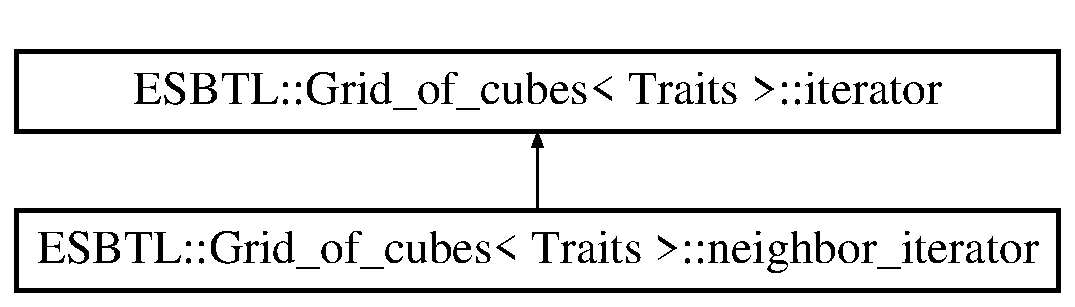
\includegraphics[height=2.000000cm]{classESBTL_1_1Grid__of__cubes_1_1iterator}
\end{center}
\end{figure}
\subsection*{Public Member Functions}
\begin{DoxyCompactItemize}
\item 
\hyperlink{classESBTL_1_1Grid__of__cubes_1_1iterator_a5001cc15c0fa9403d6918232e4b1615e}{iterator} ()
\item 
\hyperlink{classESBTL_1_1Grid__of__cubes_1_1iterator_aed5f716a67875af48b15bad0d34b7b8d}{iterator} (const \hyperlink{structESBTL_1_1Grid__of__cubes_ad55c84346bab961e08d95e494551d07d}{Cube\+\_\+coordinates} \&C)
\item 
\hyperlink{classESBTL_1_1Grid__of__cubes_1_1iterator_abb5f0f7eb3481c3e8b6bb6d4c9ea685d}{iterator} (\hyperlink{structESBTL_1_1Grid__of__cubes}{Grid\+\_\+of\+\_\+cubes} $\ast$Grd)
\item 
\hyperlink{classESBTL_1_1Grid__of__cubes_1_1iterator_a03419d0f3256eecdd89560a8e0bbea8c}{iterator} (\hyperlink{structESBTL_1_1Grid__of__cubes}{Grid\+\_\+of\+\_\+cubes} $\ast$Grd, const \hyperlink{structESBTL_1_1Grid__of__cubes_ad55c84346bab961e08d95e494551d07d}{Cube\+\_\+coordinates} \&C)
\item 
\hyperlink{classESBTL_1_1Grid__of__cubes_1_1iterator}{iterator} \& \hyperlink{classESBTL_1_1Grid__of__cubes_1_1iterator_a276b1498dca08866f128292f6505609c}{operator++} ()
\item 
\hyperlink{structESBTL_1_1Grid__of__cubes_1_1Cube__unit}{Cube\+\_\+unit} \& \hyperlink{classESBTL_1_1Grid__of__cubes_1_1iterator_aa3017ff39fe5fbc9658bd998297da766}{operator$\ast$} ()
\item 
\hyperlink{structESBTL_1_1Grid__of__cubes_1_1Cube__unit}{Cube\+\_\+unit} $\ast$ \hyperlink{classESBTL_1_1Grid__of__cubes_1_1iterator_a6244a3042ab6bc853b3cf9b5d1b55969}{operator-\/$>$} ()
\item 
bool \hyperlink{classESBTL_1_1Grid__of__cubes_1_1iterator_a94ea652fb193dcb86f982a42ebf6d0cb}{operator==} (const \hyperlink{classESBTL_1_1Grid__of__cubes_1_1iterator}{iterator} \&it)
\item 
bool \hyperlink{classESBTL_1_1Grid__of__cubes_1_1iterator_a4253cb445b2ab323b8db82336b6c554f}{operator!=} (const \hyperlink{classESBTL_1_1Grid__of__cubes_1_1iterator}{iterator} \&it)
\end{DoxyCompactItemize}
\subsection*{Protected Member Functions}
\begin{DoxyCompactItemize}
\item 
\hyperlink{structESBTL_1_1Grid__of__cubes_ad55c84346bab961e08d95e494551d07d}{Cube\+\_\+coordinates} \hyperlink{classESBTL_1_1Grid__of__cubes_1_1iterator_a8d881de503568216ba8f4ebef6b144f2}{get\+\_\+next} ()
\end{DoxyCompactItemize}
\subsection*{Protected Attributes}
\begin{DoxyCompactItemize}
\item 
\hyperlink{structESBTL_1_1Grid__of__cubes_ad55c84346bab961e08d95e494551d07d}{Cube\+\_\+coordinates} \hyperlink{classESBTL_1_1Grid__of__cubes_1_1iterator_ab757f8b4d627babbf64ecc13a6de06f6}{current}
\item 
\hyperlink{structESBTL_1_1Grid__of__cubes}{Grid\+\_\+of\+\_\+cubes} $\ast$ \hyperlink{classESBTL_1_1Grid__of__cubes_1_1iterator_a492fb31fc0f9f1f7f61914a45bb7ed2e}{grid\+\_\+ptr}
\end{DoxyCompactItemize}
\subsection*{Friends}
\begin{DoxyCompactItemize}
\item 
class \hyperlink{classESBTL_1_1Grid__of__cubes_1_1iterator_a138d76a0aaa6fd7b0cbba3acb1474405}{Grid\+\_\+of\+\_\+cubes$<$ Traits $>$\+::object\+\_\+iterator}
\item 
void \hyperlink{classESBTL_1_1Grid__of__cubes_1_1iterator_a34522cc0511a0818c99ebcd4d1f010ec}{Grid\+\_\+of\+\_\+cubes} (const \hyperlink{classESBTL_1_1Grid__of__cubes_1_1object__iterator}{object\+\_\+iterator} \&it)
\end{DoxyCompactItemize}


\subsection{Constructor \& Destructor Documentation}
\mbox{\Hypertarget{classESBTL_1_1Grid__of__cubes_1_1iterator_a5001cc15c0fa9403d6918232e4b1615e}\label{classESBTL_1_1Grid__of__cubes_1_1iterator_a5001cc15c0fa9403d6918232e4b1615e}} 
\index{E\+S\+B\+T\+L\+::\+Grid\+\_\+of\+\_\+cubes\+::iterator@{E\+S\+B\+T\+L\+::\+Grid\+\_\+of\+\_\+cubes\+::iterator}!iterator@{iterator}}
\index{iterator@{iterator}!E\+S\+B\+T\+L\+::\+Grid\+\_\+of\+\_\+cubes\+::iterator@{E\+S\+B\+T\+L\+::\+Grid\+\_\+of\+\_\+cubes\+::iterator}}
\subsubsection{\texorpdfstring{iterator()}{iterator()}\hspace{0.1cm}{\footnotesize\ttfamily [1/4]}}
{\footnotesize\ttfamily template$<$class Traits $>$ \\
\hyperlink{structESBTL_1_1Grid__of__cubes}{E\+S\+B\+T\+L\+::\+Grid\+\_\+of\+\_\+cubes}$<$ Traits $>$\+::iterator\+::iterator (\begin{DoxyParamCaption}{ }\end{DoxyParamCaption})\hspace{0.3cm}{\ttfamily [inline]}}

\mbox{\Hypertarget{classESBTL_1_1Grid__of__cubes_1_1iterator_aed5f716a67875af48b15bad0d34b7b8d}\label{classESBTL_1_1Grid__of__cubes_1_1iterator_aed5f716a67875af48b15bad0d34b7b8d}} 
\index{E\+S\+B\+T\+L\+::\+Grid\+\_\+of\+\_\+cubes\+::iterator@{E\+S\+B\+T\+L\+::\+Grid\+\_\+of\+\_\+cubes\+::iterator}!iterator@{iterator}}
\index{iterator@{iterator}!E\+S\+B\+T\+L\+::\+Grid\+\_\+of\+\_\+cubes\+::iterator@{E\+S\+B\+T\+L\+::\+Grid\+\_\+of\+\_\+cubes\+::iterator}}
\subsubsection{\texorpdfstring{iterator()}{iterator()}\hspace{0.1cm}{\footnotesize\ttfamily [2/4]}}
{\footnotesize\ttfamily template$<$class Traits $>$ \\
\hyperlink{structESBTL_1_1Grid__of__cubes}{E\+S\+B\+T\+L\+::\+Grid\+\_\+of\+\_\+cubes}$<$ Traits $>$\+::iterator\+::iterator (\begin{DoxyParamCaption}\item[{const \hyperlink{structESBTL_1_1Grid__of__cubes_ad55c84346bab961e08d95e494551d07d}{Cube\+\_\+coordinates} \&}]{C }\end{DoxyParamCaption})\hspace{0.3cm}{\ttfamily [inline]}}

\mbox{\Hypertarget{classESBTL_1_1Grid__of__cubes_1_1iterator_abb5f0f7eb3481c3e8b6bb6d4c9ea685d}\label{classESBTL_1_1Grid__of__cubes_1_1iterator_abb5f0f7eb3481c3e8b6bb6d4c9ea685d}} 
\index{E\+S\+B\+T\+L\+::\+Grid\+\_\+of\+\_\+cubes\+::iterator@{E\+S\+B\+T\+L\+::\+Grid\+\_\+of\+\_\+cubes\+::iterator}!iterator@{iterator}}
\index{iterator@{iterator}!E\+S\+B\+T\+L\+::\+Grid\+\_\+of\+\_\+cubes\+::iterator@{E\+S\+B\+T\+L\+::\+Grid\+\_\+of\+\_\+cubes\+::iterator}}
\subsubsection{\texorpdfstring{iterator()}{iterator()}\hspace{0.1cm}{\footnotesize\ttfamily [3/4]}}
{\footnotesize\ttfamily template$<$class Traits $>$ \\
\hyperlink{structESBTL_1_1Grid__of__cubes}{E\+S\+B\+T\+L\+::\+Grid\+\_\+of\+\_\+cubes}$<$ Traits $>$\+::iterator\+::iterator (\begin{DoxyParamCaption}\item[{\hyperlink{structESBTL_1_1Grid__of__cubes}{Grid\+\_\+of\+\_\+cubes} $\ast$}]{Grd }\end{DoxyParamCaption})\hspace{0.3cm}{\ttfamily [inline]}}

\mbox{\Hypertarget{classESBTL_1_1Grid__of__cubes_1_1iterator_a03419d0f3256eecdd89560a8e0bbea8c}\label{classESBTL_1_1Grid__of__cubes_1_1iterator_a03419d0f3256eecdd89560a8e0bbea8c}} 
\index{E\+S\+B\+T\+L\+::\+Grid\+\_\+of\+\_\+cubes\+::iterator@{E\+S\+B\+T\+L\+::\+Grid\+\_\+of\+\_\+cubes\+::iterator}!iterator@{iterator}}
\index{iterator@{iterator}!E\+S\+B\+T\+L\+::\+Grid\+\_\+of\+\_\+cubes\+::iterator@{E\+S\+B\+T\+L\+::\+Grid\+\_\+of\+\_\+cubes\+::iterator}}
\subsubsection{\texorpdfstring{iterator()}{iterator()}\hspace{0.1cm}{\footnotesize\ttfamily [4/4]}}
{\footnotesize\ttfamily template$<$class Traits $>$ \\
\hyperlink{structESBTL_1_1Grid__of__cubes}{E\+S\+B\+T\+L\+::\+Grid\+\_\+of\+\_\+cubes}$<$ Traits $>$\+::iterator\+::iterator (\begin{DoxyParamCaption}\item[{\hyperlink{structESBTL_1_1Grid__of__cubes}{Grid\+\_\+of\+\_\+cubes} $\ast$}]{Grd,  }\item[{const \hyperlink{structESBTL_1_1Grid__of__cubes_ad55c84346bab961e08d95e494551d07d}{Cube\+\_\+coordinates} \&}]{C }\end{DoxyParamCaption})\hspace{0.3cm}{\ttfamily [inline]}}



\subsection{Member Function Documentation}
\mbox{\Hypertarget{classESBTL_1_1Grid__of__cubes_1_1iterator_a8d881de503568216ba8f4ebef6b144f2}\label{classESBTL_1_1Grid__of__cubes_1_1iterator_a8d881de503568216ba8f4ebef6b144f2}} 
\index{E\+S\+B\+T\+L\+::\+Grid\+\_\+of\+\_\+cubes\+::iterator@{E\+S\+B\+T\+L\+::\+Grid\+\_\+of\+\_\+cubes\+::iterator}!get\+\_\+next@{get\+\_\+next}}
\index{get\+\_\+next@{get\+\_\+next}!E\+S\+B\+T\+L\+::\+Grid\+\_\+of\+\_\+cubes\+::iterator@{E\+S\+B\+T\+L\+::\+Grid\+\_\+of\+\_\+cubes\+::iterator}}
\subsubsection{\texorpdfstring{get\+\_\+next()}{get\_next()}}
{\footnotesize\ttfamily template$<$class Traits $>$ \\
\hyperlink{structESBTL_1_1Grid__of__cubes_ad55c84346bab961e08d95e494551d07d}{Cube\+\_\+coordinates} \hyperlink{structESBTL_1_1Grid__of__cubes}{E\+S\+B\+T\+L\+::\+Grid\+\_\+of\+\_\+cubes}$<$ Traits $>$\+::iterator\+::get\+\_\+next (\begin{DoxyParamCaption}{ }\end{DoxyParamCaption})\hspace{0.3cm}{\ttfamily [inline]}, {\ttfamily [protected]}}

\mbox{\Hypertarget{classESBTL_1_1Grid__of__cubes_1_1iterator_a4253cb445b2ab323b8db82336b6c554f}\label{classESBTL_1_1Grid__of__cubes_1_1iterator_a4253cb445b2ab323b8db82336b6c554f}} 
\index{E\+S\+B\+T\+L\+::\+Grid\+\_\+of\+\_\+cubes\+::iterator@{E\+S\+B\+T\+L\+::\+Grid\+\_\+of\+\_\+cubes\+::iterator}!operator"!=@{operator"!=}}
\index{operator"!=@{operator"!=}!E\+S\+B\+T\+L\+::\+Grid\+\_\+of\+\_\+cubes\+::iterator@{E\+S\+B\+T\+L\+::\+Grid\+\_\+of\+\_\+cubes\+::iterator}}
\subsubsection{\texorpdfstring{operator"!=()}{operator!=()}}
{\footnotesize\ttfamily template$<$class Traits $>$ \\
bool \hyperlink{structESBTL_1_1Grid__of__cubes}{E\+S\+B\+T\+L\+::\+Grid\+\_\+of\+\_\+cubes}$<$ Traits $>$\+::iterator\+::operator!= (\begin{DoxyParamCaption}\item[{const \hyperlink{classESBTL_1_1Grid__of__cubes_1_1iterator}{iterator} \&}]{it }\end{DoxyParamCaption})\hspace{0.3cm}{\ttfamily [inline]}}

\mbox{\Hypertarget{classESBTL_1_1Grid__of__cubes_1_1iterator_aa3017ff39fe5fbc9658bd998297da766}\label{classESBTL_1_1Grid__of__cubes_1_1iterator_aa3017ff39fe5fbc9658bd998297da766}} 
\index{E\+S\+B\+T\+L\+::\+Grid\+\_\+of\+\_\+cubes\+::iterator@{E\+S\+B\+T\+L\+::\+Grid\+\_\+of\+\_\+cubes\+::iterator}!operator$\ast$@{operator$\ast$}}
\index{operator$\ast$@{operator$\ast$}!E\+S\+B\+T\+L\+::\+Grid\+\_\+of\+\_\+cubes\+::iterator@{E\+S\+B\+T\+L\+::\+Grid\+\_\+of\+\_\+cubes\+::iterator}}
\subsubsection{\texorpdfstring{operator$\ast$()}{operator*()}}
{\footnotesize\ttfamily template$<$class Traits $>$ \\
\hyperlink{structESBTL_1_1Grid__of__cubes_1_1Cube__unit}{Cube\+\_\+unit}\& \hyperlink{structESBTL_1_1Grid__of__cubes}{E\+S\+B\+T\+L\+::\+Grid\+\_\+of\+\_\+cubes}$<$ Traits $>$\+::iterator\+::operator$\ast$ (\begin{DoxyParamCaption}{ }\end{DoxyParamCaption})\hspace{0.3cm}{\ttfamily [inline]}}

\mbox{\Hypertarget{classESBTL_1_1Grid__of__cubes_1_1iterator_a276b1498dca08866f128292f6505609c}\label{classESBTL_1_1Grid__of__cubes_1_1iterator_a276b1498dca08866f128292f6505609c}} 
\index{E\+S\+B\+T\+L\+::\+Grid\+\_\+of\+\_\+cubes\+::iterator@{E\+S\+B\+T\+L\+::\+Grid\+\_\+of\+\_\+cubes\+::iterator}!operator++@{operator++}}
\index{operator++@{operator++}!E\+S\+B\+T\+L\+::\+Grid\+\_\+of\+\_\+cubes\+::iterator@{E\+S\+B\+T\+L\+::\+Grid\+\_\+of\+\_\+cubes\+::iterator}}
\subsubsection{\texorpdfstring{operator++()}{operator++()}}
{\footnotesize\ttfamily template$<$class Traits $>$ \\
\hyperlink{classESBTL_1_1Grid__of__cubes_1_1iterator}{iterator}\& \hyperlink{structESBTL_1_1Grid__of__cubes}{E\+S\+B\+T\+L\+::\+Grid\+\_\+of\+\_\+cubes}$<$ Traits $>$\+::iterator\+::operator++ (\begin{DoxyParamCaption}{ }\end{DoxyParamCaption})\hspace{0.3cm}{\ttfamily [inline]}}

\mbox{\Hypertarget{classESBTL_1_1Grid__of__cubes_1_1iterator_a6244a3042ab6bc853b3cf9b5d1b55969}\label{classESBTL_1_1Grid__of__cubes_1_1iterator_a6244a3042ab6bc853b3cf9b5d1b55969}} 
\index{E\+S\+B\+T\+L\+::\+Grid\+\_\+of\+\_\+cubes\+::iterator@{E\+S\+B\+T\+L\+::\+Grid\+\_\+of\+\_\+cubes\+::iterator}!operator-\/$>$@{operator-\/$>$}}
\index{operator-\/$>$@{operator-\/$>$}!E\+S\+B\+T\+L\+::\+Grid\+\_\+of\+\_\+cubes\+::iterator@{E\+S\+B\+T\+L\+::\+Grid\+\_\+of\+\_\+cubes\+::iterator}}
\subsubsection{\texorpdfstring{operator-\/$>$()}{operator->()}}
{\footnotesize\ttfamily template$<$class Traits $>$ \\
\hyperlink{structESBTL_1_1Grid__of__cubes_1_1Cube__unit}{Cube\+\_\+unit}$\ast$ \hyperlink{structESBTL_1_1Grid__of__cubes}{E\+S\+B\+T\+L\+::\+Grid\+\_\+of\+\_\+cubes}$<$ Traits $>$\+::iterator\+::operator-\/$>$ (\begin{DoxyParamCaption}{ }\end{DoxyParamCaption})\hspace{0.3cm}{\ttfamily [inline]}}

\mbox{\Hypertarget{classESBTL_1_1Grid__of__cubes_1_1iterator_a94ea652fb193dcb86f982a42ebf6d0cb}\label{classESBTL_1_1Grid__of__cubes_1_1iterator_a94ea652fb193dcb86f982a42ebf6d0cb}} 
\index{E\+S\+B\+T\+L\+::\+Grid\+\_\+of\+\_\+cubes\+::iterator@{E\+S\+B\+T\+L\+::\+Grid\+\_\+of\+\_\+cubes\+::iterator}!operator==@{operator==}}
\index{operator==@{operator==}!E\+S\+B\+T\+L\+::\+Grid\+\_\+of\+\_\+cubes\+::iterator@{E\+S\+B\+T\+L\+::\+Grid\+\_\+of\+\_\+cubes\+::iterator}}
\subsubsection{\texorpdfstring{operator==()}{operator==()}}
{\footnotesize\ttfamily template$<$class Traits $>$ \\
bool \hyperlink{structESBTL_1_1Grid__of__cubes}{E\+S\+B\+T\+L\+::\+Grid\+\_\+of\+\_\+cubes}$<$ Traits $>$\+::iterator\+::operator== (\begin{DoxyParamCaption}\item[{const \hyperlink{classESBTL_1_1Grid__of__cubes_1_1iterator}{iterator} \&}]{it }\end{DoxyParamCaption})\hspace{0.3cm}{\ttfamily [inline]}}



\subsection{Friends And Related Function Documentation}
\mbox{\Hypertarget{classESBTL_1_1Grid__of__cubes_1_1iterator_a34522cc0511a0818c99ebcd4d1f010ec}\label{classESBTL_1_1Grid__of__cubes_1_1iterator_a34522cc0511a0818c99ebcd4d1f010ec}} 
\index{E\+S\+B\+T\+L\+::\+Grid\+\_\+of\+\_\+cubes\+::iterator@{E\+S\+B\+T\+L\+::\+Grid\+\_\+of\+\_\+cubes\+::iterator}!Grid\+\_\+of\+\_\+cubes@{Grid\+\_\+of\+\_\+cubes}}
\index{Grid\+\_\+of\+\_\+cubes@{Grid\+\_\+of\+\_\+cubes}!E\+S\+B\+T\+L\+::\+Grid\+\_\+of\+\_\+cubes\+::iterator@{E\+S\+B\+T\+L\+::\+Grid\+\_\+of\+\_\+cubes\+::iterator}}
\subsubsection{\texorpdfstring{Grid\+\_\+of\+\_\+cubes}{Grid\_of\_cubes}}
{\footnotesize\ttfamily template$<$class Traits $>$ \\
void \hyperlink{structESBTL_1_1Grid__of__cubes}{Grid\+\_\+of\+\_\+cubes} (\begin{DoxyParamCaption}\item[{const \hyperlink{classESBTL_1_1Grid__of__cubes_1_1object__iterator}{object\+\_\+iterator} \&}]{it }\end{DoxyParamCaption})\hspace{0.3cm}{\ttfamily [friend]}}

\mbox{\Hypertarget{classESBTL_1_1Grid__of__cubes_1_1iterator_a138d76a0aaa6fd7b0cbba3acb1474405}\label{classESBTL_1_1Grid__of__cubes_1_1iterator_a138d76a0aaa6fd7b0cbba3acb1474405}} 
\index{E\+S\+B\+T\+L\+::\+Grid\+\_\+of\+\_\+cubes\+::iterator@{E\+S\+B\+T\+L\+::\+Grid\+\_\+of\+\_\+cubes\+::iterator}!Grid\+\_\+of\+\_\+cubes$<$ Traits $>$\+::object\+\_\+iterator@{Grid\+\_\+of\+\_\+cubes$<$ Traits $>$\+::object\+\_\+iterator}}
\index{Grid\+\_\+of\+\_\+cubes$<$ Traits $>$\+::object\+\_\+iterator@{Grid\+\_\+of\+\_\+cubes$<$ Traits $>$\+::object\+\_\+iterator}!E\+S\+B\+T\+L\+::\+Grid\+\_\+of\+\_\+cubes\+::iterator@{E\+S\+B\+T\+L\+::\+Grid\+\_\+of\+\_\+cubes\+::iterator}}
\subsubsection{\texorpdfstring{Grid\+\_\+of\+\_\+cubes$<$ Traits $>$\+::object\+\_\+iterator}{Grid\_of\_cubes< Traits >::object\_iterator}}
{\footnotesize\ttfamily template$<$class Traits $>$ \\
friend class \hyperlink{structESBTL_1_1Grid__of__cubes}{Grid\+\_\+of\+\_\+cubes}$<$ Traits $>$\+::\hyperlink{classESBTL_1_1Grid__of__cubes_1_1object__iterator}{object\+\_\+iterator}\hspace{0.3cm}{\ttfamily [friend]}}



\subsection{Member Data Documentation}
\mbox{\Hypertarget{classESBTL_1_1Grid__of__cubes_1_1iterator_ab757f8b4d627babbf64ecc13a6de06f6}\label{classESBTL_1_1Grid__of__cubes_1_1iterator_ab757f8b4d627babbf64ecc13a6de06f6}} 
\index{E\+S\+B\+T\+L\+::\+Grid\+\_\+of\+\_\+cubes\+::iterator@{E\+S\+B\+T\+L\+::\+Grid\+\_\+of\+\_\+cubes\+::iterator}!current@{current}}
\index{current@{current}!E\+S\+B\+T\+L\+::\+Grid\+\_\+of\+\_\+cubes\+::iterator@{E\+S\+B\+T\+L\+::\+Grid\+\_\+of\+\_\+cubes\+::iterator}}
\subsubsection{\texorpdfstring{current}{current}}
{\footnotesize\ttfamily template$<$class Traits $>$ \\
\hyperlink{structESBTL_1_1Grid__of__cubes_ad55c84346bab961e08d95e494551d07d}{Cube\+\_\+coordinates} \hyperlink{structESBTL_1_1Grid__of__cubes}{E\+S\+B\+T\+L\+::\+Grid\+\_\+of\+\_\+cubes}$<$ Traits $>$\+::iterator\+::current\hspace{0.3cm}{\ttfamily [protected]}}

\mbox{\Hypertarget{classESBTL_1_1Grid__of__cubes_1_1iterator_a492fb31fc0f9f1f7f61914a45bb7ed2e}\label{classESBTL_1_1Grid__of__cubes_1_1iterator_a492fb31fc0f9f1f7f61914a45bb7ed2e}} 
\index{E\+S\+B\+T\+L\+::\+Grid\+\_\+of\+\_\+cubes\+::iterator@{E\+S\+B\+T\+L\+::\+Grid\+\_\+of\+\_\+cubes\+::iterator}!grid\+\_\+ptr@{grid\+\_\+ptr}}
\index{grid\+\_\+ptr@{grid\+\_\+ptr}!E\+S\+B\+T\+L\+::\+Grid\+\_\+of\+\_\+cubes\+::iterator@{E\+S\+B\+T\+L\+::\+Grid\+\_\+of\+\_\+cubes\+::iterator}}
\subsubsection{\texorpdfstring{grid\+\_\+ptr}{grid\_ptr}}
{\footnotesize\ttfamily template$<$class Traits $>$ \\
\hyperlink{structESBTL_1_1Grid__of__cubes}{Grid\+\_\+of\+\_\+cubes}$\ast$ \hyperlink{structESBTL_1_1Grid__of__cubes}{E\+S\+B\+T\+L\+::\+Grid\+\_\+of\+\_\+cubes}$<$ Traits $>$\+::iterator\+::grid\+\_\+ptr\hspace{0.3cm}{\ttfamily [protected]}}



The documentation for this class was generated from the following file\+:\begin{DoxyCompactItemize}
\item 
\hyperlink{grid__of__cubes_8h}{grid\+\_\+of\+\_\+cubes.\+h}\end{DoxyCompactItemize}

\hypertarget{structESBTL_1_1CGAL_1_1Kernel__with__atom}{}\section{E\+S\+B\+TL\+:\+:C\+G\+AL\+:\+:Kernel\+\_\+with\+\_\+atom$<$ F\+T\+\_\+ $>$ Struct Template Reference}
\label{structESBTL_1_1CGAL_1_1Kernel__with__atom}\index{E\+S\+B\+T\+L\+::\+C\+G\+A\+L\+::\+Kernel\+\_\+with\+\_\+atom$<$ F\+T\+\_\+ $>$@{E\+S\+B\+T\+L\+::\+C\+G\+A\+L\+::\+Kernel\+\_\+with\+\_\+atom$<$ F\+T\+\_\+ $>$}}


{\ttfamily \#include $<$E\+P\+I\+C\+\_\+kernel\+\_\+with\+\_\+atom.\+h$>$}

Inheritance diagram for E\+S\+B\+TL\+:\+:C\+G\+AL\+:\+:Kernel\+\_\+with\+\_\+atom$<$ F\+T\+\_\+ $>$\+:\begin{figure}[H]
\begin{center}
\leavevmode
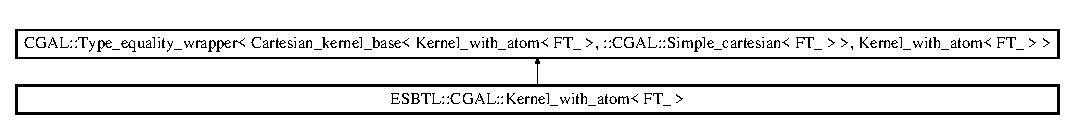
\includegraphics[height=1.293303cm]{structESBTL_1_1CGAL_1_1Kernel__with__atom}
\end{center}
\end{figure}


The documentation for this struct was generated from the following file\+:\begin{DoxyCompactItemize}
\item 
C\+G\+A\+L/\hyperlink{EPIC__kernel__with__atom_8h}{E\+P\+I\+C\+\_\+kernel\+\_\+with\+\_\+atom.\+h}\end{DoxyCompactItemize}

\hypertarget{structESBTL_1_1CGAL_1_1Kernel__with__coarse__atom}{}\section{E\+S\+B\+TL\+:\+:C\+G\+AL\+:\+:Kernel\+\_\+with\+\_\+coarse\+\_\+atom$<$ F\+T\+\_\+ $>$ Struct Template Reference}
\label{structESBTL_1_1CGAL_1_1Kernel__with__coarse__atom}\index{E\+S\+B\+T\+L\+::\+C\+G\+A\+L\+::\+Kernel\+\_\+with\+\_\+coarse\+\_\+atom$<$ F\+T\+\_\+ $>$@{E\+S\+B\+T\+L\+::\+C\+G\+A\+L\+::\+Kernel\+\_\+with\+\_\+coarse\+\_\+atom$<$ F\+T\+\_\+ $>$}}


{\ttfamily \#include $<$E\+P\+I\+C\+\_\+kernel\+\_\+with\+\_\+atom.\+h$>$}

Inheritance diagram for E\+S\+B\+TL\+:\+:C\+G\+AL\+:\+:Kernel\+\_\+with\+\_\+coarse\+\_\+atom$<$ F\+T\+\_\+ $>$\+:\begin{figure}[H]
\begin{center}
\leavevmode
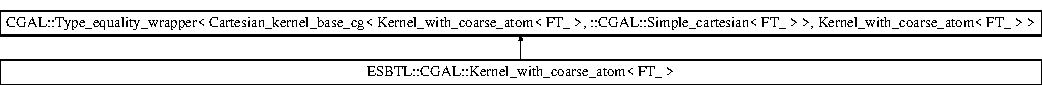
\includegraphics[height=1.144024cm]{structESBTL_1_1CGAL_1_1Kernel__with__coarse__atom}
\end{center}
\end{figure}


The documentation for this struct was generated from the following file\+:\begin{DoxyCompactItemize}
\item 
C\+G\+A\+L/\hyperlink{EPIC__kernel__with__atom_8h}{E\+P\+I\+C\+\_\+kernel\+\_\+with\+\_\+atom.\+h}\end{DoxyCompactItemize}

\hypertarget{classESBTL_1_1PDB_1_1Line__format}{}\section{E\+S\+B\+TL\+:\+:P\+DB\+:\+:Line\+\_\+format$<$ Mandatory\+\_\+fields $>$ Class Template Reference}
\label{classESBTL_1_1PDB_1_1Line__format}\index{E\+S\+B\+T\+L\+::\+P\+D\+B\+::\+Line\+\_\+format$<$ Mandatory\+\_\+fields $>$@{E\+S\+B\+T\+L\+::\+P\+D\+B\+::\+Line\+\_\+format$<$ Mandatory\+\_\+fields $>$}}


{\ttfamily \#include $<$P\+D\+B.\+h$>$}

\subsection*{Public Member Functions}
\begin{DoxyCompactItemize}
\item 
\hyperlink{classESBTL_1_1PDB_1_1Line__format_aaec07c0a69d03b66c4e9e1662f1cadc9}{Line\+\_\+format} (const std\+::string \&line)
\item 
bool \hyperlink{classESBTL_1_1PDB_1_1Line__format_a5985e9f450070463af32eb5438e6f002}{is\+\_\+hetatm} () const
\item 
std\+::string \hyperlink{classESBTL_1_1PDB_1_1Line__format_a3c79f8cc61a87820457d557ae2e6c62c}{get\+\_\+record\+\_\+name} (const std\+::string \&line) const
\item 
int \hyperlink{classESBTL_1_1PDB_1_1Line__format_a04b1c91a27d0fe31b392ab88f4b1764a}{get\+\_\+atom\+\_\+serial\+\_\+number} (const std\+::string \&line) const
\item 
std\+::string \hyperlink{classESBTL_1_1PDB_1_1Line__format_a15c2f8308e18fc058dd7f3a8697ee34a}{get\+\_\+atom\+\_\+name} (const std\+::string \&line) const
\item 
char \hyperlink{classESBTL_1_1PDB_1_1Line__format_a6e389e51c1fc77585024b0cf9f2f4b66}{get\+\_\+alternate\+\_\+location} (const std\+::string \&line) const
\item 
std\+::string \hyperlink{classESBTL_1_1PDB_1_1Line__format_ab0d5125e0fbace190c3f7fabb2eb43e5}{get\+\_\+residue\+\_\+name} (const std\+::string \&line) const
\item 
char \hyperlink{classESBTL_1_1PDB_1_1Line__format_a2db4604a71b9299ec3696d46d1a159bc}{get\+\_\+chain\+\_\+identifier} (const std\+::string \&line) const
\item 
int \hyperlink{classESBTL_1_1PDB_1_1Line__format_a942dc2b1288d12b5a9b5e49ce4eb0371}{get\+\_\+residue\+\_\+sequence\+\_\+number} (const std\+::string \&line) const
\item 
char \hyperlink{classESBTL_1_1PDB_1_1Line__format_a13303838446368779d4b391ba130dcba}{get\+\_\+insertion\+\_\+code} (const std\+::string \&line) const
\item 
double \hyperlink{classESBTL_1_1PDB_1_1Line__format_afe06d4e9bcb00c28d4c4a7ba975d6f0b}{get\+\_\+x} (const std\+::string \&line) const
\item 
double \hyperlink{classESBTL_1_1PDB_1_1Line__format_a48f80ae039ee691802faa980fecb4476}{get\+\_\+y} (const std\+::string \&line) const
\item 
double \hyperlink{classESBTL_1_1PDB_1_1Line__format_a7d7e983d438a17bcd8a799baf6c06ab9}{get\+\_\+z} (const std\+::string \&line) const
\item 
double \hyperlink{classESBTL_1_1PDB_1_1Line__format_a7c2498989dd637f008a1719adb9b44b9}{get\+\_\+occupancy} (const std\+::string \&line) const
\item 
double \hyperlink{classESBTL_1_1PDB_1_1Line__format_afb1db7866fc6f7cc603ed5a9836100ad}{get\+\_\+temperature\+\_\+factor} (const std\+::string \&line) const
\item 
std\+::string \hyperlink{classESBTL_1_1PDB_1_1Line__format_ad38fda5e9c5d68d7da40356119f8537e}{get\+\_\+element} (const std\+::string \&line) const
\item 
std\+::string \hyperlink{classESBTL_1_1PDB_1_1Line__format_ada983c443ea270cc31d9337121ca4e58}{get\+\_\+charge\+\_\+str} (const std\+::string \&line) const
\item 
int \hyperlink{classESBTL_1_1PDB_1_1Line__format_a314acf4e8c390b306beb7fd917e0da31}{get\+\_\+charge} (const std\+::string \&line) const
\item 
int \hyperlink{classESBTL_1_1PDB_1_1Line__format_aa489ba8d76c6f289103da0466ce84e23}{get\+\_\+model\+\_\+number} (const std\+::string \&line) const
\item 
\hyperlink{namespaceESBTL_1_1PDB_a6f11e88f706f51afbe97230641a469b7}{P\+D\+B\+::\+Record\+\_\+type} \hyperlink{classESBTL_1_1PDB_1_1Line__format_ae266a9259dbd80a17d82e0dd42852fa3}{record\+\_\+type} () const
\end{DoxyCompactItemize}


\subsection{Detailed Description}
\subsubsection*{template$<$class Mandatory\+\_\+fields = Mandatory\+\_\+fields\+\_\+default$>$\newline
class E\+S\+B\+T\+L\+::\+P\+D\+B\+::\+Line\+\_\+format$<$ Mandatory\+\_\+fields $>$}

Helper class handle to extract fields from line of a \hyperlink{namespaceESBTL_1_1PDB}{P\+DB} file. 
\begin{DoxyTemplParams}{Template Parameters}
{\em Mandatory\+\_\+fields} & is a class indicating which fields are mandatory (see \hyperlink{structESBTL_1_1PDB_1_1Mandatory__fields__default}{E\+S\+B\+T\+L\+::\+P\+D\+B\+::\+Mandatory\+\_\+fields\+\_\+default} for requirements). \\
\hline
\end{DoxyTemplParams}


\subsection{Constructor \& Destructor Documentation}
\mbox{\Hypertarget{classESBTL_1_1PDB_1_1Line__format_aaec07c0a69d03b66c4e9e1662f1cadc9}\label{classESBTL_1_1PDB_1_1Line__format_aaec07c0a69d03b66c4e9e1662f1cadc9}} 
\index{E\+S\+B\+T\+L\+::\+P\+D\+B\+::\+Line\+\_\+format@{E\+S\+B\+T\+L\+::\+P\+D\+B\+::\+Line\+\_\+format}!Line\+\_\+format@{Line\+\_\+format}}
\index{Line\+\_\+format@{Line\+\_\+format}!E\+S\+B\+T\+L\+::\+P\+D\+B\+::\+Line\+\_\+format@{E\+S\+B\+T\+L\+::\+P\+D\+B\+::\+Line\+\_\+format}}
\subsubsection{\texorpdfstring{Line\+\_\+format()}{Line\_format()}}
{\footnotesize\ttfamily template$<$class Mandatory\+\_\+fields  = Mandatory\+\_\+fields\+\_\+default$>$ \\
\hyperlink{classESBTL_1_1PDB_1_1Line__format}{E\+S\+B\+T\+L\+::\+P\+D\+B\+::\+Line\+\_\+format}$<$ Mandatory\+\_\+fields $>$\+::\hyperlink{classESBTL_1_1PDB_1_1Line__format}{Line\+\_\+format} (\begin{DoxyParamCaption}\item[{const std\+::string \&}]{line }\end{DoxyParamCaption})\hspace{0.3cm}{\ttfamily [inline]}}

Constructor. 
\begin{DoxyParams}{Parameters}
{\em line} & is a line of a \hyperlink{namespaceESBTL_1_1PDB}{P\+DB} file. \\
\hline
\end{DoxyParams}


\subsection{Member Function Documentation}
\mbox{\Hypertarget{classESBTL_1_1PDB_1_1Line__format_a6e389e51c1fc77585024b0cf9f2f4b66}\label{classESBTL_1_1PDB_1_1Line__format_a6e389e51c1fc77585024b0cf9f2f4b66}} 
\index{E\+S\+B\+T\+L\+::\+P\+D\+B\+::\+Line\+\_\+format@{E\+S\+B\+T\+L\+::\+P\+D\+B\+::\+Line\+\_\+format}!get\+\_\+alternate\+\_\+location@{get\+\_\+alternate\+\_\+location}}
\index{get\+\_\+alternate\+\_\+location@{get\+\_\+alternate\+\_\+location}!E\+S\+B\+T\+L\+::\+P\+D\+B\+::\+Line\+\_\+format@{E\+S\+B\+T\+L\+::\+P\+D\+B\+::\+Line\+\_\+format}}
\subsubsection{\texorpdfstring{get\+\_\+alternate\+\_\+location()}{get\_alternate\_location()}}
{\footnotesize\ttfamily template$<$class Mandatory\+\_\+fields  = Mandatory\+\_\+fields\+\_\+default$>$ \\
char \hyperlink{classESBTL_1_1PDB_1_1Line__format}{E\+S\+B\+T\+L\+::\+P\+D\+B\+::\+Line\+\_\+format}$<$ Mandatory\+\_\+fields $>$\+::get\+\_\+alternate\+\_\+location (\begin{DoxyParamCaption}\item[{const std\+::string \&}]{line }\end{DoxyParamCaption}) const\hspace{0.3cm}{\ttfamily [inline]}}

\mbox{\Hypertarget{classESBTL_1_1PDB_1_1Line__format_a15c2f8308e18fc058dd7f3a8697ee34a}\label{classESBTL_1_1PDB_1_1Line__format_a15c2f8308e18fc058dd7f3a8697ee34a}} 
\index{E\+S\+B\+T\+L\+::\+P\+D\+B\+::\+Line\+\_\+format@{E\+S\+B\+T\+L\+::\+P\+D\+B\+::\+Line\+\_\+format}!get\+\_\+atom\+\_\+name@{get\+\_\+atom\+\_\+name}}
\index{get\+\_\+atom\+\_\+name@{get\+\_\+atom\+\_\+name}!E\+S\+B\+T\+L\+::\+P\+D\+B\+::\+Line\+\_\+format@{E\+S\+B\+T\+L\+::\+P\+D\+B\+::\+Line\+\_\+format}}
\subsubsection{\texorpdfstring{get\+\_\+atom\+\_\+name()}{get\_atom\_name()}}
{\footnotesize\ttfamily template$<$class Mandatory\+\_\+fields  = Mandatory\+\_\+fields\+\_\+default$>$ \\
std\+::string \hyperlink{classESBTL_1_1PDB_1_1Line__format}{E\+S\+B\+T\+L\+::\+P\+D\+B\+::\+Line\+\_\+format}$<$ Mandatory\+\_\+fields $>$\+::get\+\_\+atom\+\_\+name (\begin{DoxyParamCaption}\item[{const std\+::string \&}]{line }\end{DoxyParamCaption}) const\hspace{0.3cm}{\ttfamily [inline]}}

\mbox{\Hypertarget{classESBTL_1_1PDB_1_1Line__format_a04b1c91a27d0fe31b392ab88f4b1764a}\label{classESBTL_1_1PDB_1_1Line__format_a04b1c91a27d0fe31b392ab88f4b1764a}} 
\index{E\+S\+B\+T\+L\+::\+P\+D\+B\+::\+Line\+\_\+format@{E\+S\+B\+T\+L\+::\+P\+D\+B\+::\+Line\+\_\+format}!get\+\_\+atom\+\_\+serial\+\_\+number@{get\+\_\+atom\+\_\+serial\+\_\+number}}
\index{get\+\_\+atom\+\_\+serial\+\_\+number@{get\+\_\+atom\+\_\+serial\+\_\+number}!E\+S\+B\+T\+L\+::\+P\+D\+B\+::\+Line\+\_\+format@{E\+S\+B\+T\+L\+::\+P\+D\+B\+::\+Line\+\_\+format}}
\subsubsection{\texorpdfstring{get\+\_\+atom\+\_\+serial\+\_\+number()}{get\_atom\_serial\_number()}}
{\footnotesize\ttfamily template$<$class Mandatory\+\_\+fields  = Mandatory\+\_\+fields\+\_\+default$>$ \\
int \hyperlink{classESBTL_1_1PDB_1_1Line__format}{E\+S\+B\+T\+L\+::\+P\+D\+B\+::\+Line\+\_\+format}$<$ Mandatory\+\_\+fields $>$\+::get\+\_\+atom\+\_\+serial\+\_\+number (\begin{DoxyParamCaption}\item[{const std\+::string \&}]{line }\end{DoxyParamCaption}) const\hspace{0.3cm}{\ttfamily [inline]}}

\mbox{\Hypertarget{classESBTL_1_1PDB_1_1Line__format_a2db4604a71b9299ec3696d46d1a159bc}\label{classESBTL_1_1PDB_1_1Line__format_a2db4604a71b9299ec3696d46d1a159bc}} 
\index{E\+S\+B\+T\+L\+::\+P\+D\+B\+::\+Line\+\_\+format@{E\+S\+B\+T\+L\+::\+P\+D\+B\+::\+Line\+\_\+format}!get\+\_\+chain\+\_\+identifier@{get\+\_\+chain\+\_\+identifier}}
\index{get\+\_\+chain\+\_\+identifier@{get\+\_\+chain\+\_\+identifier}!E\+S\+B\+T\+L\+::\+P\+D\+B\+::\+Line\+\_\+format@{E\+S\+B\+T\+L\+::\+P\+D\+B\+::\+Line\+\_\+format}}
\subsubsection{\texorpdfstring{get\+\_\+chain\+\_\+identifier()}{get\_chain\_identifier()}}
{\footnotesize\ttfamily template$<$class Mandatory\+\_\+fields  = Mandatory\+\_\+fields\+\_\+default$>$ \\
char \hyperlink{classESBTL_1_1PDB_1_1Line__format}{E\+S\+B\+T\+L\+::\+P\+D\+B\+::\+Line\+\_\+format}$<$ Mandatory\+\_\+fields $>$\+::get\+\_\+chain\+\_\+identifier (\begin{DoxyParamCaption}\item[{const std\+::string \&}]{line }\end{DoxyParamCaption}) const\hspace{0.3cm}{\ttfamily [inline]}}

\mbox{\Hypertarget{classESBTL_1_1PDB_1_1Line__format_a314acf4e8c390b306beb7fd917e0da31}\label{classESBTL_1_1PDB_1_1Line__format_a314acf4e8c390b306beb7fd917e0da31}} 
\index{E\+S\+B\+T\+L\+::\+P\+D\+B\+::\+Line\+\_\+format@{E\+S\+B\+T\+L\+::\+P\+D\+B\+::\+Line\+\_\+format}!get\+\_\+charge@{get\+\_\+charge}}
\index{get\+\_\+charge@{get\+\_\+charge}!E\+S\+B\+T\+L\+::\+P\+D\+B\+::\+Line\+\_\+format@{E\+S\+B\+T\+L\+::\+P\+D\+B\+::\+Line\+\_\+format}}
\subsubsection{\texorpdfstring{get\+\_\+charge()}{get\_charge()}}
{\footnotesize\ttfamily template$<$class Mandatory\+\_\+fields  = Mandatory\+\_\+fields\+\_\+default$>$ \\
int \hyperlink{classESBTL_1_1PDB_1_1Line__format}{E\+S\+B\+T\+L\+::\+P\+D\+B\+::\+Line\+\_\+format}$<$ Mandatory\+\_\+fields $>$\+::get\+\_\+charge (\begin{DoxyParamCaption}\item[{const std\+::string \&}]{line }\end{DoxyParamCaption}) const\hspace{0.3cm}{\ttfamily [inline]}}

extract the field charge as an integer. \mbox{\Hypertarget{classESBTL_1_1PDB_1_1Line__format_ada983c443ea270cc31d9337121ca4e58}\label{classESBTL_1_1PDB_1_1Line__format_ada983c443ea270cc31d9337121ca4e58}} 
\index{E\+S\+B\+T\+L\+::\+P\+D\+B\+::\+Line\+\_\+format@{E\+S\+B\+T\+L\+::\+P\+D\+B\+::\+Line\+\_\+format}!get\+\_\+charge\+\_\+str@{get\+\_\+charge\+\_\+str}}
\index{get\+\_\+charge\+\_\+str@{get\+\_\+charge\+\_\+str}!E\+S\+B\+T\+L\+::\+P\+D\+B\+::\+Line\+\_\+format@{E\+S\+B\+T\+L\+::\+P\+D\+B\+::\+Line\+\_\+format}}
\subsubsection{\texorpdfstring{get\+\_\+charge\+\_\+str()}{get\_charge\_str()}}
{\footnotesize\ttfamily template$<$class Mandatory\+\_\+fields  = Mandatory\+\_\+fields\+\_\+default$>$ \\
std\+::string \hyperlink{classESBTL_1_1PDB_1_1Line__format}{E\+S\+B\+T\+L\+::\+P\+D\+B\+::\+Line\+\_\+format}$<$ Mandatory\+\_\+fields $>$\+::get\+\_\+charge\+\_\+str (\begin{DoxyParamCaption}\item[{const std\+::string \&}]{line }\end{DoxyParamCaption}) const\hspace{0.3cm}{\ttfamily [inline]}}

extract the field charge as a string. \mbox{\Hypertarget{classESBTL_1_1PDB_1_1Line__format_ad38fda5e9c5d68d7da40356119f8537e}\label{classESBTL_1_1PDB_1_1Line__format_ad38fda5e9c5d68d7da40356119f8537e}} 
\index{E\+S\+B\+T\+L\+::\+P\+D\+B\+::\+Line\+\_\+format@{E\+S\+B\+T\+L\+::\+P\+D\+B\+::\+Line\+\_\+format}!get\+\_\+element@{get\+\_\+element}}
\index{get\+\_\+element@{get\+\_\+element}!E\+S\+B\+T\+L\+::\+P\+D\+B\+::\+Line\+\_\+format@{E\+S\+B\+T\+L\+::\+P\+D\+B\+::\+Line\+\_\+format}}
\subsubsection{\texorpdfstring{get\+\_\+element()}{get\_element()}}
{\footnotesize\ttfamily template$<$class Mandatory\+\_\+fields  = Mandatory\+\_\+fields\+\_\+default$>$ \\
std\+::string \hyperlink{classESBTL_1_1PDB_1_1Line__format}{E\+S\+B\+T\+L\+::\+P\+D\+B\+::\+Line\+\_\+format}$<$ Mandatory\+\_\+fields $>$\+::get\+\_\+element (\begin{DoxyParamCaption}\item[{const std\+::string \&}]{line }\end{DoxyParamCaption}) const\hspace{0.3cm}{\ttfamily [inline]}}

\mbox{\Hypertarget{classESBTL_1_1PDB_1_1Line__format_a13303838446368779d4b391ba130dcba}\label{classESBTL_1_1PDB_1_1Line__format_a13303838446368779d4b391ba130dcba}} 
\index{E\+S\+B\+T\+L\+::\+P\+D\+B\+::\+Line\+\_\+format@{E\+S\+B\+T\+L\+::\+P\+D\+B\+::\+Line\+\_\+format}!get\+\_\+insertion\+\_\+code@{get\+\_\+insertion\+\_\+code}}
\index{get\+\_\+insertion\+\_\+code@{get\+\_\+insertion\+\_\+code}!E\+S\+B\+T\+L\+::\+P\+D\+B\+::\+Line\+\_\+format@{E\+S\+B\+T\+L\+::\+P\+D\+B\+::\+Line\+\_\+format}}
\subsubsection{\texorpdfstring{get\+\_\+insertion\+\_\+code()}{get\_insertion\_code()}}
{\footnotesize\ttfamily template$<$class Mandatory\+\_\+fields  = Mandatory\+\_\+fields\+\_\+default$>$ \\
char \hyperlink{classESBTL_1_1PDB_1_1Line__format}{E\+S\+B\+T\+L\+::\+P\+D\+B\+::\+Line\+\_\+format}$<$ Mandatory\+\_\+fields $>$\+::get\+\_\+insertion\+\_\+code (\begin{DoxyParamCaption}\item[{const std\+::string \&}]{line }\end{DoxyParamCaption}) const\hspace{0.3cm}{\ttfamily [inline]}}

\mbox{\Hypertarget{classESBTL_1_1PDB_1_1Line__format_aa489ba8d76c6f289103da0466ce84e23}\label{classESBTL_1_1PDB_1_1Line__format_aa489ba8d76c6f289103da0466ce84e23}} 
\index{E\+S\+B\+T\+L\+::\+P\+D\+B\+::\+Line\+\_\+format@{E\+S\+B\+T\+L\+::\+P\+D\+B\+::\+Line\+\_\+format}!get\+\_\+model\+\_\+number@{get\+\_\+model\+\_\+number}}
\index{get\+\_\+model\+\_\+number@{get\+\_\+model\+\_\+number}!E\+S\+B\+T\+L\+::\+P\+D\+B\+::\+Line\+\_\+format@{E\+S\+B\+T\+L\+::\+P\+D\+B\+::\+Line\+\_\+format}}
\subsubsection{\texorpdfstring{get\+\_\+model\+\_\+number()}{get\_model\_number()}}
{\footnotesize\ttfamily template$<$class Mandatory\+\_\+fields  = Mandatory\+\_\+fields\+\_\+default$>$ \\
int \hyperlink{classESBTL_1_1PDB_1_1Line__format}{E\+S\+B\+T\+L\+::\+P\+D\+B\+::\+Line\+\_\+format}$<$ Mandatory\+\_\+fields $>$\+::get\+\_\+model\+\_\+number (\begin{DoxyParamCaption}\item[{const std\+::string \&}]{line }\end{DoxyParamCaption}) const\hspace{0.3cm}{\ttfamily [inline]}}

\mbox{\Hypertarget{classESBTL_1_1PDB_1_1Line__format_a7c2498989dd637f008a1719adb9b44b9}\label{classESBTL_1_1PDB_1_1Line__format_a7c2498989dd637f008a1719adb9b44b9}} 
\index{E\+S\+B\+T\+L\+::\+P\+D\+B\+::\+Line\+\_\+format@{E\+S\+B\+T\+L\+::\+P\+D\+B\+::\+Line\+\_\+format}!get\+\_\+occupancy@{get\+\_\+occupancy}}
\index{get\+\_\+occupancy@{get\+\_\+occupancy}!E\+S\+B\+T\+L\+::\+P\+D\+B\+::\+Line\+\_\+format@{E\+S\+B\+T\+L\+::\+P\+D\+B\+::\+Line\+\_\+format}}
\subsubsection{\texorpdfstring{get\+\_\+occupancy()}{get\_occupancy()}}
{\footnotesize\ttfamily template$<$class Mandatory\+\_\+fields  = Mandatory\+\_\+fields\+\_\+default$>$ \\
double \hyperlink{classESBTL_1_1PDB_1_1Line__format}{E\+S\+B\+T\+L\+::\+P\+D\+B\+::\+Line\+\_\+format}$<$ Mandatory\+\_\+fields $>$\+::get\+\_\+occupancy (\begin{DoxyParamCaption}\item[{const std\+::string \&}]{line }\end{DoxyParamCaption}) const\hspace{0.3cm}{\ttfamily [inline]}}

\mbox{\Hypertarget{classESBTL_1_1PDB_1_1Line__format_a3c79f8cc61a87820457d557ae2e6c62c}\label{classESBTL_1_1PDB_1_1Line__format_a3c79f8cc61a87820457d557ae2e6c62c}} 
\index{E\+S\+B\+T\+L\+::\+P\+D\+B\+::\+Line\+\_\+format@{E\+S\+B\+T\+L\+::\+P\+D\+B\+::\+Line\+\_\+format}!get\+\_\+record\+\_\+name@{get\+\_\+record\+\_\+name}}
\index{get\+\_\+record\+\_\+name@{get\+\_\+record\+\_\+name}!E\+S\+B\+T\+L\+::\+P\+D\+B\+::\+Line\+\_\+format@{E\+S\+B\+T\+L\+::\+P\+D\+B\+::\+Line\+\_\+format}}
\subsubsection{\texorpdfstring{get\+\_\+record\+\_\+name()}{get\_record\_name()}}
{\footnotesize\ttfamily template$<$class Mandatory\+\_\+fields  = Mandatory\+\_\+fields\+\_\+default$>$ \\
std\+::string \hyperlink{classESBTL_1_1PDB_1_1Line__format}{E\+S\+B\+T\+L\+::\+P\+D\+B\+::\+Line\+\_\+format}$<$ Mandatory\+\_\+fields $>$\+::get\+\_\+record\+\_\+name (\begin{DoxyParamCaption}\item[{const std\+::string \&}]{line }\end{DoxyParamCaption}) const\hspace{0.3cm}{\ttfamily [inline]}}

\mbox{\Hypertarget{classESBTL_1_1PDB_1_1Line__format_ab0d5125e0fbace190c3f7fabb2eb43e5}\label{classESBTL_1_1PDB_1_1Line__format_ab0d5125e0fbace190c3f7fabb2eb43e5}} 
\index{E\+S\+B\+T\+L\+::\+P\+D\+B\+::\+Line\+\_\+format@{E\+S\+B\+T\+L\+::\+P\+D\+B\+::\+Line\+\_\+format}!get\+\_\+residue\+\_\+name@{get\+\_\+residue\+\_\+name}}
\index{get\+\_\+residue\+\_\+name@{get\+\_\+residue\+\_\+name}!E\+S\+B\+T\+L\+::\+P\+D\+B\+::\+Line\+\_\+format@{E\+S\+B\+T\+L\+::\+P\+D\+B\+::\+Line\+\_\+format}}
\subsubsection{\texorpdfstring{get\+\_\+residue\+\_\+name()}{get\_residue\_name()}}
{\footnotesize\ttfamily template$<$class Mandatory\+\_\+fields  = Mandatory\+\_\+fields\+\_\+default$>$ \\
std\+::string \hyperlink{classESBTL_1_1PDB_1_1Line__format}{E\+S\+B\+T\+L\+::\+P\+D\+B\+::\+Line\+\_\+format}$<$ Mandatory\+\_\+fields $>$\+::get\+\_\+residue\+\_\+name (\begin{DoxyParamCaption}\item[{const std\+::string \&}]{line }\end{DoxyParamCaption}) const\hspace{0.3cm}{\ttfamily [inline]}}

\mbox{\Hypertarget{classESBTL_1_1PDB_1_1Line__format_a942dc2b1288d12b5a9b5e49ce4eb0371}\label{classESBTL_1_1PDB_1_1Line__format_a942dc2b1288d12b5a9b5e49ce4eb0371}} 
\index{E\+S\+B\+T\+L\+::\+P\+D\+B\+::\+Line\+\_\+format@{E\+S\+B\+T\+L\+::\+P\+D\+B\+::\+Line\+\_\+format}!get\+\_\+residue\+\_\+sequence\+\_\+number@{get\+\_\+residue\+\_\+sequence\+\_\+number}}
\index{get\+\_\+residue\+\_\+sequence\+\_\+number@{get\+\_\+residue\+\_\+sequence\+\_\+number}!E\+S\+B\+T\+L\+::\+P\+D\+B\+::\+Line\+\_\+format@{E\+S\+B\+T\+L\+::\+P\+D\+B\+::\+Line\+\_\+format}}
\subsubsection{\texorpdfstring{get\+\_\+residue\+\_\+sequence\+\_\+number()}{get\_residue\_sequence\_number()}}
{\footnotesize\ttfamily template$<$class Mandatory\+\_\+fields  = Mandatory\+\_\+fields\+\_\+default$>$ \\
int \hyperlink{classESBTL_1_1PDB_1_1Line__format}{E\+S\+B\+T\+L\+::\+P\+D\+B\+::\+Line\+\_\+format}$<$ Mandatory\+\_\+fields $>$\+::get\+\_\+residue\+\_\+sequence\+\_\+number (\begin{DoxyParamCaption}\item[{const std\+::string \&}]{line }\end{DoxyParamCaption}) const\hspace{0.3cm}{\ttfamily [inline]}}

\mbox{\Hypertarget{classESBTL_1_1PDB_1_1Line__format_afb1db7866fc6f7cc603ed5a9836100ad}\label{classESBTL_1_1PDB_1_1Line__format_afb1db7866fc6f7cc603ed5a9836100ad}} 
\index{E\+S\+B\+T\+L\+::\+P\+D\+B\+::\+Line\+\_\+format@{E\+S\+B\+T\+L\+::\+P\+D\+B\+::\+Line\+\_\+format}!get\+\_\+temperature\+\_\+factor@{get\+\_\+temperature\+\_\+factor}}
\index{get\+\_\+temperature\+\_\+factor@{get\+\_\+temperature\+\_\+factor}!E\+S\+B\+T\+L\+::\+P\+D\+B\+::\+Line\+\_\+format@{E\+S\+B\+T\+L\+::\+P\+D\+B\+::\+Line\+\_\+format}}
\subsubsection{\texorpdfstring{get\+\_\+temperature\+\_\+factor()}{get\_temperature\_factor()}}
{\footnotesize\ttfamily template$<$class Mandatory\+\_\+fields  = Mandatory\+\_\+fields\+\_\+default$>$ \\
double \hyperlink{classESBTL_1_1PDB_1_1Line__format}{E\+S\+B\+T\+L\+::\+P\+D\+B\+::\+Line\+\_\+format}$<$ Mandatory\+\_\+fields $>$\+::get\+\_\+temperature\+\_\+factor (\begin{DoxyParamCaption}\item[{const std\+::string \&}]{line }\end{DoxyParamCaption}) const\hspace{0.3cm}{\ttfamily [inline]}}

\mbox{\Hypertarget{classESBTL_1_1PDB_1_1Line__format_afe06d4e9bcb00c28d4c4a7ba975d6f0b}\label{classESBTL_1_1PDB_1_1Line__format_afe06d4e9bcb00c28d4c4a7ba975d6f0b}} 
\index{E\+S\+B\+T\+L\+::\+P\+D\+B\+::\+Line\+\_\+format@{E\+S\+B\+T\+L\+::\+P\+D\+B\+::\+Line\+\_\+format}!get\+\_\+x@{get\+\_\+x}}
\index{get\+\_\+x@{get\+\_\+x}!E\+S\+B\+T\+L\+::\+P\+D\+B\+::\+Line\+\_\+format@{E\+S\+B\+T\+L\+::\+P\+D\+B\+::\+Line\+\_\+format}}
\subsubsection{\texorpdfstring{get\+\_\+x()}{get\_x()}}
{\footnotesize\ttfamily template$<$class Mandatory\+\_\+fields  = Mandatory\+\_\+fields\+\_\+default$>$ \\
double \hyperlink{classESBTL_1_1PDB_1_1Line__format}{E\+S\+B\+T\+L\+::\+P\+D\+B\+::\+Line\+\_\+format}$<$ Mandatory\+\_\+fields $>$\+::get\+\_\+x (\begin{DoxyParamCaption}\item[{const std\+::string \&}]{line }\end{DoxyParamCaption}) const\hspace{0.3cm}{\ttfamily [inline]}}

\mbox{\Hypertarget{classESBTL_1_1PDB_1_1Line__format_a48f80ae039ee691802faa980fecb4476}\label{classESBTL_1_1PDB_1_1Line__format_a48f80ae039ee691802faa980fecb4476}} 
\index{E\+S\+B\+T\+L\+::\+P\+D\+B\+::\+Line\+\_\+format@{E\+S\+B\+T\+L\+::\+P\+D\+B\+::\+Line\+\_\+format}!get\+\_\+y@{get\+\_\+y}}
\index{get\+\_\+y@{get\+\_\+y}!E\+S\+B\+T\+L\+::\+P\+D\+B\+::\+Line\+\_\+format@{E\+S\+B\+T\+L\+::\+P\+D\+B\+::\+Line\+\_\+format}}
\subsubsection{\texorpdfstring{get\+\_\+y()}{get\_y()}}
{\footnotesize\ttfamily template$<$class Mandatory\+\_\+fields  = Mandatory\+\_\+fields\+\_\+default$>$ \\
double \hyperlink{classESBTL_1_1PDB_1_1Line__format}{E\+S\+B\+T\+L\+::\+P\+D\+B\+::\+Line\+\_\+format}$<$ Mandatory\+\_\+fields $>$\+::get\+\_\+y (\begin{DoxyParamCaption}\item[{const std\+::string \&}]{line }\end{DoxyParamCaption}) const\hspace{0.3cm}{\ttfamily [inline]}}

\mbox{\Hypertarget{classESBTL_1_1PDB_1_1Line__format_a7d7e983d438a17bcd8a799baf6c06ab9}\label{classESBTL_1_1PDB_1_1Line__format_a7d7e983d438a17bcd8a799baf6c06ab9}} 
\index{E\+S\+B\+T\+L\+::\+P\+D\+B\+::\+Line\+\_\+format@{E\+S\+B\+T\+L\+::\+P\+D\+B\+::\+Line\+\_\+format}!get\+\_\+z@{get\+\_\+z}}
\index{get\+\_\+z@{get\+\_\+z}!E\+S\+B\+T\+L\+::\+P\+D\+B\+::\+Line\+\_\+format@{E\+S\+B\+T\+L\+::\+P\+D\+B\+::\+Line\+\_\+format}}
\subsubsection{\texorpdfstring{get\+\_\+z()}{get\_z()}}
{\footnotesize\ttfamily template$<$class Mandatory\+\_\+fields  = Mandatory\+\_\+fields\+\_\+default$>$ \\
double \hyperlink{classESBTL_1_1PDB_1_1Line__format}{E\+S\+B\+T\+L\+::\+P\+D\+B\+::\+Line\+\_\+format}$<$ Mandatory\+\_\+fields $>$\+::get\+\_\+z (\begin{DoxyParamCaption}\item[{const std\+::string \&}]{line }\end{DoxyParamCaption}) const\hspace{0.3cm}{\ttfamily [inline]}}

\mbox{\Hypertarget{classESBTL_1_1PDB_1_1Line__format_a5985e9f450070463af32eb5438e6f002}\label{classESBTL_1_1PDB_1_1Line__format_a5985e9f450070463af32eb5438e6f002}} 
\index{E\+S\+B\+T\+L\+::\+P\+D\+B\+::\+Line\+\_\+format@{E\+S\+B\+T\+L\+::\+P\+D\+B\+::\+Line\+\_\+format}!is\+\_\+hetatm@{is\+\_\+hetatm}}
\index{is\+\_\+hetatm@{is\+\_\+hetatm}!E\+S\+B\+T\+L\+::\+P\+D\+B\+::\+Line\+\_\+format@{E\+S\+B\+T\+L\+::\+P\+D\+B\+::\+Line\+\_\+format}}
\subsubsection{\texorpdfstring{is\+\_\+hetatm()}{is\_hetatm()}}
{\footnotesize\ttfamily template$<$class Mandatory\+\_\+fields  = Mandatory\+\_\+fields\+\_\+default$>$ \\
bool \hyperlink{classESBTL_1_1PDB_1_1Line__format}{E\+S\+B\+T\+L\+::\+P\+D\+B\+::\+Line\+\_\+format}$<$ Mandatory\+\_\+fields $>$\+::is\+\_\+hetatm (\begin{DoxyParamCaption}{ }\end{DoxyParamCaption}) const\hspace{0.3cm}{\ttfamily [inline]}}

Indicates whether the line read is a coordinate line of an hetero-\/atom. \mbox{\Hypertarget{classESBTL_1_1PDB_1_1Line__format_ae266a9259dbd80a17d82e0dd42852fa3}\label{classESBTL_1_1PDB_1_1Line__format_ae266a9259dbd80a17d82e0dd42852fa3}} 
\index{E\+S\+B\+T\+L\+::\+P\+D\+B\+::\+Line\+\_\+format@{E\+S\+B\+T\+L\+::\+P\+D\+B\+::\+Line\+\_\+format}!record\+\_\+type@{record\+\_\+type}}
\index{record\+\_\+type@{record\+\_\+type}!E\+S\+B\+T\+L\+::\+P\+D\+B\+::\+Line\+\_\+format@{E\+S\+B\+T\+L\+::\+P\+D\+B\+::\+Line\+\_\+format}}
\subsubsection{\texorpdfstring{record\+\_\+type()}{record\_type()}}
{\footnotesize\ttfamily template$<$class Mandatory\+\_\+fields  = Mandatory\+\_\+fields\+\_\+default$>$ \\
\hyperlink{namespaceESBTL_1_1PDB_a6f11e88f706f51afbe97230641a469b7}{P\+D\+B\+::\+Record\+\_\+type} \hyperlink{classESBTL_1_1PDB_1_1Line__format}{E\+S\+B\+T\+L\+::\+P\+D\+B\+::\+Line\+\_\+format}$<$ Mandatory\+\_\+fields $>$\+::record\+\_\+type (\begin{DoxyParamCaption}{ }\end{DoxyParamCaption}) const\hspace{0.3cm}{\ttfamily [inline]}}



The documentation for this class was generated from the following file\+:\begin{DoxyCompactItemize}
\item 
\hyperlink{PDB_8h}{P\+D\+B.\+h}\end{DoxyCompactItemize}

\hypertarget{classESBTL_1_1Line__reader}{}\section{E\+S\+B\+TL\+:\+:Line\+\_\+reader$<$ Line\+\_\+format, Line\+\_\+selector, Builder $>$ Class Template Reference}
\label{classESBTL_1_1Line__reader}\index{E\+S\+B\+T\+L\+::\+Line\+\_\+reader$<$ Line\+\_\+format, Line\+\_\+selector, Builder $>$@{E\+S\+B\+T\+L\+::\+Line\+\_\+reader$<$ Line\+\_\+format, Line\+\_\+selector, Builder $>$}}


{\ttfamily \#include $<$line\+\_\+reader.\+h$>$}

\subsection*{Public Member Functions}
\begin{DoxyCompactItemize}
\item 
\hyperlink{classESBTL_1_1Line__reader_a1bf419275695ceff1bd89bae72013f9e}{Line\+\_\+reader} (Line\+\_\+selector \&line\+\_\+selector, Builder \&builder)
\item 
{\footnotesize template$<$Reading\+\_\+mode mode, class Occupancy\+\_\+handler $>$ }\\bool \hyperlink{classESBTL_1_1Line__reader_aaf4f352f79c0bc1fc2afb52afd4f751f}{read} (const std\+::string \&filename, Occupancy\+\_\+handler occupancy, char default\+\_\+altloc=\textquotesingle{} \textquotesingle{})
\item 
{\footnotesize template$<$class Occupancy\+\_\+handler $>$ }\\bool \hyperlink{classESBTL_1_1Line__reader_acbdbb6a44e3132a54dae150158462470}{read} (const std\+::string \&filename, Occupancy\+\_\+handler occupancy, char default\+\_\+altloc=\textquotesingle{} \textquotesingle{})
\end{DoxyCompactItemize}


\subsection{Detailed Description}
\subsubsection*{template$<$class Line\+\_\+format, class Line\+\_\+selector, class Builder$>$\newline
class E\+S\+B\+T\+L\+::\+Line\+\_\+reader$<$ Line\+\_\+format, Line\+\_\+selector, Builder $>$}

Class responsible for reading the lines of a file and provide information to a builder to create a system. 
\begin{DoxyTemplParams}{Template Parameters}
{\em Line\+\_\+format} & is a helper class that can extract fields from a molecular data file (like \hyperlink{classESBTL_1_1PDB_1_1Line__format}{E\+S\+B\+T\+L\+::\+P\+D\+B\+::\+Line\+\_\+format} for example). \\
\hline
{\em Line\+\_\+selector} & is a line selector object that must follow the concept of \hyperlink{group__linesel}{Line selectors}. \\
\hline
{\em Builder} & is a class able to build a molecular system (like \hyperlink{classESBTL_1_1All__atom__system__builder}{E\+S\+B\+T\+L\+::\+All\+\_\+atom\+\_\+system\+\_\+builder} for example). \\
\hline
\end{DoxyTemplParams}


\subsection{Constructor \& Destructor Documentation}
\mbox{\Hypertarget{classESBTL_1_1Line__reader_a1bf419275695ceff1bd89bae72013f9e}\label{classESBTL_1_1Line__reader_a1bf419275695ceff1bd89bae72013f9e}} 
\index{E\+S\+B\+T\+L\+::\+Line\+\_\+reader@{E\+S\+B\+T\+L\+::\+Line\+\_\+reader}!Line\+\_\+reader@{Line\+\_\+reader}}
\index{Line\+\_\+reader@{Line\+\_\+reader}!E\+S\+B\+T\+L\+::\+Line\+\_\+reader@{E\+S\+B\+T\+L\+::\+Line\+\_\+reader}}
\subsubsection{\texorpdfstring{Line\+\_\+reader()}{Line\_reader()}}
{\footnotesize\ttfamily template$<$class Line\+\_\+format, class Line\+\_\+selector, class Builder$>$ \\
\hyperlink{classESBTL_1_1Line__reader}{E\+S\+B\+T\+L\+::\+Line\+\_\+reader}$<$ Line\+\_\+format, Line\+\_\+selector, Builder $>$\+::\hyperlink{classESBTL_1_1Line__reader}{Line\+\_\+reader} (\begin{DoxyParamCaption}\item[{Line\+\_\+selector \&}]{line\+\_\+selector,  }\item[{Builder \&}]{builder }\end{DoxyParamCaption})\hspace{0.3cm}{\ttfamily [inline]}}

Constructor. 

\subsection{Member Function Documentation}
\mbox{\Hypertarget{classESBTL_1_1Line__reader_aaf4f352f79c0bc1fc2afb52afd4f751f}\label{classESBTL_1_1Line__reader_aaf4f352f79c0bc1fc2afb52afd4f751f}} 
\index{E\+S\+B\+T\+L\+::\+Line\+\_\+reader@{E\+S\+B\+T\+L\+::\+Line\+\_\+reader}!read@{read}}
\index{read@{read}!E\+S\+B\+T\+L\+::\+Line\+\_\+reader@{E\+S\+B\+T\+L\+::\+Line\+\_\+reader}}
\subsubsection{\texorpdfstring{read()}{read()}\hspace{0.1cm}{\footnotesize\ttfamily [1/2]}}
{\footnotesize\ttfamily template$<$class Line\+\_\+format, class Line\+\_\+selector, class Builder$>$ \\
template$<$Reading\+\_\+mode mode, class Occupancy\+\_\+handler $>$ \\
bool \hyperlink{classESBTL_1_1Line__reader}{E\+S\+B\+T\+L\+::\+Line\+\_\+reader}$<$ Line\+\_\+format, Line\+\_\+selector, Builder $>$\+::read (\begin{DoxyParamCaption}\item[{const std\+::string \&}]{filename,  }\item[{Occupancy\+\_\+handler}]{occupancy,  }\item[{char}]{default\+\_\+altloc = {\ttfamily \textquotesingle{}~\textquotesingle{}} }\end{DoxyParamCaption})\hspace{0.3cm}{\ttfamily [inline]}}

Reads the line of a file and give instruction to the builder to construct molecular system(s). 
\begin{DoxyTemplParams}{Template Parameters}
{\em mode} & indicate the encoding of the file to be read. To read a compressed file, you must include the file $<$\hyperlink{compressed__ifstream_8h}{E\+S\+B\+T\+L/compressed\+\_\+ifstream.\+h}$>$, and the boost\+\_\+iostreams headers and library must be installed on your system. \\
\hline
{\em Occupancy\+\_\+handler} & is an occupancy policy that must be a model of the concept \hyperlink{group__occpol}{Occupancy policies}. \\
\hline
\end{DoxyTemplParams}

\begin{DoxyParams}{Parameters}
{\em filename} & is the name of the file to be read. \\
\hline
{\em occupancy} & is the occupancy policy \\
\hline
{\em default\+\_\+altloc} & is the alternate location identification that must be selected. If the white space character is specified, the first alternate location identification read will be used as default.\\
\hline
\end{DoxyParams}
A version of this function with reading mode A\+S\+C\+II is also provided. \mbox{\Hypertarget{classESBTL_1_1Line__reader_acbdbb6a44e3132a54dae150158462470}\label{classESBTL_1_1Line__reader_acbdbb6a44e3132a54dae150158462470}} 
\index{E\+S\+B\+T\+L\+::\+Line\+\_\+reader@{E\+S\+B\+T\+L\+::\+Line\+\_\+reader}!read@{read}}
\index{read@{read}!E\+S\+B\+T\+L\+::\+Line\+\_\+reader@{E\+S\+B\+T\+L\+::\+Line\+\_\+reader}}
\subsubsection{\texorpdfstring{read()}{read()}\hspace{0.1cm}{\footnotesize\ttfamily [2/2]}}
{\footnotesize\ttfamily template$<$class Line\+\_\+format, class Line\+\_\+selector, class Builder$>$ \\
template$<$class Occupancy\+\_\+handler $>$ \\
bool \hyperlink{classESBTL_1_1Line__reader}{E\+S\+B\+T\+L\+::\+Line\+\_\+reader}$<$ Line\+\_\+format, Line\+\_\+selector, Builder $>$\+::read (\begin{DoxyParamCaption}\item[{const std\+::string \&}]{filename,  }\item[{Occupancy\+\_\+handler}]{occupancy,  }\item[{char}]{default\+\_\+altloc = {\ttfamily \textquotesingle{}~\textquotesingle{}} }\end{DoxyParamCaption})\hspace{0.3cm}{\ttfamily [inline]}}



The documentation for this class was generated from the following file\+:\begin{DoxyCompactItemize}
\item 
\hyperlink{line__reader_8h}{line\+\_\+reader.\+h}\end{DoxyCompactItemize}

\hypertarget{structESBTL_1_1PDB_1_1Mandatory__fields__default}{}\section{E\+S\+B\+TL\+:\+:P\+DB\+:\+:Mandatory\+\_\+fields\+\_\+default Struct Reference}
\label{structESBTL_1_1PDB_1_1Mandatory__fields__default}\index{E\+S\+B\+T\+L\+::\+P\+D\+B\+::\+Mandatory\+\_\+fields\+\_\+default@{E\+S\+B\+T\+L\+::\+P\+D\+B\+::\+Mandatory\+\_\+fields\+\_\+default}}


{\ttfamily \#include $<$P\+D\+B.\+h$>$}

\subsection*{Static Public Attributes}
\begin{DoxyCompactItemize}
\item 
static const bool \hyperlink{structESBTL_1_1PDB_1_1Mandatory__fields__default_a93a92622e8d7a1911ea1a5322e122316}{record\+\_\+name} =true
\item 
static const bool \hyperlink{structESBTL_1_1PDB_1_1Mandatory__fields__default_a7ef399cb1804a337ade5dc90ad41621d}{atom\+\_\+serial\+\_\+number} =true
\item 
static const bool \hyperlink{structESBTL_1_1PDB_1_1Mandatory__fields__default_aa2481ac2a950edb47e602bbb35a540f3}{atom\+\_\+name} =true
\item 
static const bool \hyperlink{structESBTL_1_1PDB_1_1Mandatory__fields__default_a2d59e42b7d45c283aae04065ab64ec83}{alternate\+\_\+location} =false
\item 
static const bool \hyperlink{structESBTL_1_1PDB_1_1Mandatory__fields__default_a644c65f1f95303d486d1c4a36e2cb543}{residue\+\_\+name} =true
\item 
static const bool \hyperlink{structESBTL_1_1PDB_1_1Mandatory__fields__default_a568184b9608f80a4e41f0ccf70d435ec}{chain\+\_\+identifier} =false
\item 
static const bool \hyperlink{structESBTL_1_1PDB_1_1Mandatory__fields__default_af44aa39a79e1a723475b7eb4b79b679d}{residue\+\_\+sequence\+\_\+number} =true
\item 
static const bool \hyperlink{structESBTL_1_1PDB_1_1Mandatory__fields__default_a3d7bf7d04fbd396d9c680f7b57d06ff1}{insertion\+\_\+code} =false
\item 
static const bool \hyperlink{structESBTL_1_1PDB_1_1Mandatory__fields__default_abef4da161479a87f71f86d6c1af778e0}{x} =true
\item 
static const bool \hyperlink{structESBTL_1_1PDB_1_1Mandatory__fields__default_af02901a3a743322dd9803e2779ff726b}{y} =true
\item 
static const bool \hyperlink{structESBTL_1_1PDB_1_1Mandatory__fields__default_a9a2d2106ac7097788d129e1063afb9ee}{z} =true
\item 
static const bool \hyperlink{structESBTL_1_1PDB_1_1Mandatory__fields__default_a38a86563f0c33163200018472e26df7e}{occupancy} =true
\item 
static const bool \hyperlink{structESBTL_1_1PDB_1_1Mandatory__fields__default_a82463343012e73fc61f089f73ab86a12}{temperature\+\_\+factor} =true
\item 
static const bool \hyperlink{structESBTL_1_1PDB_1_1Mandatory__fields__default_a2445724aba93a0a66614e92d055855bb}{element} =true
\item 
static const bool \hyperlink{structESBTL_1_1PDB_1_1Mandatory__fields__default_adc09459ca750b160b1dd909f27911e11}{charge\+\_\+str} =false
\item 
static const bool \hyperlink{structESBTL_1_1PDB_1_1Mandatory__fields__default_a4e8bf6e67a66c3331f753bcec340645d}{model\+\_\+number} =true
\end{DoxyCompactItemize}


\subsection{Detailed Description}
Default class to specify to \hyperlink{classESBTL_1_1PDB_1_1Line__format}{E\+S\+B\+T\+L\+::\+P\+D\+B\+::\+Line\+\_\+format} which \hyperlink{namespaceESBTL_1_1PDB}{P\+DB} fields of a coordinate line are mandatory. 

\subsection{Member Data Documentation}
\mbox{\Hypertarget{structESBTL_1_1PDB_1_1Mandatory__fields__default_a2d59e42b7d45c283aae04065ab64ec83}\label{structESBTL_1_1PDB_1_1Mandatory__fields__default_a2d59e42b7d45c283aae04065ab64ec83}} 
\index{E\+S\+B\+T\+L\+::\+P\+D\+B\+::\+Mandatory\+\_\+fields\+\_\+default@{E\+S\+B\+T\+L\+::\+P\+D\+B\+::\+Mandatory\+\_\+fields\+\_\+default}!alternate\+\_\+location@{alternate\+\_\+location}}
\index{alternate\+\_\+location@{alternate\+\_\+location}!E\+S\+B\+T\+L\+::\+P\+D\+B\+::\+Mandatory\+\_\+fields\+\_\+default@{E\+S\+B\+T\+L\+::\+P\+D\+B\+::\+Mandatory\+\_\+fields\+\_\+default}}
\subsubsection{\texorpdfstring{alternate\+\_\+location}{alternate\_location}}
{\footnotesize\ttfamily const bool E\+S\+B\+T\+L\+::\+P\+D\+B\+::\+Mandatory\+\_\+fields\+\_\+default\+::alternate\+\_\+location =false\hspace{0.3cm}{\ttfamily [static]}}

\mbox{\Hypertarget{structESBTL_1_1PDB_1_1Mandatory__fields__default_aa2481ac2a950edb47e602bbb35a540f3}\label{structESBTL_1_1PDB_1_1Mandatory__fields__default_aa2481ac2a950edb47e602bbb35a540f3}} 
\index{E\+S\+B\+T\+L\+::\+P\+D\+B\+::\+Mandatory\+\_\+fields\+\_\+default@{E\+S\+B\+T\+L\+::\+P\+D\+B\+::\+Mandatory\+\_\+fields\+\_\+default}!atom\+\_\+name@{atom\+\_\+name}}
\index{atom\+\_\+name@{atom\+\_\+name}!E\+S\+B\+T\+L\+::\+P\+D\+B\+::\+Mandatory\+\_\+fields\+\_\+default@{E\+S\+B\+T\+L\+::\+P\+D\+B\+::\+Mandatory\+\_\+fields\+\_\+default}}
\subsubsection{\texorpdfstring{atom\+\_\+name}{atom\_name}}
{\footnotesize\ttfamily const bool E\+S\+B\+T\+L\+::\+P\+D\+B\+::\+Mandatory\+\_\+fields\+\_\+default\+::atom\+\_\+name =true\hspace{0.3cm}{\ttfamily [static]}}

\mbox{\Hypertarget{structESBTL_1_1PDB_1_1Mandatory__fields__default_a7ef399cb1804a337ade5dc90ad41621d}\label{structESBTL_1_1PDB_1_1Mandatory__fields__default_a7ef399cb1804a337ade5dc90ad41621d}} 
\index{E\+S\+B\+T\+L\+::\+P\+D\+B\+::\+Mandatory\+\_\+fields\+\_\+default@{E\+S\+B\+T\+L\+::\+P\+D\+B\+::\+Mandatory\+\_\+fields\+\_\+default}!atom\+\_\+serial\+\_\+number@{atom\+\_\+serial\+\_\+number}}
\index{atom\+\_\+serial\+\_\+number@{atom\+\_\+serial\+\_\+number}!E\+S\+B\+T\+L\+::\+P\+D\+B\+::\+Mandatory\+\_\+fields\+\_\+default@{E\+S\+B\+T\+L\+::\+P\+D\+B\+::\+Mandatory\+\_\+fields\+\_\+default}}
\subsubsection{\texorpdfstring{atom\+\_\+serial\+\_\+number}{atom\_serial\_number}}
{\footnotesize\ttfamily const bool E\+S\+B\+T\+L\+::\+P\+D\+B\+::\+Mandatory\+\_\+fields\+\_\+default\+::atom\+\_\+serial\+\_\+number =true\hspace{0.3cm}{\ttfamily [static]}}

\mbox{\Hypertarget{structESBTL_1_1PDB_1_1Mandatory__fields__default_a568184b9608f80a4e41f0ccf70d435ec}\label{structESBTL_1_1PDB_1_1Mandatory__fields__default_a568184b9608f80a4e41f0ccf70d435ec}} 
\index{E\+S\+B\+T\+L\+::\+P\+D\+B\+::\+Mandatory\+\_\+fields\+\_\+default@{E\+S\+B\+T\+L\+::\+P\+D\+B\+::\+Mandatory\+\_\+fields\+\_\+default}!chain\+\_\+identifier@{chain\+\_\+identifier}}
\index{chain\+\_\+identifier@{chain\+\_\+identifier}!E\+S\+B\+T\+L\+::\+P\+D\+B\+::\+Mandatory\+\_\+fields\+\_\+default@{E\+S\+B\+T\+L\+::\+P\+D\+B\+::\+Mandatory\+\_\+fields\+\_\+default}}
\subsubsection{\texorpdfstring{chain\+\_\+identifier}{chain\_identifier}}
{\footnotesize\ttfamily const bool E\+S\+B\+T\+L\+::\+P\+D\+B\+::\+Mandatory\+\_\+fields\+\_\+default\+::chain\+\_\+identifier =false\hspace{0.3cm}{\ttfamily [static]}}

\mbox{\Hypertarget{structESBTL_1_1PDB_1_1Mandatory__fields__default_adc09459ca750b160b1dd909f27911e11}\label{structESBTL_1_1PDB_1_1Mandatory__fields__default_adc09459ca750b160b1dd909f27911e11}} 
\index{E\+S\+B\+T\+L\+::\+P\+D\+B\+::\+Mandatory\+\_\+fields\+\_\+default@{E\+S\+B\+T\+L\+::\+P\+D\+B\+::\+Mandatory\+\_\+fields\+\_\+default}!charge\+\_\+str@{charge\+\_\+str}}
\index{charge\+\_\+str@{charge\+\_\+str}!E\+S\+B\+T\+L\+::\+P\+D\+B\+::\+Mandatory\+\_\+fields\+\_\+default@{E\+S\+B\+T\+L\+::\+P\+D\+B\+::\+Mandatory\+\_\+fields\+\_\+default}}
\subsubsection{\texorpdfstring{charge\+\_\+str}{charge\_str}}
{\footnotesize\ttfamily const bool E\+S\+B\+T\+L\+::\+P\+D\+B\+::\+Mandatory\+\_\+fields\+\_\+default\+::charge\+\_\+str =false\hspace{0.3cm}{\ttfamily [static]}}

\mbox{\Hypertarget{structESBTL_1_1PDB_1_1Mandatory__fields__default_a2445724aba93a0a66614e92d055855bb}\label{structESBTL_1_1PDB_1_1Mandatory__fields__default_a2445724aba93a0a66614e92d055855bb}} 
\index{E\+S\+B\+T\+L\+::\+P\+D\+B\+::\+Mandatory\+\_\+fields\+\_\+default@{E\+S\+B\+T\+L\+::\+P\+D\+B\+::\+Mandatory\+\_\+fields\+\_\+default}!element@{element}}
\index{element@{element}!E\+S\+B\+T\+L\+::\+P\+D\+B\+::\+Mandatory\+\_\+fields\+\_\+default@{E\+S\+B\+T\+L\+::\+P\+D\+B\+::\+Mandatory\+\_\+fields\+\_\+default}}
\subsubsection{\texorpdfstring{element}{element}}
{\footnotesize\ttfamily const bool E\+S\+B\+T\+L\+::\+P\+D\+B\+::\+Mandatory\+\_\+fields\+\_\+default\+::element =true\hspace{0.3cm}{\ttfamily [static]}}

\mbox{\Hypertarget{structESBTL_1_1PDB_1_1Mandatory__fields__default_a3d7bf7d04fbd396d9c680f7b57d06ff1}\label{structESBTL_1_1PDB_1_1Mandatory__fields__default_a3d7bf7d04fbd396d9c680f7b57d06ff1}} 
\index{E\+S\+B\+T\+L\+::\+P\+D\+B\+::\+Mandatory\+\_\+fields\+\_\+default@{E\+S\+B\+T\+L\+::\+P\+D\+B\+::\+Mandatory\+\_\+fields\+\_\+default}!insertion\+\_\+code@{insertion\+\_\+code}}
\index{insertion\+\_\+code@{insertion\+\_\+code}!E\+S\+B\+T\+L\+::\+P\+D\+B\+::\+Mandatory\+\_\+fields\+\_\+default@{E\+S\+B\+T\+L\+::\+P\+D\+B\+::\+Mandatory\+\_\+fields\+\_\+default}}
\subsubsection{\texorpdfstring{insertion\+\_\+code}{insertion\_code}}
{\footnotesize\ttfamily const bool E\+S\+B\+T\+L\+::\+P\+D\+B\+::\+Mandatory\+\_\+fields\+\_\+default\+::insertion\+\_\+code =false\hspace{0.3cm}{\ttfamily [static]}}

\mbox{\Hypertarget{structESBTL_1_1PDB_1_1Mandatory__fields__default_a4e8bf6e67a66c3331f753bcec340645d}\label{structESBTL_1_1PDB_1_1Mandatory__fields__default_a4e8bf6e67a66c3331f753bcec340645d}} 
\index{E\+S\+B\+T\+L\+::\+P\+D\+B\+::\+Mandatory\+\_\+fields\+\_\+default@{E\+S\+B\+T\+L\+::\+P\+D\+B\+::\+Mandatory\+\_\+fields\+\_\+default}!model\+\_\+number@{model\+\_\+number}}
\index{model\+\_\+number@{model\+\_\+number}!E\+S\+B\+T\+L\+::\+P\+D\+B\+::\+Mandatory\+\_\+fields\+\_\+default@{E\+S\+B\+T\+L\+::\+P\+D\+B\+::\+Mandatory\+\_\+fields\+\_\+default}}
\subsubsection{\texorpdfstring{model\+\_\+number}{model\_number}}
{\footnotesize\ttfamily const bool E\+S\+B\+T\+L\+::\+P\+D\+B\+::\+Mandatory\+\_\+fields\+\_\+default\+::model\+\_\+number =true\hspace{0.3cm}{\ttfamily [static]}}

\mbox{\Hypertarget{structESBTL_1_1PDB_1_1Mandatory__fields__default_a38a86563f0c33163200018472e26df7e}\label{structESBTL_1_1PDB_1_1Mandatory__fields__default_a38a86563f0c33163200018472e26df7e}} 
\index{E\+S\+B\+T\+L\+::\+P\+D\+B\+::\+Mandatory\+\_\+fields\+\_\+default@{E\+S\+B\+T\+L\+::\+P\+D\+B\+::\+Mandatory\+\_\+fields\+\_\+default}!occupancy@{occupancy}}
\index{occupancy@{occupancy}!E\+S\+B\+T\+L\+::\+P\+D\+B\+::\+Mandatory\+\_\+fields\+\_\+default@{E\+S\+B\+T\+L\+::\+P\+D\+B\+::\+Mandatory\+\_\+fields\+\_\+default}}
\subsubsection{\texorpdfstring{occupancy}{occupancy}}
{\footnotesize\ttfamily const bool E\+S\+B\+T\+L\+::\+P\+D\+B\+::\+Mandatory\+\_\+fields\+\_\+default\+::occupancy =true\hspace{0.3cm}{\ttfamily [static]}}

\mbox{\Hypertarget{structESBTL_1_1PDB_1_1Mandatory__fields__default_a93a92622e8d7a1911ea1a5322e122316}\label{structESBTL_1_1PDB_1_1Mandatory__fields__default_a93a92622e8d7a1911ea1a5322e122316}} 
\index{E\+S\+B\+T\+L\+::\+P\+D\+B\+::\+Mandatory\+\_\+fields\+\_\+default@{E\+S\+B\+T\+L\+::\+P\+D\+B\+::\+Mandatory\+\_\+fields\+\_\+default}!record\+\_\+name@{record\+\_\+name}}
\index{record\+\_\+name@{record\+\_\+name}!E\+S\+B\+T\+L\+::\+P\+D\+B\+::\+Mandatory\+\_\+fields\+\_\+default@{E\+S\+B\+T\+L\+::\+P\+D\+B\+::\+Mandatory\+\_\+fields\+\_\+default}}
\subsubsection{\texorpdfstring{record\+\_\+name}{record\_name}}
{\footnotesize\ttfamily const bool E\+S\+B\+T\+L\+::\+P\+D\+B\+::\+Mandatory\+\_\+fields\+\_\+default\+::record\+\_\+name =true\hspace{0.3cm}{\ttfamily [static]}}

\mbox{\Hypertarget{structESBTL_1_1PDB_1_1Mandatory__fields__default_a644c65f1f95303d486d1c4a36e2cb543}\label{structESBTL_1_1PDB_1_1Mandatory__fields__default_a644c65f1f95303d486d1c4a36e2cb543}} 
\index{E\+S\+B\+T\+L\+::\+P\+D\+B\+::\+Mandatory\+\_\+fields\+\_\+default@{E\+S\+B\+T\+L\+::\+P\+D\+B\+::\+Mandatory\+\_\+fields\+\_\+default}!residue\+\_\+name@{residue\+\_\+name}}
\index{residue\+\_\+name@{residue\+\_\+name}!E\+S\+B\+T\+L\+::\+P\+D\+B\+::\+Mandatory\+\_\+fields\+\_\+default@{E\+S\+B\+T\+L\+::\+P\+D\+B\+::\+Mandatory\+\_\+fields\+\_\+default}}
\subsubsection{\texorpdfstring{residue\+\_\+name}{residue\_name}}
{\footnotesize\ttfamily const bool E\+S\+B\+T\+L\+::\+P\+D\+B\+::\+Mandatory\+\_\+fields\+\_\+default\+::residue\+\_\+name =true\hspace{0.3cm}{\ttfamily [static]}}

\mbox{\Hypertarget{structESBTL_1_1PDB_1_1Mandatory__fields__default_af44aa39a79e1a723475b7eb4b79b679d}\label{structESBTL_1_1PDB_1_1Mandatory__fields__default_af44aa39a79e1a723475b7eb4b79b679d}} 
\index{E\+S\+B\+T\+L\+::\+P\+D\+B\+::\+Mandatory\+\_\+fields\+\_\+default@{E\+S\+B\+T\+L\+::\+P\+D\+B\+::\+Mandatory\+\_\+fields\+\_\+default}!residue\+\_\+sequence\+\_\+number@{residue\+\_\+sequence\+\_\+number}}
\index{residue\+\_\+sequence\+\_\+number@{residue\+\_\+sequence\+\_\+number}!E\+S\+B\+T\+L\+::\+P\+D\+B\+::\+Mandatory\+\_\+fields\+\_\+default@{E\+S\+B\+T\+L\+::\+P\+D\+B\+::\+Mandatory\+\_\+fields\+\_\+default}}
\subsubsection{\texorpdfstring{residue\+\_\+sequence\+\_\+number}{residue\_sequence\_number}}
{\footnotesize\ttfamily const bool E\+S\+B\+T\+L\+::\+P\+D\+B\+::\+Mandatory\+\_\+fields\+\_\+default\+::residue\+\_\+sequence\+\_\+number =true\hspace{0.3cm}{\ttfamily [static]}}

\mbox{\Hypertarget{structESBTL_1_1PDB_1_1Mandatory__fields__default_a82463343012e73fc61f089f73ab86a12}\label{structESBTL_1_1PDB_1_1Mandatory__fields__default_a82463343012e73fc61f089f73ab86a12}} 
\index{E\+S\+B\+T\+L\+::\+P\+D\+B\+::\+Mandatory\+\_\+fields\+\_\+default@{E\+S\+B\+T\+L\+::\+P\+D\+B\+::\+Mandatory\+\_\+fields\+\_\+default}!temperature\+\_\+factor@{temperature\+\_\+factor}}
\index{temperature\+\_\+factor@{temperature\+\_\+factor}!E\+S\+B\+T\+L\+::\+P\+D\+B\+::\+Mandatory\+\_\+fields\+\_\+default@{E\+S\+B\+T\+L\+::\+P\+D\+B\+::\+Mandatory\+\_\+fields\+\_\+default}}
\subsubsection{\texorpdfstring{temperature\+\_\+factor}{temperature\_factor}}
{\footnotesize\ttfamily const bool E\+S\+B\+T\+L\+::\+P\+D\+B\+::\+Mandatory\+\_\+fields\+\_\+default\+::temperature\+\_\+factor =true\hspace{0.3cm}{\ttfamily [static]}}

\mbox{\Hypertarget{structESBTL_1_1PDB_1_1Mandatory__fields__default_abef4da161479a87f71f86d6c1af778e0}\label{structESBTL_1_1PDB_1_1Mandatory__fields__default_abef4da161479a87f71f86d6c1af778e0}} 
\index{E\+S\+B\+T\+L\+::\+P\+D\+B\+::\+Mandatory\+\_\+fields\+\_\+default@{E\+S\+B\+T\+L\+::\+P\+D\+B\+::\+Mandatory\+\_\+fields\+\_\+default}!x@{x}}
\index{x@{x}!E\+S\+B\+T\+L\+::\+P\+D\+B\+::\+Mandatory\+\_\+fields\+\_\+default@{E\+S\+B\+T\+L\+::\+P\+D\+B\+::\+Mandatory\+\_\+fields\+\_\+default}}
\subsubsection{\texorpdfstring{x}{x}}
{\footnotesize\ttfamily const bool E\+S\+B\+T\+L\+::\+P\+D\+B\+::\+Mandatory\+\_\+fields\+\_\+default\+::x =true\hspace{0.3cm}{\ttfamily [static]}}

\mbox{\Hypertarget{structESBTL_1_1PDB_1_1Mandatory__fields__default_af02901a3a743322dd9803e2779ff726b}\label{structESBTL_1_1PDB_1_1Mandatory__fields__default_af02901a3a743322dd9803e2779ff726b}} 
\index{E\+S\+B\+T\+L\+::\+P\+D\+B\+::\+Mandatory\+\_\+fields\+\_\+default@{E\+S\+B\+T\+L\+::\+P\+D\+B\+::\+Mandatory\+\_\+fields\+\_\+default}!y@{y}}
\index{y@{y}!E\+S\+B\+T\+L\+::\+P\+D\+B\+::\+Mandatory\+\_\+fields\+\_\+default@{E\+S\+B\+T\+L\+::\+P\+D\+B\+::\+Mandatory\+\_\+fields\+\_\+default}}
\subsubsection{\texorpdfstring{y}{y}}
{\footnotesize\ttfamily const bool E\+S\+B\+T\+L\+::\+P\+D\+B\+::\+Mandatory\+\_\+fields\+\_\+default\+::y =true\hspace{0.3cm}{\ttfamily [static]}}

\mbox{\Hypertarget{structESBTL_1_1PDB_1_1Mandatory__fields__default_a9a2d2106ac7097788d129e1063afb9ee}\label{structESBTL_1_1PDB_1_1Mandatory__fields__default_a9a2d2106ac7097788d129e1063afb9ee}} 
\index{E\+S\+B\+T\+L\+::\+P\+D\+B\+::\+Mandatory\+\_\+fields\+\_\+default@{E\+S\+B\+T\+L\+::\+P\+D\+B\+::\+Mandatory\+\_\+fields\+\_\+default}!z@{z}}
\index{z@{z}!E\+S\+B\+T\+L\+::\+P\+D\+B\+::\+Mandatory\+\_\+fields\+\_\+default@{E\+S\+B\+T\+L\+::\+P\+D\+B\+::\+Mandatory\+\_\+fields\+\_\+default}}
\subsubsection{\texorpdfstring{z}{z}}
{\footnotesize\ttfamily const bool E\+S\+B\+T\+L\+::\+P\+D\+B\+::\+Mandatory\+\_\+fields\+\_\+default\+::z =true\hspace{0.3cm}{\ttfamily [static]}}



The documentation for this struct was generated from the following file\+:\begin{DoxyCompactItemize}
\item 
\hyperlink{PDB_8h}{P\+D\+B.\+h}\end{DoxyCompactItemize}

\hypertarget{classESBTL_1_1Max__occupancy__policy}{}\section{E\+S\+B\+TL\+:\+:Max\+\_\+occupancy\+\_\+policy$<$ Line\+\_\+format $>$ Class Template Reference}
\label{classESBTL_1_1Max__occupancy__policy}\index{E\+S\+B\+T\+L\+::\+Max\+\_\+occupancy\+\_\+policy$<$ Line\+\_\+format $>$@{E\+S\+B\+T\+L\+::\+Max\+\_\+occupancy\+\_\+policy$<$ Line\+\_\+format $>$}}


{\ttfamily \#include $<$occupancy\+\_\+handlers.\+h$>$}

Inheritance diagram for E\+S\+B\+TL\+:\+:Max\+\_\+occupancy\+\_\+policy$<$ Line\+\_\+format $>$\+:\begin{figure}[H]
\begin{center}
\leavevmode
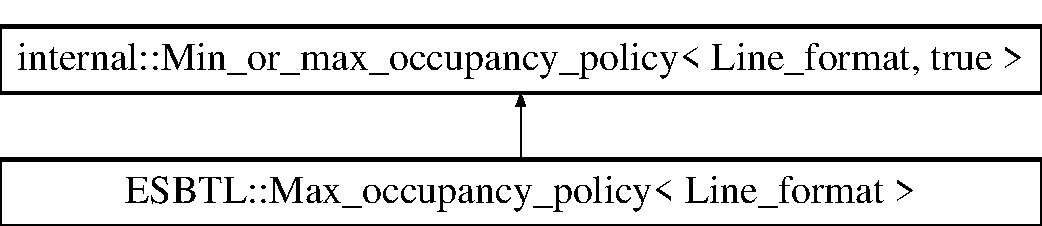
\includegraphics[height=2.000000cm]{classESBTL_1_1Max__occupancy__policy}
\end{center}
\end{figure}


\subsection{Detailed Description}
\subsubsection*{template$<$class Line\+\_\+format$>$\newline
class E\+S\+B\+T\+L\+::\+Max\+\_\+occupancy\+\_\+policy$<$ Line\+\_\+format $>$}

This object provides an occupancy policy. An atom with an occupancy != 1 and with no alternate location is kept if its occupancy value corresponds to the highest found while reading a molecular structure. Note that if a line have been discarded by the selector, then its occupancy value have not been taken into account for computing the maximum. In case of ambiguous maximum (0.\+5), the program will crash with an error message. 
\begin{DoxyTemplParams}{Template Parameters}
{\em Line\+\_\+format} & is a helper class to read molecular data files such as \hyperlink{classESBTL_1_1PDB_1_1Line__format}{E\+S\+B\+T\+L\+::\+P\+D\+B\+::\+Line\+\_\+format}. \\
\hline
\end{DoxyTemplParams}


The documentation for this class was generated from the following file\+:\begin{DoxyCompactItemize}
\item 
\hyperlink{occupancy__handlers_8h}{occupancy\+\_\+handlers.\+h}\end{DoxyCompactItemize}

\hypertarget{classESBTL_1_1Min__occupancy__policy}{}\section{E\+S\+B\+TL\+:\+:Min\+\_\+occupancy\+\_\+policy$<$ Line\+\_\+format $>$ Class Template Reference}
\label{classESBTL_1_1Min__occupancy__policy}\index{E\+S\+B\+T\+L\+::\+Min\+\_\+occupancy\+\_\+policy$<$ Line\+\_\+format $>$@{E\+S\+B\+T\+L\+::\+Min\+\_\+occupancy\+\_\+policy$<$ Line\+\_\+format $>$}}


{\ttfamily \#include $<$occupancy\+\_\+handlers.\+h$>$}

Inheritance diagram for E\+S\+B\+TL\+:\+:Min\+\_\+occupancy\+\_\+policy$<$ Line\+\_\+format $>$\+:\begin{figure}[H]
\begin{center}
\leavevmode
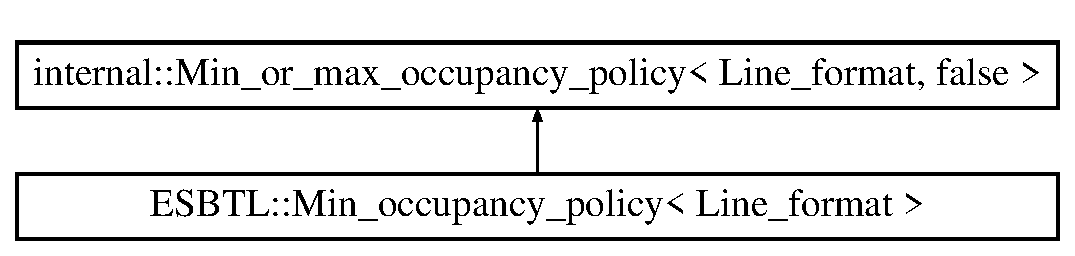
\includegraphics[height=2.000000cm]{classESBTL_1_1Min__occupancy__policy}
\end{center}
\end{figure}


\subsection{Detailed Description}
\subsubsection*{template$<$class Line\+\_\+format$>$\newline
class E\+S\+B\+T\+L\+::\+Min\+\_\+occupancy\+\_\+policy$<$ Line\+\_\+format $>$}

This object provides an occupancy policy. An atom with an occupancy != 1 and with no alternate location is kept if its occupancy value corresponds to the lowest found while reading a molecular structure. Note that if a line have been discarded by the selector, then its occupancy value have not been taken into account for computing the minimum. In case of ambiguous minimum (0.\+5), the program will crash with an error message. 
\begin{DoxyTemplParams}{Template Parameters}
{\em Line\+\_\+format} & is a helper class to read molecular data files such as \hyperlink{classESBTL_1_1PDB_1_1Line__format}{E\+S\+B\+T\+L\+::\+P\+D\+B\+::\+Line\+\_\+format}. \\
\hline
\end{DoxyTemplParams}


The documentation for this class was generated from the following file\+:\begin{DoxyCompactItemize}
\item 
\hyperlink{occupancy__handlers_8h}{occupancy\+\_\+handlers.\+h}\end{DoxyCompactItemize}

\hypertarget{structESBTL_1_1Default__system__items_1_1Model__wrapper}{}\section{E\+S\+B\+TL\+:\+:Default\+\_\+system\+\_\+items\+:\+:Model\+\_\+wrapper$<$ System, Point $>$ Struct Template Reference}
\label{structESBTL_1_1Default__system__items_1_1Model__wrapper}\index{E\+S\+B\+T\+L\+::\+Default\+\_\+system\+\_\+items\+::\+Model\+\_\+wrapper$<$ System, Point $>$@{E\+S\+B\+T\+L\+::\+Default\+\_\+system\+\_\+items\+::\+Model\+\_\+wrapper$<$ System, Point $>$}}


{\ttfamily \#include $<$molecular\+\_\+system.\+h$>$}

\subsection*{Public Types}
\begin{DoxyCompactItemize}
\item 
typedef \hyperlink{classESBTL_1_1Molecular__model}{Molecular\+\_\+model}$<$ System $>$ \hyperlink{structESBTL_1_1Default__system__items_1_1Model__wrapper_a00b684fbb88970776e2fb2495a3ee64c}{Type}
\end{DoxyCompactItemize}


\subsection{Member Typedef Documentation}
\mbox{\Hypertarget{structESBTL_1_1Default__system__items_1_1Model__wrapper_a00b684fbb88970776e2fb2495a3ee64c}\label{structESBTL_1_1Default__system__items_1_1Model__wrapper_a00b684fbb88970776e2fb2495a3ee64c}} 
\index{E\+S\+B\+T\+L\+::\+Default\+\_\+system\+\_\+items\+::\+Model\+\_\+wrapper@{E\+S\+B\+T\+L\+::\+Default\+\_\+system\+\_\+items\+::\+Model\+\_\+wrapper}!Type@{Type}}
\index{Type@{Type}!E\+S\+B\+T\+L\+::\+Default\+\_\+system\+\_\+items\+::\+Model\+\_\+wrapper@{E\+S\+B\+T\+L\+::\+Default\+\_\+system\+\_\+items\+::\+Model\+\_\+wrapper}}
\subsubsection{\texorpdfstring{Type}{Type}}
{\footnotesize\ttfamily template$<$class System , class Point $>$ \\
typedef \hyperlink{classESBTL_1_1Molecular__model}{Molecular\+\_\+model}$<$System$>$ \hyperlink{structESBTL_1_1Default__system__items_1_1Model__wrapper}{E\+S\+B\+T\+L\+::\+Default\+\_\+system\+\_\+items\+::\+Model\+\_\+wrapper}$<$ System, Point $>$\+::\hyperlink{structESBTL_1_1Default__system__items_1_1Model__wrapper_a00b684fbb88970776e2fb2495a3ee64c}{Type}}



The documentation for this struct was generated from the following file\+:\begin{DoxyCompactItemize}
\item 
\hyperlink{molecular__system_8h}{molecular\+\_\+system.\+h}\end{DoxyCompactItemize}

\hypertarget{structESBTL_1_1System__items__with__coarse__grain_1_1Model__wrapper}{}\section{E\+S\+B\+TL\+:\+:System\+\_\+items\+\_\+with\+\_\+coarse\+\_\+grain\+:\+:Model\+\_\+wrapper$<$ System, Point\+\_\+3 $>$ Struct Template Reference}
\label{structESBTL_1_1System__items__with__coarse__grain_1_1Model__wrapper}\index{E\+S\+B\+T\+L\+::\+System\+\_\+items\+\_\+with\+\_\+coarse\+\_\+grain\+::\+Model\+\_\+wrapper$<$ System, Point\+\_\+3 $>$@{E\+S\+B\+T\+L\+::\+System\+\_\+items\+\_\+with\+\_\+coarse\+\_\+grain\+::\+Model\+\_\+wrapper$<$ System, Point\+\_\+3 $>$}}


{\ttfamily \#include $<$coarse\+\_\+grain.\+h$>$}

\subsection*{Public Types}
\begin{DoxyCompactItemize}
\item 
typedef \hyperlink{classESBTL_1_1Molecular__model}{Molecular\+\_\+model}$<$ System $>$ \hyperlink{structESBTL_1_1System__items__with__coarse__grain_1_1Model__wrapper_a051912c005f26be4419a9352b3362044}{Type}
\end{DoxyCompactItemize}


\subsection{Member Typedef Documentation}
\mbox{\Hypertarget{structESBTL_1_1System__items__with__coarse__grain_1_1Model__wrapper_a051912c005f26be4419a9352b3362044}\label{structESBTL_1_1System__items__with__coarse__grain_1_1Model__wrapper_a051912c005f26be4419a9352b3362044}} 
\index{E\+S\+B\+T\+L\+::\+System\+\_\+items\+\_\+with\+\_\+coarse\+\_\+grain\+::\+Model\+\_\+wrapper@{E\+S\+B\+T\+L\+::\+System\+\_\+items\+\_\+with\+\_\+coarse\+\_\+grain\+::\+Model\+\_\+wrapper}!Type@{Type}}
\index{Type@{Type}!E\+S\+B\+T\+L\+::\+System\+\_\+items\+\_\+with\+\_\+coarse\+\_\+grain\+::\+Model\+\_\+wrapper@{E\+S\+B\+T\+L\+::\+System\+\_\+items\+\_\+with\+\_\+coarse\+\_\+grain\+::\+Model\+\_\+wrapper}}
\subsubsection{\texorpdfstring{Type}{Type}}
{\footnotesize\ttfamily template$<$class System , class Point\+\_\+3 $>$ \\
typedef \hyperlink{classESBTL_1_1Molecular__model}{Molecular\+\_\+model}$<$System$>$ \hyperlink{structESBTL_1_1System__items__with__coarse__grain_1_1Model__wrapper}{E\+S\+B\+T\+L\+::\+System\+\_\+items\+\_\+with\+\_\+coarse\+\_\+grain\+::\+Model\+\_\+wrapper}$<$ System, \hyperlink{classESBTL_1_1Point__3}{Point\+\_\+3} $>$\+::\hyperlink{structESBTL_1_1System__items__with__coarse__grain_1_1Model__wrapper_a051912c005f26be4419a9352b3362044}{Type}}



The documentation for this struct was generated from the following file\+:\begin{DoxyCompactItemize}
\item 
\hyperlink{coarse__grain_8h}{coarse\+\_\+grain.\+h}\end{DoxyCompactItemize}

\hypertarget{classESBTL_1_1Molecular__atom}{}\section{E\+S\+B\+TL\+:\+:Molecular\+\_\+atom$<$ System\+\_\+, Point $>$ Class Template Reference}
\label{classESBTL_1_1Molecular__atom}\index{E\+S\+B\+T\+L\+::\+Molecular\+\_\+atom$<$ System\+\_\+, Point $>$@{E\+S\+B\+T\+L\+::\+Molecular\+\_\+atom$<$ System\+\_\+, Point $>$}}


{\ttfamily \#include $<$molecular\+\_\+system.\+h$>$}

Inheritance diagram for E\+S\+B\+TL\+:\+:Molecular\+\_\+atom$<$ System\+\_\+, Point $>$\+:\begin{figure}[H]
\begin{center}
\leavevmode
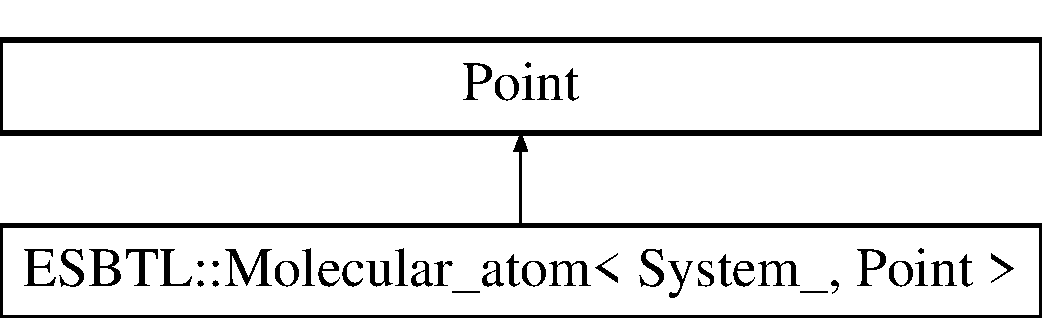
\includegraphics[height=2.000000cm]{classESBTL_1_1Molecular__atom}
\end{center}
\end{figure}
\subsection*{Public Types}
\begin{DoxyCompactItemize}
\item 
typedef System\+\_\+ \hyperlink{classESBTL_1_1Molecular__atom_a58dc16da7581815290469a77906ff8f2}{System}
\item 
typedef Point \hyperlink{classESBTL_1_1Molecular__atom_a7803bad1194caa2c54a055a1e8f0c3fb}{Point\+\_\+3}
\item 
typedef System\+::\+Residue \hyperlink{classESBTL_1_1Molecular__atom_a24e68b497c2f43b77ca43be36af7bcd1}{Residue}
\end{DoxyCompactItemize}
\subsection*{Public Member Functions}
\begin{DoxyCompactItemize}
\item 
{\footnotesize template$<$class Line\+\_\+format , class Residue\+\_\+type $>$ }\\\hyperlink{classESBTL_1_1Molecular__atom_ac32221d9e98536591fae017386cd4d82}{Molecular\+\_\+atom} (const Line\+\_\+format \&line\+\_\+format, const std\+::string \&line, const Residue\+\_\+type \&res)
\item 
\hyperlink{classESBTL_1_1Molecular__atom_a628dcff0a6307d4e49bb8a295ad2bd9f}{Molecular\+\_\+atom} ()
\item 
\hyperlink{classESBTL_1_1Molecular__atom_a5ce88fe393e6b78ac28de314a458461b}{Molecular\+\_\+atom} (double x, double y, double z)
\item 
int \hyperlink{classESBTL_1_1Molecular__atom_aa82969b5f5bb9bd0f59f4ad6548ea756}{system\+\_\+index} () const
\item 
char \hyperlink{classESBTL_1_1Molecular__atom_a2a3e6ea3f4491a81b4b4f77ae28e8f09}{chain\+\_\+identifier} () const
\item 
const \hyperlink{classESBTL_1_1Molecular__atom_a24e68b497c2f43b77ca43be36af7bcd1}{Residue} \& \hyperlink{classESBTL_1_1Molecular__atom_a96a14b402625e528a38410c5b483b8ac}{residue} () const
\item 
const std\+::string \& \hyperlink{classESBTL_1_1Molecular__atom_a61d6ee7dda9e312112eb433cf96ffa2e}{residue\+\_\+name} () const
\item 
int \hyperlink{classESBTL_1_1Molecular__atom_a0ac28cedb09615d293a6b3ed026f52d7}{residue\+\_\+sequence\+\_\+number} () const
\item 
char \hyperlink{classESBTL_1_1Molecular__atom_ab3624555c42198359e9f0e8e5914ba3e}{insertion\+\_\+code} () const
\end{DoxyCompactItemize}


\subsection{Detailed Description}
\subsubsection*{template$<$class System\+\_\+, class Point$>$\newline
class E\+S\+B\+T\+L\+::\+Molecular\+\_\+atom$<$ System\+\_\+, Point $>$}

A class representing an atom. 
\begin{DoxyTemplParams}{Template Parameters}
{\em System\+\_\+} & is a system (like \hyperlink{classESBTL_1_1Molecular__system}{E\+S\+B\+T\+L\+::\+Molecular\+\_\+system} for example). \\
\hline
{\em Point} & is a point type with coordinates const access methods x(), y() and z(). \\
\hline
\end{DoxyTemplParams}


\subsection{Member Typedef Documentation}
\mbox{\Hypertarget{classESBTL_1_1Molecular__atom_a7803bad1194caa2c54a055a1e8f0c3fb}\label{classESBTL_1_1Molecular__atom_a7803bad1194caa2c54a055a1e8f0c3fb}} 
\index{E\+S\+B\+T\+L\+::\+Molecular\+\_\+atom@{E\+S\+B\+T\+L\+::\+Molecular\+\_\+atom}!Point\+\_\+3@{Point\+\_\+3}}
\index{Point\+\_\+3@{Point\+\_\+3}!E\+S\+B\+T\+L\+::\+Molecular\+\_\+atom@{E\+S\+B\+T\+L\+::\+Molecular\+\_\+atom}}
\subsubsection{\texorpdfstring{Point\+\_\+3}{Point\_3}}
{\footnotesize\ttfamily template$<$class System\+\_\+, class Point$>$ \\
typedef Point \hyperlink{classESBTL_1_1Molecular__atom}{E\+S\+B\+T\+L\+::\+Molecular\+\_\+atom}$<$ System\+\_\+, Point $>$\+::\hyperlink{classESBTL_1_1Molecular__atom_a7803bad1194caa2c54a055a1e8f0c3fb}{Point\+\_\+3}}

\mbox{\Hypertarget{classESBTL_1_1Molecular__atom_a24e68b497c2f43b77ca43be36af7bcd1}\label{classESBTL_1_1Molecular__atom_a24e68b497c2f43b77ca43be36af7bcd1}} 
\index{E\+S\+B\+T\+L\+::\+Molecular\+\_\+atom@{E\+S\+B\+T\+L\+::\+Molecular\+\_\+atom}!Residue@{Residue}}
\index{Residue@{Residue}!E\+S\+B\+T\+L\+::\+Molecular\+\_\+atom@{E\+S\+B\+T\+L\+::\+Molecular\+\_\+atom}}
\subsubsection{\texorpdfstring{Residue}{Residue}}
{\footnotesize\ttfamily template$<$class System\+\_\+, class Point$>$ \\
typedef System\+::\+Residue \hyperlink{classESBTL_1_1Molecular__atom}{E\+S\+B\+T\+L\+::\+Molecular\+\_\+atom}$<$ System\+\_\+, Point $>$\+::\hyperlink{classESBTL_1_1Molecular__atom_a24e68b497c2f43b77ca43be36af7bcd1}{Residue}}

\mbox{\Hypertarget{classESBTL_1_1Molecular__atom_a58dc16da7581815290469a77906ff8f2}\label{classESBTL_1_1Molecular__atom_a58dc16da7581815290469a77906ff8f2}} 
\index{E\+S\+B\+T\+L\+::\+Molecular\+\_\+atom@{E\+S\+B\+T\+L\+::\+Molecular\+\_\+atom}!System@{System}}
\index{System@{System}!E\+S\+B\+T\+L\+::\+Molecular\+\_\+atom@{E\+S\+B\+T\+L\+::\+Molecular\+\_\+atom}}
\subsubsection{\texorpdfstring{System}{System}}
{\footnotesize\ttfamily template$<$class System\+\_\+, class Point$>$ \\
typedef System\+\_\+ \hyperlink{classESBTL_1_1Molecular__atom}{E\+S\+B\+T\+L\+::\+Molecular\+\_\+atom}$<$ System\+\_\+, Point $>$\+::\hyperlink{classESBTL_1_1Molecular__atom_a58dc16da7581815290469a77906ff8f2}{System}}



\subsection{Constructor \& Destructor Documentation}
\mbox{\Hypertarget{classESBTL_1_1Molecular__atom_ac32221d9e98536591fae017386cd4d82}\label{classESBTL_1_1Molecular__atom_ac32221d9e98536591fae017386cd4d82}} 
\index{E\+S\+B\+T\+L\+::\+Molecular\+\_\+atom@{E\+S\+B\+T\+L\+::\+Molecular\+\_\+atom}!Molecular\+\_\+atom@{Molecular\+\_\+atom}}
\index{Molecular\+\_\+atom@{Molecular\+\_\+atom}!E\+S\+B\+T\+L\+::\+Molecular\+\_\+atom@{E\+S\+B\+T\+L\+::\+Molecular\+\_\+atom}}
\subsubsection{\texorpdfstring{Molecular\+\_\+atom()}{Molecular\_atom()}\hspace{0.1cm}{\footnotesize\ttfamily [1/3]}}
{\footnotesize\ttfamily template$<$class System\+\_\+, class Point$>$ \\
template$<$class Line\+\_\+format , class Residue\+\_\+type $>$ \\
\hyperlink{classESBTL_1_1Molecular__atom}{E\+S\+B\+T\+L\+::\+Molecular\+\_\+atom}$<$ System\+\_\+, Point $>$\+::\hyperlink{classESBTL_1_1Molecular__atom}{Molecular\+\_\+atom} (\begin{DoxyParamCaption}\item[{const Line\+\_\+format \&}]{line\+\_\+format,  }\item[{const std\+::string \&}]{line,  }\item[{const Residue\+\_\+type \&}]{res }\end{DoxyParamCaption})\hspace{0.3cm}{\ttfamily [inline]}}

\mbox{\Hypertarget{classESBTL_1_1Molecular__atom_a628dcff0a6307d4e49bb8a295ad2bd9f}\label{classESBTL_1_1Molecular__atom_a628dcff0a6307d4e49bb8a295ad2bd9f}} 
\index{E\+S\+B\+T\+L\+::\+Molecular\+\_\+atom@{E\+S\+B\+T\+L\+::\+Molecular\+\_\+atom}!Molecular\+\_\+atom@{Molecular\+\_\+atom}}
\index{Molecular\+\_\+atom@{Molecular\+\_\+atom}!E\+S\+B\+T\+L\+::\+Molecular\+\_\+atom@{E\+S\+B\+T\+L\+::\+Molecular\+\_\+atom}}
\subsubsection{\texorpdfstring{Molecular\+\_\+atom()}{Molecular\_atom()}\hspace{0.1cm}{\footnotesize\ttfamily [2/3]}}
{\footnotesize\ttfamily template$<$class System\+\_\+, class Point$>$ \\
\hyperlink{classESBTL_1_1Molecular__atom}{E\+S\+B\+T\+L\+::\+Molecular\+\_\+atom}$<$ System\+\_\+, Point $>$\+::\hyperlink{classESBTL_1_1Molecular__atom}{Molecular\+\_\+atom} (\begin{DoxyParamCaption}{ }\end{DoxyParamCaption})\hspace{0.3cm}{\ttfamily [inline]}}

\mbox{\Hypertarget{classESBTL_1_1Molecular__atom_a5ce88fe393e6b78ac28de314a458461b}\label{classESBTL_1_1Molecular__atom_a5ce88fe393e6b78ac28de314a458461b}} 
\index{E\+S\+B\+T\+L\+::\+Molecular\+\_\+atom@{E\+S\+B\+T\+L\+::\+Molecular\+\_\+atom}!Molecular\+\_\+atom@{Molecular\+\_\+atom}}
\index{Molecular\+\_\+atom@{Molecular\+\_\+atom}!E\+S\+B\+T\+L\+::\+Molecular\+\_\+atom@{E\+S\+B\+T\+L\+::\+Molecular\+\_\+atom}}
\subsubsection{\texorpdfstring{Molecular\+\_\+atom()}{Molecular\_atom()}\hspace{0.1cm}{\footnotesize\ttfamily [3/3]}}
{\footnotesize\ttfamily template$<$class System\+\_\+, class Point$>$ \\
\hyperlink{classESBTL_1_1Molecular__atom}{E\+S\+B\+T\+L\+::\+Molecular\+\_\+atom}$<$ System\+\_\+, Point $>$\+::\hyperlink{classESBTL_1_1Molecular__atom}{Molecular\+\_\+atom} (\begin{DoxyParamCaption}\item[{double}]{x,  }\item[{double}]{y,  }\item[{double}]{z }\end{DoxyParamCaption})\hspace{0.3cm}{\ttfamily [inline]}}



\subsection{Member Function Documentation}
\mbox{\Hypertarget{classESBTL_1_1Molecular__atom_a2a3e6ea3f4491a81b4b4f77ae28e8f09}\label{classESBTL_1_1Molecular__atom_a2a3e6ea3f4491a81b4b4f77ae28e8f09}} 
\index{E\+S\+B\+T\+L\+::\+Molecular\+\_\+atom@{E\+S\+B\+T\+L\+::\+Molecular\+\_\+atom}!chain\+\_\+identifier@{chain\+\_\+identifier}}
\index{chain\+\_\+identifier@{chain\+\_\+identifier}!E\+S\+B\+T\+L\+::\+Molecular\+\_\+atom@{E\+S\+B\+T\+L\+::\+Molecular\+\_\+atom}}
\subsubsection{\texorpdfstring{chain\+\_\+identifier()}{chain\_identifier()}}
{\footnotesize\ttfamily template$<$class System\+\_\+, class Point$>$ \\
char \hyperlink{classESBTL_1_1Molecular__atom}{E\+S\+B\+T\+L\+::\+Molecular\+\_\+atom}$<$ System\+\_\+, Point $>$\+::chain\+\_\+identifier (\begin{DoxyParamCaption}{ }\end{DoxyParamCaption}) const\hspace{0.3cm}{\ttfamily [inline]}}

\mbox{\Hypertarget{classESBTL_1_1Molecular__atom_ab3624555c42198359e9f0e8e5914ba3e}\label{classESBTL_1_1Molecular__atom_ab3624555c42198359e9f0e8e5914ba3e}} 
\index{E\+S\+B\+T\+L\+::\+Molecular\+\_\+atom@{E\+S\+B\+T\+L\+::\+Molecular\+\_\+atom}!insertion\+\_\+code@{insertion\+\_\+code}}
\index{insertion\+\_\+code@{insertion\+\_\+code}!E\+S\+B\+T\+L\+::\+Molecular\+\_\+atom@{E\+S\+B\+T\+L\+::\+Molecular\+\_\+atom}}
\subsubsection{\texorpdfstring{insertion\+\_\+code()}{insertion\_code()}}
{\footnotesize\ttfamily template$<$class System\+\_\+, class Point$>$ \\
char \hyperlink{classESBTL_1_1Molecular__atom}{E\+S\+B\+T\+L\+::\+Molecular\+\_\+atom}$<$ System\+\_\+, Point $>$\+::insertion\+\_\+code (\begin{DoxyParamCaption}{ }\end{DoxyParamCaption}) const\hspace{0.3cm}{\ttfamily [inline]}}

\mbox{\Hypertarget{classESBTL_1_1Molecular__atom_a96a14b402625e528a38410c5b483b8ac}\label{classESBTL_1_1Molecular__atom_a96a14b402625e528a38410c5b483b8ac}} 
\index{E\+S\+B\+T\+L\+::\+Molecular\+\_\+atom@{E\+S\+B\+T\+L\+::\+Molecular\+\_\+atom}!residue@{residue}}
\index{residue@{residue}!E\+S\+B\+T\+L\+::\+Molecular\+\_\+atom@{E\+S\+B\+T\+L\+::\+Molecular\+\_\+atom}}
\subsubsection{\texorpdfstring{residue()}{residue()}}
{\footnotesize\ttfamily template$<$class System\+\_\+, class Point$>$ \\
const \hyperlink{classESBTL_1_1Molecular__atom_a24e68b497c2f43b77ca43be36af7bcd1}{Residue}\& \hyperlink{classESBTL_1_1Molecular__atom}{E\+S\+B\+T\+L\+::\+Molecular\+\_\+atom}$<$ System\+\_\+, Point $>$\+::residue (\begin{DoxyParamCaption}{ }\end{DoxyParamCaption}) const\hspace{0.3cm}{\ttfamily [inline]}}

\mbox{\Hypertarget{classESBTL_1_1Molecular__atom_a61d6ee7dda9e312112eb433cf96ffa2e}\label{classESBTL_1_1Molecular__atom_a61d6ee7dda9e312112eb433cf96ffa2e}} 
\index{E\+S\+B\+T\+L\+::\+Molecular\+\_\+atom@{E\+S\+B\+T\+L\+::\+Molecular\+\_\+atom}!residue\+\_\+name@{residue\+\_\+name}}
\index{residue\+\_\+name@{residue\+\_\+name}!E\+S\+B\+T\+L\+::\+Molecular\+\_\+atom@{E\+S\+B\+T\+L\+::\+Molecular\+\_\+atom}}
\subsubsection{\texorpdfstring{residue\+\_\+name()}{residue\_name()}}
{\footnotesize\ttfamily template$<$class System\+\_\+, class Point$>$ \\
const std\+::string\& \hyperlink{classESBTL_1_1Molecular__atom}{E\+S\+B\+T\+L\+::\+Molecular\+\_\+atom}$<$ System\+\_\+, Point $>$\+::residue\+\_\+name (\begin{DoxyParamCaption}{ }\end{DoxyParamCaption}) const\hspace{0.3cm}{\ttfamily [inline]}}

\mbox{\Hypertarget{classESBTL_1_1Molecular__atom_a0ac28cedb09615d293a6b3ed026f52d7}\label{classESBTL_1_1Molecular__atom_a0ac28cedb09615d293a6b3ed026f52d7}} 
\index{E\+S\+B\+T\+L\+::\+Molecular\+\_\+atom@{E\+S\+B\+T\+L\+::\+Molecular\+\_\+atom}!residue\+\_\+sequence\+\_\+number@{residue\+\_\+sequence\+\_\+number}}
\index{residue\+\_\+sequence\+\_\+number@{residue\+\_\+sequence\+\_\+number}!E\+S\+B\+T\+L\+::\+Molecular\+\_\+atom@{E\+S\+B\+T\+L\+::\+Molecular\+\_\+atom}}
\subsubsection{\texorpdfstring{residue\+\_\+sequence\+\_\+number()}{residue\_sequence\_number()}}
{\footnotesize\ttfamily template$<$class System\+\_\+, class Point$>$ \\
int \hyperlink{classESBTL_1_1Molecular__atom}{E\+S\+B\+T\+L\+::\+Molecular\+\_\+atom}$<$ System\+\_\+, Point $>$\+::residue\+\_\+sequence\+\_\+number (\begin{DoxyParamCaption}{ }\end{DoxyParamCaption}) const\hspace{0.3cm}{\ttfamily [inline]}}

\mbox{\Hypertarget{classESBTL_1_1Molecular__atom_aa82969b5f5bb9bd0f59f4ad6548ea756}\label{classESBTL_1_1Molecular__atom_aa82969b5f5bb9bd0f59f4ad6548ea756}} 
\index{E\+S\+B\+T\+L\+::\+Molecular\+\_\+atom@{E\+S\+B\+T\+L\+::\+Molecular\+\_\+atom}!system\+\_\+index@{system\+\_\+index}}
\index{system\+\_\+index@{system\+\_\+index}!E\+S\+B\+T\+L\+::\+Molecular\+\_\+atom@{E\+S\+B\+T\+L\+::\+Molecular\+\_\+atom}}
\subsubsection{\texorpdfstring{system\+\_\+index()}{system\_index()}}
{\footnotesize\ttfamily template$<$class System\+\_\+, class Point$>$ \\
int \hyperlink{classESBTL_1_1Molecular__atom}{E\+S\+B\+T\+L\+::\+Molecular\+\_\+atom}$<$ System\+\_\+, Point $>$\+::system\+\_\+index (\begin{DoxyParamCaption}{ }\end{DoxyParamCaption}) const\hspace{0.3cm}{\ttfamily [inline]}}



The documentation for this class was generated from the following file\+:\begin{DoxyCompactItemize}
\item 
\hyperlink{molecular__system_8h}{molecular\+\_\+system.\+h}\end{DoxyCompactItemize}

\hypertarget{classESBTL_1_1Molecular__chain}{}\section{E\+S\+B\+TL\+:\+:Molecular\+\_\+chain$<$ System $>$ Class Template Reference}
\label{classESBTL_1_1Molecular__chain}\index{E\+S\+B\+T\+L\+::\+Molecular\+\_\+chain$<$ System $>$@{E\+S\+B\+T\+L\+::\+Molecular\+\_\+chain$<$ System $>$}}


{\ttfamily \#include $<$molecular\+\_\+system.\+h$>$}

\subsection*{Public Types}
\begin{DoxyCompactItemize}
\item 
typedef System\+::\+Residue \hyperlink{classESBTL_1_1Molecular__chain_a59b61e0ecde5fb4c3d1765a37c9cf6cb}{Residue}
\item 
typedef Residue\+::\+Atom \hyperlink{classESBTL_1_1Molecular__chain_a53b9fe27aadbda89ae35802db0493405}{Atom}
\item 
typedef std\+::map$<$ std\+::pair$<$ int, char $>$, \hyperlink{classESBTL_1_1Molecular__chain_a59b61e0ecde5fb4c3d1765a37c9cf6cb}{Residue} $>$ \hyperlink{classESBTL_1_1Molecular__chain_a23f0241e8d12867ed7eb6f1ed862e2ef}{Residue\+\_\+container}
\item 
typedef System\+::\+Model \hyperlink{classESBTL_1_1Molecular__chain_a91de91fd0923cf2e00d947b76851be68}{Model}
\item 
typedef internal\+::\+Residues\+\_\+iterator\+\_\+from\+\_\+chain$<$ \hyperlink{classESBTL_1_1Molecular__chain}{Self}, true $>$ \hyperlink{group__grp__iters_ga4cadd9ac293bcd967a86f97bfc626a7f}{Residues\+\_\+const\+\_\+iterator}
\item 
typedef internal\+::\+Residues\+\_\+iterator\+\_\+from\+\_\+chain$<$ \hyperlink{classESBTL_1_1Molecular__chain}{Self}, false $>$ \hyperlink{group__grp__iters_gaccad04117ad7c730e41bdb9aeab8f116}{Residues\+\_\+iterator}
\item 
typedef internal\+::\+Atoms\+\_\+iterator\+\_\+from\+\_\+chain$<$ \hyperlink{classESBTL_1_1Molecular__chain}{Self}, true $>$ \hyperlink{group__grp__iters_gad872d386b268126c9bb2a2127a6a7254}{Atoms\+\_\+const\+\_\+iterator}
\item 
typedef internal\+::\+Atoms\+\_\+iterator\+\_\+from\+\_\+chain$<$ \hyperlink{classESBTL_1_1Molecular__chain}{Self}, false $>$ \hyperlink{group__grp__iters_gab2ee52ce4f9b656648669214cc44a4ea}{Atoms\+\_\+iterator}
\end{DoxyCompactItemize}
\subsection*{Public Member Functions}
\begin{DoxyCompactItemize}
\item 
{\footnotesize template$<$class Line\+\_\+format $>$ }\\\hyperlink{classESBTL_1_1Molecular__chain_a4652d6763dcfcf123450737ebb6eaf5a}{Molecular\+\_\+chain} (const Line\+\_\+format \&line\+\_\+format, const std\+::string \&line, const \hyperlink{classESBTL_1_1Molecular__chain_a91de91fd0923cf2e00d947b76851be68}{Model} \&mod)
\item 
\hyperlink{classESBTL_1_1Molecular__chain_a6a6ccadbd35d571991d63058f9d2b571}{Molecular\+\_\+chain} (char id, const \hyperlink{classESBTL_1_1Molecular__chain_a91de91fd0923cf2e00d947b76851be68}{Model} \&mod)
\item 
const \hyperlink{classESBTL_1_1Molecular__chain_a91de91fd0923cf2e00d947b76851be68}{Model} \& \hyperlink{classESBTL_1_1Molecular__chain_a6383517afc2e91d6a4b1c6759fb0fe24}{model} () const
\item 
{\footnotesize template$<$class Line\+\_\+format $>$ }\\\hyperlink{classESBTL_1_1Molecular__chain_a59b61e0ecde5fb4c3d1765a37c9cf6cb}{Residue} \& \hyperlink{classESBTL_1_1Molecular__chain_a4b4f28e5fde3c5b42f1bb236f21c6c5d}{get\+\_\+or\+\_\+create\+\_\+residue} (const Line\+\_\+format \&line\+\_\+format, const std\+::string \&line)
\item 
\hyperlink{classESBTL_1_1Molecular__chain_a59b61e0ecde5fb4c3d1765a37c9cf6cb}{Residue} \& \hyperlink{classESBTL_1_1Molecular__chain_aa35aa61329884011dc85906c387df84c}{get\+\_\+or\+\_\+create\+\_\+residue} (const std\+::string \&resname, int ressn, char insc)
\item 
const \hyperlink{classESBTL_1_1Molecular__chain_a59b61e0ecde5fb4c3d1765a37c9cf6cb}{Residue} \& \hyperlink{classESBTL_1_1Molecular__chain_add9e2713daf6374d29fc32bd0dc93ccf}{get\+\_\+residue} (int ressn, char insc=\textquotesingle{} \textquotesingle{})
\item 
const System\+::\+Atom \hyperlink{classESBTL_1_1Molecular__chain_a79ec125306145c87a869a1d966700c75}{get\+\_\+atom} (int ressn, char insc, unsigned atom\+\_\+sn) const
\item 
size\+\_\+t \hyperlink{classESBTL_1_1Molecular__chain_ae2cb5ee5dddeb528c705e293d575e0a1}{number\+\_\+of\+\_\+residues} () const
\item 
size\+\_\+t \hyperlink{classESBTL_1_1Molecular__chain_a1ca00f968e6e4bc79c4392eb86d2d865}{number\+\_\+of\+\_\+atoms} () const
\item 
\hyperlink{group__grp__iters_gaccad04117ad7c730e41bdb9aeab8f116}{Residues\+\_\+iterator} \hyperlink{group__grp__iters_ga5785a87f04fb8ffefaaf46c6f341b05d}{residues\+\_\+begin} ()
\item 
\hyperlink{group__grp__iters_gaccad04117ad7c730e41bdb9aeab8f116}{Residues\+\_\+iterator} \hyperlink{group__grp__iters_gaee7c0abec465c6523f3095f2e2f6a8b8}{residues\+\_\+end} ()
\item 
\hyperlink{group__grp__iters_ga4cadd9ac293bcd967a86f97bfc626a7f}{Residues\+\_\+const\+\_\+iterator} \hyperlink{group__grp__iters_ga7638b8fd914f2fb1895cfd02c79b1e5d}{residues\+\_\+begin} () const
\item 
\hyperlink{group__grp__iters_ga4cadd9ac293bcd967a86f97bfc626a7f}{Residues\+\_\+const\+\_\+iterator} \hyperlink{group__grp__iters_ga074337267e031ed306dfa7048e3bb692}{residues\+\_\+end} () const
\item 
\hyperlink{group__grp__iters_gab2ee52ce4f9b656648669214cc44a4ea}{Atoms\+\_\+iterator} \hyperlink{group__grp__iters_gafd79068d582c1a588cf3843fcac1d55d}{atoms\+\_\+begin} ()
\item 
\hyperlink{group__grp__iters_gab2ee52ce4f9b656648669214cc44a4ea}{Atoms\+\_\+iterator} \hyperlink{group__grp__iters_gaaacb84783e8dd81f5013c85165b3707b}{atoms\+\_\+end} ()
\item 
\hyperlink{group__grp__iters_gad872d386b268126c9bb2a2127a6a7254}{Atoms\+\_\+const\+\_\+iterator} \hyperlink{group__grp__iters_gac6ba7621f15096a4633db8b112fd05fe}{atoms\+\_\+begin} () const
\item 
\hyperlink{group__grp__iters_gad872d386b268126c9bb2a2127a6a7254}{Atoms\+\_\+const\+\_\+iterator} \hyperlink{group__grp__iters_ga925ea88c3cb1be749a9256b9ea77bc79}{atoms\+\_\+end} () const
\end{DoxyCompactItemize}
\subsection*{Static Public Member Functions}
\begin{DoxyCompactItemize}
\item 
static const \hyperlink{classESBTL_1_1Molecular__chain_a59b61e0ecde5fb4c3d1765a37c9cf6cb}{Residue} \& \hyperlink{classESBTL_1_1Molecular__chain_a8b33c52b188ce7704ffd12bdbdf13d68}{dereference} (typename Residue\+\_\+container\+::const\+\_\+iterator it)
\item 
static \hyperlink{classESBTL_1_1Molecular__chain_a59b61e0ecde5fb4c3d1765a37c9cf6cb}{Residue} \& \hyperlink{classESBTL_1_1Molecular__chain_a82c1f1ae170646c483eba1cbaae17419}{dereference} (typename Residue\+\_\+container\+::iterator it)
\end{DoxyCompactItemize}


\subsection{Detailed Description}
\subsubsection*{template$<$class System$>$\newline
class E\+S\+B\+T\+L\+::\+Molecular\+\_\+chain$<$ System $>$}

A class representing a chain. 
\begin{DoxyTemplParams}{Template Parameters}
{\em System} & is a system (like \hyperlink{classESBTL_1_1Molecular__system}{E\+S\+B\+T\+L\+::\+Molecular\+\_\+system} for example). \\
\hline
\end{DoxyTemplParams}


\subsection{Member Typedef Documentation}
\mbox{\Hypertarget{classESBTL_1_1Molecular__chain_a53b9fe27aadbda89ae35802db0493405}\label{classESBTL_1_1Molecular__chain_a53b9fe27aadbda89ae35802db0493405}} 
\index{E\+S\+B\+T\+L\+::\+Molecular\+\_\+chain@{E\+S\+B\+T\+L\+::\+Molecular\+\_\+chain}!Atom@{Atom}}
\index{Atom@{Atom}!E\+S\+B\+T\+L\+::\+Molecular\+\_\+chain@{E\+S\+B\+T\+L\+::\+Molecular\+\_\+chain}}
\subsubsection{\texorpdfstring{Atom}{Atom}}
{\footnotesize\ttfamily template$<$class System$>$ \\
typedef Residue\+::\+Atom \hyperlink{classESBTL_1_1Molecular__chain}{E\+S\+B\+T\+L\+::\+Molecular\+\_\+chain}$<$ System $>$\+::\hyperlink{classESBTL_1_1Molecular__chain_a53b9fe27aadbda89ae35802db0493405}{Atom}}

\mbox{\Hypertarget{classESBTL_1_1Molecular__chain_a91de91fd0923cf2e00d947b76851be68}\label{classESBTL_1_1Molecular__chain_a91de91fd0923cf2e00d947b76851be68}} 
\index{E\+S\+B\+T\+L\+::\+Molecular\+\_\+chain@{E\+S\+B\+T\+L\+::\+Molecular\+\_\+chain}!Model@{Model}}
\index{Model@{Model}!E\+S\+B\+T\+L\+::\+Molecular\+\_\+chain@{E\+S\+B\+T\+L\+::\+Molecular\+\_\+chain}}
\subsubsection{\texorpdfstring{Model}{Model}}
{\footnotesize\ttfamily template$<$class System$>$ \\
typedef System\+::\+Model \hyperlink{classESBTL_1_1Molecular__chain}{E\+S\+B\+T\+L\+::\+Molecular\+\_\+chain}$<$ System $>$\+::\hyperlink{classESBTL_1_1Molecular__chain_a91de91fd0923cf2e00d947b76851be68}{Model}}

\mbox{\Hypertarget{classESBTL_1_1Molecular__chain_a59b61e0ecde5fb4c3d1765a37c9cf6cb}\label{classESBTL_1_1Molecular__chain_a59b61e0ecde5fb4c3d1765a37c9cf6cb}} 
\index{E\+S\+B\+T\+L\+::\+Molecular\+\_\+chain@{E\+S\+B\+T\+L\+::\+Molecular\+\_\+chain}!Residue@{Residue}}
\index{Residue@{Residue}!E\+S\+B\+T\+L\+::\+Molecular\+\_\+chain@{E\+S\+B\+T\+L\+::\+Molecular\+\_\+chain}}
\subsubsection{\texorpdfstring{Residue}{Residue}}
{\footnotesize\ttfamily template$<$class System$>$ \\
typedef System\+::\+Residue \hyperlink{classESBTL_1_1Molecular__chain}{E\+S\+B\+T\+L\+::\+Molecular\+\_\+chain}$<$ System $>$\+::\hyperlink{classESBTL_1_1Molecular__chain_a59b61e0ecde5fb4c3d1765a37c9cf6cb}{Residue}}

\mbox{\Hypertarget{classESBTL_1_1Molecular__chain_a23f0241e8d12867ed7eb6f1ed862e2ef}\label{classESBTL_1_1Molecular__chain_a23f0241e8d12867ed7eb6f1ed862e2ef}} 
\index{E\+S\+B\+T\+L\+::\+Molecular\+\_\+chain@{E\+S\+B\+T\+L\+::\+Molecular\+\_\+chain}!Residue\+\_\+container@{Residue\+\_\+container}}
\index{Residue\+\_\+container@{Residue\+\_\+container}!E\+S\+B\+T\+L\+::\+Molecular\+\_\+chain@{E\+S\+B\+T\+L\+::\+Molecular\+\_\+chain}}
\subsubsection{\texorpdfstring{Residue\+\_\+container}{Residue\_container}}
{\footnotesize\ttfamily template$<$class System$>$ \\
typedef std\+::map$<$std\+::pair$<$int,char$>$,\hyperlink{classESBTL_1_1Molecular__chain_a59b61e0ecde5fb4c3d1765a37c9cf6cb}{Residue}$>$ \hyperlink{classESBTL_1_1Molecular__chain}{E\+S\+B\+T\+L\+::\+Molecular\+\_\+chain}$<$ System $>$\+::\hyperlink{classESBTL_1_1Molecular__chain_a23f0241e8d12867ed7eb6f1ed862e2ef}{Residue\+\_\+container}}



\subsection{Constructor \& Destructor Documentation}
\mbox{\Hypertarget{classESBTL_1_1Molecular__chain_a4652d6763dcfcf123450737ebb6eaf5a}\label{classESBTL_1_1Molecular__chain_a4652d6763dcfcf123450737ebb6eaf5a}} 
\index{E\+S\+B\+T\+L\+::\+Molecular\+\_\+chain@{E\+S\+B\+T\+L\+::\+Molecular\+\_\+chain}!Molecular\+\_\+chain@{Molecular\+\_\+chain}}
\index{Molecular\+\_\+chain@{Molecular\+\_\+chain}!E\+S\+B\+T\+L\+::\+Molecular\+\_\+chain@{E\+S\+B\+T\+L\+::\+Molecular\+\_\+chain}}
\subsubsection{\texorpdfstring{Molecular\+\_\+chain()}{Molecular\_chain()}\hspace{0.1cm}{\footnotesize\ttfamily [1/2]}}
{\footnotesize\ttfamily template$<$class System$>$ \\
template$<$class Line\+\_\+format $>$ \\
\hyperlink{classESBTL_1_1Molecular__chain}{E\+S\+B\+T\+L\+::\+Molecular\+\_\+chain}$<$ System $>$\+::\hyperlink{classESBTL_1_1Molecular__chain}{Molecular\+\_\+chain} (\begin{DoxyParamCaption}\item[{const Line\+\_\+format \&}]{line\+\_\+format,  }\item[{const std\+::string \&}]{line,  }\item[{const \hyperlink{classESBTL_1_1Molecular__chain_a91de91fd0923cf2e00d947b76851be68}{Model} \&}]{mod }\end{DoxyParamCaption})\hspace{0.3cm}{\ttfamily [inline]}}

\mbox{\Hypertarget{classESBTL_1_1Molecular__chain_a6a6ccadbd35d571991d63058f9d2b571}\label{classESBTL_1_1Molecular__chain_a6a6ccadbd35d571991d63058f9d2b571}} 
\index{E\+S\+B\+T\+L\+::\+Molecular\+\_\+chain@{E\+S\+B\+T\+L\+::\+Molecular\+\_\+chain}!Molecular\+\_\+chain@{Molecular\+\_\+chain}}
\index{Molecular\+\_\+chain@{Molecular\+\_\+chain}!E\+S\+B\+T\+L\+::\+Molecular\+\_\+chain@{E\+S\+B\+T\+L\+::\+Molecular\+\_\+chain}}
\subsubsection{\texorpdfstring{Molecular\+\_\+chain()}{Molecular\_chain()}\hspace{0.1cm}{\footnotesize\ttfamily [2/2]}}
{\footnotesize\ttfamily template$<$class System$>$ \\
\hyperlink{classESBTL_1_1Molecular__chain}{E\+S\+B\+T\+L\+::\+Molecular\+\_\+chain}$<$ System $>$\+::\hyperlink{classESBTL_1_1Molecular__chain}{Molecular\+\_\+chain} (\begin{DoxyParamCaption}\item[{char}]{id,  }\item[{const \hyperlink{classESBTL_1_1Molecular__chain_a91de91fd0923cf2e00d947b76851be68}{Model} \&}]{mod }\end{DoxyParamCaption})\hspace{0.3cm}{\ttfamily [inline]}}



\subsection{Member Function Documentation}
\mbox{\Hypertarget{classESBTL_1_1Molecular__chain_a8b33c52b188ce7704ffd12bdbdf13d68}\label{classESBTL_1_1Molecular__chain_a8b33c52b188ce7704ffd12bdbdf13d68}} 
\index{E\+S\+B\+T\+L\+::\+Molecular\+\_\+chain@{E\+S\+B\+T\+L\+::\+Molecular\+\_\+chain}!dereference@{dereference}}
\index{dereference@{dereference}!E\+S\+B\+T\+L\+::\+Molecular\+\_\+chain@{E\+S\+B\+T\+L\+::\+Molecular\+\_\+chain}}
\subsubsection{\texorpdfstring{dereference()}{dereference()}\hspace{0.1cm}{\footnotesize\ttfamily [1/2]}}
{\footnotesize\ttfamily template$<$class System$>$ \\
static const \hyperlink{classESBTL_1_1Molecular__chain_a59b61e0ecde5fb4c3d1765a37c9cf6cb}{Residue}\& \hyperlink{classESBTL_1_1Molecular__chain}{E\+S\+B\+T\+L\+::\+Molecular\+\_\+chain}$<$ System $>$\+::dereference (\begin{DoxyParamCaption}\item[{typename Residue\+\_\+container\+::const\+\_\+iterator}]{it }\end{DoxyParamCaption})\hspace{0.3cm}{\ttfamily [inline]}, {\ttfamily [static]}}

\mbox{\Hypertarget{classESBTL_1_1Molecular__chain_a82c1f1ae170646c483eba1cbaae17419}\label{classESBTL_1_1Molecular__chain_a82c1f1ae170646c483eba1cbaae17419}} 
\index{E\+S\+B\+T\+L\+::\+Molecular\+\_\+chain@{E\+S\+B\+T\+L\+::\+Molecular\+\_\+chain}!dereference@{dereference}}
\index{dereference@{dereference}!E\+S\+B\+T\+L\+::\+Molecular\+\_\+chain@{E\+S\+B\+T\+L\+::\+Molecular\+\_\+chain}}
\subsubsection{\texorpdfstring{dereference()}{dereference()}\hspace{0.1cm}{\footnotesize\ttfamily [2/2]}}
{\footnotesize\ttfamily template$<$class System$>$ \\
static \hyperlink{classESBTL_1_1Molecular__chain_a59b61e0ecde5fb4c3d1765a37c9cf6cb}{Residue}\& \hyperlink{classESBTL_1_1Molecular__chain}{E\+S\+B\+T\+L\+::\+Molecular\+\_\+chain}$<$ System $>$\+::dereference (\begin{DoxyParamCaption}\item[{typename Residue\+\_\+container\+::iterator}]{it }\end{DoxyParamCaption})\hspace{0.3cm}{\ttfamily [inline]}, {\ttfamily [static]}}

\mbox{\Hypertarget{classESBTL_1_1Molecular__chain_a79ec125306145c87a869a1d966700c75}\label{classESBTL_1_1Molecular__chain_a79ec125306145c87a869a1d966700c75}} 
\index{E\+S\+B\+T\+L\+::\+Molecular\+\_\+chain@{E\+S\+B\+T\+L\+::\+Molecular\+\_\+chain}!get\+\_\+atom@{get\+\_\+atom}}
\index{get\+\_\+atom@{get\+\_\+atom}!E\+S\+B\+T\+L\+::\+Molecular\+\_\+chain@{E\+S\+B\+T\+L\+::\+Molecular\+\_\+chain}}
\subsubsection{\texorpdfstring{get\+\_\+atom()}{get\_atom()}}
{\footnotesize\ttfamily template$<$class System$>$ \\
const System\+::\+Atom \hyperlink{classESBTL_1_1Molecular__chain}{E\+S\+B\+T\+L\+::\+Molecular\+\_\+chain}$<$ System $>$\+::get\+\_\+atom (\begin{DoxyParamCaption}\item[{int}]{ressn,  }\item[{char}]{insc,  }\item[{unsigned}]{atom\+\_\+sn }\end{DoxyParamCaption}) const\hspace{0.3cm}{\ttfamily [inline]}}

\mbox{\Hypertarget{classESBTL_1_1Molecular__chain_a4b4f28e5fde3c5b42f1bb236f21c6c5d}\label{classESBTL_1_1Molecular__chain_a4b4f28e5fde3c5b42f1bb236f21c6c5d}} 
\index{E\+S\+B\+T\+L\+::\+Molecular\+\_\+chain@{E\+S\+B\+T\+L\+::\+Molecular\+\_\+chain}!get\+\_\+or\+\_\+create\+\_\+residue@{get\+\_\+or\+\_\+create\+\_\+residue}}
\index{get\+\_\+or\+\_\+create\+\_\+residue@{get\+\_\+or\+\_\+create\+\_\+residue}!E\+S\+B\+T\+L\+::\+Molecular\+\_\+chain@{E\+S\+B\+T\+L\+::\+Molecular\+\_\+chain}}
\subsubsection{\texorpdfstring{get\+\_\+or\+\_\+create\+\_\+residue()}{get\_or\_create\_residue()}\hspace{0.1cm}{\footnotesize\ttfamily [1/2]}}
{\footnotesize\ttfamily template$<$class System$>$ \\
template$<$class Line\+\_\+format $>$ \\
\hyperlink{classESBTL_1_1Molecular__chain_a59b61e0ecde5fb4c3d1765a37c9cf6cb}{Residue}\& \hyperlink{classESBTL_1_1Molecular__chain}{E\+S\+B\+T\+L\+::\+Molecular\+\_\+chain}$<$ System $>$\+::get\+\_\+or\+\_\+create\+\_\+residue (\begin{DoxyParamCaption}\item[{const Line\+\_\+format \&}]{line\+\_\+format,  }\item[{const std\+::string \&}]{line }\end{DoxyParamCaption})\hspace{0.3cm}{\ttfamily [inline]}}

\mbox{\Hypertarget{classESBTL_1_1Molecular__chain_aa35aa61329884011dc85906c387df84c}\label{classESBTL_1_1Molecular__chain_aa35aa61329884011dc85906c387df84c}} 
\index{E\+S\+B\+T\+L\+::\+Molecular\+\_\+chain@{E\+S\+B\+T\+L\+::\+Molecular\+\_\+chain}!get\+\_\+or\+\_\+create\+\_\+residue@{get\+\_\+or\+\_\+create\+\_\+residue}}
\index{get\+\_\+or\+\_\+create\+\_\+residue@{get\+\_\+or\+\_\+create\+\_\+residue}!E\+S\+B\+T\+L\+::\+Molecular\+\_\+chain@{E\+S\+B\+T\+L\+::\+Molecular\+\_\+chain}}
\subsubsection{\texorpdfstring{get\+\_\+or\+\_\+create\+\_\+residue()}{get\_or\_create\_residue()}\hspace{0.1cm}{\footnotesize\ttfamily [2/2]}}
{\footnotesize\ttfamily template$<$class System$>$ \\
\hyperlink{classESBTL_1_1Molecular__chain_a59b61e0ecde5fb4c3d1765a37c9cf6cb}{Residue}\& \hyperlink{classESBTL_1_1Molecular__chain}{E\+S\+B\+T\+L\+::\+Molecular\+\_\+chain}$<$ System $>$\+::get\+\_\+or\+\_\+create\+\_\+residue (\begin{DoxyParamCaption}\item[{const std\+::string \&}]{resname,  }\item[{int}]{ressn,  }\item[{char}]{insc }\end{DoxyParamCaption})\hspace{0.3cm}{\ttfamily [inline]}}

\mbox{\Hypertarget{classESBTL_1_1Molecular__chain_add9e2713daf6374d29fc32bd0dc93ccf}\label{classESBTL_1_1Molecular__chain_add9e2713daf6374d29fc32bd0dc93ccf}} 
\index{E\+S\+B\+T\+L\+::\+Molecular\+\_\+chain@{E\+S\+B\+T\+L\+::\+Molecular\+\_\+chain}!get\+\_\+residue@{get\+\_\+residue}}
\index{get\+\_\+residue@{get\+\_\+residue}!E\+S\+B\+T\+L\+::\+Molecular\+\_\+chain@{E\+S\+B\+T\+L\+::\+Molecular\+\_\+chain}}
\subsubsection{\texorpdfstring{get\+\_\+residue()}{get\_residue()}}
{\footnotesize\ttfamily template$<$class System$>$ \\
const \hyperlink{classESBTL_1_1Molecular__chain_a59b61e0ecde5fb4c3d1765a37c9cf6cb}{Residue}\& \hyperlink{classESBTL_1_1Molecular__chain}{E\+S\+B\+T\+L\+::\+Molecular\+\_\+chain}$<$ System $>$\+::get\+\_\+residue (\begin{DoxyParamCaption}\item[{int}]{ressn,  }\item[{char}]{insc = {\ttfamily \textquotesingle{}~\textquotesingle{}} }\end{DoxyParamCaption})\hspace{0.3cm}{\ttfamily [inline]}}

\mbox{\Hypertarget{classESBTL_1_1Molecular__chain_a6383517afc2e91d6a4b1c6759fb0fe24}\label{classESBTL_1_1Molecular__chain_a6383517afc2e91d6a4b1c6759fb0fe24}} 
\index{E\+S\+B\+T\+L\+::\+Molecular\+\_\+chain@{E\+S\+B\+T\+L\+::\+Molecular\+\_\+chain}!model@{model}}
\index{model@{model}!E\+S\+B\+T\+L\+::\+Molecular\+\_\+chain@{E\+S\+B\+T\+L\+::\+Molecular\+\_\+chain}}
\subsubsection{\texorpdfstring{model()}{model()}}
{\footnotesize\ttfamily template$<$class System$>$ \\
const \hyperlink{classESBTL_1_1Molecular__chain_a91de91fd0923cf2e00d947b76851be68}{Model}\& \hyperlink{classESBTL_1_1Molecular__chain}{E\+S\+B\+T\+L\+::\+Molecular\+\_\+chain}$<$ System $>$\+::model (\begin{DoxyParamCaption}{ }\end{DoxyParamCaption}) const\hspace{0.3cm}{\ttfamily [inline]}}

\mbox{\Hypertarget{classESBTL_1_1Molecular__chain_a1ca00f968e6e4bc79c4392eb86d2d865}\label{classESBTL_1_1Molecular__chain_a1ca00f968e6e4bc79c4392eb86d2d865}} 
\index{E\+S\+B\+T\+L\+::\+Molecular\+\_\+chain@{E\+S\+B\+T\+L\+::\+Molecular\+\_\+chain}!number\+\_\+of\+\_\+atoms@{number\+\_\+of\+\_\+atoms}}
\index{number\+\_\+of\+\_\+atoms@{number\+\_\+of\+\_\+atoms}!E\+S\+B\+T\+L\+::\+Molecular\+\_\+chain@{E\+S\+B\+T\+L\+::\+Molecular\+\_\+chain}}
\subsubsection{\texorpdfstring{number\+\_\+of\+\_\+atoms()}{number\_of\_atoms()}}
{\footnotesize\ttfamily template$<$class System$>$ \\
size\+\_\+t \hyperlink{classESBTL_1_1Molecular__chain}{E\+S\+B\+T\+L\+::\+Molecular\+\_\+chain}$<$ System $>$\+::number\+\_\+of\+\_\+atoms (\begin{DoxyParamCaption}{ }\end{DoxyParamCaption}) const\hspace{0.3cm}{\ttfamily [inline]}}

\mbox{\Hypertarget{classESBTL_1_1Molecular__chain_ae2cb5ee5dddeb528c705e293d575e0a1}\label{classESBTL_1_1Molecular__chain_ae2cb5ee5dddeb528c705e293d575e0a1}} 
\index{E\+S\+B\+T\+L\+::\+Molecular\+\_\+chain@{E\+S\+B\+T\+L\+::\+Molecular\+\_\+chain}!number\+\_\+of\+\_\+residues@{number\+\_\+of\+\_\+residues}}
\index{number\+\_\+of\+\_\+residues@{number\+\_\+of\+\_\+residues}!E\+S\+B\+T\+L\+::\+Molecular\+\_\+chain@{E\+S\+B\+T\+L\+::\+Molecular\+\_\+chain}}
\subsubsection{\texorpdfstring{number\+\_\+of\+\_\+residues()}{number\_of\_residues()}}
{\footnotesize\ttfamily template$<$class System$>$ \\
size\+\_\+t \hyperlink{classESBTL_1_1Molecular__chain}{E\+S\+B\+T\+L\+::\+Molecular\+\_\+chain}$<$ System $>$\+::number\+\_\+of\+\_\+residues (\begin{DoxyParamCaption}{ }\end{DoxyParamCaption}) const\hspace{0.3cm}{\ttfamily [inline]}}



The documentation for this class was generated from the following file\+:\begin{DoxyCompactItemize}
\item 
\hyperlink{molecular__system_8h}{molecular\+\_\+system.\+h}\end{DoxyCompactItemize}

\hypertarget{classESBTL_1_1Molecular__model}{}\section{E\+S\+B\+TL\+:\+:Molecular\+\_\+model$<$ System\+\_\+ $>$ Class Template Reference}
\label{classESBTL_1_1Molecular__model}\index{E\+S\+B\+T\+L\+::\+Molecular\+\_\+model$<$ System\+\_\+ $>$@{E\+S\+B\+T\+L\+::\+Molecular\+\_\+model$<$ System\+\_\+ $>$}}


{\ttfamily \#include $<$molecular\+\_\+system.\+h$>$}

\subsection*{Public Types}
\begin{DoxyCompactItemize}
\item 
typedef System\+\_\+ \hyperlink{classESBTL_1_1Molecular__model_a08cec17302607b3b5f43c94746032996}{System}
\item 
typedef System\+::\+Chain \hyperlink{classESBTL_1_1Molecular__model_a1d055eb841e64e198a1987e120fc985d}{Chain}
\item 
typedef std\+::map$<$ char, \hyperlink{classESBTL_1_1Molecular__model_a1d055eb841e64e198a1987e120fc985d}{Chain} $>$ \hyperlink{classESBTL_1_1Molecular__model_aeea116cf3d62c0f486107ccf64b7ce0b}{Chain\+\_\+container}
\item 
typedef internal\+::\+Chains\+\_\+iterator\+\_\+from\+\_\+model$<$ \hyperlink{classESBTL_1_1Molecular__model}{Self}, true $>$ \hyperlink{group__grp__iters_ga32c6b305275f21f3b184688be9d38ffd}{Chains\+\_\+const\+\_\+iterator}
\item 
typedef internal\+::\+Chains\+\_\+iterator\+\_\+from\+\_\+model$<$ \hyperlink{classESBTL_1_1Molecular__model}{Self}, false $>$ \hyperlink{group__grp__iters_ga763cc293a5df9ae7dd6e31c198dce24b}{Chains\+\_\+iterator}
\item 
typedef internal\+::\+Residues\+\_\+iterator\+\_\+from\+\_\+model$<$ \hyperlink{classESBTL_1_1Molecular__model}{Self}, true $>$ \hyperlink{group__grp__iters_gab9417777a325c8ca02089328a4468703}{Residues\+\_\+const\+\_\+iterator}
\item 
typedef internal\+::\+Residues\+\_\+iterator\+\_\+from\+\_\+model$<$ \hyperlink{classESBTL_1_1Molecular__model}{Self}, false $>$ \hyperlink{group__grp__iters_gae3b7c7057b27581b14109723b28a3abd}{Residues\+\_\+iterator}
\item 
typedef internal\+::\+Atoms\+\_\+iterator\+\_\+from\+\_\+model$<$ \hyperlink{classESBTL_1_1Molecular__model}{Self}, true $>$ \hyperlink{group__grp__iters_ga41096063f109fca33976a17af4b3a1e4}{Atoms\+\_\+const\+\_\+iterator}
\item 
typedef internal\+::\+Atoms\+\_\+iterator\+\_\+from\+\_\+model$<$ \hyperlink{classESBTL_1_1Molecular__model}{Self}, false $>$ \hyperlink{group__grp__iters_ga458a89ea78f235b807ca0d2dfd9a0427}{Atoms\+\_\+iterator}
\end{DoxyCompactItemize}
\subsection*{Public Member Functions}
\begin{DoxyCompactItemize}
\item 
const \hyperlink{classESBTL_1_1Molecular__model_a08cec17302607b3b5f43c94746032996}{System} \& \hyperlink{classESBTL_1_1Molecular__model_a7bb52b062e15f25737625b202b7f2f90}{system} () const
\item 
\hyperlink{classESBTL_1_1Molecular__model_a949676ce128686cc9f3f16e261d1013a}{Molecular\+\_\+model} (int nbm, const \hyperlink{classESBTL_1_1Molecular__model_a08cec17302607b3b5f43c94746032996}{System} \&sys)
\item 
{\footnotesize template$<$class Line\+\_\+format $>$ }\\\hyperlink{classESBTL_1_1Molecular__model_a1d055eb841e64e198a1987e120fc985d}{Chain} \& \hyperlink{classESBTL_1_1Molecular__model_af9f05f174539b4a7e4f284f21c2a310e}{get\+\_\+or\+\_\+create\+\_\+chain} (const Line\+\_\+format \&line\+\_\+format, const std\+::string \&line)
\item 
\hyperlink{classESBTL_1_1Molecular__model_a1d055eb841e64e198a1987e120fc985d}{Chain} \& \hyperlink{classESBTL_1_1Molecular__model_a14cabf8c1154440349fcc2160a258827}{get\+\_\+or\+\_\+create\+\_\+chain} (char id)
\item 
const \hyperlink{classESBTL_1_1Molecular__model_a1d055eb841e64e198a1987e120fc985d}{Chain} \& \hyperlink{classESBTL_1_1Molecular__model_a3ccd03e2055e57d67b315ff990094b82}{get\+\_\+chain} (char id) const
\item 
const System\+::\+Residue \& \hyperlink{classESBTL_1_1Molecular__model_a27690579404665ca7e0de0cb236c7f9b}{get\+\_\+residue} (char ch\+\_\+id, int ressn, char insc=\textquotesingle{} \textquotesingle{}) const
\item 
const System\+::\+Atom \& \hyperlink{classESBTL_1_1Molecular__model_a40c036810c7d02d0b4f6adb65b3c0205}{get\+\_\+atom} (char ch\+\_\+id, int ressn, char insc, unsigned atom\+\_\+sn) const
\item 
size\+\_\+t \hyperlink{classESBTL_1_1Molecular__model_aee31a3089df42d921fd3c2a3be5314c7}{number\+\_\+of\+\_\+chains} () const
\item 
size\+\_\+t \hyperlink{classESBTL_1_1Molecular__model_ab587c75941099a8df3daedd022376ee5}{number\+\_\+of\+\_\+residues} () const
\item 
size\+\_\+t \hyperlink{classESBTL_1_1Molecular__model_add37093d0628999609a736fe19d2779a}{number\+\_\+of\+\_\+atoms} () const
\item 
\hyperlink{group__grp__iters_ga763cc293a5df9ae7dd6e31c198dce24b}{Chains\+\_\+iterator} \hyperlink{group__grp__iters_gaab272442c99d33d2f421a632fcee1569}{chains\+\_\+begin} ()
\item 
\hyperlink{group__grp__iters_ga763cc293a5df9ae7dd6e31c198dce24b}{Chains\+\_\+iterator} \hyperlink{group__grp__iters_gac29bcba007d1b8b5d15de7e87ffe3e75}{chains\+\_\+end} ()
\item 
\hyperlink{group__grp__iters_ga32c6b305275f21f3b184688be9d38ffd}{Chains\+\_\+const\+\_\+iterator} \hyperlink{group__grp__iters_ga50ff1b2b5446b4978ff4269732f6ae06}{chains\+\_\+begin} () const
\item 
\hyperlink{group__grp__iters_ga32c6b305275f21f3b184688be9d38ffd}{Chains\+\_\+const\+\_\+iterator} \hyperlink{group__grp__iters_ga9ac120ccf9bf4752172e0013a5bca729}{chains\+\_\+end} () const
\item 
\hyperlink{group__grp__iters_gae3b7c7057b27581b14109723b28a3abd}{Residues\+\_\+iterator} \hyperlink{group__grp__iters_ga8b8a40a8fd62a11dc2dd8c23dec80324}{residues\+\_\+begin} ()
\item 
\hyperlink{group__grp__iters_gae3b7c7057b27581b14109723b28a3abd}{Residues\+\_\+iterator} \hyperlink{group__grp__iters_ga25b33f03211c67afab9abf005d2ceaa1}{residues\+\_\+end} ()
\item 
\hyperlink{group__grp__iters_gab9417777a325c8ca02089328a4468703}{Residues\+\_\+const\+\_\+iterator} \hyperlink{group__grp__iters_ga0a02b98e1bdc627ffcf0ab01f1c82092}{residues\+\_\+begin} () const
\item 
\hyperlink{group__grp__iters_gab9417777a325c8ca02089328a4468703}{Residues\+\_\+const\+\_\+iterator} \hyperlink{group__grp__iters_ga20e41a3080eaa3bd0904651871c2a511}{residues\+\_\+end} () const
\item 
\hyperlink{group__grp__iters_ga458a89ea78f235b807ca0d2dfd9a0427}{Atoms\+\_\+iterator} \hyperlink{group__grp__iters_gac48ce4662bcb0dd1430309447f96422b}{atoms\+\_\+begin} ()
\item 
\hyperlink{group__grp__iters_ga458a89ea78f235b807ca0d2dfd9a0427}{Atoms\+\_\+iterator} \hyperlink{group__grp__iters_ga973ddac842fe62aa21ad96eda78dc155}{atoms\+\_\+end} ()
\item 
\hyperlink{group__grp__iters_ga41096063f109fca33976a17af4b3a1e4}{Atoms\+\_\+const\+\_\+iterator} \hyperlink{group__grp__iters_ga18c69b2f15720e367ae3d766f3bbe704}{atoms\+\_\+begin} () const
\item 
\hyperlink{group__grp__iters_ga41096063f109fca33976a17af4b3a1e4}{Atoms\+\_\+const\+\_\+iterator} \hyperlink{group__grp__iters_ga3c2c120f4056069a1767456fe31de5b5}{atoms\+\_\+end} () const
\end{DoxyCompactItemize}
\subsection*{Static Public Member Functions}
\begin{DoxyCompactItemize}
\item 
static const \hyperlink{classESBTL_1_1Molecular__model_a1d055eb841e64e198a1987e120fc985d}{Chain} \& \hyperlink{classESBTL_1_1Molecular__model_adf64056283aad0292e60c5aae7c27d6f}{dereference} (typename Chain\+\_\+container\+::const\+\_\+iterator it)
\item 
static \hyperlink{classESBTL_1_1Molecular__model_a1d055eb841e64e198a1987e120fc985d}{Chain} \& \hyperlink{classESBTL_1_1Molecular__model_a36477a79b12abc38a6ca592d2b65859a}{dereference} (typename Chain\+\_\+container\+::iterator it)
\end{DoxyCompactItemize}


\subsection{Detailed Description}
\subsubsection*{template$<$class System\+\_\+$>$\newline
class E\+S\+B\+T\+L\+::\+Molecular\+\_\+model$<$ System\+\_\+ $>$}

A class representing a model. 
\begin{DoxyTemplParams}{Template Parameters}
{\em System\+\_\+} & is a system (like \hyperlink{classESBTL_1_1Molecular__system}{E\+S\+B\+T\+L\+::\+Molecular\+\_\+system} for example). \\
\hline
\end{DoxyTemplParams}


\subsection{Member Typedef Documentation}
\mbox{\Hypertarget{classESBTL_1_1Molecular__model_a1d055eb841e64e198a1987e120fc985d}\label{classESBTL_1_1Molecular__model_a1d055eb841e64e198a1987e120fc985d}} 
\index{E\+S\+B\+T\+L\+::\+Molecular\+\_\+model@{E\+S\+B\+T\+L\+::\+Molecular\+\_\+model}!Chain@{Chain}}
\index{Chain@{Chain}!E\+S\+B\+T\+L\+::\+Molecular\+\_\+model@{E\+S\+B\+T\+L\+::\+Molecular\+\_\+model}}
\subsubsection{\texorpdfstring{Chain}{Chain}}
{\footnotesize\ttfamily template$<$class System\+\_\+ $>$ \\
typedef System\+::\+Chain \hyperlink{classESBTL_1_1Molecular__model}{E\+S\+B\+T\+L\+::\+Molecular\+\_\+model}$<$ System\+\_\+ $>$\+::\hyperlink{classESBTL_1_1Molecular__model_a1d055eb841e64e198a1987e120fc985d}{Chain}}

\mbox{\Hypertarget{classESBTL_1_1Molecular__model_aeea116cf3d62c0f486107ccf64b7ce0b}\label{classESBTL_1_1Molecular__model_aeea116cf3d62c0f486107ccf64b7ce0b}} 
\index{E\+S\+B\+T\+L\+::\+Molecular\+\_\+model@{E\+S\+B\+T\+L\+::\+Molecular\+\_\+model}!Chain\+\_\+container@{Chain\+\_\+container}}
\index{Chain\+\_\+container@{Chain\+\_\+container}!E\+S\+B\+T\+L\+::\+Molecular\+\_\+model@{E\+S\+B\+T\+L\+::\+Molecular\+\_\+model}}
\subsubsection{\texorpdfstring{Chain\+\_\+container}{Chain\_container}}
{\footnotesize\ttfamily template$<$class System\+\_\+ $>$ \\
typedef std\+::map$<$char,\hyperlink{classESBTL_1_1Molecular__model_a1d055eb841e64e198a1987e120fc985d}{Chain}$>$ \hyperlink{classESBTL_1_1Molecular__model}{E\+S\+B\+T\+L\+::\+Molecular\+\_\+model}$<$ System\+\_\+ $>$\+::\hyperlink{classESBTL_1_1Molecular__model_aeea116cf3d62c0f486107ccf64b7ce0b}{Chain\+\_\+container}}

\mbox{\Hypertarget{classESBTL_1_1Molecular__model_a08cec17302607b3b5f43c94746032996}\label{classESBTL_1_1Molecular__model_a08cec17302607b3b5f43c94746032996}} 
\index{E\+S\+B\+T\+L\+::\+Molecular\+\_\+model@{E\+S\+B\+T\+L\+::\+Molecular\+\_\+model}!System@{System}}
\index{System@{System}!E\+S\+B\+T\+L\+::\+Molecular\+\_\+model@{E\+S\+B\+T\+L\+::\+Molecular\+\_\+model}}
\subsubsection{\texorpdfstring{System}{System}}
{\footnotesize\ttfamily template$<$class System\+\_\+ $>$ \\
typedef System\+\_\+ \hyperlink{classESBTL_1_1Molecular__model}{E\+S\+B\+T\+L\+::\+Molecular\+\_\+model}$<$ System\+\_\+ $>$\+::\hyperlink{classESBTL_1_1Molecular__model_a08cec17302607b3b5f43c94746032996}{System}}



\subsection{Constructor \& Destructor Documentation}
\mbox{\Hypertarget{classESBTL_1_1Molecular__model_a949676ce128686cc9f3f16e261d1013a}\label{classESBTL_1_1Molecular__model_a949676ce128686cc9f3f16e261d1013a}} 
\index{E\+S\+B\+T\+L\+::\+Molecular\+\_\+model@{E\+S\+B\+T\+L\+::\+Molecular\+\_\+model}!Molecular\+\_\+model@{Molecular\+\_\+model}}
\index{Molecular\+\_\+model@{Molecular\+\_\+model}!E\+S\+B\+T\+L\+::\+Molecular\+\_\+model@{E\+S\+B\+T\+L\+::\+Molecular\+\_\+model}}
\subsubsection{\texorpdfstring{Molecular\+\_\+model()}{Molecular\_model()}}
{\footnotesize\ttfamily template$<$class System\+\_\+ $>$ \\
\hyperlink{classESBTL_1_1Molecular__model}{E\+S\+B\+T\+L\+::\+Molecular\+\_\+model}$<$ System\+\_\+ $>$\+::\hyperlink{classESBTL_1_1Molecular__model}{Molecular\+\_\+model} (\begin{DoxyParamCaption}\item[{int}]{nbm,  }\item[{const \hyperlink{classESBTL_1_1Molecular__model_a08cec17302607b3b5f43c94746032996}{System} \&}]{sys }\end{DoxyParamCaption})\hspace{0.3cm}{\ttfamily [inline]}}



\subsection{Member Function Documentation}
\mbox{\Hypertarget{classESBTL_1_1Molecular__model_adf64056283aad0292e60c5aae7c27d6f}\label{classESBTL_1_1Molecular__model_adf64056283aad0292e60c5aae7c27d6f}} 
\index{E\+S\+B\+T\+L\+::\+Molecular\+\_\+model@{E\+S\+B\+T\+L\+::\+Molecular\+\_\+model}!dereference@{dereference}}
\index{dereference@{dereference}!E\+S\+B\+T\+L\+::\+Molecular\+\_\+model@{E\+S\+B\+T\+L\+::\+Molecular\+\_\+model}}
\subsubsection{\texorpdfstring{dereference()}{dereference()}\hspace{0.1cm}{\footnotesize\ttfamily [1/2]}}
{\footnotesize\ttfamily template$<$class System\+\_\+ $>$ \\
static const \hyperlink{classESBTL_1_1Molecular__model_a1d055eb841e64e198a1987e120fc985d}{Chain}\& \hyperlink{classESBTL_1_1Molecular__model}{E\+S\+B\+T\+L\+::\+Molecular\+\_\+model}$<$ System\+\_\+ $>$\+::dereference (\begin{DoxyParamCaption}\item[{typename Chain\+\_\+container\+::const\+\_\+iterator}]{it }\end{DoxyParamCaption})\hspace{0.3cm}{\ttfamily [inline]}, {\ttfamily [static]}}

\mbox{\Hypertarget{classESBTL_1_1Molecular__model_a36477a79b12abc38a6ca592d2b65859a}\label{classESBTL_1_1Molecular__model_a36477a79b12abc38a6ca592d2b65859a}} 
\index{E\+S\+B\+T\+L\+::\+Molecular\+\_\+model@{E\+S\+B\+T\+L\+::\+Molecular\+\_\+model}!dereference@{dereference}}
\index{dereference@{dereference}!E\+S\+B\+T\+L\+::\+Molecular\+\_\+model@{E\+S\+B\+T\+L\+::\+Molecular\+\_\+model}}
\subsubsection{\texorpdfstring{dereference()}{dereference()}\hspace{0.1cm}{\footnotesize\ttfamily [2/2]}}
{\footnotesize\ttfamily template$<$class System\+\_\+ $>$ \\
static \hyperlink{classESBTL_1_1Molecular__model_a1d055eb841e64e198a1987e120fc985d}{Chain}\& \hyperlink{classESBTL_1_1Molecular__model}{E\+S\+B\+T\+L\+::\+Molecular\+\_\+model}$<$ System\+\_\+ $>$\+::dereference (\begin{DoxyParamCaption}\item[{typename Chain\+\_\+container\+::iterator}]{it }\end{DoxyParamCaption})\hspace{0.3cm}{\ttfamily [inline]}, {\ttfamily [static]}}

\mbox{\Hypertarget{classESBTL_1_1Molecular__model_a40c036810c7d02d0b4f6adb65b3c0205}\label{classESBTL_1_1Molecular__model_a40c036810c7d02d0b4f6adb65b3c0205}} 
\index{E\+S\+B\+T\+L\+::\+Molecular\+\_\+model@{E\+S\+B\+T\+L\+::\+Molecular\+\_\+model}!get\+\_\+atom@{get\+\_\+atom}}
\index{get\+\_\+atom@{get\+\_\+atom}!E\+S\+B\+T\+L\+::\+Molecular\+\_\+model@{E\+S\+B\+T\+L\+::\+Molecular\+\_\+model}}
\subsubsection{\texorpdfstring{get\+\_\+atom()}{get\_atom()}}
{\footnotesize\ttfamily template$<$class System\+\_\+ $>$ \\
const System\+::\+Atom\& \hyperlink{classESBTL_1_1Molecular__model}{E\+S\+B\+T\+L\+::\+Molecular\+\_\+model}$<$ System\+\_\+ $>$\+::get\+\_\+atom (\begin{DoxyParamCaption}\item[{char}]{ch\+\_\+id,  }\item[{int}]{ressn,  }\item[{char}]{insc,  }\item[{unsigned}]{atom\+\_\+sn }\end{DoxyParamCaption}) const\hspace{0.3cm}{\ttfamily [inline]}}

\mbox{\Hypertarget{classESBTL_1_1Molecular__model_a3ccd03e2055e57d67b315ff990094b82}\label{classESBTL_1_1Molecular__model_a3ccd03e2055e57d67b315ff990094b82}} 
\index{E\+S\+B\+T\+L\+::\+Molecular\+\_\+model@{E\+S\+B\+T\+L\+::\+Molecular\+\_\+model}!get\+\_\+chain@{get\+\_\+chain}}
\index{get\+\_\+chain@{get\+\_\+chain}!E\+S\+B\+T\+L\+::\+Molecular\+\_\+model@{E\+S\+B\+T\+L\+::\+Molecular\+\_\+model}}
\subsubsection{\texorpdfstring{get\+\_\+chain()}{get\_chain()}}
{\footnotesize\ttfamily template$<$class System\+\_\+ $>$ \\
const \hyperlink{classESBTL_1_1Molecular__model_a1d055eb841e64e198a1987e120fc985d}{Chain}\& \hyperlink{classESBTL_1_1Molecular__model}{E\+S\+B\+T\+L\+::\+Molecular\+\_\+model}$<$ System\+\_\+ $>$\+::get\+\_\+chain (\begin{DoxyParamCaption}\item[{char}]{id }\end{DoxyParamCaption}) const\hspace{0.3cm}{\ttfamily [inline]}}

\mbox{\Hypertarget{classESBTL_1_1Molecular__model_af9f05f174539b4a7e4f284f21c2a310e}\label{classESBTL_1_1Molecular__model_af9f05f174539b4a7e4f284f21c2a310e}} 
\index{E\+S\+B\+T\+L\+::\+Molecular\+\_\+model@{E\+S\+B\+T\+L\+::\+Molecular\+\_\+model}!get\+\_\+or\+\_\+create\+\_\+chain@{get\+\_\+or\+\_\+create\+\_\+chain}}
\index{get\+\_\+or\+\_\+create\+\_\+chain@{get\+\_\+or\+\_\+create\+\_\+chain}!E\+S\+B\+T\+L\+::\+Molecular\+\_\+model@{E\+S\+B\+T\+L\+::\+Molecular\+\_\+model}}
\subsubsection{\texorpdfstring{get\+\_\+or\+\_\+create\+\_\+chain()}{get\_or\_create\_chain()}\hspace{0.1cm}{\footnotesize\ttfamily [1/2]}}
{\footnotesize\ttfamily template$<$class System\+\_\+ $>$ \\
template$<$class Line\+\_\+format $>$ \\
\hyperlink{classESBTL_1_1Molecular__model_a1d055eb841e64e198a1987e120fc985d}{Chain}\& \hyperlink{classESBTL_1_1Molecular__model}{E\+S\+B\+T\+L\+::\+Molecular\+\_\+model}$<$ System\+\_\+ $>$\+::get\+\_\+or\+\_\+create\+\_\+chain (\begin{DoxyParamCaption}\item[{const Line\+\_\+format \&}]{line\+\_\+format,  }\item[{const std\+::string \&}]{line }\end{DoxyParamCaption})\hspace{0.3cm}{\ttfamily [inline]}}

\mbox{\Hypertarget{classESBTL_1_1Molecular__model_a14cabf8c1154440349fcc2160a258827}\label{classESBTL_1_1Molecular__model_a14cabf8c1154440349fcc2160a258827}} 
\index{E\+S\+B\+T\+L\+::\+Molecular\+\_\+model@{E\+S\+B\+T\+L\+::\+Molecular\+\_\+model}!get\+\_\+or\+\_\+create\+\_\+chain@{get\+\_\+or\+\_\+create\+\_\+chain}}
\index{get\+\_\+or\+\_\+create\+\_\+chain@{get\+\_\+or\+\_\+create\+\_\+chain}!E\+S\+B\+T\+L\+::\+Molecular\+\_\+model@{E\+S\+B\+T\+L\+::\+Molecular\+\_\+model}}
\subsubsection{\texorpdfstring{get\+\_\+or\+\_\+create\+\_\+chain()}{get\_or\_create\_chain()}\hspace{0.1cm}{\footnotesize\ttfamily [2/2]}}
{\footnotesize\ttfamily template$<$class System\+\_\+ $>$ \\
\hyperlink{classESBTL_1_1Molecular__model_a1d055eb841e64e198a1987e120fc985d}{Chain}\& \hyperlink{classESBTL_1_1Molecular__model}{E\+S\+B\+T\+L\+::\+Molecular\+\_\+model}$<$ System\+\_\+ $>$\+::get\+\_\+or\+\_\+create\+\_\+chain (\begin{DoxyParamCaption}\item[{char}]{id }\end{DoxyParamCaption})\hspace{0.3cm}{\ttfamily [inline]}}

\mbox{\Hypertarget{classESBTL_1_1Molecular__model_a27690579404665ca7e0de0cb236c7f9b}\label{classESBTL_1_1Molecular__model_a27690579404665ca7e0de0cb236c7f9b}} 
\index{E\+S\+B\+T\+L\+::\+Molecular\+\_\+model@{E\+S\+B\+T\+L\+::\+Molecular\+\_\+model}!get\+\_\+residue@{get\+\_\+residue}}
\index{get\+\_\+residue@{get\+\_\+residue}!E\+S\+B\+T\+L\+::\+Molecular\+\_\+model@{E\+S\+B\+T\+L\+::\+Molecular\+\_\+model}}
\subsubsection{\texorpdfstring{get\+\_\+residue()}{get\_residue()}}
{\footnotesize\ttfamily template$<$class System\+\_\+ $>$ \\
const System\+::\+Residue\& \hyperlink{classESBTL_1_1Molecular__model}{E\+S\+B\+T\+L\+::\+Molecular\+\_\+model}$<$ System\+\_\+ $>$\+::get\+\_\+residue (\begin{DoxyParamCaption}\item[{char}]{ch\+\_\+id,  }\item[{int}]{ressn,  }\item[{char}]{insc = {\ttfamily \textquotesingle{}~\textquotesingle{}} }\end{DoxyParamCaption}) const\hspace{0.3cm}{\ttfamily [inline]}}

\mbox{\Hypertarget{classESBTL_1_1Molecular__model_add37093d0628999609a736fe19d2779a}\label{classESBTL_1_1Molecular__model_add37093d0628999609a736fe19d2779a}} 
\index{E\+S\+B\+T\+L\+::\+Molecular\+\_\+model@{E\+S\+B\+T\+L\+::\+Molecular\+\_\+model}!number\+\_\+of\+\_\+atoms@{number\+\_\+of\+\_\+atoms}}
\index{number\+\_\+of\+\_\+atoms@{number\+\_\+of\+\_\+atoms}!E\+S\+B\+T\+L\+::\+Molecular\+\_\+model@{E\+S\+B\+T\+L\+::\+Molecular\+\_\+model}}
\subsubsection{\texorpdfstring{number\+\_\+of\+\_\+atoms()}{number\_of\_atoms()}}
{\footnotesize\ttfamily template$<$class System\+\_\+ $>$ \\
size\+\_\+t \hyperlink{classESBTL_1_1Molecular__model}{E\+S\+B\+T\+L\+::\+Molecular\+\_\+model}$<$ System\+\_\+ $>$\+::number\+\_\+of\+\_\+atoms (\begin{DoxyParamCaption}{ }\end{DoxyParamCaption}) const\hspace{0.3cm}{\ttfamily [inline]}}

\mbox{\Hypertarget{classESBTL_1_1Molecular__model_aee31a3089df42d921fd3c2a3be5314c7}\label{classESBTL_1_1Molecular__model_aee31a3089df42d921fd3c2a3be5314c7}} 
\index{E\+S\+B\+T\+L\+::\+Molecular\+\_\+model@{E\+S\+B\+T\+L\+::\+Molecular\+\_\+model}!number\+\_\+of\+\_\+chains@{number\+\_\+of\+\_\+chains}}
\index{number\+\_\+of\+\_\+chains@{number\+\_\+of\+\_\+chains}!E\+S\+B\+T\+L\+::\+Molecular\+\_\+model@{E\+S\+B\+T\+L\+::\+Molecular\+\_\+model}}
\subsubsection{\texorpdfstring{number\+\_\+of\+\_\+chains()}{number\_of\_chains()}}
{\footnotesize\ttfamily template$<$class System\+\_\+ $>$ \\
size\+\_\+t \hyperlink{classESBTL_1_1Molecular__model}{E\+S\+B\+T\+L\+::\+Molecular\+\_\+model}$<$ System\+\_\+ $>$\+::number\+\_\+of\+\_\+chains (\begin{DoxyParamCaption}{ }\end{DoxyParamCaption}) const\hspace{0.3cm}{\ttfamily [inline]}}

\mbox{\Hypertarget{classESBTL_1_1Molecular__model_ab587c75941099a8df3daedd022376ee5}\label{classESBTL_1_1Molecular__model_ab587c75941099a8df3daedd022376ee5}} 
\index{E\+S\+B\+T\+L\+::\+Molecular\+\_\+model@{E\+S\+B\+T\+L\+::\+Molecular\+\_\+model}!number\+\_\+of\+\_\+residues@{number\+\_\+of\+\_\+residues}}
\index{number\+\_\+of\+\_\+residues@{number\+\_\+of\+\_\+residues}!E\+S\+B\+T\+L\+::\+Molecular\+\_\+model@{E\+S\+B\+T\+L\+::\+Molecular\+\_\+model}}
\subsubsection{\texorpdfstring{number\+\_\+of\+\_\+residues()}{number\_of\_residues()}}
{\footnotesize\ttfamily template$<$class System\+\_\+ $>$ \\
size\+\_\+t \hyperlink{classESBTL_1_1Molecular__model}{E\+S\+B\+T\+L\+::\+Molecular\+\_\+model}$<$ System\+\_\+ $>$\+::number\+\_\+of\+\_\+residues (\begin{DoxyParamCaption}{ }\end{DoxyParamCaption}) const\hspace{0.3cm}{\ttfamily [inline]}}

\mbox{\Hypertarget{classESBTL_1_1Molecular__model_a7bb52b062e15f25737625b202b7f2f90}\label{classESBTL_1_1Molecular__model_a7bb52b062e15f25737625b202b7f2f90}} 
\index{E\+S\+B\+T\+L\+::\+Molecular\+\_\+model@{E\+S\+B\+T\+L\+::\+Molecular\+\_\+model}!system@{system}}
\index{system@{system}!E\+S\+B\+T\+L\+::\+Molecular\+\_\+model@{E\+S\+B\+T\+L\+::\+Molecular\+\_\+model}}
\subsubsection{\texorpdfstring{system()}{system()}}
{\footnotesize\ttfamily template$<$class System\+\_\+ $>$ \\
const \hyperlink{classESBTL_1_1Molecular__model_a08cec17302607b3b5f43c94746032996}{System}\& \hyperlink{classESBTL_1_1Molecular__model}{E\+S\+B\+T\+L\+::\+Molecular\+\_\+model}$<$ System\+\_\+ $>$\+::system (\begin{DoxyParamCaption}{ }\end{DoxyParamCaption}) const\hspace{0.3cm}{\ttfamily [inline]}}



The documentation for this class was generated from the following file\+:\begin{DoxyCompactItemize}
\item 
\hyperlink{molecular__system_8h}{molecular\+\_\+system.\+h}\end{DoxyCompactItemize}

\hypertarget{classESBTL_1_1Molecular__residue}{}\section{E\+S\+B\+TL\+:\+:Molecular\+\_\+residue$<$ System $>$ Class Template Reference}
\label{classESBTL_1_1Molecular__residue}\index{E\+S\+B\+T\+L\+::\+Molecular\+\_\+residue$<$ System $>$@{E\+S\+B\+T\+L\+::\+Molecular\+\_\+residue$<$ System $>$}}


{\ttfamily \#include $<$molecular\+\_\+system.\+h$>$}

\subsection*{Public Types}
\begin{DoxyCompactItemize}
\item 
typedef System\+::\+Atom \hyperlink{classESBTL_1_1Molecular__residue_ac48ca38f130266b0403df294bff016ae}{Atom}
\item 
typedef std\+::map$<$ unsigned, \hyperlink{classESBTL_1_1Molecular__residue_ac48ca38f130266b0403df294bff016ae}{Atom} $>$ \hyperlink{classESBTL_1_1Molecular__residue_af354df2c3267d075215464cd408b8d78}{Atom\+\_\+container}
\item 
typedef System\+::\+Chain \hyperlink{classESBTL_1_1Molecular__residue_a3e18b15e0505f8b1c0d0bf200091698d}{Chain}
\item 
typedef internal\+::\+Atoms\+\_\+iterator\+\_\+from\+\_\+residue$<$ \hyperlink{classESBTL_1_1Molecular__residue}{Self}, true $>$ \hyperlink{group__grp__iters_gab312d7a420670665b99a379b51825c9c}{Atoms\+\_\+const\+\_\+iterator}
\item 
typedef internal\+::\+Atoms\+\_\+iterator\+\_\+from\+\_\+residue$<$ \hyperlink{classESBTL_1_1Molecular__residue}{Self}, false $>$ \hyperlink{group__grp__iters_ga4f220ea2d647f555b579a7ab2831baa7}{Atoms\+\_\+iterator}
\end{DoxyCompactItemize}
\subsection*{Public Member Functions}
\begin{DoxyCompactItemize}
\item 
const \hyperlink{classESBTL_1_1Molecular__residue_a3e18b15e0505f8b1c0d0bf200091698d}{Chain} \& \hyperlink{classESBTL_1_1Molecular__residue_a627d6da21b3d9335a058994c4be06a46}{chain} () const
\item 
char \hyperlink{classESBTL_1_1Molecular__residue_ae9fae8a6f3bc67c676164a5d16e293bd}{chain\+\_\+identifier} () const
\item 
{\footnotesize template$<$class Line\+\_\+format $>$ }\\\hyperlink{classESBTL_1_1Molecular__residue_a52fbfe2fe506efeba9d741f133f572f3}{Molecular\+\_\+residue} (const Line\+\_\+format \&line\+\_\+format, const std\+::string \&line, const \hyperlink{classESBTL_1_1Molecular__residue_a3e18b15e0505f8b1c0d0bf200091698d}{Chain} \&ch)
\item 
\hyperlink{classESBTL_1_1Molecular__residue_ad143d9d22cee3ea6eff0a8d58da4e270}{Molecular\+\_\+residue} (const std\+::string \&resname, int index, char insc, const \hyperlink{classESBTL_1_1Molecular__residue_a3e18b15e0505f8b1c0d0bf200091698d}{Chain} \&ch)
\item 
{\footnotesize template$<$class Line\+\_\+format $>$ }\\void \hyperlink{classESBTL_1_1Molecular__residue_a7414ddf8808e300c93f38c0f45bcca09}{add\+\_\+atom} (const Line\+\_\+format \&line\+\_\+format, const std\+::string \&line)
\item 
size\+\_\+t \hyperlink{classESBTL_1_1Molecular__residue_a98e2ece965924adef88f8509bd77177c}{number\+\_\+of\+\_\+atoms} () const
\item 
const \hyperlink{classESBTL_1_1Molecular__residue_ac48ca38f130266b0403df294bff016ae}{Atom} \& \hyperlink{classESBTL_1_1Molecular__residue_afea9ebf25f3f5544871a23ec42eba36d}{get\+\_\+atom} (unsigned sn) const
\item 
\hyperlink{group__grp__iters_ga4f220ea2d647f555b579a7ab2831baa7}{Atoms\+\_\+iterator} \hyperlink{group__grp__iters_ga1a03ace7902e971ae8a0d82eddf237c6}{atoms\+\_\+begin} ()
\item 
\hyperlink{group__grp__iters_ga4f220ea2d647f555b579a7ab2831baa7}{Atoms\+\_\+iterator} \hyperlink{group__grp__iters_ga628b784affe52d58322c5f405b454def}{atoms\+\_\+end} ()
\item 
\hyperlink{group__grp__iters_gab312d7a420670665b99a379b51825c9c}{Atoms\+\_\+const\+\_\+iterator} \hyperlink{group__grp__iters_ga1d1092e0acc1e4a6ee07b03a78af8e1c}{atoms\+\_\+begin} () const
\item 
\hyperlink{group__grp__iters_gab312d7a420670665b99a379b51825c9c}{Atoms\+\_\+const\+\_\+iterator} \hyperlink{group__grp__iters_ga27d17ddd3a3c208e95464afb2e466459}{atoms\+\_\+end} () const
\end{DoxyCompactItemize}
\subsection*{Static Public Member Functions}
\begin{DoxyCompactItemize}
\item 
static const \hyperlink{classESBTL_1_1Molecular__residue_ac48ca38f130266b0403df294bff016ae}{Atom} \& \hyperlink{classESBTL_1_1Molecular__residue_aaaaa5a9111e9b1d35fedba1a9211dc86}{dereference} (typename Atom\+\_\+container\+::const\+\_\+iterator it)
\item 
static \hyperlink{classESBTL_1_1Molecular__residue_ac48ca38f130266b0403df294bff016ae}{Atom} \& \hyperlink{classESBTL_1_1Molecular__residue_a41c485c4121b1fe4e753b18c22048b19}{dereference} (typename Atom\+\_\+container\+::iterator it)
\end{DoxyCompactItemize}
\subsection*{Protected Attributes}
\begin{DoxyCompactItemize}
\item 
\hyperlink{classESBTL_1_1Molecular__residue_af354df2c3267d075215464cd408b8d78}{Atom\+\_\+container} \hyperlink{classESBTL_1_1Molecular__residue_a91a04d48586a8e07c80837e9e871183b}{atom\+\_\+container\+\_\+}
\end{DoxyCompactItemize}


\subsection{Detailed Description}
\subsubsection*{template$<$class System$>$\newline
class E\+S\+B\+T\+L\+::\+Molecular\+\_\+residue$<$ System $>$}

A class representing a residue. 
\begin{DoxyTemplParams}{Template Parameters}
{\em System} & is a system (like \hyperlink{classESBTL_1_1Molecular__system}{E\+S\+B\+T\+L\+::\+Molecular\+\_\+system} for example). \\
\hline
\end{DoxyTemplParams}


\subsection{Member Typedef Documentation}
\mbox{\Hypertarget{classESBTL_1_1Molecular__residue_ac48ca38f130266b0403df294bff016ae}\label{classESBTL_1_1Molecular__residue_ac48ca38f130266b0403df294bff016ae}} 
\index{E\+S\+B\+T\+L\+::\+Molecular\+\_\+residue@{E\+S\+B\+T\+L\+::\+Molecular\+\_\+residue}!Atom@{Atom}}
\index{Atom@{Atom}!E\+S\+B\+T\+L\+::\+Molecular\+\_\+residue@{E\+S\+B\+T\+L\+::\+Molecular\+\_\+residue}}
\subsubsection{\texorpdfstring{Atom}{Atom}}
{\footnotesize\ttfamily template$<$class System$>$ \\
typedef System\+::\+Atom \hyperlink{classESBTL_1_1Molecular__residue}{E\+S\+B\+T\+L\+::\+Molecular\+\_\+residue}$<$ System $>$\+::\hyperlink{classESBTL_1_1Molecular__residue_ac48ca38f130266b0403df294bff016ae}{Atom}}

\mbox{\Hypertarget{classESBTL_1_1Molecular__residue_af354df2c3267d075215464cd408b8d78}\label{classESBTL_1_1Molecular__residue_af354df2c3267d075215464cd408b8d78}} 
\index{E\+S\+B\+T\+L\+::\+Molecular\+\_\+residue@{E\+S\+B\+T\+L\+::\+Molecular\+\_\+residue}!Atom\+\_\+container@{Atom\+\_\+container}}
\index{Atom\+\_\+container@{Atom\+\_\+container}!E\+S\+B\+T\+L\+::\+Molecular\+\_\+residue@{E\+S\+B\+T\+L\+::\+Molecular\+\_\+residue}}
\subsubsection{\texorpdfstring{Atom\+\_\+container}{Atom\_container}}
{\footnotesize\ttfamily template$<$class System$>$ \\
typedef std\+::map$<$unsigned,\hyperlink{classESBTL_1_1Molecular__residue_ac48ca38f130266b0403df294bff016ae}{Atom}$>$ \hyperlink{classESBTL_1_1Molecular__residue}{E\+S\+B\+T\+L\+::\+Molecular\+\_\+residue}$<$ System $>$\+::\hyperlink{classESBTL_1_1Molecular__residue_af354df2c3267d075215464cd408b8d78}{Atom\+\_\+container}}

\mbox{\Hypertarget{classESBTL_1_1Molecular__residue_a3e18b15e0505f8b1c0d0bf200091698d}\label{classESBTL_1_1Molecular__residue_a3e18b15e0505f8b1c0d0bf200091698d}} 
\index{E\+S\+B\+T\+L\+::\+Molecular\+\_\+residue@{E\+S\+B\+T\+L\+::\+Molecular\+\_\+residue}!Chain@{Chain}}
\index{Chain@{Chain}!E\+S\+B\+T\+L\+::\+Molecular\+\_\+residue@{E\+S\+B\+T\+L\+::\+Molecular\+\_\+residue}}
\subsubsection{\texorpdfstring{Chain}{Chain}}
{\footnotesize\ttfamily template$<$class System$>$ \\
typedef System\+::\+Chain \hyperlink{classESBTL_1_1Molecular__residue}{E\+S\+B\+T\+L\+::\+Molecular\+\_\+residue}$<$ System $>$\+::\hyperlink{classESBTL_1_1Molecular__residue_a3e18b15e0505f8b1c0d0bf200091698d}{Chain}}



\subsection{Constructor \& Destructor Documentation}
\mbox{\Hypertarget{classESBTL_1_1Molecular__residue_a52fbfe2fe506efeba9d741f133f572f3}\label{classESBTL_1_1Molecular__residue_a52fbfe2fe506efeba9d741f133f572f3}} 
\index{E\+S\+B\+T\+L\+::\+Molecular\+\_\+residue@{E\+S\+B\+T\+L\+::\+Molecular\+\_\+residue}!Molecular\+\_\+residue@{Molecular\+\_\+residue}}
\index{Molecular\+\_\+residue@{Molecular\+\_\+residue}!E\+S\+B\+T\+L\+::\+Molecular\+\_\+residue@{E\+S\+B\+T\+L\+::\+Molecular\+\_\+residue}}
\subsubsection{\texorpdfstring{Molecular\+\_\+residue()}{Molecular\_residue()}\hspace{0.1cm}{\footnotesize\ttfamily [1/2]}}
{\footnotesize\ttfamily template$<$class System$>$ \\
template$<$class Line\+\_\+format $>$ \\
\hyperlink{classESBTL_1_1Molecular__residue}{E\+S\+B\+T\+L\+::\+Molecular\+\_\+residue}$<$ System $>$\+::\hyperlink{classESBTL_1_1Molecular__residue}{Molecular\+\_\+residue} (\begin{DoxyParamCaption}\item[{const Line\+\_\+format \&}]{line\+\_\+format,  }\item[{const std\+::string \&}]{line,  }\item[{const \hyperlink{classESBTL_1_1Molecular__residue_a3e18b15e0505f8b1c0d0bf200091698d}{Chain} \&}]{ch }\end{DoxyParamCaption})\hspace{0.3cm}{\ttfamily [inline]}}

\mbox{\Hypertarget{classESBTL_1_1Molecular__residue_ad143d9d22cee3ea6eff0a8d58da4e270}\label{classESBTL_1_1Molecular__residue_ad143d9d22cee3ea6eff0a8d58da4e270}} 
\index{E\+S\+B\+T\+L\+::\+Molecular\+\_\+residue@{E\+S\+B\+T\+L\+::\+Molecular\+\_\+residue}!Molecular\+\_\+residue@{Molecular\+\_\+residue}}
\index{Molecular\+\_\+residue@{Molecular\+\_\+residue}!E\+S\+B\+T\+L\+::\+Molecular\+\_\+residue@{E\+S\+B\+T\+L\+::\+Molecular\+\_\+residue}}
\subsubsection{\texorpdfstring{Molecular\+\_\+residue()}{Molecular\_residue()}\hspace{0.1cm}{\footnotesize\ttfamily [2/2]}}
{\footnotesize\ttfamily template$<$class System$>$ \\
\hyperlink{classESBTL_1_1Molecular__residue}{E\+S\+B\+T\+L\+::\+Molecular\+\_\+residue}$<$ System $>$\+::\hyperlink{classESBTL_1_1Molecular__residue}{Molecular\+\_\+residue} (\begin{DoxyParamCaption}\item[{const std\+::string \&}]{resname,  }\item[{int}]{index,  }\item[{char}]{insc,  }\item[{const \hyperlink{classESBTL_1_1Molecular__residue_a3e18b15e0505f8b1c0d0bf200091698d}{Chain} \&}]{ch }\end{DoxyParamCaption})\hspace{0.3cm}{\ttfamily [inline]}}



\subsection{Member Function Documentation}
\mbox{\Hypertarget{classESBTL_1_1Molecular__residue_a7414ddf8808e300c93f38c0f45bcca09}\label{classESBTL_1_1Molecular__residue_a7414ddf8808e300c93f38c0f45bcca09}} 
\index{E\+S\+B\+T\+L\+::\+Molecular\+\_\+residue@{E\+S\+B\+T\+L\+::\+Molecular\+\_\+residue}!add\+\_\+atom@{add\+\_\+atom}}
\index{add\+\_\+atom@{add\+\_\+atom}!E\+S\+B\+T\+L\+::\+Molecular\+\_\+residue@{E\+S\+B\+T\+L\+::\+Molecular\+\_\+residue}}
\subsubsection{\texorpdfstring{add\+\_\+atom()}{add\_atom()}}
{\footnotesize\ttfamily template$<$class System$>$ \\
template$<$class Line\+\_\+format $>$ \\
void \hyperlink{classESBTL_1_1Molecular__residue}{E\+S\+B\+T\+L\+::\+Molecular\+\_\+residue}$<$ System $>$\+::add\+\_\+atom (\begin{DoxyParamCaption}\item[{const Line\+\_\+format \&}]{line\+\_\+format,  }\item[{const std\+::string \&}]{line }\end{DoxyParamCaption})\hspace{0.3cm}{\ttfamily [inline]}}

\mbox{\Hypertarget{classESBTL_1_1Molecular__residue_a627d6da21b3d9335a058994c4be06a46}\label{classESBTL_1_1Molecular__residue_a627d6da21b3d9335a058994c4be06a46}} 
\index{E\+S\+B\+T\+L\+::\+Molecular\+\_\+residue@{E\+S\+B\+T\+L\+::\+Molecular\+\_\+residue}!chain@{chain}}
\index{chain@{chain}!E\+S\+B\+T\+L\+::\+Molecular\+\_\+residue@{E\+S\+B\+T\+L\+::\+Molecular\+\_\+residue}}
\subsubsection{\texorpdfstring{chain()}{chain()}}
{\footnotesize\ttfamily template$<$class System$>$ \\
const \hyperlink{classESBTL_1_1Molecular__residue_a3e18b15e0505f8b1c0d0bf200091698d}{Chain}\& \hyperlink{classESBTL_1_1Molecular__residue}{E\+S\+B\+T\+L\+::\+Molecular\+\_\+residue}$<$ System $>$\+::chain (\begin{DoxyParamCaption}{ }\end{DoxyParamCaption}) const\hspace{0.3cm}{\ttfamily [inline]}}

\mbox{\Hypertarget{classESBTL_1_1Molecular__residue_ae9fae8a6f3bc67c676164a5d16e293bd}\label{classESBTL_1_1Molecular__residue_ae9fae8a6f3bc67c676164a5d16e293bd}} 
\index{E\+S\+B\+T\+L\+::\+Molecular\+\_\+residue@{E\+S\+B\+T\+L\+::\+Molecular\+\_\+residue}!chain\+\_\+identifier@{chain\+\_\+identifier}}
\index{chain\+\_\+identifier@{chain\+\_\+identifier}!E\+S\+B\+T\+L\+::\+Molecular\+\_\+residue@{E\+S\+B\+T\+L\+::\+Molecular\+\_\+residue}}
\subsubsection{\texorpdfstring{chain\+\_\+identifier()}{chain\_identifier()}}
{\footnotesize\ttfamily template$<$class System$>$ \\
char \hyperlink{classESBTL_1_1Molecular__residue}{E\+S\+B\+T\+L\+::\+Molecular\+\_\+residue}$<$ System $>$\+::chain\+\_\+identifier (\begin{DoxyParamCaption}{ }\end{DoxyParamCaption}) const\hspace{0.3cm}{\ttfamily [inline]}}

\mbox{\Hypertarget{classESBTL_1_1Molecular__residue_aaaaa5a9111e9b1d35fedba1a9211dc86}\label{classESBTL_1_1Molecular__residue_aaaaa5a9111e9b1d35fedba1a9211dc86}} 
\index{E\+S\+B\+T\+L\+::\+Molecular\+\_\+residue@{E\+S\+B\+T\+L\+::\+Molecular\+\_\+residue}!dereference@{dereference}}
\index{dereference@{dereference}!E\+S\+B\+T\+L\+::\+Molecular\+\_\+residue@{E\+S\+B\+T\+L\+::\+Molecular\+\_\+residue}}
\subsubsection{\texorpdfstring{dereference()}{dereference()}\hspace{0.1cm}{\footnotesize\ttfamily [1/2]}}
{\footnotesize\ttfamily template$<$class System$>$ \\
static const \hyperlink{classESBTL_1_1Molecular__residue_ac48ca38f130266b0403df294bff016ae}{Atom}\& \hyperlink{classESBTL_1_1Molecular__residue}{E\+S\+B\+T\+L\+::\+Molecular\+\_\+residue}$<$ System $>$\+::dereference (\begin{DoxyParamCaption}\item[{typename Atom\+\_\+container\+::const\+\_\+iterator}]{it }\end{DoxyParamCaption})\hspace{0.3cm}{\ttfamily [inline]}, {\ttfamily [static]}}

\mbox{\Hypertarget{classESBTL_1_1Molecular__residue_a41c485c4121b1fe4e753b18c22048b19}\label{classESBTL_1_1Molecular__residue_a41c485c4121b1fe4e753b18c22048b19}} 
\index{E\+S\+B\+T\+L\+::\+Molecular\+\_\+residue@{E\+S\+B\+T\+L\+::\+Molecular\+\_\+residue}!dereference@{dereference}}
\index{dereference@{dereference}!E\+S\+B\+T\+L\+::\+Molecular\+\_\+residue@{E\+S\+B\+T\+L\+::\+Molecular\+\_\+residue}}
\subsubsection{\texorpdfstring{dereference()}{dereference()}\hspace{0.1cm}{\footnotesize\ttfamily [2/2]}}
{\footnotesize\ttfamily template$<$class System$>$ \\
static \hyperlink{classESBTL_1_1Molecular__residue_ac48ca38f130266b0403df294bff016ae}{Atom}\& \hyperlink{classESBTL_1_1Molecular__residue}{E\+S\+B\+T\+L\+::\+Molecular\+\_\+residue}$<$ System $>$\+::dereference (\begin{DoxyParamCaption}\item[{typename Atom\+\_\+container\+::iterator}]{it }\end{DoxyParamCaption})\hspace{0.3cm}{\ttfamily [inline]}, {\ttfamily [static]}}

\mbox{\Hypertarget{classESBTL_1_1Molecular__residue_afea9ebf25f3f5544871a23ec42eba36d}\label{classESBTL_1_1Molecular__residue_afea9ebf25f3f5544871a23ec42eba36d}} 
\index{E\+S\+B\+T\+L\+::\+Molecular\+\_\+residue@{E\+S\+B\+T\+L\+::\+Molecular\+\_\+residue}!get\+\_\+atom@{get\+\_\+atom}}
\index{get\+\_\+atom@{get\+\_\+atom}!E\+S\+B\+T\+L\+::\+Molecular\+\_\+residue@{E\+S\+B\+T\+L\+::\+Molecular\+\_\+residue}}
\subsubsection{\texorpdfstring{get\+\_\+atom()}{get\_atom()}}
{\footnotesize\ttfamily template$<$class System$>$ \\
const \hyperlink{classESBTL_1_1Molecular__residue_ac48ca38f130266b0403df294bff016ae}{Atom}\& \hyperlink{classESBTL_1_1Molecular__residue}{E\+S\+B\+T\+L\+::\+Molecular\+\_\+residue}$<$ System $>$\+::get\+\_\+atom (\begin{DoxyParamCaption}\item[{unsigned}]{sn }\end{DoxyParamCaption}) const\hspace{0.3cm}{\ttfamily [inline]}}

\mbox{\Hypertarget{classESBTL_1_1Molecular__residue_a98e2ece965924adef88f8509bd77177c}\label{classESBTL_1_1Molecular__residue_a98e2ece965924adef88f8509bd77177c}} 
\index{E\+S\+B\+T\+L\+::\+Molecular\+\_\+residue@{E\+S\+B\+T\+L\+::\+Molecular\+\_\+residue}!number\+\_\+of\+\_\+atoms@{number\+\_\+of\+\_\+atoms}}
\index{number\+\_\+of\+\_\+atoms@{number\+\_\+of\+\_\+atoms}!E\+S\+B\+T\+L\+::\+Molecular\+\_\+residue@{E\+S\+B\+T\+L\+::\+Molecular\+\_\+residue}}
\subsubsection{\texorpdfstring{number\+\_\+of\+\_\+atoms()}{number\_of\_atoms()}}
{\footnotesize\ttfamily template$<$class System$>$ \\
size\+\_\+t \hyperlink{classESBTL_1_1Molecular__residue}{E\+S\+B\+T\+L\+::\+Molecular\+\_\+residue}$<$ System $>$\+::number\+\_\+of\+\_\+atoms (\begin{DoxyParamCaption}{ }\end{DoxyParamCaption}) const\hspace{0.3cm}{\ttfamily [inline]}}



\subsection{Member Data Documentation}
\mbox{\Hypertarget{classESBTL_1_1Molecular__residue_a91a04d48586a8e07c80837e9e871183b}\label{classESBTL_1_1Molecular__residue_a91a04d48586a8e07c80837e9e871183b}} 
\index{E\+S\+B\+T\+L\+::\+Molecular\+\_\+residue@{E\+S\+B\+T\+L\+::\+Molecular\+\_\+residue}!atom\+\_\+container\+\_\+@{atom\+\_\+container\+\_\+}}
\index{atom\+\_\+container\+\_\+@{atom\+\_\+container\+\_\+}!E\+S\+B\+T\+L\+::\+Molecular\+\_\+residue@{E\+S\+B\+T\+L\+::\+Molecular\+\_\+residue}}
\subsubsection{\texorpdfstring{atom\+\_\+container\+\_\+}{atom\_container\_}}
{\footnotesize\ttfamily template$<$class System$>$ \\
\hyperlink{classESBTL_1_1Molecular__residue_af354df2c3267d075215464cd408b8d78}{Atom\+\_\+container} \hyperlink{classESBTL_1_1Molecular__residue}{E\+S\+B\+T\+L\+::\+Molecular\+\_\+residue}$<$ System $>$\+::atom\+\_\+container\+\_\+\hspace{0.3cm}{\ttfamily [protected]}}



The documentation for this class was generated from the following file\+:\begin{DoxyCompactItemize}
\item 
\hyperlink{molecular__system_8h}{molecular\+\_\+system.\+h}\end{DoxyCompactItemize}

\hypertarget{classESBTL_1_1Molecular__system}{}\section{E\+S\+B\+TL\+:\+:Molecular\+\_\+system$<$ Items, Point $>$ Class Template Reference}
\label{classESBTL_1_1Molecular__system}\index{E\+S\+B\+T\+L\+::\+Molecular\+\_\+system$<$ Items, Point $>$@{E\+S\+B\+T\+L\+::\+Molecular\+\_\+system$<$ Items, Point $>$}}


{\ttfamily \#include $<$molecular\+\_\+system.\+h$>$}

\subsection*{Public Types}
\begin{DoxyCompactItemize}
\item 
typedef Items\+::template Model\+\_\+wrapper$<$ \hyperlink{classESBTL_1_1Molecular__system}{Molecular\+\_\+system}, Point $>$\+::Type \hyperlink{classESBTL_1_1Molecular__system_ac99c9f22457fd0498324fb5cfc276227}{Model}
\item 
typedef Items\+::template Chain\+\_\+wrapper$<$ \hyperlink{classESBTL_1_1Molecular__system}{Molecular\+\_\+system}, Point $>$\+::Type \hyperlink{classESBTL_1_1Molecular__system_a7d3b3623db6fbe82b1f4a73138894617}{Chain}
\item 
typedef Items\+::template Atom\+\_\+wrapper$<$ \hyperlink{classESBTL_1_1Molecular__system}{Molecular\+\_\+system}, Point $>$\+::Type \hyperlink{classESBTL_1_1Molecular__system_aae37491a328fde3bc58171d68c998c7c}{Atom}
\item 
typedef Items\+::template Residue\+\_\+wrapper$<$ \hyperlink{classESBTL_1_1Molecular__system}{Molecular\+\_\+system}, Point $>$\+::Type \hyperlink{classESBTL_1_1Molecular__system_a87f7fdfbb412bff03287ed8d1416b392}{Residue}
\item 
typedef std\+::map$<$ int, \hyperlink{classESBTL_1_1Molecular__system_ac99c9f22457fd0498324fb5cfc276227}{Model} $>$ \hyperlink{classESBTL_1_1Molecular__system_a02d244045c99d943365db30208c8321d}{Model\+\_\+container}
\item 
typedef internal\+::\+Model\+\_\+iterator\+\_\+from\+\_\+system$<$ \hyperlink{classESBTL_1_1Molecular__system}{Self}, false $>$ \hyperlink{group__grp__iters_ga752760df14baf1b92dac469d712202bc}{Models\+\_\+iterator}
\item 
typedef internal\+::\+Model\+\_\+iterator\+\_\+from\+\_\+system$<$ \hyperlink{classESBTL_1_1Molecular__system}{Self}, true $>$ \hyperlink{group__grp__iters_ga6383c53b86af7a7a7376bce06e4febb8}{Models\+\_\+const\+\_\+iterator}
\end{DoxyCompactItemize}
\subsection*{Public Member Functions}
\begin{DoxyCompactItemize}
\item 
\hyperlink{group__grp__iters_ga752760df14baf1b92dac469d712202bc}{Models\+\_\+iterator} \hyperlink{group__grp__iters_gaed42cb1b0c025e5a74b231384dfe1632}{models\+\_\+begin} ()
\item 
\hyperlink{group__grp__iters_ga752760df14baf1b92dac469d712202bc}{Models\+\_\+iterator} \hyperlink{group__grp__iters_ga16244782639e3a6183da4a722162d534}{models\+\_\+end} ()
\item 
\hyperlink{group__grp__iters_ga6383c53b86af7a7a7376bce06e4febb8}{Models\+\_\+const\+\_\+iterator} \hyperlink{group__grp__iters_gae69a995db286b769fe7a8ae57658eb17}{models\+\_\+begin} () const
\item 
\hyperlink{group__grp__iters_ga6383c53b86af7a7a7376bce06e4febb8}{Models\+\_\+const\+\_\+iterator} \hyperlink{group__grp__iters_gab880e831a7b87fafec9ddf2e569b4cba}{models\+\_\+end} () const
\item 
\hyperlink{classESBTL_1_1Molecular__system_a21e3d9c75113838a77ddf56f3222614c}{Molecular\+\_\+system} (int index, std\+::string name=\char`\"{}no\+\_\+name\char`\"{})
\item 
{\footnotesize template$<$class Line\+\_\+format $>$ }\\void \hyperlink{classESBTL_1_1Molecular__system_a86cda10618aa2fd1730786fc4145acb2}{interpret\+\_\+line} (const Line\+\_\+format \&line\+\_\+format, const std\+::string \&line, int current\+\_\+model)
\item 
bool \hyperlink{classESBTL_1_1Molecular__system_a04ee4e4634a83c4dc8c84d3c9ef6a155}{has\+\_\+no\+\_\+model} () const
\item 
bool \hyperlink{classESBTL_1_1Molecular__system_a0a25e5aa6ec89a0746e1857bf7447ea7}{has\+\_\+model} (int i) const
\item 
size\+\_\+t \hyperlink{classESBTL_1_1Molecular__system_aa2dc1f2843ca6c182f50386502ec95e5}{number\+\_\+of\+\_\+models} () const
\item 
void \hyperlink{classESBTL_1_1Molecular__system_abc7e6c6b54f09eebeace5cc88bd2c981}{set\+\_\+altloc} (char c)
\item 
\hyperlink{classESBTL_1_1Molecular__system_ac99c9f22457fd0498324fb5cfc276227}{Model} \& \hyperlink{classESBTL_1_1Molecular__system_a2867e844dc082ca4a7a8072d541b034a}{get\+\_\+or\+\_\+create\+\_\+model} (int i)
\item 
\hyperlink{classESBTL_1_1Molecular__system_ac99c9f22457fd0498324fb5cfc276227}{Model} \& \hyperlink{classESBTL_1_1Molecular__system_ab7fb99d805c8d4cbe9fa770c12313bc0}{get\+\_\+model} (int i)
\end{DoxyCompactItemize}
\subsection*{Static Public Member Functions}
\begin{DoxyCompactItemize}
\item 
static const \hyperlink{classESBTL_1_1Molecular__system_ac99c9f22457fd0498324fb5cfc276227}{Model} \& \hyperlink{classESBTL_1_1Molecular__system_af6cbfc5a6e1bbc5168552fe6737ef07b}{dereference} (typename Model\+\_\+container\+::const\+\_\+iterator it)
\item 
static \hyperlink{classESBTL_1_1Molecular__system_ac99c9f22457fd0498324fb5cfc276227}{Model} \& \hyperlink{classESBTL_1_1Molecular__system_a8fd09025074fb056d79eb0c79fa03afd}{dereference} (typename Model\+\_\+container\+::iterator it)
\end{DoxyCompactItemize}


\subsection{Detailed Description}
\subsubsection*{template$<$class Items, class Point$>$\newline
class E\+S\+B\+T\+L\+::\+Molecular\+\_\+system$<$ Items, Point $>$}

A class representing a molecular system. 
\begin{DoxyTemplParams}{Template Parameters}
{\em Items} & is a class gathering wrapper defining model, chain , residue and atom types (see \hyperlink{structESBTL_1_1Default__system__items}{Default\+\_\+system\+\_\+items} or \hyperlink{structESBTL_1_1System__items__with__coarse__grain}{System\+\_\+items\+\_\+with\+\_\+coarse\+\_\+grain} for example). \\
\hline
{\em Point} & is a point type with coordinates const access methods x(), y() and z(). \\
\hline
\end{DoxyTemplParams}


\subsection{Member Typedef Documentation}
\mbox{\Hypertarget{classESBTL_1_1Molecular__system_aae37491a328fde3bc58171d68c998c7c}\label{classESBTL_1_1Molecular__system_aae37491a328fde3bc58171d68c998c7c}} 
\index{E\+S\+B\+T\+L\+::\+Molecular\+\_\+system@{E\+S\+B\+T\+L\+::\+Molecular\+\_\+system}!Atom@{Atom}}
\index{Atom@{Atom}!E\+S\+B\+T\+L\+::\+Molecular\+\_\+system@{E\+S\+B\+T\+L\+::\+Molecular\+\_\+system}}
\subsubsection{\texorpdfstring{Atom}{Atom}}
{\footnotesize\ttfamily template$<$class Items, class Point$>$ \\
typedef Items\+::template Atom\+\_\+wrapper$<$\hyperlink{classESBTL_1_1Molecular__system}{Molecular\+\_\+system},Point$>$\+::Type \hyperlink{classESBTL_1_1Molecular__system}{E\+S\+B\+T\+L\+::\+Molecular\+\_\+system}$<$ Items, Point $>$\+::\hyperlink{classESBTL_1_1Molecular__system_aae37491a328fde3bc58171d68c998c7c}{Atom}}

\mbox{\Hypertarget{classESBTL_1_1Molecular__system_a7d3b3623db6fbe82b1f4a73138894617}\label{classESBTL_1_1Molecular__system_a7d3b3623db6fbe82b1f4a73138894617}} 
\index{E\+S\+B\+T\+L\+::\+Molecular\+\_\+system@{E\+S\+B\+T\+L\+::\+Molecular\+\_\+system}!Chain@{Chain}}
\index{Chain@{Chain}!E\+S\+B\+T\+L\+::\+Molecular\+\_\+system@{E\+S\+B\+T\+L\+::\+Molecular\+\_\+system}}
\subsubsection{\texorpdfstring{Chain}{Chain}}
{\footnotesize\ttfamily template$<$class Items, class Point$>$ \\
typedef Items\+::template Chain\+\_\+wrapper$<$\hyperlink{classESBTL_1_1Molecular__system}{Molecular\+\_\+system},Point$>$\+::Type \hyperlink{classESBTL_1_1Molecular__system}{E\+S\+B\+T\+L\+::\+Molecular\+\_\+system}$<$ Items, Point $>$\+::\hyperlink{classESBTL_1_1Molecular__system_a7d3b3623db6fbe82b1f4a73138894617}{Chain}}

\mbox{\Hypertarget{classESBTL_1_1Molecular__system_ac99c9f22457fd0498324fb5cfc276227}\label{classESBTL_1_1Molecular__system_ac99c9f22457fd0498324fb5cfc276227}} 
\index{E\+S\+B\+T\+L\+::\+Molecular\+\_\+system@{E\+S\+B\+T\+L\+::\+Molecular\+\_\+system}!Model@{Model}}
\index{Model@{Model}!E\+S\+B\+T\+L\+::\+Molecular\+\_\+system@{E\+S\+B\+T\+L\+::\+Molecular\+\_\+system}}
\subsubsection{\texorpdfstring{Model}{Model}}
{\footnotesize\ttfamily template$<$class Items, class Point$>$ \\
typedef Items\+::template Model\+\_\+wrapper$<$\hyperlink{classESBTL_1_1Molecular__system}{Molecular\+\_\+system},Point$>$\+::Type \hyperlink{classESBTL_1_1Molecular__system}{E\+S\+B\+T\+L\+::\+Molecular\+\_\+system}$<$ Items, Point $>$\+::\hyperlink{classESBTL_1_1Molecular__system_ac99c9f22457fd0498324fb5cfc276227}{Model}}

\mbox{\Hypertarget{classESBTL_1_1Molecular__system_a02d244045c99d943365db30208c8321d}\label{classESBTL_1_1Molecular__system_a02d244045c99d943365db30208c8321d}} 
\index{E\+S\+B\+T\+L\+::\+Molecular\+\_\+system@{E\+S\+B\+T\+L\+::\+Molecular\+\_\+system}!Model\+\_\+container@{Model\+\_\+container}}
\index{Model\+\_\+container@{Model\+\_\+container}!E\+S\+B\+T\+L\+::\+Molecular\+\_\+system@{E\+S\+B\+T\+L\+::\+Molecular\+\_\+system}}
\subsubsection{\texorpdfstring{Model\+\_\+container}{Model\_container}}
{\footnotesize\ttfamily template$<$class Items, class Point$>$ \\
typedef std\+::map$<$int,\hyperlink{classESBTL_1_1Molecular__system_ac99c9f22457fd0498324fb5cfc276227}{Model}$>$ \hyperlink{classESBTL_1_1Molecular__system}{E\+S\+B\+T\+L\+::\+Molecular\+\_\+system}$<$ Items, Point $>$\+::\hyperlink{classESBTL_1_1Molecular__system_a02d244045c99d943365db30208c8321d}{Model\+\_\+container}}

\mbox{\Hypertarget{classESBTL_1_1Molecular__system_a87f7fdfbb412bff03287ed8d1416b392}\label{classESBTL_1_1Molecular__system_a87f7fdfbb412bff03287ed8d1416b392}} 
\index{E\+S\+B\+T\+L\+::\+Molecular\+\_\+system@{E\+S\+B\+T\+L\+::\+Molecular\+\_\+system}!Residue@{Residue}}
\index{Residue@{Residue}!E\+S\+B\+T\+L\+::\+Molecular\+\_\+system@{E\+S\+B\+T\+L\+::\+Molecular\+\_\+system}}
\subsubsection{\texorpdfstring{Residue}{Residue}}
{\footnotesize\ttfamily template$<$class Items, class Point$>$ \\
typedef Items\+::template Residue\+\_\+wrapper$<$\hyperlink{classESBTL_1_1Molecular__system}{Molecular\+\_\+system},Point$>$\+::Type \hyperlink{classESBTL_1_1Molecular__system}{E\+S\+B\+T\+L\+::\+Molecular\+\_\+system}$<$ Items, Point $>$\+::\hyperlink{classESBTL_1_1Molecular__system_a87f7fdfbb412bff03287ed8d1416b392}{Residue}}



\subsection{Constructor \& Destructor Documentation}
\mbox{\Hypertarget{classESBTL_1_1Molecular__system_a21e3d9c75113838a77ddf56f3222614c}\label{classESBTL_1_1Molecular__system_a21e3d9c75113838a77ddf56f3222614c}} 
\index{E\+S\+B\+T\+L\+::\+Molecular\+\_\+system@{E\+S\+B\+T\+L\+::\+Molecular\+\_\+system}!Molecular\+\_\+system@{Molecular\+\_\+system}}
\index{Molecular\+\_\+system@{Molecular\+\_\+system}!E\+S\+B\+T\+L\+::\+Molecular\+\_\+system@{E\+S\+B\+T\+L\+::\+Molecular\+\_\+system}}
\subsubsection{\texorpdfstring{Molecular\+\_\+system()}{Molecular\_system()}}
{\footnotesize\ttfamily template$<$class Items, class Point$>$ \\
\hyperlink{classESBTL_1_1Molecular__system}{E\+S\+B\+T\+L\+::\+Molecular\+\_\+system}$<$ Items, Point $>$\+::\hyperlink{classESBTL_1_1Molecular__system}{Molecular\+\_\+system} (\begin{DoxyParamCaption}\item[{int}]{index,  }\item[{std\+::string}]{name = {\ttfamily \char`\"{}no\+\_\+name\char`\"{}} }\end{DoxyParamCaption})\hspace{0.3cm}{\ttfamily [inline]}}



\subsection{Member Function Documentation}
\mbox{\Hypertarget{classESBTL_1_1Molecular__system_af6cbfc5a6e1bbc5168552fe6737ef07b}\label{classESBTL_1_1Molecular__system_af6cbfc5a6e1bbc5168552fe6737ef07b}} 
\index{E\+S\+B\+T\+L\+::\+Molecular\+\_\+system@{E\+S\+B\+T\+L\+::\+Molecular\+\_\+system}!dereference@{dereference}}
\index{dereference@{dereference}!E\+S\+B\+T\+L\+::\+Molecular\+\_\+system@{E\+S\+B\+T\+L\+::\+Molecular\+\_\+system}}
\subsubsection{\texorpdfstring{dereference()}{dereference()}\hspace{0.1cm}{\footnotesize\ttfamily [1/2]}}
{\footnotesize\ttfamily template$<$class Items, class Point$>$ \\
static const \hyperlink{classESBTL_1_1Molecular__system_ac99c9f22457fd0498324fb5cfc276227}{Model}\& \hyperlink{classESBTL_1_1Molecular__system}{E\+S\+B\+T\+L\+::\+Molecular\+\_\+system}$<$ Items, Point $>$\+::dereference (\begin{DoxyParamCaption}\item[{typename Model\+\_\+container\+::const\+\_\+iterator}]{it }\end{DoxyParamCaption})\hspace{0.3cm}{\ttfamily [inline]}, {\ttfamily [static]}}

\mbox{\Hypertarget{classESBTL_1_1Molecular__system_a8fd09025074fb056d79eb0c79fa03afd}\label{classESBTL_1_1Molecular__system_a8fd09025074fb056d79eb0c79fa03afd}} 
\index{E\+S\+B\+T\+L\+::\+Molecular\+\_\+system@{E\+S\+B\+T\+L\+::\+Molecular\+\_\+system}!dereference@{dereference}}
\index{dereference@{dereference}!E\+S\+B\+T\+L\+::\+Molecular\+\_\+system@{E\+S\+B\+T\+L\+::\+Molecular\+\_\+system}}
\subsubsection{\texorpdfstring{dereference()}{dereference()}\hspace{0.1cm}{\footnotesize\ttfamily [2/2]}}
{\footnotesize\ttfamily template$<$class Items, class Point$>$ \\
static \hyperlink{classESBTL_1_1Molecular__system_ac99c9f22457fd0498324fb5cfc276227}{Model}\& \hyperlink{classESBTL_1_1Molecular__system}{E\+S\+B\+T\+L\+::\+Molecular\+\_\+system}$<$ Items, Point $>$\+::dereference (\begin{DoxyParamCaption}\item[{typename Model\+\_\+container\+::iterator}]{it }\end{DoxyParamCaption})\hspace{0.3cm}{\ttfamily [inline]}, {\ttfamily [static]}}

\mbox{\Hypertarget{classESBTL_1_1Molecular__system_ab7fb99d805c8d4cbe9fa770c12313bc0}\label{classESBTL_1_1Molecular__system_ab7fb99d805c8d4cbe9fa770c12313bc0}} 
\index{E\+S\+B\+T\+L\+::\+Molecular\+\_\+system@{E\+S\+B\+T\+L\+::\+Molecular\+\_\+system}!get\+\_\+model@{get\+\_\+model}}
\index{get\+\_\+model@{get\+\_\+model}!E\+S\+B\+T\+L\+::\+Molecular\+\_\+system@{E\+S\+B\+T\+L\+::\+Molecular\+\_\+system}}
\subsubsection{\texorpdfstring{get\+\_\+model()}{get\_model()}}
{\footnotesize\ttfamily template$<$class Items, class Point$>$ \\
\hyperlink{classESBTL_1_1Molecular__system_ac99c9f22457fd0498324fb5cfc276227}{Model}\& \hyperlink{classESBTL_1_1Molecular__system}{E\+S\+B\+T\+L\+::\+Molecular\+\_\+system}$<$ Items, Point $>$\+::get\+\_\+model (\begin{DoxyParamCaption}\item[{int}]{i }\end{DoxyParamCaption})\hspace{0.3cm}{\ttfamily [inline]}}

\mbox{\Hypertarget{classESBTL_1_1Molecular__system_a2867e844dc082ca4a7a8072d541b034a}\label{classESBTL_1_1Molecular__system_a2867e844dc082ca4a7a8072d541b034a}} 
\index{E\+S\+B\+T\+L\+::\+Molecular\+\_\+system@{E\+S\+B\+T\+L\+::\+Molecular\+\_\+system}!get\+\_\+or\+\_\+create\+\_\+model@{get\+\_\+or\+\_\+create\+\_\+model}}
\index{get\+\_\+or\+\_\+create\+\_\+model@{get\+\_\+or\+\_\+create\+\_\+model}!E\+S\+B\+T\+L\+::\+Molecular\+\_\+system@{E\+S\+B\+T\+L\+::\+Molecular\+\_\+system}}
\subsubsection{\texorpdfstring{get\+\_\+or\+\_\+create\+\_\+model()}{get\_or\_create\_model()}}
{\footnotesize\ttfamily template$<$class Items, class Point$>$ \\
\hyperlink{classESBTL_1_1Molecular__system_ac99c9f22457fd0498324fb5cfc276227}{Model}\& \hyperlink{classESBTL_1_1Molecular__system}{E\+S\+B\+T\+L\+::\+Molecular\+\_\+system}$<$ Items, Point $>$\+::get\+\_\+or\+\_\+create\+\_\+model (\begin{DoxyParamCaption}\item[{int}]{i }\end{DoxyParamCaption})\hspace{0.3cm}{\ttfamily [inline]}}

\mbox{\Hypertarget{classESBTL_1_1Molecular__system_a0a25e5aa6ec89a0746e1857bf7447ea7}\label{classESBTL_1_1Molecular__system_a0a25e5aa6ec89a0746e1857bf7447ea7}} 
\index{E\+S\+B\+T\+L\+::\+Molecular\+\_\+system@{E\+S\+B\+T\+L\+::\+Molecular\+\_\+system}!has\+\_\+model@{has\+\_\+model}}
\index{has\+\_\+model@{has\+\_\+model}!E\+S\+B\+T\+L\+::\+Molecular\+\_\+system@{E\+S\+B\+T\+L\+::\+Molecular\+\_\+system}}
\subsubsection{\texorpdfstring{has\+\_\+model()}{has\_model()}}
{\footnotesize\ttfamily template$<$class Items, class Point$>$ \\
bool \hyperlink{classESBTL_1_1Molecular__system}{E\+S\+B\+T\+L\+::\+Molecular\+\_\+system}$<$ Items, Point $>$\+::has\+\_\+model (\begin{DoxyParamCaption}\item[{int}]{i }\end{DoxyParamCaption}) const\hspace{0.3cm}{\ttfamily [inline]}}

\mbox{\Hypertarget{classESBTL_1_1Molecular__system_a04ee4e4634a83c4dc8c84d3c9ef6a155}\label{classESBTL_1_1Molecular__system_a04ee4e4634a83c4dc8c84d3c9ef6a155}} 
\index{E\+S\+B\+T\+L\+::\+Molecular\+\_\+system@{E\+S\+B\+T\+L\+::\+Molecular\+\_\+system}!has\+\_\+no\+\_\+model@{has\+\_\+no\+\_\+model}}
\index{has\+\_\+no\+\_\+model@{has\+\_\+no\+\_\+model}!E\+S\+B\+T\+L\+::\+Molecular\+\_\+system@{E\+S\+B\+T\+L\+::\+Molecular\+\_\+system}}
\subsubsection{\texorpdfstring{has\+\_\+no\+\_\+model()}{has\_no\_model()}}
{\footnotesize\ttfamily template$<$class Items, class Point$>$ \\
bool \hyperlink{classESBTL_1_1Molecular__system}{E\+S\+B\+T\+L\+::\+Molecular\+\_\+system}$<$ Items, Point $>$\+::has\+\_\+no\+\_\+model (\begin{DoxyParamCaption}{ }\end{DoxyParamCaption}) const\hspace{0.3cm}{\ttfamily [inline]}}

\mbox{\Hypertarget{classESBTL_1_1Molecular__system_a86cda10618aa2fd1730786fc4145acb2}\label{classESBTL_1_1Molecular__system_a86cda10618aa2fd1730786fc4145acb2}} 
\index{E\+S\+B\+T\+L\+::\+Molecular\+\_\+system@{E\+S\+B\+T\+L\+::\+Molecular\+\_\+system}!interpret\+\_\+line@{interpret\+\_\+line}}
\index{interpret\+\_\+line@{interpret\+\_\+line}!E\+S\+B\+T\+L\+::\+Molecular\+\_\+system@{E\+S\+B\+T\+L\+::\+Molecular\+\_\+system}}
\subsubsection{\texorpdfstring{interpret\+\_\+line()}{interpret\_line()}}
{\footnotesize\ttfamily template$<$class Items, class Point$>$ \\
template$<$class Line\+\_\+format $>$ \\
void \hyperlink{classESBTL_1_1Molecular__system}{E\+S\+B\+T\+L\+::\+Molecular\+\_\+system}$<$ Items, Point $>$\+::interpret\+\_\+line (\begin{DoxyParamCaption}\item[{const Line\+\_\+format \&}]{line\+\_\+format,  }\item[{const std\+::string \&}]{line,  }\item[{int}]{current\+\_\+model }\end{DoxyParamCaption})\hspace{0.3cm}{\ttfamily [inline]}}

\mbox{\Hypertarget{classESBTL_1_1Molecular__system_aa2dc1f2843ca6c182f50386502ec95e5}\label{classESBTL_1_1Molecular__system_aa2dc1f2843ca6c182f50386502ec95e5}} 
\index{E\+S\+B\+T\+L\+::\+Molecular\+\_\+system@{E\+S\+B\+T\+L\+::\+Molecular\+\_\+system}!number\+\_\+of\+\_\+models@{number\+\_\+of\+\_\+models}}
\index{number\+\_\+of\+\_\+models@{number\+\_\+of\+\_\+models}!E\+S\+B\+T\+L\+::\+Molecular\+\_\+system@{E\+S\+B\+T\+L\+::\+Molecular\+\_\+system}}
\subsubsection{\texorpdfstring{number\+\_\+of\+\_\+models()}{number\_of\_models()}}
{\footnotesize\ttfamily template$<$class Items, class Point$>$ \\
size\+\_\+t \hyperlink{classESBTL_1_1Molecular__system}{E\+S\+B\+T\+L\+::\+Molecular\+\_\+system}$<$ Items, Point $>$\+::number\+\_\+of\+\_\+models (\begin{DoxyParamCaption}{ }\end{DoxyParamCaption}) const\hspace{0.3cm}{\ttfamily [inline]}}

\mbox{\Hypertarget{classESBTL_1_1Molecular__system_abc7e6c6b54f09eebeace5cc88bd2c981}\label{classESBTL_1_1Molecular__system_abc7e6c6b54f09eebeace5cc88bd2c981}} 
\index{E\+S\+B\+T\+L\+::\+Molecular\+\_\+system@{E\+S\+B\+T\+L\+::\+Molecular\+\_\+system}!set\+\_\+altloc@{set\+\_\+altloc}}
\index{set\+\_\+altloc@{set\+\_\+altloc}!E\+S\+B\+T\+L\+::\+Molecular\+\_\+system@{E\+S\+B\+T\+L\+::\+Molecular\+\_\+system}}
\subsubsection{\texorpdfstring{set\+\_\+altloc()}{set\_altloc()}}
{\footnotesize\ttfamily template$<$class Items, class Point$>$ \\
void \hyperlink{classESBTL_1_1Molecular__system}{E\+S\+B\+T\+L\+::\+Molecular\+\_\+system}$<$ Items, Point $>$\+::set\+\_\+altloc (\begin{DoxyParamCaption}\item[{char}]{c }\end{DoxyParamCaption})\hspace{0.3cm}{\ttfamily [inline]}}



The documentation for this class was generated from the following file\+:\begin{DoxyCompactItemize}
\item 
\hyperlink{molecular__system_8h}{molecular\+\_\+system.\+h}\end{DoxyCompactItemize}

\hypertarget{classESBTL_1_1Name__and__radius__of__atom}{}\section{E\+S\+B\+TL\+:\+:Name\+\_\+and\+\_\+radius\+\_\+of\+\_\+atom$<$ NT, Atom $>$ Class Template Reference}
\label{classESBTL_1_1Name__and__radius__of__atom}\index{E\+S\+B\+T\+L\+::\+Name\+\_\+and\+\_\+radius\+\_\+of\+\_\+atom$<$ N\+T, Atom $>$@{E\+S\+B\+T\+L\+::\+Name\+\_\+and\+\_\+radius\+\_\+of\+\_\+atom$<$ N\+T, Atom $>$}}


{\ttfamily \#include $<$atom\+\_\+classifier.\+h$>$}

\subsection*{Public Types}
\begin{DoxyCompactItemize}
\item 
typedef Atom \hyperlink{classESBTL_1_1Name__and__radius__of__atom_a25cd0647ee4c593a1736b2abce11762d}{Query\+\_\+type}
\item 
typedef std\+::string \hyperlink{classESBTL_1_1Name__and__radius__of__atom_a29a9469912e1722a7da9d7f7f8201c55}{Key\+\_\+type}
\end{DoxyCompactItemize}
\subsection*{Public Member Functions}
\begin{DoxyCompactItemize}
\item 
\hyperlink{classESBTL_1_1Name__and__radius__of__atom_a871dcf4baf9db1bbb3f1bf50788a74b2}{Name\+\_\+and\+\_\+radius\+\_\+of\+\_\+atom} (const std\+::string \&name\+\_\+, const NT \&radius\+\_\+, const unsigned \&index\+\_\+)
\item 
bool \hyperlink{classESBTL_1_1Name__and__radius__of__atom_adf9be1a445c1b149126a57b13aa3794d}{is\+\_\+water} () const
\end{DoxyCompactItemize}
\subsection*{Static Public Member Functions}
\begin{DoxyCompactItemize}
\item 
{\footnotesize template$<$class Dictionary , class Vector\+\_\+properties $>$ }\\static unsigned \hyperlink{classESBTL_1_1Name__and__radius__of__atom_a91c9389ada2c1018646bb7fdf4a092fa}{default\+\_\+loader} (Dictionary \&\hyperlink{Tsai__jmb__99__radii_8h_a3175002a2df717ae9e433cd2210fea97}{dict}, Vector\+\_\+properties \&vect)
\item 
static std\+::string \hyperlink{classESBTL_1_1Name__and__radius__of__atom_a94255fa43c0ac992c29af1cee49233c9}{make\+\_\+key} (const Atom \&atom)
\item 
static int \& \hyperlink{classESBTL_1_1Name__and__radius__of__atom_aab55cd6cc605b2dbb917043ec7d46fab}{index\+\_\+of\+\_\+default} ()
\end{DoxyCompactItemize}
\subsection*{Public Attributes}
\begin{DoxyCompactItemize}
\item 
std\+::string \hyperlink{classESBTL_1_1Name__and__radius__of__atom_a6bde09ef55b51b54d3d60a09f27a2845}{name}
\item 
unsigned \hyperlink{classESBTL_1_1Name__and__radius__of__atom_a243abe15f6d0a616a05b23850d692646}{index}
\item 
NT \hyperlink{classESBTL_1_1Name__and__radius__of__atom_a504373b559691e3ea0bfd507d9ed4ec8}{radius}
\end{DoxyCompactItemize}


\subsection{Detailed Description}
\subsubsection*{template$<$class NT, class Atom$>$\newline
class E\+S\+B\+T\+L\+::\+Name\+\_\+and\+\_\+radius\+\_\+of\+\_\+atom$<$ N\+T, Atom $>$}

Property class associating a name and a radius to an atom. 

\subsection{Member Typedef Documentation}
\mbox{\Hypertarget{classESBTL_1_1Name__and__radius__of__atom_a29a9469912e1722a7da9d7f7f8201c55}\label{classESBTL_1_1Name__and__radius__of__atom_a29a9469912e1722a7da9d7f7f8201c55}} 
\index{E\+S\+B\+T\+L\+::\+Name\+\_\+and\+\_\+radius\+\_\+of\+\_\+atom@{E\+S\+B\+T\+L\+::\+Name\+\_\+and\+\_\+radius\+\_\+of\+\_\+atom}!Key\+\_\+type@{Key\+\_\+type}}
\index{Key\+\_\+type@{Key\+\_\+type}!E\+S\+B\+T\+L\+::\+Name\+\_\+and\+\_\+radius\+\_\+of\+\_\+atom@{E\+S\+B\+T\+L\+::\+Name\+\_\+and\+\_\+radius\+\_\+of\+\_\+atom}}
\subsubsection{\texorpdfstring{Key\+\_\+type}{Key\_type}}
{\footnotesize\ttfamily template$<$class NT , class Atom $>$ \\
typedef std\+::string \hyperlink{classESBTL_1_1Name__and__radius__of__atom}{E\+S\+B\+T\+L\+::\+Name\+\_\+and\+\_\+radius\+\_\+of\+\_\+atom}$<$ NT, Atom $>$\+::\hyperlink{classESBTL_1_1Name__and__radius__of__atom_a29a9469912e1722a7da9d7f7f8201c55}{Key\+\_\+type}}

\mbox{\Hypertarget{classESBTL_1_1Name__and__radius__of__atom_a25cd0647ee4c593a1736b2abce11762d}\label{classESBTL_1_1Name__and__radius__of__atom_a25cd0647ee4c593a1736b2abce11762d}} 
\index{E\+S\+B\+T\+L\+::\+Name\+\_\+and\+\_\+radius\+\_\+of\+\_\+atom@{E\+S\+B\+T\+L\+::\+Name\+\_\+and\+\_\+radius\+\_\+of\+\_\+atom}!Query\+\_\+type@{Query\+\_\+type}}
\index{Query\+\_\+type@{Query\+\_\+type}!E\+S\+B\+T\+L\+::\+Name\+\_\+and\+\_\+radius\+\_\+of\+\_\+atom@{E\+S\+B\+T\+L\+::\+Name\+\_\+and\+\_\+radius\+\_\+of\+\_\+atom}}
\subsubsection{\texorpdfstring{Query\+\_\+type}{Query\_type}}
{\footnotesize\ttfamily template$<$class NT , class Atom $>$ \\
typedef Atom \hyperlink{classESBTL_1_1Name__and__radius__of__atom}{E\+S\+B\+T\+L\+::\+Name\+\_\+and\+\_\+radius\+\_\+of\+\_\+atom}$<$ NT, Atom $>$\+::\hyperlink{classESBTL_1_1Name__and__radius__of__atom_a25cd0647ee4c593a1736b2abce11762d}{Query\+\_\+type}}



\subsection{Constructor \& Destructor Documentation}
\mbox{\Hypertarget{classESBTL_1_1Name__and__radius__of__atom_a871dcf4baf9db1bbb3f1bf50788a74b2}\label{classESBTL_1_1Name__and__radius__of__atom_a871dcf4baf9db1bbb3f1bf50788a74b2}} 
\index{E\+S\+B\+T\+L\+::\+Name\+\_\+and\+\_\+radius\+\_\+of\+\_\+atom@{E\+S\+B\+T\+L\+::\+Name\+\_\+and\+\_\+radius\+\_\+of\+\_\+atom}!Name\+\_\+and\+\_\+radius\+\_\+of\+\_\+atom@{Name\+\_\+and\+\_\+radius\+\_\+of\+\_\+atom}}
\index{Name\+\_\+and\+\_\+radius\+\_\+of\+\_\+atom@{Name\+\_\+and\+\_\+radius\+\_\+of\+\_\+atom}!E\+S\+B\+T\+L\+::\+Name\+\_\+and\+\_\+radius\+\_\+of\+\_\+atom@{E\+S\+B\+T\+L\+::\+Name\+\_\+and\+\_\+radius\+\_\+of\+\_\+atom}}
\subsubsection{\texorpdfstring{Name\+\_\+and\+\_\+radius\+\_\+of\+\_\+atom()}{Name\_and\_radius\_of\_atom()}}
{\footnotesize\ttfamily template$<$class NT , class Atom $>$ \\
\hyperlink{classESBTL_1_1Name__and__radius__of__atom}{E\+S\+B\+T\+L\+::\+Name\+\_\+and\+\_\+radius\+\_\+of\+\_\+atom}$<$ NT, Atom $>$\+::\hyperlink{classESBTL_1_1Name__and__radius__of__atom}{Name\+\_\+and\+\_\+radius\+\_\+of\+\_\+atom} (\begin{DoxyParamCaption}\item[{const std\+::string \&}]{name\+\_\+,  }\item[{const NT \&}]{radius\+\_\+,  }\item[{const unsigned \&}]{index\+\_\+ }\end{DoxyParamCaption})\hspace{0.3cm}{\ttfamily [inline]}}



\subsection{Member Function Documentation}
\mbox{\Hypertarget{classESBTL_1_1Name__and__radius__of__atom_a91c9389ada2c1018646bb7fdf4a092fa}\label{classESBTL_1_1Name__and__radius__of__atom_a91c9389ada2c1018646bb7fdf4a092fa}} 
\index{E\+S\+B\+T\+L\+::\+Name\+\_\+and\+\_\+radius\+\_\+of\+\_\+atom@{E\+S\+B\+T\+L\+::\+Name\+\_\+and\+\_\+radius\+\_\+of\+\_\+atom}!default\+\_\+loader@{default\+\_\+loader}}
\index{default\+\_\+loader@{default\+\_\+loader}!E\+S\+B\+T\+L\+::\+Name\+\_\+and\+\_\+radius\+\_\+of\+\_\+atom@{E\+S\+B\+T\+L\+::\+Name\+\_\+and\+\_\+radius\+\_\+of\+\_\+atom}}
\subsubsection{\texorpdfstring{default\+\_\+loader()}{default\_loader()}}
{\footnotesize\ttfamily template$<$class NT , class Atom $>$ \\
template$<$class Dictionary , class Vector\+\_\+properties $>$ \\
static unsigned \hyperlink{classESBTL_1_1Name__and__radius__of__atom}{E\+S\+B\+T\+L\+::\+Name\+\_\+and\+\_\+radius\+\_\+of\+\_\+atom}$<$ NT, Atom $>$\+::default\+\_\+loader (\begin{DoxyParamCaption}\item[{Dictionary \&}]{dict,  }\item[{Vector\+\_\+properties \&}]{vect }\end{DoxyParamCaption})\hspace{0.3cm}{\ttfamily [inline]}, {\ttfamily [static]}}

\mbox{\Hypertarget{classESBTL_1_1Name__and__radius__of__atom_aab55cd6cc605b2dbb917043ec7d46fab}\label{classESBTL_1_1Name__and__radius__of__atom_aab55cd6cc605b2dbb917043ec7d46fab}} 
\index{E\+S\+B\+T\+L\+::\+Name\+\_\+and\+\_\+radius\+\_\+of\+\_\+atom@{E\+S\+B\+T\+L\+::\+Name\+\_\+and\+\_\+radius\+\_\+of\+\_\+atom}!index\+\_\+of\+\_\+default@{index\+\_\+of\+\_\+default}}
\index{index\+\_\+of\+\_\+default@{index\+\_\+of\+\_\+default}!E\+S\+B\+T\+L\+::\+Name\+\_\+and\+\_\+radius\+\_\+of\+\_\+atom@{E\+S\+B\+T\+L\+::\+Name\+\_\+and\+\_\+radius\+\_\+of\+\_\+atom}}
\subsubsection{\texorpdfstring{index\+\_\+of\+\_\+default()}{index\_of\_default()}}
{\footnotesize\ttfamily template$<$class NT , class Atom $>$ \\
static int\& \hyperlink{classESBTL_1_1Name__and__radius__of__atom}{E\+S\+B\+T\+L\+::\+Name\+\_\+and\+\_\+radius\+\_\+of\+\_\+atom}$<$ NT, Atom $>$\+::index\+\_\+of\+\_\+default (\begin{DoxyParamCaption}{ }\end{DoxyParamCaption})\hspace{0.3cm}{\ttfamily [inline]}, {\ttfamily [static]}}

\mbox{\Hypertarget{classESBTL_1_1Name__and__radius__of__atom_adf9be1a445c1b149126a57b13aa3794d}\label{classESBTL_1_1Name__and__radius__of__atom_adf9be1a445c1b149126a57b13aa3794d}} 
\index{E\+S\+B\+T\+L\+::\+Name\+\_\+and\+\_\+radius\+\_\+of\+\_\+atom@{E\+S\+B\+T\+L\+::\+Name\+\_\+and\+\_\+radius\+\_\+of\+\_\+atom}!is\+\_\+water@{is\+\_\+water}}
\index{is\+\_\+water@{is\+\_\+water}!E\+S\+B\+T\+L\+::\+Name\+\_\+and\+\_\+radius\+\_\+of\+\_\+atom@{E\+S\+B\+T\+L\+::\+Name\+\_\+and\+\_\+radius\+\_\+of\+\_\+atom}}
\subsubsection{\texorpdfstring{is\+\_\+water()}{is\_water()}}
{\footnotesize\ttfamily template$<$class NT , class Atom $>$ \\
bool \hyperlink{classESBTL_1_1Name__and__radius__of__atom}{E\+S\+B\+T\+L\+::\+Name\+\_\+and\+\_\+radius\+\_\+of\+\_\+atom}$<$ NT, Atom $>$\+::is\+\_\+water (\begin{DoxyParamCaption}{ }\end{DoxyParamCaption}) const\hspace{0.3cm}{\ttfamily [inline]}}

\mbox{\Hypertarget{classESBTL_1_1Name__and__radius__of__atom_a94255fa43c0ac992c29af1cee49233c9}\label{classESBTL_1_1Name__and__radius__of__atom_a94255fa43c0ac992c29af1cee49233c9}} 
\index{E\+S\+B\+T\+L\+::\+Name\+\_\+and\+\_\+radius\+\_\+of\+\_\+atom@{E\+S\+B\+T\+L\+::\+Name\+\_\+and\+\_\+radius\+\_\+of\+\_\+atom}!make\+\_\+key@{make\+\_\+key}}
\index{make\+\_\+key@{make\+\_\+key}!E\+S\+B\+T\+L\+::\+Name\+\_\+and\+\_\+radius\+\_\+of\+\_\+atom@{E\+S\+B\+T\+L\+::\+Name\+\_\+and\+\_\+radius\+\_\+of\+\_\+atom}}
\subsubsection{\texorpdfstring{make\+\_\+key()}{make\_key()}}
{\footnotesize\ttfamily template$<$class NT , class Atom $>$ \\
static std\+::string \hyperlink{classESBTL_1_1Name__and__radius__of__atom}{E\+S\+B\+T\+L\+::\+Name\+\_\+and\+\_\+radius\+\_\+of\+\_\+atom}$<$ NT, Atom $>$\+::make\+\_\+key (\begin{DoxyParamCaption}\item[{const Atom \&}]{atom }\end{DoxyParamCaption})\hspace{0.3cm}{\ttfamily [inline]}, {\ttfamily [static]}}



\subsection{Member Data Documentation}
\mbox{\Hypertarget{classESBTL_1_1Name__and__radius__of__atom_a243abe15f6d0a616a05b23850d692646}\label{classESBTL_1_1Name__and__radius__of__atom_a243abe15f6d0a616a05b23850d692646}} 
\index{E\+S\+B\+T\+L\+::\+Name\+\_\+and\+\_\+radius\+\_\+of\+\_\+atom@{E\+S\+B\+T\+L\+::\+Name\+\_\+and\+\_\+radius\+\_\+of\+\_\+atom}!index@{index}}
\index{index@{index}!E\+S\+B\+T\+L\+::\+Name\+\_\+and\+\_\+radius\+\_\+of\+\_\+atom@{E\+S\+B\+T\+L\+::\+Name\+\_\+and\+\_\+radius\+\_\+of\+\_\+atom}}
\subsubsection{\texorpdfstring{index}{index}}
{\footnotesize\ttfamily template$<$class NT , class Atom $>$ \\
unsigned \hyperlink{classESBTL_1_1Name__and__radius__of__atom}{E\+S\+B\+T\+L\+::\+Name\+\_\+and\+\_\+radius\+\_\+of\+\_\+atom}$<$ NT, Atom $>$\+::index}

\mbox{\Hypertarget{classESBTL_1_1Name__and__radius__of__atom_a6bde09ef55b51b54d3d60a09f27a2845}\label{classESBTL_1_1Name__and__radius__of__atom_a6bde09ef55b51b54d3d60a09f27a2845}} 
\index{E\+S\+B\+T\+L\+::\+Name\+\_\+and\+\_\+radius\+\_\+of\+\_\+atom@{E\+S\+B\+T\+L\+::\+Name\+\_\+and\+\_\+radius\+\_\+of\+\_\+atom}!name@{name}}
\index{name@{name}!E\+S\+B\+T\+L\+::\+Name\+\_\+and\+\_\+radius\+\_\+of\+\_\+atom@{E\+S\+B\+T\+L\+::\+Name\+\_\+and\+\_\+radius\+\_\+of\+\_\+atom}}
\subsubsection{\texorpdfstring{name}{name}}
{\footnotesize\ttfamily template$<$class NT , class Atom $>$ \\
std\+::string \hyperlink{classESBTL_1_1Name__and__radius__of__atom}{E\+S\+B\+T\+L\+::\+Name\+\_\+and\+\_\+radius\+\_\+of\+\_\+atom}$<$ NT, Atom $>$\+::name}

\mbox{\Hypertarget{classESBTL_1_1Name__and__radius__of__atom_a504373b559691e3ea0bfd507d9ed4ec8}\label{classESBTL_1_1Name__and__radius__of__atom_a504373b559691e3ea0bfd507d9ed4ec8}} 
\index{E\+S\+B\+T\+L\+::\+Name\+\_\+and\+\_\+radius\+\_\+of\+\_\+atom@{E\+S\+B\+T\+L\+::\+Name\+\_\+and\+\_\+radius\+\_\+of\+\_\+atom}!radius@{radius}}
\index{radius@{radius}!E\+S\+B\+T\+L\+::\+Name\+\_\+and\+\_\+radius\+\_\+of\+\_\+atom@{E\+S\+B\+T\+L\+::\+Name\+\_\+and\+\_\+radius\+\_\+of\+\_\+atom}}
\subsubsection{\texorpdfstring{radius}{radius}}
{\footnotesize\ttfamily template$<$class NT , class Atom $>$ \\
NT \hyperlink{classESBTL_1_1Name__and__radius__of__atom}{E\+S\+B\+T\+L\+::\+Name\+\_\+and\+\_\+radius\+\_\+of\+\_\+atom}$<$ NT, Atom $>$\+::radius}



The documentation for this class was generated from the following file\+:\begin{DoxyCompactItemize}
\item 
\hyperlink{atom__classifier_8h}{atom\+\_\+classifier.\+h}\end{DoxyCompactItemize}

\hypertarget{classESBTL_1_1Name__of__pair}{}\section{E\+S\+B\+TL\+:\+:Name\+\_\+of\+\_\+pair Class Reference}
\label{classESBTL_1_1Name__of__pair}\index{E\+S\+B\+T\+L\+::\+Name\+\_\+of\+\_\+pair@{E\+S\+B\+T\+L\+::\+Name\+\_\+of\+\_\+pair}}


{\ttfamily \#include $<$atom\+\_\+classifier.\+h$>$}

\subsection*{Public Types}
\begin{DoxyCompactItemize}
\item 
typedef std\+::string \hyperlink{classESBTL_1_1Name__of__pair_af5890e369891d99cc6db0b7d9e9f882f}{Key\+\_\+type}
\item 
typedef std\+::pair$<$ unsigned, unsigned $>$ \hyperlink{classESBTL_1_1Name__of__pair_a75882a894530f0974e91933d4fe0f89b}{Query\+\_\+type}
\end{DoxyCompactItemize}
\subsection*{Public Member Functions}
\begin{DoxyCompactItemize}
\item 
\hyperlink{classESBTL_1_1Name__of__pair_a93ea9cdffb72da75fb945a77750acf82}{Name\+\_\+of\+\_\+pair} (const std\+::string \&name\+\_\+, const unsigned \&index\+\_\+)
\end{DoxyCompactItemize}
\subsection*{Static Public Member Functions}
\begin{DoxyCompactItemize}
\item 
static int \& \hyperlink{classESBTL_1_1Name__of__pair_a7c9a9315508db058e2defe2ca8c62ea9}{index\+\_\+of\+\_\+default} ()
\item 
{\footnotesize template$<$class Dictionary , class Vector\+\_\+properties $>$ }\\static unsigned \hyperlink{classESBTL_1_1Name__of__pair_a72aed6b4391404f30ac1e4eccb7ce14a}{default\+\_\+loader} (Dictionary \&\hyperlink{Tsai__jmb__99__radii_8h_a3175002a2df717ae9e433cd2210fea97}{dict}, Vector\+\_\+properties \&vect)
\item 
static \hyperlink{classESBTL_1_1Name__of__pair_af5890e369891d99cc6db0b7d9e9f882f}{Key\+\_\+type} \hyperlink{classESBTL_1_1Name__of__pair_ab9ae8abbd84705409e567c2c3628244c}{make\+\_\+key} (const \hyperlink{classESBTL_1_1Name__of__pair_a75882a894530f0974e91933d4fe0f89b}{Query\+\_\+type} \&indices)
\end{DoxyCompactItemize}
\subsection*{Public Attributes}
\begin{DoxyCompactItemize}
\item 
std\+::string \hyperlink{classESBTL_1_1Name__of__pair_af11f24432e0ae4c9d1dfc7e2ad196083}{name}
\item 
unsigned \hyperlink{classESBTL_1_1Name__of__pair_ae1b3ec3c4c530ad07834b70d1083990b}{index}
\end{DoxyCompactItemize}


\subsection{Detailed Description}
Property class associating an unordered name to a pair of atom types, each identified by an index (that of a property for example). 

\subsection{Member Typedef Documentation}
\mbox{\Hypertarget{classESBTL_1_1Name__of__pair_af5890e369891d99cc6db0b7d9e9f882f}\label{classESBTL_1_1Name__of__pair_af5890e369891d99cc6db0b7d9e9f882f}} 
\index{E\+S\+B\+T\+L\+::\+Name\+\_\+of\+\_\+pair@{E\+S\+B\+T\+L\+::\+Name\+\_\+of\+\_\+pair}!Key\+\_\+type@{Key\+\_\+type}}
\index{Key\+\_\+type@{Key\+\_\+type}!E\+S\+B\+T\+L\+::\+Name\+\_\+of\+\_\+pair@{E\+S\+B\+T\+L\+::\+Name\+\_\+of\+\_\+pair}}
\subsubsection{\texorpdfstring{Key\+\_\+type}{Key\_type}}
{\footnotesize\ttfamily typedef std\+::string \hyperlink{classESBTL_1_1Name__of__pair_af5890e369891d99cc6db0b7d9e9f882f}{E\+S\+B\+T\+L\+::\+Name\+\_\+of\+\_\+pair\+::\+Key\+\_\+type}}

\mbox{\Hypertarget{classESBTL_1_1Name__of__pair_a75882a894530f0974e91933d4fe0f89b}\label{classESBTL_1_1Name__of__pair_a75882a894530f0974e91933d4fe0f89b}} 
\index{E\+S\+B\+T\+L\+::\+Name\+\_\+of\+\_\+pair@{E\+S\+B\+T\+L\+::\+Name\+\_\+of\+\_\+pair}!Query\+\_\+type@{Query\+\_\+type}}
\index{Query\+\_\+type@{Query\+\_\+type}!E\+S\+B\+T\+L\+::\+Name\+\_\+of\+\_\+pair@{E\+S\+B\+T\+L\+::\+Name\+\_\+of\+\_\+pair}}
\subsubsection{\texorpdfstring{Query\+\_\+type}{Query\_type}}
{\footnotesize\ttfamily typedef std\+::pair$<$unsigned,unsigned$>$ \hyperlink{classESBTL_1_1Name__of__pair_a75882a894530f0974e91933d4fe0f89b}{E\+S\+B\+T\+L\+::\+Name\+\_\+of\+\_\+pair\+::\+Query\+\_\+type}}



\subsection{Constructor \& Destructor Documentation}
\mbox{\Hypertarget{classESBTL_1_1Name__of__pair_a93ea9cdffb72da75fb945a77750acf82}\label{classESBTL_1_1Name__of__pair_a93ea9cdffb72da75fb945a77750acf82}} 
\index{E\+S\+B\+T\+L\+::\+Name\+\_\+of\+\_\+pair@{E\+S\+B\+T\+L\+::\+Name\+\_\+of\+\_\+pair}!Name\+\_\+of\+\_\+pair@{Name\+\_\+of\+\_\+pair}}
\index{Name\+\_\+of\+\_\+pair@{Name\+\_\+of\+\_\+pair}!E\+S\+B\+T\+L\+::\+Name\+\_\+of\+\_\+pair@{E\+S\+B\+T\+L\+::\+Name\+\_\+of\+\_\+pair}}
\subsubsection{\texorpdfstring{Name\+\_\+of\+\_\+pair()}{Name\_of\_pair()}}
{\footnotesize\ttfamily E\+S\+B\+T\+L\+::\+Name\+\_\+of\+\_\+pair\+::\+Name\+\_\+of\+\_\+pair (\begin{DoxyParamCaption}\item[{const std\+::string \&}]{name\+\_\+,  }\item[{const unsigned \&}]{index\+\_\+ }\end{DoxyParamCaption})\hspace{0.3cm}{\ttfamily [inline]}}



\subsection{Member Function Documentation}
\mbox{\Hypertarget{classESBTL_1_1Name__of__pair_a72aed6b4391404f30ac1e4eccb7ce14a}\label{classESBTL_1_1Name__of__pair_a72aed6b4391404f30ac1e4eccb7ce14a}} 
\index{E\+S\+B\+T\+L\+::\+Name\+\_\+of\+\_\+pair@{E\+S\+B\+T\+L\+::\+Name\+\_\+of\+\_\+pair}!default\+\_\+loader@{default\+\_\+loader}}
\index{default\+\_\+loader@{default\+\_\+loader}!E\+S\+B\+T\+L\+::\+Name\+\_\+of\+\_\+pair@{E\+S\+B\+T\+L\+::\+Name\+\_\+of\+\_\+pair}}
\subsubsection{\texorpdfstring{default\+\_\+loader()}{default\_loader()}}
{\footnotesize\ttfamily template$<$class Dictionary , class Vector\+\_\+properties $>$ \\
static unsigned E\+S\+B\+T\+L\+::\+Name\+\_\+of\+\_\+pair\+::default\+\_\+loader (\begin{DoxyParamCaption}\item[{Dictionary \&}]{dict,  }\item[{Vector\+\_\+properties \&}]{vect }\end{DoxyParamCaption})\hspace{0.3cm}{\ttfamily [inline]}, {\ttfamily [static]}}

\mbox{\Hypertarget{classESBTL_1_1Name__of__pair_a7c9a9315508db058e2defe2ca8c62ea9}\label{classESBTL_1_1Name__of__pair_a7c9a9315508db058e2defe2ca8c62ea9}} 
\index{E\+S\+B\+T\+L\+::\+Name\+\_\+of\+\_\+pair@{E\+S\+B\+T\+L\+::\+Name\+\_\+of\+\_\+pair}!index\+\_\+of\+\_\+default@{index\+\_\+of\+\_\+default}}
\index{index\+\_\+of\+\_\+default@{index\+\_\+of\+\_\+default}!E\+S\+B\+T\+L\+::\+Name\+\_\+of\+\_\+pair@{E\+S\+B\+T\+L\+::\+Name\+\_\+of\+\_\+pair}}
\subsubsection{\texorpdfstring{index\+\_\+of\+\_\+default()}{index\_of\_default()}}
{\footnotesize\ttfamily static int\& E\+S\+B\+T\+L\+::\+Name\+\_\+of\+\_\+pair\+::index\+\_\+of\+\_\+default (\begin{DoxyParamCaption}{ }\end{DoxyParamCaption})\hspace{0.3cm}{\ttfamily [inline]}, {\ttfamily [static]}}

\mbox{\Hypertarget{classESBTL_1_1Name__of__pair_ab9ae8abbd84705409e567c2c3628244c}\label{classESBTL_1_1Name__of__pair_ab9ae8abbd84705409e567c2c3628244c}} 
\index{E\+S\+B\+T\+L\+::\+Name\+\_\+of\+\_\+pair@{E\+S\+B\+T\+L\+::\+Name\+\_\+of\+\_\+pair}!make\+\_\+key@{make\+\_\+key}}
\index{make\+\_\+key@{make\+\_\+key}!E\+S\+B\+T\+L\+::\+Name\+\_\+of\+\_\+pair@{E\+S\+B\+T\+L\+::\+Name\+\_\+of\+\_\+pair}}
\subsubsection{\texorpdfstring{make\+\_\+key()}{make\_key()}}
{\footnotesize\ttfamily static \hyperlink{classESBTL_1_1Name__of__pair_af5890e369891d99cc6db0b7d9e9f882f}{Key\+\_\+type} E\+S\+B\+T\+L\+::\+Name\+\_\+of\+\_\+pair\+::make\+\_\+key (\begin{DoxyParamCaption}\item[{const \hyperlink{classESBTL_1_1Name__of__pair_a75882a894530f0974e91933d4fe0f89b}{Query\+\_\+type} \&}]{indices }\end{DoxyParamCaption})\hspace{0.3cm}{\ttfamily [inline]}, {\ttfamily [static]}}



\subsection{Member Data Documentation}
\mbox{\Hypertarget{classESBTL_1_1Name__of__pair_ae1b3ec3c4c530ad07834b70d1083990b}\label{classESBTL_1_1Name__of__pair_ae1b3ec3c4c530ad07834b70d1083990b}} 
\index{E\+S\+B\+T\+L\+::\+Name\+\_\+of\+\_\+pair@{E\+S\+B\+T\+L\+::\+Name\+\_\+of\+\_\+pair}!index@{index}}
\index{index@{index}!E\+S\+B\+T\+L\+::\+Name\+\_\+of\+\_\+pair@{E\+S\+B\+T\+L\+::\+Name\+\_\+of\+\_\+pair}}
\subsubsection{\texorpdfstring{index}{index}}
{\footnotesize\ttfamily unsigned E\+S\+B\+T\+L\+::\+Name\+\_\+of\+\_\+pair\+::index}

\mbox{\Hypertarget{classESBTL_1_1Name__of__pair_af11f24432e0ae4c9d1dfc7e2ad196083}\label{classESBTL_1_1Name__of__pair_af11f24432e0ae4c9d1dfc7e2ad196083}} 
\index{E\+S\+B\+T\+L\+::\+Name\+\_\+of\+\_\+pair@{E\+S\+B\+T\+L\+::\+Name\+\_\+of\+\_\+pair}!name@{name}}
\index{name@{name}!E\+S\+B\+T\+L\+::\+Name\+\_\+of\+\_\+pair@{E\+S\+B\+T\+L\+::\+Name\+\_\+of\+\_\+pair}}
\subsubsection{\texorpdfstring{name}{name}}
{\footnotesize\ttfamily std\+::string E\+S\+B\+T\+L\+::\+Name\+\_\+of\+\_\+pair\+::name}



The documentation for this class was generated from the following file\+:\begin{DoxyCompactItemize}
\item 
\hyperlink{atom__classifier_8h}{atom\+\_\+classifier.\+h}\end{DoxyCompactItemize}

\hypertarget{classESBTL_1_1Grid__of__cubes_1_1neighbor__iterator}{}\section{E\+S\+B\+TL\+:\+:Grid\+\_\+of\+\_\+cubes$<$ Traits $>$\+:\+:neighbor\+\_\+iterator Class Reference}
\label{classESBTL_1_1Grid__of__cubes_1_1neighbor__iterator}\index{E\+S\+B\+T\+L\+::\+Grid\+\_\+of\+\_\+cubes$<$ Traits $>$\+::neighbor\+\_\+iterator@{E\+S\+B\+T\+L\+::\+Grid\+\_\+of\+\_\+cubes$<$ Traits $>$\+::neighbor\+\_\+iterator}}


{\ttfamily \#include $<$grid\+\_\+of\+\_\+cubes.\+h$>$}

Inheritance diagram for E\+S\+B\+TL\+:\+:Grid\+\_\+of\+\_\+cubes$<$ Traits $>$\+:\+:neighbor\+\_\+iterator\+:\begin{figure}[H]
\begin{center}
\leavevmode
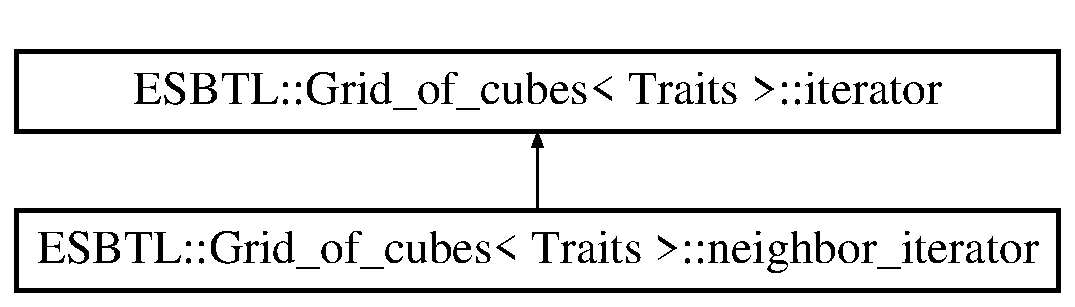
\includegraphics[height=2.000000cm]{classESBTL_1_1Grid__of__cubes_1_1neighbor__iterator}
\end{center}
\end{figure}
\subsection*{Public Member Functions}
\begin{DoxyCompactItemize}
\item 
\hyperlink{classESBTL_1_1Grid__of__cubes_1_1neighbor__iterator_a6d9db0dd9b4ea698dbfeb9edfb4e04ff}{neighbor\+\_\+iterator} ()
\item 
\hyperlink{classESBTL_1_1Grid__of__cubes_1_1neighbor__iterator_a6bd08cf90dc9bc48ba0ec6a209c5c1e2}{neighbor\+\_\+iterator} (const \hyperlink{structESBTL_1_1Grid__of__cubes_ad55c84346bab961e08d95e494551d07d}{Cube\+\_\+coordinates} \&C)
\item 
\hyperlink{classESBTL_1_1Grid__of__cubes_1_1neighbor__iterator_a6eaaee1feeb226221cb5711ea6242102}{neighbor\+\_\+iterator} (const \hyperlink{structESBTL_1_1Grid__of__cubes_ad55c84346bab961e08d95e494551d07d}{Cube\+\_\+coordinates} \&C, \hyperlink{structESBTL_1_1Grid__of__cubes}{Grid\+\_\+of\+\_\+cubes} $\ast$Grd)
\item 
\hyperlink{structESBTL_1_1Grid__of__cubes_ad55c84346bab961e08d95e494551d07d}{Cube\+\_\+coordinates} \& \hyperlink{classESBTL_1_1Grid__of__cubes_1_1neighbor__iterator_ac5e74d1983825788f0e80892b96c3517}{get\+\_\+current} ()
\item 
\hyperlink{classESBTL_1_1Grid__of__cubes_1_1neighbor__iterator}{neighbor\+\_\+iterator} \& \hyperlink{classESBTL_1_1Grid__of__cubes_1_1neighbor__iterator_a18641650d9d12e66224817deee861bc1}{operator++} ()
\end{DoxyCompactItemize}
\subsection*{Additional Inherited Members}


\subsection{Constructor \& Destructor Documentation}
\mbox{\Hypertarget{classESBTL_1_1Grid__of__cubes_1_1neighbor__iterator_a6d9db0dd9b4ea698dbfeb9edfb4e04ff}\label{classESBTL_1_1Grid__of__cubes_1_1neighbor__iterator_a6d9db0dd9b4ea698dbfeb9edfb4e04ff}} 
\index{E\+S\+B\+T\+L\+::\+Grid\+\_\+of\+\_\+cubes\+::neighbor\+\_\+iterator@{E\+S\+B\+T\+L\+::\+Grid\+\_\+of\+\_\+cubes\+::neighbor\+\_\+iterator}!neighbor\+\_\+iterator@{neighbor\+\_\+iterator}}
\index{neighbor\+\_\+iterator@{neighbor\+\_\+iterator}!E\+S\+B\+T\+L\+::\+Grid\+\_\+of\+\_\+cubes\+::neighbor\+\_\+iterator@{E\+S\+B\+T\+L\+::\+Grid\+\_\+of\+\_\+cubes\+::neighbor\+\_\+iterator}}
\subsubsection{\texorpdfstring{neighbor\+\_\+iterator()}{neighbor\_iterator()}\hspace{0.1cm}{\footnotesize\ttfamily [1/3]}}
{\footnotesize\ttfamily template$<$class Traits $>$ \\
\hyperlink{structESBTL_1_1Grid__of__cubes}{E\+S\+B\+T\+L\+::\+Grid\+\_\+of\+\_\+cubes}$<$ Traits $>$\+::neighbor\+\_\+iterator\+::neighbor\+\_\+iterator (\begin{DoxyParamCaption}{ }\end{DoxyParamCaption})\hspace{0.3cm}{\ttfamily [inline]}}

\mbox{\Hypertarget{classESBTL_1_1Grid__of__cubes_1_1neighbor__iterator_a6bd08cf90dc9bc48ba0ec6a209c5c1e2}\label{classESBTL_1_1Grid__of__cubes_1_1neighbor__iterator_a6bd08cf90dc9bc48ba0ec6a209c5c1e2}} 
\index{E\+S\+B\+T\+L\+::\+Grid\+\_\+of\+\_\+cubes\+::neighbor\+\_\+iterator@{E\+S\+B\+T\+L\+::\+Grid\+\_\+of\+\_\+cubes\+::neighbor\+\_\+iterator}!neighbor\+\_\+iterator@{neighbor\+\_\+iterator}}
\index{neighbor\+\_\+iterator@{neighbor\+\_\+iterator}!E\+S\+B\+T\+L\+::\+Grid\+\_\+of\+\_\+cubes\+::neighbor\+\_\+iterator@{E\+S\+B\+T\+L\+::\+Grid\+\_\+of\+\_\+cubes\+::neighbor\+\_\+iterator}}
\subsubsection{\texorpdfstring{neighbor\+\_\+iterator()}{neighbor\_iterator()}\hspace{0.1cm}{\footnotesize\ttfamily [2/3]}}
{\footnotesize\ttfamily template$<$class Traits $>$ \\
\hyperlink{structESBTL_1_1Grid__of__cubes}{E\+S\+B\+T\+L\+::\+Grid\+\_\+of\+\_\+cubes}$<$ Traits $>$\+::neighbor\+\_\+iterator\+::neighbor\+\_\+iterator (\begin{DoxyParamCaption}\item[{const \hyperlink{structESBTL_1_1Grid__of__cubes_ad55c84346bab961e08d95e494551d07d}{Cube\+\_\+coordinates} \&}]{C }\end{DoxyParamCaption})\hspace{0.3cm}{\ttfamily [inline]}}

\mbox{\Hypertarget{classESBTL_1_1Grid__of__cubes_1_1neighbor__iterator_a6eaaee1feeb226221cb5711ea6242102}\label{classESBTL_1_1Grid__of__cubes_1_1neighbor__iterator_a6eaaee1feeb226221cb5711ea6242102}} 
\index{E\+S\+B\+T\+L\+::\+Grid\+\_\+of\+\_\+cubes\+::neighbor\+\_\+iterator@{E\+S\+B\+T\+L\+::\+Grid\+\_\+of\+\_\+cubes\+::neighbor\+\_\+iterator}!neighbor\+\_\+iterator@{neighbor\+\_\+iterator}}
\index{neighbor\+\_\+iterator@{neighbor\+\_\+iterator}!E\+S\+B\+T\+L\+::\+Grid\+\_\+of\+\_\+cubes\+::neighbor\+\_\+iterator@{E\+S\+B\+T\+L\+::\+Grid\+\_\+of\+\_\+cubes\+::neighbor\+\_\+iterator}}
\subsubsection{\texorpdfstring{neighbor\+\_\+iterator()}{neighbor\_iterator()}\hspace{0.1cm}{\footnotesize\ttfamily [3/3]}}
{\footnotesize\ttfamily template$<$class Traits $>$ \\
\hyperlink{structESBTL_1_1Grid__of__cubes}{E\+S\+B\+T\+L\+::\+Grid\+\_\+of\+\_\+cubes}$<$ Traits $>$\+::neighbor\+\_\+iterator\+::neighbor\+\_\+iterator (\begin{DoxyParamCaption}\item[{const \hyperlink{structESBTL_1_1Grid__of__cubes_ad55c84346bab961e08d95e494551d07d}{Cube\+\_\+coordinates} \&}]{C,  }\item[{\hyperlink{structESBTL_1_1Grid__of__cubes}{Grid\+\_\+of\+\_\+cubes} $\ast$}]{Grd }\end{DoxyParamCaption})\hspace{0.3cm}{\ttfamily [inline]}}



\subsection{Member Function Documentation}
\mbox{\Hypertarget{classESBTL_1_1Grid__of__cubes_1_1neighbor__iterator_ac5e74d1983825788f0e80892b96c3517}\label{classESBTL_1_1Grid__of__cubes_1_1neighbor__iterator_ac5e74d1983825788f0e80892b96c3517}} 
\index{E\+S\+B\+T\+L\+::\+Grid\+\_\+of\+\_\+cubes\+::neighbor\+\_\+iterator@{E\+S\+B\+T\+L\+::\+Grid\+\_\+of\+\_\+cubes\+::neighbor\+\_\+iterator}!get\+\_\+current@{get\+\_\+current}}
\index{get\+\_\+current@{get\+\_\+current}!E\+S\+B\+T\+L\+::\+Grid\+\_\+of\+\_\+cubes\+::neighbor\+\_\+iterator@{E\+S\+B\+T\+L\+::\+Grid\+\_\+of\+\_\+cubes\+::neighbor\+\_\+iterator}}
\subsubsection{\texorpdfstring{get\+\_\+current()}{get\_current()}}
{\footnotesize\ttfamily template$<$class Traits $>$ \\
\hyperlink{structESBTL_1_1Grid__of__cubes_ad55c84346bab961e08d95e494551d07d}{Cube\+\_\+coordinates}\& \hyperlink{structESBTL_1_1Grid__of__cubes}{E\+S\+B\+T\+L\+::\+Grid\+\_\+of\+\_\+cubes}$<$ Traits $>$\+::neighbor\+\_\+iterator\+::get\+\_\+current (\begin{DoxyParamCaption}{ }\end{DoxyParamCaption})\hspace{0.3cm}{\ttfamily [inline]}}

\mbox{\Hypertarget{classESBTL_1_1Grid__of__cubes_1_1neighbor__iterator_a18641650d9d12e66224817deee861bc1}\label{classESBTL_1_1Grid__of__cubes_1_1neighbor__iterator_a18641650d9d12e66224817deee861bc1}} 
\index{E\+S\+B\+T\+L\+::\+Grid\+\_\+of\+\_\+cubes\+::neighbor\+\_\+iterator@{E\+S\+B\+T\+L\+::\+Grid\+\_\+of\+\_\+cubes\+::neighbor\+\_\+iterator}!operator++@{operator++}}
\index{operator++@{operator++}!E\+S\+B\+T\+L\+::\+Grid\+\_\+of\+\_\+cubes\+::neighbor\+\_\+iterator@{E\+S\+B\+T\+L\+::\+Grid\+\_\+of\+\_\+cubes\+::neighbor\+\_\+iterator}}
\subsubsection{\texorpdfstring{operator++()}{operator++()}}
{\footnotesize\ttfamily template$<$class Traits $>$ \\
\hyperlink{classESBTL_1_1Grid__of__cubes_1_1neighbor__iterator}{neighbor\+\_\+iterator}\& \hyperlink{structESBTL_1_1Grid__of__cubes}{E\+S\+B\+T\+L\+::\+Grid\+\_\+of\+\_\+cubes}$<$ Traits $>$\+::neighbor\+\_\+iterator\+::operator++ (\begin{DoxyParamCaption}{ }\end{DoxyParamCaption})\hspace{0.3cm}{\ttfamily [inline]}}



The documentation for this class was generated from the following file\+:\begin{DoxyCompactItemize}
\item 
\hyperlink{grid__of__cubes_8h}{grid\+\_\+of\+\_\+cubes.\+h}\end{DoxyCompactItemize}

\hypertarget{structESBTL_1_1No__occupancy__policy}{}\section{E\+S\+B\+TL\+:\+:No\+\_\+occupancy\+\_\+policy$<$ Line\+\_\+format $>$ Struct Template Reference}
\label{structESBTL_1_1No__occupancy__policy}\index{E\+S\+B\+T\+L\+::\+No\+\_\+occupancy\+\_\+policy$<$ Line\+\_\+format $>$@{E\+S\+B\+T\+L\+::\+No\+\_\+occupancy\+\_\+policy$<$ Line\+\_\+format $>$}}


{\ttfamily \#include $<$occupancy\+\_\+handlers.\+h$>$}

\subsection*{Public Member Functions}
\begin{DoxyCompactItemize}
\item 
int \hyperlink{structESBTL_1_1No__occupancy__policy_ae3d1ae3f42e09e938787e349f43b078b}{add\+\_\+or\+\_\+postpone} (const Line\+\_\+format \&line\+\_\+format, const std\+::string \&line, int system\+\_\+index) const
\item 
{\footnotesize template$<$class Builder $>$ }\\int \hyperlink{structESBTL_1_1No__occupancy__policy_aa8cf0b10f6df8b195d50a0b120784799}{finalize} (Builder \&) const
\end{DoxyCompactItemize}


\subsection{Detailed Description}
\subsubsection*{template$<$class Line\+\_\+format$>$\newline
struct E\+S\+B\+T\+L\+::\+No\+\_\+occupancy\+\_\+policy$<$ Line\+\_\+format $>$}

This object provides no occupancy policy. This results in a crash of the application when an atom with no alternate location and with occupancy!=1 is encountered. 
\begin{DoxyTemplParams}{Template Parameters}
{\em Line\+\_\+format} & is a helper class to read molecular data files such as \hyperlink{classESBTL_1_1PDB_1_1Line__format}{E\+S\+B\+T\+L\+::\+P\+D\+B\+::\+Line\+\_\+format}. \\
\hline
\end{DoxyTemplParams}


\subsection{Member Function Documentation}
\mbox{\Hypertarget{structESBTL_1_1No__occupancy__policy_ae3d1ae3f42e09e938787e349f43b078b}\label{structESBTL_1_1No__occupancy__policy_ae3d1ae3f42e09e938787e349f43b078b}} 
\index{E\+S\+B\+T\+L\+::\+No\+\_\+occupancy\+\_\+policy@{E\+S\+B\+T\+L\+::\+No\+\_\+occupancy\+\_\+policy}!add\+\_\+or\+\_\+postpone@{add\+\_\+or\+\_\+postpone}}
\index{add\+\_\+or\+\_\+postpone@{add\+\_\+or\+\_\+postpone}!E\+S\+B\+T\+L\+::\+No\+\_\+occupancy\+\_\+policy@{E\+S\+B\+T\+L\+::\+No\+\_\+occupancy\+\_\+policy}}
\subsubsection{\texorpdfstring{add\+\_\+or\+\_\+postpone()}{add\_or\_postpone()}}
{\footnotesize\ttfamily template$<$class Line\+\_\+format $>$ \\
int \hyperlink{structESBTL_1_1No__occupancy__policy}{E\+S\+B\+T\+L\+::\+No\+\_\+occupancy\+\_\+policy}$<$ Line\+\_\+format $>$\+::add\+\_\+or\+\_\+postpone (\begin{DoxyParamCaption}\item[{const Line\+\_\+format \&}]{line\+\_\+format,  }\item[{const std\+::string \&}]{line,  }\item[{int}]{system\+\_\+index }\end{DoxyParamCaption}) const\hspace{0.3cm}{\ttfamily [inline]}}

\mbox{\Hypertarget{structESBTL_1_1No__occupancy__policy_aa8cf0b10f6df8b195d50a0b120784799}\label{structESBTL_1_1No__occupancy__policy_aa8cf0b10f6df8b195d50a0b120784799}} 
\index{E\+S\+B\+T\+L\+::\+No\+\_\+occupancy\+\_\+policy@{E\+S\+B\+T\+L\+::\+No\+\_\+occupancy\+\_\+policy}!finalize@{finalize}}
\index{finalize@{finalize}!E\+S\+B\+T\+L\+::\+No\+\_\+occupancy\+\_\+policy@{E\+S\+B\+T\+L\+::\+No\+\_\+occupancy\+\_\+policy}}
\subsubsection{\texorpdfstring{finalize()}{finalize()}}
{\footnotesize\ttfamily template$<$class Line\+\_\+format $>$ \\
template$<$class Builder $>$ \\
int \hyperlink{structESBTL_1_1No__occupancy__policy}{E\+S\+B\+T\+L\+::\+No\+\_\+occupancy\+\_\+policy}$<$ Line\+\_\+format $>$\+::finalize (\begin{DoxyParamCaption}\item[{Builder \&}]{ }\end{DoxyParamCaption}) const\hspace{0.3cm}{\ttfamily [inline]}}



The documentation for this struct was generated from the following file\+:\begin{DoxyCompactItemize}
\item 
\hyperlink{occupancy__handlers_8h}{occupancy\+\_\+handlers.\+h}\end{DoxyCompactItemize}

\hypertarget{structESBTL_1_1Not__functor}{}\section{E\+S\+B\+TL\+:\+:Not\+\_\+functor$<$ S $>$ Struct Template Reference}
\label{structESBTL_1_1Not__functor}\index{E\+S\+B\+T\+L\+::\+Not\+\_\+functor$<$ S $>$@{E\+S\+B\+T\+L\+::\+Not\+\_\+functor$<$ S $>$}}


{\ttfamily \#include $<$combine\+\_\+boolean\+\_\+operator.\+h$>$}

Inheritance diagram for E\+S\+B\+TL\+:\+:Not\+\_\+functor$<$ S $>$\+:\begin{figure}[H]
\begin{center}
\leavevmode
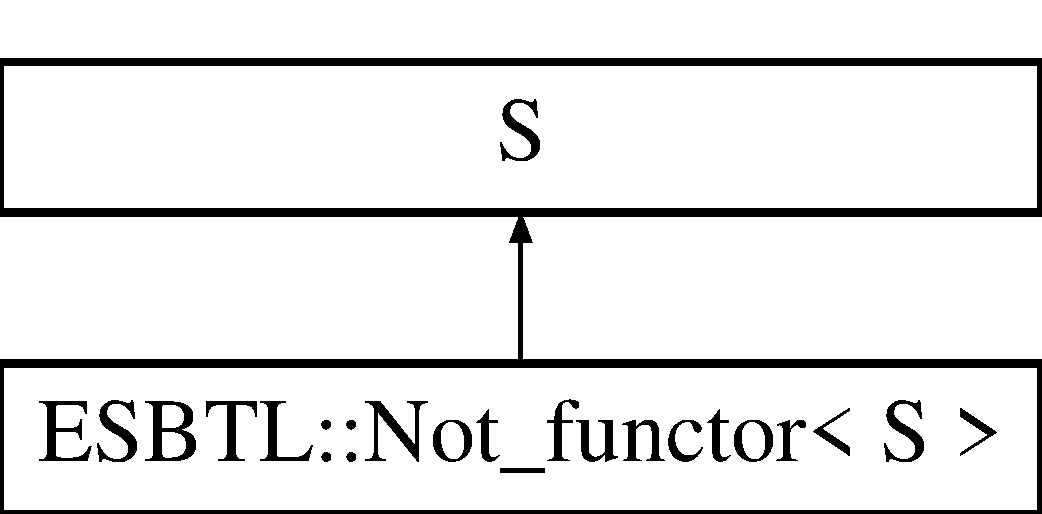
\includegraphics[height=2.000000cm]{structESBTL_1_1Not__functor}
\end{center}
\end{figure}
\subsection*{Public Member Functions}
\begin{DoxyCompactItemize}
\item 
\hyperlink{structESBTL_1_1Not__functor_a33d2670f7406276a8690e65bd1e5a6f7}{Not\+\_\+functor} ()
\item 
\hyperlink{structESBTL_1_1Not__functor_aab72e39a6e57edad9f2c15e59ec34836}{Not\+\_\+functor} (const S \&s)
\item 
{\footnotesize template$<$class T $>$ }\\bool \hyperlink{structESBTL_1_1Not__functor_a207c726758b2318efe580dd948d4d7a5}{operator()} (const T \&t) const
\end{DoxyCompactItemize}


\subsection{Detailed Description}
\subsubsection*{template$<$class S$>$\newline
struct E\+S\+B\+T\+L\+::\+Not\+\_\+functor$<$ S $>$}

Class defining a function object returning the opposite result of a given function object. 
\begin{DoxyTemplParams}{Template Parameters}
{\em S} & is a function object with an operator() taking one argument and returning a Boolean (such as \hyperlink{group__atomsel}{Atom selection}). \\
\hline
\end{DoxyTemplParams}


\subsection{Constructor \& Destructor Documentation}
\mbox{\Hypertarget{structESBTL_1_1Not__functor_a33d2670f7406276a8690e65bd1e5a6f7}\label{structESBTL_1_1Not__functor_a33d2670f7406276a8690e65bd1e5a6f7}} 
\index{E\+S\+B\+T\+L\+::\+Not\+\_\+functor@{E\+S\+B\+T\+L\+::\+Not\+\_\+functor}!Not\+\_\+functor@{Not\+\_\+functor}}
\index{Not\+\_\+functor@{Not\+\_\+functor}!E\+S\+B\+T\+L\+::\+Not\+\_\+functor@{E\+S\+B\+T\+L\+::\+Not\+\_\+functor}}
\subsubsection{\texorpdfstring{Not\+\_\+functor()}{Not\_functor()}\hspace{0.1cm}{\footnotesize\ttfamily [1/2]}}
{\footnotesize\ttfamily template$<$class S $>$ \\
\hyperlink{structESBTL_1_1Not__functor}{E\+S\+B\+T\+L\+::\+Not\+\_\+functor}$<$ S $>$\+::\hyperlink{structESBTL_1_1Not__functor}{Not\+\_\+functor} (\begin{DoxyParamCaption}{ }\end{DoxyParamCaption})\hspace{0.3cm}{\ttfamily [inline]}}

\mbox{\Hypertarget{structESBTL_1_1Not__functor_aab72e39a6e57edad9f2c15e59ec34836}\label{structESBTL_1_1Not__functor_aab72e39a6e57edad9f2c15e59ec34836}} 
\index{E\+S\+B\+T\+L\+::\+Not\+\_\+functor@{E\+S\+B\+T\+L\+::\+Not\+\_\+functor}!Not\+\_\+functor@{Not\+\_\+functor}}
\index{Not\+\_\+functor@{Not\+\_\+functor}!E\+S\+B\+T\+L\+::\+Not\+\_\+functor@{E\+S\+B\+T\+L\+::\+Not\+\_\+functor}}
\subsubsection{\texorpdfstring{Not\+\_\+functor()}{Not\_functor()}\hspace{0.1cm}{\footnotesize\ttfamily [2/2]}}
{\footnotesize\ttfamily template$<$class S $>$ \\
\hyperlink{structESBTL_1_1Not__functor}{E\+S\+B\+T\+L\+::\+Not\+\_\+functor}$<$ S $>$\+::\hyperlink{structESBTL_1_1Not__functor}{Not\+\_\+functor} (\begin{DoxyParamCaption}\item[{const S \&}]{s }\end{DoxyParamCaption})\hspace{0.3cm}{\ttfamily [inline]}}



\subsection{Member Function Documentation}
\mbox{\Hypertarget{structESBTL_1_1Not__functor_a207c726758b2318efe580dd948d4d7a5}\label{structESBTL_1_1Not__functor_a207c726758b2318efe580dd948d4d7a5}} 
\index{E\+S\+B\+T\+L\+::\+Not\+\_\+functor@{E\+S\+B\+T\+L\+::\+Not\+\_\+functor}!operator()@{operator()}}
\index{operator()@{operator()}!E\+S\+B\+T\+L\+::\+Not\+\_\+functor@{E\+S\+B\+T\+L\+::\+Not\+\_\+functor}}
\subsubsection{\texorpdfstring{operator()()}{operator()()}}
{\footnotesize\ttfamily template$<$class S $>$ \\
template$<$class T $>$ \\
bool \hyperlink{structESBTL_1_1Not__functor}{E\+S\+B\+T\+L\+::\+Not\+\_\+functor}$<$ S $>$\+::operator() (\begin{DoxyParamCaption}\item[{const T \&}]{t }\end{DoxyParamCaption}) const\hspace{0.3cm}{\ttfamily [inline]}}



The documentation for this struct was generated from the following file\+:\begin{DoxyCompactItemize}
\item 
\hyperlink{combine__boolean__operator_8h}{combine\+\_\+boolean\+\_\+operator.\+h}\end{DoxyCompactItemize}

\hypertarget{classESBTL_1_1Grid__of__cubes_1_1object__iterator}{}\section{E\+S\+B\+TL\+:\+:Grid\+\_\+of\+\_\+cubes$<$ Traits $>$\+:\+:object\+\_\+iterator Class Reference}
\label{classESBTL_1_1Grid__of__cubes_1_1object__iterator}\index{E\+S\+B\+T\+L\+::\+Grid\+\_\+of\+\_\+cubes$<$ Traits $>$\+::object\+\_\+iterator@{E\+S\+B\+T\+L\+::\+Grid\+\_\+of\+\_\+cubes$<$ Traits $>$\+::object\+\_\+iterator}}


{\ttfamily \#include $<$grid\+\_\+of\+\_\+cubes.\+h$>$}

\subsection*{Public Member Functions}
\begin{DoxyCompactItemize}
\item 
\hyperlink{classESBTL_1_1Grid__of__cubes_1_1object__iterator_ade271a0528949eaafd1d132e923d51d3}{object\+\_\+iterator} ()
\item 
\hyperlink{classESBTL_1_1Grid__of__cubes_1_1object__iterator_abaa8b1c0c35d741a1b890990f5a53c14}{object\+\_\+iterator} (\hyperlink{classESBTL_1_1Grid__of__cubes_1_1iterator}{iterator} it, \hyperlink{structESBTL_1_1Grid__of__cubes_a1586dac85e561a73b591da3cf07a47b1}{In\+\_\+cube\+\_\+iterator} itc)
\item 
\hyperlink{classESBTL_1_1Grid__of__cubes_1_1object__iterator_ab31b4d094b8975e5588e8b7cd0c8115b}{object\+\_\+iterator} (\hyperlink{classESBTL_1_1Grid__of__cubes_1_1iterator}{iterator} it)
\item 
\hyperlink{classESBTL_1_1Grid__of__cubes_1_1object__iterator}{object\+\_\+iterator} \& \hyperlink{classESBTL_1_1Grid__of__cubes_1_1object__iterator_ae9b040a5ef31ab3d809417d124868263}{operator++} ()
\item 
\hyperlink{classESBTL_1_1Grid__of__cubes_1_1object__iterator}{object\+\_\+iterator} \hyperlink{classESBTL_1_1Grid__of__cubes_1_1object__iterator_afafc104603aabb65ab4c85c3731b1e6a}{operator++} (int)
\item 
\hyperlink{structESBTL_1_1Grid__of__cubes_ae77665f05d6c7ae05c3d2d764df99193}{Object\+\_\+iterator} \& \hyperlink{classESBTL_1_1Grid__of__cubes_1_1object__iterator_aa037306d61ffcf82aa0c88d3df470872}{operator$\ast$} ()
\item 
\hyperlink{structESBTL_1_1Grid__of__cubes_1_1Cube__unit}{Cube\+\_\+unit} $\ast$ \hyperlink{classESBTL_1_1Grid__of__cubes_1_1object__iterator_a4c50c8eb4de7ca977382405d39d51ae8}{operator-\/$>$} ()
\item 
bool \hyperlink{classESBTL_1_1Grid__of__cubes_1_1object__iterator_a715d66fdedfae22f18c85aa14aada3e1}{operator==} (const \hyperlink{classESBTL_1_1Grid__of__cubes_1_1object__iterator}{object\+\_\+iterator} \&it)
\item 
bool \hyperlink{classESBTL_1_1Grid__of__cubes_1_1object__iterator_a7f43e1c35ee8287612cd4db94d923f56}{operator!=} (const \hyperlink{classESBTL_1_1Grid__of__cubes_1_1object__iterator}{object\+\_\+iterator} \&it)
\end{DoxyCompactItemize}
\subsection*{Protected Attributes}
\begin{DoxyCompactItemize}
\item 
\hyperlink{classESBTL_1_1Grid__of__cubes_1_1iterator}{iterator} \hyperlink{classESBTL_1_1Grid__of__cubes_1_1object__iterator_abdd1562be62c036e6b6ef1c7fe331d24}{current\+\_\+cube}
\item 
\hyperlink{structESBTL_1_1Grid__of__cubes_a1586dac85e561a73b591da3cf07a47b1}{In\+\_\+cube\+\_\+iterator} \hyperlink{classESBTL_1_1Grid__of__cubes_1_1object__iterator_a80eb9046339bde86d3978c55f3578d5f}{current\+\_\+object}
\end{DoxyCompactItemize}
\subsection*{Friends}
\begin{DoxyCompactItemize}
\item 
void \hyperlink{classESBTL_1_1Grid__of__cubes_1_1object__iterator_a34522cc0511a0818c99ebcd4d1f010ec}{Grid\+\_\+of\+\_\+cubes} (const \hyperlink{classESBTL_1_1Grid__of__cubes_1_1object__iterator}{object\+\_\+iterator} \&it)
\end{DoxyCompactItemize}


\subsection{Constructor \& Destructor Documentation}
\mbox{\Hypertarget{classESBTL_1_1Grid__of__cubes_1_1object__iterator_ade271a0528949eaafd1d132e923d51d3}\label{classESBTL_1_1Grid__of__cubes_1_1object__iterator_ade271a0528949eaafd1d132e923d51d3}} 
\index{E\+S\+B\+T\+L\+::\+Grid\+\_\+of\+\_\+cubes\+::object\+\_\+iterator@{E\+S\+B\+T\+L\+::\+Grid\+\_\+of\+\_\+cubes\+::object\+\_\+iterator}!object\+\_\+iterator@{object\+\_\+iterator}}
\index{object\+\_\+iterator@{object\+\_\+iterator}!E\+S\+B\+T\+L\+::\+Grid\+\_\+of\+\_\+cubes\+::object\+\_\+iterator@{E\+S\+B\+T\+L\+::\+Grid\+\_\+of\+\_\+cubes\+::object\+\_\+iterator}}
\subsubsection{\texorpdfstring{object\+\_\+iterator()}{object\_iterator()}\hspace{0.1cm}{\footnotesize\ttfamily [1/3]}}
{\footnotesize\ttfamily template$<$class Traits $>$ \\
\hyperlink{structESBTL_1_1Grid__of__cubes}{E\+S\+B\+T\+L\+::\+Grid\+\_\+of\+\_\+cubes}$<$ Traits $>$\+::object\+\_\+iterator\+::object\+\_\+iterator (\begin{DoxyParamCaption}{ }\end{DoxyParamCaption})\hspace{0.3cm}{\ttfamily [inline]}}

\mbox{\Hypertarget{classESBTL_1_1Grid__of__cubes_1_1object__iterator_abaa8b1c0c35d741a1b890990f5a53c14}\label{classESBTL_1_1Grid__of__cubes_1_1object__iterator_abaa8b1c0c35d741a1b890990f5a53c14}} 
\index{E\+S\+B\+T\+L\+::\+Grid\+\_\+of\+\_\+cubes\+::object\+\_\+iterator@{E\+S\+B\+T\+L\+::\+Grid\+\_\+of\+\_\+cubes\+::object\+\_\+iterator}!object\+\_\+iterator@{object\+\_\+iterator}}
\index{object\+\_\+iterator@{object\+\_\+iterator}!E\+S\+B\+T\+L\+::\+Grid\+\_\+of\+\_\+cubes\+::object\+\_\+iterator@{E\+S\+B\+T\+L\+::\+Grid\+\_\+of\+\_\+cubes\+::object\+\_\+iterator}}
\subsubsection{\texorpdfstring{object\+\_\+iterator()}{object\_iterator()}\hspace{0.1cm}{\footnotesize\ttfamily [2/3]}}
{\footnotesize\ttfamily template$<$class Traits $>$ \\
\hyperlink{structESBTL_1_1Grid__of__cubes}{E\+S\+B\+T\+L\+::\+Grid\+\_\+of\+\_\+cubes}$<$ Traits $>$\+::object\+\_\+iterator\+::object\+\_\+iterator (\begin{DoxyParamCaption}\item[{\hyperlink{classESBTL_1_1Grid__of__cubes_1_1iterator}{iterator}}]{it,  }\item[{\hyperlink{structESBTL_1_1Grid__of__cubes_a1586dac85e561a73b591da3cf07a47b1}{In\+\_\+cube\+\_\+iterator}}]{itc }\end{DoxyParamCaption})\hspace{0.3cm}{\ttfamily [inline]}}

\mbox{\Hypertarget{classESBTL_1_1Grid__of__cubes_1_1object__iterator_ab31b4d094b8975e5588e8b7cd0c8115b}\label{classESBTL_1_1Grid__of__cubes_1_1object__iterator_ab31b4d094b8975e5588e8b7cd0c8115b}} 
\index{E\+S\+B\+T\+L\+::\+Grid\+\_\+of\+\_\+cubes\+::object\+\_\+iterator@{E\+S\+B\+T\+L\+::\+Grid\+\_\+of\+\_\+cubes\+::object\+\_\+iterator}!object\+\_\+iterator@{object\+\_\+iterator}}
\index{object\+\_\+iterator@{object\+\_\+iterator}!E\+S\+B\+T\+L\+::\+Grid\+\_\+of\+\_\+cubes\+::object\+\_\+iterator@{E\+S\+B\+T\+L\+::\+Grid\+\_\+of\+\_\+cubes\+::object\+\_\+iterator}}
\subsubsection{\texorpdfstring{object\+\_\+iterator()}{object\_iterator()}\hspace{0.1cm}{\footnotesize\ttfamily [3/3]}}
{\footnotesize\ttfamily template$<$class Traits $>$ \\
\hyperlink{structESBTL_1_1Grid__of__cubes}{E\+S\+B\+T\+L\+::\+Grid\+\_\+of\+\_\+cubes}$<$ Traits $>$\+::object\+\_\+iterator\+::object\+\_\+iterator (\begin{DoxyParamCaption}\item[{\hyperlink{classESBTL_1_1Grid__of__cubes_1_1iterator}{iterator}}]{it }\end{DoxyParamCaption})\hspace{0.3cm}{\ttfamily [inline]}}



\subsection{Member Function Documentation}
\mbox{\Hypertarget{classESBTL_1_1Grid__of__cubes_1_1object__iterator_a7f43e1c35ee8287612cd4db94d923f56}\label{classESBTL_1_1Grid__of__cubes_1_1object__iterator_a7f43e1c35ee8287612cd4db94d923f56}} 
\index{E\+S\+B\+T\+L\+::\+Grid\+\_\+of\+\_\+cubes\+::object\+\_\+iterator@{E\+S\+B\+T\+L\+::\+Grid\+\_\+of\+\_\+cubes\+::object\+\_\+iterator}!operator"!=@{operator"!=}}
\index{operator"!=@{operator"!=}!E\+S\+B\+T\+L\+::\+Grid\+\_\+of\+\_\+cubes\+::object\+\_\+iterator@{E\+S\+B\+T\+L\+::\+Grid\+\_\+of\+\_\+cubes\+::object\+\_\+iterator}}
\subsubsection{\texorpdfstring{operator"!=()}{operator!=()}}
{\footnotesize\ttfamily template$<$class Traits $>$ \\
bool \hyperlink{structESBTL_1_1Grid__of__cubes}{E\+S\+B\+T\+L\+::\+Grid\+\_\+of\+\_\+cubes}$<$ Traits $>$\+::object\+\_\+iterator\+::operator!= (\begin{DoxyParamCaption}\item[{const \hyperlink{classESBTL_1_1Grid__of__cubes_1_1object__iterator}{object\+\_\+iterator} \&}]{it }\end{DoxyParamCaption})\hspace{0.3cm}{\ttfamily [inline]}}

\mbox{\Hypertarget{classESBTL_1_1Grid__of__cubes_1_1object__iterator_aa037306d61ffcf82aa0c88d3df470872}\label{classESBTL_1_1Grid__of__cubes_1_1object__iterator_aa037306d61ffcf82aa0c88d3df470872}} 
\index{E\+S\+B\+T\+L\+::\+Grid\+\_\+of\+\_\+cubes\+::object\+\_\+iterator@{E\+S\+B\+T\+L\+::\+Grid\+\_\+of\+\_\+cubes\+::object\+\_\+iterator}!operator$\ast$@{operator$\ast$}}
\index{operator$\ast$@{operator$\ast$}!E\+S\+B\+T\+L\+::\+Grid\+\_\+of\+\_\+cubes\+::object\+\_\+iterator@{E\+S\+B\+T\+L\+::\+Grid\+\_\+of\+\_\+cubes\+::object\+\_\+iterator}}
\subsubsection{\texorpdfstring{operator$\ast$()}{operator*()}}
{\footnotesize\ttfamily template$<$class Traits $>$ \\
\hyperlink{structESBTL_1_1Grid__of__cubes_ae77665f05d6c7ae05c3d2d764df99193}{Object\+\_\+iterator}\& \hyperlink{structESBTL_1_1Grid__of__cubes}{E\+S\+B\+T\+L\+::\+Grid\+\_\+of\+\_\+cubes}$<$ Traits $>$\+::object\+\_\+iterator\+::operator$\ast$ (\begin{DoxyParamCaption}{ }\end{DoxyParamCaption})\hspace{0.3cm}{\ttfamily [inline]}}

\mbox{\Hypertarget{classESBTL_1_1Grid__of__cubes_1_1object__iterator_ae9b040a5ef31ab3d809417d124868263}\label{classESBTL_1_1Grid__of__cubes_1_1object__iterator_ae9b040a5ef31ab3d809417d124868263}} 
\index{E\+S\+B\+T\+L\+::\+Grid\+\_\+of\+\_\+cubes\+::object\+\_\+iterator@{E\+S\+B\+T\+L\+::\+Grid\+\_\+of\+\_\+cubes\+::object\+\_\+iterator}!operator++@{operator++}}
\index{operator++@{operator++}!E\+S\+B\+T\+L\+::\+Grid\+\_\+of\+\_\+cubes\+::object\+\_\+iterator@{E\+S\+B\+T\+L\+::\+Grid\+\_\+of\+\_\+cubes\+::object\+\_\+iterator}}
\subsubsection{\texorpdfstring{operator++()}{operator++()}\hspace{0.1cm}{\footnotesize\ttfamily [1/2]}}
{\footnotesize\ttfamily template$<$class Traits $>$ \\
\hyperlink{classESBTL_1_1Grid__of__cubes_1_1object__iterator}{object\+\_\+iterator}\& \hyperlink{structESBTL_1_1Grid__of__cubes}{E\+S\+B\+T\+L\+::\+Grid\+\_\+of\+\_\+cubes}$<$ Traits $>$\+::object\+\_\+iterator\+::operator++ (\begin{DoxyParamCaption}{ }\end{DoxyParamCaption})\hspace{0.3cm}{\ttfamily [inline]}}

\mbox{\Hypertarget{classESBTL_1_1Grid__of__cubes_1_1object__iterator_afafc104603aabb65ab4c85c3731b1e6a}\label{classESBTL_1_1Grid__of__cubes_1_1object__iterator_afafc104603aabb65ab4c85c3731b1e6a}} 
\index{E\+S\+B\+T\+L\+::\+Grid\+\_\+of\+\_\+cubes\+::object\+\_\+iterator@{E\+S\+B\+T\+L\+::\+Grid\+\_\+of\+\_\+cubes\+::object\+\_\+iterator}!operator++@{operator++}}
\index{operator++@{operator++}!E\+S\+B\+T\+L\+::\+Grid\+\_\+of\+\_\+cubes\+::object\+\_\+iterator@{E\+S\+B\+T\+L\+::\+Grid\+\_\+of\+\_\+cubes\+::object\+\_\+iterator}}
\subsubsection{\texorpdfstring{operator++()}{operator++()}\hspace{0.1cm}{\footnotesize\ttfamily [2/2]}}
{\footnotesize\ttfamily template$<$class Traits $>$ \\
\hyperlink{classESBTL_1_1Grid__of__cubes_1_1object__iterator}{object\+\_\+iterator} \hyperlink{structESBTL_1_1Grid__of__cubes}{E\+S\+B\+T\+L\+::\+Grid\+\_\+of\+\_\+cubes}$<$ Traits $>$\+::object\+\_\+iterator\+::operator++ (\begin{DoxyParamCaption}\item[{int}]{ }\end{DoxyParamCaption})\hspace{0.3cm}{\ttfamily [inline]}}

\mbox{\Hypertarget{classESBTL_1_1Grid__of__cubes_1_1object__iterator_a4c50c8eb4de7ca977382405d39d51ae8}\label{classESBTL_1_1Grid__of__cubes_1_1object__iterator_a4c50c8eb4de7ca977382405d39d51ae8}} 
\index{E\+S\+B\+T\+L\+::\+Grid\+\_\+of\+\_\+cubes\+::object\+\_\+iterator@{E\+S\+B\+T\+L\+::\+Grid\+\_\+of\+\_\+cubes\+::object\+\_\+iterator}!operator-\/$>$@{operator-\/$>$}}
\index{operator-\/$>$@{operator-\/$>$}!E\+S\+B\+T\+L\+::\+Grid\+\_\+of\+\_\+cubes\+::object\+\_\+iterator@{E\+S\+B\+T\+L\+::\+Grid\+\_\+of\+\_\+cubes\+::object\+\_\+iterator}}
\subsubsection{\texorpdfstring{operator-\/$>$()}{operator->()}}
{\footnotesize\ttfamily template$<$class Traits $>$ \\
\hyperlink{structESBTL_1_1Grid__of__cubes_1_1Cube__unit}{Cube\+\_\+unit}$\ast$ \hyperlink{structESBTL_1_1Grid__of__cubes}{E\+S\+B\+T\+L\+::\+Grid\+\_\+of\+\_\+cubes}$<$ Traits $>$\+::object\+\_\+iterator\+::operator-\/$>$ (\begin{DoxyParamCaption}{ }\end{DoxyParamCaption})\hspace{0.3cm}{\ttfamily [inline]}}

\mbox{\Hypertarget{classESBTL_1_1Grid__of__cubes_1_1object__iterator_a715d66fdedfae22f18c85aa14aada3e1}\label{classESBTL_1_1Grid__of__cubes_1_1object__iterator_a715d66fdedfae22f18c85aa14aada3e1}} 
\index{E\+S\+B\+T\+L\+::\+Grid\+\_\+of\+\_\+cubes\+::object\+\_\+iterator@{E\+S\+B\+T\+L\+::\+Grid\+\_\+of\+\_\+cubes\+::object\+\_\+iterator}!operator==@{operator==}}
\index{operator==@{operator==}!E\+S\+B\+T\+L\+::\+Grid\+\_\+of\+\_\+cubes\+::object\+\_\+iterator@{E\+S\+B\+T\+L\+::\+Grid\+\_\+of\+\_\+cubes\+::object\+\_\+iterator}}
\subsubsection{\texorpdfstring{operator==()}{operator==()}}
{\footnotesize\ttfamily template$<$class Traits $>$ \\
bool \hyperlink{structESBTL_1_1Grid__of__cubes}{E\+S\+B\+T\+L\+::\+Grid\+\_\+of\+\_\+cubes}$<$ Traits $>$\+::object\+\_\+iterator\+::operator== (\begin{DoxyParamCaption}\item[{const \hyperlink{classESBTL_1_1Grid__of__cubes_1_1object__iterator}{object\+\_\+iterator} \&}]{it }\end{DoxyParamCaption})\hspace{0.3cm}{\ttfamily [inline]}}



\subsection{Friends And Related Function Documentation}
\mbox{\Hypertarget{classESBTL_1_1Grid__of__cubes_1_1object__iterator_a34522cc0511a0818c99ebcd4d1f010ec}\label{classESBTL_1_1Grid__of__cubes_1_1object__iterator_a34522cc0511a0818c99ebcd4d1f010ec}} 
\index{E\+S\+B\+T\+L\+::\+Grid\+\_\+of\+\_\+cubes\+::object\+\_\+iterator@{E\+S\+B\+T\+L\+::\+Grid\+\_\+of\+\_\+cubes\+::object\+\_\+iterator}!Grid\+\_\+of\+\_\+cubes@{Grid\+\_\+of\+\_\+cubes}}
\index{Grid\+\_\+of\+\_\+cubes@{Grid\+\_\+of\+\_\+cubes}!E\+S\+B\+T\+L\+::\+Grid\+\_\+of\+\_\+cubes\+::object\+\_\+iterator@{E\+S\+B\+T\+L\+::\+Grid\+\_\+of\+\_\+cubes\+::object\+\_\+iterator}}
\subsubsection{\texorpdfstring{Grid\+\_\+of\+\_\+cubes}{Grid\_of\_cubes}}
{\footnotesize\ttfamily template$<$class Traits $>$ \\
void \hyperlink{structESBTL_1_1Grid__of__cubes}{Grid\+\_\+of\+\_\+cubes} (\begin{DoxyParamCaption}\item[{const \hyperlink{classESBTL_1_1Grid__of__cubes_1_1object__iterator}{object\+\_\+iterator} \&}]{it }\end{DoxyParamCaption})\hspace{0.3cm}{\ttfamily [friend]}}



\subsection{Member Data Documentation}
\mbox{\Hypertarget{classESBTL_1_1Grid__of__cubes_1_1object__iterator_abdd1562be62c036e6b6ef1c7fe331d24}\label{classESBTL_1_1Grid__of__cubes_1_1object__iterator_abdd1562be62c036e6b6ef1c7fe331d24}} 
\index{E\+S\+B\+T\+L\+::\+Grid\+\_\+of\+\_\+cubes\+::object\+\_\+iterator@{E\+S\+B\+T\+L\+::\+Grid\+\_\+of\+\_\+cubes\+::object\+\_\+iterator}!current\+\_\+cube@{current\+\_\+cube}}
\index{current\+\_\+cube@{current\+\_\+cube}!E\+S\+B\+T\+L\+::\+Grid\+\_\+of\+\_\+cubes\+::object\+\_\+iterator@{E\+S\+B\+T\+L\+::\+Grid\+\_\+of\+\_\+cubes\+::object\+\_\+iterator}}
\subsubsection{\texorpdfstring{current\+\_\+cube}{current\_cube}}
{\footnotesize\ttfamily template$<$class Traits $>$ \\
\hyperlink{classESBTL_1_1Grid__of__cubes_1_1iterator}{iterator} \hyperlink{structESBTL_1_1Grid__of__cubes}{E\+S\+B\+T\+L\+::\+Grid\+\_\+of\+\_\+cubes}$<$ Traits $>$\+::object\+\_\+iterator\+::current\+\_\+cube\hspace{0.3cm}{\ttfamily [protected]}}

\mbox{\Hypertarget{classESBTL_1_1Grid__of__cubes_1_1object__iterator_a80eb9046339bde86d3978c55f3578d5f}\label{classESBTL_1_1Grid__of__cubes_1_1object__iterator_a80eb9046339bde86d3978c55f3578d5f}} 
\index{E\+S\+B\+T\+L\+::\+Grid\+\_\+of\+\_\+cubes\+::object\+\_\+iterator@{E\+S\+B\+T\+L\+::\+Grid\+\_\+of\+\_\+cubes\+::object\+\_\+iterator}!current\+\_\+object@{current\+\_\+object}}
\index{current\+\_\+object@{current\+\_\+object}!E\+S\+B\+T\+L\+::\+Grid\+\_\+of\+\_\+cubes\+::object\+\_\+iterator@{E\+S\+B\+T\+L\+::\+Grid\+\_\+of\+\_\+cubes\+::object\+\_\+iterator}}
\subsubsection{\texorpdfstring{current\+\_\+object}{current\_object}}
{\footnotesize\ttfamily template$<$class Traits $>$ \\
\hyperlink{structESBTL_1_1Grid__of__cubes_a1586dac85e561a73b591da3cf07a47b1}{In\+\_\+cube\+\_\+iterator} \hyperlink{structESBTL_1_1Grid__of__cubes}{E\+S\+B\+T\+L\+::\+Grid\+\_\+of\+\_\+cubes}$<$ Traits $>$\+::object\+\_\+iterator\+::current\+\_\+object\hspace{0.3cm}{\ttfamily [protected]}}



The documentation for this class was generated from the following file\+:\begin{DoxyCompactItemize}
\item 
\hyperlink{grid__of__cubes_8h}{grid\+\_\+of\+\_\+cubes.\+h}\end{DoxyCompactItemize}

\hypertarget{classESBTL_1_1Or__functors}{}\section{E\+S\+B\+TL\+:\+:Or\+\_\+functors$<$ S1, S2, S3, S4, S5, S6, S7, S8, S9, S10 $>$ Class Template Reference}
\label{classESBTL_1_1Or__functors}\index{E\+S\+B\+T\+L\+::\+Or\+\_\+functors$<$ S1, S2, S3, S4, S5, S6, S7, S8, S9, S10 $>$@{E\+S\+B\+T\+L\+::\+Or\+\_\+functors$<$ S1, S2, S3, S4, S5, S6, S7, S8, S9, S10 $>$}}


{\ttfamily \#include $<$combine\+\_\+boolean\+\_\+operator.\+h$>$}

\subsection*{Public Member Functions}
\begin{DoxyCompactItemize}
\item 
\hyperlink{classESBTL_1_1Or__functors_a58e128dbb44010f461a015f3bb821154}{Or\+\_\+functors} ()
\item 
\hyperlink{classESBTL_1_1Or__functors_af10fb3e218100683e0d5a833500c1574}{Or\+\_\+functors} (const S1 \&s1, const S2 \&s2, const S3 \&s3, const S4 \&s4, const S5 \&s5, const S6 \&s6, const S7 \&s7, const S8 \&s8, const S9 \&s9, const S10 \&s10)
\item 
{\footnotesize template$<$class T $>$ }\\bool \hyperlink{classESBTL_1_1Or__functors_a58797de9973d21d0cb431bbe2d98ec7a}{operator()} (const T \&i) const
\end{DoxyCompactItemize}


\subsection{Detailed Description}
\subsubsection*{template$<$class S1, class S2, class S3, class S4, class S5, class S6, class S7, class S8, class S9, class S10$>$\newline
class E\+S\+B\+T\+L\+::\+Or\+\_\+functors$<$ S1, S2, S3, S4, S5, S6, S7, S8, S9, S10 $>$}

Class defining a function object returning the logical {\bfseries OR} between the results of several given function objects. The current implementation provides a version from two to ten parameters. If the code is compiled using the c++0x standard, the number of parameters is not limited (use {\ttfamily -\/std=c++0x} with {\ttfamily gcc}). 
\begin{DoxyTemplParams}{Template Parameters}
{\em Si} & are function objects with an operator() taking one argument and returning a Boolean (such as \hyperlink{group__atomsel}{Atom selection}). \\
\hline
\end{DoxyTemplParams}


\subsection{Constructor \& Destructor Documentation}
\mbox{\Hypertarget{classESBTL_1_1Or__functors_a58e128dbb44010f461a015f3bb821154}\label{classESBTL_1_1Or__functors_a58e128dbb44010f461a015f3bb821154}} 
\index{E\+S\+B\+T\+L\+::\+Or\+\_\+functors@{E\+S\+B\+T\+L\+::\+Or\+\_\+functors}!Or\+\_\+functors@{Or\+\_\+functors}}
\index{Or\+\_\+functors@{Or\+\_\+functors}!E\+S\+B\+T\+L\+::\+Or\+\_\+functors@{E\+S\+B\+T\+L\+::\+Or\+\_\+functors}}
\subsubsection{\texorpdfstring{Or\+\_\+functors()}{Or\_functors()}\hspace{0.1cm}{\footnotesize\ttfamily [1/2]}}
{\footnotesize\ttfamily template$<$class S1, class S2, class S3, class S4, class S5, class S6, class S7, class S8, class S9, class S10$>$ \\
\hyperlink{classESBTL_1_1Or__functors}{E\+S\+B\+T\+L\+::\+Or\+\_\+functors}$<$ S1, S2, S3, S4, S5, S6, S7, S8, S9, S10 $>$\+::\hyperlink{classESBTL_1_1Or__functors}{Or\+\_\+functors} (\begin{DoxyParamCaption}{ }\end{DoxyParamCaption})\hspace{0.3cm}{\ttfamily [inline]}}

\mbox{\Hypertarget{classESBTL_1_1Or__functors_af10fb3e218100683e0d5a833500c1574}\label{classESBTL_1_1Or__functors_af10fb3e218100683e0d5a833500c1574}} 
\index{E\+S\+B\+T\+L\+::\+Or\+\_\+functors@{E\+S\+B\+T\+L\+::\+Or\+\_\+functors}!Or\+\_\+functors@{Or\+\_\+functors}}
\index{Or\+\_\+functors@{Or\+\_\+functors}!E\+S\+B\+T\+L\+::\+Or\+\_\+functors@{E\+S\+B\+T\+L\+::\+Or\+\_\+functors}}
\subsubsection{\texorpdfstring{Or\+\_\+functors()}{Or\_functors()}\hspace{0.1cm}{\footnotesize\ttfamily [2/2]}}
{\footnotesize\ttfamily template$<$class S1, class S2, class S3, class S4, class S5, class S6, class S7, class S8, class S9, class S10$>$ \\
\hyperlink{classESBTL_1_1Or__functors}{E\+S\+B\+T\+L\+::\+Or\+\_\+functors}$<$ S1, S2, S3, S4, S5, S6, S7, S8, S9, S10 $>$\+::\hyperlink{classESBTL_1_1Or__functors}{Or\+\_\+functors} (\begin{DoxyParamCaption}\item[{const S1 \&}]{s1,  }\item[{const S2 \&}]{s2,  }\item[{const S3 \&}]{s3,  }\item[{const S4 \&}]{s4,  }\item[{const S5 \&}]{s5,  }\item[{const S6 \&}]{s6,  }\item[{const S7 \&}]{s7,  }\item[{const S8 \&}]{s8,  }\item[{const S9 \&}]{s9,  }\item[{const S10 \&}]{s10 }\end{DoxyParamCaption})\hspace{0.3cm}{\ttfamily [inline]}}



\subsection{Member Function Documentation}
\mbox{\Hypertarget{classESBTL_1_1Or__functors_a58797de9973d21d0cb431bbe2d98ec7a}\label{classESBTL_1_1Or__functors_a58797de9973d21d0cb431bbe2d98ec7a}} 
\index{E\+S\+B\+T\+L\+::\+Or\+\_\+functors@{E\+S\+B\+T\+L\+::\+Or\+\_\+functors}!operator()@{operator()}}
\index{operator()@{operator()}!E\+S\+B\+T\+L\+::\+Or\+\_\+functors@{E\+S\+B\+T\+L\+::\+Or\+\_\+functors}}
\subsubsection{\texorpdfstring{operator()()}{operator()()}}
{\footnotesize\ttfamily template$<$class S1, class S2, class S3, class S4, class S5, class S6, class S7, class S8, class S9, class S10$>$ \\
template$<$class T $>$ \\
bool \hyperlink{classESBTL_1_1Or__functors}{E\+S\+B\+T\+L\+::\+Or\+\_\+functors}$<$ S1, S2, S3, S4, S5, S6, S7, S8, S9, S10 $>$\+::operator() (\begin{DoxyParamCaption}\item[{const T \&}]{i }\end{DoxyParamCaption}) const\hspace{0.3cm}{\ttfamily [inline]}}



The documentation for this class was generated from the following file\+:\begin{DoxyCompactItemize}
\item 
\hyperlink{combine__boolean__operator_8h}{combine\+\_\+boolean\+\_\+operator.\+h}\end{DoxyCompactItemize}

\hypertarget{classESBTL_1_1PDB__line__selector}{}\section{E\+S\+B\+TL\+:\+:P\+D\+B\+\_\+line\+\_\+selector Class Reference}
\label{classESBTL_1_1PDB__line__selector}\index{E\+S\+B\+T\+L\+::\+P\+D\+B\+\_\+line\+\_\+selector@{E\+S\+B\+T\+L\+::\+P\+D\+B\+\_\+line\+\_\+selector}}


{\ttfamily \#include $<$line\+\_\+selectors.\+h$>$}

\subsection*{Public Member Functions}
\begin{DoxyCompactItemize}
\item 
\hyperlink{classESBTL_1_1PDB__line__selector_a0e6b7ac307ae30263f621a26a90216ed}{P\+D\+B\+\_\+line\+\_\+selector} ()
\item 
{\footnotesize template$<$class Line\+\_\+format , class Occupancy\+\_\+handler $>$ }\\int \hyperlink{classESBTL_1_1PDB__line__selector_af1c6dbbc4ee800042d585d6024671752}{keep} (const Line\+\_\+format \&line\+\_\+format, const std\+::string \&line, Occupancy\+\_\+handler \&occupancy)
\item 
unsigned \hyperlink{classESBTL_1_1PDB__line__selector_acce91d190ab3c2f9361374aa42c7ffca}{max\+\_\+nb\+\_\+systems} () const
\end{DoxyCompactItemize}
\subsection*{Public Attributes}
\begin{DoxyCompactItemize}
\item 
int \hyperlink{classESBTL_1_1PDB__line__selector_a8cd3267b5c5acf2c4ce708cd1fae5499}{discarded}
\end{DoxyCompactItemize}


\subsection{Detailed Description}
This class is a simple line selector\+: all atoms and hetero-\/atoms are in the one system. 

\subsection{Constructor \& Destructor Documentation}
\mbox{\Hypertarget{classESBTL_1_1PDB__line__selector_a0e6b7ac307ae30263f621a26a90216ed}\label{classESBTL_1_1PDB__line__selector_a0e6b7ac307ae30263f621a26a90216ed}} 
\index{E\+S\+B\+T\+L\+::\+P\+D\+B\+\_\+line\+\_\+selector@{E\+S\+B\+T\+L\+::\+P\+D\+B\+\_\+line\+\_\+selector}!P\+D\+B\+\_\+line\+\_\+selector@{P\+D\+B\+\_\+line\+\_\+selector}}
\index{P\+D\+B\+\_\+line\+\_\+selector@{P\+D\+B\+\_\+line\+\_\+selector}!E\+S\+B\+T\+L\+::\+P\+D\+B\+\_\+line\+\_\+selector@{E\+S\+B\+T\+L\+::\+P\+D\+B\+\_\+line\+\_\+selector}}
\subsubsection{\texorpdfstring{P\+D\+B\+\_\+line\+\_\+selector()}{PDB\_line\_selector()}}
{\footnotesize\ttfamily E\+S\+B\+T\+L\+::\+P\+D\+B\+\_\+line\+\_\+selector\+::\+P\+D\+B\+\_\+line\+\_\+selector (\begin{DoxyParamCaption}{ }\end{DoxyParamCaption})\hspace{0.3cm}{\ttfamily [inline]}}



\subsection{Member Function Documentation}
\mbox{\Hypertarget{classESBTL_1_1PDB__line__selector_af1c6dbbc4ee800042d585d6024671752}\label{classESBTL_1_1PDB__line__selector_af1c6dbbc4ee800042d585d6024671752}} 
\index{E\+S\+B\+T\+L\+::\+P\+D\+B\+\_\+line\+\_\+selector@{E\+S\+B\+T\+L\+::\+P\+D\+B\+\_\+line\+\_\+selector}!keep@{keep}}
\index{keep@{keep}!E\+S\+B\+T\+L\+::\+P\+D\+B\+\_\+line\+\_\+selector@{E\+S\+B\+T\+L\+::\+P\+D\+B\+\_\+line\+\_\+selector}}
\subsubsection{\texorpdfstring{keep()}{keep()}}
{\footnotesize\ttfamily template$<$class Line\+\_\+format , class Occupancy\+\_\+handler $>$ \\
int E\+S\+B\+T\+L\+::\+P\+D\+B\+\_\+line\+\_\+selector\+::keep (\begin{DoxyParamCaption}\item[{const Line\+\_\+format \&}]{line\+\_\+format,  }\item[{const std\+::string \&}]{line,  }\item[{Occupancy\+\_\+handler \&}]{occupancy }\end{DoxyParamCaption})\hspace{0.3cm}{\ttfamily [inline]}}

\mbox{\Hypertarget{classESBTL_1_1PDB__line__selector_acce91d190ab3c2f9361374aa42c7ffca}\label{classESBTL_1_1PDB__line__selector_acce91d190ab3c2f9361374aa42c7ffca}} 
\index{E\+S\+B\+T\+L\+::\+P\+D\+B\+\_\+line\+\_\+selector@{E\+S\+B\+T\+L\+::\+P\+D\+B\+\_\+line\+\_\+selector}!max\+\_\+nb\+\_\+systems@{max\+\_\+nb\+\_\+systems}}
\index{max\+\_\+nb\+\_\+systems@{max\+\_\+nb\+\_\+systems}!E\+S\+B\+T\+L\+::\+P\+D\+B\+\_\+line\+\_\+selector@{E\+S\+B\+T\+L\+::\+P\+D\+B\+\_\+line\+\_\+selector}}
\subsubsection{\texorpdfstring{max\+\_\+nb\+\_\+systems()}{max\_nb\_systems()}}
{\footnotesize\ttfamily unsigned E\+S\+B\+T\+L\+::\+P\+D\+B\+\_\+line\+\_\+selector\+::max\+\_\+nb\+\_\+systems (\begin{DoxyParamCaption}{ }\end{DoxyParamCaption}) const\hspace{0.3cm}{\ttfamily [inline]}}



\subsection{Member Data Documentation}
\mbox{\Hypertarget{classESBTL_1_1PDB__line__selector_a8cd3267b5c5acf2c4ce708cd1fae5499}\label{classESBTL_1_1PDB__line__selector_a8cd3267b5c5acf2c4ce708cd1fae5499}} 
\index{E\+S\+B\+T\+L\+::\+P\+D\+B\+\_\+line\+\_\+selector@{E\+S\+B\+T\+L\+::\+P\+D\+B\+\_\+line\+\_\+selector}!discarded@{discarded}}
\index{discarded@{discarded}!E\+S\+B\+T\+L\+::\+P\+D\+B\+\_\+line\+\_\+selector@{E\+S\+B\+T\+L\+::\+P\+D\+B\+\_\+line\+\_\+selector}}
\subsubsection{\texorpdfstring{discarded}{discarded}}
{\footnotesize\ttfamily int E\+S\+B\+T\+L\+::\+P\+D\+B\+\_\+line\+\_\+selector\+::discarded}



The documentation for this class was generated from the following file\+:\begin{DoxyCompactItemize}
\item 
\hyperlink{line__selectors_8h}{line\+\_\+selectors.\+h}\end{DoxyCompactItemize}

\hypertarget{classESBTL_1_1PDB__line__selector__chain}{}\section{E\+S\+B\+TL\+:\+:P\+D\+B\+\_\+line\+\_\+selector\+\_\+chain Class Reference}
\label{classESBTL_1_1PDB__line__selector__chain}\index{E\+S\+B\+T\+L\+::\+P\+D\+B\+\_\+line\+\_\+selector\+\_\+chain@{E\+S\+B\+T\+L\+::\+P\+D\+B\+\_\+line\+\_\+selector\+\_\+chain}}


{\ttfamily \#include $<$line\+\_\+selectors.\+h$>$}

\subsection*{Public Member Functions}
\begin{DoxyCompactItemize}
\item 
const unsigned \& \hyperlink{classESBTL_1_1PDB__line__selector__chain_ad55fd6ce49a865fcb1ae7efb0c2362e4}{nb\+\_\+atm\+\_\+htm\+\_\+seen} () const
\item 
{\footnotesize template$<$class Str\+\_\+iterator $>$ }\\\hyperlink{classESBTL_1_1PDB__line__selector__chain_a3ab3696d31d1850c53baa12e82f121fd}{P\+D\+B\+\_\+line\+\_\+selector\+\_\+chain} (const Str\+\_\+iterator \&begin, const Str\+\_\+iterator \&end, bool keep\+\_\+water=true, bool keep\+\_\+remaining\+\_\+chains=false, double Water\+\_\+\+Bfactorlim=200, bool keep\+\_\+hydrogen=false)
\item 
{\footnotesize template$<$class Line\+\_\+format , class Occupancy\+\_\+handler $>$ }\\int \hyperlink{classESBTL_1_1PDB__line__selector__chain_acb2d67076cfdcbc254b42af78f15fc9c}{keep} (const Line\+\_\+format \&line\+\_\+format, const std\+::string \&line, Occupancy\+\_\+handler \&occupancy)
\item 
unsigned \hyperlink{classESBTL_1_1PDB__line__selector__chain_a1e8aee358ba3e5df80e2aeecb83ca89f}{max\+\_\+nb\+\_\+systems} () const
\end{DoxyCompactItemize}
\subsection*{Public Attributes}
\begin{DoxyCompactItemize}
\item 
int \hyperlink{classESBTL_1_1PDB__line__selector__chain_af8fdc12b87a64be02a6207d919183719}{discarded}
\end{DoxyCompactItemize}


\subsection{Detailed Description}
This class is a line selector defining one system per group of chains provided. 

\subsection{Constructor \& Destructor Documentation}
\mbox{\Hypertarget{classESBTL_1_1PDB__line__selector__chain_a3ab3696d31d1850c53baa12e82f121fd}\label{classESBTL_1_1PDB__line__selector__chain_a3ab3696d31d1850c53baa12e82f121fd}} 
\index{E\+S\+B\+T\+L\+::\+P\+D\+B\+\_\+line\+\_\+selector\+\_\+chain@{E\+S\+B\+T\+L\+::\+P\+D\+B\+\_\+line\+\_\+selector\+\_\+chain}!P\+D\+B\+\_\+line\+\_\+selector\+\_\+chain@{P\+D\+B\+\_\+line\+\_\+selector\+\_\+chain}}
\index{P\+D\+B\+\_\+line\+\_\+selector\+\_\+chain@{P\+D\+B\+\_\+line\+\_\+selector\+\_\+chain}!E\+S\+B\+T\+L\+::\+P\+D\+B\+\_\+line\+\_\+selector\+\_\+chain@{E\+S\+B\+T\+L\+::\+P\+D\+B\+\_\+line\+\_\+selector\+\_\+chain}}
\subsubsection{\texorpdfstring{P\+D\+B\+\_\+line\+\_\+selector\+\_\+chain()}{PDB\_line\_selector\_chain()}}
{\footnotesize\ttfamily template$<$class Str\+\_\+iterator $>$ \\
E\+S\+B\+T\+L\+::\+P\+D\+B\+\_\+line\+\_\+selector\+\_\+chain\+::\+P\+D\+B\+\_\+line\+\_\+selector\+\_\+chain (\begin{DoxyParamCaption}\item[{const Str\+\_\+iterator \&}]{begin,  }\item[{const Str\+\_\+iterator \&}]{end,  }\item[{bool}]{keep\+\_\+water = {\ttfamily true},  }\item[{bool}]{keep\+\_\+remaining\+\_\+chains = {\ttfamily false},  }\item[{double}]{Water\+\_\+\+Bfactorlim = {\ttfamily 200},  }\item[{bool}]{keep\+\_\+hydrogen = {\ttfamily false} }\end{DoxyParamCaption})\hspace{0.3cm}{\ttfamily [inline]}}

Constructor from a range of string. A string {\itshape AB} indicates that the system is composed of chains {\itshape A} and {\itshape B} 
\begin{DoxyTemplParams}{Template Parameters}
{\em Str\+\_\+iterator} & is an iterator over std\+::string objects. \\
\hline
\end{DoxyTemplParams}

\begin{DoxyParams}{Parameters}
{\em begin} & is the first iterator of the range of strings. \\
\hline
{\em end} & is the past-\/end iterator of the range of strings. \\
\hline
{\em keep\+\_\+water} & indicate whether water molecules should be kept. \\
\hline
{\em keep\+\_\+remaining\+\_\+chains} & indicates whether the last system should contains unselected chains. \\
\hline
{\em Water\+\_\+\+Bfactorlim} & water molecules with a temperature factor higher that this value are discarded. \\
\hline
{\em keep\+\_\+hydrogen} & indicates whether hydrogens atoms must be selected. \\
\hline
\end{DoxyParams}


\subsection{Member Function Documentation}
\mbox{\Hypertarget{classESBTL_1_1PDB__line__selector__chain_acb2d67076cfdcbc254b42af78f15fc9c}\label{classESBTL_1_1PDB__line__selector__chain_acb2d67076cfdcbc254b42af78f15fc9c}} 
\index{E\+S\+B\+T\+L\+::\+P\+D\+B\+\_\+line\+\_\+selector\+\_\+chain@{E\+S\+B\+T\+L\+::\+P\+D\+B\+\_\+line\+\_\+selector\+\_\+chain}!keep@{keep}}
\index{keep@{keep}!E\+S\+B\+T\+L\+::\+P\+D\+B\+\_\+line\+\_\+selector\+\_\+chain@{E\+S\+B\+T\+L\+::\+P\+D\+B\+\_\+line\+\_\+selector\+\_\+chain}}
\subsubsection{\texorpdfstring{keep()}{keep()}}
{\footnotesize\ttfamily template$<$class Line\+\_\+format , class Occupancy\+\_\+handler $>$ \\
int E\+S\+B\+T\+L\+::\+P\+D\+B\+\_\+line\+\_\+selector\+\_\+chain\+::keep (\begin{DoxyParamCaption}\item[{const Line\+\_\+format \&}]{line\+\_\+format,  }\item[{const std\+::string \&}]{line,  }\item[{Occupancy\+\_\+handler \&}]{occupancy }\end{DoxyParamCaption})\hspace{0.3cm}{\ttfamily [inline]}}

\mbox{\Hypertarget{classESBTL_1_1PDB__line__selector__chain_a1e8aee358ba3e5df80e2aeecb83ca89f}\label{classESBTL_1_1PDB__line__selector__chain_a1e8aee358ba3e5df80e2aeecb83ca89f}} 
\index{E\+S\+B\+T\+L\+::\+P\+D\+B\+\_\+line\+\_\+selector\+\_\+chain@{E\+S\+B\+T\+L\+::\+P\+D\+B\+\_\+line\+\_\+selector\+\_\+chain}!max\+\_\+nb\+\_\+systems@{max\+\_\+nb\+\_\+systems}}
\index{max\+\_\+nb\+\_\+systems@{max\+\_\+nb\+\_\+systems}!E\+S\+B\+T\+L\+::\+P\+D\+B\+\_\+line\+\_\+selector\+\_\+chain@{E\+S\+B\+T\+L\+::\+P\+D\+B\+\_\+line\+\_\+selector\+\_\+chain}}
\subsubsection{\texorpdfstring{max\+\_\+nb\+\_\+systems()}{max\_nb\_systems()}}
{\footnotesize\ttfamily unsigned E\+S\+B\+T\+L\+::\+P\+D\+B\+\_\+line\+\_\+selector\+\_\+chain\+::max\+\_\+nb\+\_\+systems (\begin{DoxyParamCaption}{ }\end{DoxyParamCaption}) const\hspace{0.3cm}{\ttfamily [inline]}}

\mbox{\Hypertarget{classESBTL_1_1PDB__line__selector__chain_ad55fd6ce49a865fcb1ae7efb0c2362e4}\label{classESBTL_1_1PDB__line__selector__chain_ad55fd6ce49a865fcb1ae7efb0c2362e4}} 
\index{E\+S\+B\+T\+L\+::\+P\+D\+B\+\_\+line\+\_\+selector\+\_\+chain@{E\+S\+B\+T\+L\+::\+P\+D\+B\+\_\+line\+\_\+selector\+\_\+chain}!nb\+\_\+atm\+\_\+htm\+\_\+seen@{nb\+\_\+atm\+\_\+htm\+\_\+seen}}
\index{nb\+\_\+atm\+\_\+htm\+\_\+seen@{nb\+\_\+atm\+\_\+htm\+\_\+seen}!E\+S\+B\+T\+L\+::\+P\+D\+B\+\_\+line\+\_\+selector\+\_\+chain@{E\+S\+B\+T\+L\+::\+P\+D\+B\+\_\+line\+\_\+selector\+\_\+chain}}
\subsubsection{\texorpdfstring{nb\+\_\+atm\+\_\+htm\+\_\+seen()}{nb\_atm\_htm\_seen()}}
{\footnotesize\ttfamily const unsigned\& E\+S\+B\+T\+L\+::\+P\+D\+B\+\_\+line\+\_\+selector\+\_\+chain\+::nb\+\_\+atm\+\_\+htm\+\_\+seen (\begin{DoxyParamCaption}{ }\end{DoxyParamCaption}) const\hspace{0.3cm}{\ttfamily [inline]}}



\subsection{Member Data Documentation}
\mbox{\Hypertarget{classESBTL_1_1PDB__line__selector__chain_af8fdc12b87a64be02a6207d919183719}\label{classESBTL_1_1PDB__line__selector__chain_af8fdc12b87a64be02a6207d919183719}} 
\index{E\+S\+B\+T\+L\+::\+P\+D\+B\+\_\+line\+\_\+selector\+\_\+chain@{E\+S\+B\+T\+L\+::\+P\+D\+B\+\_\+line\+\_\+selector\+\_\+chain}!discarded@{discarded}}
\index{discarded@{discarded}!E\+S\+B\+T\+L\+::\+P\+D\+B\+\_\+line\+\_\+selector\+\_\+chain@{E\+S\+B\+T\+L\+::\+P\+D\+B\+\_\+line\+\_\+selector\+\_\+chain}}
\subsubsection{\texorpdfstring{discarded}{discarded}}
{\footnotesize\ttfamily int E\+S\+B\+T\+L\+::\+P\+D\+B\+\_\+line\+\_\+selector\+\_\+chain\+::discarded}



The documentation for this class was generated from the following file\+:\begin{DoxyCompactItemize}
\item 
\hyperlink{line__selectors_8h}{line\+\_\+selectors.\+h}\end{DoxyCompactItemize}

\hypertarget{classESBTL_1_1PDB__line__selector__two__systems}{}\section{E\+S\+B\+TL\+:\+:P\+D\+B\+\_\+line\+\_\+selector\+\_\+two\+\_\+systems Class Reference}
\label{classESBTL_1_1PDB__line__selector__two__systems}\index{E\+S\+B\+T\+L\+::\+P\+D\+B\+\_\+line\+\_\+selector\+\_\+two\+\_\+systems@{E\+S\+B\+T\+L\+::\+P\+D\+B\+\_\+line\+\_\+selector\+\_\+two\+\_\+systems}}


{\ttfamily \#include $<$line\+\_\+selectors.\+h$>$}

\subsection*{Public Member Functions}
\begin{DoxyCompactItemize}
\item 
{\footnotesize template$<$class Line\+\_\+format , class Occupancy\+\_\+handler $>$ }\\int \hyperlink{classESBTL_1_1PDB__line__selector__two__systems_aee21ebd29d905a50812be12ab434d342}{keep} (const Line\+\_\+format \&line\+\_\+format, const std\+::string \&line, Occupancy\+\_\+handler \&occupancy)
\item 
unsigned \hyperlink{classESBTL_1_1PDB__line__selector__two__systems_acaf518ddf669d4ceeb4fce3a6a5bb75a}{max\+\_\+nb\+\_\+systems} () const
\end{DoxyCompactItemize}


\subsection{Detailed Description}
This class is a line selector defining two systems\+:
\begin{DoxyItemize}
\item the first one contains all heavy atoms that do not belong to a water molecule.
\item the second one contains all containing heavy atoms of water molecules. 
\end{DoxyItemize}

\subsection{Member Function Documentation}
\mbox{\Hypertarget{classESBTL_1_1PDB__line__selector__two__systems_aee21ebd29d905a50812be12ab434d342}\label{classESBTL_1_1PDB__line__selector__two__systems_aee21ebd29d905a50812be12ab434d342}} 
\index{E\+S\+B\+T\+L\+::\+P\+D\+B\+\_\+line\+\_\+selector\+\_\+two\+\_\+systems@{E\+S\+B\+T\+L\+::\+P\+D\+B\+\_\+line\+\_\+selector\+\_\+two\+\_\+systems}!keep@{keep}}
\index{keep@{keep}!E\+S\+B\+T\+L\+::\+P\+D\+B\+\_\+line\+\_\+selector\+\_\+two\+\_\+systems@{E\+S\+B\+T\+L\+::\+P\+D\+B\+\_\+line\+\_\+selector\+\_\+two\+\_\+systems}}
\subsubsection{\texorpdfstring{keep()}{keep()}}
{\footnotesize\ttfamily template$<$class Line\+\_\+format , class Occupancy\+\_\+handler $>$ \\
int E\+S\+B\+T\+L\+::\+P\+D\+B\+\_\+line\+\_\+selector\+\_\+two\+\_\+systems\+::keep (\begin{DoxyParamCaption}\item[{const Line\+\_\+format \&}]{line\+\_\+format,  }\item[{const std\+::string \&}]{line,  }\item[{Occupancy\+\_\+handler \&}]{occupancy }\end{DoxyParamCaption})\hspace{0.3cm}{\ttfamily [inline]}}

\mbox{\Hypertarget{classESBTL_1_1PDB__line__selector__two__systems_acaf518ddf669d4ceeb4fce3a6a5bb75a}\label{classESBTL_1_1PDB__line__selector__two__systems_acaf518ddf669d4ceeb4fce3a6a5bb75a}} 
\index{E\+S\+B\+T\+L\+::\+P\+D\+B\+\_\+line\+\_\+selector\+\_\+two\+\_\+systems@{E\+S\+B\+T\+L\+::\+P\+D\+B\+\_\+line\+\_\+selector\+\_\+two\+\_\+systems}!max\+\_\+nb\+\_\+systems@{max\+\_\+nb\+\_\+systems}}
\index{max\+\_\+nb\+\_\+systems@{max\+\_\+nb\+\_\+systems}!E\+S\+B\+T\+L\+::\+P\+D\+B\+\_\+line\+\_\+selector\+\_\+two\+\_\+systems@{E\+S\+B\+T\+L\+::\+P\+D\+B\+\_\+line\+\_\+selector\+\_\+two\+\_\+systems}}
\subsubsection{\texorpdfstring{max\+\_\+nb\+\_\+systems()}{max\_nb\_systems()}}
{\footnotesize\ttfamily unsigned E\+S\+B\+T\+L\+::\+P\+D\+B\+\_\+line\+\_\+selector\+\_\+two\+\_\+systems\+::max\+\_\+nb\+\_\+systems (\begin{DoxyParamCaption}{ }\end{DoxyParamCaption}) const\hspace{0.3cm}{\ttfamily [inline]}}



The documentation for this class was generated from the following file\+:\begin{DoxyCompactItemize}
\item 
\hyperlink{line__selectors_8h}{line\+\_\+selectors.\+h}\end{DoxyCompactItemize}

\hypertarget{classESBTL_1_1Point__3}{}\section{E\+S\+B\+TL\+:\+:Point\+\_\+3 Class Reference}
\label{classESBTL_1_1Point__3}\index{E\+S\+B\+T\+L\+::\+Point\+\_\+3@{E\+S\+B\+T\+L\+::\+Point\+\_\+3}}


{\ttfamily \#include $<$xyz\+\_\+utils.\+h$>$}

\subsection*{Public Member Functions}
\begin{DoxyCompactItemize}
\item 
\hyperlink{classESBTL_1_1Point__3_a6301da93e771bac8df5ee4205a89c77d}{Point\+\_\+3} (double x, double y, double z)
\item 
\hyperlink{classESBTL_1_1Point__3_acf3a956281639ad03a4b1255e81fec12}{Point\+\_\+3} ()
\end{DoxyCompactItemize}


\subsection{Detailed Description}
Basic point type class. 

\subsection{Constructor \& Destructor Documentation}
\mbox{\Hypertarget{classESBTL_1_1Point__3_a6301da93e771bac8df5ee4205a89c77d}\label{classESBTL_1_1Point__3_a6301da93e771bac8df5ee4205a89c77d}} 
\index{E\+S\+B\+T\+L\+::\+Point\+\_\+3@{E\+S\+B\+T\+L\+::\+Point\+\_\+3}!Point\+\_\+3@{Point\+\_\+3}}
\index{Point\+\_\+3@{Point\+\_\+3}!E\+S\+B\+T\+L\+::\+Point\+\_\+3@{E\+S\+B\+T\+L\+::\+Point\+\_\+3}}
\subsubsection{\texorpdfstring{Point\+\_\+3()}{Point\_3()}\hspace{0.1cm}{\footnotesize\ttfamily [1/2]}}
{\footnotesize\ttfamily E\+S\+B\+T\+L\+::\+Point\+\_\+3\+::\+Point\+\_\+3 (\begin{DoxyParamCaption}\item[{double}]{x,  }\item[{double}]{y,  }\item[{double}]{z }\end{DoxyParamCaption})\hspace{0.3cm}{\ttfamily [inline]}}

\mbox{\Hypertarget{classESBTL_1_1Point__3_acf3a956281639ad03a4b1255e81fec12}\label{classESBTL_1_1Point__3_acf3a956281639ad03a4b1255e81fec12}} 
\index{E\+S\+B\+T\+L\+::\+Point\+\_\+3@{E\+S\+B\+T\+L\+::\+Point\+\_\+3}!Point\+\_\+3@{Point\+\_\+3}}
\index{Point\+\_\+3@{Point\+\_\+3}!E\+S\+B\+T\+L\+::\+Point\+\_\+3@{E\+S\+B\+T\+L\+::\+Point\+\_\+3}}
\subsubsection{\texorpdfstring{Point\+\_\+3()}{Point\_3()}\hspace{0.1cm}{\footnotesize\ttfamily [2/2]}}
{\footnotesize\ttfamily E\+S\+B\+T\+L\+::\+Point\+\_\+3\+::\+Point\+\_\+3 (\begin{DoxyParamCaption}{ }\end{DoxyParamCaption})\hspace{0.3cm}{\ttfamily [inline]}}



The documentation for this class was generated from the following file\+:\begin{DoxyCompactItemize}
\item 
\hyperlink{xyz__utils_8h}{xyz\+\_\+utils.\+h}\end{DoxyCompactItemize}

\hypertarget{classESBTL_1_1Radius__of__atom}{}\section{E\+S\+B\+TL\+:\+:Radius\+\_\+of\+\_\+atom$<$ NT, Atom $>$ Class Template Reference}
\label{classESBTL_1_1Radius__of__atom}\index{E\+S\+B\+T\+L\+::\+Radius\+\_\+of\+\_\+atom$<$ N\+T, Atom $>$@{E\+S\+B\+T\+L\+::\+Radius\+\_\+of\+\_\+atom$<$ N\+T, Atom $>$}}


{\ttfamily \#include $<$atom\+\_\+classifier.\+h$>$}

\subsection*{Public Types}
\begin{DoxyCompactItemize}
\item 
typedef Atom \hyperlink{classESBTL_1_1Radius__of__atom_a8aa47a2a6f72f6ab4ebaea25b67dda84}{Query\+\_\+type}
\item 
typedef std\+::string \hyperlink{classESBTL_1_1Radius__of__atom_afadc8effc34746d3f915acc7ba4cfd0e}{Key\+\_\+type}
\item 
typedef NT \hyperlink{classESBTL_1_1Radius__of__atom_a8cb44bd5cb621ec4c5665650427ec84c}{Value\+\_\+type}
\end{DoxyCompactItemize}
\subsection*{Public Member Functions}
\begin{DoxyCompactItemize}
\item 
\hyperlink{classESBTL_1_1Radius__of__atom_a1864548e1916887508cab51ad2cfe616}{Radius\+\_\+of\+\_\+atom} (const NT \&radius, const unsigned \&index)
\item 
NT \hyperlink{classESBTL_1_1Radius__of__atom_ae6747f36b286d7295f98b319cad467a0}{value} () const
\item 
\hyperlink{classESBTL_1_1Radius__of__atom_a71bf53c4053b1869d9b39216b5fc4602}{Radius\+\_\+of\+\_\+atom} (std\+::stringstream \&ss, unsigned index)
\end{DoxyCompactItemize}
\subsection*{Static Public Member Functions}
\begin{DoxyCompactItemize}
\item 
{\footnotesize template$<$class Dictionary , class Vector\+\_\+properties $>$ }\\static unsigned \hyperlink{classESBTL_1_1Radius__of__atom_a9693cfa24cf0a5a05149c17245b20c7f}{default\+\_\+loader} (Dictionary \&\hyperlink{Tsai__jmb__99__radii_8h_a3175002a2df717ae9e433cd2210fea97}{dict}, Vector\+\_\+properties \&vect)
\item 
static std\+::string \hyperlink{classESBTL_1_1Radius__of__atom_a97a8af8d7d49ffd8ba51819edeed37ef}{make\+\_\+key} (const Atom \&atom)
\item 
{\footnotesize template$<$class Dictionary $>$ }\\static unsigned \hyperlink{classESBTL_1_1Radius__of__atom_a17d41d6fcf8a0ffb4a3568c51ee96b68}{add\+\_\+classification} (std\+::stringstream \&ss, Dictionary \&\hyperlink{Tsai__jmb__99__radii_8h_a3175002a2df717ae9e433cd2210fea97}{dict})
\item 
static void \hyperlink{classESBTL_1_1Radius__of__atom_a0b50c09fef4c70675661c4a35e4a23f1}{handle\+\_\+extra} (std\+::stringstream \&ss)
\item 
static int \& \hyperlink{classESBTL_1_1Radius__of__atom_a017cf5493434a9cc5030078140571b1a}{index\+\_\+of\+\_\+default} ()
\end{DoxyCompactItemize}


\subsection{Detailed Description}
\subsubsection*{template$<$class NT, class Atom$>$\newline
class E\+S\+B\+T\+L\+::\+Radius\+\_\+of\+\_\+atom$<$ N\+T, Atom $>$}

A property class associating a radius to an atom. 
\begin{DoxyTemplParams}{Template Parameters}
{\em NT} & is the number type used for the radius. \\
\hline
{\em Atom} & is the atom type. \\
\hline
\end{DoxyTemplParams}


\subsection{Member Typedef Documentation}
\mbox{\Hypertarget{classESBTL_1_1Radius__of__atom_afadc8effc34746d3f915acc7ba4cfd0e}\label{classESBTL_1_1Radius__of__atom_afadc8effc34746d3f915acc7ba4cfd0e}} 
\index{E\+S\+B\+T\+L\+::\+Radius\+\_\+of\+\_\+atom@{E\+S\+B\+T\+L\+::\+Radius\+\_\+of\+\_\+atom}!Key\+\_\+type@{Key\+\_\+type}}
\index{Key\+\_\+type@{Key\+\_\+type}!E\+S\+B\+T\+L\+::\+Radius\+\_\+of\+\_\+atom@{E\+S\+B\+T\+L\+::\+Radius\+\_\+of\+\_\+atom}}
\subsubsection{\texorpdfstring{Key\+\_\+type}{Key\_type}}
{\footnotesize\ttfamily template$<$class NT, class Atom$>$ \\
typedef std\+::string \hyperlink{classESBTL_1_1Radius__of__atom}{E\+S\+B\+T\+L\+::\+Radius\+\_\+of\+\_\+atom}$<$ NT, Atom $>$\+::\hyperlink{classESBTL_1_1Radius__of__atom_afadc8effc34746d3f915acc7ba4cfd0e}{Key\+\_\+type}}

The type of the hash key \mbox{\Hypertarget{classESBTL_1_1Radius__of__atom_a8aa47a2a6f72f6ab4ebaea25b67dda84}\label{classESBTL_1_1Radius__of__atom_a8aa47a2a6f72f6ab4ebaea25b67dda84}} 
\index{E\+S\+B\+T\+L\+::\+Radius\+\_\+of\+\_\+atom@{E\+S\+B\+T\+L\+::\+Radius\+\_\+of\+\_\+atom}!Query\+\_\+type@{Query\+\_\+type}}
\index{Query\+\_\+type@{Query\+\_\+type}!E\+S\+B\+T\+L\+::\+Radius\+\_\+of\+\_\+atom@{E\+S\+B\+T\+L\+::\+Radius\+\_\+of\+\_\+atom}}
\subsubsection{\texorpdfstring{Query\+\_\+type}{Query\_type}}
{\footnotesize\ttfamily template$<$class NT, class Atom$>$ \\
typedef Atom \hyperlink{classESBTL_1_1Radius__of__atom}{E\+S\+B\+T\+L\+::\+Radius\+\_\+of\+\_\+atom}$<$ NT, Atom $>$\+::\hyperlink{classESBTL_1_1Radius__of__atom_a8aa47a2a6f72f6ab4ebaea25b67dda84}{Query\+\_\+type}}

The type on which the queries are made, \mbox{\Hypertarget{classESBTL_1_1Radius__of__atom_a8cb44bd5cb621ec4c5665650427ec84c}\label{classESBTL_1_1Radius__of__atom_a8cb44bd5cb621ec4c5665650427ec84c}} 
\index{E\+S\+B\+T\+L\+::\+Radius\+\_\+of\+\_\+atom@{E\+S\+B\+T\+L\+::\+Radius\+\_\+of\+\_\+atom}!Value\+\_\+type@{Value\+\_\+type}}
\index{Value\+\_\+type@{Value\+\_\+type}!E\+S\+B\+T\+L\+::\+Radius\+\_\+of\+\_\+atom@{E\+S\+B\+T\+L\+::\+Radius\+\_\+of\+\_\+atom}}
\subsubsection{\texorpdfstring{Value\+\_\+type}{Value\_type}}
{\footnotesize\ttfamily template$<$class NT, class Atom$>$ \\
typedef NT \hyperlink{classESBTL_1_1Radius__of__atom}{E\+S\+B\+T\+L\+::\+Radius\+\_\+of\+\_\+atom}$<$ NT, Atom $>$\+::\hyperlink{classESBTL_1_1Radius__of__atom_a8cb44bd5cb621ec4c5665650427ec84c}{Value\+\_\+type}}

The number type of the property stored, here the radius. 

\subsection{Constructor \& Destructor Documentation}
\mbox{\Hypertarget{classESBTL_1_1Radius__of__atom_a1864548e1916887508cab51ad2cfe616}\label{classESBTL_1_1Radius__of__atom_a1864548e1916887508cab51ad2cfe616}} 
\index{E\+S\+B\+T\+L\+::\+Radius\+\_\+of\+\_\+atom@{E\+S\+B\+T\+L\+::\+Radius\+\_\+of\+\_\+atom}!Radius\+\_\+of\+\_\+atom@{Radius\+\_\+of\+\_\+atom}}
\index{Radius\+\_\+of\+\_\+atom@{Radius\+\_\+of\+\_\+atom}!E\+S\+B\+T\+L\+::\+Radius\+\_\+of\+\_\+atom@{E\+S\+B\+T\+L\+::\+Radius\+\_\+of\+\_\+atom}}
\subsubsection{\texorpdfstring{Radius\+\_\+of\+\_\+atom()}{Radius\_of\_atom()}\hspace{0.1cm}{\footnotesize\ttfamily [1/2]}}
{\footnotesize\ttfamily template$<$class NT, class Atom$>$ \\
\hyperlink{classESBTL_1_1Radius__of__atom}{E\+S\+B\+T\+L\+::\+Radius\+\_\+of\+\_\+atom}$<$ NT, Atom $>$\+::\hyperlink{classESBTL_1_1Radius__of__atom}{Radius\+\_\+of\+\_\+atom} (\begin{DoxyParamCaption}\item[{const NT \&}]{radius,  }\item[{const unsigned \&}]{index }\end{DoxyParamCaption})\hspace{0.3cm}{\ttfamily [inline]}}

Constructor 
\begin{DoxyParams}{Parameters}
{\em radius} & is the radius associated to this property class. \\
\hline
{\em index} & is the index of the property. \\
\hline
\end{DoxyParams}
\mbox{\Hypertarget{classESBTL_1_1Radius__of__atom_a71bf53c4053b1869d9b39216b5fc4602}\label{classESBTL_1_1Radius__of__atom_a71bf53c4053b1869d9b39216b5fc4602}} 
\index{E\+S\+B\+T\+L\+::\+Radius\+\_\+of\+\_\+atom@{E\+S\+B\+T\+L\+::\+Radius\+\_\+of\+\_\+atom}!Radius\+\_\+of\+\_\+atom@{Radius\+\_\+of\+\_\+atom}}
\index{Radius\+\_\+of\+\_\+atom@{Radius\+\_\+of\+\_\+atom}!E\+S\+B\+T\+L\+::\+Radius\+\_\+of\+\_\+atom@{E\+S\+B\+T\+L\+::\+Radius\+\_\+of\+\_\+atom}}
\subsubsection{\texorpdfstring{Radius\+\_\+of\+\_\+atom()}{Radius\_of\_atom()}\hspace{0.1cm}{\footnotesize\ttfamily [2/2]}}
{\footnotesize\ttfamily template$<$class NT, class Atom$>$ \\
\hyperlink{classESBTL_1_1Radius__of__atom}{E\+S\+B\+T\+L\+::\+Radius\+\_\+of\+\_\+atom}$<$ NT, Atom $>$\+::\hyperlink{classESBTL_1_1Radius__of__atom}{Radius\+\_\+of\+\_\+atom} (\begin{DoxyParamCaption}\item[{std\+::stringstream \&}]{ss,  }\item[{unsigned}]{index }\end{DoxyParamCaption})\hspace{0.3cm}{\ttfamily [inline]}}

Constructor 
\begin{DoxyParams}{Parameters}
{\em ss} & is a string stream containing information about the property. ss must contains the radius associated to index (ex\+: 1.\+4). \\
\hline
{\em index} & is the index of the property. \\
\hline
\end{DoxyParams}


\subsection{Member Function Documentation}
\mbox{\Hypertarget{classESBTL_1_1Radius__of__atom_a17d41d6fcf8a0ffb4a3568c51ee96b68}\label{classESBTL_1_1Radius__of__atom_a17d41d6fcf8a0ffb4a3568c51ee96b68}} 
\index{E\+S\+B\+T\+L\+::\+Radius\+\_\+of\+\_\+atom@{E\+S\+B\+T\+L\+::\+Radius\+\_\+of\+\_\+atom}!add\+\_\+classification@{add\+\_\+classification}}
\index{add\+\_\+classification@{add\+\_\+classification}!E\+S\+B\+T\+L\+::\+Radius\+\_\+of\+\_\+atom@{E\+S\+B\+T\+L\+::\+Radius\+\_\+of\+\_\+atom}}
\subsubsection{\texorpdfstring{add\+\_\+classification()}{add\_classification()}}
{\footnotesize\ttfamily template$<$class NT, class Atom$>$ \\
template$<$class Dictionary $>$ \\
static unsigned \hyperlink{classESBTL_1_1Radius__of__atom}{E\+S\+B\+T\+L\+::\+Radius\+\_\+of\+\_\+atom}$<$ NT, Atom $>$\+::add\+\_\+classification (\begin{DoxyParamCaption}\item[{std\+::stringstream \&}]{ss,  }\item[{Dictionary \&}]{dict }\end{DoxyParamCaption})\hspace{0.3cm}{\ttfamily [inline]}, {\ttfamily [static]}}

Function adding the classification of an atom type. 
\begin{DoxyTemplParams}{Template Parameters}
{\em Dictionary} & an associative container, mapping a Query\+\_\+type to the index of a property. \\
\hline
\end{DoxyTemplParams}

\begin{DoxyParams}{Parameters}
{\em ss} & is a string stream containing the classification of an atom type. ss must contains in this order the residue name, the atom name and the index of the property (ex\+: A\+LA N 5) \\
\hline
{\em dict} & is the container mapping atoms to the index of a property. \\
\hline
\end{DoxyParams}
\mbox{\Hypertarget{classESBTL_1_1Radius__of__atom_a9693cfa24cf0a5a05149c17245b20c7f}\label{classESBTL_1_1Radius__of__atom_a9693cfa24cf0a5a05149c17245b20c7f}} 
\index{E\+S\+B\+T\+L\+::\+Radius\+\_\+of\+\_\+atom@{E\+S\+B\+T\+L\+::\+Radius\+\_\+of\+\_\+atom}!default\+\_\+loader@{default\+\_\+loader}}
\index{default\+\_\+loader@{default\+\_\+loader}!E\+S\+B\+T\+L\+::\+Radius\+\_\+of\+\_\+atom@{E\+S\+B\+T\+L\+::\+Radius\+\_\+of\+\_\+atom}}
\subsubsection{\texorpdfstring{default\+\_\+loader()}{default\_loader()}}
{\footnotesize\ttfamily template$<$class NT, class Atom$>$ \\
template$<$class Dictionary , class Vector\+\_\+properties $>$ \\
static unsigned \hyperlink{classESBTL_1_1Radius__of__atom}{E\+S\+B\+T\+L\+::\+Radius\+\_\+of\+\_\+atom}$<$ NT, Atom $>$\+::default\+\_\+loader (\begin{DoxyParamCaption}\item[{Dictionary \&}]{dict,  }\item[{Vector\+\_\+properties \&}]{vect }\end{DoxyParamCaption})\hspace{0.3cm}{\ttfamily [inline]}, {\ttfamily [static]}}

Function filling default radius of atoms. Current implementation uses radii from Tsai J, Taylor R, Chothia C, Gerstein M. J Mol Biol. 1999 Jul 2;290(1)\+:253-\/66. 
\begin{DoxyTemplParams}{Template Parameters}
{\em Dictionary} & an associative container, mapping a Query\+\_\+type to the index of a property. \\
\hline
{\em Vector\+\_\+properties} & is a vector storing the properties. \\
\hline
\end{DoxyTemplParams}

\begin{DoxyParams}{Parameters}
{\em dict} & is the container mapping atoms to the index of a property. \\
\hline
{\em vect} & is a vector storing properties. \\
\hline
\end{DoxyParams}
\mbox{\Hypertarget{classESBTL_1_1Radius__of__atom_a0b50c09fef4c70675661c4a35e4a23f1}\label{classESBTL_1_1Radius__of__atom_a0b50c09fef4c70675661c4a35e4a23f1}} 
\index{E\+S\+B\+T\+L\+::\+Radius\+\_\+of\+\_\+atom@{E\+S\+B\+T\+L\+::\+Radius\+\_\+of\+\_\+atom}!handle\+\_\+extra@{handle\+\_\+extra}}
\index{handle\+\_\+extra@{handle\+\_\+extra}!E\+S\+B\+T\+L\+::\+Radius\+\_\+of\+\_\+atom@{E\+S\+B\+T\+L\+::\+Radius\+\_\+of\+\_\+atom}}
\subsubsection{\texorpdfstring{handle\+\_\+extra()}{handle\_extra()}}
{\footnotesize\ttfamily template$<$class NT, class Atom$>$ \\
static void \hyperlink{classESBTL_1_1Radius__of__atom}{E\+S\+B\+T\+L\+::\+Radius\+\_\+of\+\_\+atom}$<$ NT, Atom $>$\+::handle\+\_\+extra (\begin{DoxyParamCaption}\item[{std\+::stringstream \&}]{ss }\end{DoxyParamCaption})\hspace{0.3cm}{\ttfamily [inline]}, {\ttfamily [static]}}

Unused function in that class (but definition needed by the classifier). 
\begin{DoxyParams}{Parameters}
{\em ss} & a string stream. \\
\hline
\end{DoxyParams}
\mbox{\Hypertarget{classESBTL_1_1Radius__of__atom_a017cf5493434a9cc5030078140571b1a}\label{classESBTL_1_1Radius__of__atom_a017cf5493434a9cc5030078140571b1a}} 
\index{E\+S\+B\+T\+L\+::\+Radius\+\_\+of\+\_\+atom@{E\+S\+B\+T\+L\+::\+Radius\+\_\+of\+\_\+atom}!index\+\_\+of\+\_\+default@{index\+\_\+of\+\_\+default}}
\index{index\+\_\+of\+\_\+default@{index\+\_\+of\+\_\+default}!E\+S\+B\+T\+L\+::\+Radius\+\_\+of\+\_\+atom@{E\+S\+B\+T\+L\+::\+Radius\+\_\+of\+\_\+atom}}
\subsubsection{\texorpdfstring{index\+\_\+of\+\_\+default()}{index\_of\_default()}}
{\footnotesize\ttfamily template$<$class NT, class Atom$>$ \\
static int\& \hyperlink{classESBTL_1_1Radius__of__atom}{E\+S\+B\+T\+L\+::\+Radius\+\_\+of\+\_\+atom}$<$ NT, Atom $>$\+::index\+\_\+of\+\_\+default (\begin{DoxyParamCaption}{ }\end{DoxyParamCaption})\hspace{0.3cm}{\ttfamily [inline]}, {\ttfamily [static]}}

Function indicating the index of the property assigned to an unknown atom type. By default this value is -\/1, which indicate to the classifier that unknown atoms are not expected. \mbox{\Hypertarget{classESBTL_1_1Radius__of__atom_a97a8af8d7d49ffd8ba51819edeed37ef}\label{classESBTL_1_1Radius__of__atom_a97a8af8d7d49ffd8ba51819edeed37ef}} 
\index{E\+S\+B\+T\+L\+::\+Radius\+\_\+of\+\_\+atom@{E\+S\+B\+T\+L\+::\+Radius\+\_\+of\+\_\+atom}!make\+\_\+key@{make\+\_\+key}}
\index{make\+\_\+key@{make\+\_\+key}!E\+S\+B\+T\+L\+::\+Radius\+\_\+of\+\_\+atom@{E\+S\+B\+T\+L\+::\+Radius\+\_\+of\+\_\+atom}}
\subsubsection{\texorpdfstring{make\+\_\+key()}{make\_key()}}
{\footnotesize\ttfamily template$<$class NT, class Atom$>$ \\
static std\+::string \hyperlink{classESBTL_1_1Radius__of__atom}{E\+S\+B\+T\+L\+::\+Radius\+\_\+of\+\_\+atom}$<$ NT, Atom $>$\+::make\+\_\+key (\begin{DoxyParamCaption}\item[{const Atom \&}]{atom }\end{DoxyParamCaption})\hspace{0.3cm}{\ttfamily [inline]}, {\ttfamily [static]}}

Function defining a unique identifier of an atom type. 
\begin{DoxyParams}{Parameters}
{\em atom} & is an atom. \\
\hline
\end{DoxyParams}
\mbox{\Hypertarget{classESBTL_1_1Radius__of__atom_ae6747f36b286d7295f98b319cad467a0}\label{classESBTL_1_1Radius__of__atom_ae6747f36b286d7295f98b319cad467a0}} 
\index{E\+S\+B\+T\+L\+::\+Radius\+\_\+of\+\_\+atom@{E\+S\+B\+T\+L\+::\+Radius\+\_\+of\+\_\+atom}!value@{value}}
\index{value@{value}!E\+S\+B\+T\+L\+::\+Radius\+\_\+of\+\_\+atom@{E\+S\+B\+T\+L\+::\+Radius\+\_\+of\+\_\+atom}}
\subsubsection{\texorpdfstring{value()}{value()}}
{\footnotesize\ttfamily template$<$class NT, class Atom$>$ \\
NT \hyperlink{classESBTL_1_1Radius__of__atom}{E\+S\+B\+T\+L\+::\+Radius\+\_\+of\+\_\+atom}$<$ NT, Atom $>$\+::value (\begin{DoxyParamCaption}{ }\end{DoxyParamCaption}) const\hspace{0.3cm}{\ttfamily [inline]}}



The documentation for this class was generated from the following file\+:\begin{DoxyCompactItemize}
\item 
\hyperlink{atom__classifier_8h}{atom\+\_\+classifier.\+h}\end{DoxyCompactItemize}

\hypertarget{classESBTL_1_1Radius__of__coarse__atom}{}\section{E\+S\+B\+TL\+:\+:Radius\+\_\+of\+\_\+coarse\+\_\+atom$<$ NT, Coarse\+\_\+atom $>$ Class Template Reference}
\label{classESBTL_1_1Radius__of__coarse__atom}\index{E\+S\+B\+T\+L\+::\+Radius\+\_\+of\+\_\+coarse\+\_\+atom$<$ N\+T, Coarse\+\_\+atom $>$@{E\+S\+B\+T\+L\+::\+Radius\+\_\+of\+\_\+coarse\+\_\+atom$<$ N\+T, Coarse\+\_\+atom $>$}}


{\ttfamily \#include $<$coarse\+\_\+classifier.\+h$>$}

\subsection*{Public Types}
\begin{DoxyCompactItemize}
\item 
typedef \hyperlink{classESBTL_1_1Coarse__atom}{Coarse\+\_\+atom} \hyperlink{classESBTL_1_1Radius__of__coarse__atom_acbb080cc53888dc8ee71551a06921e7d}{Query\+\_\+type}
\item 
typedef std\+::string \hyperlink{classESBTL_1_1Radius__of__coarse__atom_ade5e52860ae3bd455e1797394fb111c3}{Key\+\_\+type}
\item 
typedef NT \hyperlink{classESBTL_1_1Radius__of__coarse__atom_a6e2d08b3508edda6ae66f13af0260328}{Value\+\_\+type}
\end{DoxyCompactItemize}
\subsection*{Public Member Functions}
\begin{DoxyCompactItemize}
\item 
\hyperlink{classESBTL_1_1Radius__of__coarse__atom_ab2f5a49cea6b6ec893e057d766ebc4be}{Radius\+\_\+of\+\_\+coarse\+\_\+atom} (const NT \&radius)
\item 
NT \hyperlink{classESBTL_1_1Radius__of__coarse__atom_af7e4c44f516494dab26eb9bf1aad4340}{value} () const
\end{DoxyCompactItemize}
\subsection*{Static Public Member Functions}
\begin{DoxyCompactItemize}
\item 
{\footnotesize template$<$class Dictionary , class Vector\+\_\+properties $>$ }\\static unsigned \hyperlink{classESBTL_1_1Radius__of__coarse__atom_afa95f7e00c820bb285530dd8825349ec}{default\+\_\+loader} (Dictionary \&\hyperlink{Tsai__jmb__99__radii_8h_a3175002a2df717ae9e433cd2210fea97}{dict}, Vector\+\_\+properties \&vect)
\item 
static std\+::string \hyperlink{classESBTL_1_1Radius__of__coarse__atom_ae5b17fa6eba26e4ee3e25e67adcfe08f}{make\+\_\+key} (const \hyperlink{classESBTL_1_1Coarse__atom}{Coarse\+\_\+atom} \&atom)
\item 
static int \& \hyperlink{classESBTL_1_1Radius__of__coarse__atom_a471c799507f450bc24c8a822514a7374}{index\+\_\+of\+\_\+default} ()
\end{DoxyCompactItemize}


\subsection{Detailed Description}
\subsubsection*{template$<$class NT, class Coarse\+\_\+atom$>$\newline
class E\+S\+B\+T\+L\+::\+Radius\+\_\+of\+\_\+coarse\+\_\+atom$<$ N\+T, Coarse\+\_\+atom $>$}

A property class associating a radius to an coarse atom. 
\begin{DoxyTemplParams}{Template Parameters}
{\em NT} & is the number type used for the radius. \\
\hline
{\em \hyperlink{classESBTL_1_1Coarse__atom}{Coarse\+\_\+atom}} & is the pseudo-\/atom type. \\
\hline
\end{DoxyTemplParams}


\subsection{Member Typedef Documentation}
\mbox{\Hypertarget{classESBTL_1_1Radius__of__coarse__atom_ade5e52860ae3bd455e1797394fb111c3}\label{classESBTL_1_1Radius__of__coarse__atom_ade5e52860ae3bd455e1797394fb111c3}} 
\index{E\+S\+B\+T\+L\+::\+Radius\+\_\+of\+\_\+coarse\+\_\+atom@{E\+S\+B\+T\+L\+::\+Radius\+\_\+of\+\_\+coarse\+\_\+atom}!Key\+\_\+type@{Key\+\_\+type}}
\index{Key\+\_\+type@{Key\+\_\+type}!E\+S\+B\+T\+L\+::\+Radius\+\_\+of\+\_\+coarse\+\_\+atom@{E\+S\+B\+T\+L\+::\+Radius\+\_\+of\+\_\+coarse\+\_\+atom}}
\subsubsection{\texorpdfstring{Key\+\_\+type}{Key\_type}}
{\footnotesize\ttfamily template$<$class NT, class Coarse\+\_\+atom$>$ \\
typedef std\+::string \hyperlink{classESBTL_1_1Radius__of__coarse__atom}{E\+S\+B\+T\+L\+::\+Radius\+\_\+of\+\_\+coarse\+\_\+atom}$<$ NT, \hyperlink{classESBTL_1_1Coarse__atom}{Coarse\+\_\+atom} $>$\+::\hyperlink{classESBTL_1_1Radius__of__coarse__atom_ade5e52860ae3bd455e1797394fb111c3}{Key\+\_\+type}}

\mbox{\Hypertarget{classESBTL_1_1Radius__of__coarse__atom_acbb080cc53888dc8ee71551a06921e7d}\label{classESBTL_1_1Radius__of__coarse__atom_acbb080cc53888dc8ee71551a06921e7d}} 
\index{E\+S\+B\+T\+L\+::\+Radius\+\_\+of\+\_\+coarse\+\_\+atom@{E\+S\+B\+T\+L\+::\+Radius\+\_\+of\+\_\+coarse\+\_\+atom}!Query\+\_\+type@{Query\+\_\+type}}
\index{Query\+\_\+type@{Query\+\_\+type}!E\+S\+B\+T\+L\+::\+Radius\+\_\+of\+\_\+coarse\+\_\+atom@{E\+S\+B\+T\+L\+::\+Radius\+\_\+of\+\_\+coarse\+\_\+atom}}
\subsubsection{\texorpdfstring{Query\+\_\+type}{Query\_type}}
{\footnotesize\ttfamily template$<$class NT, class Coarse\+\_\+atom$>$ \\
typedef \hyperlink{classESBTL_1_1Coarse__atom}{Coarse\+\_\+atom} \hyperlink{classESBTL_1_1Radius__of__coarse__atom}{E\+S\+B\+T\+L\+::\+Radius\+\_\+of\+\_\+coarse\+\_\+atom}$<$ NT, \hyperlink{classESBTL_1_1Coarse__atom}{Coarse\+\_\+atom} $>$\+::\hyperlink{classESBTL_1_1Radius__of__coarse__atom_acbb080cc53888dc8ee71551a06921e7d}{Query\+\_\+type}}

\mbox{\Hypertarget{classESBTL_1_1Radius__of__coarse__atom_a6e2d08b3508edda6ae66f13af0260328}\label{classESBTL_1_1Radius__of__coarse__atom_a6e2d08b3508edda6ae66f13af0260328}} 
\index{E\+S\+B\+T\+L\+::\+Radius\+\_\+of\+\_\+coarse\+\_\+atom@{E\+S\+B\+T\+L\+::\+Radius\+\_\+of\+\_\+coarse\+\_\+atom}!Value\+\_\+type@{Value\+\_\+type}}
\index{Value\+\_\+type@{Value\+\_\+type}!E\+S\+B\+T\+L\+::\+Radius\+\_\+of\+\_\+coarse\+\_\+atom@{E\+S\+B\+T\+L\+::\+Radius\+\_\+of\+\_\+coarse\+\_\+atom}}
\subsubsection{\texorpdfstring{Value\+\_\+type}{Value\_type}}
{\footnotesize\ttfamily template$<$class NT, class Coarse\+\_\+atom$>$ \\
typedef NT \hyperlink{classESBTL_1_1Radius__of__coarse__atom}{E\+S\+B\+T\+L\+::\+Radius\+\_\+of\+\_\+coarse\+\_\+atom}$<$ NT, \hyperlink{classESBTL_1_1Coarse__atom}{Coarse\+\_\+atom} $>$\+::\hyperlink{classESBTL_1_1Radius__of__coarse__atom_a6e2d08b3508edda6ae66f13af0260328}{Value\+\_\+type}}



\subsection{Constructor \& Destructor Documentation}
\mbox{\Hypertarget{classESBTL_1_1Radius__of__coarse__atom_ab2f5a49cea6b6ec893e057d766ebc4be}\label{classESBTL_1_1Radius__of__coarse__atom_ab2f5a49cea6b6ec893e057d766ebc4be}} 
\index{E\+S\+B\+T\+L\+::\+Radius\+\_\+of\+\_\+coarse\+\_\+atom@{E\+S\+B\+T\+L\+::\+Radius\+\_\+of\+\_\+coarse\+\_\+atom}!Radius\+\_\+of\+\_\+coarse\+\_\+atom@{Radius\+\_\+of\+\_\+coarse\+\_\+atom}}
\index{Radius\+\_\+of\+\_\+coarse\+\_\+atom@{Radius\+\_\+of\+\_\+coarse\+\_\+atom}!E\+S\+B\+T\+L\+::\+Radius\+\_\+of\+\_\+coarse\+\_\+atom@{E\+S\+B\+T\+L\+::\+Radius\+\_\+of\+\_\+coarse\+\_\+atom}}
\subsubsection{\texorpdfstring{Radius\+\_\+of\+\_\+coarse\+\_\+atom()}{Radius\_of\_coarse\_atom()}}
{\footnotesize\ttfamily template$<$class NT, class Coarse\+\_\+atom$>$ \\
\hyperlink{classESBTL_1_1Radius__of__coarse__atom}{E\+S\+B\+T\+L\+::\+Radius\+\_\+of\+\_\+coarse\+\_\+atom}$<$ NT, \hyperlink{classESBTL_1_1Coarse__atom}{Coarse\+\_\+atom} $>$\+::\hyperlink{classESBTL_1_1Radius__of__coarse__atom}{Radius\+\_\+of\+\_\+coarse\+\_\+atom} (\begin{DoxyParamCaption}\item[{const NT \&}]{radius }\end{DoxyParamCaption})\hspace{0.3cm}{\ttfamily [inline]}}



\subsection{Member Function Documentation}
\mbox{\Hypertarget{classESBTL_1_1Radius__of__coarse__atom_afa95f7e00c820bb285530dd8825349ec}\label{classESBTL_1_1Radius__of__coarse__atom_afa95f7e00c820bb285530dd8825349ec}} 
\index{E\+S\+B\+T\+L\+::\+Radius\+\_\+of\+\_\+coarse\+\_\+atom@{E\+S\+B\+T\+L\+::\+Radius\+\_\+of\+\_\+coarse\+\_\+atom}!default\+\_\+loader@{default\+\_\+loader}}
\index{default\+\_\+loader@{default\+\_\+loader}!E\+S\+B\+T\+L\+::\+Radius\+\_\+of\+\_\+coarse\+\_\+atom@{E\+S\+B\+T\+L\+::\+Radius\+\_\+of\+\_\+coarse\+\_\+atom}}
\subsubsection{\texorpdfstring{default\+\_\+loader()}{default\_loader()}}
{\footnotesize\ttfamily template$<$class NT, class Coarse\+\_\+atom$>$ \\
template$<$class Dictionary , class Vector\+\_\+properties $>$ \\
static unsigned \hyperlink{classESBTL_1_1Radius__of__coarse__atom}{E\+S\+B\+T\+L\+::\+Radius\+\_\+of\+\_\+coarse\+\_\+atom}$<$ NT, \hyperlink{classESBTL_1_1Coarse__atom}{Coarse\+\_\+atom} $>$\+::default\+\_\+loader (\begin{DoxyParamCaption}\item[{Dictionary \&}]{dict,  }\item[{Vector\+\_\+properties \&}]{vect }\end{DoxyParamCaption})\hspace{0.3cm}{\ttfamily [inline]}, {\ttfamily [static]}}

\mbox{\Hypertarget{classESBTL_1_1Radius__of__coarse__atom_a471c799507f450bc24c8a822514a7374}\label{classESBTL_1_1Radius__of__coarse__atom_a471c799507f450bc24c8a822514a7374}} 
\index{E\+S\+B\+T\+L\+::\+Radius\+\_\+of\+\_\+coarse\+\_\+atom@{E\+S\+B\+T\+L\+::\+Radius\+\_\+of\+\_\+coarse\+\_\+atom}!index\+\_\+of\+\_\+default@{index\+\_\+of\+\_\+default}}
\index{index\+\_\+of\+\_\+default@{index\+\_\+of\+\_\+default}!E\+S\+B\+T\+L\+::\+Radius\+\_\+of\+\_\+coarse\+\_\+atom@{E\+S\+B\+T\+L\+::\+Radius\+\_\+of\+\_\+coarse\+\_\+atom}}
\subsubsection{\texorpdfstring{index\+\_\+of\+\_\+default()}{index\_of\_default()}}
{\footnotesize\ttfamily template$<$class NT, class Coarse\+\_\+atom$>$ \\
static int\& \hyperlink{classESBTL_1_1Radius__of__coarse__atom}{E\+S\+B\+T\+L\+::\+Radius\+\_\+of\+\_\+coarse\+\_\+atom}$<$ NT, \hyperlink{classESBTL_1_1Coarse__atom}{Coarse\+\_\+atom} $>$\+::index\+\_\+of\+\_\+default (\begin{DoxyParamCaption}{ }\end{DoxyParamCaption})\hspace{0.3cm}{\ttfamily [inline]}, {\ttfamily [static]}}

\mbox{\Hypertarget{classESBTL_1_1Radius__of__coarse__atom_ae5b17fa6eba26e4ee3e25e67adcfe08f}\label{classESBTL_1_1Radius__of__coarse__atom_ae5b17fa6eba26e4ee3e25e67adcfe08f}} 
\index{E\+S\+B\+T\+L\+::\+Radius\+\_\+of\+\_\+coarse\+\_\+atom@{E\+S\+B\+T\+L\+::\+Radius\+\_\+of\+\_\+coarse\+\_\+atom}!make\+\_\+key@{make\+\_\+key}}
\index{make\+\_\+key@{make\+\_\+key}!E\+S\+B\+T\+L\+::\+Radius\+\_\+of\+\_\+coarse\+\_\+atom@{E\+S\+B\+T\+L\+::\+Radius\+\_\+of\+\_\+coarse\+\_\+atom}}
\subsubsection{\texorpdfstring{make\+\_\+key()}{make\_key()}}
{\footnotesize\ttfamily template$<$class NT, class Coarse\+\_\+atom$>$ \\
static std\+::string \hyperlink{classESBTL_1_1Radius__of__coarse__atom}{E\+S\+B\+T\+L\+::\+Radius\+\_\+of\+\_\+coarse\+\_\+atom}$<$ NT, \hyperlink{classESBTL_1_1Coarse__atom}{Coarse\+\_\+atom} $>$\+::make\+\_\+key (\begin{DoxyParamCaption}\item[{const \hyperlink{classESBTL_1_1Coarse__atom}{Coarse\+\_\+atom} \&}]{atom }\end{DoxyParamCaption})\hspace{0.3cm}{\ttfamily [inline]}, {\ttfamily [static]}}

The name of the residue is used as key \mbox{\Hypertarget{classESBTL_1_1Radius__of__coarse__atom_af7e4c44f516494dab26eb9bf1aad4340}\label{classESBTL_1_1Radius__of__coarse__atom_af7e4c44f516494dab26eb9bf1aad4340}} 
\index{E\+S\+B\+T\+L\+::\+Radius\+\_\+of\+\_\+coarse\+\_\+atom@{E\+S\+B\+T\+L\+::\+Radius\+\_\+of\+\_\+coarse\+\_\+atom}!value@{value}}
\index{value@{value}!E\+S\+B\+T\+L\+::\+Radius\+\_\+of\+\_\+coarse\+\_\+atom@{E\+S\+B\+T\+L\+::\+Radius\+\_\+of\+\_\+coarse\+\_\+atom}}
\subsubsection{\texorpdfstring{value()}{value()}}
{\footnotesize\ttfamily template$<$class NT, class Coarse\+\_\+atom$>$ \\
NT \hyperlink{classESBTL_1_1Radius__of__coarse__atom}{E\+S\+B\+T\+L\+::\+Radius\+\_\+of\+\_\+coarse\+\_\+atom}$<$ NT, \hyperlink{classESBTL_1_1Coarse__atom}{Coarse\+\_\+atom} $>$\+::value (\begin{DoxyParamCaption}{ }\end{DoxyParamCaption}) const\hspace{0.3cm}{\ttfamily [inline]}}



The documentation for this class was generated from the following file\+:\begin{DoxyCompactItemize}
\item 
\hyperlink{coarse__classifier_8h}{coarse\+\_\+classifier.\+h}\end{DoxyCompactItemize}

\hypertarget{structESBTL_1_1Default__system__items_1_1Residue__wrapper}{}\section{E\+S\+B\+TL\+:\+:Default\+\_\+system\+\_\+items\+:\+:Residue\+\_\+wrapper$<$ System, Point $>$ Struct Template Reference}
\label{structESBTL_1_1Default__system__items_1_1Residue__wrapper}\index{E\+S\+B\+T\+L\+::\+Default\+\_\+system\+\_\+items\+::\+Residue\+\_\+wrapper$<$ System, Point $>$@{E\+S\+B\+T\+L\+::\+Default\+\_\+system\+\_\+items\+::\+Residue\+\_\+wrapper$<$ System, Point $>$}}


{\ttfamily \#include $<$molecular\+\_\+system.\+h$>$}

\subsection*{Public Types}
\begin{DoxyCompactItemize}
\item 
typedef \hyperlink{classESBTL_1_1Molecular__residue}{Molecular\+\_\+residue}$<$ System $>$ \hyperlink{structESBTL_1_1Default__system__items_1_1Residue__wrapper_af66a70577652dd2744b25669f8128c44}{Type}
\end{DoxyCompactItemize}


\subsection{Member Typedef Documentation}
\mbox{\Hypertarget{structESBTL_1_1Default__system__items_1_1Residue__wrapper_af66a70577652dd2744b25669f8128c44}\label{structESBTL_1_1Default__system__items_1_1Residue__wrapper_af66a70577652dd2744b25669f8128c44}} 
\index{E\+S\+B\+T\+L\+::\+Default\+\_\+system\+\_\+items\+::\+Residue\+\_\+wrapper@{E\+S\+B\+T\+L\+::\+Default\+\_\+system\+\_\+items\+::\+Residue\+\_\+wrapper}!Type@{Type}}
\index{Type@{Type}!E\+S\+B\+T\+L\+::\+Default\+\_\+system\+\_\+items\+::\+Residue\+\_\+wrapper@{E\+S\+B\+T\+L\+::\+Default\+\_\+system\+\_\+items\+::\+Residue\+\_\+wrapper}}
\subsubsection{\texorpdfstring{Type}{Type}}
{\footnotesize\ttfamily template$<$class System , class Point $>$ \\
typedef \hyperlink{classESBTL_1_1Molecular__residue}{Molecular\+\_\+residue}$<$System$>$ \hyperlink{structESBTL_1_1Default__system__items_1_1Residue__wrapper}{E\+S\+B\+T\+L\+::\+Default\+\_\+system\+\_\+items\+::\+Residue\+\_\+wrapper}$<$ System, Point $>$\+::\hyperlink{structESBTL_1_1Default__system__items_1_1Residue__wrapper_af66a70577652dd2744b25669f8128c44}{Type}}



The documentation for this struct was generated from the following file\+:\begin{DoxyCompactItemize}
\item 
\hyperlink{molecular__system_8h}{molecular\+\_\+system.\+h}\end{DoxyCompactItemize}

\hypertarget{classESBTL_1_1System__items__with__coarse__grain_1_1Residue__wrapper}{}\section{E\+S\+B\+TL\+:\+:System\+\_\+items\+\_\+with\+\_\+coarse\+\_\+grain\+:\+:Residue\+\_\+wrapper$<$ System, Point\+\_\+3 $>$ Class Template Reference}
\label{classESBTL_1_1System__items__with__coarse__grain_1_1Residue__wrapper}\index{E\+S\+B\+T\+L\+::\+System\+\_\+items\+\_\+with\+\_\+coarse\+\_\+grain\+::\+Residue\+\_\+wrapper$<$ System, Point\+\_\+3 $>$@{E\+S\+B\+T\+L\+::\+System\+\_\+items\+\_\+with\+\_\+coarse\+\_\+grain\+::\+Residue\+\_\+wrapper$<$ System, Point\+\_\+3 $>$}}


{\ttfamily \#include $<$coarse\+\_\+grain.\+h$>$}

\subsection*{Public Types}
\begin{DoxyCompactItemize}
\item 
typedef \hyperlink{classESBTL_1_1Coarse__residue}{Coarse\+\_\+residue}$<$ \hyperlink{classESBTL_1_1Molecular__residue}{Residue}, \hyperlink{classESBTL_1_1Molecular__chain}{Chain}, \hyperlink{classESBTL_1_1Coarse__atom}{Coarse\+\_\+atom}$<$ \hyperlink{classESBTL_1_1Molecular__atom}{Atom}, \hyperlink{classESBTL_1_1Point__3}{Point\+\_\+3} $>$ $>$ \hyperlink{classESBTL_1_1System__items__with__coarse__grain_1_1Residue__wrapper_a8aa82ba7375c40e7d0ec250584bb4c8b}{Type}
\end{DoxyCompactItemize}


\subsection{Member Typedef Documentation}
\mbox{\Hypertarget{classESBTL_1_1System__items__with__coarse__grain_1_1Residue__wrapper_a8aa82ba7375c40e7d0ec250584bb4c8b}\label{classESBTL_1_1System__items__with__coarse__grain_1_1Residue__wrapper_a8aa82ba7375c40e7d0ec250584bb4c8b}} 
\index{E\+S\+B\+T\+L\+::\+System\+\_\+items\+\_\+with\+\_\+coarse\+\_\+grain\+::\+Residue\+\_\+wrapper@{E\+S\+B\+T\+L\+::\+System\+\_\+items\+\_\+with\+\_\+coarse\+\_\+grain\+::\+Residue\+\_\+wrapper}!Type@{Type}}
\index{Type@{Type}!E\+S\+B\+T\+L\+::\+System\+\_\+items\+\_\+with\+\_\+coarse\+\_\+grain\+::\+Residue\+\_\+wrapper@{E\+S\+B\+T\+L\+::\+System\+\_\+items\+\_\+with\+\_\+coarse\+\_\+grain\+::\+Residue\+\_\+wrapper}}
\subsubsection{\texorpdfstring{Type}{Type}}
{\footnotesize\ttfamily template$<$class System , class Point\+\_\+3 $>$ \\
typedef \hyperlink{classESBTL_1_1Coarse__residue}{Coarse\+\_\+residue}$<$\hyperlink{classESBTL_1_1Molecular__residue}{Residue},\hyperlink{classESBTL_1_1Molecular__chain}{Chain},\hyperlink{classESBTL_1_1Coarse__atom}{Coarse\+\_\+atom}$<$\hyperlink{classESBTL_1_1Molecular__atom}{Atom},\hyperlink{classESBTL_1_1Point__3}{Point\+\_\+3}$>$ $>$ \hyperlink{classESBTL_1_1System__items__with__coarse__grain_1_1Residue__wrapper}{E\+S\+B\+T\+L\+::\+System\+\_\+items\+\_\+with\+\_\+coarse\+\_\+grain\+::\+Residue\+\_\+wrapper}$<$ System, \hyperlink{classESBTL_1_1Point__3}{Point\+\_\+3} $>$\+::\hyperlink{classESBTL_1_1System__items__with__coarse__grain_1_1Residue__wrapper_a8aa82ba7375c40e7d0ec250584bb4c8b}{Type}}



The documentation for this class was generated from the following file\+:\begin{DoxyCompactItemize}
\item 
\hyperlink{coarse__grain_8h}{coarse\+\_\+grain.\+h}\end{DoxyCompactItemize}

\hypertarget{structESBTL_1_1Select__by__atmname}{}\section{E\+S\+B\+TL\+:\+:Select\+\_\+by\+\_\+atmname Struct Reference}
\label{structESBTL_1_1Select__by__atmname}\index{E\+S\+B\+T\+L\+::\+Select\+\_\+by\+\_\+atmname@{E\+S\+B\+T\+L\+::\+Select\+\_\+by\+\_\+atmname}}


{\ttfamily \#include $<$atom\+\_\+selectors.\+h$>$}

\subsection*{Public Member Functions}
\begin{DoxyCompactItemize}
\item 
\hyperlink{structESBTL_1_1Select__by__atmname_afac859029af0490d35996300c473730f}{Select\+\_\+by\+\_\+atmname} ()
\item 
\hyperlink{structESBTL_1_1Select__by__atmname_a00cfd9113fc749d2981b34f26da3278d}{Select\+\_\+by\+\_\+atmname} (const std\+::string \&str)
\item 
{\footnotesize template$<$class Atom $>$ }\\bool \hyperlink{structESBTL_1_1Select__by__atmname_a2a8ba27b1e026b866279352a9bacaea6}{operator()} (const Atom \&atom) const
\end{DoxyCompactItemize}
\subsection*{Public Attributes}
\begin{DoxyCompactItemize}
\item 
std\+::string \hyperlink{structESBTL_1_1Select__by__atmname_ac038c0e310fe3213c6ced27fadc5cf8a}{name}
\end{DoxyCompactItemize}


\subsection{Detailed Description}
Function object to select an atom using its atom name. 

\subsection{Constructor \& Destructor Documentation}
\mbox{\Hypertarget{structESBTL_1_1Select__by__atmname_afac859029af0490d35996300c473730f}\label{structESBTL_1_1Select__by__atmname_afac859029af0490d35996300c473730f}} 
\index{E\+S\+B\+T\+L\+::\+Select\+\_\+by\+\_\+atmname@{E\+S\+B\+T\+L\+::\+Select\+\_\+by\+\_\+atmname}!Select\+\_\+by\+\_\+atmname@{Select\+\_\+by\+\_\+atmname}}
\index{Select\+\_\+by\+\_\+atmname@{Select\+\_\+by\+\_\+atmname}!E\+S\+B\+T\+L\+::\+Select\+\_\+by\+\_\+atmname@{E\+S\+B\+T\+L\+::\+Select\+\_\+by\+\_\+atmname}}
\subsubsection{\texorpdfstring{Select\+\_\+by\+\_\+atmname()}{Select\_by\_atmname()}\hspace{0.1cm}{\footnotesize\ttfamily [1/2]}}
{\footnotesize\ttfamily E\+S\+B\+T\+L\+::\+Select\+\_\+by\+\_\+atmname\+::\+Select\+\_\+by\+\_\+atmname (\begin{DoxyParamCaption}{ }\end{DoxyParamCaption})\hspace{0.3cm}{\ttfamily [inline]}}

Default constructor \mbox{\Hypertarget{structESBTL_1_1Select__by__atmname_a00cfd9113fc749d2981b34f26da3278d}\label{structESBTL_1_1Select__by__atmname_a00cfd9113fc749d2981b34f26da3278d}} 
\index{E\+S\+B\+T\+L\+::\+Select\+\_\+by\+\_\+atmname@{E\+S\+B\+T\+L\+::\+Select\+\_\+by\+\_\+atmname}!Select\+\_\+by\+\_\+atmname@{Select\+\_\+by\+\_\+atmname}}
\index{Select\+\_\+by\+\_\+atmname@{Select\+\_\+by\+\_\+atmname}!E\+S\+B\+T\+L\+::\+Select\+\_\+by\+\_\+atmname@{E\+S\+B\+T\+L\+::\+Select\+\_\+by\+\_\+atmname}}
\subsubsection{\texorpdfstring{Select\+\_\+by\+\_\+atmname()}{Select\_by\_atmname()}\hspace{0.1cm}{\footnotesize\ttfamily [2/2]}}
{\footnotesize\ttfamily E\+S\+B\+T\+L\+::\+Select\+\_\+by\+\_\+atmname\+::\+Select\+\_\+by\+\_\+atmname (\begin{DoxyParamCaption}\item[{const std\+::string \&}]{str }\end{DoxyParamCaption})\hspace{0.3cm}{\ttfamily [inline]}}

Constructor. 
\begin{DoxyParams}{Parameters}
{\em str} & is the name of the atoms to be selected. \\
\hline
\end{DoxyParams}


\subsection{Member Function Documentation}
\mbox{\Hypertarget{structESBTL_1_1Select__by__atmname_a2a8ba27b1e026b866279352a9bacaea6}\label{structESBTL_1_1Select__by__atmname_a2a8ba27b1e026b866279352a9bacaea6}} 
\index{E\+S\+B\+T\+L\+::\+Select\+\_\+by\+\_\+atmname@{E\+S\+B\+T\+L\+::\+Select\+\_\+by\+\_\+atmname}!operator()@{operator()}}
\index{operator()@{operator()}!E\+S\+B\+T\+L\+::\+Select\+\_\+by\+\_\+atmname@{E\+S\+B\+T\+L\+::\+Select\+\_\+by\+\_\+atmname}}
\subsubsection{\texorpdfstring{operator()()}{operator()()}}
{\footnotesize\ttfamily template$<$class Atom $>$ \\
bool E\+S\+B\+T\+L\+::\+Select\+\_\+by\+\_\+atmname\+::operator() (\begin{DoxyParamCaption}\item[{const Atom \&}]{atom }\end{DoxyParamCaption}) const\hspace{0.3cm}{\ttfamily [inline]}}

Checks if an atoms match a criteria. 
\begin{DoxyTemplParams}{Template Parameters}
{\em Atom} & must represent an atom, a global function \hyperlink{namespaceESBTL_a2a0153bcc07ae7f992d0087ea0574b2a}{E\+S\+B\+T\+L\+::get\+\_\+atom\+\_\+name} taking an element of this type must exits. \\
\hline
\end{DoxyTemplParams}

\begin{DoxyParams}{Parameters}
{\em atom} & represents an atom. \\
\hline
\end{DoxyParams}


\subsection{Member Data Documentation}
\mbox{\Hypertarget{structESBTL_1_1Select__by__atmname_ac038c0e310fe3213c6ced27fadc5cf8a}\label{structESBTL_1_1Select__by__atmname_ac038c0e310fe3213c6ced27fadc5cf8a}} 
\index{E\+S\+B\+T\+L\+::\+Select\+\_\+by\+\_\+atmname@{E\+S\+B\+T\+L\+::\+Select\+\_\+by\+\_\+atmname}!name@{name}}
\index{name@{name}!E\+S\+B\+T\+L\+::\+Select\+\_\+by\+\_\+atmname@{E\+S\+B\+T\+L\+::\+Select\+\_\+by\+\_\+atmname}}
\subsubsection{\texorpdfstring{name}{name}}
{\footnotesize\ttfamily std\+::string E\+S\+B\+T\+L\+::\+Select\+\_\+by\+\_\+atmname\+::name}



The documentation for this struct was generated from the following file\+:\begin{DoxyCompactItemize}
\item 
\hyperlink{atom__selectors_8h}{atom\+\_\+selectors.\+h}\end{DoxyCompactItemize}

\hypertarget{classESBTL_1_1Select__by__chainids}{}\section{E\+S\+B\+TL\+:\+:Select\+\_\+by\+\_\+chainids Class Reference}
\label{classESBTL_1_1Select__by__chainids}\index{E\+S\+B\+T\+L\+::\+Select\+\_\+by\+\_\+chainids@{E\+S\+B\+T\+L\+::\+Select\+\_\+by\+\_\+chainids}}


{\ttfamily \#include $<$atom\+\_\+selectors.\+h$>$}

\subsection*{Public Member Functions}
\begin{DoxyCompactItemize}
\item 
\hyperlink{classESBTL_1_1Select__by__chainids_aeb1e4f3a504e8feef137bda2586043d7}{Select\+\_\+by\+\_\+chainids} ()
\item 
\hyperlink{classESBTL_1_1Select__by__chainids_a742b7ffed9851414efd3b9439272cc96}{Select\+\_\+by\+\_\+chainids} (const std\+::string \&chs)
\item 
{\footnotesize template$<$class Atom $>$ }\\bool \hyperlink{classESBTL_1_1Select__by__chainids_ad59b92cc3d2e8a5b07f8f005aff10c47}{operator()} (const Atom \&atom) const
\end{DoxyCompactItemize}


\subsection{Detailed Description}
Function object to select an atom using its chain identifier. 

\subsection{Constructor \& Destructor Documentation}
\mbox{\Hypertarget{classESBTL_1_1Select__by__chainids_aeb1e4f3a504e8feef137bda2586043d7}\label{classESBTL_1_1Select__by__chainids_aeb1e4f3a504e8feef137bda2586043d7}} 
\index{E\+S\+B\+T\+L\+::\+Select\+\_\+by\+\_\+chainids@{E\+S\+B\+T\+L\+::\+Select\+\_\+by\+\_\+chainids}!Select\+\_\+by\+\_\+chainids@{Select\+\_\+by\+\_\+chainids}}
\index{Select\+\_\+by\+\_\+chainids@{Select\+\_\+by\+\_\+chainids}!E\+S\+B\+T\+L\+::\+Select\+\_\+by\+\_\+chainids@{E\+S\+B\+T\+L\+::\+Select\+\_\+by\+\_\+chainids}}
\subsubsection{\texorpdfstring{Select\+\_\+by\+\_\+chainids()}{Select\_by\_chainids()}\hspace{0.1cm}{\footnotesize\ttfamily [1/2]}}
{\footnotesize\ttfamily E\+S\+B\+T\+L\+::\+Select\+\_\+by\+\_\+chainids\+::\+Select\+\_\+by\+\_\+chainids (\begin{DoxyParamCaption}{ }\end{DoxyParamCaption})\hspace{0.3cm}{\ttfamily [inline]}}

Default constructor \mbox{\Hypertarget{classESBTL_1_1Select__by__chainids_a742b7ffed9851414efd3b9439272cc96}\label{classESBTL_1_1Select__by__chainids_a742b7ffed9851414efd3b9439272cc96}} 
\index{E\+S\+B\+T\+L\+::\+Select\+\_\+by\+\_\+chainids@{E\+S\+B\+T\+L\+::\+Select\+\_\+by\+\_\+chainids}!Select\+\_\+by\+\_\+chainids@{Select\+\_\+by\+\_\+chainids}}
\index{Select\+\_\+by\+\_\+chainids@{Select\+\_\+by\+\_\+chainids}!E\+S\+B\+T\+L\+::\+Select\+\_\+by\+\_\+chainids@{E\+S\+B\+T\+L\+::\+Select\+\_\+by\+\_\+chainids}}
\subsubsection{\texorpdfstring{Select\+\_\+by\+\_\+chainids()}{Select\_by\_chainids()}\hspace{0.1cm}{\footnotesize\ttfamily [2/2]}}
{\footnotesize\ttfamily E\+S\+B\+T\+L\+::\+Select\+\_\+by\+\_\+chainids\+::\+Select\+\_\+by\+\_\+chainids (\begin{DoxyParamCaption}\item[{const std\+::string \&}]{chs }\end{DoxyParamCaption})\hspace{0.3cm}{\ttfamily [inline]}}

Constructor. 
\begin{DoxyParams}{Parameters}
{\em chs} & is the chains identifiers of the atoms to be selected. If several chains must be specified, they must be concatenated (for example selecting atoms of chains A or B corresponds to {\itshape str=\char`\"{}\+A\+B\char`\"{}}) \\
\hline
\end{DoxyParams}


\subsection{Member Function Documentation}
\mbox{\Hypertarget{classESBTL_1_1Select__by__chainids_ad59b92cc3d2e8a5b07f8f005aff10c47}\label{classESBTL_1_1Select__by__chainids_ad59b92cc3d2e8a5b07f8f005aff10c47}} 
\index{E\+S\+B\+T\+L\+::\+Select\+\_\+by\+\_\+chainids@{E\+S\+B\+T\+L\+::\+Select\+\_\+by\+\_\+chainids}!operator()@{operator()}}
\index{operator()@{operator()}!E\+S\+B\+T\+L\+::\+Select\+\_\+by\+\_\+chainids@{E\+S\+B\+T\+L\+::\+Select\+\_\+by\+\_\+chainids}}
\subsubsection{\texorpdfstring{operator()()}{operator()()}}
{\footnotesize\ttfamily template$<$class Atom $>$ \\
bool E\+S\+B\+T\+L\+::\+Select\+\_\+by\+\_\+chainids\+::operator() (\begin{DoxyParamCaption}\item[{const Atom \&}]{atom }\end{DoxyParamCaption}) const\hspace{0.3cm}{\ttfamily [inline]}}

Checks if an atoms match a criteria. 
\begin{DoxyTemplParams}{Template Parameters}
{\em Atom} & must represent an atom, a global function \hyperlink{namespaceESBTL_a77317a847ab3d5ed38cf42b4b7508539}{E\+S\+B\+T\+L\+::get\+\_\+chain\+\_\+identifier} taking an element of this type must exits. \\
\hline
\end{DoxyTemplParams}

\begin{DoxyParams}{Parameters}
{\em atom} & represents an atom. \\
\hline
\end{DoxyParams}


The documentation for this class was generated from the following file\+:\begin{DoxyCompactItemize}
\item 
\hyperlink{atom__selectors_8h}{atom\+\_\+selectors.\+h}\end{DoxyCompactItemize}

\hypertarget{structESBTL_1_1Select__by__element}{}\section{E\+S\+B\+TL\+:\+:Select\+\_\+by\+\_\+element Struct Reference}
\label{structESBTL_1_1Select__by__element}\index{E\+S\+B\+T\+L\+::\+Select\+\_\+by\+\_\+element@{E\+S\+B\+T\+L\+::\+Select\+\_\+by\+\_\+element}}


{\ttfamily \#include $<$atom\+\_\+selectors.\+h$>$}

\subsection*{Public Member Functions}
\begin{DoxyCompactItemize}
\item 
\hyperlink{structESBTL_1_1Select__by__element_a0570515ff47094a75babaad557c3243c}{Select\+\_\+by\+\_\+element} ()
\item 
\hyperlink{structESBTL_1_1Select__by__element_acd75ba745548ee3cad366710385677e8}{Select\+\_\+by\+\_\+element} (const std\+::string \&str)
\item 
{\footnotesize template$<$class Atom $>$ }\\bool \hyperlink{structESBTL_1_1Select__by__element_a2503f0b1dd84e165bb82ec4333f2eb6a}{operator()} (const Atom \&atom) const
\end{DoxyCompactItemize}
\subsection*{Public Attributes}
\begin{DoxyCompactItemize}
\item 
std\+::string \hyperlink{structESBTL_1_1Select__by__element_a921e6fd868ecdd16e14722dba0c16591}{name}
\end{DoxyCompactItemize}


\subsection{Detailed Description}
Function object to select an atom using its chemical name. 

\subsection{Constructor \& Destructor Documentation}
\mbox{\Hypertarget{structESBTL_1_1Select__by__element_a0570515ff47094a75babaad557c3243c}\label{structESBTL_1_1Select__by__element_a0570515ff47094a75babaad557c3243c}} 
\index{E\+S\+B\+T\+L\+::\+Select\+\_\+by\+\_\+element@{E\+S\+B\+T\+L\+::\+Select\+\_\+by\+\_\+element}!Select\+\_\+by\+\_\+element@{Select\+\_\+by\+\_\+element}}
\index{Select\+\_\+by\+\_\+element@{Select\+\_\+by\+\_\+element}!E\+S\+B\+T\+L\+::\+Select\+\_\+by\+\_\+element@{E\+S\+B\+T\+L\+::\+Select\+\_\+by\+\_\+element}}
\subsubsection{\texorpdfstring{Select\+\_\+by\+\_\+element()}{Select\_by\_element()}\hspace{0.1cm}{\footnotesize\ttfamily [1/2]}}
{\footnotesize\ttfamily E\+S\+B\+T\+L\+::\+Select\+\_\+by\+\_\+element\+::\+Select\+\_\+by\+\_\+element (\begin{DoxyParamCaption}{ }\end{DoxyParamCaption})\hspace{0.3cm}{\ttfamily [inline]}}

Default constructor \mbox{\Hypertarget{structESBTL_1_1Select__by__element_acd75ba745548ee3cad366710385677e8}\label{structESBTL_1_1Select__by__element_acd75ba745548ee3cad366710385677e8}} 
\index{E\+S\+B\+T\+L\+::\+Select\+\_\+by\+\_\+element@{E\+S\+B\+T\+L\+::\+Select\+\_\+by\+\_\+element}!Select\+\_\+by\+\_\+element@{Select\+\_\+by\+\_\+element}}
\index{Select\+\_\+by\+\_\+element@{Select\+\_\+by\+\_\+element}!E\+S\+B\+T\+L\+::\+Select\+\_\+by\+\_\+element@{E\+S\+B\+T\+L\+::\+Select\+\_\+by\+\_\+element}}
\subsubsection{\texorpdfstring{Select\+\_\+by\+\_\+element()}{Select\_by\_element()}\hspace{0.1cm}{\footnotesize\ttfamily [2/2]}}
{\footnotesize\ttfamily E\+S\+B\+T\+L\+::\+Select\+\_\+by\+\_\+element\+::\+Select\+\_\+by\+\_\+element (\begin{DoxyParamCaption}\item[{const std\+::string \&}]{str }\end{DoxyParamCaption})\hspace{0.3cm}{\ttfamily [inline]}}

Constructor. 
\begin{DoxyParams}{Parameters}
{\em str} & is the chemical name of the atoms to be selected. \\
\hline
\end{DoxyParams}


\subsection{Member Function Documentation}
\mbox{\Hypertarget{structESBTL_1_1Select__by__element_a2503f0b1dd84e165bb82ec4333f2eb6a}\label{structESBTL_1_1Select__by__element_a2503f0b1dd84e165bb82ec4333f2eb6a}} 
\index{E\+S\+B\+T\+L\+::\+Select\+\_\+by\+\_\+element@{E\+S\+B\+T\+L\+::\+Select\+\_\+by\+\_\+element}!operator()@{operator()}}
\index{operator()@{operator()}!E\+S\+B\+T\+L\+::\+Select\+\_\+by\+\_\+element@{E\+S\+B\+T\+L\+::\+Select\+\_\+by\+\_\+element}}
\subsubsection{\texorpdfstring{operator()()}{operator()()}}
{\footnotesize\ttfamily template$<$class Atom $>$ \\
bool E\+S\+B\+T\+L\+::\+Select\+\_\+by\+\_\+element\+::operator() (\begin{DoxyParamCaption}\item[{const Atom \&}]{atom }\end{DoxyParamCaption}) const\hspace{0.3cm}{\ttfamily [inline]}}

Checks if an atoms match a criteria. 
\begin{DoxyTemplParams}{Template Parameters}
{\em Atom} & must represent an atom, a global function \hyperlink{namespaceESBTL_a0c43740d66a09673579487dc0dfe1634}{E\+S\+B\+T\+L\+::get\+\_\+element} taking an element of this type must exits. \\
\hline
\end{DoxyTemplParams}

\begin{DoxyParams}{Parameters}
{\em atom} & represents an atom. \\
\hline
\end{DoxyParams}


\subsection{Member Data Documentation}
\mbox{\Hypertarget{structESBTL_1_1Select__by__element_a921e6fd868ecdd16e14722dba0c16591}\label{structESBTL_1_1Select__by__element_a921e6fd868ecdd16e14722dba0c16591}} 
\index{E\+S\+B\+T\+L\+::\+Select\+\_\+by\+\_\+element@{E\+S\+B\+T\+L\+::\+Select\+\_\+by\+\_\+element}!name@{name}}
\index{name@{name}!E\+S\+B\+T\+L\+::\+Select\+\_\+by\+\_\+element@{E\+S\+B\+T\+L\+::\+Select\+\_\+by\+\_\+element}}
\subsubsection{\texorpdfstring{name}{name}}
{\footnotesize\ttfamily std\+::string E\+S\+B\+T\+L\+::\+Select\+\_\+by\+\_\+element\+::name}



The documentation for this struct was generated from the following file\+:\begin{DoxyCompactItemize}
\item 
\hyperlink{atom__selectors_8h}{atom\+\_\+selectors.\+h}\end{DoxyCompactItemize}

\hypertarget{structESBTL_1_1Select__by__resname}{}\section{E\+S\+B\+TL\+:\+:Select\+\_\+by\+\_\+resname Struct Reference}
\label{structESBTL_1_1Select__by__resname}\index{E\+S\+B\+T\+L\+::\+Select\+\_\+by\+\_\+resname@{E\+S\+B\+T\+L\+::\+Select\+\_\+by\+\_\+resname}}


{\ttfamily \#include $<$atom\+\_\+selectors.\+h$>$}

\subsection*{Public Member Functions}
\begin{DoxyCompactItemize}
\item 
\hyperlink{structESBTL_1_1Select__by__resname_a304bbff37f2cc7a66bc0831087eebbee}{Select\+\_\+by\+\_\+resname} ()
\item 
\hyperlink{structESBTL_1_1Select__by__resname_a9eac5c62ef399d2ad4dd47c52f33e578}{Select\+\_\+by\+\_\+resname} (const std\+::string \&str)
\item 
{\footnotesize template$<$class Atom $>$ }\\bool \hyperlink{structESBTL_1_1Select__by__resname_a5ec4f547ef388ae1bcc8a439114c2039}{operator()} (const Atom \&atom) const
\end{DoxyCompactItemize}
\subsection*{Public Attributes}
\begin{DoxyCompactItemize}
\item 
std\+::string \hyperlink{structESBTL_1_1Select__by__resname_a4e5daa2b6242ddd71736a2893d08427e}{name}
\end{DoxyCompactItemize}


\subsection{Detailed Description}
Function object to select an atom using its residue name. 

\subsection{Constructor \& Destructor Documentation}
\mbox{\Hypertarget{structESBTL_1_1Select__by__resname_a304bbff37f2cc7a66bc0831087eebbee}\label{structESBTL_1_1Select__by__resname_a304bbff37f2cc7a66bc0831087eebbee}} 
\index{E\+S\+B\+T\+L\+::\+Select\+\_\+by\+\_\+resname@{E\+S\+B\+T\+L\+::\+Select\+\_\+by\+\_\+resname}!Select\+\_\+by\+\_\+resname@{Select\+\_\+by\+\_\+resname}}
\index{Select\+\_\+by\+\_\+resname@{Select\+\_\+by\+\_\+resname}!E\+S\+B\+T\+L\+::\+Select\+\_\+by\+\_\+resname@{E\+S\+B\+T\+L\+::\+Select\+\_\+by\+\_\+resname}}
\subsubsection{\texorpdfstring{Select\+\_\+by\+\_\+resname()}{Select\_by\_resname()}\hspace{0.1cm}{\footnotesize\ttfamily [1/2]}}
{\footnotesize\ttfamily E\+S\+B\+T\+L\+::\+Select\+\_\+by\+\_\+resname\+::\+Select\+\_\+by\+\_\+resname (\begin{DoxyParamCaption}{ }\end{DoxyParamCaption})\hspace{0.3cm}{\ttfamily [inline]}}

Default constructor \mbox{\Hypertarget{structESBTL_1_1Select__by__resname_a9eac5c62ef399d2ad4dd47c52f33e578}\label{structESBTL_1_1Select__by__resname_a9eac5c62ef399d2ad4dd47c52f33e578}} 
\index{E\+S\+B\+T\+L\+::\+Select\+\_\+by\+\_\+resname@{E\+S\+B\+T\+L\+::\+Select\+\_\+by\+\_\+resname}!Select\+\_\+by\+\_\+resname@{Select\+\_\+by\+\_\+resname}}
\index{Select\+\_\+by\+\_\+resname@{Select\+\_\+by\+\_\+resname}!E\+S\+B\+T\+L\+::\+Select\+\_\+by\+\_\+resname@{E\+S\+B\+T\+L\+::\+Select\+\_\+by\+\_\+resname}}
\subsubsection{\texorpdfstring{Select\+\_\+by\+\_\+resname()}{Select\_by\_resname()}\hspace{0.1cm}{\footnotesize\ttfamily [2/2]}}
{\footnotesize\ttfamily E\+S\+B\+T\+L\+::\+Select\+\_\+by\+\_\+resname\+::\+Select\+\_\+by\+\_\+resname (\begin{DoxyParamCaption}\item[{const std\+::string \&}]{str }\end{DoxyParamCaption})\hspace{0.3cm}{\ttfamily [inline]}}

Constructor. 
\begin{DoxyParams}{Parameters}
{\em str} & is the name of the residues to be selected. \\
\hline
\end{DoxyParams}


\subsection{Member Function Documentation}
\mbox{\Hypertarget{structESBTL_1_1Select__by__resname_a5ec4f547ef388ae1bcc8a439114c2039}\label{structESBTL_1_1Select__by__resname_a5ec4f547ef388ae1bcc8a439114c2039}} 
\index{E\+S\+B\+T\+L\+::\+Select\+\_\+by\+\_\+resname@{E\+S\+B\+T\+L\+::\+Select\+\_\+by\+\_\+resname}!operator()@{operator()}}
\index{operator()@{operator()}!E\+S\+B\+T\+L\+::\+Select\+\_\+by\+\_\+resname@{E\+S\+B\+T\+L\+::\+Select\+\_\+by\+\_\+resname}}
\subsubsection{\texorpdfstring{operator()()}{operator()()}}
{\footnotesize\ttfamily template$<$class Atom $>$ \\
bool E\+S\+B\+T\+L\+::\+Select\+\_\+by\+\_\+resname\+::operator() (\begin{DoxyParamCaption}\item[{const Atom \&}]{atom }\end{DoxyParamCaption}) const\hspace{0.3cm}{\ttfamily [inline]}}

Checks if an atoms match a criteria. 
\begin{DoxyTemplParams}{Template Parameters}
{\em Atom} & must represent an atom, a global function \hyperlink{namespaceESBTL_ac67e09aee9aee533dd3953a094a52516}{E\+S\+B\+T\+L\+::get\+\_\+residue\+\_\+name} taking an element of this type must exits. \\
\hline
\end{DoxyTemplParams}

\begin{DoxyParams}{Parameters}
{\em atom} & represents an atom. \\
\hline
\end{DoxyParams}


\subsection{Member Data Documentation}
\mbox{\Hypertarget{structESBTL_1_1Select__by__resname_a4e5daa2b6242ddd71736a2893d08427e}\label{structESBTL_1_1Select__by__resname_a4e5daa2b6242ddd71736a2893d08427e}} 
\index{E\+S\+B\+T\+L\+::\+Select\+\_\+by\+\_\+resname@{E\+S\+B\+T\+L\+::\+Select\+\_\+by\+\_\+resname}!name@{name}}
\index{name@{name}!E\+S\+B\+T\+L\+::\+Select\+\_\+by\+\_\+resname@{E\+S\+B\+T\+L\+::\+Select\+\_\+by\+\_\+resname}}
\subsubsection{\texorpdfstring{name}{name}}
{\footnotesize\ttfamily std\+::string E\+S\+B\+T\+L\+::\+Select\+\_\+by\+\_\+resname\+::name}



The documentation for this struct was generated from the following file\+:\begin{DoxyCompactItemize}
\item 
\hyperlink{atom__selectors_8h}{atom\+\_\+selectors.\+h}\end{DoxyCompactItemize}

\hypertarget{classESBTL_1_1Selected__atom__iterator}{}\section{E\+S\+B\+TL\+:\+:Selected\+\_\+atom\+\_\+iterator$<$ Model, Subset\+\_\+functor, is\+\_\+const $>$ Class Template Reference}
\label{classESBTL_1_1Selected__atom__iterator}\index{E\+S\+B\+T\+L\+::\+Selected\+\_\+atom\+\_\+iterator$<$ Model, Subset\+\_\+functor, is\+\_\+const $>$@{E\+S\+B\+T\+L\+::\+Selected\+\_\+atom\+\_\+iterator$<$ Model, Subset\+\_\+functor, is\+\_\+const $>$}}


{\ttfamily \#include $<$selected\+\_\+atom\+\_\+iterator.\+h$>$}

Inheritance diagram for E\+S\+B\+TL\+:\+:Selected\+\_\+atom\+\_\+iterator$<$ Model, Subset\+\_\+functor, is\+\_\+const $>$\+:\begin{figure}[H]
\begin{center}
\leavevmode
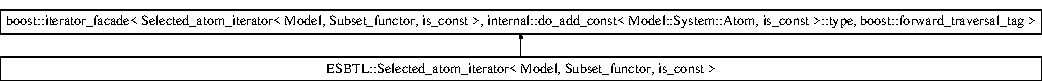
\includegraphics[height=1.084221cm]{classESBTL_1_1Selected__atom__iterator}
\end{center}
\end{figure}
\subsection*{Public Member Functions}
\begin{DoxyCompactItemize}
\item 
\hyperlink{classESBTL_1_1Selected__atom__iterator_a90cd448bdf3d57cd774c0bbcfbe402df}{Selected\+\_\+atom\+\_\+iterator} (Base\+\_\+iterator it, const Subset\+\_\+functor \&functor)
\item 
\hyperlink{classESBTL_1_1Selected__atom__iterator_aeabc4e8a95fca2d11566f7ad8caf31ed}{Selected\+\_\+atom\+\_\+iterator} (Base\+\_\+iterator it)
\end{DoxyCompactItemize}
\subsection*{Friends}
\begin{DoxyCompactItemize}
\item 
class \hyperlink{classESBTL_1_1Selected__atom__iterator_ac09f73e325921cc50ebcd96bed0f8096}{boost\+::iterator\+\_\+core\+\_\+access}
\end{DoxyCompactItemize}


\subsection{Detailed Description}
\subsubsection*{template$<$class Model, class Subset\+\_\+functor, bool is\+\_\+const$>$\newline
class E\+S\+B\+T\+L\+::\+Selected\+\_\+atom\+\_\+iterator$<$ Model, Subset\+\_\+functor, is\+\_\+const $>$}

Class defining an iterator over atoms of a model, restricted to a certain type defined by a function object. 
\begin{DoxyTemplParams}{Template Parameters}
{\em Model} & is the type of the model used. \\
\hline
{\em Subset\+\_\+functor} & is a function following the concept of \hyperlink{group__atomsel}{Atom selection}. \\
\hline
{\em is\+\_\+const} & indicates the constness of the iterator.\\
\hline
\end{DoxyTemplParams}
If you do not need to pass a state to your functor, you might want to use boost\+::filter\+\_\+iterator instead. 

\subsection{Constructor \& Destructor Documentation}
\mbox{\Hypertarget{classESBTL_1_1Selected__atom__iterator_a90cd448bdf3d57cd774c0bbcfbe402df}\label{classESBTL_1_1Selected__atom__iterator_a90cd448bdf3d57cd774c0bbcfbe402df}} 
\index{E\+S\+B\+T\+L\+::\+Selected\+\_\+atom\+\_\+iterator@{E\+S\+B\+T\+L\+::\+Selected\+\_\+atom\+\_\+iterator}!Selected\+\_\+atom\+\_\+iterator@{Selected\+\_\+atom\+\_\+iterator}}
\index{Selected\+\_\+atom\+\_\+iterator@{Selected\+\_\+atom\+\_\+iterator}!E\+S\+B\+T\+L\+::\+Selected\+\_\+atom\+\_\+iterator@{E\+S\+B\+T\+L\+::\+Selected\+\_\+atom\+\_\+iterator}}
\subsubsection{\texorpdfstring{Selected\+\_\+atom\+\_\+iterator()}{Selected\_atom\_iterator()}\hspace{0.1cm}{\footnotesize\ttfamily [1/2]}}
{\footnotesize\ttfamily template$<$class Model, class Subset\+\_\+functor, bool is\+\_\+const$>$ \\
\hyperlink{classESBTL_1_1Selected__atom__iterator}{E\+S\+B\+T\+L\+::\+Selected\+\_\+atom\+\_\+iterator}$<$ Model, Subset\+\_\+functor, is\+\_\+const $>$\+::\hyperlink{classESBTL_1_1Selected__atom__iterator}{Selected\+\_\+atom\+\_\+iterator} (\begin{DoxyParamCaption}\item[{Base\+\_\+iterator}]{it,  }\item[{const Subset\+\_\+functor \&}]{functor }\end{DoxyParamCaption})\hspace{0.3cm}{\ttfamily [inline]}}

Constructor. 
\begin{DoxyParams}{Parameters}
{\em it} & is the iterator indicating the starting point for the iterator. \\
\hline
{\em functor} & is the functor used to select atoms. \\
\hline
\end{DoxyParams}
\mbox{\Hypertarget{classESBTL_1_1Selected__atom__iterator_aeabc4e8a95fca2d11566f7ad8caf31ed}\label{classESBTL_1_1Selected__atom__iterator_aeabc4e8a95fca2d11566f7ad8caf31ed}} 
\index{E\+S\+B\+T\+L\+::\+Selected\+\_\+atom\+\_\+iterator@{E\+S\+B\+T\+L\+::\+Selected\+\_\+atom\+\_\+iterator}!Selected\+\_\+atom\+\_\+iterator@{Selected\+\_\+atom\+\_\+iterator}}
\index{Selected\+\_\+atom\+\_\+iterator@{Selected\+\_\+atom\+\_\+iterator}!E\+S\+B\+T\+L\+::\+Selected\+\_\+atom\+\_\+iterator@{E\+S\+B\+T\+L\+::\+Selected\+\_\+atom\+\_\+iterator}}
\subsubsection{\texorpdfstring{Selected\+\_\+atom\+\_\+iterator()}{Selected\_atom\_iterator()}\hspace{0.1cm}{\footnotesize\ttfamily [2/2]}}
{\footnotesize\ttfamily template$<$class Model, class Subset\+\_\+functor, bool is\+\_\+const$>$ \\
\hyperlink{classESBTL_1_1Selected__atom__iterator}{E\+S\+B\+T\+L\+::\+Selected\+\_\+atom\+\_\+iterator}$<$ Model, Subset\+\_\+functor, is\+\_\+const $>$\+::\hyperlink{classESBTL_1_1Selected__atom__iterator}{Selected\+\_\+atom\+\_\+iterator} (\begin{DoxyParamCaption}\item[{Base\+\_\+iterator}]{it }\end{DoxyParamCaption})\hspace{0.3cm}{\ttfamily [inline]}}



\subsection{Friends And Related Function Documentation}
\mbox{\Hypertarget{classESBTL_1_1Selected__atom__iterator_ac09f73e325921cc50ebcd96bed0f8096}\label{classESBTL_1_1Selected__atom__iterator_ac09f73e325921cc50ebcd96bed0f8096}} 
\index{E\+S\+B\+T\+L\+::\+Selected\+\_\+atom\+\_\+iterator@{E\+S\+B\+T\+L\+::\+Selected\+\_\+atom\+\_\+iterator}!boost\+::iterator\+\_\+core\+\_\+access@{boost\+::iterator\+\_\+core\+\_\+access}}
\index{boost\+::iterator\+\_\+core\+\_\+access@{boost\+::iterator\+\_\+core\+\_\+access}!E\+S\+B\+T\+L\+::\+Selected\+\_\+atom\+\_\+iterator@{E\+S\+B\+T\+L\+::\+Selected\+\_\+atom\+\_\+iterator}}
\subsubsection{\texorpdfstring{boost\+::iterator\+\_\+core\+\_\+access}{boost::iterator\_core\_access}}
{\footnotesize\ttfamily template$<$class Model, class Subset\+\_\+functor, bool is\+\_\+const$>$ \\
friend class boost\+::iterator\+\_\+core\+\_\+access\hspace{0.3cm}{\ttfamily [friend]}}



The documentation for this class was generated from the following file\+:\begin{DoxyCompactItemize}
\item 
\hyperlink{selected__atom__iterator_8h}{selected\+\_\+atom\+\_\+iterator.\+h}\end{DoxyCompactItemize}

\hypertarget{structESBTL_1_1System__items__with__coarse__grain}{}\section{E\+S\+B\+TL\+:\+:System\+\_\+items\+\_\+with\+\_\+coarse\+\_\+grain Struct Reference}
\label{structESBTL_1_1System__items__with__coarse__grain}\index{E\+S\+B\+T\+L\+::\+System\+\_\+items\+\_\+with\+\_\+coarse\+\_\+grain@{E\+S\+B\+T\+L\+::\+System\+\_\+items\+\_\+with\+\_\+coarse\+\_\+grain}}


{\ttfamily \#include $<$coarse\+\_\+grain.\+h$>$}

\subsection*{Classes}
\begin{DoxyCompactItemize}
\item 
struct \hyperlink{structESBTL_1_1System__items__with__coarse__grain_1_1Atom__wrapper}{Atom\+\_\+wrapper}
\item 
struct \hyperlink{structESBTL_1_1System__items__with__coarse__grain_1_1Chain__wrapper}{Chain\+\_\+wrapper}
\item 
struct \hyperlink{structESBTL_1_1System__items__with__coarse__grain_1_1Model__wrapper}{Model\+\_\+wrapper}
\item 
class \hyperlink{classESBTL_1_1System__items__with__coarse__grain_1_1Residue__wrapper}{Residue\+\_\+wrapper}
\end{DoxyCompactItemize}


\subsection{Detailed Description}
A default coarse-\/grain system items gathering wrappers (needed to break the cyclic dependency) that allow to define a model, chain, residue and atom type from the types \hyperlink{classESBTL_1_1Molecular__model}{Molecular\+\_\+model}, \hyperlink{classESBTL_1_1Molecular__chain}{Molecular\+\_\+chain}, \hyperlink{classESBTL_1_1Coarse__residue}{Coarse\+\_\+residue} and \hyperlink{classESBTL_1_1Molecular__atom}{Molecular\+\_\+atom} respectively. 

The documentation for this struct was generated from the following file\+:\begin{DoxyCompactItemize}
\item 
\hyperlink{coarse__grain_8h}{coarse\+\_\+grain.\+h}\end{DoxyCompactItemize}

\hypertarget{classESBTL_1_1System__updater__from__xdrfile}{}\section{E\+S\+B\+TL\+:\+:System\+\_\+updater\+\_\+from\+\_\+xdrfile$<$ System $>$ Class Template Reference}
\label{classESBTL_1_1System__updater__from__xdrfile}\index{E\+S\+B\+T\+L\+::\+System\+\_\+updater\+\_\+from\+\_\+xdrfile$<$ System $>$@{E\+S\+B\+T\+L\+::\+System\+\_\+updater\+\_\+from\+\_\+xdrfile$<$ System $>$}}


{\ttfamily \#include $<$system\+\_\+updater\+\_\+from\+\_\+xdrfile.\+h$>$}

\subsection*{Public Member Functions}
\begin{DoxyCompactItemize}
\item 
{\footnotesize template$<$class System\+\_\+iterator $>$ }\\\hyperlink{classESBTL_1_1System__updater__from__xdrfile_ab8ec6b14664c00a39bc8878c54514307}{System\+\_\+updater\+\_\+from\+\_\+xdrfile} (System\+\_\+iterator begin, System\+\_\+iterator end, unsigned model\+\_\+selected\+\_\+, const std\+::string \&xtc\+\_\+fname, unsigned max\+\_\+atoms, unsigned read\+\_\+from=1, unsigned read\+\_\+to=std\+::numeric\+\_\+limits$<$ unsigned $>$\+::max())
\item 
\hyperlink{classESBTL_1_1System__updater__from__xdrfile_a2023589e3370c4826ece05e8c197ae70}{$\sim$\+System\+\_\+updater\+\_\+from\+\_\+xdrfile} ()
\item 
boost\+::tuple$<$ bool, double, int $>$ \hyperlink{classESBTL_1_1System__updater__from__xdrfile_a295ff6221508724b6a7a6d2c95990195}{next\+\_\+frame} (bool is\+\_\+init=false)
\item 
bool \hyperlink{classESBTL_1_1System__updater__from__xdrfile_a9c7da450c1690fa709304039fe47f57b}{has\+\_\+more\+\_\+frames} ()
\item 
const unsigned \& \hyperlink{classESBTL_1_1System__updater__from__xdrfile_ab3c93e0cd396173a06668501f63f54a8}{current\+\_\+frame\+\_\+id} ()
\end{DoxyCompactItemize}


\subsection{Detailed Description}
\subsubsection*{template$<$class System$>$\newline
class E\+S\+B\+T\+L\+::\+System\+\_\+updater\+\_\+from\+\_\+xdrfile$<$ System $>$}

Helper class responsible for updating the coordinates of a system according to a trajectory read from an xtc file. The system must already have been constructed (from a \hyperlink{namespaceESBTL_1_1PDB}{P\+DB} file for example).

Note that using this class requires that the xdrfile library and header to be installed on your system (available as a package for your distribution or at \href{ftp://ftp.gromacs.org/pub/contrib/xdrfile-1.1.tar.gz}{\tt ftp\+://ftp.\+gromacs.\+org/pub/contrib/xdrfile-\/1.\+1.\+tar.\+gz}).

Refer to \href{http://www.gromacs.org}{\tt http\+://www.\+gromacs.\+org} for more information. 
\begin{DoxyTemplParams}{Template Parameters}
{\em System} & is the type of the system used. \\
\hline
\end{DoxyTemplParams}


\subsection{Constructor \& Destructor Documentation}
\mbox{\Hypertarget{classESBTL_1_1System__updater__from__xdrfile_ab8ec6b14664c00a39bc8878c54514307}\label{classESBTL_1_1System__updater__from__xdrfile_ab8ec6b14664c00a39bc8878c54514307}} 
\index{E\+S\+B\+T\+L\+::\+System\+\_\+updater\+\_\+from\+\_\+xdrfile@{E\+S\+B\+T\+L\+::\+System\+\_\+updater\+\_\+from\+\_\+xdrfile}!System\+\_\+updater\+\_\+from\+\_\+xdrfile@{System\+\_\+updater\+\_\+from\+\_\+xdrfile}}
\index{System\+\_\+updater\+\_\+from\+\_\+xdrfile@{System\+\_\+updater\+\_\+from\+\_\+xdrfile}!E\+S\+B\+T\+L\+::\+System\+\_\+updater\+\_\+from\+\_\+xdrfile@{E\+S\+B\+T\+L\+::\+System\+\_\+updater\+\_\+from\+\_\+xdrfile}}
\subsubsection{\texorpdfstring{System\+\_\+updater\+\_\+from\+\_\+xdrfile()}{System\_updater\_from\_xdrfile()}}
{\footnotesize\ttfamily template$<$class System $>$ \\
template$<$class System\+\_\+iterator $>$ \\
\hyperlink{classESBTL_1_1System__updater__from__xdrfile}{E\+S\+B\+T\+L\+::\+System\+\_\+updater\+\_\+from\+\_\+xdrfile}$<$ System $>$\+::\hyperlink{classESBTL_1_1System__updater__from__xdrfile}{System\+\_\+updater\+\_\+from\+\_\+xdrfile} (\begin{DoxyParamCaption}\item[{System\+\_\+iterator}]{begin,  }\item[{System\+\_\+iterator}]{end,  }\item[{unsigned}]{model\+\_\+selected\+\_\+,  }\item[{const std\+::string \&}]{xtc\+\_\+fname,  }\item[{unsigned}]{max\+\_\+atoms,  }\item[{unsigned}]{read\+\_\+from = {\ttfamily 1},  }\item[{unsigned}]{read\+\_\+to = {\ttfamily std\+:\+:numeric\+\_\+limits$<$unsigned$>$\+:\+:max()} }\end{DoxyParamCaption})\hspace{0.3cm}{\ttfamily [inline]}}

Constructor. It requires an already build model (from a \hyperlink{namespaceESBTL_1_1PDB}{P\+DB} file for example.) 
\begin{DoxyTemplParams}{Template Parameters}
{\em System\+\_\+iterator} & is an iterator over systems used. \\
\hline
\end{DoxyTemplParams}

\begin{DoxyParams}{Parameters}
{\em begin} & is an iterator over the first system that need to be updated. \\
\hline
{\em end} & is a past iterator over the last system that need to be updated. \\
\hline
{\em model\+\_\+selected\+\_\+} & indicates the number of the model to be updated. \\
\hline
{\em xtc\+\_\+fname} & is the path to the xtc file used to update the system coordinates. \\
\hline
{\em max\+\_\+atoms} & is an upper bound on the number of atoms contains in a frame. \\
\hline
{\em read\+\_\+from} & is the index of the first frame to be loaded. \\
\hline
{\em read\+\_\+to} & is the index of the last frame to be loaded. \\
\hline
\end{DoxyParams}
\mbox{\Hypertarget{classESBTL_1_1System__updater__from__xdrfile_a2023589e3370c4826ece05e8c197ae70}\label{classESBTL_1_1System__updater__from__xdrfile_a2023589e3370c4826ece05e8c197ae70}} 
\index{E\+S\+B\+T\+L\+::\+System\+\_\+updater\+\_\+from\+\_\+xdrfile@{E\+S\+B\+T\+L\+::\+System\+\_\+updater\+\_\+from\+\_\+xdrfile}!````~System\+\_\+updater\+\_\+from\+\_\+xdrfile@{$\sim$\+System\+\_\+updater\+\_\+from\+\_\+xdrfile}}
\index{````~System\+\_\+updater\+\_\+from\+\_\+xdrfile@{$\sim$\+System\+\_\+updater\+\_\+from\+\_\+xdrfile}!E\+S\+B\+T\+L\+::\+System\+\_\+updater\+\_\+from\+\_\+xdrfile@{E\+S\+B\+T\+L\+::\+System\+\_\+updater\+\_\+from\+\_\+xdrfile}}
\subsubsection{\texorpdfstring{$\sim$\+System\+\_\+updater\+\_\+from\+\_\+xdrfile()}{~System\_updater\_from\_xdrfile()}}
{\footnotesize\ttfamily template$<$class System $>$ \\
\hyperlink{classESBTL_1_1System__updater__from__xdrfile}{E\+S\+B\+T\+L\+::\+System\+\_\+updater\+\_\+from\+\_\+xdrfile}$<$ System $>$\+::$\sim$\hyperlink{classESBTL_1_1System__updater__from__xdrfile}{System\+\_\+updater\+\_\+from\+\_\+xdrfile} (\begin{DoxyParamCaption}{ }\end{DoxyParamCaption})\hspace{0.3cm}{\ttfamily [inline]}}



\subsection{Member Function Documentation}
\mbox{\Hypertarget{classESBTL_1_1System__updater__from__xdrfile_ab3c93e0cd396173a06668501f63f54a8}\label{classESBTL_1_1System__updater__from__xdrfile_ab3c93e0cd396173a06668501f63f54a8}} 
\index{E\+S\+B\+T\+L\+::\+System\+\_\+updater\+\_\+from\+\_\+xdrfile@{E\+S\+B\+T\+L\+::\+System\+\_\+updater\+\_\+from\+\_\+xdrfile}!current\+\_\+frame\+\_\+id@{current\+\_\+frame\+\_\+id}}
\index{current\+\_\+frame\+\_\+id@{current\+\_\+frame\+\_\+id}!E\+S\+B\+T\+L\+::\+System\+\_\+updater\+\_\+from\+\_\+xdrfile@{E\+S\+B\+T\+L\+::\+System\+\_\+updater\+\_\+from\+\_\+xdrfile}}
\subsubsection{\texorpdfstring{current\+\_\+frame\+\_\+id()}{current\_frame\_id()}}
{\footnotesize\ttfamily template$<$class System $>$ \\
const unsigned\& \hyperlink{classESBTL_1_1System__updater__from__xdrfile}{E\+S\+B\+T\+L\+::\+System\+\_\+updater\+\_\+from\+\_\+xdrfile}$<$ System $>$\+::current\+\_\+frame\+\_\+id (\begin{DoxyParamCaption}{ }\end{DoxyParamCaption})\hspace{0.3cm}{\ttfamily [inline]}}

\mbox{\Hypertarget{classESBTL_1_1System__updater__from__xdrfile_a9c7da450c1690fa709304039fe47f57b}\label{classESBTL_1_1System__updater__from__xdrfile_a9c7da450c1690fa709304039fe47f57b}} 
\index{E\+S\+B\+T\+L\+::\+System\+\_\+updater\+\_\+from\+\_\+xdrfile@{E\+S\+B\+T\+L\+::\+System\+\_\+updater\+\_\+from\+\_\+xdrfile}!has\+\_\+more\+\_\+frames@{has\+\_\+more\+\_\+frames}}
\index{has\+\_\+more\+\_\+frames@{has\+\_\+more\+\_\+frames}!E\+S\+B\+T\+L\+::\+System\+\_\+updater\+\_\+from\+\_\+xdrfile@{E\+S\+B\+T\+L\+::\+System\+\_\+updater\+\_\+from\+\_\+xdrfile}}
\subsubsection{\texorpdfstring{has\+\_\+more\+\_\+frames()}{has\_more\_frames()}}
{\footnotesize\ttfamily template$<$class System $>$ \\
bool \hyperlink{classESBTL_1_1System__updater__from__xdrfile}{E\+S\+B\+T\+L\+::\+System\+\_\+updater\+\_\+from\+\_\+xdrfile}$<$ System $>$\+::has\+\_\+more\+\_\+frames (\begin{DoxyParamCaption}{ }\end{DoxyParamCaption})\hspace{0.3cm}{\ttfamily [inline]}}

Indicates whether a frame is available to update the system. \mbox{\Hypertarget{classESBTL_1_1System__updater__from__xdrfile_a295ff6221508724b6a7a6d2c95990195}\label{classESBTL_1_1System__updater__from__xdrfile_a295ff6221508724b6a7a6d2c95990195}} 
\index{E\+S\+B\+T\+L\+::\+System\+\_\+updater\+\_\+from\+\_\+xdrfile@{E\+S\+B\+T\+L\+::\+System\+\_\+updater\+\_\+from\+\_\+xdrfile}!next\+\_\+frame@{next\+\_\+frame}}
\index{next\+\_\+frame@{next\+\_\+frame}!E\+S\+B\+T\+L\+::\+System\+\_\+updater\+\_\+from\+\_\+xdrfile@{E\+S\+B\+T\+L\+::\+System\+\_\+updater\+\_\+from\+\_\+xdrfile}}
\subsubsection{\texorpdfstring{next\+\_\+frame()}{next\_frame()}}
{\footnotesize\ttfamily template$<$class System $>$ \\
boost\+::tuple$<$bool,double,int$>$ \hyperlink{classESBTL_1_1System__updater__from__xdrfile}{E\+S\+B\+T\+L\+::\+System\+\_\+updater\+\_\+from\+\_\+xdrfile}$<$ System $>$\+::next\+\_\+frame (\begin{DoxyParamCaption}\item[{bool}]{is\+\_\+init = {\ttfamily false} }\end{DoxyParamCaption})\hspace{0.3cm}{\ttfamily [inline]}}

Loads the next frame into the system (update coordinates). \begin{DoxyReturn}{Returns}
the tuple returned contains a boolean (indicating whether the next frame could be loaded), a double (indicating the time of the frame in the simulation) and an integer (indicating the simulation step). 
\end{DoxyReturn}


The documentation for this class was generated from the following file\+:\begin{DoxyCompactItemize}
\item 
\hyperlink{system__updater__from__xdrfile_8h}{system\+\_\+updater\+\_\+from\+\_\+xdrfile.\+h}\end{DoxyCompactItemize}

\hypertarget{structESBTL_1_1Traits__for__grid}{}\section{E\+S\+B\+TL\+:\+:Traits\+\_\+for\+\_\+grid$<$ Point\+\_\+, Iterator\+\_\+ $>$ Struct Template Reference}
\label{structESBTL_1_1Traits__for__grid}\index{E\+S\+B\+T\+L\+::\+Traits\+\_\+for\+\_\+grid$<$ Point\+\_\+, Iterator\+\_\+ $>$@{E\+S\+B\+T\+L\+::\+Traits\+\_\+for\+\_\+grid$<$ Point\+\_\+, Iterator\+\_\+ $>$}}


{\ttfamily \#include $<$grid\+\_\+of\+\_\+cubes.\+h$>$}

\subsection*{Public Types}
\begin{DoxyCompactItemize}
\item 
typedef double \hyperlink{structESBTL_1_1Traits__for__grid_a2d1eddf80f02f912cd39b58c9356dd83}{NT}
\item 
typedef Iterator\+\_\+ \hyperlink{structESBTL_1_1Traits__for__grid_af8465e0f6ef165f72a3ca602e5b17445}{Iterator}
\item 
typedef Point\+\_\+ \hyperlink{structESBTL_1_1Traits__for__grid_a9e1fa4c89963d77117ce5eaead5ce7a1}{Point}
\end{DoxyCompactItemize}
\subsection*{Static Public Member Functions}
\begin{DoxyCompactItemize}
\item 
static void \hyperlink{structESBTL_1_1Traits__for__grid_a6456ed3dd1cba28aa5081f4fd2270880}{init\+\_\+grid} (const \hyperlink{structESBTL_1_1Traits__for__grid_af8465e0f6ef165f72a3ca602e5b17445}{Iterator} \&begin, const \hyperlink{structESBTL_1_1Traits__for__grid_af8465e0f6ef165f72a3ca602e5b17445}{Iterator} \&end, int \&xlim, int \&ylim, int \&zlim, double \&rmax, \hyperlink{structESBTL_1_1Traits__for__grid_a9e1fa4c89963d77117ce5eaead5ce7a1}{Point} \&lower\+\_\+corner)
\item 
{\footnotesize template$<$class Any\+\_\+iterator $>$ }\\static boost\+::tuple$<$ int, int, int $>$ \hyperlink{structESBTL_1_1Traits__for__grid_ace6769e2b498f72a9bd02df769299df2}{locate\+\_\+cube} (Any\+\_\+iterator it, const int \&xlim, const int \&ylim, const int \&zlim, const double \&cubel, const \hyperlink{structESBTL_1_1Traits__for__grid_a9e1fa4c89963d77117ce5eaead5ce7a1}{Point} \&lower\+\_\+corner)
\item 
{\footnotesize template$<$class Any\+\_\+iterator $>$ }\\static bool \hyperlink{structESBTL_1_1Traits__for__grid_ab937229626216c683d664c6441020185}{is\+\_\+outside\+\_\+grid} (Any\+\_\+iterator it, const int \&xlim, const int \&ylim, const int \&zlim, const double \&cubel, const \hyperlink{structESBTL_1_1Traits__for__grid_a9e1fa4c89963d77117ce5eaead5ce7a1}{Point} \&lower\+\_\+corner)
\end{DoxyCompactItemize}


\subsection{Detailed Description}
\subsubsection*{template$<$class Point\+\_\+, class Iterator\+\_\+$>$\newline
struct E\+S\+B\+T\+L\+::\+Traits\+\_\+for\+\_\+grid$<$ Point\+\_\+, Iterator\+\_\+ $>$}

Traits for using with \hyperlink{structESBTL_1_1Grid__of__cubes}{Grid\+\_\+of\+\_\+cubes}. Objects are atoms/points, maximum radius is fixed to 3. 
\begin{DoxyTemplParams}{Template Parameters}
{\em Point\+\_\+} & is the underlying point type used. \\
\hline
{\em Iterator\+\_\+} & is an iterator over objects to be stored in the grid. \\
\hline
\end{DoxyTemplParams}


\subsection{Member Typedef Documentation}
\mbox{\Hypertarget{structESBTL_1_1Traits__for__grid_af8465e0f6ef165f72a3ca602e5b17445}\label{structESBTL_1_1Traits__for__grid_af8465e0f6ef165f72a3ca602e5b17445}} 
\index{E\+S\+B\+T\+L\+::\+Traits\+\_\+for\+\_\+grid@{E\+S\+B\+T\+L\+::\+Traits\+\_\+for\+\_\+grid}!Iterator@{Iterator}}
\index{Iterator@{Iterator}!E\+S\+B\+T\+L\+::\+Traits\+\_\+for\+\_\+grid@{E\+S\+B\+T\+L\+::\+Traits\+\_\+for\+\_\+grid}}
\subsubsection{\texorpdfstring{Iterator}{Iterator}}
{\footnotesize\ttfamily template$<$class Point\+\_\+ , class Iterator\+\_\+ $>$ \\
typedef Iterator\+\_\+ \hyperlink{structESBTL_1_1Traits__for__grid}{E\+S\+B\+T\+L\+::\+Traits\+\_\+for\+\_\+grid}$<$ Point\+\_\+, Iterator\+\_\+ $>$\+::\hyperlink{structESBTL_1_1Traits__for__grid_af8465e0f6ef165f72a3ca602e5b17445}{Iterator}}

\mbox{\Hypertarget{structESBTL_1_1Traits__for__grid_a2d1eddf80f02f912cd39b58c9356dd83}\label{structESBTL_1_1Traits__for__grid_a2d1eddf80f02f912cd39b58c9356dd83}} 
\index{E\+S\+B\+T\+L\+::\+Traits\+\_\+for\+\_\+grid@{E\+S\+B\+T\+L\+::\+Traits\+\_\+for\+\_\+grid}!NT@{NT}}
\index{NT@{NT}!E\+S\+B\+T\+L\+::\+Traits\+\_\+for\+\_\+grid@{E\+S\+B\+T\+L\+::\+Traits\+\_\+for\+\_\+grid}}
\subsubsection{\texorpdfstring{NT}{NT}}
{\footnotesize\ttfamily template$<$class Point\+\_\+ , class Iterator\+\_\+ $>$ \\
typedef double \hyperlink{structESBTL_1_1Traits__for__grid}{E\+S\+B\+T\+L\+::\+Traits\+\_\+for\+\_\+grid}$<$ Point\+\_\+, Iterator\+\_\+ $>$\+::\hyperlink{structESBTL_1_1Traits__for__grid_a2d1eddf80f02f912cd39b58c9356dd83}{NT}}

\mbox{\Hypertarget{structESBTL_1_1Traits__for__grid_a9e1fa4c89963d77117ce5eaead5ce7a1}\label{structESBTL_1_1Traits__for__grid_a9e1fa4c89963d77117ce5eaead5ce7a1}} 
\index{E\+S\+B\+T\+L\+::\+Traits\+\_\+for\+\_\+grid@{E\+S\+B\+T\+L\+::\+Traits\+\_\+for\+\_\+grid}!Point@{Point}}
\index{Point@{Point}!E\+S\+B\+T\+L\+::\+Traits\+\_\+for\+\_\+grid@{E\+S\+B\+T\+L\+::\+Traits\+\_\+for\+\_\+grid}}
\subsubsection{\texorpdfstring{Point}{Point}}
{\footnotesize\ttfamily template$<$class Point\+\_\+ , class Iterator\+\_\+ $>$ \\
typedef Point\+\_\+ \hyperlink{structESBTL_1_1Traits__for__grid}{E\+S\+B\+T\+L\+::\+Traits\+\_\+for\+\_\+grid}$<$ Point\+\_\+, Iterator\+\_\+ $>$\+::\hyperlink{structESBTL_1_1Traits__for__grid_a9e1fa4c89963d77117ce5eaead5ce7a1}{Point}}



\subsection{Member Function Documentation}
\mbox{\Hypertarget{structESBTL_1_1Traits__for__grid_a6456ed3dd1cba28aa5081f4fd2270880}\label{structESBTL_1_1Traits__for__grid_a6456ed3dd1cba28aa5081f4fd2270880}} 
\index{E\+S\+B\+T\+L\+::\+Traits\+\_\+for\+\_\+grid@{E\+S\+B\+T\+L\+::\+Traits\+\_\+for\+\_\+grid}!init\+\_\+grid@{init\+\_\+grid}}
\index{init\+\_\+grid@{init\+\_\+grid}!E\+S\+B\+T\+L\+::\+Traits\+\_\+for\+\_\+grid@{E\+S\+B\+T\+L\+::\+Traits\+\_\+for\+\_\+grid}}
\subsubsection{\texorpdfstring{init\+\_\+grid()}{init\_grid()}}
{\footnotesize\ttfamily template$<$class Point\+\_\+ , class Iterator\+\_\+ $>$ \\
static void \hyperlink{structESBTL_1_1Traits__for__grid}{E\+S\+B\+T\+L\+::\+Traits\+\_\+for\+\_\+grid}$<$ Point\+\_\+, Iterator\+\_\+ $>$\+::init\+\_\+grid (\begin{DoxyParamCaption}\item[{const \hyperlink{structESBTL_1_1Traits__for__grid_af8465e0f6ef165f72a3ca602e5b17445}{Iterator} \&}]{begin,  }\item[{const \hyperlink{structESBTL_1_1Traits__for__grid_af8465e0f6ef165f72a3ca602e5b17445}{Iterator} \&}]{end,  }\item[{int \&}]{xlim,  }\item[{int \&}]{ylim,  }\item[{int \&}]{zlim,  }\item[{double \&}]{rmax,  }\item[{\hyperlink{structESBTL_1_1Traits__for__grid_a9e1fa4c89963d77117ce5eaead5ce7a1}{Point} \&}]{lower\+\_\+corner }\end{DoxyParamCaption})\hspace{0.3cm}{\ttfamily [inline]}, {\ttfamily [static]}}

static function indicating how the grid must be initialized (the bounding box) 
\begin{DoxyParams}{Parameters}
{\em begin} & first iterator over the range of objects to be inserted into the grid. \\
\hline
{\em end} & past-\/end iterator over the range of objects to be inserted into the grid. \\
\hline
{\em xlim} & is the number of cubes in the x-\/direction. This value will be defined by that function. \\
\hline
{\em ylim} & is the number of cubes in the y-\/direction. This value will be defined by that function. \\
\hline
{\em zlim} & is the number of cubes in the z-\/direction. This value will be defined by that function. \\
\hline
{\em rmax} & is an upper bound on the radius of the atoms. This value will be defined by that function. \\
\hline
{\em lower\+\_\+corner} & is a point indicating the lower corner of the grid. This value will be defined by that function. \\
\hline
\end{DoxyParams}
\mbox{\Hypertarget{structESBTL_1_1Traits__for__grid_ab937229626216c683d664c6441020185}\label{structESBTL_1_1Traits__for__grid_ab937229626216c683d664c6441020185}} 
\index{E\+S\+B\+T\+L\+::\+Traits\+\_\+for\+\_\+grid@{E\+S\+B\+T\+L\+::\+Traits\+\_\+for\+\_\+grid}!is\+\_\+outside\+\_\+grid@{is\+\_\+outside\+\_\+grid}}
\index{is\+\_\+outside\+\_\+grid@{is\+\_\+outside\+\_\+grid}!E\+S\+B\+T\+L\+::\+Traits\+\_\+for\+\_\+grid@{E\+S\+B\+T\+L\+::\+Traits\+\_\+for\+\_\+grid}}
\subsubsection{\texorpdfstring{is\+\_\+outside\+\_\+grid()}{is\_outside\_grid()}}
{\footnotesize\ttfamily template$<$class Point\+\_\+ , class Iterator\+\_\+ $>$ \\
template$<$class Any\+\_\+iterator $>$ \\
static bool \hyperlink{structESBTL_1_1Traits__for__grid}{E\+S\+B\+T\+L\+::\+Traits\+\_\+for\+\_\+grid}$<$ Point\+\_\+, Iterator\+\_\+ $>$\+::is\+\_\+outside\+\_\+grid (\begin{DoxyParamCaption}\item[{Any\+\_\+iterator}]{it,  }\item[{const int \&}]{xlim,  }\item[{const int \&}]{ylim,  }\item[{const int \&}]{zlim,  }\item[{const double \&}]{cubel,  }\item[{const \hyperlink{structESBTL_1_1Traits__for__grid_a9e1fa4c89963d77117ce5eaead5ce7a1}{Point} \&}]{lower\+\_\+corner }\end{DoxyParamCaption})\hspace{0.3cm}{\ttfamily [inline]}, {\ttfamily [static]}}

static function indicating if an object can be in conflict with a grid object. 
\begin{DoxyParams}{Parameters}
{\em it} & is an iterator over an object. \\
\hline
{\em xlim} & is the number of cubes in the x-\/direction. \\
\hline
{\em ylim} & is the number of cubes in the y-\/direction. \\
\hline
{\em zlim} & is the number of cubes in the z-\/direction. \\
\hline
{\em cubel} & is the edge length of a cube in the grid. \\
\hline
{\em lower\+\_\+corner} & is a point indicating the lower corner of the grid. \\
\hline
\end{DoxyParams}
\begin{DoxyReturn}{Returns}
a tuple giving the cube position of the object in the grid. 
\end{DoxyReturn}
\mbox{\Hypertarget{structESBTL_1_1Traits__for__grid_ace6769e2b498f72a9bd02df769299df2}\label{structESBTL_1_1Traits__for__grid_ace6769e2b498f72a9bd02df769299df2}} 
\index{E\+S\+B\+T\+L\+::\+Traits\+\_\+for\+\_\+grid@{E\+S\+B\+T\+L\+::\+Traits\+\_\+for\+\_\+grid}!locate\+\_\+cube@{locate\+\_\+cube}}
\index{locate\+\_\+cube@{locate\+\_\+cube}!E\+S\+B\+T\+L\+::\+Traits\+\_\+for\+\_\+grid@{E\+S\+B\+T\+L\+::\+Traits\+\_\+for\+\_\+grid}}
\subsubsection{\texorpdfstring{locate\+\_\+cube()}{locate\_cube()}}
{\footnotesize\ttfamily template$<$class Point\+\_\+ , class Iterator\+\_\+ $>$ \\
template$<$class Any\+\_\+iterator $>$ \\
static boost\+::tuple$<$int,int,int$>$ \hyperlink{structESBTL_1_1Traits__for__grid}{E\+S\+B\+T\+L\+::\+Traits\+\_\+for\+\_\+grid}$<$ Point\+\_\+, Iterator\+\_\+ $>$\+::locate\+\_\+cube (\begin{DoxyParamCaption}\item[{Any\+\_\+iterator}]{it,  }\item[{const int \&}]{xlim,  }\item[{const int \&}]{ylim,  }\item[{const int \&}]{zlim,  }\item[{const double \&}]{cubel,  }\item[{const \hyperlink{structESBTL_1_1Traits__for__grid_a9e1fa4c89963d77117ce5eaead5ce7a1}{Point} \&}]{lower\+\_\+corner }\end{DoxyParamCaption})\hspace{0.3cm}{\ttfamily [inline]}, {\ttfamily [static]}}

static function computing the position of an object inside the grid. 
\begin{DoxyTemplParams}{Template Parameters}
{\em Any\+\_\+iterator} & is an iterator type over object to be stored in the grid. \\
\hline
\end{DoxyTemplParams}

\begin{DoxyParams}{Parameters}
{\em it} & is an iterator over an object. \\
\hline
{\em xlim} & is the number of cubes in the x-\/direction. \\
\hline
{\em ylim} & is the number of cubes in the y-\/direction. \\
\hline
{\em zlim} & is the number of cubes in the z-\/direction. \\
\hline
{\em cubel} & is the edge length of a cube in the grid. \\
\hline
{\em lower\+\_\+corner} & is a point indicating the lower corner of the grid. \\
\hline
\end{DoxyParams}
\begin{DoxyReturn}{Returns}
a tuple giving the cube position of the object in the grid. 
\end{DoxyReturn}


The documentation for this struct was generated from the following file\+:\begin{DoxyCompactItemize}
\item 
\hyperlink{grid__of__cubes_8h}{grid\+\_\+of\+\_\+cubes.\+h}\end{DoxyCompactItemize}

\hypertarget{structESBTL_1_1Weight__of__atoms}{}\section{E\+S\+B\+TL\+:\+:Weight\+\_\+of\+\_\+atoms$<$ Atom\+\_\+classifier $>$ Struct Template Reference}
\label{structESBTL_1_1Weight__of__atoms}\index{E\+S\+B\+T\+L\+::\+Weight\+\_\+of\+\_\+atoms$<$ Atom\+\_\+classifier $>$@{E\+S\+B\+T\+L\+::\+Weight\+\_\+of\+\_\+atoms$<$ Atom\+\_\+classifier $>$}}


{\ttfamily \#include $<$atom\+\_\+classifier.\+h$>$}

\subsection*{Public Member Functions}
\begin{DoxyCompactItemize}
\item 
\hyperlink{structESBTL_1_1Weight__of__atoms_a2225642c3cf2657680ac3ff82baf9e19}{Weight\+\_\+of\+\_\+atoms} (const Atom\+\_\+classifier $\ast$atom\+\_\+classifier)
\item 
Atom\+\_\+classifier\+::\+Properties\+::\+Value\+\_\+type \hyperlink{structESBTL_1_1Weight__of__atoms_adb65094d02fcf53a86e272c34ded0643}{operator()} (const typename Atom\+\_\+classifier\+::\+Query\+\_\+type \&atom) const
\end{DoxyCompactItemize}


\subsection{Detailed Description}
\subsubsection*{template$<$class Atom\+\_\+classifier$>$\newline
struct E\+S\+B\+T\+L\+::\+Weight\+\_\+of\+\_\+atoms$<$ Atom\+\_\+classifier $>$}

Function object providing the squared radius of an atom thanks to a classifier. 
\begin{DoxyTemplParams}{Template Parameters}
{\em Atom\+\_\+classifier} & is a classifier associating a radius to an atom. \\
\hline
\end{DoxyTemplParams}


\subsection{Constructor \& Destructor Documentation}
\mbox{\Hypertarget{structESBTL_1_1Weight__of__atoms_a2225642c3cf2657680ac3ff82baf9e19}\label{structESBTL_1_1Weight__of__atoms_a2225642c3cf2657680ac3ff82baf9e19}} 
\index{E\+S\+B\+T\+L\+::\+Weight\+\_\+of\+\_\+atoms@{E\+S\+B\+T\+L\+::\+Weight\+\_\+of\+\_\+atoms}!Weight\+\_\+of\+\_\+atoms@{Weight\+\_\+of\+\_\+atoms}}
\index{Weight\+\_\+of\+\_\+atoms@{Weight\+\_\+of\+\_\+atoms}!E\+S\+B\+T\+L\+::\+Weight\+\_\+of\+\_\+atoms@{E\+S\+B\+T\+L\+::\+Weight\+\_\+of\+\_\+atoms}}
\subsubsection{\texorpdfstring{Weight\+\_\+of\+\_\+atoms()}{Weight\_of\_atoms()}}
{\footnotesize\ttfamily template$<$class Atom\+\_\+classifier $>$ \\
\hyperlink{structESBTL_1_1Weight__of__atoms}{E\+S\+B\+T\+L\+::\+Weight\+\_\+of\+\_\+atoms}$<$ Atom\+\_\+classifier $>$\+::\hyperlink{structESBTL_1_1Weight__of__atoms}{Weight\+\_\+of\+\_\+atoms} (\begin{DoxyParamCaption}\item[{const Atom\+\_\+classifier $\ast$}]{atom\+\_\+classifier }\end{DoxyParamCaption})\hspace{0.3cm}{\ttfamily [inline]}}

Constructor 

\subsection{Member Function Documentation}
\mbox{\Hypertarget{structESBTL_1_1Weight__of__atoms_adb65094d02fcf53a86e272c34ded0643}\label{structESBTL_1_1Weight__of__atoms_adb65094d02fcf53a86e272c34ded0643}} 
\index{E\+S\+B\+T\+L\+::\+Weight\+\_\+of\+\_\+atoms@{E\+S\+B\+T\+L\+::\+Weight\+\_\+of\+\_\+atoms}!operator()@{operator()}}
\index{operator()@{operator()}!E\+S\+B\+T\+L\+::\+Weight\+\_\+of\+\_\+atoms@{E\+S\+B\+T\+L\+::\+Weight\+\_\+of\+\_\+atoms}}
\subsubsection{\texorpdfstring{operator()()}{operator()()}}
{\footnotesize\ttfamily template$<$class Atom\+\_\+classifier $>$ \\
Atom\+\_\+classifier\+::\+Properties\+::\+Value\+\_\+type \hyperlink{structESBTL_1_1Weight__of__atoms}{E\+S\+B\+T\+L\+::\+Weight\+\_\+of\+\_\+atoms}$<$ Atom\+\_\+classifier $>$\+::operator() (\begin{DoxyParamCaption}\item[{const typename Atom\+\_\+classifier\+::\+Query\+\_\+type \&}]{atom }\end{DoxyParamCaption}) const\hspace{0.3cm}{\ttfamily [inline]}}

Returns the squared radius of atom. 
\begin{DoxyParams}{Parameters}
{\em atom} & the atom used as query. \\
\hline
\end{DoxyParams}


The documentation for this struct was generated from the following file\+:\begin{DoxyCompactItemize}
\item 
\hyperlink{atom__classifier_8h}{atom\+\_\+classifier.\+h}\end{DoxyCompactItemize}

\hypertarget{classESBTL_1_1Weighted__atom__iterator}{}\section{E\+S\+B\+TL\+:\+:Weighted\+\_\+atom\+\_\+iterator$<$ Model, Weighted\+\_\+atom, Weight\+\_\+functor $>$ Class Template Reference}
\label{classESBTL_1_1Weighted__atom__iterator}\index{E\+S\+B\+T\+L\+::\+Weighted\+\_\+atom\+\_\+iterator$<$ Model, Weighted\+\_\+atom, Weight\+\_\+functor $>$@{E\+S\+B\+T\+L\+::\+Weighted\+\_\+atom\+\_\+iterator$<$ Model, Weighted\+\_\+atom, Weight\+\_\+functor $>$}}


{\ttfamily \#include $<$weighted\+\_\+atom\+\_\+iterator.\+h$>$}

Inheritance diagram for E\+S\+B\+TL\+:\+:Weighted\+\_\+atom\+\_\+iterator$<$ Model, Weighted\+\_\+atom, Weight\+\_\+functor $>$\+:\begin{figure}[H]
\begin{center}
\leavevmode
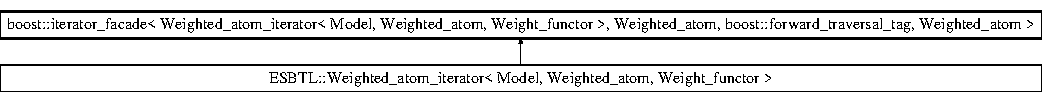
\includegraphics[height=1.240310cm]{classESBTL_1_1Weighted__atom__iterator}
\end{center}
\end{figure}
\subsection*{Public Member Functions}
\begin{DoxyCompactItemize}
\item 
{\footnotesize template$<$class Functor\+\_\+parameters $>$ }\\\hyperlink{classESBTL_1_1Weighted__atom__iterator_a41781a4ac59637e0d6577fe7b929fb99}{Weighted\+\_\+atom\+\_\+iterator} (typename Model\+::\+Atoms\+\_\+const\+\_\+iterator it, Functor\+\_\+parameters params)
\end{DoxyCompactItemize}
\subsection*{Friends}
\begin{DoxyCompactItemize}
\item 
class \hyperlink{classESBTL_1_1Weighted__atom__iterator_ac09f73e325921cc50ebcd96bed0f8096}{boost\+::iterator\+\_\+core\+\_\+access}
\end{DoxyCompactItemize}


\subsection{Detailed Description}
\subsubsection*{template$<$class Model, class Weighted\+\_\+atom, class Weight\+\_\+functor$>$\newline
class E\+S\+B\+T\+L\+::\+Weighted\+\_\+atom\+\_\+iterator$<$ Model, Weighted\+\_\+atom, Weight\+\_\+functor $>$}

Class providing an iterator over atoms of a model that returns a weighted point when dereferencing. This is particularly useful when using \hyperlink{namespaceESBTL_1_1CGAL}{C\+G\+AL} and its algorithms working on weighted points. 
\begin{DoxyTemplParams}{Template Parameters}
{\em Model} & is the type of model used. \\
\hline
{\em Weighted\+\_\+atom} & is the weighted point type returned. \\
\hline
{\em Weight\+\_\+functor} & is a function object which operator() associate a radius to an atom (as \hyperlink{structESBTL_1_1Weight__of__atoms}{Weight\+\_\+of\+\_\+atoms} for example.)\\
\hline
\end{DoxyTemplParams}
An alternative to this class is to use the class boost\+::transform\+\_\+iterator, provided your function object does not need only information available at compile time. 

\subsection{Constructor \& Destructor Documentation}
\mbox{\Hypertarget{classESBTL_1_1Weighted__atom__iterator_a41781a4ac59637e0d6577fe7b929fb99}\label{classESBTL_1_1Weighted__atom__iterator_a41781a4ac59637e0d6577fe7b929fb99}} 
\index{E\+S\+B\+T\+L\+::\+Weighted\+\_\+atom\+\_\+iterator@{E\+S\+B\+T\+L\+::\+Weighted\+\_\+atom\+\_\+iterator}!Weighted\+\_\+atom\+\_\+iterator@{Weighted\+\_\+atom\+\_\+iterator}}
\index{Weighted\+\_\+atom\+\_\+iterator@{Weighted\+\_\+atom\+\_\+iterator}!E\+S\+B\+T\+L\+::\+Weighted\+\_\+atom\+\_\+iterator@{E\+S\+B\+T\+L\+::\+Weighted\+\_\+atom\+\_\+iterator}}
\subsubsection{\texorpdfstring{Weighted\+\_\+atom\+\_\+iterator()}{Weighted\_atom\_iterator()}}
{\footnotesize\ttfamily template$<$class Model , class Weighted\+\_\+atom , class Weight\+\_\+functor $>$ \\
template$<$class Functor\+\_\+parameters $>$ \\
\hyperlink{classESBTL_1_1Weighted__atom__iterator}{E\+S\+B\+T\+L\+::\+Weighted\+\_\+atom\+\_\+iterator}$<$ Model, Weighted\+\_\+atom, Weight\+\_\+functor $>$\+::\hyperlink{classESBTL_1_1Weighted__atom__iterator}{Weighted\+\_\+atom\+\_\+iterator} (\begin{DoxyParamCaption}\item[{typename Model\+::\+Atoms\+\_\+const\+\_\+iterator}]{it,  }\item[{Functor\+\_\+parameters}]{params }\end{DoxyParamCaption})\hspace{0.3cm}{\ttfamily [inline]}}

Constructor. 
\begin{DoxyTemplParams}{Template Parameters}
{\em Functor\+\_\+parameters} & is a parameter type for the function object constructor. \\
\hline
\end{DoxyTemplParams}

\begin{DoxyParams}{Parameters}
{\em it} & is the corresponding atom iterator. \\
\hline
{\em params} & is a parameter given to the function object constructor. \\
\hline
\end{DoxyParams}


\subsection{Friends And Related Function Documentation}
\mbox{\Hypertarget{classESBTL_1_1Weighted__atom__iterator_ac09f73e325921cc50ebcd96bed0f8096}\label{classESBTL_1_1Weighted__atom__iterator_ac09f73e325921cc50ebcd96bed0f8096}} 
\index{E\+S\+B\+T\+L\+::\+Weighted\+\_\+atom\+\_\+iterator@{E\+S\+B\+T\+L\+::\+Weighted\+\_\+atom\+\_\+iterator}!boost\+::iterator\+\_\+core\+\_\+access@{boost\+::iterator\+\_\+core\+\_\+access}}
\index{boost\+::iterator\+\_\+core\+\_\+access@{boost\+::iterator\+\_\+core\+\_\+access}!E\+S\+B\+T\+L\+::\+Weighted\+\_\+atom\+\_\+iterator@{E\+S\+B\+T\+L\+::\+Weighted\+\_\+atom\+\_\+iterator}}
\subsubsection{\texorpdfstring{boost\+::iterator\+\_\+core\+\_\+access}{boost::iterator\_core\_access}}
{\footnotesize\ttfamily template$<$class Model , class Weighted\+\_\+atom , class Weight\+\_\+functor $>$ \\
friend class boost\+::iterator\+\_\+core\+\_\+access\hspace{0.3cm}{\ttfamily [friend]}}



The documentation for this class was generated from the following file\+:\begin{DoxyCompactItemize}
\item 
\hyperlink{weighted__atom__iterator_8h}{weighted\+\_\+atom\+\_\+iterator.\+h}\end{DoxyCompactItemize}

\chapter{File Documentation}
\hypertarget{atom__classifier_8h}{}\section{atom\+\_\+classifier.\+h File Reference}
\label{atom__classifier_8h}\index{atom\+\_\+classifier.\+h@{atom\+\_\+classifier.\+h}}
{\ttfamily \#include $<$boost/unordered\+\_\+map.\+hpp$>$}\newline
{\ttfamily \#include $<$boost/lexical\+\_\+cast.\+hpp$>$}\newline
{\ttfamily \#include $<$boost/algorithm/string.\+hpp$>$}\newline
{\ttfamily \#include $<$iostream$>$}\newline
{\ttfamily \#include $<$sstream$>$}\newline
{\ttfamily \#include $<$fstream$>$}\newline
\subsection*{Classes}
\begin{DoxyCompactItemize}
\item 
class \hyperlink{classESBTL_1_1Radius__of__atom}{E\+S\+B\+T\+L\+::\+Radius\+\_\+of\+\_\+atom$<$ N\+T, Atom $>$}
\item 
class \hyperlink{classESBTL_1_1Name__and__radius__of__atom}{E\+S\+B\+T\+L\+::\+Name\+\_\+and\+\_\+radius\+\_\+of\+\_\+atom$<$ N\+T, Atom $>$}
\item 
class \hyperlink{classESBTL_1_1Name__of__pair}{E\+S\+B\+T\+L\+::\+Name\+\_\+of\+\_\+pair}
\item 
struct \hyperlink{structESBTL_1_1Generic__classifier}{E\+S\+B\+T\+L\+::\+Generic\+\_\+classifier$<$ Properties\+\_\+ $>$}
\item 
struct \hyperlink{structESBTL_1_1Weight__of__atoms}{E\+S\+B\+T\+L\+::\+Weight\+\_\+of\+\_\+atoms$<$ Atom\+\_\+classifier $>$}
\end{DoxyCompactItemize}
\subsection*{Namespaces}
\begin{DoxyCompactItemize}
\item 
 \hyperlink{namespaceESBTL}{E\+S\+B\+TL}
\end{DoxyCompactItemize}
\subsection*{Functions}
\begin{DoxyCompactItemize}
\item 
{\footnotesize template$<$class NT , class Atom $>$ }\\NT \hyperlink{namespaceESBTL_a339234ee84fc86156f2d2971dd1fd027}{E\+S\+B\+T\+L\+::get\+\_\+radius} (const Radius\+\_\+of\+\_\+atom$<$ NT, Atom $>$ \&property)
\end{DoxyCompactItemize}

\hypertarget{atom__selectors_8h}{}\section{atom\+\_\+selectors.\+h File Reference}
\label{atom__selectors_8h}\index{atom\+\_\+selectors.\+h@{atom\+\_\+selectors.\+h}}
{\ttfamily \#include $<$set$>$}\newline
\subsection*{Classes}
\begin{DoxyCompactItemize}
\item 
struct \hyperlink{structESBTL_1_1Select__by__resname}{E\+S\+B\+T\+L\+::\+Select\+\_\+by\+\_\+resname}
\item 
struct \hyperlink{structESBTL_1_1Select__by__atmname}{E\+S\+B\+T\+L\+::\+Select\+\_\+by\+\_\+atmname}
\item 
struct \hyperlink{structESBTL_1_1Select__by__element}{E\+S\+B\+T\+L\+::\+Select\+\_\+by\+\_\+element}
\item 
class \hyperlink{classESBTL_1_1Select__by__chainids}{E\+S\+B\+T\+L\+::\+Select\+\_\+by\+\_\+chainids}
\end{DoxyCompactItemize}
\subsection*{Namespaces}
\begin{DoxyCompactItemize}
\item 
 \hyperlink{namespaceESBTL}{E\+S\+B\+TL}
\end{DoxyCompactItemize}

\hypertarget{builder_8h}{}\section{builder.\+h File Reference}
\label{builder_8h}\index{builder.\+h@{builder.\+h}}
{\ttfamily \#include $<$iostream$>$}\newline
\subsection*{Classes}
\begin{DoxyCompactItemize}
\item 
class \hyperlink{classESBTL_1_1All__atom__system__builder}{E\+S\+B\+T\+L\+::\+All\+\_\+atom\+\_\+system\+\_\+builder$<$ System $>$}
\end{DoxyCompactItemize}
\subsection*{Namespaces}
\begin{DoxyCompactItemize}
\item 
 \hyperlink{namespaceESBTL}{E\+S\+B\+TL}
\end{DoxyCompactItemize}

\hypertarget{EPIC__kernel__with__atom_8h}{}\section{C\+G\+A\+L/\+E\+P\+I\+C\+\_\+kernel\+\_\+with\+\_\+atom.h File Reference}
\label{EPIC__kernel__with__atom_8h}\index{C\+G\+A\+L/\+E\+P\+I\+C\+\_\+kernel\+\_\+with\+\_\+atom.\+h@{C\+G\+A\+L/\+E\+P\+I\+C\+\_\+kernel\+\_\+with\+\_\+atom.\+h}}
{\ttfamily \#include $<$E\+S\+B\+T\+L/constants.\+h$>$}\newline
{\ttfamily \#include $<$E\+S\+B\+T\+L/xyz\+\_\+utils.\+h$>$}\newline
{\ttfamily \#include $<$E\+S\+B\+T\+L/line\+\_\+selectors.\+h$>$}\newline
{\ttfamily \#include $<$E\+S\+B\+T\+L/builder.\+h$>$}\newline
{\ttfamily \#include $<$E\+S\+B\+T\+L/line\+\_\+reader.\+h$>$}\newline
{\ttfamily \#include $<$E\+S\+B\+T\+L/\+P\+D\+B.\+h$>$}\newline
{\ttfamily \#include $<$E\+S\+B\+T\+L/occupancy\+\_\+handlers.\+h$>$}\newline
{\ttfamily \#include $<$E\+S\+B\+T\+L/molecular\+\_\+system.\+h$>$}\newline
{\ttfamily \#include $<$E\+S\+B\+T\+L/coarse\+\_\+grain.\+h$>$}\newline
{\ttfamily \#include $<$C\+G\+A\+L/\+Cartesian.\+h$>$}\newline
{\ttfamily \#include $<$C\+G\+A\+L/\+Filtered\+\_\+kernel.\+h$>$}\newline
\subsection*{Classes}
\begin{DoxyCompactItemize}
\item 
class \hyperlink{classESBTL_1_1CGAL_1_1Cartesian__kernel__base}{E\+S\+B\+T\+L\+::\+C\+G\+A\+L\+::\+Cartesian\+\_\+kernel\+\_\+base$<$ K\+\_\+, K\+\_\+\+Base $>$}
\item 
struct \hyperlink{structESBTL_1_1CGAL_1_1Cartesian__kernel__base_1_1Base}{E\+S\+B\+T\+L\+::\+C\+G\+A\+L\+::\+Cartesian\+\_\+kernel\+\_\+base$<$ K\+\_\+, K\+\_\+\+Base $>$\+::\+Base$<$ Kernel2 $>$}
\item 
struct \hyperlink{structESBTL_1_1CGAL_1_1Kernel__with__atom}{E\+S\+B\+T\+L\+::\+C\+G\+A\+L\+::\+Kernel\+\_\+with\+\_\+atom$<$ F\+T\+\_\+ $>$}
\item 
class \hyperlink{classESBTL_1_1CGAL_1_1Cartesian__kernel__base__cg}{E\+S\+B\+T\+L\+::\+C\+G\+A\+L\+::\+Cartesian\+\_\+kernel\+\_\+base\+\_\+cg$<$ K\+\_\+, K\+\_\+\+Base $>$}
\item 
struct \hyperlink{structESBTL_1_1CGAL_1_1Cartesian__kernel__base__cg_1_1Base}{E\+S\+B\+T\+L\+::\+C\+G\+A\+L\+::\+Cartesian\+\_\+kernel\+\_\+base\+\_\+cg$<$ K\+\_\+, K\+\_\+\+Base $>$\+::\+Base$<$ Kernel2 $>$}
\item 
struct \hyperlink{structESBTL_1_1CGAL_1_1Kernel__with__coarse__atom}{E\+S\+B\+T\+L\+::\+C\+G\+A\+L\+::\+Kernel\+\_\+with\+\_\+coarse\+\_\+atom$<$ F\+T\+\_\+ $>$}
\end{DoxyCompactItemize}
\subsection*{Namespaces}
\begin{DoxyCompactItemize}
\item 
 \hyperlink{namespaceESBTL}{E\+S\+B\+TL}
\item 
 \hyperlink{namespaceESBTL_1_1CGAL}{E\+S\+B\+T\+L\+::\+C\+G\+AL}
\end{DoxyCompactItemize}
\subsection*{Typedefs}
\begin{DoxyCompactItemize}
\item 
typedef Molecular\+\_\+system$<$ Default\+\_\+system\+\_\+items, \+::C\+G\+A\+L\+::\+Simple\+\_\+cartesian$<$ double $>$\+::Point\+\_\+3 $>$ \hyperlink{namespaceESBTL_1_1CGAL_a0d1fd18cc9360ce0ba0cc2ea2ed8be68}{E\+S\+B\+T\+L\+::\+C\+G\+A\+L\+::\+Default\+\_\+system}
\item 
typedef \+::C\+G\+A\+L\+::\+Filtered\+\_\+kernel$<$ Kernel\+\_\+with\+\_\+atom$<$ double $>$ $>$ \hyperlink{namespaceESBTL_1_1CGAL_ac13df3c9add4e34942e608f17fb6971c}{E\+S\+B\+T\+L\+::\+C\+G\+A\+L\+::\+E\+P\+I\+C\+\_\+kernel\+\_\+with\+\_\+atom}
\item 
typedef Molecular\+\_\+system$<$ System\+\_\+items\+\_\+with\+\_\+coarse\+\_\+grain, \+::C\+G\+A\+L\+::\+Simple\+\_\+cartesian$<$ double $>$\+::Point\+\_\+3 $>$ \hyperlink{namespaceESBTL_1_1CGAL_a3c029e52b1d0fd721493a259336696db}{E\+S\+B\+T\+L\+::\+C\+G\+A\+L\+::\+System\+\_\+with\+\_\+coarse\+\_\+grain}
\item 
typedef \+::C\+G\+A\+L\+::\+Filtered\+\_\+kernel$<$ Kernel\+\_\+with\+\_\+coarse\+\_\+atom$<$ double $>$ $>$ \hyperlink{namespaceESBTL_1_1CGAL_a3e9468c7a5fd8e3d29abdfaa53ecd55d}{E\+S\+B\+T\+L\+::\+C\+G\+A\+L\+::\+E\+P\+I\+C\+\_\+kernel\+\_\+with\+\_\+coarse\+\_\+atom}
\end{DoxyCompactItemize}

\hypertarget{coarse__classifier_8h}{}\section{coarse\+\_\+classifier.\+h File Reference}
\label{coarse__classifier_8h}\index{coarse\+\_\+classifier.\+h@{coarse\+\_\+classifier.\+h}}
{\ttfamily \#include $<$E\+S\+B\+T\+L/atom\+\_\+classifier.\+h$>$}\newline
\subsection*{Classes}
\begin{DoxyCompactItemize}
\item 
class \hyperlink{classESBTL_1_1Radius__of__coarse__atom}{E\+S\+B\+T\+L\+::\+Radius\+\_\+of\+\_\+coarse\+\_\+atom$<$ N\+T, Coarse\+\_\+atom $>$}
\item 
struct \hyperlink{structESBTL_1_1Color__of__atom}{E\+S\+B\+T\+L\+::\+Color\+\_\+of\+\_\+atom$<$ Atom $>$}
\item 
class \hyperlink{classESBTL_1_1Color__of__residues}{E\+S\+B\+T\+L\+::\+Color\+\_\+of\+\_\+residues$<$ Atom $>$}
\end{DoxyCompactItemize}
\subsection*{Namespaces}
\begin{DoxyCompactItemize}
\item 
 \hyperlink{namespaceESBTL}{E\+S\+B\+TL}
\end{DoxyCompactItemize}
\subsection*{Functions}
\begin{DoxyCompactItemize}
\item 
{\footnotesize template$<$class NT , class Coarse\+\_\+atom $>$ }\\NT \hyperlink{namespaceESBTL_ab5f456cde3cd8e7210ac2d21366d52c9}{E\+S\+B\+T\+L\+::get\+\_\+radius} (const Radius\+\_\+of\+\_\+coarse\+\_\+atom$<$ NT, Coarse\+\_\+atom $>$ \&property)
\end{DoxyCompactItemize}

\hypertarget{coarse__creators_8h}{}\section{coarse\+\_\+creators.\+h File Reference}
\label{coarse__creators_8h}\index{coarse\+\_\+creators.\+h@{coarse\+\_\+creators.\+h}}
{\ttfamily \#include $<$limits$>$}\newline
\subsection*{Classes}
\begin{DoxyCompactItemize}
\item 
class \hyperlink{classESBTL_1_1Coarse__creator__two__barycenters}{E\+S\+B\+T\+L\+::\+Coarse\+\_\+creator\+\_\+two\+\_\+barycenters$<$ Residue $>$}
\item 
class \hyperlink{classESBTL_1_1Coarse__creator__closest__to__barycenter}{E\+S\+B\+T\+L\+::\+Coarse\+\_\+creator\+\_\+closest\+\_\+to\+\_\+barycenter$<$ Residue, F\+T\+\_\+ $>$}
\end{DoxyCompactItemize}
\subsection*{Namespaces}
\begin{DoxyCompactItemize}
\item 
 \hyperlink{namespaceESBTL}{E\+S\+B\+TL}
\end{DoxyCompactItemize}

\hypertarget{coarse__grain_8h}{}\section{coarse\+\_\+grain.\+h File Reference}
\label{coarse__grain_8h}\index{coarse\+\_\+grain.\+h@{coarse\+\_\+grain.\+h}}
{\ttfamily \#include $<$E\+S\+B\+T\+L/molecular\+\_\+system.\+h$>$}\newline
\subsection*{Classes}
\begin{DoxyCompactItemize}
\item 
class \hyperlink{classESBTL_1_1Coarse__atom}{E\+S\+B\+T\+L\+::\+Coarse\+\_\+atom$<$ Atom, Point $>$}
\item 
class \hyperlink{classESBTL_1_1Coarse__residue}{E\+S\+B\+T\+L\+::\+Coarse\+\_\+residue$<$ Residue, Chain, Coarse\+\_\+atom\+\_\+ $>$}
\item 
struct \hyperlink{structESBTL_1_1Coarse__atoms__iterators}{E\+S\+B\+T\+L\+::\+Coarse\+\_\+atoms\+\_\+iterators$<$ Model $>$}
\item 
struct \hyperlink{structESBTL_1_1System__items__with__coarse__grain}{E\+S\+B\+T\+L\+::\+System\+\_\+items\+\_\+with\+\_\+coarse\+\_\+grain}
\item 
struct \hyperlink{structESBTL_1_1System__items__with__coarse__grain_1_1Model__wrapper}{E\+S\+B\+T\+L\+::\+System\+\_\+items\+\_\+with\+\_\+coarse\+\_\+grain\+::\+Model\+\_\+wrapper$<$ System, Point\+\_\+3 $>$}
\item 
struct \hyperlink{structESBTL_1_1System__items__with__coarse__grain_1_1Chain__wrapper}{E\+S\+B\+T\+L\+::\+System\+\_\+items\+\_\+with\+\_\+coarse\+\_\+grain\+::\+Chain\+\_\+wrapper$<$ System, Point\+\_\+3 $>$}
\item 
struct \hyperlink{structESBTL_1_1System__items__with__coarse__grain_1_1Atom__wrapper}{E\+S\+B\+T\+L\+::\+System\+\_\+items\+\_\+with\+\_\+coarse\+\_\+grain\+::\+Atom\+\_\+wrapper$<$ System, Point\+\_\+3 $>$}
\item 
class \hyperlink{classESBTL_1_1System__items__with__coarse__grain_1_1Residue__wrapper}{E\+S\+B\+T\+L\+::\+System\+\_\+items\+\_\+with\+\_\+coarse\+\_\+grain\+::\+Residue\+\_\+wrapper$<$ System, Point\+\_\+3 $>$}
\end{DoxyCompactItemize}
\subsection*{Namespaces}
\begin{DoxyCompactItemize}
\item 
 \hyperlink{namespaceESBTL}{E\+S\+B\+TL}
\end{DoxyCompactItemize}
\subsection*{Functions}
\begin{DoxyCompactItemize}
\item 
{\footnotesize template$<$class Input\+\_\+iterator , class System $>$ }\\void \hyperlink{namespaceESBTL_a87e8430a12d9b6fe0b5f33d9719af7c2}{E\+S\+B\+T\+L\+::insert\+\_\+coarse\+\_\+atoms} (Input\+\_\+iterator first, Input\+\_\+iterator last, System \&system, int modelid=1, char chainid=\textquotesingle{}Z\textquotesingle{}, std\+::string resname=\char`\"{}S\+OL\char`\"{}, int starting\+\_\+res\+\_\+index=1)
\item 
{\footnotesize template$<$class Model $>$ }\\Coarse\+\_\+atoms\+\_\+iterators$<$ Model $>$\+::const\+\_\+iterator \hyperlink{group__grp__iters_gabf07aacb61d906d9cb002b2e585e4eb8}{E\+S\+B\+T\+L\+::coarse\+\_\+atoms\+\_\+begin} (const Model \&model)
\item 
{\footnotesize template$<$class Model $>$ }\\Coarse\+\_\+atoms\+\_\+iterators$<$ Model $>$\+::const\+\_\+iterator \hyperlink{group__grp__iters_gaa526c599e8abd3960e6b16ec2c6ed522}{E\+S\+B\+T\+L\+::coarse\+\_\+atoms\+\_\+end} (const Model \&model)
\item 
{\footnotesize template$<$class Model $>$ }\\Coarse\+\_\+atoms\+\_\+iterators$<$ Model $>$\+::iterator \hyperlink{group__grp__iters_ga44b38b942148d622332c4d9d2b483c84}{E\+S\+B\+T\+L\+::coarse\+\_\+atoms\+\_\+begin} (Model \&model)
\item 
{\footnotesize template$<$class Model $>$ }\\Coarse\+\_\+atoms\+\_\+iterators$<$ Model $>$\+::iterator \hyperlink{group__grp__iters_ga1336e327e3310a72197278ab5b5017b0}{E\+S\+B\+T\+L\+::coarse\+\_\+atoms\+\_\+end} (Model \&model)
\end{DoxyCompactItemize}

\hypertarget{combine__boolean__operator_8h}{}\section{combine\+\_\+boolean\+\_\+operator.\+h File Reference}
\label{combine__boolean__operator_8h}\index{combine\+\_\+boolean\+\_\+operator.\+h@{combine\+\_\+boolean\+\_\+operator.\+h}}
\subsection*{Classes}
\begin{DoxyCompactItemize}
\item 
struct \hyperlink{structESBTL_1_1Not__functor}{E\+S\+B\+T\+L\+::\+Not\+\_\+functor$<$ S $>$}
\item 
class \hyperlink{classESBTL_1_1And__functors}{E\+S\+B\+T\+L\+::\+And\+\_\+functors$<$ S1, S2, S3, S4, S5, S6, S7, S8, S9, S10 $>$}
\item 
class \hyperlink{classESBTL_1_1Or__functors}{E\+S\+B\+T\+L\+::\+Or\+\_\+functors$<$ S1, S2, S3, S4, S5, S6, S7, S8, S9, S10 $>$}
\end{DoxyCompactItemize}
\subsection*{Namespaces}
\begin{DoxyCompactItemize}
\item 
 \hyperlink{namespaceESBTL}{E\+S\+B\+TL}
\end{DoxyCompactItemize}

\hypertarget{compressed__ifstream_8h}{}\section{compressed\+\_\+ifstream.\+h File Reference}
\label{compressed__ifstream_8h}\index{compressed\+\_\+ifstream.\+h@{compressed\+\_\+ifstream.\+h}}
{\ttfamily \#include $<$E\+S\+B\+T\+L/internal/compressed\+\_\+ifstream.\+h$>$}\newline
{\ttfamily \#include $<$boost/iostreams/filtering\+\_\+stream.\+hpp$>$}\newline
{\ttfamily \#include $<$boost/iostreams/filter/bzip2.\+hpp$>$}\newline
{\ttfamily \#include $<$boost/iostreams/filter/gzip.\+hpp$>$}\newline
{\ttfamily \#include $<$boost/iostreams/filter/zlib.\+hpp$>$}\newline

\hypertarget{internal_2compressed__ifstream_8h}{}\section{internal/compressed\+\_\+ifstream.h File Reference}
\label{internal_2compressed__ifstream_8h}\index{internal/compressed\+\_\+ifstream.\+h@{internal/compressed\+\_\+ifstream.\+h}}
{\ttfamily \#include $<$iostream$>$}\newline
{\ttfamily \#include $<$fstream$>$}\newline
\subsection*{Namespaces}
\begin{DoxyCompactItemize}
\item 
 \hyperlink{namespaceESBTL}{E\+S\+B\+TL}
\end{DoxyCompactItemize}
\subsection*{Enumerations}
\begin{DoxyCompactItemize}
\item 
enum \hyperlink{namespaceESBTL_a46426c3ec10681a36a08e798f8f0f72a}{E\+S\+B\+T\+L\+::\+Reading\+\_\+mode} \{ \hyperlink{namespaceESBTL_a46426c3ec10681a36a08e798f8f0f72aaa646ddddd8ed4bb5808e2f6a8cb239d9}{E\+S\+B\+T\+L\+::\+A\+S\+C\+II}, 
\hyperlink{namespaceESBTL_a46426c3ec10681a36a08e798f8f0f72aa2cf153bcb23f031f23d9a90cab0f349c}{E\+S\+B\+T\+L\+::\+B\+Z\+I\+P2}, 
\hyperlink{namespaceESBTL_a46426c3ec10681a36a08e798f8f0f72aa38db8819e1a2b01bdd679ed87d8e5e1f}{E\+S\+B\+T\+L\+::\+G\+Z\+IP}
 \}
\end{DoxyCompactItemize}

\hypertarget{constants_8h}{}\section{constants.\+h File Reference}
\label{constants_8h}\index{constants.\+h@{constants.\+h}}
\subsection*{Macros}
\begin{DoxyCompactItemize}
\item 
\#define \hyperlink{constants_8h_a244889d464c6ffbec552d21749e84ccc}{D\+E\+C\+L\+A\+R\+E\+\_\+\+A\+N\+D\+\_\+\+A\+C\+C\+E\+SS}(N\+A\+ME,  T\+Y\+PE)
\item 
\#define \hyperlink{constants_8h_a3f514e56c5d81d04d8ceac1b16c41ffc}{N\+O\+\_\+\+C\+H\+A\+R\+GE}~66
\item 
\#define \hyperlink{constants_8h_a8ff4ea46a9c8d9fbc31f595e5c431aa3}{N\+O\+\_\+\+F\+L\+O\+AT}~std\+::numeric\+\_\+limits$<$double$>$\+::max()
\item 
\#define \hyperlink{constants_8h_afad07e02e29428701c1a9c745085c769}{R\+MK}~0
\item 
\#define \hyperlink{constants_8h_adbaca35440ef5d1abf8a0084bf382b8b}{D\+I\+S\+C\+A\+RD}~-\/1
\end{DoxyCompactItemize}


\subsection{Macro Definition Documentation}
\mbox{\Hypertarget{constants_8h_a244889d464c6ffbec552d21749e84ccc}\label{constants_8h_a244889d464c6ffbec552d21749e84ccc}} 
\index{constants.\+h@{constants.\+h}!D\+E\+C\+L\+A\+R\+E\+\_\+\+A\+N\+D\+\_\+\+A\+C\+C\+E\+SS@{D\+E\+C\+L\+A\+R\+E\+\_\+\+A\+N\+D\+\_\+\+A\+C\+C\+E\+SS}}
\index{D\+E\+C\+L\+A\+R\+E\+\_\+\+A\+N\+D\+\_\+\+A\+C\+C\+E\+SS@{D\+E\+C\+L\+A\+R\+E\+\_\+\+A\+N\+D\+\_\+\+A\+C\+C\+E\+SS}!constants.\+h@{constants.\+h}}
\subsubsection{\texorpdfstring{D\+E\+C\+L\+A\+R\+E\+\_\+\+A\+N\+D\+\_\+\+A\+C\+C\+E\+SS}{DECLARE\_AND\_ACCESS}}
{\footnotesize\ttfamily \#define D\+E\+C\+L\+A\+R\+E\+\_\+\+A\+N\+D\+\_\+\+A\+C\+C\+E\+SS(\begin{DoxyParamCaption}\item[{}]{N\+A\+ME,  }\item[{}]{T\+Y\+PE }\end{DoxyParamCaption})}

{\bfseries Value\+:}
\begin{DoxyCode}
\textcolor{keyword}{private}: \(\backslash\)
  TYPE NAME##\_;\(\backslash\)
public: \(\backslash\)
  const TYPE& NAME()\textcolor{keyword}{ const}\{ \(\backslash\)
    return NAME##\_; \(\backslash\)
  \} \(\backslash\)
  TYPE& NAME()\{ \(\backslash\)
    return NAME##\_; \(\backslash\)
  \}
\end{DoxyCode}
\mbox{\Hypertarget{constants_8h_adbaca35440ef5d1abf8a0084bf382b8b}\label{constants_8h_adbaca35440ef5d1abf8a0084bf382b8b}} 
\index{constants.\+h@{constants.\+h}!D\+I\+S\+C\+A\+RD@{D\+I\+S\+C\+A\+RD}}
\index{D\+I\+S\+C\+A\+RD@{D\+I\+S\+C\+A\+RD}!constants.\+h@{constants.\+h}}
\subsubsection{\texorpdfstring{D\+I\+S\+C\+A\+RD}{DISCARD}}
{\footnotesize\ttfamily \#define D\+I\+S\+C\+A\+RD~-\/1}

\mbox{\Hypertarget{constants_8h_a3f514e56c5d81d04d8ceac1b16c41ffc}\label{constants_8h_a3f514e56c5d81d04d8ceac1b16c41ffc}} 
\index{constants.\+h@{constants.\+h}!N\+O\+\_\+\+C\+H\+A\+R\+GE@{N\+O\+\_\+\+C\+H\+A\+R\+GE}}
\index{N\+O\+\_\+\+C\+H\+A\+R\+GE@{N\+O\+\_\+\+C\+H\+A\+R\+GE}!constants.\+h@{constants.\+h}}
\subsubsection{\texorpdfstring{N\+O\+\_\+\+C\+H\+A\+R\+GE}{NO\_CHARGE}}
{\footnotesize\ttfamily \#define N\+O\+\_\+\+C\+H\+A\+R\+GE~66}

\mbox{\Hypertarget{constants_8h_a8ff4ea46a9c8d9fbc31f595e5c431aa3}\label{constants_8h_a8ff4ea46a9c8d9fbc31f595e5c431aa3}} 
\index{constants.\+h@{constants.\+h}!N\+O\+\_\+\+F\+L\+O\+AT@{N\+O\+\_\+\+F\+L\+O\+AT}}
\index{N\+O\+\_\+\+F\+L\+O\+AT@{N\+O\+\_\+\+F\+L\+O\+AT}!constants.\+h@{constants.\+h}}
\subsubsection{\texorpdfstring{N\+O\+\_\+\+F\+L\+O\+AT}{NO\_FLOAT}}
{\footnotesize\ttfamily \#define N\+O\+\_\+\+F\+L\+O\+AT~std\+::numeric\+\_\+limits$<$double$>$\+::max()}

\mbox{\Hypertarget{constants_8h_afad07e02e29428701c1a9c745085c769}\label{constants_8h_afad07e02e29428701c1a9c745085c769}} 
\index{constants.\+h@{constants.\+h}!R\+MK@{R\+MK}}
\index{R\+MK@{R\+MK}!constants.\+h@{constants.\+h}}
\subsubsection{\texorpdfstring{R\+MK}{RMK}}
{\footnotesize\ttfamily \#define R\+MK~0}


\hypertarget{default_8h}{}\section{default.\+h File Reference}
\label{default_8h}\index{default.\+h@{default.\+h}}
{\ttfamily \#include $<$E\+S\+B\+T\+L/constants.\+h$>$}\newline
{\ttfamily \#include $<$E\+S\+B\+T\+L/xyz\+\_\+utils.\+h$>$}\newline
{\ttfamily \#include $<$E\+S\+B\+T\+L/molecular\+\_\+system.\+h$>$}\newline
{\ttfamily \#include $<$E\+S\+B\+T\+L/\+P\+D\+B.\+h$>$}\newline
{\ttfamily \#include $<$E\+S\+B\+T\+L/line\+\_\+selectors.\+h$>$}\newline
{\ttfamily \#include $<$E\+S\+B\+T\+L/builder.\+h$>$}\newline
{\ttfamily \#include $<$E\+S\+B\+T\+L/line\+\_\+reader.\+h$>$}\newline
{\ttfamily \#include $<$E\+S\+B\+T\+L/occupancy\+\_\+handlers.\+h$>$}\newline
{\ttfamily \#include $<$E\+S\+B\+T\+L/coarse\+\_\+grain.\+h$>$}\newline
\subsection*{Namespaces}
\begin{DoxyCompactItemize}
\item 
 \hyperlink{namespaceESBTL}{E\+S\+B\+TL}
\end{DoxyCompactItemize}
\subsection*{Typedefs}
\begin{DoxyCompactItemize}
\item 
typedef Molecular\+\_\+system$<$ Default\+\_\+system\+\_\+items, Point\+\_\+3 $>$ \hyperlink{namespaceESBTL_a80ccb2de0f963d73a45f0bce33397cd2}{E\+S\+B\+T\+L\+::\+Default\+\_\+system}
\item 
typedef Molecular\+\_\+system$<$ System\+\_\+items\+\_\+with\+\_\+coarse\+\_\+grain, Point\+\_\+3 $>$ \hyperlink{namespaceESBTL_a6050f8db412cd612ac31dcb54e355dfd}{E\+S\+B\+T\+L\+::\+Default\+\_\+system\+\_\+with\+\_\+coarse\+\_\+grain}
\end{DoxyCompactItemize}

\hypertarget{fcc__lattice_8h}{}\section{fcc\+\_\+lattice.\+h File Reference}
\label{fcc__lattice_8h}\index{fcc\+\_\+lattice.\+h@{fcc\+\_\+lattice.\+h}}
{\ttfamily \#include $<$cmath$>$}\newline
\subsection*{Namespaces}
\begin{DoxyCompactItemize}
\item 
 \hyperlink{namespaceESBTL}{E\+S\+B\+TL}
\end{DoxyCompactItemize}
\subsection*{Functions}
\begin{DoxyCompactItemize}
\item 
{\footnotesize template$<$class Point\+\_\+3 , class Output\+\_\+iterator $>$ }\\void \hyperlink{namespaceESBTL_a2bf1e5e49229ef9ce0999ace4a6e0ca3}{E\+S\+B\+T\+L\+::fcc\+\_\+lattice} (const Point\+\_\+3 \&center, double radius, double min\+\_\+edge\+\_\+length, Output\+\_\+iterator out)
\item 
{\footnotesize template$<$class Point\+\_\+3 , class Output\+\_\+iterator $>$ }\\void \hyperlink{namespaceESBTL_ad9dfebcec80d58595aa44e77af294d88}{E\+S\+B\+T\+L\+::fcc\+\_\+lattice} (const std\+::pair$<$ Point\+\_\+3, double $>$ \&cube, double radius, double expand\+\_\+value, Output\+\_\+iterator out)
\end{DoxyCompactItemize}

\hypertarget{global__functions_8h}{}\section{global\+\_\+functions.\+h File Reference}
\label{global__functions_8h}\index{global\+\_\+functions.\+h@{global\+\_\+functions.\+h}}
{\ttfamily \#include $<$fstream$>$}\newline
\subsection*{Namespaces}
\begin{DoxyCompactItemize}
\item 
 \hyperlink{namespaceESBTL}{E\+S\+B\+TL}
\end{DoxyCompactItemize}
\subsection*{Functions}
\begin{DoxyCompactItemize}
\item 
{\footnotesize template$<$class Atom $>$ }\\bool \hyperlink{namespaceESBTL_a4848989585f87e3953075f09a1089dec}{E\+S\+B\+T\+L\+::is\+\_\+backbone} (const Atom \&atom)
\item 
{\footnotesize template$<$class Atom $>$ }\\bool \hyperlink{namespaceESBTL_a117981ffccc18137b919af5c47a51b0d}{E\+S\+B\+T\+L\+::is\+\_\+side\+\_\+chain\+\_\+or\+\_\+\+CA} (const Atom \&atom)
\item 
{\footnotesize template$<$class Atom $>$ }\\bool \hyperlink{namespaceESBTL_ac05e26083da51353c81b8a27f0ea5580}{E\+S\+B\+T\+L\+::is\+\_\+hydrogen} (const Atom \&atom)
\item 
{\footnotesize template$<$class Atom $>$ }\\bool \hyperlink{namespaceESBTL_aa590c02ea198fef7fbdcf2dfbadb1223}{E\+S\+B\+T\+L\+::is\+\_\+water} (const Atom \&atom)
\item 
{\footnotesize template$<$class Atom\+\_\+iterator , class Classifier\+\_\+with\+\_\+radius , class Color\+\_\+of $>$ }\\void \hyperlink{namespaceESBTL_a8a7f5078d008c7d8cf741d33308224da}{E\+S\+B\+T\+L\+::write\+\_\+to\+\_\+cgo} (const std\+::string \&filename, Atom\+\_\+iterator first, Atom\+\_\+iterator last, const Classifier\+\_\+with\+\_\+radius \&classifier, const Color\+\_\+of \&color\+\_\+of)
\end{DoxyCompactItemize}

\hypertarget{grid__of__cubes_8h}{}\section{grid\+\_\+of\+\_\+cubes.\+h File Reference}
\label{grid__of__cubes_8h}\index{grid\+\_\+of\+\_\+cubes.\+h@{grid\+\_\+of\+\_\+cubes.\+h}}
{\ttfamily \#include $<$boost/tuple/tuple.\+hpp$>$}\newline
{\ttfamily \#include $<$boost/tuple/tuple\+\_\+comparison.\+hpp$>$}\newline
{\ttfamily \#include $<$list$>$}\newline
{\ttfamily \#include $<$map$>$}\newline
\subsection*{Classes}
\begin{DoxyCompactItemize}
\item 
struct \hyperlink{structESBTL_1_1Traits__for__grid}{E\+S\+B\+T\+L\+::\+Traits\+\_\+for\+\_\+grid$<$ Point\+\_\+, Iterator\+\_\+ $>$}
\item 
struct \hyperlink{structESBTL_1_1Grid__of__cubes}{E\+S\+B\+T\+L\+::\+Grid\+\_\+of\+\_\+cubes$<$ Traits $>$}
\item 
struct \hyperlink{structESBTL_1_1Grid__of__cubes_1_1Cube__unit}{E\+S\+B\+T\+L\+::\+Grid\+\_\+of\+\_\+cubes$<$ Traits $>$\+::\+Cube\+\_\+unit}
\item 
class \hyperlink{classESBTL_1_1Grid__of__cubes_1_1iterator}{E\+S\+B\+T\+L\+::\+Grid\+\_\+of\+\_\+cubes$<$ Traits $>$\+::iterator}
\item 
class \hyperlink{classESBTL_1_1Grid__of__cubes_1_1neighbor__iterator}{E\+S\+B\+T\+L\+::\+Grid\+\_\+of\+\_\+cubes$<$ Traits $>$\+::neighbor\+\_\+iterator}
\item 
class \hyperlink{classESBTL_1_1Grid__of__cubes_1_1object__iterator}{E\+S\+B\+T\+L\+::\+Grid\+\_\+of\+\_\+cubes$<$ Traits $>$\+::object\+\_\+iterator}
\end{DoxyCompactItemize}
\subsection*{Namespaces}
\begin{DoxyCompactItemize}
\item 
 \hyperlink{namespaceESBTL}{E\+S\+B\+TL}
\end{DoxyCompactItemize}

\hypertarget{iterators_8h}{}\section{iterators.\+h File Reference}
\label{iterators_8h}\index{iterators.\+h@{iterators.\+h}}
{\ttfamily \#include $<$boost/iterator/iterator\+\_\+facade.\+hpp$>$}\newline
\subsection*{Namespaces}
\begin{DoxyCompactItemize}
\item 
 \hyperlink{namespaceESBTL}{E\+S\+B\+TL}
\end{DoxyCompactItemize}

\hypertarget{line__reader_8h}{}\section{line\+\_\+reader.\+h File Reference}
\label{line__reader_8h}\index{line\+\_\+reader.\+h@{line\+\_\+reader.\+h}}
{\ttfamily \#include $<$E\+S\+B\+T\+L/internal/compressed\+\_\+ifstream.\+h$>$}\newline
\subsection*{Classes}
\begin{DoxyCompactItemize}
\item 
class \hyperlink{classESBTL_1_1Line__reader}{E\+S\+B\+T\+L\+::\+Line\+\_\+reader$<$ Line\+\_\+format, Line\+\_\+selector, Builder $>$}
\end{DoxyCompactItemize}
\subsection*{Namespaces}
\begin{DoxyCompactItemize}
\item 
 \hyperlink{namespaceESBTL}{E\+S\+B\+TL}
\end{DoxyCompactItemize}
\subsection*{Functions}
\begin{DoxyCompactItemize}
\item 
{\footnotesize template$<$Reading\+\_\+mode mode, class Line\+\_\+selector , class Builder , class Occupancy\+\_\+handler $>$ }\\bool \hyperlink{namespaceESBTL_a850d3496f54d82687ff0109404cabd35}{E\+S\+B\+T\+L\+::read\+\_\+a\+\_\+pdb\+\_\+file} (const std\+::string \&filename, Line\+\_\+selector \&sel, Builder \&builder, const Occupancy\+\_\+handler \&occupancy, char altloc=\textquotesingle{} \textquotesingle{})
\item 
{\footnotesize template$<$class Line\+\_\+selector , class Builder , class Occupancy\+\_\+handler $>$ }\\bool \hyperlink{namespaceESBTL_a28936dc2a8755e244e063f40553c1b71}{E\+S\+B\+T\+L\+::read\+\_\+a\+\_\+pdb\+\_\+file} (const std\+::string \&filename, Line\+\_\+selector \&sel, Builder \&builder, const Occupancy\+\_\+handler \&occupancy, char altloc=\textquotesingle{} \textquotesingle{})
\end{DoxyCompactItemize}

\hypertarget{line__selectors_8h}{}\section{line\+\_\+selectors.\+h File Reference}
\label{line__selectors_8h}\index{line\+\_\+selectors.\+h@{line\+\_\+selectors.\+h}}
{\ttfamily \#include $<$E\+S\+B\+T\+L/global\+\_\+functions.\+h$>$}\newline
{\ttfamily \#include $<$E\+S\+B\+T\+L/\+P\+D\+B.\+h$>$}\newline
{\ttfamily \#include $<$map$>$}\newline
\subsection*{Classes}
\begin{DoxyCompactItemize}
\item 
class \hyperlink{classESBTL_1_1PDB__line__selector}{E\+S\+B\+T\+L\+::\+P\+D\+B\+\_\+line\+\_\+selector}
\item 
class \hyperlink{classESBTL_1_1PDB__line__selector__two__systems}{E\+S\+B\+T\+L\+::\+P\+D\+B\+\_\+line\+\_\+selector\+\_\+two\+\_\+systems}
\item 
class \hyperlink{classESBTL_1_1PDB__line__selector__chain}{E\+S\+B\+T\+L\+::\+P\+D\+B\+\_\+line\+\_\+selector\+\_\+chain}
\item 
class \hyperlink{classESBTL_1_1Generic__line__selector}{E\+S\+B\+T\+L\+::\+Generic\+\_\+line\+\_\+selector$<$ T1, T2, T3, T4, T5, T6, T7, T8, T9, T10 $>$}
\end{DoxyCompactItemize}
\subsection*{Namespaces}
\begin{DoxyCompactItemize}
\item 
 \hyperlink{namespaceESBTL}{E\+S\+B\+TL}
\end{DoxyCompactItemize}

\hypertarget{molecular__system_8h}{}\section{molecular\+\_\+system.\+h File Reference}
\label{molecular__system_8h}\index{molecular\+\_\+system.\+h@{molecular\+\_\+system.\+h}}
{\ttfamily \#include $<$map$>$}\newline
{\ttfamily \#include $<$list$>$}\newline
{\ttfamily \#include $<$vector$>$}\newline
{\ttfamily \#include $<$cassert$>$}\newline
{\ttfamily \#include $<$string$>$}\newline
{\ttfamily \#include $<$iostream$>$}\newline
{\ttfamily \#include $<$boost/tuple/tuple.\+hpp$>$}\newline
{\ttfamily \#include $<$E\+S\+B\+T\+L/iterators.\+h$>$}\newline
{\ttfamily \#include $<$E\+S\+B\+T\+L/constants.\+h$>$}\newline
\subsection*{Classes}
\begin{DoxyCompactItemize}
\item 
class \hyperlink{classESBTL_1_1Molecular__system}{E\+S\+B\+T\+L\+::\+Molecular\+\_\+system$<$ Items, Point $>$}
\item 
class \hyperlink{classESBTL_1_1Molecular__model}{E\+S\+B\+T\+L\+::\+Molecular\+\_\+model$<$ System\+\_\+ $>$}
\item 
class \hyperlink{classESBTL_1_1Molecular__chain}{E\+S\+B\+T\+L\+::\+Molecular\+\_\+chain$<$ System $>$}
\item 
class \hyperlink{classESBTL_1_1Molecular__residue}{E\+S\+B\+T\+L\+::\+Molecular\+\_\+residue$<$ System $>$}
\item 
class \hyperlink{classESBTL_1_1Molecular__atom}{E\+S\+B\+T\+L\+::\+Molecular\+\_\+atom$<$ System\+\_\+, Point $>$}
\item 
struct \hyperlink{structESBTL_1_1Default__system__items}{E\+S\+B\+T\+L\+::\+Default\+\_\+system\+\_\+items}
\item 
struct \hyperlink{structESBTL_1_1Default__system__items_1_1Model__wrapper}{E\+S\+B\+T\+L\+::\+Default\+\_\+system\+\_\+items\+::\+Model\+\_\+wrapper$<$ System, Point $>$}
\item 
struct \hyperlink{structESBTL_1_1Default__system__items_1_1Chain__wrapper}{E\+S\+B\+T\+L\+::\+Default\+\_\+system\+\_\+items\+::\+Chain\+\_\+wrapper$<$ System, Point $>$}
\item 
struct \hyperlink{structESBTL_1_1Default__system__items_1_1Residue__wrapper}{E\+S\+B\+T\+L\+::\+Default\+\_\+system\+\_\+items\+::\+Residue\+\_\+wrapper$<$ System, Point $>$}
\item 
struct \hyperlink{structESBTL_1_1Default__system__items_1_1Atom__wrapper}{E\+S\+B\+T\+L\+::\+Default\+\_\+system\+\_\+items\+::\+Atom\+\_\+wrapper$<$ System, Point $>$}
\end{DoxyCompactItemize}
\subsection*{Namespaces}
\begin{DoxyCompactItemize}
\item 
 \hyperlink{namespaceESBTL}{E\+S\+B\+TL}
\end{DoxyCompactItemize}
\subsection*{Functions}
\begin{DoxyCompactItemize}
\item 
{\footnotesize template$<$class System $>$ }\\char \hyperlink{namespaceESBTL_a77317a847ab3d5ed38cf42b4b7508539}{E\+S\+B\+T\+L\+::get\+\_\+chain\+\_\+identifier} (const Molecular\+\_\+chain$<$ System $>$ \&c)
\item 
{\footnotesize template$<$class System $>$ }\\const std\+::string \& \hyperlink{namespaceESBTL_ac67e09aee9aee533dd3953a094a52516}{E\+S\+B\+T\+L\+::get\+\_\+residue\+\_\+name} (const Molecular\+\_\+residue$<$ System $>$ \&r)
\item 
{\footnotesize template$<$class System $>$ }\\int \hyperlink{namespaceESBTL_a2531b710e918b38251babbd95179816a}{E\+S\+B\+T\+L\+::get\+\_\+residue\+\_\+sequence\+\_\+number} (const Molecular\+\_\+residue$<$ System $>$ \&r)
\item 
{\footnotesize template$<$class System $>$ }\\char \hyperlink{namespaceESBTL_a0cb3d5a589b11f0a75373bbaaf19b45a}{E\+S\+B\+T\+L\+::get\+\_\+insertion\+\_\+code} (const Molecular\+\_\+residue$<$ System $>$ \&r)
\item 
{\footnotesize template$<$class System , class Point $>$ }\\bool \hyperlink{namespaceESBTL_a5127b779bbb76916a99d85f2ae7d5ff8}{E\+S\+B\+T\+L\+::get\+\_\+is\+\_\+hetatm} (const Molecular\+\_\+atom$<$ System, Point $>$ \&a)
\item 
{\footnotesize template$<$class System , class Point $>$ }\\int \hyperlink{namespaceESBTL_ac59c723bd1e61d82a0ddbc5a08d63b50}{E\+S\+B\+T\+L\+::get\+\_\+atom\+\_\+serial\+\_\+number} (const Molecular\+\_\+atom$<$ System, Point $>$ \&a)
\item 
{\footnotesize template$<$class System , class Point $>$ }\\const std\+::string \& \hyperlink{namespaceESBTL_a2a0153bcc07ae7f992d0087ea0574b2a}{E\+S\+B\+T\+L\+::get\+\_\+atom\+\_\+name} (const Molecular\+\_\+atom$<$ System, Point $>$ \&a)
\item 
{\footnotesize template$<$class System , class Point $>$ }\\char \hyperlink{namespaceESBTL_ae96d53b482c5a83d11451e086eb43b05}{E\+S\+B\+T\+L\+::get\+\_\+alternate\+\_\+location} (const Molecular\+\_\+atom$<$ System, Point $>$ \&a)
\item 
{\footnotesize template$<$class System , class Point $>$ }\\double \hyperlink{namespaceESBTL_a59a88d4640b9663d02d367912c3a615b}{E\+S\+B\+T\+L\+::get\+\_\+occupancy} (const Molecular\+\_\+atom$<$ System, Point $>$ \&a)
\item 
{\footnotesize template$<$class System , class Point $>$ }\\double \hyperlink{namespaceESBTL_a15befe7b8e509d6f2926c5992b6276bd}{E\+S\+B\+T\+L\+::get\+\_\+temperature\+\_\+factor} (const Molecular\+\_\+atom$<$ System, Point $>$ \&a)
\item 
{\footnotesize template$<$class System , class Point $>$ }\\const std\+::string \& \hyperlink{namespaceESBTL_a0c43740d66a09673579487dc0dfe1634}{E\+S\+B\+T\+L\+::get\+\_\+element} (const Molecular\+\_\+atom$<$ System, Point $>$ \&a)
\item 
{\footnotesize template$<$class System , class Point $>$ }\\int \hyperlink{namespaceESBTL_a15896b78ff140d54ae7ae9ebfb733cf1}{E\+S\+B\+T\+L\+::get\+\_\+charge} (const Molecular\+\_\+atom$<$ System, Point $>$ \&a)
\item 
{\footnotesize template$<$class System , class Point $>$ }\\char \hyperlink{namespaceESBTL_a97f1af966ab319b95bdfaef28848e83a}{E\+S\+B\+T\+L\+::get\+\_\+chain\+\_\+identifier} (const Molecular\+\_\+atom$<$ System, Point $>$ \&a)
\item 
{\footnotesize template$<$class System , class Point $>$ }\\const std\+::string \& \hyperlink{namespaceESBTL_ac0f35ea15ba339265b557626c2c73390}{E\+S\+B\+T\+L\+::get\+\_\+residue\+\_\+name} (const Molecular\+\_\+atom$<$ System, Point $>$ \&a)
\item 
{\footnotesize template$<$class System , class Point $>$ }\\int \hyperlink{namespaceESBTL_a34d31bc534d9ba45fc66f40da2b96ec4}{E\+S\+B\+T\+L\+::get\+\_\+residue\+\_\+sequence\+\_\+number} (const Molecular\+\_\+atom$<$ System, Point $>$ \&a)
\item 
{\footnotesize template$<$class System , class Point $>$ }\\char \hyperlink{namespaceESBTL_ad3cb445ac7085437cfcf2a66f0b8da48}{E\+S\+B\+T\+L\+::get\+\_\+insertion\+\_\+code} (const Molecular\+\_\+atom$<$ System, Point $>$ \&a)
\item 
{\footnotesize template$<$class System , class Point $>$ }\\char \hyperlink{namespaceESBTL_a1ca669e0cc6fbb8d85b50dddc8915d7c}{E\+S\+B\+T\+L\+::get\+\_\+x} (const Molecular\+\_\+atom$<$ System, Point $>$ \&a)
\item 
{\footnotesize template$<$class System , class Point $>$ }\\char \hyperlink{namespaceESBTL_afa283833be2a4931ed35558b5606de6a}{E\+S\+B\+T\+L\+::get\+\_\+y} (const Molecular\+\_\+atom$<$ System, Point $>$ \&a)
\item 
{\footnotesize template$<$class System , class Point $>$ }\\char \hyperlink{namespaceESBTL_aac89141951a093b3b419268729c9d1c1}{E\+S\+B\+T\+L\+::get\+\_\+z} (const Molecular\+\_\+atom$<$ System, Point $>$ \&a)
\end{DoxyCompactItemize}

\hypertarget{occupancy__handlers_8h}{}\section{occupancy\+\_\+handlers.\+h File Reference}
\label{occupancy__handlers_8h}\index{occupancy\+\_\+handlers.\+h@{occupancy\+\_\+handlers.\+h}}
{\ttfamily \#include $<$set$>$}\newline
{\ttfamily \#include $<$iostream$>$}\newline
\subsection*{Classes}
\begin{DoxyCompactItemize}
\item 
struct \hyperlink{structESBTL_1_1No__occupancy__policy}{E\+S\+B\+T\+L\+::\+No\+\_\+occupancy\+\_\+policy$<$ Line\+\_\+format $>$}
\item 
struct \hyperlink{structESBTL_1_1Accept__all__occupancy__policy}{E\+S\+B\+T\+L\+::\+Accept\+\_\+all\+\_\+occupancy\+\_\+policy$<$ Line\+\_\+format $>$}
\item 
struct \hyperlink{structESBTL_1_1Accept__none__occupancy__policy}{E\+S\+B\+T\+L\+::\+Accept\+\_\+none\+\_\+occupancy\+\_\+policy$<$ Line\+\_\+format $>$}
\item 
class \hyperlink{classESBTL_1_1Max__occupancy__policy}{E\+S\+B\+T\+L\+::\+Max\+\_\+occupancy\+\_\+policy$<$ Line\+\_\+format $>$}
\item 
class \hyperlink{classESBTL_1_1Min__occupancy__policy}{E\+S\+B\+T\+L\+::\+Min\+\_\+occupancy\+\_\+policy$<$ Line\+\_\+format $>$}
\item 
class \hyperlink{classESBTL_1_1Atom__list__occupancy__policy}{E\+S\+B\+T\+L\+::\+Atom\+\_\+list\+\_\+occupancy\+\_\+policy$<$ Line\+\_\+format $>$}
\end{DoxyCompactItemize}
\subsection*{Namespaces}
\begin{DoxyCompactItemize}
\item 
 \hyperlink{namespaceESBTL}{E\+S\+B\+TL}
\end{DoxyCompactItemize}

\hypertarget{PDB_8h}{}\section{P\+D\+B.\+h File Reference}
\label{PDB_8h}\index{P\+D\+B.\+h@{P\+D\+B.\+h}}
{\ttfamily \#include $<$boost/lexical\+\_\+cast.\+hpp$>$}\newline
{\ttfamily \#include $<$boost/algorithm/string.\+hpp$>$}\newline
{\ttfamily \#include $<$boost/format.\+hpp$>$}\newline
{\ttfamily \#include $<$sstream$>$}\newline
{\ttfamily \#include $<$iostream$>$}\newline
{\ttfamily \#include $<$typeinfo$>$}\newline
{\ttfamily \#include $<$E\+S\+B\+T\+L/constants.\+h$>$}\newline
\subsection*{Classes}
\begin{DoxyCompactItemize}
\item 
struct \hyperlink{structESBTL_1_1PDB_1_1Mandatory__fields__default}{E\+S\+B\+T\+L\+::\+P\+D\+B\+::\+Mandatory\+\_\+fields\+\_\+default}
\item 
class \hyperlink{classESBTL_1_1PDB_1_1Line__format}{E\+S\+B\+T\+L\+::\+P\+D\+B\+::\+Line\+\_\+format$<$ Mandatory\+\_\+fields $>$}
\end{DoxyCompactItemize}
\subsection*{Namespaces}
\begin{DoxyCompactItemize}
\item 
 \hyperlink{namespaceESBTL}{E\+S\+B\+TL}
\item 
 \hyperlink{namespaceESBTL_1_1PDB}{E\+S\+B\+T\+L\+::\+P\+DB}
\end{DoxyCompactItemize}
\subsection*{Macros}
\begin{DoxyCompactItemize}
\item 
\#define \hyperlink{PDB_8h_a346efb5c435888484d2ccd195bf4be76}{R\+E\+C\+O\+V\+E\+R\+\_\+\+F\+I\+E\+LD}(F\+N\+A\+ME,  T\+Y\+PE,  F\+R\+OM,  TO,  D\+EF)
\end{DoxyCompactItemize}
\subsection*{Enumerations}
\begin{DoxyCompactItemize}
\item 
enum \hyperlink{namespaceESBTL_1_1PDB_a6f11e88f706f51afbe97230641a469b7}{E\+S\+B\+T\+L\+::\+P\+D\+B\+::\+Record\+\_\+type} \{ \newline
\hyperlink{namespaceESBTL_1_1PDB_a6f11e88f706f51afbe97230641a469b7ae76b3a122dad316406fc1c7816408bb8}{E\+S\+B\+T\+L\+::\+P\+D\+B\+::\+A\+T\+OM} =0, 
\hyperlink{namespaceESBTL_1_1PDB_a6f11e88f706f51afbe97230641a469b7affc53bc49d345341456508ac2f2edb66}{E\+S\+B\+T\+L\+::\+P\+D\+B\+::\+H\+E\+T\+A\+TM}, 
\hyperlink{namespaceESBTL_1_1PDB_a6f11e88f706f51afbe97230641a469b7ab65bd08133b5b3bc45edcc279ea17691}{E\+S\+B\+T\+L\+::\+P\+D\+B\+::\+M\+O\+D\+EL}, 
\hyperlink{namespaceESBTL_1_1PDB_a6f11e88f706f51afbe97230641a469b7a7fbdf6a0178722ba790e43b51fd7c266}{E\+S\+B\+T\+L\+::\+P\+D\+B\+::\+E\+N\+D\+M\+DL}, 
\newline
\hyperlink{namespaceESBTL_1_1PDB_a6f11e88f706f51afbe97230641a469b7a84d674135bf0ea3ec08e920402ffbadb}{E\+S\+B\+T\+L\+::\+P\+D\+B\+::\+T\+ER}, 
\hyperlink{namespaceESBTL_1_1PDB_a6f11e88f706f51afbe97230641a469b7a9e600568c8b2d3043ae18011d3668406}{E\+S\+B\+T\+L\+::\+P\+D\+B\+::\+E\+ND}, 
\hyperlink{namespaceESBTL_1_1PDB_a6f11e88f706f51afbe97230641a469b7a1f1b71040413e3030225c3897c4c1ad1}{E\+S\+B\+T\+L\+::\+P\+D\+B\+::\+A\+N\+I\+S\+OU}, 
\hyperlink{namespaceESBTL_1_1PDB_a6f11e88f706f51afbe97230641a469b7a4a7f736670b0999d092c8c18e495043b}{E\+S\+B\+T\+L\+::\+P\+D\+B\+::\+C\+O\+N\+E\+CT}, 
\newline
\hyperlink{namespaceESBTL_1_1PDB_a6f11e88f706f51afbe97230641a469b7aa099f5b633abcf7d96d922bfa8ad59ce}{E\+S\+B\+T\+L\+::\+P\+D\+B\+::\+M\+A\+S\+T\+ER}, 
\hyperlink{namespaceESBTL_1_1PDB_a6f11e88f706f51afbe97230641a469b7ad9d8deb1f01f1b8b668a36e7fcf3b485}{E\+S\+B\+T\+L\+::\+P\+D\+B\+::\+U\+N\+K\+N\+O\+WN}
 \}
\end{DoxyCompactItemize}
\subsection*{Functions}
\begin{DoxyCompactItemize}
\item 
{\footnotesize template$<$class P\+D\+B\+\_\+\+Atom $>$ }\\std\+::string \hyperlink{namespaceESBTL_1_1PDB_aab225f56efa798130ecc440ca21c3c91}{E\+S\+B\+T\+L\+::\+P\+D\+B\+::get\+\_\+atom\+\_\+pdb\+\_\+format} (const P\+D\+B\+\_\+\+Atom \&atom)
\item 
{\footnotesize template$<$class P\+D\+B\+\_\+\+Atom $>$ }\\std\+::string \hyperlink{namespaceESBTL_1_1PDB_adbb3162c10a2e602abbf4b143eeab66f}{E\+S\+B\+T\+L\+::\+P\+D\+B\+::get\+\_\+atom\+\_\+pdb\+\_\+reduced\+\_\+format} (const P\+D\+B\+\_\+\+Atom \&atom)
\item 
{\footnotesize template$<$class Mandatory\+\_\+fields $>$ }\\bool \hyperlink{namespaceESBTL_a5155cd79d2facb28e72549e36a68fae8}{E\+S\+B\+T\+L\+::get\+\_\+is\+\_\+hetatm} (const std\+::pair$<$ P\+D\+B\+::\+Line\+\_\+format$<$ Mandatory\+\_\+fields $>$, std\+::string $>$ \&p)
\item 
{\footnotesize template$<$class Mandatory\+\_\+fields $>$ }\\int \hyperlink{namespaceESBTL_a71b4faf4b354e45d2fc5e70df41db9c4}{E\+S\+B\+T\+L\+::get\+\_\+atom\+\_\+serial\+\_\+number} (const std\+::pair$<$ P\+D\+B\+::\+Line\+\_\+format$<$ Mandatory\+\_\+fields $>$, std\+::string $>$ \&p)
\item 
{\footnotesize template$<$class Mandatory\+\_\+fields $>$ }\\std\+::string \hyperlink{namespaceESBTL_a81f5f19c2754cfe55656283155101205}{E\+S\+B\+T\+L\+::get\+\_\+atom\+\_\+name} (const std\+::pair$<$ P\+D\+B\+::\+Line\+\_\+format$<$ Mandatory\+\_\+fields $>$, std\+::string $>$ \&p)
\item 
{\footnotesize template$<$class Mandatory\+\_\+fields $>$ }\\char \hyperlink{namespaceESBTL_a370818164a9e6054f0aa228536196897}{E\+S\+B\+T\+L\+::get\+\_\+alternate\+\_\+location} (const std\+::pair$<$ P\+D\+B\+::\+Line\+\_\+format$<$ Mandatory\+\_\+fields $>$, std\+::string $>$ \&p)
\item 
{\footnotesize template$<$class Mandatory\+\_\+fields $>$ }\\double \hyperlink{namespaceESBTL_aea3b01d579054dd4c75f078490edf83a}{E\+S\+B\+T\+L\+::get\+\_\+occupancy} (const std\+::pair$<$ P\+D\+B\+::\+Line\+\_\+format$<$ Mandatory\+\_\+fields $>$, std\+::string $>$ \&p)
\item 
{\footnotesize template$<$class Mandatory\+\_\+fields $>$ }\\double \hyperlink{namespaceESBTL_ac26fec32ea44a63b9c1ad903e89a7170}{E\+S\+B\+T\+L\+::get\+\_\+temperature\+\_\+factor} (const std\+::pair$<$ P\+D\+B\+::\+Line\+\_\+format$<$ Mandatory\+\_\+fields $>$, std\+::string $>$ \&p)
\item 
{\footnotesize template$<$class Mandatory\+\_\+fields $>$ }\\std\+::string \hyperlink{namespaceESBTL_a50774331db3eb6b6ce62ee0220dc594e}{E\+S\+B\+T\+L\+::get\+\_\+element} (const std\+::pair$<$ P\+D\+B\+::\+Line\+\_\+format$<$ Mandatory\+\_\+fields $>$, std\+::string $>$ \&p)
\item 
{\footnotesize template$<$class Mandatory\+\_\+fields $>$ }\\int \hyperlink{namespaceESBTL_acd2d14233ae6e445cc9eb8218eae82c7}{E\+S\+B\+T\+L\+::get\+\_\+charge} (const std\+::pair$<$ P\+D\+B\+::\+Line\+\_\+format$<$ Mandatory\+\_\+fields $>$, std\+::string $>$ \&p)
\item 
{\footnotesize template$<$class Mandatory\+\_\+fields $>$ }\\char \hyperlink{namespaceESBTL_a94368fc997ab29fda045681aec4e6371}{E\+S\+B\+T\+L\+::get\+\_\+chain\+\_\+identifier} (const std\+::pair$<$ P\+D\+B\+::\+Line\+\_\+format$<$ Mandatory\+\_\+fields $>$, std\+::string $>$ \&p)
\item 
{\footnotesize template$<$class Mandatory\+\_\+fields $>$ }\\std\+::string \hyperlink{namespaceESBTL_af35913d484a7d9a9a96d0c74298f1a34}{E\+S\+B\+T\+L\+::get\+\_\+residue\+\_\+name} (const std\+::pair$<$ P\+D\+B\+::\+Line\+\_\+format$<$ Mandatory\+\_\+fields $>$, std\+::string $>$ \&p)
\item 
{\footnotesize template$<$class Mandatory\+\_\+fields $>$ }\\int \hyperlink{namespaceESBTL_a2ead965afb4bf4e8c180fe902eae01af}{E\+S\+B\+T\+L\+::get\+\_\+residue\+\_\+sequence\+\_\+number} (const std\+::pair$<$ P\+D\+B\+::\+Line\+\_\+format$<$ Mandatory\+\_\+fields $>$, std\+::string $>$ \&p)
\item 
{\footnotesize template$<$class Mandatory\+\_\+fields $>$ }\\char \hyperlink{namespaceESBTL_a1b3c21e82308cc135bf050dd75f684e3}{E\+S\+B\+T\+L\+::get\+\_\+insertion\+\_\+code} (const std\+::pair$<$ P\+D\+B\+::\+Line\+\_\+format$<$ Mandatory\+\_\+fields $>$, std\+::string $>$ \&p)
\item 
{\footnotesize template$<$class Mandatory\+\_\+fields $>$ }\\char \hyperlink{namespaceESBTL_ae67a63cb82acc8d499bf3faab539cd88}{E\+S\+B\+T\+L\+::get\+\_\+x} (const std\+::pair$<$ P\+D\+B\+::\+Line\+\_\+format$<$ Mandatory\+\_\+fields $>$, std\+::string $>$ \&p)
\item 
{\footnotesize template$<$class Mandatory\+\_\+fields $>$ }\\char \hyperlink{namespaceESBTL_a2d4c1122988f59eb6f5c962ddf187eee}{E\+S\+B\+T\+L\+::get\+\_\+y} (const std\+::pair$<$ P\+D\+B\+::\+Line\+\_\+format$<$ Mandatory\+\_\+fields $>$, std\+::string $>$ \&p)
\item 
{\footnotesize template$<$class Mandatory\+\_\+fields $>$ }\\char \hyperlink{namespaceESBTL_acb607aba6670dd7f3b42c04337d8e581}{E\+S\+B\+T\+L\+::get\+\_\+z} (const std\+::pair$<$ P\+D\+B\+::\+Line\+\_\+format$<$ Mandatory\+\_\+fields $>$, std\+::string $>$ \&p)
\end{DoxyCompactItemize}


\subsection{Macro Definition Documentation}
\mbox{\Hypertarget{PDB_8h_a346efb5c435888484d2ccd195bf4be76}\label{PDB_8h_a346efb5c435888484d2ccd195bf4be76}} 
\index{P\+D\+B.\+h@{P\+D\+B.\+h}!R\+E\+C\+O\+V\+E\+R\+\_\+\+F\+I\+E\+LD@{R\+E\+C\+O\+V\+E\+R\+\_\+\+F\+I\+E\+LD}}
\index{R\+E\+C\+O\+V\+E\+R\+\_\+\+F\+I\+E\+LD@{R\+E\+C\+O\+V\+E\+R\+\_\+\+F\+I\+E\+LD}!P\+D\+B.\+h@{P\+D\+B.\+h}}
\subsubsection{\texorpdfstring{R\+E\+C\+O\+V\+E\+R\+\_\+\+F\+I\+E\+LD}{RECOVER\_FIELD}}
{\footnotesize\ttfamily \#define R\+E\+C\+O\+V\+E\+R\+\_\+\+F\+I\+E\+LD(\begin{DoxyParamCaption}\item[{}]{F\+N\+A\+ME,  }\item[{}]{T\+Y\+PE,  }\item[{}]{F\+R\+OM,  }\item[{}]{TO,  }\item[{}]{D\+EF }\end{DoxyParamCaption})}

{\bfseries Value\+:}
\begin{DoxyCode}
TYPE get\_##FNAME(\textcolor{keyword}{const} std::string& line)\textcolor{keyword}{ const }\{ \(\backslash\)
    if (line.length() < TO)\{\(\backslash\)
      if (! Mandatory\_fields::FNAME) \textcolor{keywordflow}{return} TYPE(DEF);\(\backslash\)
      else\{\(\backslash\)
          std::cerr << \textcolor{stringliteral}{"Fatal error: Cannot extract field \(\backslash\)'"} << #FNAME << \textcolor{stringliteral}{"\(\backslash\)' in \(\backslash\)n"};\(\backslash\)
          std::cerr << \textcolor{stringliteral}{"<|"} << line << \textcolor{stringliteral}{"|>\(\backslash\)n"};\(\backslash\)
          exit (EXIT\_FAILURE);\(\backslash\)
      \}\(\backslash\)
    \}\(\backslash\)
    return PDB::extract\_field<TYPE>(line,FROM,TO,DEF,#FNAME,Mandatory\_fields::FNAME); \(\backslash\)
  \}
\end{DoxyCode}

\hypertarget{default__atom__properties_8h}{}\section{properties/default\+\_\+atom\+\_\+properties.h File Reference}
\label{default__atom__properties_8h}\index{properties/default\+\_\+atom\+\_\+properties.\+h@{properties/default\+\_\+atom\+\_\+properties.\+h}}
\subsection*{Functions}
\begin{DoxyCompactItemize}
\item 
vect \hyperlink{default__atom__properties_8h_abb0ff064b251b046b5ec547079f61536}{reserve} (15)
\item 
vect \hyperlink{default__atom__properties_8h_a72b880bc0e9678c193716618251367ab}{push\+\_\+back} (Self(\char`\"{}Cali\char`\"{}, 1.\+87, 0))
\item 
vect \hyperlink{default__atom__properties_8h_ac7c8ba86d33604d852f5a8b619d9d7ec}{push\+\_\+back} (Self(\char`\"{}Caro\char`\"{}, 1.\+76, 1))
\item 
vect \hyperlink{default__atom__properties_8h_a78f9c6a5ef9d5b38052be36788d88679}{push\+\_\+back} (Self(\char`\"{}Cpep\char`\"{}, 1.\+76, 2))
\item 
vect \hyperlink{default__atom__properties_8h_a1a82543cab2300de4fc9cace066ea3c2}{push\+\_\+back} (Self(\char`\"{}Nhbd\char`\"{}, 1.\+65, 3))
\item 
vect \hyperlink{default__atom__properties_8h_a3310d4e38c4746d79289e7385b601d99}{push\+\_\+back} (Self(\char`\"{}Naro\char`\"{}, 1.\+65, 4))
\item 
vect \hyperlink{default__atom__properties_8h_a1cccc60e083a51434e54c75a2b9efcf9}{push\+\_\+back} (Self(\char`\"{}NchP\char`\"{}, 1.\+50, 5))
\item 
vect \hyperlink{default__atom__properties_8h_a5c4242247a174a15fb5e2565a59cd3b2}{push\+\_\+back} (Self(\char`\"{}Ohbd\char`\"{}, 1.\+4, 6))
\item 
vect \hyperlink{default__atom__properties_8h_a6ccf40ead7624503c2718ffff9a0cd6c}{push\+\_\+back} (Self(\char`\"{}Opep\char`\"{}, 1.\+4, 7))
\item 
vect \hyperlink{default__atom__properties_8h_ada60f0d691325554b8df3b1ebaf8461d}{push\+\_\+back} (Self(\char`\"{}OchM\char`\"{}, 1.\+4, 8))
\item 
vect \hyperlink{default__atom__properties_8h_a6073e4893749331e62920b7afe04aa83}{push\+\_\+back} (Self(\char`\"{}Owat\char`\"{}, 1.\+4, 9))
\item 
vect \hyperlink{default__atom__properties_8h_ac37e8644cfb93ee77423b68e4bbab0b8}{push\+\_\+back} (Self(\char`\"{}Sh\char`\"{}, 1.\+85, 10))
\item 
vect \hyperlink{default__atom__properties_8h_a66be0b0365cca3a843e9c8dd83204a5f}{push\+\_\+back} (Self(\char`\"{}Pdna\char`\"{}, 1.\+9, 11))
\item 
vect \hyperlink{default__atom__properties_8h_a3e6898b6de6d1e9e7c8aeaf7fbbf2fcd}{push\+\_\+back} (Self(\char`\"{}Opd\char`\"{}, 1.\+4, 12))
\item 
vect \hyperlink{default__atom__properties_8h_a7f5da1636173cd76a3a85c61750dc5ed}{push\+\_\+back} (Self(\char`\"{}Orib\char`\"{}, 1.\+4, 13))
\item 
vect \hyperlink{default__atom__properties_8h_a0a8cc1b8960ca605e1997f4f54474d22}{push\+\_\+back} (Self(\char`\"{}Unk\char`\"{}, 2.\+0, 14))
\item 
\hyperlink{default__atom__properties_8h_aa25263697e855ec9c9d78be8fe2e8f51}{index\+\_\+of\+\_\+default} ()
\item 
\hyperlink{default__atom__properties_8h_a9ceb2e6bf032e44da81db1bac14ca65e}{water\+\_\+index} ()
\item 
\hyperlink{default__atom__properties_8h_af3e413b4a8ff15c76e63664eeaf1431f}{water\+\_\+name} ()
\end{DoxyCompactItemize}
\subsection*{Variables}
\begin{DoxyCompactItemize}
\item 
\hyperlink{default__atom__properties_8h_a139d37e7bfa3887f2ebe6f55677c7822}{dict} \mbox{[}\char`\"{}U\+N\+KC\char`\"{}\mbox{]} =0
\item 
\hyperlink{default__atom__properties_8h_a9717e7bbecb906637e86cef6da3d83c2}{return}
\end{DoxyCompactItemize}


\subsection{Function Documentation}
\mbox{\Hypertarget{default__atom__properties_8h_aa25263697e855ec9c9d78be8fe2e8f51}\label{default__atom__properties_8h_aa25263697e855ec9c9d78be8fe2e8f51}} 
\index{default\+\_\+atom\+\_\+properties.\+h@{default\+\_\+atom\+\_\+properties.\+h}!index\+\_\+of\+\_\+default@{index\+\_\+of\+\_\+default}}
\index{index\+\_\+of\+\_\+default@{index\+\_\+of\+\_\+default}!default\+\_\+atom\+\_\+properties.\+h@{default\+\_\+atom\+\_\+properties.\+h}}
\subsubsection{\texorpdfstring{index\+\_\+of\+\_\+default()}{index\_of\_default()}}
{\footnotesize\ttfamily index\+\_\+of\+\_\+default (\begin{DoxyParamCaption}{ }\end{DoxyParamCaption})}

\mbox{\Hypertarget{default__atom__properties_8h_a72b880bc0e9678c193716618251367ab}\label{default__atom__properties_8h_a72b880bc0e9678c193716618251367ab}} 
\index{default\+\_\+atom\+\_\+properties.\+h@{default\+\_\+atom\+\_\+properties.\+h}!push\+\_\+back@{push\+\_\+back}}
\index{push\+\_\+back@{push\+\_\+back}!default\+\_\+atom\+\_\+properties.\+h@{default\+\_\+atom\+\_\+properties.\+h}}
\subsubsection{\texorpdfstring{push\+\_\+back()}{push\_back()}\hspace{0.1cm}{\footnotesize\ttfamily [1/15]}}
{\footnotesize\ttfamily vect push\+\_\+back (\begin{DoxyParamCaption}\item[{Self(\char`\"{}Cali\char`\"{}, 1.\+87, 0)}]{ }\end{DoxyParamCaption})}

\mbox{\Hypertarget{default__atom__properties_8h_ac7c8ba86d33604d852f5a8b619d9d7ec}\label{default__atom__properties_8h_ac7c8ba86d33604d852f5a8b619d9d7ec}} 
\index{default\+\_\+atom\+\_\+properties.\+h@{default\+\_\+atom\+\_\+properties.\+h}!push\+\_\+back@{push\+\_\+back}}
\index{push\+\_\+back@{push\+\_\+back}!default\+\_\+atom\+\_\+properties.\+h@{default\+\_\+atom\+\_\+properties.\+h}}
\subsubsection{\texorpdfstring{push\+\_\+back()}{push\_back()}\hspace{0.1cm}{\footnotesize\ttfamily [2/15]}}
{\footnotesize\ttfamily vect push\+\_\+back (\begin{DoxyParamCaption}\item[{Self(\char`\"{}Caro\char`\"{}, 1.\+76, 1)}]{ }\end{DoxyParamCaption})}

\mbox{\Hypertarget{default__atom__properties_8h_a78f9c6a5ef9d5b38052be36788d88679}\label{default__atom__properties_8h_a78f9c6a5ef9d5b38052be36788d88679}} 
\index{default\+\_\+atom\+\_\+properties.\+h@{default\+\_\+atom\+\_\+properties.\+h}!push\+\_\+back@{push\+\_\+back}}
\index{push\+\_\+back@{push\+\_\+back}!default\+\_\+atom\+\_\+properties.\+h@{default\+\_\+atom\+\_\+properties.\+h}}
\subsubsection{\texorpdfstring{push\+\_\+back()}{push\_back()}\hspace{0.1cm}{\footnotesize\ttfamily [3/15]}}
{\footnotesize\ttfamily vect push\+\_\+back (\begin{DoxyParamCaption}\item[{Self(\char`\"{}Cpep\char`\"{}, 1.\+76, 2)}]{ }\end{DoxyParamCaption})}

\mbox{\Hypertarget{default__atom__properties_8h_a1a82543cab2300de4fc9cace066ea3c2}\label{default__atom__properties_8h_a1a82543cab2300de4fc9cace066ea3c2}} 
\index{default\+\_\+atom\+\_\+properties.\+h@{default\+\_\+atom\+\_\+properties.\+h}!push\+\_\+back@{push\+\_\+back}}
\index{push\+\_\+back@{push\+\_\+back}!default\+\_\+atom\+\_\+properties.\+h@{default\+\_\+atom\+\_\+properties.\+h}}
\subsubsection{\texorpdfstring{push\+\_\+back()}{push\_back()}\hspace{0.1cm}{\footnotesize\ttfamily [4/15]}}
{\footnotesize\ttfamily vect push\+\_\+back (\begin{DoxyParamCaption}\item[{Self(\char`\"{}Nhbd\char`\"{}, 1.\+65, 3)}]{ }\end{DoxyParamCaption})}

\mbox{\Hypertarget{default__atom__properties_8h_a3310d4e38c4746d79289e7385b601d99}\label{default__atom__properties_8h_a3310d4e38c4746d79289e7385b601d99}} 
\index{default\+\_\+atom\+\_\+properties.\+h@{default\+\_\+atom\+\_\+properties.\+h}!push\+\_\+back@{push\+\_\+back}}
\index{push\+\_\+back@{push\+\_\+back}!default\+\_\+atom\+\_\+properties.\+h@{default\+\_\+atom\+\_\+properties.\+h}}
\subsubsection{\texorpdfstring{push\+\_\+back()}{push\_back()}\hspace{0.1cm}{\footnotesize\ttfamily [5/15]}}
{\footnotesize\ttfamily vect push\+\_\+back (\begin{DoxyParamCaption}\item[{Self(\char`\"{}Naro\char`\"{}, 1.\+65, 4)}]{ }\end{DoxyParamCaption})}

\mbox{\Hypertarget{default__atom__properties_8h_a1cccc60e083a51434e54c75a2b9efcf9}\label{default__atom__properties_8h_a1cccc60e083a51434e54c75a2b9efcf9}} 
\index{default\+\_\+atom\+\_\+properties.\+h@{default\+\_\+atom\+\_\+properties.\+h}!push\+\_\+back@{push\+\_\+back}}
\index{push\+\_\+back@{push\+\_\+back}!default\+\_\+atom\+\_\+properties.\+h@{default\+\_\+atom\+\_\+properties.\+h}}
\subsubsection{\texorpdfstring{push\+\_\+back()}{push\_back()}\hspace{0.1cm}{\footnotesize\ttfamily [6/15]}}
{\footnotesize\ttfamily vect push\+\_\+back (\begin{DoxyParamCaption}\item[{Self(\char`\"{}NchP\char`\"{}, 1.\+50, 5)}]{ }\end{DoxyParamCaption})}

\mbox{\Hypertarget{default__atom__properties_8h_a5c4242247a174a15fb5e2565a59cd3b2}\label{default__atom__properties_8h_a5c4242247a174a15fb5e2565a59cd3b2}} 
\index{default\+\_\+atom\+\_\+properties.\+h@{default\+\_\+atom\+\_\+properties.\+h}!push\+\_\+back@{push\+\_\+back}}
\index{push\+\_\+back@{push\+\_\+back}!default\+\_\+atom\+\_\+properties.\+h@{default\+\_\+atom\+\_\+properties.\+h}}
\subsubsection{\texorpdfstring{push\+\_\+back()}{push\_back()}\hspace{0.1cm}{\footnotesize\ttfamily [7/15]}}
{\footnotesize\ttfamily vect push\+\_\+back (\begin{DoxyParamCaption}\item[{Self(\char`\"{}Ohbd\char`\"{}, 1.\+4, 6)}]{ }\end{DoxyParamCaption})}

\mbox{\Hypertarget{default__atom__properties_8h_a6ccf40ead7624503c2718ffff9a0cd6c}\label{default__atom__properties_8h_a6ccf40ead7624503c2718ffff9a0cd6c}} 
\index{default\+\_\+atom\+\_\+properties.\+h@{default\+\_\+atom\+\_\+properties.\+h}!push\+\_\+back@{push\+\_\+back}}
\index{push\+\_\+back@{push\+\_\+back}!default\+\_\+atom\+\_\+properties.\+h@{default\+\_\+atom\+\_\+properties.\+h}}
\subsubsection{\texorpdfstring{push\+\_\+back()}{push\_back()}\hspace{0.1cm}{\footnotesize\ttfamily [8/15]}}
{\footnotesize\ttfamily vect push\+\_\+back (\begin{DoxyParamCaption}\item[{Self(\char`\"{}Opep\char`\"{}, 1.\+4, 7)}]{ }\end{DoxyParamCaption})}

\mbox{\Hypertarget{default__atom__properties_8h_ada60f0d691325554b8df3b1ebaf8461d}\label{default__atom__properties_8h_ada60f0d691325554b8df3b1ebaf8461d}} 
\index{default\+\_\+atom\+\_\+properties.\+h@{default\+\_\+atom\+\_\+properties.\+h}!push\+\_\+back@{push\+\_\+back}}
\index{push\+\_\+back@{push\+\_\+back}!default\+\_\+atom\+\_\+properties.\+h@{default\+\_\+atom\+\_\+properties.\+h}}
\subsubsection{\texorpdfstring{push\+\_\+back()}{push\_back()}\hspace{0.1cm}{\footnotesize\ttfamily [9/15]}}
{\footnotesize\ttfamily vect push\+\_\+back (\begin{DoxyParamCaption}\item[{Self(\char`\"{}OchM\char`\"{}, 1.\+4, 8)}]{ }\end{DoxyParamCaption})}

\mbox{\Hypertarget{default__atom__properties_8h_a6073e4893749331e62920b7afe04aa83}\label{default__atom__properties_8h_a6073e4893749331e62920b7afe04aa83}} 
\index{default\+\_\+atom\+\_\+properties.\+h@{default\+\_\+atom\+\_\+properties.\+h}!push\+\_\+back@{push\+\_\+back}}
\index{push\+\_\+back@{push\+\_\+back}!default\+\_\+atom\+\_\+properties.\+h@{default\+\_\+atom\+\_\+properties.\+h}}
\subsubsection{\texorpdfstring{push\+\_\+back()}{push\_back()}\hspace{0.1cm}{\footnotesize\ttfamily [10/15]}}
{\footnotesize\ttfamily vect push\+\_\+back (\begin{DoxyParamCaption}\item[{Self(\char`\"{}Owat\char`\"{}, 1.\+4, 9)}]{ }\end{DoxyParamCaption})}

\mbox{\Hypertarget{default__atom__properties_8h_ac37e8644cfb93ee77423b68e4bbab0b8}\label{default__atom__properties_8h_ac37e8644cfb93ee77423b68e4bbab0b8}} 
\index{default\+\_\+atom\+\_\+properties.\+h@{default\+\_\+atom\+\_\+properties.\+h}!push\+\_\+back@{push\+\_\+back}}
\index{push\+\_\+back@{push\+\_\+back}!default\+\_\+atom\+\_\+properties.\+h@{default\+\_\+atom\+\_\+properties.\+h}}
\subsubsection{\texorpdfstring{push\+\_\+back()}{push\_back()}\hspace{0.1cm}{\footnotesize\ttfamily [11/15]}}
{\footnotesize\ttfamily vect push\+\_\+back (\begin{DoxyParamCaption}\item[{Self(\char`\"{}Sh\char`\"{}, 1.\+85, 10)}]{ }\end{DoxyParamCaption})}

\mbox{\Hypertarget{default__atom__properties_8h_a66be0b0365cca3a843e9c8dd83204a5f}\label{default__atom__properties_8h_a66be0b0365cca3a843e9c8dd83204a5f}} 
\index{default\+\_\+atom\+\_\+properties.\+h@{default\+\_\+atom\+\_\+properties.\+h}!push\+\_\+back@{push\+\_\+back}}
\index{push\+\_\+back@{push\+\_\+back}!default\+\_\+atom\+\_\+properties.\+h@{default\+\_\+atom\+\_\+properties.\+h}}
\subsubsection{\texorpdfstring{push\+\_\+back()}{push\_back()}\hspace{0.1cm}{\footnotesize\ttfamily [12/15]}}
{\footnotesize\ttfamily vect push\+\_\+back (\begin{DoxyParamCaption}\item[{Self(\char`\"{}Pdna\char`\"{}, 1.\+9, 11)}]{ }\end{DoxyParamCaption})}

\mbox{\Hypertarget{default__atom__properties_8h_a3e6898b6de6d1e9e7c8aeaf7fbbf2fcd}\label{default__atom__properties_8h_a3e6898b6de6d1e9e7c8aeaf7fbbf2fcd}} 
\index{default\+\_\+atom\+\_\+properties.\+h@{default\+\_\+atom\+\_\+properties.\+h}!push\+\_\+back@{push\+\_\+back}}
\index{push\+\_\+back@{push\+\_\+back}!default\+\_\+atom\+\_\+properties.\+h@{default\+\_\+atom\+\_\+properties.\+h}}
\subsubsection{\texorpdfstring{push\+\_\+back()}{push\_back()}\hspace{0.1cm}{\footnotesize\ttfamily [13/15]}}
{\footnotesize\ttfamily vect push\+\_\+back (\begin{DoxyParamCaption}\item[{Self(\char`\"{}Opd\char`\"{}, 1.\+4, 12)}]{ }\end{DoxyParamCaption})}

\mbox{\Hypertarget{default__atom__properties_8h_a7f5da1636173cd76a3a85c61750dc5ed}\label{default__atom__properties_8h_a7f5da1636173cd76a3a85c61750dc5ed}} 
\index{default\+\_\+atom\+\_\+properties.\+h@{default\+\_\+atom\+\_\+properties.\+h}!push\+\_\+back@{push\+\_\+back}}
\index{push\+\_\+back@{push\+\_\+back}!default\+\_\+atom\+\_\+properties.\+h@{default\+\_\+atom\+\_\+properties.\+h}}
\subsubsection{\texorpdfstring{push\+\_\+back()}{push\_back()}\hspace{0.1cm}{\footnotesize\ttfamily [14/15]}}
{\footnotesize\ttfamily vect push\+\_\+back (\begin{DoxyParamCaption}\item[{Self(\char`\"{}Orib\char`\"{}, 1.\+4, 13)}]{ }\end{DoxyParamCaption})}

\mbox{\Hypertarget{default__atom__properties_8h_a0a8cc1b8960ca605e1997f4f54474d22}\label{default__atom__properties_8h_a0a8cc1b8960ca605e1997f4f54474d22}} 
\index{default\+\_\+atom\+\_\+properties.\+h@{default\+\_\+atom\+\_\+properties.\+h}!push\+\_\+back@{push\+\_\+back}}
\index{push\+\_\+back@{push\+\_\+back}!default\+\_\+atom\+\_\+properties.\+h@{default\+\_\+atom\+\_\+properties.\+h}}
\subsubsection{\texorpdfstring{push\+\_\+back()}{push\_back()}\hspace{0.1cm}{\footnotesize\ttfamily [15/15]}}
{\footnotesize\ttfamily vect push\+\_\+back (\begin{DoxyParamCaption}\item[{Self(\char`\"{}Unk\char`\"{}, 2.\+0, 14)}]{ }\end{DoxyParamCaption})}

\mbox{\Hypertarget{default__atom__properties_8h_abb0ff064b251b046b5ec547079f61536}\label{default__atom__properties_8h_abb0ff064b251b046b5ec547079f61536}} 
\index{default\+\_\+atom\+\_\+properties.\+h@{default\+\_\+atom\+\_\+properties.\+h}!reserve@{reserve}}
\index{reserve@{reserve}!default\+\_\+atom\+\_\+properties.\+h@{default\+\_\+atom\+\_\+properties.\+h}}
\subsubsection{\texorpdfstring{reserve()}{reserve()}}
{\footnotesize\ttfamily vect reserve (\begin{DoxyParamCaption}\item[{15}]{ }\end{DoxyParamCaption})}

\mbox{\Hypertarget{default__atom__properties_8h_a9ceb2e6bf032e44da81db1bac14ca65e}\label{default__atom__properties_8h_a9ceb2e6bf032e44da81db1bac14ca65e}} 
\index{default\+\_\+atom\+\_\+properties.\+h@{default\+\_\+atom\+\_\+properties.\+h}!water\+\_\+index@{water\+\_\+index}}
\index{water\+\_\+index@{water\+\_\+index}!default\+\_\+atom\+\_\+properties.\+h@{default\+\_\+atom\+\_\+properties.\+h}}
\subsubsection{\texorpdfstring{water\+\_\+index()}{water\_index()}}
{\footnotesize\ttfamily water\+\_\+index (\begin{DoxyParamCaption}{ }\end{DoxyParamCaption})}

\mbox{\Hypertarget{default__atom__properties_8h_af3e413b4a8ff15c76e63664eeaf1431f}\label{default__atom__properties_8h_af3e413b4a8ff15c76e63664eeaf1431f}} 
\index{default\+\_\+atom\+\_\+properties.\+h@{default\+\_\+atom\+\_\+properties.\+h}!water\+\_\+name@{water\+\_\+name}}
\index{water\+\_\+name@{water\+\_\+name}!default\+\_\+atom\+\_\+properties.\+h@{default\+\_\+atom\+\_\+properties.\+h}}
\subsubsection{\texorpdfstring{water\+\_\+name()}{water\_name()}}
{\footnotesize\ttfamily water\+\_\+name (\begin{DoxyParamCaption}{ }\end{DoxyParamCaption})}



\subsection{Variable Documentation}
\mbox{\Hypertarget{default__atom__properties_8h_a139d37e7bfa3887f2ebe6f55677c7822}\label{default__atom__properties_8h_a139d37e7bfa3887f2ebe6f55677c7822}} 
\index{default\+\_\+atom\+\_\+properties.\+h@{default\+\_\+atom\+\_\+properties.\+h}!dict@{dict}}
\index{dict@{dict}!default\+\_\+atom\+\_\+properties.\+h@{default\+\_\+atom\+\_\+properties.\+h}}
\subsubsection{\texorpdfstring{dict}{dict}}
{\footnotesize\ttfamily dict\mbox{[}\char`\"{}D\+T5\+C6\char`\"{}\mbox{]} =0}

\mbox{\Hypertarget{default__atom__properties_8h_a9717e7bbecb906637e86cef6da3d83c2}\label{default__atom__properties_8h_a9717e7bbecb906637e86cef6da3d83c2}} 
\index{default\+\_\+atom\+\_\+properties.\+h@{default\+\_\+atom\+\_\+properties.\+h}!return@{return}}
\index{return@{return}!default\+\_\+atom\+\_\+properties.\+h@{default\+\_\+atom\+\_\+properties.\+h}}
\subsubsection{\texorpdfstring{return}{return}}
{\footnotesize\ttfamily return}


\hypertarget{default__coarse__radii_8h}{}\section{properties/default\+\_\+coarse\+\_\+radii.h File Reference}
\label{default__coarse__radii_8h}\index{properties/default\+\_\+coarse\+\_\+radii.\+h@{properties/default\+\_\+coarse\+\_\+radii.\+h}}
\subsection*{Functions}
\begin{DoxyCompactItemize}
\item 
vect \hyperlink{default__coarse__radii_8h_a0107b8da1acf12b8e0a396946b9b6185}{reserve} (20)
\item 
vect \hyperlink{default__coarse__radii_8h_aaede3a5d4222cb252c287c5f70a6e5cf}{push\+\_\+back} (Self(2.\+75))
\item 
vect \hyperlink{default__coarse__radii_8h_ab078656e63ab98c7251f6cf1d258fdc7}{push\+\_\+back} (Self(3.\+25))
\item 
vect \hyperlink{default__coarse__radii_8h_ad3c4d3090498a4104a5ebe5b5c521533}{push\+\_\+back} (Self(3.\+45))
\item 
vect \hyperlink{default__coarse__radii_8h_a310d377b9a7d6eea5fd5306cdd5a86be}{push\+\_\+back} (Self(2.\+95))
\item 
vect \hyperlink{default__coarse__radii_8h_a7c721b168d8d3a25678c9ea09eb5d53d}{push\+\_\+back} (Self(3.\+4))
\item 
vect \hyperlink{default__coarse__radii_8h_ae406024846def5ccb352d9fd995aa6a8}{push\+\_\+back} (Self(3.\+15))
\item 
vect \hyperlink{default__coarse__radii_8h_aeba96da60b3bca8554a3bcafd49dc4d3}{push\+\_\+back} (Self(3.\+675))
\item 
vect \hyperlink{default__coarse__radii_8h_aea87853f05b31232d3a03337e6c1b566}{push\+\_\+back} (Self(3.\+7))
\item 
vect \hyperlink{default__coarse__radii_8h_a02cd65868be9770537f7eaee4df0ff1a}{push\+\_\+back} (Self(3.\+85))
\item 
vect \hyperlink{default__coarse__radii_8h_ac48cb4f89898e7ae2c45e637e236fcb6}{push\+\_\+back} (Self(3.\+2))
\item 
vect \hyperlink{default__coarse__radii_8h_ad13e536edf8020aca103a3d754b0d01a}{push\+\_\+back} (Self(3.\+35))
\item 
vect \hyperlink{default__coarse__radii_8h_a94589dfa19943c0f15237cce9525a0b2}{push\+\_\+back} (Self(2.\+85))
\item 
vect \hyperlink{default__coarse__radii_8h_a3f60b8a872a6bbe5a46610d57811e535}{push\+\_\+back} (Self(2.\+5))
\item 
\hyperlink{default__coarse__radii_8h_aa25263697e855ec9c9d78be8fe2e8f51}{index\+\_\+of\+\_\+default} ()
\end{DoxyCompactItemize}
\subsection*{Variables}
\begin{DoxyCompactItemize}
\item 
\hyperlink{default__coarse__radii_8h_a335f34722cea75286182f9e0fb1918b0}{dict} \mbox{[}\char`\"{}A\+LA\char`\"{}\mbox{]} = 0
\item 
\hyperlink{default__coarse__radii_8h_a9717e7bbecb906637e86cef6da3d83c2}{return}
\end{DoxyCompactItemize}


\subsection{Function Documentation}
\mbox{\Hypertarget{default__coarse__radii_8h_aa25263697e855ec9c9d78be8fe2e8f51}\label{default__coarse__radii_8h_aa25263697e855ec9c9d78be8fe2e8f51}} 
\index{default\+\_\+coarse\+\_\+radii.\+h@{default\+\_\+coarse\+\_\+radii.\+h}!index\+\_\+of\+\_\+default@{index\+\_\+of\+\_\+default}}
\index{index\+\_\+of\+\_\+default@{index\+\_\+of\+\_\+default}!default\+\_\+coarse\+\_\+radii.\+h@{default\+\_\+coarse\+\_\+radii.\+h}}
\subsubsection{\texorpdfstring{index\+\_\+of\+\_\+default()}{index\_of\_default()}}
{\footnotesize\ttfamily index\+\_\+of\+\_\+default (\begin{DoxyParamCaption}{ }\end{DoxyParamCaption})}

\mbox{\Hypertarget{default__coarse__radii_8h_aaede3a5d4222cb252c287c5f70a6e5cf}\label{default__coarse__radii_8h_aaede3a5d4222cb252c287c5f70a6e5cf}} 
\index{default\+\_\+coarse\+\_\+radii.\+h@{default\+\_\+coarse\+\_\+radii.\+h}!push\+\_\+back@{push\+\_\+back}}
\index{push\+\_\+back@{push\+\_\+back}!default\+\_\+coarse\+\_\+radii.\+h@{default\+\_\+coarse\+\_\+radii.\+h}}
\subsubsection{\texorpdfstring{push\+\_\+back()}{push\_back()}\hspace{0.1cm}{\footnotesize\ttfamily [1/13]}}
{\footnotesize\ttfamily vect push\+\_\+back (\begin{DoxyParamCaption}\item[{Self(2.\+75)}]{ }\end{DoxyParamCaption})}

\mbox{\Hypertarget{default__coarse__radii_8h_ab078656e63ab98c7251f6cf1d258fdc7}\label{default__coarse__radii_8h_ab078656e63ab98c7251f6cf1d258fdc7}} 
\index{default\+\_\+coarse\+\_\+radii.\+h@{default\+\_\+coarse\+\_\+radii.\+h}!push\+\_\+back@{push\+\_\+back}}
\index{push\+\_\+back@{push\+\_\+back}!default\+\_\+coarse\+\_\+radii.\+h@{default\+\_\+coarse\+\_\+radii.\+h}}
\subsubsection{\texorpdfstring{push\+\_\+back()}{push\_back()}\hspace{0.1cm}{\footnotesize\ttfamily [2/13]}}
{\footnotesize\ttfamily vect push\+\_\+back (\begin{DoxyParamCaption}\item[{Self(3.\+25)}]{ }\end{DoxyParamCaption})}

\mbox{\Hypertarget{default__coarse__radii_8h_ad3c4d3090498a4104a5ebe5b5c521533}\label{default__coarse__radii_8h_ad3c4d3090498a4104a5ebe5b5c521533}} 
\index{default\+\_\+coarse\+\_\+radii.\+h@{default\+\_\+coarse\+\_\+radii.\+h}!push\+\_\+back@{push\+\_\+back}}
\index{push\+\_\+back@{push\+\_\+back}!default\+\_\+coarse\+\_\+radii.\+h@{default\+\_\+coarse\+\_\+radii.\+h}}
\subsubsection{\texorpdfstring{push\+\_\+back()}{push\_back()}\hspace{0.1cm}{\footnotesize\ttfamily [3/13]}}
{\footnotesize\ttfamily vect push\+\_\+back (\begin{DoxyParamCaption}\item[{Self(3.\+45)}]{ }\end{DoxyParamCaption})}

\mbox{\Hypertarget{default__coarse__radii_8h_a310d377b9a7d6eea5fd5306cdd5a86be}\label{default__coarse__radii_8h_a310d377b9a7d6eea5fd5306cdd5a86be}} 
\index{default\+\_\+coarse\+\_\+radii.\+h@{default\+\_\+coarse\+\_\+radii.\+h}!push\+\_\+back@{push\+\_\+back}}
\index{push\+\_\+back@{push\+\_\+back}!default\+\_\+coarse\+\_\+radii.\+h@{default\+\_\+coarse\+\_\+radii.\+h}}
\subsubsection{\texorpdfstring{push\+\_\+back()}{push\_back()}\hspace{0.1cm}{\footnotesize\ttfamily [4/13]}}
{\footnotesize\ttfamily vect push\+\_\+back (\begin{DoxyParamCaption}\item[{Self(2.\+95)}]{ }\end{DoxyParamCaption})}

\mbox{\Hypertarget{default__coarse__radii_8h_a7c721b168d8d3a25678c9ea09eb5d53d}\label{default__coarse__radii_8h_a7c721b168d8d3a25678c9ea09eb5d53d}} 
\index{default\+\_\+coarse\+\_\+radii.\+h@{default\+\_\+coarse\+\_\+radii.\+h}!push\+\_\+back@{push\+\_\+back}}
\index{push\+\_\+back@{push\+\_\+back}!default\+\_\+coarse\+\_\+radii.\+h@{default\+\_\+coarse\+\_\+radii.\+h}}
\subsubsection{\texorpdfstring{push\+\_\+back()}{push\_back()}\hspace{0.1cm}{\footnotesize\ttfamily [5/13]}}
{\footnotesize\ttfamily vect push\+\_\+back (\begin{DoxyParamCaption}\item[{Self(3.\+4)}]{ }\end{DoxyParamCaption})}

\mbox{\Hypertarget{default__coarse__radii_8h_ae406024846def5ccb352d9fd995aa6a8}\label{default__coarse__radii_8h_ae406024846def5ccb352d9fd995aa6a8}} 
\index{default\+\_\+coarse\+\_\+radii.\+h@{default\+\_\+coarse\+\_\+radii.\+h}!push\+\_\+back@{push\+\_\+back}}
\index{push\+\_\+back@{push\+\_\+back}!default\+\_\+coarse\+\_\+radii.\+h@{default\+\_\+coarse\+\_\+radii.\+h}}
\subsubsection{\texorpdfstring{push\+\_\+back()}{push\_back()}\hspace{0.1cm}{\footnotesize\ttfamily [6/13]}}
{\footnotesize\ttfamily vect push\+\_\+back (\begin{DoxyParamCaption}\item[{Self(3.\+15)}]{ }\end{DoxyParamCaption})}

\mbox{\Hypertarget{default__coarse__radii_8h_aeba96da60b3bca8554a3bcafd49dc4d3}\label{default__coarse__radii_8h_aeba96da60b3bca8554a3bcafd49dc4d3}} 
\index{default\+\_\+coarse\+\_\+radii.\+h@{default\+\_\+coarse\+\_\+radii.\+h}!push\+\_\+back@{push\+\_\+back}}
\index{push\+\_\+back@{push\+\_\+back}!default\+\_\+coarse\+\_\+radii.\+h@{default\+\_\+coarse\+\_\+radii.\+h}}
\subsubsection{\texorpdfstring{push\+\_\+back()}{push\_back()}\hspace{0.1cm}{\footnotesize\ttfamily [7/13]}}
{\footnotesize\ttfamily vect push\+\_\+back (\begin{DoxyParamCaption}\item[{Self(3.\+675)}]{ }\end{DoxyParamCaption})}

\mbox{\Hypertarget{default__coarse__radii_8h_aea87853f05b31232d3a03337e6c1b566}\label{default__coarse__radii_8h_aea87853f05b31232d3a03337e6c1b566}} 
\index{default\+\_\+coarse\+\_\+radii.\+h@{default\+\_\+coarse\+\_\+radii.\+h}!push\+\_\+back@{push\+\_\+back}}
\index{push\+\_\+back@{push\+\_\+back}!default\+\_\+coarse\+\_\+radii.\+h@{default\+\_\+coarse\+\_\+radii.\+h}}
\subsubsection{\texorpdfstring{push\+\_\+back()}{push\_back()}\hspace{0.1cm}{\footnotesize\ttfamily [8/13]}}
{\footnotesize\ttfamily vect push\+\_\+back (\begin{DoxyParamCaption}\item[{Self(3.\+7)}]{ }\end{DoxyParamCaption})}

\mbox{\Hypertarget{default__coarse__radii_8h_a02cd65868be9770537f7eaee4df0ff1a}\label{default__coarse__radii_8h_a02cd65868be9770537f7eaee4df0ff1a}} 
\index{default\+\_\+coarse\+\_\+radii.\+h@{default\+\_\+coarse\+\_\+radii.\+h}!push\+\_\+back@{push\+\_\+back}}
\index{push\+\_\+back@{push\+\_\+back}!default\+\_\+coarse\+\_\+radii.\+h@{default\+\_\+coarse\+\_\+radii.\+h}}
\subsubsection{\texorpdfstring{push\+\_\+back()}{push\_back()}\hspace{0.1cm}{\footnotesize\ttfamily [9/13]}}
{\footnotesize\ttfamily vect push\+\_\+back (\begin{DoxyParamCaption}\item[{Self(3.\+85)}]{ }\end{DoxyParamCaption})}

\mbox{\Hypertarget{default__coarse__radii_8h_ac48cb4f89898e7ae2c45e637e236fcb6}\label{default__coarse__radii_8h_ac48cb4f89898e7ae2c45e637e236fcb6}} 
\index{default\+\_\+coarse\+\_\+radii.\+h@{default\+\_\+coarse\+\_\+radii.\+h}!push\+\_\+back@{push\+\_\+back}}
\index{push\+\_\+back@{push\+\_\+back}!default\+\_\+coarse\+\_\+radii.\+h@{default\+\_\+coarse\+\_\+radii.\+h}}
\subsubsection{\texorpdfstring{push\+\_\+back()}{push\_back()}\hspace{0.1cm}{\footnotesize\ttfamily [10/13]}}
{\footnotesize\ttfamily vect push\+\_\+back (\begin{DoxyParamCaption}\item[{Self(3.\+2)}]{ }\end{DoxyParamCaption})}

\mbox{\Hypertarget{default__coarse__radii_8h_ad13e536edf8020aca103a3d754b0d01a}\label{default__coarse__radii_8h_ad13e536edf8020aca103a3d754b0d01a}} 
\index{default\+\_\+coarse\+\_\+radii.\+h@{default\+\_\+coarse\+\_\+radii.\+h}!push\+\_\+back@{push\+\_\+back}}
\index{push\+\_\+back@{push\+\_\+back}!default\+\_\+coarse\+\_\+radii.\+h@{default\+\_\+coarse\+\_\+radii.\+h}}
\subsubsection{\texorpdfstring{push\+\_\+back()}{push\_back()}\hspace{0.1cm}{\footnotesize\ttfamily [11/13]}}
{\footnotesize\ttfamily vect push\+\_\+back (\begin{DoxyParamCaption}\item[{Self(3.\+35)}]{ }\end{DoxyParamCaption})}

\mbox{\Hypertarget{default__coarse__radii_8h_a94589dfa19943c0f15237cce9525a0b2}\label{default__coarse__radii_8h_a94589dfa19943c0f15237cce9525a0b2}} 
\index{default\+\_\+coarse\+\_\+radii.\+h@{default\+\_\+coarse\+\_\+radii.\+h}!push\+\_\+back@{push\+\_\+back}}
\index{push\+\_\+back@{push\+\_\+back}!default\+\_\+coarse\+\_\+radii.\+h@{default\+\_\+coarse\+\_\+radii.\+h}}
\subsubsection{\texorpdfstring{push\+\_\+back()}{push\_back()}\hspace{0.1cm}{\footnotesize\ttfamily [12/13]}}
{\footnotesize\ttfamily vect push\+\_\+back (\begin{DoxyParamCaption}\item[{Self(2.\+85)}]{ }\end{DoxyParamCaption})}

\mbox{\Hypertarget{default__coarse__radii_8h_a3f60b8a872a6bbe5a46610d57811e535}\label{default__coarse__radii_8h_a3f60b8a872a6bbe5a46610d57811e535}} 
\index{default\+\_\+coarse\+\_\+radii.\+h@{default\+\_\+coarse\+\_\+radii.\+h}!push\+\_\+back@{push\+\_\+back}}
\index{push\+\_\+back@{push\+\_\+back}!default\+\_\+coarse\+\_\+radii.\+h@{default\+\_\+coarse\+\_\+radii.\+h}}
\subsubsection{\texorpdfstring{push\+\_\+back()}{push\_back()}\hspace{0.1cm}{\footnotesize\ttfamily [13/13]}}
{\footnotesize\ttfamily vect push\+\_\+back (\begin{DoxyParamCaption}\item[{Self(2.\+5)}]{ }\end{DoxyParamCaption})}

\mbox{\Hypertarget{default__coarse__radii_8h_a0107b8da1acf12b8e0a396946b9b6185}\label{default__coarse__radii_8h_a0107b8da1acf12b8e0a396946b9b6185}} 
\index{default\+\_\+coarse\+\_\+radii.\+h@{default\+\_\+coarse\+\_\+radii.\+h}!reserve@{reserve}}
\index{reserve@{reserve}!default\+\_\+coarse\+\_\+radii.\+h@{default\+\_\+coarse\+\_\+radii.\+h}}
\subsubsection{\texorpdfstring{reserve()}{reserve()}}
{\footnotesize\ttfamily vect reserve (\begin{DoxyParamCaption}\item[{20}]{ }\end{DoxyParamCaption})}



\subsection{Variable Documentation}
\mbox{\Hypertarget{default__coarse__radii_8h_a335f34722cea75286182f9e0fb1918b0}\label{default__coarse__radii_8h_a335f34722cea75286182f9e0fb1918b0}} 
\index{default\+\_\+coarse\+\_\+radii.\+h@{default\+\_\+coarse\+\_\+radii.\+h}!dict@{dict}}
\index{dict@{dict}!default\+\_\+coarse\+\_\+radii.\+h@{default\+\_\+coarse\+\_\+radii.\+h}}
\subsubsection{\texorpdfstring{dict}{dict}}
{\footnotesize\ttfamily dict\mbox{[}\char`\"{}G\+LY\char`\"{}\mbox{]} = 0}

\mbox{\Hypertarget{default__coarse__radii_8h_a9717e7bbecb906637e86cef6da3d83c2}\label{default__coarse__radii_8h_a9717e7bbecb906637e86cef6da3d83c2}} 
\index{default\+\_\+coarse\+\_\+radii.\+h@{default\+\_\+coarse\+\_\+radii.\+h}!return@{return}}
\index{return@{return}!default\+\_\+coarse\+\_\+radii.\+h@{default\+\_\+coarse\+\_\+radii.\+h}}
\subsubsection{\texorpdfstring{return}{return}}
{\footnotesize\ttfamily return}


\hypertarget{default__pair__properties_8h}{}\section{properties/default\+\_\+pair\+\_\+properties.h File Reference}
\label{default__pair__properties_8h}\index{properties/default\+\_\+pair\+\_\+properties.\+h@{properties/default\+\_\+pair\+\_\+properties.\+h}}
\subsection*{Functions}
\begin{DoxyCompactItemize}
\item 
vect \hyperlink{default__pair__properties_8h_a79ae51237380fecc2f691c9aa54de809}{reserve} (10)
\item 
vect \hyperlink{default__pair__properties_8h_a4d28d21919abf7d43819047ea5009e3e}{push\+\_\+back} (Self(\char`\"{}ali\char`\"{}, 0))
\item 
vect \hyperlink{default__pair__properties_8h_a61416a5ee2b04438c7ffdbc71851c326}{push\+\_\+back} (Self(\char`\"{}aro\char`\"{}, 1))
\item 
vect \hyperlink{default__pair__properties_8h_a7a41ebb32eadab1235ad33e310210447}{push\+\_\+back} (Self(\char`\"{}hbd\char`\"{}, 2))
\item 
vect \hyperlink{default__pair__properties_8h_a8f550a6d978bd01673bcdb727d6c6b7b}{push\+\_\+back} (Self(\char`\"{}hbw\char`\"{}, 3))
\item 
vect \hyperlink{default__pair__properties_8h_a555191bb02535599584083dc1a623a1a}{push\+\_\+back} (Self(\char`\"{}hbdp\char`\"{}, 4))
\item 
vect \hyperlink{default__pair__properties_8h_aa398b7a70797a8f9ddff018d7459d64a}{push\+\_\+back} (Self(\char`\"{}elu\char`\"{}, 5))
\item 
vect \hyperlink{default__pair__properties_8h_a813ed1d9da6f85a86450a1b108678d01}{push\+\_\+back} (Self(\char`\"{}elf\char`\"{}, 6))
\item 
vect \hyperlink{default__pair__properties_8h_ab9a0563b458c61af4bdf327aafc6132a}{push\+\_\+back} (Self(\char`\"{}hbwp\char`\"{}, 7))
\item 
vect \hyperlink{default__pair__properties_8h_afe3cff6656bf830d6bb863eea634ce2a}{push\+\_\+back} (Self(\char`\"{}ssb\char`\"{}, 8))
\item 
vect \hyperlink{default__pair__properties_8h_a3c405ebc1031c0be0c93f9d55d94d95f}{push\+\_\+back} (Self(\char`\"{}unk\char`\"{}, 9))
\item 
\hyperlink{default__pair__properties_8h_aa25263697e855ec9c9d78be8fe2e8f51}{index\+\_\+of\+\_\+default} ()
\end{DoxyCompactItemize}
\subsection*{Variables}
\begin{DoxyCompactItemize}
\item 
\hyperlink{default__pair__properties_8h_aba85d94b6ccfe3637f43541041b77b62}{dict} \mbox{[}\char`\"{}00\char`\"{}\mbox{]} =0
\item 
\hyperlink{default__pair__properties_8h_a9717e7bbecb906637e86cef6da3d83c2}{return}
\end{DoxyCompactItemize}


\subsection{Function Documentation}
\mbox{\Hypertarget{default__pair__properties_8h_aa25263697e855ec9c9d78be8fe2e8f51}\label{default__pair__properties_8h_aa25263697e855ec9c9d78be8fe2e8f51}} 
\index{default\+\_\+pair\+\_\+properties.\+h@{default\+\_\+pair\+\_\+properties.\+h}!index\+\_\+of\+\_\+default@{index\+\_\+of\+\_\+default}}
\index{index\+\_\+of\+\_\+default@{index\+\_\+of\+\_\+default}!default\+\_\+pair\+\_\+properties.\+h@{default\+\_\+pair\+\_\+properties.\+h}}
\subsubsection{\texorpdfstring{index\+\_\+of\+\_\+default()}{index\_of\_default()}}
{\footnotesize\ttfamily index\+\_\+of\+\_\+default (\begin{DoxyParamCaption}{ }\end{DoxyParamCaption})}

\mbox{\Hypertarget{default__pair__properties_8h_a4d28d21919abf7d43819047ea5009e3e}\label{default__pair__properties_8h_a4d28d21919abf7d43819047ea5009e3e}} 
\index{default\+\_\+pair\+\_\+properties.\+h@{default\+\_\+pair\+\_\+properties.\+h}!push\+\_\+back@{push\+\_\+back}}
\index{push\+\_\+back@{push\+\_\+back}!default\+\_\+pair\+\_\+properties.\+h@{default\+\_\+pair\+\_\+properties.\+h}}
\subsubsection{\texorpdfstring{push\+\_\+back()}{push\_back()}\hspace{0.1cm}{\footnotesize\ttfamily [1/10]}}
{\footnotesize\ttfamily vect push\+\_\+back (\begin{DoxyParamCaption}\item[{Self(\char`\"{}ali\char`\"{}, 0)}]{ }\end{DoxyParamCaption})}

\mbox{\Hypertarget{default__pair__properties_8h_a61416a5ee2b04438c7ffdbc71851c326}\label{default__pair__properties_8h_a61416a5ee2b04438c7ffdbc71851c326}} 
\index{default\+\_\+pair\+\_\+properties.\+h@{default\+\_\+pair\+\_\+properties.\+h}!push\+\_\+back@{push\+\_\+back}}
\index{push\+\_\+back@{push\+\_\+back}!default\+\_\+pair\+\_\+properties.\+h@{default\+\_\+pair\+\_\+properties.\+h}}
\subsubsection{\texorpdfstring{push\+\_\+back()}{push\_back()}\hspace{0.1cm}{\footnotesize\ttfamily [2/10]}}
{\footnotesize\ttfamily vect push\+\_\+back (\begin{DoxyParamCaption}\item[{Self(\char`\"{}aro\char`\"{}, 1)}]{ }\end{DoxyParamCaption})}

\mbox{\Hypertarget{default__pair__properties_8h_a7a41ebb32eadab1235ad33e310210447}\label{default__pair__properties_8h_a7a41ebb32eadab1235ad33e310210447}} 
\index{default\+\_\+pair\+\_\+properties.\+h@{default\+\_\+pair\+\_\+properties.\+h}!push\+\_\+back@{push\+\_\+back}}
\index{push\+\_\+back@{push\+\_\+back}!default\+\_\+pair\+\_\+properties.\+h@{default\+\_\+pair\+\_\+properties.\+h}}
\subsubsection{\texorpdfstring{push\+\_\+back()}{push\_back()}\hspace{0.1cm}{\footnotesize\ttfamily [3/10]}}
{\footnotesize\ttfamily vect push\+\_\+back (\begin{DoxyParamCaption}\item[{Self(\char`\"{}hbd\char`\"{}, 2)}]{ }\end{DoxyParamCaption})}

\mbox{\Hypertarget{default__pair__properties_8h_a8f550a6d978bd01673bcdb727d6c6b7b}\label{default__pair__properties_8h_a8f550a6d978bd01673bcdb727d6c6b7b}} 
\index{default\+\_\+pair\+\_\+properties.\+h@{default\+\_\+pair\+\_\+properties.\+h}!push\+\_\+back@{push\+\_\+back}}
\index{push\+\_\+back@{push\+\_\+back}!default\+\_\+pair\+\_\+properties.\+h@{default\+\_\+pair\+\_\+properties.\+h}}
\subsubsection{\texorpdfstring{push\+\_\+back()}{push\_back()}\hspace{0.1cm}{\footnotesize\ttfamily [4/10]}}
{\footnotesize\ttfamily vect push\+\_\+back (\begin{DoxyParamCaption}\item[{Self(\char`\"{}hbw\char`\"{}, 3)}]{ }\end{DoxyParamCaption})}

\mbox{\Hypertarget{default__pair__properties_8h_a555191bb02535599584083dc1a623a1a}\label{default__pair__properties_8h_a555191bb02535599584083dc1a623a1a}} 
\index{default\+\_\+pair\+\_\+properties.\+h@{default\+\_\+pair\+\_\+properties.\+h}!push\+\_\+back@{push\+\_\+back}}
\index{push\+\_\+back@{push\+\_\+back}!default\+\_\+pair\+\_\+properties.\+h@{default\+\_\+pair\+\_\+properties.\+h}}
\subsubsection{\texorpdfstring{push\+\_\+back()}{push\_back()}\hspace{0.1cm}{\footnotesize\ttfamily [5/10]}}
{\footnotesize\ttfamily vect push\+\_\+back (\begin{DoxyParamCaption}\item[{Self(\char`\"{}hbdp\char`\"{}, 4)}]{ }\end{DoxyParamCaption})}

\mbox{\Hypertarget{default__pair__properties_8h_aa398b7a70797a8f9ddff018d7459d64a}\label{default__pair__properties_8h_aa398b7a70797a8f9ddff018d7459d64a}} 
\index{default\+\_\+pair\+\_\+properties.\+h@{default\+\_\+pair\+\_\+properties.\+h}!push\+\_\+back@{push\+\_\+back}}
\index{push\+\_\+back@{push\+\_\+back}!default\+\_\+pair\+\_\+properties.\+h@{default\+\_\+pair\+\_\+properties.\+h}}
\subsubsection{\texorpdfstring{push\+\_\+back()}{push\_back()}\hspace{0.1cm}{\footnotesize\ttfamily [6/10]}}
{\footnotesize\ttfamily vect push\+\_\+back (\begin{DoxyParamCaption}\item[{Self(\char`\"{}elu\char`\"{}, 5)}]{ }\end{DoxyParamCaption})}

\mbox{\Hypertarget{default__pair__properties_8h_a813ed1d9da6f85a86450a1b108678d01}\label{default__pair__properties_8h_a813ed1d9da6f85a86450a1b108678d01}} 
\index{default\+\_\+pair\+\_\+properties.\+h@{default\+\_\+pair\+\_\+properties.\+h}!push\+\_\+back@{push\+\_\+back}}
\index{push\+\_\+back@{push\+\_\+back}!default\+\_\+pair\+\_\+properties.\+h@{default\+\_\+pair\+\_\+properties.\+h}}
\subsubsection{\texorpdfstring{push\+\_\+back()}{push\_back()}\hspace{0.1cm}{\footnotesize\ttfamily [7/10]}}
{\footnotesize\ttfamily vect push\+\_\+back (\begin{DoxyParamCaption}\item[{Self(\char`\"{}elf\char`\"{}, 6)}]{ }\end{DoxyParamCaption})}

\mbox{\Hypertarget{default__pair__properties_8h_ab9a0563b458c61af4bdf327aafc6132a}\label{default__pair__properties_8h_ab9a0563b458c61af4bdf327aafc6132a}} 
\index{default\+\_\+pair\+\_\+properties.\+h@{default\+\_\+pair\+\_\+properties.\+h}!push\+\_\+back@{push\+\_\+back}}
\index{push\+\_\+back@{push\+\_\+back}!default\+\_\+pair\+\_\+properties.\+h@{default\+\_\+pair\+\_\+properties.\+h}}
\subsubsection{\texorpdfstring{push\+\_\+back()}{push\_back()}\hspace{0.1cm}{\footnotesize\ttfamily [8/10]}}
{\footnotesize\ttfamily vect push\+\_\+back (\begin{DoxyParamCaption}\item[{Self(\char`\"{}hbwp\char`\"{}, 7)}]{ }\end{DoxyParamCaption})}

\mbox{\Hypertarget{default__pair__properties_8h_afe3cff6656bf830d6bb863eea634ce2a}\label{default__pair__properties_8h_afe3cff6656bf830d6bb863eea634ce2a}} 
\index{default\+\_\+pair\+\_\+properties.\+h@{default\+\_\+pair\+\_\+properties.\+h}!push\+\_\+back@{push\+\_\+back}}
\index{push\+\_\+back@{push\+\_\+back}!default\+\_\+pair\+\_\+properties.\+h@{default\+\_\+pair\+\_\+properties.\+h}}
\subsubsection{\texorpdfstring{push\+\_\+back()}{push\_back()}\hspace{0.1cm}{\footnotesize\ttfamily [9/10]}}
{\footnotesize\ttfamily vect push\+\_\+back (\begin{DoxyParamCaption}\item[{Self(\char`\"{}ssb\char`\"{}, 8)}]{ }\end{DoxyParamCaption})}

\mbox{\Hypertarget{default__pair__properties_8h_a3c405ebc1031c0be0c93f9d55d94d95f}\label{default__pair__properties_8h_a3c405ebc1031c0be0c93f9d55d94d95f}} 
\index{default\+\_\+pair\+\_\+properties.\+h@{default\+\_\+pair\+\_\+properties.\+h}!push\+\_\+back@{push\+\_\+back}}
\index{push\+\_\+back@{push\+\_\+back}!default\+\_\+pair\+\_\+properties.\+h@{default\+\_\+pair\+\_\+properties.\+h}}
\subsubsection{\texorpdfstring{push\+\_\+back()}{push\_back()}\hspace{0.1cm}{\footnotesize\ttfamily [10/10]}}
{\footnotesize\ttfamily vect push\+\_\+back (\begin{DoxyParamCaption}\item[{Self(\char`\"{}unk\char`\"{}, 9)}]{ }\end{DoxyParamCaption})}

\mbox{\Hypertarget{default__pair__properties_8h_a79ae51237380fecc2f691c9aa54de809}\label{default__pair__properties_8h_a79ae51237380fecc2f691c9aa54de809}} 
\index{default\+\_\+pair\+\_\+properties.\+h@{default\+\_\+pair\+\_\+properties.\+h}!reserve@{reserve}}
\index{reserve@{reserve}!default\+\_\+pair\+\_\+properties.\+h@{default\+\_\+pair\+\_\+properties.\+h}}
\subsubsection{\texorpdfstring{reserve()}{reserve()}}
{\footnotesize\ttfamily vect reserve (\begin{DoxyParamCaption}\item[{10}]{ }\end{DoxyParamCaption})}



\subsection{Variable Documentation}
\mbox{\Hypertarget{default__pair__properties_8h_aba85d94b6ccfe3637f43541041b77b62}\label{default__pair__properties_8h_aba85d94b6ccfe3637f43541041b77b62}} 
\index{default\+\_\+pair\+\_\+properties.\+h@{default\+\_\+pair\+\_\+properties.\+h}!dict@{dict}}
\index{dict@{dict}!default\+\_\+pair\+\_\+properties.\+h@{default\+\_\+pair\+\_\+properties.\+h}}
\subsubsection{\texorpdfstring{dict}{dict}}
{\footnotesize\ttfamily dict\mbox{[}\char`\"{}1010\char`\"{}\mbox{]} =0}

\mbox{\Hypertarget{default__pair__properties_8h_a9717e7bbecb906637e86cef6da3d83c2}\label{default__pair__properties_8h_a9717e7bbecb906637e86cef6da3d83c2}} 
\index{default\+\_\+pair\+\_\+properties.\+h@{default\+\_\+pair\+\_\+properties.\+h}!return@{return}}
\index{return@{return}!default\+\_\+pair\+\_\+properties.\+h@{default\+\_\+pair\+\_\+properties.\+h}}
\subsubsection{\texorpdfstring{return}{return}}
{\footnotesize\ttfamily return}


\hypertarget{Tsai__jmb__99__radii_8h}{}\section{properties/\+Tsai\+\_\+jmb\+\_\+99\+\_\+radii.h File Reference}
\label{Tsai__jmb__99__radii_8h}\index{properties/\+Tsai\+\_\+jmb\+\_\+99\+\_\+radii.\+h@{properties/\+Tsai\+\_\+jmb\+\_\+99\+\_\+radii.\+h}}
\subsection*{Functions}
\begin{DoxyCompactItemize}
\item 
vect \hyperlink{Tsai__jmb__99__radii_8h_ae5488a6823db14f6805e9b32b46d2afc}{reserve} (8)
\item 
vect \hyperlink{Tsai__jmb__99__radii_8h_a3b3cf1e4d14477e4e8de9cd3550abb2b}{push\+\_\+back} (Self(1.\+420000, 0))
\item 
vect \hyperlink{Tsai__jmb__99__radii_8h_ab59df1654f3377d969f5d3300d859629}{push\+\_\+back} (Self(1.\+460000, 1))
\item 
vect \hyperlink{Tsai__jmb__99__radii_8h_a6bcc49e06ca0dd144fb4634b425f51b8}{push\+\_\+back} (Self(1.\+880000, 2))
\item 
vect \hyperlink{Tsai__jmb__99__radii_8h_ac6f10f59e698fc761339ce71377ab5a0}{push\+\_\+back} (Self(1.\+770000, 3))
\item 
vect \hyperlink{Tsai__jmb__99__radii_8h_a26a7afa839249d58b361fc6b44939929}{push\+\_\+back} (Self(1.\+610000, 4))
\item 
vect \hyperlink{Tsai__jmb__99__radii_8h_a4e77d820ad4798cc5a0672e447049557}{push\+\_\+back} (Self(1.\+640000, 5))
\item 
vect \hyperlink{Tsai__jmb__99__radii_8h_a608c911c92cd018cfa0bfe0fe0deb495}{push\+\_\+back} (Self(1.\+760000, 6))
\item 
vect \hyperlink{Tsai__jmb__99__radii_8h_a4620c07d4b3312f7f08a0b97dffde1b3}{push\+\_\+back} (Self(1.\+8, 7))
\item 
\hyperlink{Tsai__jmb__99__radii_8h_aa25263697e855ec9c9d78be8fe2e8f51}{index\+\_\+of\+\_\+default} ()
\end{DoxyCompactItemize}
\subsection*{Variables}
\begin{DoxyCompactItemize}
\item 
\hyperlink{Tsai__jmb__99__radii_8h_a3175002a2df717ae9e433cd2210fea97}{dict} \mbox{[}\char`\"{}A\+L\+AO\char`\"{}\mbox{]} =0
\item 
\hyperlink{Tsai__jmb__99__radii_8h_a9717e7bbecb906637e86cef6da3d83c2}{return}
\end{DoxyCompactItemize}


\subsection{Function Documentation}
\mbox{\Hypertarget{Tsai__jmb__99__radii_8h_aa25263697e855ec9c9d78be8fe2e8f51}\label{Tsai__jmb__99__radii_8h_aa25263697e855ec9c9d78be8fe2e8f51}} 
\index{Tsai\+\_\+jmb\+\_\+99\+\_\+radii.\+h@{Tsai\+\_\+jmb\+\_\+99\+\_\+radii.\+h}!index\+\_\+of\+\_\+default@{index\+\_\+of\+\_\+default}}
\index{index\+\_\+of\+\_\+default@{index\+\_\+of\+\_\+default}!Tsai\+\_\+jmb\+\_\+99\+\_\+radii.\+h@{Tsai\+\_\+jmb\+\_\+99\+\_\+radii.\+h}}
\subsubsection{\texorpdfstring{index\+\_\+of\+\_\+default()}{index\_of\_default()}}
{\footnotesize\ttfamily index\+\_\+of\+\_\+default (\begin{DoxyParamCaption}{ }\end{DoxyParamCaption})}

\mbox{\Hypertarget{Tsai__jmb__99__radii_8h_a3b3cf1e4d14477e4e8de9cd3550abb2b}\label{Tsai__jmb__99__radii_8h_a3b3cf1e4d14477e4e8de9cd3550abb2b}} 
\index{Tsai\+\_\+jmb\+\_\+99\+\_\+radii.\+h@{Tsai\+\_\+jmb\+\_\+99\+\_\+radii.\+h}!push\+\_\+back@{push\+\_\+back}}
\index{push\+\_\+back@{push\+\_\+back}!Tsai\+\_\+jmb\+\_\+99\+\_\+radii.\+h@{Tsai\+\_\+jmb\+\_\+99\+\_\+radii.\+h}}
\subsubsection{\texorpdfstring{push\+\_\+back()}{push\_back()}\hspace{0.1cm}{\footnotesize\ttfamily [1/8]}}
{\footnotesize\ttfamily vect push\+\_\+back (\begin{DoxyParamCaption}\item[{Self(1.\+420000, 0)}]{ }\end{DoxyParamCaption})}

\mbox{\Hypertarget{Tsai__jmb__99__radii_8h_ab59df1654f3377d969f5d3300d859629}\label{Tsai__jmb__99__radii_8h_ab59df1654f3377d969f5d3300d859629}} 
\index{Tsai\+\_\+jmb\+\_\+99\+\_\+radii.\+h@{Tsai\+\_\+jmb\+\_\+99\+\_\+radii.\+h}!push\+\_\+back@{push\+\_\+back}}
\index{push\+\_\+back@{push\+\_\+back}!Tsai\+\_\+jmb\+\_\+99\+\_\+radii.\+h@{Tsai\+\_\+jmb\+\_\+99\+\_\+radii.\+h}}
\subsubsection{\texorpdfstring{push\+\_\+back()}{push\_back()}\hspace{0.1cm}{\footnotesize\ttfamily [2/8]}}
{\footnotesize\ttfamily vect push\+\_\+back (\begin{DoxyParamCaption}\item[{Self(1.\+460000, 1)}]{ }\end{DoxyParamCaption})}

\mbox{\Hypertarget{Tsai__jmb__99__radii_8h_a6bcc49e06ca0dd144fb4634b425f51b8}\label{Tsai__jmb__99__radii_8h_a6bcc49e06ca0dd144fb4634b425f51b8}} 
\index{Tsai\+\_\+jmb\+\_\+99\+\_\+radii.\+h@{Tsai\+\_\+jmb\+\_\+99\+\_\+radii.\+h}!push\+\_\+back@{push\+\_\+back}}
\index{push\+\_\+back@{push\+\_\+back}!Tsai\+\_\+jmb\+\_\+99\+\_\+radii.\+h@{Tsai\+\_\+jmb\+\_\+99\+\_\+radii.\+h}}
\subsubsection{\texorpdfstring{push\+\_\+back()}{push\_back()}\hspace{0.1cm}{\footnotesize\ttfamily [3/8]}}
{\footnotesize\ttfamily vect push\+\_\+back (\begin{DoxyParamCaption}\item[{Self(1.\+880000, 2)}]{ }\end{DoxyParamCaption})}

\mbox{\Hypertarget{Tsai__jmb__99__radii_8h_ac6f10f59e698fc761339ce71377ab5a0}\label{Tsai__jmb__99__radii_8h_ac6f10f59e698fc761339ce71377ab5a0}} 
\index{Tsai\+\_\+jmb\+\_\+99\+\_\+radii.\+h@{Tsai\+\_\+jmb\+\_\+99\+\_\+radii.\+h}!push\+\_\+back@{push\+\_\+back}}
\index{push\+\_\+back@{push\+\_\+back}!Tsai\+\_\+jmb\+\_\+99\+\_\+radii.\+h@{Tsai\+\_\+jmb\+\_\+99\+\_\+radii.\+h}}
\subsubsection{\texorpdfstring{push\+\_\+back()}{push\_back()}\hspace{0.1cm}{\footnotesize\ttfamily [4/8]}}
{\footnotesize\ttfamily vect push\+\_\+back (\begin{DoxyParamCaption}\item[{Self(1.\+770000, 3)}]{ }\end{DoxyParamCaption})}

\mbox{\Hypertarget{Tsai__jmb__99__radii_8h_a26a7afa839249d58b361fc6b44939929}\label{Tsai__jmb__99__radii_8h_a26a7afa839249d58b361fc6b44939929}} 
\index{Tsai\+\_\+jmb\+\_\+99\+\_\+radii.\+h@{Tsai\+\_\+jmb\+\_\+99\+\_\+radii.\+h}!push\+\_\+back@{push\+\_\+back}}
\index{push\+\_\+back@{push\+\_\+back}!Tsai\+\_\+jmb\+\_\+99\+\_\+radii.\+h@{Tsai\+\_\+jmb\+\_\+99\+\_\+radii.\+h}}
\subsubsection{\texorpdfstring{push\+\_\+back()}{push\_back()}\hspace{0.1cm}{\footnotesize\ttfamily [5/8]}}
{\footnotesize\ttfamily vect push\+\_\+back (\begin{DoxyParamCaption}\item[{Self(1.\+610000, 4)}]{ }\end{DoxyParamCaption})}

\mbox{\Hypertarget{Tsai__jmb__99__radii_8h_a4e77d820ad4798cc5a0672e447049557}\label{Tsai__jmb__99__radii_8h_a4e77d820ad4798cc5a0672e447049557}} 
\index{Tsai\+\_\+jmb\+\_\+99\+\_\+radii.\+h@{Tsai\+\_\+jmb\+\_\+99\+\_\+radii.\+h}!push\+\_\+back@{push\+\_\+back}}
\index{push\+\_\+back@{push\+\_\+back}!Tsai\+\_\+jmb\+\_\+99\+\_\+radii.\+h@{Tsai\+\_\+jmb\+\_\+99\+\_\+radii.\+h}}
\subsubsection{\texorpdfstring{push\+\_\+back()}{push\_back()}\hspace{0.1cm}{\footnotesize\ttfamily [6/8]}}
{\footnotesize\ttfamily vect push\+\_\+back (\begin{DoxyParamCaption}\item[{Self(1.\+640000, 5)}]{ }\end{DoxyParamCaption})}

\mbox{\Hypertarget{Tsai__jmb__99__radii_8h_a608c911c92cd018cfa0bfe0fe0deb495}\label{Tsai__jmb__99__radii_8h_a608c911c92cd018cfa0bfe0fe0deb495}} 
\index{Tsai\+\_\+jmb\+\_\+99\+\_\+radii.\+h@{Tsai\+\_\+jmb\+\_\+99\+\_\+radii.\+h}!push\+\_\+back@{push\+\_\+back}}
\index{push\+\_\+back@{push\+\_\+back}!Tsai\+\_\+jmb\+\_\+99\+\_\+radii.\+h@{Tsai\+\_\+jmb\+\_\+99\+\_\+radii.\+h}}
\subsubsection{\texorpdfstring{push\+\_\+back()}{push\_back()}\hspace{0.1cm}{\footnotesize\ttfamily [7/8]}}
{\footnotesize\ttfamily vect push\+\_\+back (\begin{DoxyParamCaption}\item[{Self(1.\+760000, 6)}]{ }\end{DoxyParamCaption})}

\mbox{\Hypertarget{Tsai__jmb__99__radii_8h_a4620c07d4b3312f7f08a0b97dffde1b3}\label{Tsai__jmb__99__radii_8h_a4620c07d4b3312f7f08a0b97dffde1b3}} 
\index{Tsai\+\_\+jmb\+\_\+99\+\_\+radii.\+h@{Tsai\+\_\+jmb\+\_\+99\+\_\+radii.\+h}!push\+\_\+back@{push\+\_\+back}}
\index{push\+\_\+back@{push\+\_\+back}!Tsai\+\_\+jmb\+\_\+99\+\_\+radii.\+h@{Tsai\+\_\+jmb\+\_\+99\+\_\+radii.\+h}}
\subsubsection{\texorpdfstring{push\+\_\+back()}{push\_back()}\hspace{0.1cm}{\footnotesize\ttfamily [8/8]}}
{\footnotesize\ttfamily vect push\+\_\+back (\begin{DoxyParamCaption}\item[{Self(1.\+8, 7)}]{ }\end{DoxyParamCaption})}

\mbox{\Hypertarget{Tsai__jmb__99__radii_8h_ae5488a6823db14f6805e9b32b46d2afc}\label{Tsai__jmb__99__radii_8h_ae5488a6823db14f6805e9b32b46d2afc}} 
\index{Tsai\+\_\+jmb\+\_\+99\+\_\+radii.\+h@{Tsai\+\_\+jmb\+\_\+99\+\_\+radii.\+h}!reserve@{reserve}}
\index{reserve@{reserve}!Tsai\+\_\+jmb\+\_\+99\+\_\+radii.\+h@{Tsai\+\_\+jmb\+\_\+99\+\_\+radii.\+h}}
\subsubsection{\texorpdfstring{reserve()}{reserve()}}
{\footnotesize\ttfamily vect reserve (\begin{DoxyParamCaption}\item[{8}]{ }\end{DoxyParamCaption})}



\subsection{Variable Documentation}
\mbox{\Hypertarget{Tsai__jmb__99__radii_8h_a3175002a2df717ae9e433cd2210fea97}\label{Tsai__jmb__99__radii_8h_a3175002a2df717ae9e433cd2210fea97}} 
\index{Tsai\+\_\+jmb\+\_\+99\+\_\+radii.\+h@{Tsai\+\_\+jmb\+\_\+99\+\_\+radii.\+h}!dict@{dict}}
\index{dict@{dict}!Tsai\+\_\+jmb\+\_\+99\+\_\+radii.\+h@{Tsai\+\_\+jmb\+\_\+99\+\_\+radii.\+h}}
\subsubsection{\texorpdfstring{dict}{dict}}
{\footnotesize\ttfamily dict\mbox{[}\char`\"{}V\+A\+L\+O\+XT\char`\"{}\mbox{]} =0}

\mbox{\Hypertarget{Tsai__jmb__99__radii_8h_a9717e7bbecb906637e86cef6da3d83c2}\label{Tsai__jmb__99__radii_8h_a9717e7bbecb906637e86cef6da3d83c2}} 
\index{Tsai\+\_\+jmb\+\_\+99\+\_\+radii.\+h@{Tsai\+\_\+jmb\+\_\+99\+\_\+radii.\+h}!return@{return}}
\index{return@{return}!Tsai\+\_\+jmb\+\_\+99\+\_\+radii.\+h@{Tsai\+\_\+jmb\+\_\+99\+\_\+radii.\+h}}
\subsubsection{\texorpdfstring{return}{return}}
{\footnotesize\ttfamily return}


\hypertarget{selected__atom__iterator_8h}{}\section{selected\+\_\+atom\+\_\+iterator.\+h File Reference}
\label{selected__atom__iterator_8h}\index{selected\+\_\+atom\+\_\+iterator.\+h@{selected\+\_\+atom\+\_\+iterator.\+h}}
{\ttfamily \#include $<$E\+S\+B\+T\+L/iterators.\+h$>$}\newline
\subsection*{Classes}
\begin{DoxyCompactItemize}
\item 
class \hyperlink{classESBTL_1_1Selected__atom__iterator}{E\+S\+B\+T\+L\+::\+Selected\+\_\+atom\+\_\+iterator$<$ Model, Subset\+\_\+functor, is\+\_\+const $>$}
\end{DoxyCompactItemize}
\subsection*{Namespaces}
\begin{DoxyCompactItemize}
\item 
 \hyperlink{namespaceESBTL}{E\+S\+B\+TL}
\end{DoxyCompactItemize}
\subsection*{Functions}
\begin{DoxyCompactItemize}
\item 
{\footnotesize template$<$class Model , class Subset\+\_\+functor , bool is\+\_\+const$>$ }\\Selected\+\_\+atom\+\_\+iterator$<$ Model, Subset\+\_\+functor, is\+\_\+const $>$ \hyperlink{namespaceESBTL_a1f356c0519634420b8c43f23a0513402}{E\+S\+B\+T\+L\+::make\+\_\+selected\+\_\+atom\+\_\+iterator} (internal\+::\+Atoms\+\_\+iterator\+\_\+from\+\_\+model$<$ Model, is\+\_\+const $>$ iterator, const Subset\+\_\+functor \&functor)
\item 
{\footnotesize template$<$class Subset\+\_\+functor , class Model , bool is\+\_\+const$>$ }\\Selected\+\_\+atom\+\_\+iterator$<$ Model, Subset\+\_\+functor, is\+\_\+const $>$ \hyperlink{namespaceESBTL_a1e2d083df31e32a185e592a83b4f0741}{E\+S\+B\+T\+L\+::make\+\_\+selected\+\_\+atom\+\_\+iterator} (internal\+::\+Atoms\+\_\+iterator\+\_\+from\+\_\+model$<$ Model, is\+\_\+const $>$ iterator)
\end{DoxyCompactItemize}

\hypertarget{system__updater__from__xdrfile_8h}{}\section{system\+\_\+updater\+\_\+from\+\_\+xdrfile.\+h File Reference}
\label{system__updater__from__xdrfile_8h}\index{system\+\_\+updater\+\_\+from\+\_\+xdrfile.\+h@{system\+\_\+updater\+\_\+from\+\_\+xdrfile.\+h}}
{\ttfamily \#include $<$cstdlib$>$}\newline
{\ttfamily \#include $<$boost/tuple/tuple.\+hpp$>$}\newline
{\ttfamily \#include $<$iostream$>$}\newline
{\ttfamily \#include $<$xdrfile/xdrfile.\+h$>$}\newline
\subsection*{Classes}
\begin{DoxyCompactItemize}
\item 
class \hyperlink{classESBTL_1_1System__updater__from__xdrfile}{E\+S\+B\+T\+L\+::\+System\+\_\+updater\+\_\+from\+\_\+xdrfile$<$ System $>$}
\end{DoxyCompactItemize}
\subsection*{Namespaces}
\begin{DoxyCompactItemize}
\item 
 \hyperlink{namespaceESBTL}{E\+S\+B\+TL}
\end{DoxyCompactItemize}
\subsection*{Macros}
\begin{DoxyCompactItemize}
\item 
\#define \hyperlink{system__updater__from__xdrfile_8h_a7f9c0dc3641dae5a211eb9d9feb93f96}{C\+P\+L\+U\+S\+P\+L\+US}
\end{DoxyCompactItemize}


\subsection{Macro Definition Documentation}
\mbox{\Hypertarget{system__updater__from__xdrfile_8h_a7f9c0dc3641dae5a211eb9d9feb93f96}\label{system__updater__from__xdrfile_8h_a7f9c0dc3641dae5a211eb9d9feb93f96}} 
\index{system\+\_\+updater\+\_\+from\+\_\+xdrfile.\+h@{system\+\_\+updater\+\_\+from\+\_\+xdrfile.\+h}!C\+P\+L\+U\+S\+P\+L\+US@{C\+P\+L\+U\+S\+P\+L\+US}}
\index{C\+P\+L\+U\+S\+P\+L\+US@{C\+P\+L\+U\+S\+P\+L\+US}!system\+\_\+updater\+\_\+from\+\_\+xdrfile.\+h@{system\+\_\+updater\+\_\+from\+\_\+xdrfile.\+h}}
\subsubsection{\texorpdfstring{C\+P\+L\+U\+S\+P\+L\+US}{CPLUSPLUS}}
{\footnotesize\ttfamily \#define C\+P\+L\+U\+S\+P\+L\+US}


\hypertarget{weighted__atom__iterator_8h}{}\section{weighted\+\_\+atom\+\_\+iterator.\+h File Reference}
\label{weighted__atom__iterator_8h}\index{weighted\+\_\+atom\+\_\+iterator.\+h@{weighted\+\_\+atom\+\_\+iterator.\+h}}
{\ttfamily \#include $<$E\+S\+B\+T\+L/iterators.\+h$>$}\newline
\subsection*{Classes}
\begin{DoxyCompactItemize}
\item 
class \hyperlink{classESBTL_1_1Weighted__atom__iterator}{E\+S\+B\+T\+L\+::\+Weighted\+\_\+atom\+\_\+iterator$<$ Model, Weighted\+\_\+atom, Weight\+\_\+functor $>$}
\end{DoxyCompactItemize}
\subsection*{Namespaces}
\begin{DoxyCompactItemize}
\item 
 \hyperlink{namespaceESBTL}{E\+S\+B\+TL}
\end{DoxyCompactItemize}

\hypertarget{xyz__utils_8h}{}\section{xyz\+\_\+utils.\+h File Reference}
\label{xyz__utils_8h}\index{xyz\+\_\+utils.\+h@{xyz\+\_\+utils.\+h}}
{\ttfamily \#include $<$cmath$>$}\newline
{\ttfamily \#include $<$math.\+h$>$}\newline
{\ttfamily \#include $<$limits$>$}\newline
{\ttfamily \#include $<$E\+S\+B\+T\+L/constants.\+h$>$}\newline
{\ttfamily \#include $<$boost/iterator/zip\+\_\+iterator.\+hpp$>$}\newline
{\ttfamily \#include $<$boost/tuple/tuple.\+hpp$>$}\newline
\subsection*{Classes}
\begin{DoxyCompactItemize}
\item 
class \hyperlink{classESBTL_1_1Point__3}{E\+S\+B\+T\+L\+::\+Point\+\_\+3}
\end{DoxyCompactItemize}
\subsection*{Namespaces}
\begin{DoxyCompactItemize}
\item 
 \hyperlink{namespaceESBTL}{E\+S\+B\+TL}
\end{DoxyCompactItemize}
\subsection*{Functions}
\begin{DoxyCompactItemize}
\item 
{\footnotesize template$<$class NT $>$ }\\NT \hyperlink{namespaceESBTL_a299d5228412abc3193662250966ffcc8}{E\+S\+B\+T\+L\+::square} (const NT \&n)
\item 
{\footnotesize template$<$class Point1 , class Point2 $>$ }\\double \hyperlink{namespaceESBTL_a69e57b4bdcbcbbd6e93d4c75f5629174}{E\+S\+B\+T\+L\+::squared\+\_\+distance} (const Point1 \&p1, const Point2 \&p2)
\item 
{\footnotesize template$<$class Iterator $>$ }\\double \hyperlink{namespaceESBTL_a6f47ecb6c6f49a71b6e621f2d6067b0d}{E\+S\+B\+T\+L\+::rms\+\_\+no\+\_\+align} (Iterator begin1, Iterator end1, Iterator begin2, Iterator end2)
\item 
{\footnotesize template$<$class Point\+\_\+3 , class Iterator $>$ }\\std\+::pair$<$ Point\+\_\+3, Point\+\_\+3 $>$ \hyperlink{namespaceESBTL_ab90e1391147ae51849cfeaf3746c9e28}{E\+S\+B\+T\+L\+::bounding\+\_\+box} (Iterator begin, Iterator end)
\item 
{\footnotesize template$<$class Point\+\_\+3 , class Iterator $>$ }\\std\+::pair$<$ Point\+\_\+3, double $>$ \hyperlink{namespaceESBTL_a2ced09786c7300de161c1b7b3b6c3784}{E\+S\+B\+T\+L\+::bounding\+\_\+cube} (Iterator begin, Iterator end)
\end{DoxyCompactItemize}

%--- End generated contents ---

% Index
\backmatter
\newpage
\phantomsection
\clearemptydoublepage
\addcontentsline{toc}{chapter}{Index}
\printindex

\end{document}
